\documentclass[11pt,a4paper]{article}
\usepackage[margin=25mm]{geometry}
\usepackage[T1]{fontenc}
\usepackage{lmodern}
\usepackage{amsmath,amssymb,booktabs}
\usepackage{graphicx}
\usepackage{placeins}
\usepackage{hyperref}
\hypersetup{hidelinks,
  pdftitle={Notes on Machine Learning for Kira IBP Reduction},
  pdfsubject={Feynman integrals, IBP reduction, seed, row and target-dependent equation selection}}
\setlength{\parindent}{0pt}
\setlength{\parskip}{6pt}
\setlength{\emergencystretch}{2em}
\title{\textbf{Notes on Machine Learning for Kira IBP Reduction}\\
  \large Seed selection, elimination ordering and equation selection}
\author{}
\date{October 12, 2026}

% BEGIN CURRENT WORKFLOW UPDATE
\usepackage{tabularx,array}
\providecommand{\Q}{\mathbb Q}
\providecommand{\T}{\mathcal T}
\providecommand{\Sset}{\mathcal S}
\providecommand{\Cset}{\mathcal C}
\newcolumntype{Y}{>{\raggedright\arraybackslash}X}
% END CURRENT WORKFLOW UPDATE
\begin{document}
\maketitle
\vspace{-1em}

\begin{abstract}
Feynman integral calculations are an important component of multiloop amplitude calculations in quantum field theory. In Quantum Chromodynamics (QCD), multiloop amplitudes and their associated Feynman integrals arise in higher-order perturbative calculations and can become increasingly complex at higher loop orders. Recent progress has automated these calculations to some extent using the framework Kira, which organizes target integrals into integral families and sectors, generate algebraic relations among the integrals by using integration by parts (IBP) identities, and reduce the resulting system to expressions in terms of a finite set of master integrals. We aim to explore the application of machine learning models to accelerate the IBP reduction process by investigating if learned models can improve seed selection. These models can predict the most useful integrals from which to generate IBP relations while minimizing redundant calculations. We will also explore machine learning models for learning efficient reduction and elimination sequences to minimize the number of algebraic operations required to express target integrals in terms of master integrals. Because the machine learning models will serve as decision-makers while the underlying IBP reduction and verification remain exact, these models can improve computational efficiency without compromising the correctness of the resulting reductions.
\end{abstract}
% BEGIN CURRENT WORKFLOW UPDATE
\paragraph{Current shared-model comparison.} Section~\ref{sec:general-results} tests a model without family-name inputs. It gives 43 matched native reductions from 110 defined requests through twelve loops, with learned-to-native ratio 0.900 and learned-to-fixed ratio 0.951. The preceding family-specific studies and exact methods remain below. Their workloads and controls differ, so their speedups cannot be multiplied.
\paragraph{Current preparation comparison.} Compact preparation without ML compared with expanded discovery gives ratio 0.305 on 13 matched requests, with repeat interval [0.290,0.329]. The neural model within compact preparation gives ratio 0.982 on 22 matched requests, with repeat interval [0.959,1.021]. The cost-and-risk model within compact preparation gives ratio 1.635 on 22 matched requests, with repeat interval [1.604,1.700]. The cost-and-risk model increases time in this broad comparison. The neural preparation result also remains consistent with equal time. We keep the failure model and its records for analysis, while the shared neural model remains the validated supplied-basis default.
% END CURRENT WORKFLOW UPDATE

\clearpage
\section{Introduction}
\label{sec:introduction}
Feynman integrals arise in higher-order perturbative corrections to
scattering amplitudes and particle decay amplitudes. In QCD, these
corrections involve quark and gluon loops and contribute to predictions
for cross sections and decay rates. Calculating a loop contribution
requires integration over the independent internal momenta that remain
after imposing momentum conservation~\cite{Weinzierl2010}.

The scalar integrals that appear in an amplitude have the general form
\begin{equation}
 \mathcal J=
 \left(\prod_{k=1}^{L}\int
       \frac{\mathrm{d}^{d}\ell_k}{\mathrm{i}\pi^{d/2}}\right)
 \frac{\mathcal N(\boldsymbol\ell,\boldsymbol p)}
      {\prod_{i=1}^{n_{\mathrm{phys}}}D_i^{a_i}},
 \qquad D_i=q_i^2-m_i^2+\mathrm{i}0.
 \label{eq:general-integral}
\end{equation}
Here $L$ is the number of loops and
$\boldsymbol\ell=(\ell_1,\ldots,\ell_L)$ is the list of independent loop
momenta over which we integrate. The number of independent external
momenta is $E$, and we keep these momenta,
$\boldsymbol p=(p_1,\ldots,p_E)$, fixed during integration. The numerator
$\mathcal N$ is a polynomial obtained from the spin and tensor algebra;
we leave its mass dependence implicit in the notation.
The number of physical denominators is $n_{\mathrm{phys}}$, and each
$D_i$ corresponds to an internal particle line with momentum $q_i$ and
mass $m_i$. The positive integer $a_i$ is the power of $D_i$ in the
denominator, and $q_i$ is a fixed linear combination of loop and external
momenta, with $q_i^2=q_i\cdot q_i$ denoting the Lorentz scalar product.

The integration dimension is $d=4-2\epsilon$, where $\epsilon$ is the
regulator used to define divergent integrals, so the result depends on
$\epsilon$ as well as the external momenta and masses. The factor
$1/(\mathrm{i}\pi^{d/2})$ is our normalization convention for each
integration measure, with $\mathrm{i}^2=-1$. In each denominator,
$\mathrm{i}0$ is an infinitesimal positive imaginary term that specifies
how to integrate past a propagator pole, where $q_i^2=m_i^2$.

Higher loop orders produce collections of integrals with related numerators
and denominators and algebraic identities can be used to express them in
terms of an independent set of master integrals. Kira automates this
reduction~\cite{KiraOriginal}, after which the calculation requires the
values of the master integrals.
To explain how the reduction works and where machine learning (ML) could
speed it up, we first define the notation used in this paper, then derive
the identities and describe how Kira solves the resulting equations.

\section{The mathematical form of Feynman integrals}
\label{sec:integral-form}
To label the integrals related to Eq.~\eqref{eq:general-integral}, we
specify their momentum dependence and write the numerator and denominator
powers as a vector of integers. This vector identifies each integral as
an unknown in the reduction equations.

\subsection{Loop momenta, propagators and regularization}
After choosing how the loop and external momenta flow through the internal
lines, we write each physical denominator as
\begin{equation}
 D_i=q_i^2-m_i^2+\mathrm{i}0,
 \qquad
 q_i=\sum_{k=1}^{L}\alpha_{ik}\ell_k
       +\sum_{\beta=1}^{E}\eta_{i\beta}p_\beta .
 \label{eq:propagator}
\end{equation}
The constants $\alpha_{ik}$ and $\eta_{i\beta}$ specify which loop and
external momenta make up $q_i$, with indices $k,j$ for loop momenta and
$\beta,\gamma$ for external momenta. Squaring $q_i$ gives the scalar
products $\ell_k\cdot\ell_j$, $\ell_k\cdot p_\beta$ and
$p_\beta\cdot p_\gamma$, and those containing loop momenta vary during
integration. The vector $\boldsymbol x$ contains the independent external
scalar products and squared masses, which are the kinematic parameters
we keep fixed during integration.

Loop integrals can diverge at large momenta or when massless momenta become
small or parallel. Dimensional regularization defines these integrals at
values of $d$ for which they converge and extends the result by analytic
continuation to $d=4-2\epsilon$, using additional regulators where
necessary. In an expansion around $\epsilon=0$, the divergences appear
as negative powers of $\epsilon$, which
renormalization and infrared cancellation in the observable address later
in the calculation~\cite{Weinzierl2010}. Having specified the regulated
measure and momentum dependence, we can now use the powers of the
numerator and denominator factors to label individual integrals.

\subsection{A common notation for an integral family}
We add auxiliary expressions to the physical denominators so that we can
write every required loop-momentum scalar product in terms of the list
$D_1,\ldots,D_N$ and the fixed parameters $\boldsymbol x$. Here $N$ is
the number of expressions in the list, and the auxiliary expressions
allow us to represent numerator factors. Writing the numerator in terms
of this list expresses $\mathcal J$ as a linear combination of integrals
of the form
\begin{equation}
 I_{\boldsymbol a}(\boldsymbol x,\epsilon)
 =\int_{\ell}\prod_{i=1}^{N}D_i^{-a_i},
 \qquad
 \int_{\ell}\equiv
 \prod_{k=1}^{L}\int\frac{\mathrm{d}^{d}\ell_k}{\mathrm{i}\pi^{d/2}},
 \qquad \boldsymbol a=(a_1,\ldots,a_N)\in\mathbb Z^N.
 \label{eq:family}
\end{equation}
Here $\int_\ell$ is shorthand for the loop integration measure and
$\boldsymbol a$ is the vector of $N$ integer powers, with $\mathbb Z$
denoting the set of integers. These powers can be positive, zero or
negative, so we can
write numerator and denominator factors in the equivalent form
\begin{equation}
 I_{\boldsymbol a}(\boldsymbol x,\epsilon)
 =\int_\ell
 \frac{\prod_{i:a_i<0}D_i^{-a_i}}
      {\prod_{i:a_i>0}D_i^{a_i}}.
 \label{eq:index-signs}
\end{equation}
A positive index places $D_i^{a_i}$ in the denominator, a negative index
places $D_i^{-a_i}$ in the numerator, and a zero index removes the factor,
with an empty product equal to one. Auxiliary expressions used only as
numerators therefore have nonpositive indices. An irreducible scalar
product is a numerator scalar product that cannot be written as a linear
combination of the physical denominators and terms depending only on
$\boldsymbol x$~\cite{Weinzierl2022}.

An integral family contains the integrals obtained by varying
$\boldsymbol a$ for a fixed list $D_1,\ldots,D_N$ and fixed kinematics.
Within this family, the target list specifies the integrals that the
amplitude requires, and grouping family members by their positive indices
organizes them into sectors.

\subsection{Sectors and the organization of related integrals}
A sector is a set of integrals with the same positive-index positions,
so they contain the same denominators. We assign a label to each sector
using
\begin{equation}
 \theta_i(\boldsymbol a)=
 \begin{cases}1,&a_i>0,\\0,&a_i\leq0,\end{cases}
 \qquad
 S(\boldsymbol a)=\sum_{i=1}^{N}2^{i-1}\theta_i(\boldsymbol a).
 \label{eq:sector}
\end{equation}
The indicator $\theta_i$ is one when denominator $i$ is present and zero
otherwise, and $S$ is an integer that identifies this set of denominators.
Integrals with different powers of the same denominators belong to the
same sector because $S$ depends only on which indices are positive.
Removing one or more denominators gives a subsector containing a proper
subset of the original sector's denominators.

Scaleless sectors contain no nonzero mass or kinematic scale and therefore
vanish in dimensional regularization, while changes of loop integration
variables can yield symmetry relations between integrals. Kira uses these
zero sectors and symmetry mappings to reduce the number of
unknowns~\cite{KiraOriginal}. We can then use the sector and index labels
to write the identities that relate the remaining family members.

\section{From integration to algebraic reduction}
\label{sec:ibp-reduction}
To express the targets in terms of master integrals, we generate
relations between family members through integration by parts and solve
the resulting equations. Evaluating the master integrals then gives
the target integral values needed to calculate the amplitude.

\subsection{How integration by parts produces relations}
For differentiable functions $f(z)$ and $g(z)$ of a real variable $z$, the
product rule gives the integration identity between endpoints $z_0,z_1$:
\begin{equation}
 \int_{z_0}^{z_1} f'(z)g(z)\,\mathrm{d}z
 =[f(z)g(z)]_{z_0}^{z_1}
 -\int_{z_0}^{z_1} f(z)g'(z)\,\mathrm{d}z.
 \label{eq:ordinary-ibp}
\end{equation}
Primes denote derivatives with respect to $z$, and the brackets denote the
endpoint difference $f(z_1)g(z_1)-f(z_0)g(z_0)$. To apply this product rule
to loop-momentum derivatives, we derive the integration-by-parts (IBP)
identity where the regulated integral has a vanishing boundary term and then
extend it by analytic continuation~\cite{ChetyrkinTkachov,Weinzierl2022}.
For a loop momentum $\ell_k$ and a vector
$v\in\{\ell_1,\ldots,\ell_L,p_1,\ldots,p_E\}$, the identity is
\begin{equation}
 0=\int_{\ell}\frac{\partial}{\partial\ell_k^\mu}
       \left(v^\mu\prod_{i=1}^{N}D_i^{-a_i}\right).
 \label{eq:ibp}
\end{equation}
The index $\mu$ is a spacetime index, and a repeated Lorentz index means
that we sum over components using the spacetime metric. The derivative
acts on both $v^\mu$ and the factors $D_i^{-a_i}$, so the product rule gives
\begin{equation}
 0=\int_{\ell}\left[
 \frac{\partial v^\mu}{\partial\ell_k^\mu}
 -\sum_{i=1}^{N}a_i\,
   \frac{v^\mu(\partial D_i/\partial\ell_k^\mu)}{D_i}
 \right]\prod_{j=1}^{N}D_j^{-a_j}.
 \label{eq:ibp-expanded}
\end{equation}
The first term equals $d$ for $v=\ell_k$ and vanishes when $v$ is an
external momentum or another independent loop momentum. Differentiating
an inverse propagator produces scalar products, which we express through
the family basis to convert each term into an integral with shifted indices:
\begin{equation}
 \sum_{j=1}^{n_\lambda}
 c_{\lambda j}(\boldsymbol a;\boldsymbol x,\epsilon)
 I_{\boldsymbol a+\boldsymbol\Delta_{\lambda j}}
 (\boldsymbol x,\epsilon)=0.
 \label{eq:ibp-linear}
\end{equation}
Here $\lambda$ identifies the chosen pair $(k,v)$, $n_\lambda$ is the number of
terms, and $\boldsymbol\Delta_{\lambda j}$ is the integer change in the
index vector for term $j$. Differentiation gives the coefficient
$c_{\lambda j}$, which depends on the integral indices and the parameters
$\boldsymbol x,\epsilon$~\cite{ChetyrkinTkachov}.

The $L$ choices of differentiated momentum and $L+E$ choices of $v$ give
$L(L+E)$ basic identities at each index vector, some of which may depend
linearly on the others. Further relations follow from Lorentz invariance
because a common rotation or Lorentz boost of all external momenta
preserves a scalar integral, giving the infinitesimal identity
\begin{equation}
 \sum_{\beta=1}^{E}\left(
 p_\beta^\nu\frac{\partial}{\partial p_{\beta\mu}}
 -p_\beta^\mu\frac{\partial}{\partial p_{\beta\nu}}
 \right) I_{\boldsymbol a}=0.
 \label{eq:li}
\end{equation}
Here $\mu,\nu$ are free spacetime indices, meaning that the identity holds
for each pair of components, and the derivatives act on the
external-momentum dependence of the integral. Contracting these indices
with external momenta gives scalar relations~\cite{GehrmannRemiddi}
that join the IBP and symmetry identities to form the reduction system.

\subsection{From relations to master integrals}
Let $n_I$ be the number of distinct integrals in the generated equations
and $n_{\mathrm{eq}}$ the number of equations. We arrange these integrals
in a column vector so that the system takes the matrix form
\begin{equation}
 A(\boldsymbol x,\epsilon)\,\boldsymbol I=0,
 \qquad
 \boldsymbol I=(I_{\boldsymbol a^{(1)}},\ldots,
 I_{\boldsymbol a^{(n_I)}})^{\mathsf T}.
 \label{eq:matrix}
\end{equation}
The superscript $\mathsf T$ denotes transpose, so $\boldsymbol I$ is a
column vector of integrals whose dependence on $\boldsymbol x,\epsilon$
we leave implicit here. The matrix $A$ has $n_{\mathrm{eq}}$ rows and
$n_I$ columns, with each entry $A_{ij}$ giving the coefficient of integral
$j$ in equation $i$. Solving this system expresses dependent integrals in
terms of an independent set. This set is a master basis if the reduction
relations express every required integral as a linear combination of its
members. For the standard class of Feynman integrals at fixed graph,
this basis contains a finite number
of masters~\cite{SmirnovPetukhov}. We write them as
$M_1,\ldots,M_{n_M}$, where $n_M$ is the number of master integrals, so
the reduction formula is
\begin{equation}
 I_{\boldsymbol a}(\boldsymbol x,\epsilon)
 =\sum_{m=1}^{n_M}C_{\boldsymbol a m}(\boldsymbol x,\epsilon)
 M_m(\boldsymbol x,\epsilon).
 \label{eq:reduction}
\end{equation}
Here $C_{\boldsymbol a m}$ is the coefficient of master $M_m$ in the
reduction of target $I_{\boldsymbol a}$. The solver obtains it by adding,
multiplying and dividing the identity coefficients, so it is a rational
function, meaning a ratio of polynomials in $\boldsymbol x,\epsilon$. Different
independent sets can define different master bases, and an insufficient
equation set can leave additional integrals unresolved. Establishing the
master basis therefore requires checking that the generated equations
are enough to reduce the required integrals.

Equation~\eqref{eq:reduction} gives the coefficients multiplying the
masters, whose evaluation requires a further calculation, for example by
solving differential equations with known values or limits as boundary
conditions~\cite{GehrmannRemiddi}. Kira provides the reduction rules
needed for this calculation by generating and processing the identities
through the procedure described next.

\section{How Kira performs the reduction}
\label{sec:kira-procedure}
Kira implements the Laporta approach by generating a finite set of
identities and eliminating integrals according to an
ordering~\cite{Laporta}. To obtain the coefficients in
Eq.~\eqref{eq:reduction}, Kira selects seeds, removes redundant
equations and solves the retained system. We examine how Kira performs
these steps to specify the seed and elimination choices that the
proposed models would make.

\subsection{Kira's input and seed generation}
The user supplies the families in Eq.~\eqref{eq:family}, relations among
the parameters $\boldsymbol x$, the target list, and bounds on equation
generation so that Kira can initialize the families and sectors. During
this initialization, Kira detects scaleless sectors and identifies symmetry
relations and mappings between compatible families~\cite{KiraOriginal}.

A seed specifies the index vector $\boldsymbol a$ at which Kira evaluates
Eq.~\eqref{eq:ibp-linear} to generate several derivative identities, and
the seed set may include integrals beyond the target list. The shifts
$\boldsymbol\Delta_{\lambda j}$ in these identities can introduce further
integrals outside the seed set, so the resulting system depends on both
the chosen seeds and the terms generated from them. To set limits on the
indices of the seeds, Kira uses the quantities
\begin{align}
 t(\boldsymbol a)&=\sum_{i=1}^{N}\theta_i(\boldsymbol a),
 &r(\boldsymbol a)&=\sum_{a_i>0}a_i,\\
 s(\boldsymbol a)&=-\sum_{a_i<0}a_i,
 &n_{\mathrm{dot}}(\boldsymbol a)&=r(\boldsymbol a)-t(\boldsymbol a).
 \label{eq:complexities}
\end{align}
Here $t$ is the number of distinct denominators, $r$ is the sum of their
powers, and $s$ is the sum of the numerator powers. The quantity
$n_{\mathrm{dot}}$ is the sum of the extra denominator powers beyond
one for each denominator. We use this symbol to keep $d$ reserved for the
integration dimension, and we restrict equation generation by specifying
the allowed sectors and limits
\begin{equation}
 r\leq r_{\max},\qquad s\leq s_{\max},\qquad
 n_{\mathrm{dot}}\leq n_{\mathrm{dot},\max},
 \label{eq:seed-bounds}
\end{equation}
where $r_{\max}$, $s_{\max}$ and $n_{\mathrm{dot},\max}$ are the upper
limits on the corresponding quantities. The user sets $r_{\max}$ and
$s_{\max}$ and may also set $n_{\mathrm{dot},\max}$. Because these choices determine which seeds
contribute equations, a reduction run must establish whether the bounds
supply enough relations for the targets~\cite{Kira12}.

Kira 3 changes seeding in symmetry-related sectors and provides the optional
\texttt{truncate\_sp} setting to restrict numerator seeding in subsectors,
with parameter choices that require checks against the expected master
basis~\cite{Kira3}. The generated system can still contain redundant
equations, which elimination identifies as it processes the relations
into reduction rules.

\subsection{Integral ordering, sector order and forward elimination}
Elimination solves an identity for one integral and substitutes the result
into other identities, using an integral ordering to select which unknown
to eliminate from each equation. Kira defines these orderings through
sector labels and the powers of the numerator and denominator factors,
with choices that prioritize numerator powers or repeated denominators
and thereby affect the master basis and
runtime~\cite{Kira12}.

To describe this procedure, write $I_j=I_{\boldsymbol a^{(j)}}$ for the
integrals in Eq.~\eqref{eq:matrix} and choose the ordering
$I_1\succ I_2\succ\cdots\succ I_{n_I}$, where $\succ$ gives priority
for elimination. In a row whose first nonzero term contains $I_k$, let
$b_j$ denote the coefficient of $I_j$, so choosing the nonzero coefficient
$b_k$ as the pivot gives
\begin{equation}
 b_k I_k+\sum_{j>k}b_j I_j=0
 \quad\Longrightarrow\quad
 I_k=-\sum_{j>k}\frac{b_j}{b_k}I_j.
 \label{eq:pivot}
\end{equation}
The coefficients $b_j$ depend on $\boldsymbol x,\epsilon$, and substituting
this expression into the other rows removes their dependence on $I_k$.
Repeating this step gives forward elimination, which builds a triangular
system in which each pivot integral depends on integrals later in the
ordering. Back substitution then replaces the remaining pivot integrals
using their own rules, completing the Laporta solution~\cite{Laporta}.

Sector scheduling sets the order in which the solver processes groups of
integrals or equations, taking into account which other integrals their
equations contain. Ordinary IBP identities for a sector involve that
sector and its subsectors because nonpositive indices remain nonpositive
when applying the derivative. Equations for one sector can therefore
depend on integrals from its subsectors. The Kira 3 description starts
equation generation with sectors earlier in its ordering and inserts
previously obtained pivot relations into new equations~\cite{Kira3},
with the order of processing depending on the stage of the reduction.

When several rows share the same first integral, the choice of pivot row
changes the substitutions that follow. Choosing row $\rho$ to eliminate
column $k$, for example, updates row $i$ by
\begin{equation}
 A_{ij}\ \longleftarrow\ A_{ij}
 -\frac{A_{ik}}{A_{\rho k}}A_{\rho j},
 \qquad A_{\rho k}\ne0.
 \label{eq:row-update}
\end{equation}
Here $i$ is the index of a row other than the pivot row, so $i\ne\rho$,
and $j$ is the column index.
Subtracting the stated multiple of row $\rho$ sets the coefficient in
column $k$ to zero and can create nonzero entries in other columns,
a change called fill-in when a previously zero entry becomes nonzero.
These substitutions also make the coefficient expressions longer by
combining their numerators and denominators, so elimination can require
more time and memory as it proceeds. Redundant equations add to this
work~\cite{Kant}, so Kira uses modular elimination to
select equations before processing their full symbolic coefficients.

\subsection{Removing redundant equations and selecting target dependencies}
To reduce the number of equations it must solve, Kira identifies rows
that follow from other equations. Elimination reduces every coefficient
in such a row to zero, allowing the solver to omit that row. Kira
tests these dependencies with modular arithmetic~\cite{KiraOriginal}
by substituting sample values $\boldsymbol x_0,\epsilon_0$ and mapping
the coefficients to a finite field $\mathbb F_P$ for a prime integer $P$:
\begin{equation}
 A(\boldsymbol x,\epsilon)
 \longmapsto A(\boldsymbol x_0,\epsilon_0)\bmod P.
 \label{eq:modular-selection}
\end{equation}
Integers from $0$ to $P-1$ represent the elements of $\mathbb F_P$, and
addition and multiplication keep results in this range by taking the
remainder upon division by $P$. Division uses the modular inverse of a
nonzero element, which multiplies that element to one modulo $P$, so the
sampling procedure excludes points where a required denominator vanishes.
This arithmetic keeps field elements bounded in size while allowing the
solver to identify independent rows and retain their original symbolic
identities.

The matrix rank is the largest number of independent rows, where no row
is a linear combination of the others in the chosen set. Some sample
values can make otherwise independent rows dependent, giving a rank
smaller than that of the symbolic matrix. Checks must account for this
possibility when using the probabilistic equation-selection method
developed by Kant~\cite{Kant}.

Kira also tracks which independent equations contribute to the target
reductions, using the dependencies of the forward-eliminated system for
this selection in Kira 3~\cite{Kira3}. Seed selection therefore supplies
the integrals from which Kira generates equations, and equation selection
then retains the relations needed for the targets so that the solver can
perform the full reduction on this smaller system.

\subsection{Back substitution and the final symbolic result}
To obtain $C_{\boldsymbol a m}$ from the retained equations, Kira applies
back substitution to the pivot rules produced by forward elimination.
Since these rules can contain other pivot integrals, back substitution
inserts their expressions recursively until the right-hand sides contain
only masters, giving Eq.~\eqref{eq:reduction}. Kira's original symbolic
solver carries out this calculation using rational-function arithmetic
through the computer algebra system Fermat~\cite{KiraOriginal}.

Kira also solves systems at finite-field sample points and reconstructs the
rational coefficients with FireFly, the reconstruction library introduced
into the solver in Kira 2.0~\cite{Kira2}. In this procedure, each sampled
coefficient has the form
\begin{equation}
 C_{\boldsymbol a m}(\boldsymbol x_0,\epsilon_0)\bmod P.
 \label{eq:sampled-coefficient}
\end{equation}
The modular operations use exact arithmetic, and reconstruction recovers
$C_{\boldsymbol a m}(\boldsymbol x,\epsilon)$ from sufficient samples
before checking the result at additional points. Reconstruction therefore
forms part of the calculation of the symbolic reduction coefficients,
after which the master integrals still require evaluation~\cite{Kira2}.

Because seed selection determines the equations that enter this procedure
and elimination decisions determine the substitutions and intermediate
expressions, the proposed ML models would guide these two operations to
reduce the time and memory needed for the reduction.


\section{ML for seed selection and elimination ordering}
\label{sec:ml-roles}
We first study two machine learning
models: one for seed selection and one for elimination ordering.
These models learn from recorded reductions and assign scores to choices
available at the current step. We select model types by complete reduction
time, including inference and exact checks. Training requires targets with known master
expansions, the seeds that supply their equations and the steps used
to reduce them. The implemented models and their completed training
appear in Sections~\ref{sec:seed-model} and
\ref{sec:reduction-model}, followed by their held-out tests.
Section~\ref{sec:equation-selection} then adds a third model that
selects identities generated from the retained seeds for the requested targets.

The present experiments test seed-reference agreement, whether
the stored identities from the predicted seeds suffice inside Kira,
and reduction of a target coefficient row. We then compare complete
symbolic reductions with Kira's existing strategies. A native adapter
converts predicted seeds into sector bounds for equation generation,
while the row adapter applies exact symbolic target-row updates before
Kira finishes the reduction. Section~\ref{sec:cost-comparison} measures
their costs. Section~\ref{sec:live-matrix} then places the row model
inside Kira's evolving matrix, and Section~\ref{sec:native-acceleration}
tests direct seed filtering and a compiled row policy with lower
prediction costs.

\subsection{Selecting seeds before equation generation}
The first model receives the family definition, the target terms and
their index vectors $\boldsymbol a$, the chosen master basis and a
candidate seed list within stated sectors and index bounds. It
assigns each candidate a separate probability of belonging to the
target's recorded sufficient seed set, which allows several seeds
to receive label one.

During training, we pair each target with the seeds used by its
checked reference reduction. Different reductions can use different
sufficient sets, and the stored labels identify the selected reference
set. They do not establish that every omitted seed is unnecessary.
For use inside Kira, we supply the stored equations associated with
the predicted seeds and check whether they suffice in the chosen
master basis. An unresolved target requires further identities.
Section~\ref{sec:seed-test-results} measures recovery of the recorded
sets and then tests their algebraic sufficiency through symbolic
Kira reductions. The second test also checks the full candidate
pool as a fallback.

\subsection{Choosing elimination steps within the solver}
The second model receives the current coefficient matrix and the
supplied allowed row operations. It assigns a probability to each
operation, selects one operation and reports the selected
probability as its confidence. An exact row update then applies
Eq.~\eqref{eq:row-update}. The next state supplies the information
for the next choice.

Each training example specifies the matrix before the choice, the
allowed pivots, and the recorded source row and integral to eliminate.
The retained later steps permit checks of the complete path and its
arithmetic count, while predictive features use the current state
and supplied actions. In the present data, the source identities stay
fixed and one target row changes during reduction. The native
integration follows Kira's integral ordering and supplies allowed
choices from the current evolving equations. This changes the states
seen by the model and requires separate exact and runtime checks.

The computational benefit depends on the total work: preparing
features and evaluating the model must cost less than the algebraic
work that its choices save. The tests therefore record complete-path
arithmetic and timing as well as next-step agreement. The comparison in Section~\ref{sec:cost-comparison} measures
complete symbolic reductions with the selected operations.

\subsection{Integral data required for training and testing}
To train and test both models, we need family denominators, kinematic
parameters, targets and a master basis together with the exact
coefficients in Eq.~\eqref{eq:reduction}. For a target containing
several integrals, these coefficients specify the master expansion
of the complete expression. Each example also identifies its source
equations, actual IBP seeds and derivative operators. Algebraic
identities, including mass partial fractions, remain separately
identified because they carry no IBP seed.

We construct targets from known master combinations and retain the
operations used to form each target and reduce it back to the same
basis. The elimination records give the coefficients before and after
each step, all allowed source rows, the selected pivot and the
operation counts. These records connect seed selection to the
equations available for elimination.

The known master coefficients provide a reference for checking
complete reduction in the chosen basis, as described in
Section~\ref{sec:ibp-reduction}~\cite{Kira3}. We keep these answers,
the selected labels and future construction histories separate from
the information used to predict a choice.
Section~\ref{sec:integrals-generation} explains how we obtain the
bases, construct the targets and check their seed and elimination
records.
\section{Target Integral Generation for Machine Learning}
\label{sec:integrals-generation}
To train and test the two models described in Section~\ref{sec:ml-roles},
we constructed targets from master bases while retaining their source
identities, seeds and algebraic steps. The initial collection contains
49 master entries and 1,662 targets across 16 families. We then
extended the collection to 1,000 families, giving 9,678 master
entries and 240,472 targets with checked reference
reductions~\cite{MasterIntegralData,TargetIntegralData,ExpandedIntegralData}.
We first added 100 restricted coupled-vacuum mass profiles at each
loop order from two through twelve, then 1,250 further profiles at each
order from one through twelve. The complete collection contains
17,100 family instances, 57,979 master entries and 2,301,272 targets.
The following subsections define the earlier construction and then
derive the added vacuum bases and reverse targets.
Every target retains its exact symbolic definition and master
expansion.

\subsection{Initial one-loop families and their kinematics}
We use the integral definition and normalization in
Eq.~\eqref{eq:family}, with $d=4-2\epsilon$ and inverse propagators
$D_i=q_i^2-m_i^2+\mathrm{i}0$. For each family, we specify the internal
momenta $q_i$, the masses $m_i$ and the scalar products of the external
momenta, so every index vector defines a particular integral. In the
equations below we suppress the common $\mathrm{i}0$ prescription.
We write $\mu=m^2$ for a common nonzero squared mass and
$\mu_1=m_1^2$, $\mu_2=m_2^2$ for two independent nonzero squared masses.
The symbols $x_s$ and $x_t$ denote momentum invariants and remain
distinct from the index sums $s$ and $t$ in
Eq.~\eqref{eq:complexities}.

The one-loop collection begins with a massive tadpole, whose single
inverse propagator is $D_1=\ell_1^2-\mu$ and which has no external
momentum. We then include four bubble families with external momentum
$p$ and inverse propagators
\begin{equation}
 D_1=\ell_1^2-m_1^2,\qquad
 D_2=(\ell_1-p)^2-m_2^2,\qquad p^2=x_s.
 \label{eq:generated-bubble-family}
\end{equation}
The squared-mass pairs are $(0,0)$, $(\mu,0)$, $(\mu,\mu)$ and
$(\mu_1,\mu_2)$, corresponding to a massless bubble, a bubble with one
massive line, an equal-mass bubble and an unequal-mass bubble.
We keep $x_s$ as an independent nonzero scale, with the massive
families defined at generic values of their independent parameters.

To include three-point integrals, we define triangle families by
\begin{equation}
 \begin{aligned}
 D_1&=\ell_1^2-m_1^2,&
 D_2&=(\ell_1-p_1)^2-m_2^2,&
 D_3&=(\ell_1-p_1-p_2)^2-m_3^2,\\
 p_1^2&=u_1,&p_2^2&=u_2,&(p_1+p_2)^2&=u_3.
 \end{aligned}
 \label{eq:generated-triangle-family}
\end{equation}
Here $u_1,u_2,u_3$ are the squared external momenta, also called
external virtualities, and
$p_1\cdot p_2=(u_3-u_1-u_2)/2$ fixes the remaining external scalar
product. We use three massless families with
$(u_1,u_2,u_3)=(0,0,x_s)$, $(0,x_2,x_3)$ and $(x_1,x_2,x_3)$.
The parameters $x_1,x_2,x_3$ denote independent nonzero virtualities.
We also use two families with $m_1^2=m_2^2=m_3^2=\mu$ and
virtualities $(0,0,x_s)$ and $(x_1,x_2,x_3)$. Thus the five triangle
families vary both the internal masses and the number of nonzero
external virtualities.

For four-point integrals, we use three massless box families with
$p_4=-p_1-p_2-p_3$ and
\begin{equation}
 \begin{aligned}
 D_1&=\ell_1^2,&D_2&=(\ell_1-p_1)^2,\\
 D_3&=(\ell_1-p_1-p_2)^2,&
 D_4&=(\ell_1-p_1-p_2-p_3)^2,\\
 x_s&=(p_1+p_2)^2,&x_t&=(p_2+p_3)^2.
 \end{aligned}
 \label{eq:generated-box-family}
\end{equation}
Writing $u_i=p_i^2$ for $i=1,\ldots,4$, we fix the independent
external scalar products through
\begin{equation}
 p_1\cdot p_2=\frac{x_s-u_1-u_2}{2},\qquad
 p_2\cdot p_3=\frac{x_t-u_2-u_3}{2},\qquad
 p_1\cdot p_3=\frac{u_4+u_2-x_s-x_t}{2}.
 \label{eq:generated-box-kinematics}
\end{equation}
The virtuality choices are $(0,0,0,0)$, $(0,0,0,x_4)$ and
$(x_1,x_2,x_3,x_4)$, where $x_4$ is the fourth nonzero virtuality
parameter. These choices give boxes with zero, one and four off-shell
legs; in this classification an on-shell external leg has $p_i^2=0$.
We treat the remaining invariants as independent subject to the stated
relations. These definitions give 13 one-loop families, which we
extend with the following three two-loop families.

\subsection{Initial two-loop families and auxiliary expressions}
The two-loop families use loop momenta $\ell_1,\ell_2$. For a massless
two-point integral with external momentum $p$ and $p^2=x_s$, we take
\begin{equation}
 (D_1,D_2,D_3,D_4,D_5)
 =\bigl(\ell_1^2,\ell_2^2,(\ell_1-\ell_2)^2,
        (\ell_1-p)^2,(\ell_2-p)^2\bigr).
 \label{eq:generated-two-loop-propagator}
\end{equation}
These five expressions determine the five loop-dependent scalar
products $\ell_1^2,\ell_2^2,\ell_1\cdot\ell_2,\ell_1\cdot p$ and
$\ell_2\cdot p$. Varying their indices therefore includes numerator
insertions as well as repeated propagators.

For the equal-mass sunrise with the same external invariant, we use
\begin{equation}
 \begin{aligned}
 D_1&=\ell_1^2-\mu,&D_2&=\ell_2^2-\mu,&
 D_3&=(p-\ell_1-\ell_2)^2-\mu,\\
 D_4&=(p-\ell_1)^2,&D_5&=(p-\ell_2)^2,&
 a_4,a_5&\leq0.
 \end{aligned}
 \label{eq:generated-sunrise-family}
\end{equation}
The first three expressions are the physical inverse propagators.
The auxiliary expressions $D_4,D_5$ complete the five scalar products
needed to express the derivatives in the IBP identities. Their
nonpositive indices restrict them to numerator factors or their
absence, so the top sector contains only $D_1,D_2,D_3$ as
denominators. We keep $x_s$ and $\mu$ independent.

The final family is the equal-mass two-loop vacuum sunset, which has
no external momentum and uses
\begin{equation}
 D_1=\ell_1^2-\mu,\qquad D_2=\ell_2^2-\mu,\qquad
 D_3=(\ell_1-\ell_2)^2-\mu.
 \label{eq:generated-vacuum-family}
\end{equation}
These three expressions determine all loop scalar products for this
vacuum family. For every family, we include the sector containing all
physical propagators and all its subsectors, so the resulting basis
also accounts for integrals with removed propagators. The number of
physical propagators in this top sector is denoted by $t_{\rm top}$.
It is one, two, three and four for the tadpole, bubble, triangle and
box families, respectively, five for the massless two-loop propagator,
and three for the sunrise and vacuum families. This number sets the
initial range of identities used to identify the masters.

\subsection{Identification and checks of the master bases}
\label{sec:master-basis-checks}
For each initial family, we used Kira 3.1 to generate IBP relations together
with the applicable Lorentz-invariance and symmetry relations.
Kira removes scaleless sectors and uses finite-field elimination
to identify the integrals that remain independent in the equations
needed for a selected integral range~\cite{KiraOriginal,Kira3}.
We used Kira's integral ordering~1 throughout, which orders sectors
by their labels and prefers numerator insertions over extra
denominator powers when selecting representatives within a
sector~\cite{Kira12}. Keeping this ordering fixed gives a specified
basis against which to compare later calculations.

We first generated identities from seeds satisfying
\begin{equation}
 r\leq t_{\rm top}+2,\qquad s\leq2,\qquad
 n_{\rm dot}\leq2,
 \label{eq:master-discovery-seeds}
\end{equation}
and selected integrals to probe the basis within
\begin{equation}
 r\leq t_{\rm top}+1,\qquad s\leq1,\qquad
 n_{\rm dot}\leq1.
 \label{eq:master-discovery-probes}
\end{equation}
Here $r$ is the sum of positive indices, $s$ is minus the sum of
negative indices and $n_{\rm dot}=r-t$ is the number of extra
denominator powers, as defined in Eq.~\eqref{eq:complexities}.
Both sets of limits apply to the top sector and its subsectors.
The probe integrals specify the range for which Kira must identify
the required masters, while the wider seed range supplies relations
that can eliminate the additional integrals introduced by index
shifts. These probes serve the basis calculation; the ML examples
come from the subsequent reverse construction.

Kira evaluated the coefficients of these relations over a finite
field using the substitution in Eq.~\eqref{eq:modular-selection}.
For the first calculation we used the prime $P_1=2147483647$ and
dimension value $d_1=37$. To specify the kinematic substitutions,
define the ordered parameter list
\begin{equation}
 \boldsymbol z=(x_s,x_t,x_1,x_2,x_3,x_4,\mu,\mu_1,\mu_2).
 \label{eq:master-sample-parameters}
\end{equation}
The first sample was
\begin{equation}
 \boldsymbol z^{(1)}=(-13,-19,-11,-17,-29,-43,7,7,23),
 \label{eq:master-first-sample}
\end{equation}
using only the entries present in each family and retaining all
zeros and equal-mass conditions in its definition. We interpret
these assignments modulo $P_1$ when evaluating the identity
coefficients. The dimension sample corresponds to
$\epsilon_1=(4-d_1)/2$ in the same field. These substitutions
test algebraic relations; the master labels continue to refer to
integrals at symbolic $\boldsymbol x,\epsilon$.

We then enlarged the seed and probe ranges to check whether the
initial basis remained sufficient:
\begin{equation}
 \begin{aligned}
 \text{seeds:}\quad&
 r\leq t_{\rm top}+3,\qquad s\leq3,\qquad n_{\rm dot}\leq3,\\
 \text{probes:}\quad&
 r\leq t_{\rm top}+2,\qquad s\leq2,\qquad n_{\rm dot}\leq2.
 \end{aligned}
 \label{eq:master-expanded-bounds}
\end{equation}
We repeated the calculation first at the original sample and then
at a second sample with prime $P_2=1000000007$, dimension $d_2=41$
and
\begin{equation}
 \boldsymbol z^{(2)}=(-31,-47,-23,-37,-53,-71,11,11,29).
 \label{eq:master-second-sample}
\end{equation}
Changing the prime, the dimension and the independent kinematic
parameters provides a second check of the linear dependencies,
since particular substitutions can lower the rank of the
symbolic coefficient matrix~\cite{Kant}.

In both enlarged calculations, we supplied the original masters as
the preferred basis and enabled Kira's check for additional or
unused masters~\cite{Kira3}. We required the complete list of
master index vectors to agree in all three calculations, and
also checked each vector against its family definition and sector
label. All 16 families satisfied these requirements, giving
48 completed master-identification calculations. The agreement
provides evidence for basis stability over the tested index ranges
and sample points. Completeness for arbitrary integer indices
would require further relations or an independent argument, and
special kinematic limits can change the basis.

We stopped each calculation after master identification. This stage
determines which symbolic integrals form the starting basis within
the checked domains. We then obtained rational reduction coefficients
for the constructed targets through the algebraic procedure described
below. The numerical values and $\epsilon$ expansions of the
master integrals remain separate from this basis determination.

\subsection{Resulting bases and the starting coefficients}
The massive tadpole gave one master. The massless, one-mass,
equal-mass and unequal-mass bubbles gave one, two, two and three
masters, respectively. The massive bubble bases include the
necessary tadpole subsectors, with two distinct tadpoles when
the internal masses differ.

The massless triangles with one, two and three nonzero external
virtualities gave one, two and four masters, respectively.
For the first two families, Kira chose bubble integrals in
subsectors as the masters. The three-virtuality family also
retained a triangle integral. The equal-mass triangles with
one and three nonzero virtualities gave three and five masters.
The massless boxes with zero, one and four off-shell legs gave
three, four and eleven masters, respectively, including the
required lower sectors in each count.

The massless two-loop propagator gave two masters, the equal-mass
sunrise gave three, and the equal-mass vacuum sunset gave two.
For the denominator order in
Eq.~\eqref{eq:generated-sunrise-family}, the sunrise basis is
\begin{equation}
 M_1=I_{(1,1,0,0,0)},\qquad
 M_2=I_{(1,1,1,0,0)},\qquad
 M_3=I_{(1,1,1,-2,0)}.
 \label{eq:generated-sunrise-basis}
\end{equation}
The first integral factorizes into a product of two massive
tadpoles because removing $D_3$ separates the loop integrations.
The other two integrals retain all three sunrise propagators,
and $M_3$ contains the numerator factor $D_4^2$. This example
shows how the chosen ordering can retain a numerator integral
as a master.

The counts sum to 49 master entries across these 16 initial families.
We count each basis within its own family, so shared tadpole
and bubble subsectors can appear in more than one family.
The complete family definitions and master index vectors are
available with the accompanying data~\cite{MasterIntegralData}.
Each entry specifies the denominators, kinematics, index vector,
sector and mass dimension. With the normalization in
Eq.~\eqref{eq:family}, the latter is
\begin{equation}
 [I_{\boldsymbol a}]_{\rm mass}
 =L d-2\sum_{i=1}^{N}a_i,
 \label{eq:generated-mass-dimension}
\end{equation}
where $[I_{\boldsymbol a}]_{\rm mass}$ is the power of mass
carried by the integral. Each loop measure contributes $d$
powers and each factor $D_i^{-a_i}$ contributes $-2a_i$.
This dimension constrains the coefficients used to combine
integrals in the target construction.

For that construction, we kept the identified masters symbolic
and initialized each master as itself. If
$\boldsymbol\mu^{(m)}$ is the index vector of master $M_m$,
the starting coefficients are
\begin{equation}
 M_m=I_{\boldsymbol\mu^{(m)}},
 \qquad
 C_{\boldsymbol\mu^{(m)}n}=\delta_{mn},
 \qquad m,n=1,\ldots,n_M.
 \label{eq:master-initialization}
\end{equation}
Here $n_M$ is the number of masters in the selected family,
and $\delta_{mn}$ is one when $m=n$ and zero otherwise.
Thus each master has coefficient one for itself and zero
for the others. We held the family definition and basis fixed
while constructing its targets, starting with these masters and
extending the collection through the identities below. Each accepted
target therefore has a specified reference basis and an exact master
expansion.

\subsection{Source identities and the reference integral order}
To extend the starting masters into targets, we first generated
relations among the integrals of each family. We used the IBP identity
in Eq.~\eqref{eq:ibp} with seeds in every nonempty physical sector
within the bounds of Eq.~\eqref{eq:master-discovery-seeds}.
The auxiliary sunrise indices remained nonpositive. We fixed this
candidate seed set before constructing targets, and retained each
equation with its seed $\boldsymbol\sigma$, differentiated loop
momentum $\ell_k$ and vector $v$~\cite{ChetyrkinTkachov,KiraOriginal}.
The resulting equations can contain integrals beyond the seed bounds
because differentiation shifts the indices.

The vectors $v$ included loop momenta, external momenta and propagator
momenta $q_i$. Each propagator momentum is a fixed linear combination
of loop and external momenta, so its IBP equation is the corresponding
linear combination of the usual IBP equations at the same seed.
We retained this decomposition to specify how each equation follows
from its source operators. We also obtained symmetry relations by
explicit changes of loop variables whose loop transformation matrix
has determinant $+1$ or $-1$. We accepted a transformation when it
permuted the inverse propagators with their masses unchanged and
preserved the physical and auxiliary index positions.

To give the constructions a reduction order, we protected the chosen
masters from elimination and ordered every other integral by
\begin{equation}
 \bigl(S(\boldsymbol a),\,n_{\rm dot}(\boldsymbol a),\,
       s(\boldsymbol a),\,r(\boldsymbol a),\,\boldsymbol a\bigr).
 \label{eq:target-reference-order}
\end{equation}
Here $S$ is the sector number in Eq.~\eqref{eq:sector}, and the remaining
quantities are the index sums in Eq.~\eqref{eq:complexities}.
We compare the entries in the displayed order, using the first
unequal entry to decide which integral is larger. We compare the
components of $\boldsymbol a$ in the same way when all earlier entries
agree. The leading integral of an equation is its largest integral
outside the master basis. This reference order specifies the
construction and recorded reductions; adapting the elimination model
to Kira will require its actual ordering and available pivot choices.

\subsection{Reverse construction from combinations of masters}
To obtain target expressions with known answers, we selected subsets
of masters from the same family and replaced their terms through the
source identities. Let $\mathcal J=\{m_1,\ldots,m_h\}$ be the selected
master labels, where $h$ is the number of chosen masters. The initial
expression is
\begin{equation}
 \mathcal T_0=\sum_{m\in\mathcal J}c_m(\boldsymbol x,d)M_m,
 \qquad 1\leq h\leq\min(3,n_M).
 \label{eq:generated-combination}
\end{equation}
The coefficients are rational functions of the independent kinematic
parameters and $d=4-2\epsilon$, with no dependence on the loop momenta.
Writing them in terms of $d$ is equivalent to writing them in terms
of $\epsilon$. Their mass dimensions must compensate for differences
between the chosen masters so that every term in $\mathcal T_0$ has
the same dimension.

For this purpose, let $B_m=\sum_i\mu_i^{(m)}$ be the sum of the indices
of master $M_m$, and set $A=B_{m_1}$. For a fixed nonzero squared mass
or momentum invariant $Q^2$ in the family, we used
\begin{equation}
 c_{m_j}=u_j(d)(Q^2)^{B_{m_j}-A},
 \qquad
 [\mathcal T_0]_{\rm mass}=Ld-2A.
 \label{eq:target-initial-weights}
\end{equation}
Here $j=1,\ldots,h$ identifies a selected master and $u_j$ is
dimensionless. We varied the weights through the three forms
\begin{equation}
 \begin{aligned}
 u_j(d)&\in\left\{\eta_j,\,
          \eta_j\frac{d-2}{d-4},\,
          \eta_j\frac{j+1}{d-2}\right\},\\
 \eta_j&\in\{-3,-2,-1,1,2,3\}.
 \end{aligned}
 \label{eq:target-dimensionless-weights}
\end{equation}
Here $\eta_j$ is a nonzero integer weight. For each sequence we chose
one of these three forms and varied the integer weights and selected
masters. The power of $Q^2$ in
Eq.~\eqref{eq:target-initial-weights} gives $c_m$ mass dimension
$2(B_m-A)$, so Eq.~\eqref{eq:generated-mass-dimension} gives the
stated common dimension.

To replace a term, write the current expression and a source
IBP identity as
\begin{equation}
 \mathcal T_n=\sum_{\boldsymbol b}w_{\boldsymbol b}^{(n)}
                         I_{\boldsymbol b},
 \qquad
 R=\sum_{\boldsymbol b}r_{\boldsymbol b}I_{\boldsymbol b}=0.
 \label{eq:target-source-row}
\end{equation}
Here $n$ is the number of completed replacements, while
$w_{\boldsymbol b}^{(n)}$ and $r_{\boldsymbol b}$ are the coefficients
of integral $I_{\boldsymbol b}$ in the expression and identity.
The sums contain their finitely many nonzero terms. For a present
term $I_{\boldsymbol a}$, we selected an identity generated at seed
$\boldsymbol a$ with $r_{\boldsymbol a}\ne0$, and formed
\begin{equation}
 \mathcal T_{n+1}
 =\mathcal T_n-\frac{w_{\boldsymbol a}^{(n)}}{r_{\boldsymbol a}}R.
 \label{eq:target-reverse-substitution}
\end{equation}
This operation cancels the chosen term and introduces other family
integrals. Since $R=0$, the resulting expression has the same master
expansion as $\mathcal T_0$. We required the identity to introduce
a leading integral larger than every integral already present, so
the recorded steps can be reversed through the order in
Eq.~\eqref{eq:target-reference-order}.

For the initial collection, we attempted 24 sequences per family,
with at most four replacements
per sequence, and retained accepted intermediate expressions.
A sequence stopped when no admissible replacement was found within
the construction limits. We removed identical target expressions and
retained only nonzero targets with complete reference reductions.
When the final expression contained one integral with coefficient
$q\ne0$, we divided the expression and its master coefficients by
$q$ and recorded this normalization. Expressions containing several
index vectors remain targets for reduction of the complete sum.
To obtain further individual integrals, we also applied the source
identities in the following way.

\subsection{Constructing individual integrals from known reductions}
Starting from Eq.~\eqref{eq:master-initialization}, we searched for a
source identity whose leading integral was the only term without a
known master expansion. Such an identity has the form
\begin{equation}
 h_0 I_{\boldsymbol b}
 +\sum_{j=1}^{n_R}h_j I_{\boldsymbol a^{(j)}}=0,
 \qquad h_0\ne0,
 \label{eq:generation-identity}
\end{equation}
where $I_{\boldsymbol b}$ is the new integral, $n_R$ is the number
of other terms and $h_0,h_j$ are the identity coefficients.
Substituting the known reductions of the other terms gives
\begin{equation}
 I_{\boldsymbol b}
 =\sum_{m=1}^{n_M}C_{\boldsymbol b m}M_m,
 \qquad
 C_{\boldsymbol b m}
 =-\sum_{j=1}^{n_R}\frac{h_j}{h_0}
                    C_{\boldsymbol a^{(j)}m}.
 \label{eq:generated-integral-reduction}
\end{equation}
We added each resulting expansion to the known set so later identities
could use it. If all its master coefficients vanished, we retained the
zero-integral proof as a dependency for subsequent constructions.
The target collection contains the accepted nonzero examples.

For the initial collection, we made at most five passes through the
source equations and allowed at most 64 new nonzero constructions
of this type per family.
An equation with several still-unknown integrals became usable only
after other identities supplied the missing expansions. Solving
remaining coupled systems would extend this construction beyond the
individual integrals obtained here. Both this procedure and the
reverse replacements above preserve the source equations and their
dependencies, which determine the seed and elimination records.

\subsection{Seed records and elimination sequences}
For each accepted target, we retained its exact master coefficients
together with the source identities used to obtain them. An IBP
identity contributes its seed and derivative operator, while a
symmetry identity contributes its loop-variable transformation and
integral mapping. Dependencies carry the earlier identities needed
to reduce intermediate integrals or establish that they vanish.
For an IBP step of the form in Eq.~\eqref{eq:generation-identity},
the sufficient seed set therefore obeys
\begin{equation}
 \mathcal S_{\boldsymbol b}
 =\{\boldsymbol\sigma\}\,\cup\!
   \bigcup_{j=1}^{n_R}\mathcal S_{\boldsymbol a^{(j)}},
 \qquad
 \mathcal S_{\boldsymbol\mu^{(m)}}=\varnothing.
 \label{eq:generated-seed-record}
\end{equation}
Here $\mathcal S_{\boldsymbol a}$ is the seed set recorded for
$I_{\boldsymbol a}$, $\boldsymbol\sigma$ is the seed of the current
IBP identity and $\varnothing$ is the empty set. Symmetry steps retain
the dependency sets and their symmetry record. For reverse
constructions, the seed set is the union of the seeds of the identities
used along the recorded path.

We retained the full candidate seed set alongside each family so the
seed model can compare possible choices. The recorded subset supplies
enough equations for the known reduction, and seeds outside it can
still contribute to other valid reductions. For the model inputs,
we stored the family, basis, target coefficients and index information,
including the sector and $t,r,s,n_{\rm dot}$. We kept the exact answer,
construction history and reference seed choices separately.

To obtain elimination examples, we represented the target as a row
of coefficients $T_{\boldsymbol b}$ multiplying $I_{\boldsymbol b}$.
At each step, we selected its largest remaining integral outside the
master basis, denoted by $I_{\boldsymbol a}$. The available pivot rows
were the retained source identities with leading integral
$I_{\boldsymbol a}$ and a nonzero coefficient for that integral.
For the chosen row $R$, the update was
\begin{equation}
 T_{\boldsymbol b}\ \longleftarrow\
 T_{\boldsymbol b}
 -\frac{T_{\boldsymbol a}}{r_{\boldsymbol a}}r_{\boldsymbol b}.
 \label{eq:target-elimination-update}
\end{equation}
This cancels $I_{\boldsymbol a}$ from the target and can introduce only
smaller integrals or masters. Repeating the recorded choices gives
the target's known master expansion. The source equations remain
unchanged during this target-row reduction, so the current row,
source equations and reference order specify the state seen by
the elimination model.

For every step, we retained the row before and after the update,
all available pivot rows, the selected equation and integral, the
multiplier, and the numbers of new and cancelled nonzero entries.
We kept the coefficients as exact rational functions and also stored
numerical row states over a finite field. The first sample in
Eq.~\eqref{eq:master-first-sample}, with $P_1=2147483647$ and $d_1=37$,
supplied these numerical states. Substituting parameters into the
coefficient functions leaves the integrals symbolic and uses exact
modular arithmetic for the row operations~\cite{Kira2}.

For a selected source row with $n_{\rm row}$ nonzero terms, we counted
one finite-field division and $n_{\rm row}$ multiplications and
subtractions. Summing these counts gives the cost of the recorded
target-row sequence. Equation generation, forming combined IBP
operators, symbolic simplification, model inference and reconstruction
fall outside this count. The construction gives a valid reference
path and an upper bound on the minimum cost under these rules.
Establishing a minimum would require a separate argument covering
alternative seed sets and elimination paths.

\subsection{Initial target collection and consistency checks}
The initial collection contains 1,662 accepted targets across its 16 families,
with 309 individual integrals, 1,353 integral expressions and 5,138
recorded elimination steps~\cite{TargetIntegralData}. We divided the
examples by complete families into 1,290 training targets, 185
validation targets and 187 test targets. Validation targets belong
to the unequal-mass bubble and massless triangle with three off-shell
legs. Test targets belong to the massless box with four off-shell
legs and the equal-mass sunrise. These held-out targets contain terms
in the full physical sector, while their basis definitions still
include the required lower sectors.

In this initial collection, the validation set consists entirely of integral
expressions, and the test set contains one individual integral and 186
expressions. These initial counts motivate the additional held-out
individual constructions described below.
This initial collection covers the specified one-loop and two-loop
families and the stated construction bounds. The following sections
describe seed-model training and its held-out comparison on the
expanded collection. Section~\ref{sec:reduction-model} describes the reduction model.
Section~\ref{sec:reduction-test} measures complete target-row sequences
and their selection costs. Section~\ref{sec:cost-comparison} compares complete symbolic reductions, including native Kira seeding.

Before accepting the collection, we rederived all 55,654 stored source
equations from their family definitions and checked the recorded
symmetry transformations. We also checked 2,699 used IBP equations
by independently differentiating the original quadratic expressions
for the propagators in terms of loop scalar products. We then replayed
every target construction and elimination sequence with exact rational
functions, including intermediate zero-integral dependencies and final
normalizations. Each final result agreed with its stored master
expansion, and the checks also confirmed mass dimensions, seed
records and allowed pivots.

To check the sampled coefficients, we repeated every elimination
sequence at three finite-field points. The first two were the samples
in Eqs.~\eqref{eq:master-first-sample} and
\eqref{eq:master-second-sample}, with the primes and dimension values
specified there. The third used $P_3=1000000009$, $d_3=43$ and
\begin{equation}
 \boldsymbol z^{(3)}
 =(-59,-73,-41,-61,-83,-101,17,17,47),
 \label{eq:target-third-sample}
\end{equation}
in the parameter order of Eq.~\eqref{eq:master-sample-parameters}.
Each family used its own parameters and retained its prescribed
zeros and equal masses. All required divisions were defined at the
three points, and every sampled reduction reproduced the reference
coefficients.

The exact symbolic checks establish the recorded reductions from
their source identities at generic parameters, while the three-point
checks verify the numerical data supplied with them. This construction
already provides the symbolic coefficient functions, so obtaining the
reference answers requires no rational-function reconstruction.
The accompanying data contain the targets, equations, construction
histories, sufficient seeds and elimination records needed to train
and test the two proposed models~\cite{TargetIntegralData}.


\subsection{Extension to different mass and kinematic conditions}
To supply examples across a wider range of parameter conditions, we
added 984 one-loop families with four physical propagators. For these
families, we write
\begin{equation}
 D_i=(\ell_1-Q_i)^2-\mu_{\alpha_i}+\mathrm{i}0,
 \qquad i=1,\ldots,4,\qquad Q_1=0.
 \label{eq:expanded-denominators}
\end{equation}
Here $Q_2,Q_3,Q_4$ are three independent external momentum vectors,
$\mu_0=0$ and $\mu_1,\mu_2,\mu_3$ are independent nonzero squared
masses. Each label $\alpha_i\in\{0,1,2,3\}$ assigns the squared mass
of the corresponding propagator. Repeated positive labels impose
equal masses.

We specify the external kinematics through the six squared differences
between the propagator shifts:
\begin{equation}
 \Delta_{ij}=(Q_i-Q_j)^2=y_{\beta_{ij}},
 \qquad 1\leq i<j\leq4.
 \label{eq:expanded-distances}
\end{equation}
Here $y_0=0$, $y_1,y_2,y_3$ are independent nonzero momentum invariants,
and $\beta_{ij}\in\{0,1,2,3\}$. Repeated labels impose equality between
the corresponding invariants. The mass parameters and momentum
invariants remain independent of one another, and a family uses only
the parameters that occur in its assignments.

These distances determine the external scalar products:
\begin{equation}
 G^{\rm ext}_{ij}=Q_i\cdot Q_j
 =\frac{\Delta_{1i}+\Delta_{1j}-\Delta_{ij}}{2},
 \qquad i,j=2,3,4,\qquad \Delta_{ii}=0.
 \label{eq:expanded-gram}
\end{equation}
The matrix $G^{\rm ext}$ is the external Gram matrix. We required it
to be nonsingular at all three recorded sample points, which also
excludes a determinant that vanishes identically under the stated
parameter conditions. Each family then defines a symbolic integral
problem through its particular zero and equality relations.

To remove equivalent definitions, we compared the assignments under
all 24 permutations of the four propagators, together with independent
relabelling of the nonzero mass and momentum-invariant parameters.
The enumeration found 1,673 inequivalent profiles satisfying the
parameter and sample requirements after excluding the existing
massless box definitions. A fixed ordering selected 984 of these
profiles~\cite{ExpandedIntegralData}. Together with the original
families, this earlier collection contained 997 one-loop and three two-loop
families. The added profiles share the four-propagator box topology,
so the family count describes different mass and kinematic conditions
within this topology.

We identified and checked a master basis separately for every added
family using the three calculations in
Subsection~\ref{sec:master-basis-checks}.
The four-propagator families have $t_{\rm top}=4$, so the first seed
range has $r\leq6$, $s\leq2$ and $n_{\rm dot}\leq2$. We then enlarged
the seed and probe ranges, supplied the first masters as the preferred
basis and repeated the basis check at a second point and prime.
All 1,000 families passed their three basis calculations, giving
3,000 completed checks within the recorded domains.

For the added families, define
\begin{equation}
 \boldsymbol w=(y_1,y_2,y_3,\mu_1,\mu_2,\mu_3).
 \label{eq:expanded-parameters}
\end{equation}
We used the same three primes and dimension values specified above,
with the parameter assignments
\begin{equation}
 \begin{aligned}
 \boldsymbol w^{(1)}&=(-11,-19,-29,7,13,23),\\
 \boldsymbol w^{(2)}&=(-31,-47,-61,11,17,29),\\
 \boldsymbol w^{(3)}&=(-41,-67,-83,17,23,37).
 \end{aligned}
 \label{eq:expanded-samples}
\end{equation}
Each family uses only its present parameters and retains all specified
zeros and equalities. The first two points supply the basis checks,
while the target validation uses all three.

\subsection{Expanded targets and their verified reductions}
Using the added bases, we applied the reverse construction in
Eq.~\eqref{eq:target-reverse-substitution} with 48 attempted sequences
per family and at most four replacements per sequence. We also allowed
up to 96 nonzero individual-integral constructions per added family,
using at most five passes through the source identities. The initial
master weights retain the rational functions and mass-dimension
conditions in Eqs.~\eqref{eq:target-initial-weights} and
\eqref{eq:target-dimensionless-weights}.

When the first construction produced no accepted targets, we extended
the candidate equations to every retained IBP identity containing the
selected current integral. Its seed $\boldsymbol\sigma$ can then differ
from that integral's index vector $\boldsymbol a$. The substitution
still uses the coefficient of $I_{\boldsymbol a}$ in the selected
identity and preserves the known master expansion. This extension
allows a reverse path to enter a higher sector through an identity
generated there, including cases whose masters all lie in lower
sectors. We retain the actual seed, require the new leading integral
to increase under the reference order, and check every step in the
resulting reduction.

To add individual integrals to the held-out sets, we also used the
checked construction proofs to select integrals whose four indices
are all nonzero and include at least one negative index. Each selected
integral already has a known master expansion. We retained it as a
separate target and rebuilt its elimination trace from the recorded
identities. This step added 384 individual targets. Each has
one denominator factor and three numerator factors, with their powers
specified by the index vector. The complete four-expression definition
therefore enters the target, while its positive indices place it in a
one-propagator sector.

Before the higher-loop extension, the collection contained 9,678 master entries and
240,472 targets: 55,768 individual integrals and 184,704
integral expressions~\cite{ExpandedIntegralData}. We count master entries
within each family, so related lower-sector integrals can
occur in several bases. Every target has its complete master expansion,
source identities, sufficient seeds and recorded elimination path.

For the added families, we kept each complete kinematic zero and
equality pattern in one data split across all mass assignments.
This grouping also respects the original training box profiles.
We assigned the original validation bubble and triangle examples to
the combined training set because those integral families also occur
as lower sectors of the added training families. The new grouped
families supply the expanded validation set.
The original data-generation split contained 771 training families with
198,527 targets, 106 validation families with 19,600 targets,
and 123 test families with 22,345 targets. The reverse sequences
require validation and test expressions to contain terms in their full
physical sectors. The additional individual targets instead require
all four family expressions to occur, including those in the numerator.
Shared lower-sector masters remain part of the family definitions.
The complete family profile is held out, while some lower-sector
reduction structure can also occur in training.

The original data-generation validation set contained 183 individual integrals and
19,417 integral expressions, while the corresponding test set contained 202
individual integrals and 22,143 expressions. These counts describe
the original construction samples. The grouped model division
described below replaces this three-way data-generation division. The added individual targets
supply tests of numerator integrals in one-propagator sectors.
The higher-loop construction below supplies additional individual targets and expressions in coupled vacuum families. Sections~\ref{sec:seed-test-results} and \ref{sec:reduction-test}
measure the two models on the current grouped split.

We rederived 3,299,902 source equations and checked 227,330
used IBP equations by independent differentiation across this earlier
collection. We replayed all 240,472 target constructions and 832,924
recorded elimination steps with exact rational functions.
Every reduction reproduced its reference master coefficients, and
the three finite-field replays checked the corresponding numerical
rows. We also checked family equivalence, the grouping of data splits
and the correspondence between every saved target and its records.
The accompanying collection provides the family definitions, bases,
targets and complete reduction data~\cite{ExpandedIntegralData}.


\subsection{Coupled vacuum families from two through twelve loops}
\label{sec:higher-loop-generation}
To supply examples at every loop order considered in the model study,
we added 100 mass profiles at each order from two through twelve.
These profiles define 1,100 additional family instances. They use
coupled vacuum integrals whose master expansions follow from mass
partial fractions and IBP identities, which allows us to retain exact
reference answers as the number of loops increases. The profiles vary
the masses within a restricted set of graphs, so the family count
measures mass assignments as well as graph structure.

For this extension we use Euclidean loop momenta and define
\begin{equation}
 V^{(L)}_{\boldsymbol b}=
 \int\prod_{i=1}^{L}\frac{d^d\ell_i}{\pi^{d/2}}\,
 \frac{1}{\ell_1^2\cdots\ell_L^2}
 \prod_{j=1}^{R}\frac{1}{(Q^2+\mu_j)^{b_j}},
 \qquad
 Q=\sum_{i=1}^{L}\ell_i,\qquad \mu_j=\rho_j\mu .
 \label{eq:coupled-vacuum}
\end{equation}
Here $L$ is the number of loops, $R$ is the number of distinct massive
denominators, $\mu=m^2>0$ is a common squared-mass scale and
$\rho_j$ is a positive mass ratio. The nonnegative integer $b_j$
is the power of the $j$th massive denominator, and
$B=\sum_{j=1}^{R}b_j\geq1$ is their total power. Every massless
denominator has power one in the generated domain. The full integral
index vector is $(1,\ldots,1,b_1,\ldots,b_R)$, with $L+R$ entries.
Equation~\eqref{eq:coupled-vacuum} specifies the normalization and signs
used for this Euclidean subcollection; the earlier families retain
their stated Minkowski convention.

The common momentum $Q$ couples the loop integrations. A graph
representation has $L$ parallel massless edges between two vertices
and a chain of $R$ massive edges joining the same vertices. It has
$L+R$ edges and $R+1$ vertices, giving $L$ independent loops.
All massive denominators depend on $Q^2$, which gives algebraic
relations between them. This definition is a parent family for partial
fractions with fixed massless powers; it does not specify a complete
independent denominator and numerator basis for a generic
$L$-loop scattering integral.

For profile number $p=1,\ldots,100$, we choose
\begin{equation}
 R=2+((p-1)\bmod3),\qquad
 \rho_1=1,\qquad
 \rho_{j+2}=2+3p+j(p+2),\quad j=0,\ldots,R-2 .
 \label{eq:higher-loop-masses}
\end{equation}
The ratios are distinct within each profile, and $\rho_1=1$ fixes a
common rescaling. This gives 34 profiles with two massive
denominators, 33 with three and 33 with four at each loop order.
A twelve-loop family with four massive denominators has sixteen
indices, which fits the existing model representation.

\subsection{Exact masters and source equations for the added families}
The dependence on the common momentum makes the master basis
explicit. Write $\boldsymbol e_j$ for the unit vector in massive
index position $j$ and choose
\begin{equation}
 M_j^{(L)}=V^{(L)}_{\boldsymbol e_j},
 \qquad j=1,\ldots,R .
 \label{eq:higher-loop-masters}
\end{equation}
To see why these integrals span the generated domain, first use
$D_i-D_j=\mu_i-\mu_j$, where $D_j=Q^2+\mu_j$. If $b_i,b_j>0$,
this identity gives
\begin{equation}
 (\mu_i-\mu_j)V^{(L)}_{\boldsymbol b}
 -V^{(L)}_{\boldsymbol b-\boldsymbol e_i}
 +V^{(L)}_{\boldsymbol b-\boldsymbol e_j}=0 .
 \label{eq:higher-loop-partial-fraction}
\end{equation}
Repeated use removes products of distinct massive denominators.
This equation is an algebraic mass relation and carries no IBP seed.

The remaining powers follow from the sum of the $L$ IBP operators
$\partial_{\ell_i^\nu}\ell_i^\nu$. Applying this sum to the integrand
of Eq.~\eqref{eq:coupled-vacuum} gives
\begin{equation}
 0=[Ld-2(L+B)]V^{(L)}_{\boldsymbol b}
   +2\sum_{j=1}^{R}b_j\mu_j
                 V^{(L)}_{\boldsymbol b+\boldsymbol e_j}.
 \label{eq:higher-loop-euler}
\end{equation}
Each such equation retains its actual seed
$(1,\ldots,1,\boldsymbol b)$ and the contributing derivative operators.
For one massive denominator this becomes
\begin{equation}
 V^{(L)}_{k\boldsymbol e_j}
 =\left[\prod_{h=1}^{k-1}
       \frac{L+h-Ld/2}{h\mu_j}\right]M_j^{(L)},
 \qquad k\geq1 .
 \label{eq:higher-loop-dots}
\end{equation}
The empty product at $k=1$ equals one. Equations
\eqref{eq:higher-loop-partial-fraction} and
\eqref{eq:higher-loop-dots} therefore reduce every generated integral
to the stated masters with coefficients rational in $d$ and $\mu$.

An analytic expression also checks the basis. Set $D=d/2$,
$\alpha=L(D-1)$ and $c=L-(L-1)D$. Repeated integration of the
massless subgraph at fixed $Q$ gives
\begin{equation}
 C_L(D)(Q^2)^{-c},\qquad
 C_L(D)=\frac{\Gamma(c)\Gamma(D-1)^L}{\Gamma(\alpha)} .
 \label{eq:higher-loop-convolution}
\end{equation}
The remaining radial integration uses
$\int d^dQ/\pi^D=\Gamma(D)^{-1}\int_0^\infty
dx\,x^{D-1}$ for a rotationally invariant integrand, where $x=Q^2$.
It gives
\begin{equation}
 M_j^{(L)}=
 \mu_j^{\alpha-1}
 \frac{\Gamma(c)\Gamma(D-1)^L\Gamma(1-\alpha)}{\Gamma(D)} .
 \label{eq:higher-loop-master-value}
\end{equation}
Here $\Gamma$ is the Euler gamma function. These manipulations use
the standard analytic continuation of dimensionally regularized
integrals~\cite{Weinzierl2022}. At generic $d$, distinct $\rho_j$
give distinct exponential functions of $d$ in
$\rho_j^{\alpha-1}$. Their linear independence over rational
functions of $d$ establishes independence of the $R$ masters in this
restricted domain. After the common factors cancel, a proposed
relation would combine exponentials with distinct growth rates.
At fixed generic $\mu$, rational coefficients grow or decay only
as powers of $d$, so they cannot cancel the largest exponential
unless its coefficient vanishes. Repeating this argument removes
each coefficient. The extension contains 299 master entries per
loop order and 3,289 added entries in total. We count the basis
within each family, so the master with $\rho_1=1$ recurs across
profiles at the same loop order.

We also obtain the master coefficients without following the selected
row operations. With $z=Q^2/\mu$, the rational identity
\begin{equation}
 \prod_{i=1}^{R}(z+\rho_i)^{-b_i}
 =\sum_{j:b_j>0}\sum_{k=1}^{b_j}
                 A_{jk}(z+\rho_j)^{-k}
 \label{eq:higher-loop-oracle}
\end{equation}
defines rational numbers $A_{jk}$. Expanding the other factors
around $z=-\rho_j$ gives them directly:
\begin{equation}
 A_{jk}=[w^{\,b_j-k}]
           \prod_{i\ne j}(\rho_i-\rho_j+w)^{-b_i}.
 \label{eq:higher-loop-taylor}
\end{equation}
Here $w=z+\rho_j$ is the expansion variable, and $[w^n]$ means
the coefficient of $w^n$ in this Taylor
series. Combining these coefficients with
Eq.~\eqref{eq:higher-loop-dots} yields the independent reference
\begin{equation}
 V^{(L)}_{\boldsymbol b}
 =\mu^{1-B}\sum_{j:b_j>0}\sum_{k=1}^{b_j}A_{jk}
   \left[\prod_{h=1}^{k-1}
             \frac{L+h-Ld/2}{h\rho_j}\right]M_j^{(L)} .
 \label{eq:higher-loop-reference}
\end{equation}
The factor $\mu^{1-B}$ ensures that both sides have mass dimension
$Ld-2L-2B$. This reference allows us to check the reduction path
through a separate calculation.

\subsection{Reverse target construction and the expanded data division}
We supply every Euler seed with $1\leq B\leq5$ and retain the
summed Euler identity in Eq.~\eqref{eq:higher-loop-euler} as its
source equation together with all mass partial-fraction identities
through $B=6$. Scalar target roots have $2\leq B\leq5$.
The source pools contain 35, 160 or 545 equations for $R=2,3,4$,
respectively. These counts stay fixed as $L$ changes because the
massless powers and massive-index bounds stay fixed. The additional
loop orders therefore test this controlled family structure, while
large generic IBP systems require wider denominator and numerator
domains.
After obtaining a checked scalar relation, we reverse its steps to
construct the corresponding integral from its master combination.
For expressions containing several roots, we first combine their
known master expansions and then apply the recorded inverse steps.
Each inverse step adds a stated multiple of an exact zero identity,
so the master coefficients remain known throughout the construction.

For roots with total powers $B_\nu$, we use target weights of the form
\begin{equation}
 {\cal T}=\sum_\nu
   \kappa_\nu d^{\eta_\nu}\mu^{B_\nu-B_*}
                       V^{(L)}_{\boldsymbol b_\nu},
 \qquad
 B_*=\max_\nu B_\nu,\qquad \eta_\nu\in\{0,1\}.
 \label{eq:higher-loop-target-weights}
\end{equation}
Here $\kappa_\nu$ is a nonzero rational number. The powers of $\mu$
give every term the same mass dimension. Expressions use up to three
distinct roots and include a root with every massive denominator
present and at least one additional denominator power. Individual
targets also sample lower sectors. We retain 128 distinct targets
per family, giving 140,800 additional targets.

For each target we retain its master coefficients, exact reverse
construction, source equations, sufficient IBP seed set and a
forward elimination trace. The trace records all allowed source
rows, the chosen pivot, the coefficients before and after the
operation, and the arithmetic operation counts. Mass
partial-fraction steps remain separately identified, so a seed label
always refers to an actual IBP seed. The reference path minimizes
the next symbolic row's number of nonmaster terms, then its total
support and immediate operation count, with a fixed final tie rule.
This supplies a reproducible valid path without establishing a
globally minimal sequence.

We verify every source equation against
Eq.~\eqref{eq:higher-loop-reference} and separately check the
partial-fraction formula and the Euler derivative before integration. We replay the symbolic constructions
and forward reductions, then independently replay all saved records
at three finite-field samples. A candidate target is rejected if a
reference pivot vanishes at one of those samples. The checks also
verify connected graphs and their loop counts. At $d=2+1/L$ the
radial master integral converges; numerical quadrature then checks
Eq.~\eqref{eq:higher-loop-master-value} at both ends of the loop-order
range.

The complete collection now contains 2,100 family instances,
12,967 master entries and 381,272 targets. It contains 997 one-loop
families, 103 two-loop families and 100 families at each order from
three through twelve. We retain the original grouped model
assignment and assign 70 added mass profiles to training and 30 to
testing. A profile has the same assignment at every loop order,
giving 266,890 training targets in 1,463 families and 114,382
test targets in 637 families. Shared lower-sector integrals can occur
across different profiles. These tests measure transfer between the
specified mass profiles with every loop order represented during
training; they do not establish transfer to unseen loop orders or
general high-loop topologies. The accompanying records contain the
complete definitions and checks~\cite{HigherLoopIntegralData}.


\section{Machine Learning Model for Seed Selection}
\label{sec:seed-model}
To train and test the seed-selection model, we use the target expressions
and sufficient seed sets constructed in Section~\ref{sec:integrals-generation}.
We have implemented a small neural network that assigns a binary decision and its estimated confidence
to each supplied candidate seed. We trained the model on the fixed training division and then
evaluated it on the held-out targets. This section defines the inputs,
probabilities and training procedure, and
Section~\ref{sec:seed-test-results} gives the resulting seed predictions.

\subsection{Model inputs and seed probabilities}
\label{sec:seed-model-architecture}
A seed specifies an integral index vector at which the solver generates
IBP identities. The resulting equations can contain other integrals whose
elimination uses identities from additional seed vectors~\cite{KiraOriginal}.
A target can therefore use several seeds in a sufficient reduction set.
Some targets admit a reduction from one seed, while a target already
expressed in the chosen masters needs no IBP seed. We formulate the
prediction as a separate binary decision for every candidate, so the
model can select several seeds for the same target.

For a fixed family and chosen master basis, write a target as
\begin{equation}
 \mathcal T=\sum_{j=1}^{n_T}c_j(\boldsymbol x,d)
                         I_{\boldsymbol a^{(j)}},
 \qquad
 \mathcal C=\{\boldsymbol\sigma_1,\ldots,
                          \boldsymbol\sigma_{n_C}\}.
 \label{eq:seed-model-input}
\end{equation}
Here $n_T$ is the number of terms in the target, $c_j$ is the
rational coefficient of its $j$th term, $\boldsymbol x$ is the
set of kinematic parameters and $d$ is the space-time dimension.
The vector $\boldsymbol a^{(j)}$ gives the integral indices of that
term. The set $\mathcal C$ contains $n_C$ candidate seed vectors
within the stored family bounds. It supplies all candidates that
this implementation scores for the target. Extending the seed bounds
would require supplying an enlarged candidate set.

The model receives every term in the stored order, including its
indices and symbolic coefficient. Each integral contributes its index
values, the locations of positive indices and the quantities $r,s,t$
and $n_{\rm dot}$ defined in Eq.~\eqref{eq:complexities}.
We transform an index value $a$ to
$\operatorname{sgn}(a)\log(1+|a|)$ and transform the nonnegative
counts with $\log(1+v)$, where $v$ denotes the count. The input
also records the number of family indices and which positions are
present. The current representation has capacity for 16 indices;
the existing families use at most five.

To include the coefficient functions, we separate their written
expressions into variable names, integers and mathematical symbols.
We encode counts of individual symbols and consecutive groups of
two and three symbols in a fixed vector with 64 components.
A fixed signed assignment maps each group to a component, and division
by the square root of the total number of groups sets the scale.
Every coefficient symbol enters this representation, although
different groups can share a component. The resulting vector is a
compressed description of the coefficient expression. It does not
perform symbolic simplification or establish equality between
different expressions. In particular, modular residues do not enter
as ordinary real coefficient values.

For each term we append its relative position in the stored list and
the inverse term count. Denote the resulting term vector by
$\boldsymbol f_j$. A shared learned map $\phi_\theta$ forms
\begin{equation}
 \boldsymbol h_j=\phi_\theta(\boldsymbol f_j),
 \qquad \boldsymbol h_j\in\mathbb R^{32}.
 \label{eq:seed-term-embedding}
\end{equation}
Here $\theta$ denotes the adjustable parameters of the model and
$\boldsymbol h_j$ is a vector describing the term. The same map
acts on each term, so its number of parameters does not depend on
$n_T$. Combining shared term maps through averages follows the
set-based construction of Ref.~\cite{DeepSets}, with additional
position information to retain the stored order.

We also include every ordered pair of distinct terms. If $n_T>1$,
their combined description is
\begin{equation}
 \boldsymbol h_{\rm pair}
 =\frac{1}{n_T(n_T-1)}
   \sum_{\substack{j,k=1\\j\ne k}}^{n_T}
   \psi_\theta\!\left(
      [\boldsymbol h_j,\boldsymbol h_k,
       \boldsymbol h_j-\boldsymbol h_k,
       \boldsymbol h_j\odot\boldsymbol h_k]\right).
 \label{eq:seed-pair-embedding}
\end{equation}
Square brackets join vectors, $\odot$ multiplies corresponding
components, and $\psi_\theta$ maps each joined vector to 32 components.
For an individual-integral target, we set
$\boldsymbol h_{\rm pair}=\boldsymbol0$. This representation includes
both orders of each pair and the positions of the associated terms.
The present model uses pairs as its specified form of term combinations;
it does not enumerate longer subsets or all permutations of the full
expression. The fixed stored term order must also be used when preparing
later inputs.

The family information includes the propagator expressions, masses,
external scalar products, invariant names, and the numbers of loops,
propagators, external momenta and invariant parameters. We encode its
symbolic structure
with the same fixed 64-component rule and map it to a 32-component
family vector $\boldsymbol h_F$. A further shared map acts on the
index vectors of the chosen masters, and their mean gives the
32-component basis vector $\boldsymbol h_M$. This input identifies
the basis available for reduction. The target's master coefficients,
construction history and recorded seed choices remain outside the
input.

Each candidate seed contributes its index and complexity information
through a shared map that gives a vector
$\boldsymbol u_b\in\mathbb R^{32}$ for candidate $b$.
To associate a seed with particular target terms, we form
\begin{equation}
 \begin{aligned}
 \omega_{bj}
 &=\frac{\exp(\boldsymbol u_b\cdot\boldsymbol h_j/\sqrt{32})}
         {\sum_{k=1}^{n_T}
           \exp(\boldsymbol u_b\cdot\boldsymbol h_k/\sqrt{32})},\\
 \boldsymbol v_b&=\sum_{j=1}^{n_T}\omega_{bj}\boldsymbol h_j .
 \end{aligned}
 \label{eq:seed-term-attention}
\end{equation}
The weight $\omega_{bj}$ determines how much term $j$ contributes to
candidate $b$'s description, and $\boldsymbol v_b$ is their weighted
mean. This uses the scaled dot-product weighting of
Ref.~\cite{AttentionIsAllYouNeed}. The weights sum to one over target
terms for each seed.

The model then joins the mean and componentwise maximum of the term
vectors with the pair, family, basis, seed and weighted-term vectors:
\begin{equation}
 \begin{aligned}
 \boldsymbol z_b&=[
   \operatorname{mean}_j\boldsymbol h_j,\,
   \operatorname{max}_j\boldsymbol h_j,\,
   \boldsymbol h_{\rm pair},\boldsymbol h_F,\boldsymbol h_M,\,
   \boldsymbol u_b,\boldsymbol v_b],\\
 g_b&=F_\theta(\boldsymbol z_b),\qquad
 p_b=\frac{1}{1+\exp(-g_b)}.
 \end{aligned}
 \label{eq:seed-probability}
\end{equation}
Here $F_\theta$ has a hidden layer with 64 components and one scalar
output $g_b$. The other learned maps each use one layer with 32
components. All hidden layers use the hyperbolic tangent function.
The implementation has 28,097 adjustable parameters
and shares them across candidates, so reordering the candidate list
only reorders the returned scores.

The quantity $p_b$ represents the model's probability that
$\boldsymbol\sigma_b$ belongs to the recorded sufficient seed set.
Several seeds can contribute to the same reduction, so these
probabilities are separate and need not sum to one.
A high score ranks a seed for selection.
The current data establish a valid reference set for each target;
they do not establish the probability that a seed belongs to a
globally minimal reduction. Exact reduction remains the criterion
for deciding whether the selected seeds supply enough equations.

For each candidate we report probabilities for both possible labels:
\begin{equation}
 \begin{aligned}
 P_\theta(y_b=1\mid\mathcal T,F,\mathcal M,\boldsymbol\sigma_b)&=p_b,\\
 P_\theta(y_b=0\mid\mathcal T,F,\mathcal M,\boldsymbol\sigma_b)&=1-p_b.
 \end{aligned}
 \label{eq:seed-class-probabilities}
\end{equation}
Here $y_b$ is the reference label, $F$ is the family definition and
$\mathcal M$ is the chosen master basis. Label 1 means membership in the recorded sufficient seed set.
Label 0 means absence from that set. The two class probabilities for
one seed sum to one, while probabilities for different seeds remain
separate.

The binary prediction uses a fixed threshold of one half:
\begin{equation}
 \widehat y_b=
 \begin{cases}
  1,&p_b\geq\tfrac12,\\
  0,&p_b<\tfrac12.
 \end{cases}
 \qquad
 q_b=\widehat y_b p_b+(1-\widehat y_b)(1-p_b).
 \label{eq:seed-binary-confidence}
\end{equation}
The value $\widehat y_b$ is the returned label, and $q_b$ is the model's
estimated probability that this label agrees with the reference label.
For example, $p_b=0.90$ gives label 1 with confidence $q_b=0.90$,
while $p_b=0.08$ gives label 0 with confidence $q_b=0.92$.
These values illustrate the output rule; they are not trained results.
Candidate selection uses $p_b$, while $q_b$ describes confidence in
the returned binary decision.

The predicted seed set is
\begin{equation}
 \widehat{\mathcal S}(\mathcal T)
   =\{\boldsymbol\sigma_b\in\mathcal C:\widehat y_b=1\}.
 \label{eq:seed-predicted-set}
\end{equation}
Its size can vary between targets. Exact reduction must establish
whether the identities from this set suffice to reduce the target.
The probability $q_b$ concerns one reference-membership decision;
it is not a probability that the complete selected set gives a valid
or minimum-cost reduction. Section~\ref{sec:seed-test-results} compares these confidence values
with their observed agreement with the reference labels.

\subsection{Training labels and the 70:30 data division}
\label{sec:seed-model-split}
For each target, let $\mathcal S_{\mathcal T}\subseteq\mathcal C$
be its recorded sufficient seed set. We define one label per candidate:
\begin{equation}
 y_b(\mathcal T)=
 \begin{cases}
  1,&\boldsymbol\sigma_b\in\mathcal S_{\mathcal T},\\
  0,&\boldsymbol\sigma_b\notin\mathcal S_{\mathcal T}.
 \end{cases}
 \label{eq:seed-membership-label}
\end{equation}
A zero label records absence from this particular set. Another
valid reduction can still use that seed. Targets with empty reference
seed sets retain zero labels for all candidates, and their checks
are kept separate when a comparison requires at least one positive
label.

We assign each complete target, its candidate list and all its labels
to one side of the 70:30 division. We also keep each complete family
together and group four-propagator families with the same kinematic
zero and equality pattern across all mass assignments. This includes
matching patterns among the original massless boxes.
These conditions prevent related targets from the same full family
profile from being used on both sides.

A reproducible assignment gives 168,330 training targets in
693 families and 72,142 test targets in
307 families. The training fraction is 69.99983\%.
The ratio refers to complete target examples; each example carries its
whole seed-label vector, whose length depends on the family.
This model-specific division uses the complete collection and leaves
the original data divisions in Section~\ref{sec:integrals-generation}
available as provenance. Shared lower-sector integrals can still
occur across the two sets. We assigned two complete two-loop families to training and one to
 testing with the fixed split seed. These three families alone cannot establish performance at high
loop orders.

The training objective is the average binary cross-entropy,
\begin{equation}
 \mathcal L(\theta)
 =-\frac{1}{|\mathcal D_{\rm train}|}
  \sum_{\mathcal T\in\mathcal D_{\rm train}}
  \frac{1}{n_C(\mathcal T)}
  \sum_{b=1}^{n_C(\mathcal T)}
  \left[y_b\log p_b+(1-y_b)\log(1-p_b)\right].
 \label{eq:seed-training-loss}
\end{equation}
Here $\mathcal D_{\rm train}$ is the training target set and
$n_C(\mathcal T)$ is the candidate count for that target.
Each target has equal weight in this objective. We retain all candidate
labels and use no additional positive-class weighting. We trained the model with AdamW~\cite{AdamW}, with an initial learning
rate of $10^{-3}$, weight decay of $10^{-4}$ and ten passes through the
training data. We fixed these settings before using the test set.
Training completed all ten passes and made 210,420 parameter updates
from 1,683,300 target presentations. The final saved parameters define
the model used throughout the test.

For example, suppose five candidate seeds accompany a target and its
recorded sufficient set contains the first and third seeds. The label
vector is then
\begin{equation}
 \boldsymbol y(\mathcal T)=(1,0,1,0,0).
 \label{eq:seed-label-example}
\end{equation}
The model receives the target, public family information, chosen basis
and all five candidate seeds. Their labels enter the comparison with
the predictions after the forward calculation; the labels and the
target's master expansion remain outside the model input.

Starting from randomly initialized parameters, the model produces a
probability for every candidate in a training example. A reference
label of 1 contributes $-\log p_b$ to the loss, while a label of 0
contributes $-\log(1-p_b)$. The loss uses these continuous probabilities
during parameter updates. The threshold in
Eq.~\eqref{eq:seed-binary-confidence} applies when reporting decisions.

We differentiate the loss with respect to the model parameters and
average the gradients from eight targets before each update. A gradient
describes how a change in a parameter changes the loss. The training
procedure limits the combined gradient norm to one and uses AdamW to
update the 28,097 parameters. The last group in a pass uses its actual
number of targets when fewer than eight remain. The training examples
change order between passes. Ten passes use each training target ten
times, and the saved parameters after the final pass define the model
for the test comparison. The held-out targets do not enter parameter
updates or threshold selection.

\subsection{Completed training and implementation checks}
Training began from randomly initialized parameters and completed
the fixed ten-pass schedule. The mean loss recorded during the first
pass was 0.0111521, and the mean during the last pass was 0.00148954.
Figure~\ref{fig:training-loss} shows the recorded loss for each pass.
These values average the losses encountered as the parameters changed
within that pass. They describe the training history and do not measure
performance on unseen targets.

\begin{figure}[htbp]
 \centering
 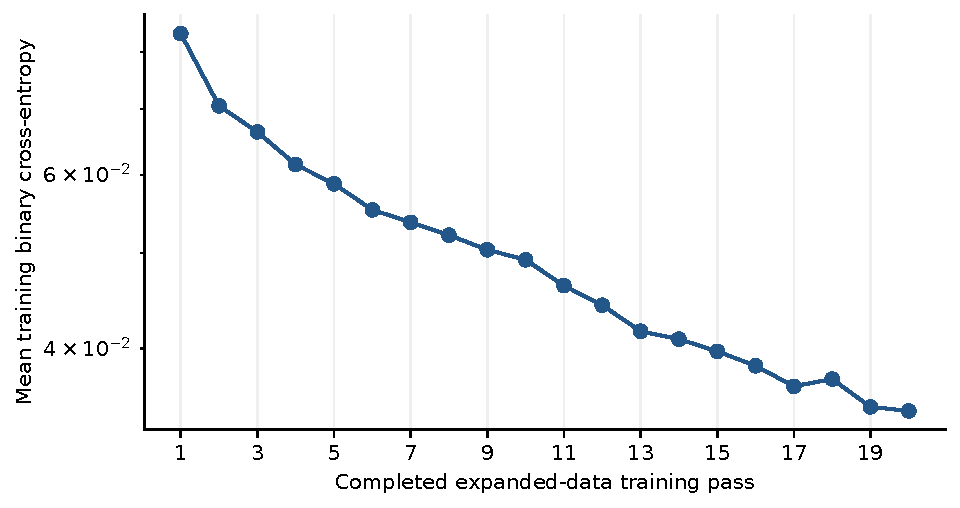
\includegraphics[width=0.80\linewidth]{figures/training_loss.pdf}
 \caption{Mean training binary cross-entropy during each of the ten
 passes. Each training target contributes equal weight to the mean.
 The vertical axis uses a logarithmic scale. The curve records losses
 during parameter updates; it is not a validation curve.}
 \label{fig:training-loss}
\end{figure}

Before training, the preparation checked every target-label
correspondence and verified that every recorded seed appears in its
candidate pool. Implementation checks verified the binary labels, both
class probabilities, the confidence values and the parameter derivatives.
They also confirmed that the input retains coefficient and term-order
information and that a reordering of candidates only reorders their
scores. During training, the held-out targets supplied no parameter
updates, threshold choices or stopping decisions.

The implementation reads examples in bounded groups and scores
candidate seeds and ordered term pairs in blocks. It retains every
ordered pair in Eq.~\eqref{eq:seed-pair-embedding}, so the pair count
grows as $n_T(n_T-1)$. The current bounds are 512 terms, 10,000 candidates
and 16 indices per integral. Inputs beyond these bounds are rejected.
The trained model now permits a direct comparison of its predicted
seed sets with the recorded sets in the separate test collection.
\FloatBarrier

\section{Testing the Seed-Selection Model}
\label{sec:seed-test-results}
To measure seed selection after the expanded training, we froze the
weights at the end of the twenty new passes and evaluated all
114,382 targets from 637 reserved families.
The test contains 24,990 individual integrals and 89,392
integral expressions, with loop orders from one through twelve.
It evaluates mass profiles excluded from parameter updates within
the family domains of Section~\ref{sec:integrals-generation}.
The fixed threshold remains $p_b=1/2$, and no test result changes
the weights or the confidence map~\cite{SeedModelTestData}.

\subsection{Reference agreement and seed ranking}
The test supplies 36,792,115 candidate labels, of which 347,684
belong to the recorded sufficient sets. A true positive is a
selected candidate with reference label one, while a false positive
is a selected candidate absent from that set. A false negative is
a recorded seed that the model omits. With these counts,
\begin{equation}
 {\rm precision}=\frac{\mathrm{TP}}{\mathrm{TP}+\mathrm{FP}},
 \qquad
 {\rm recall}=\frac{\mathrm{TP}}{\mathrm{TP}+\mathrm{FN}},
 \qquad
 F_1=\frac{2\,{\rm precision}\,{\rm recall}}
             {{\rm precision}+{\rm recall}} .
 \label{eq:seed-test-pr}
\end{equation}
The pooled precision is 90.416\%, recall is 76.305\%
and $F_1$ is 82.763\%. The fraction of targets whose complete predicted
set equals its recorded set is 56.831\%. Candidate-label accuracy
is 99.700\%; the all-zero rule gives 99.055\%
because zero labels are frequent. Precision, recall and complete-set
agreement therefore describe seed recovery more directly than
accuracy alone~\cite{SaitoRehmsmeier2015}.

\begin{figure}[htbp]
 \centering
 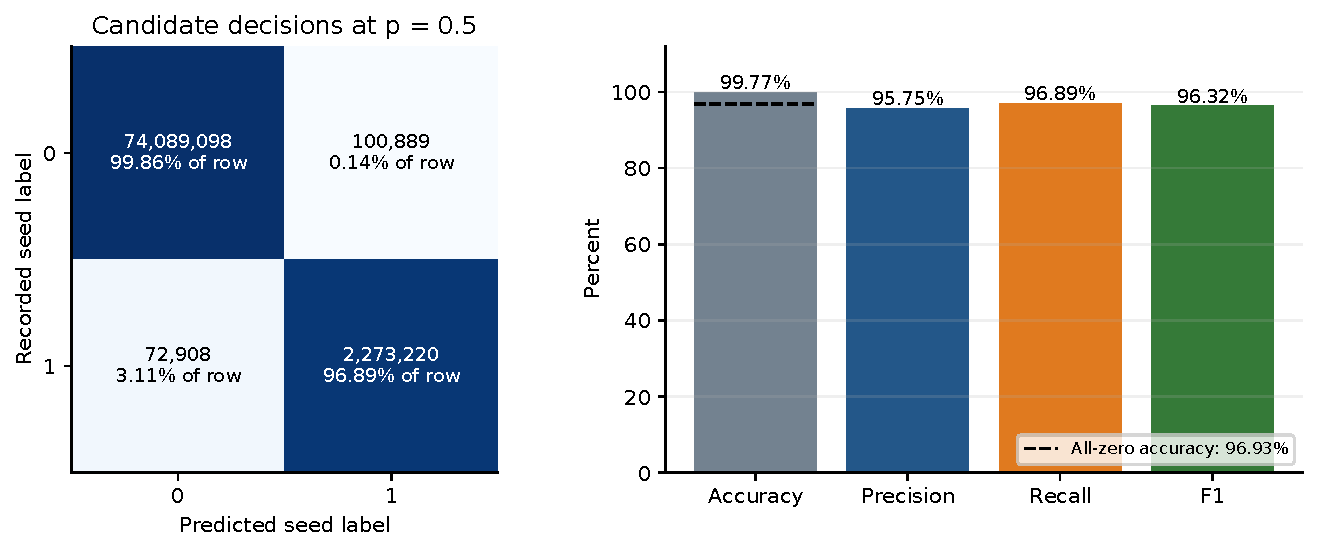
\includegraphics[width=\linewidth]{figures/seed_classification.pdf}
 \caption{Candidate decisions at the fixed threshold, with pooled
 precision, recall and $F_1$. Each confusion-matrix percentage is
 normalized within its reference-label row.}
 \label{fig:seed-classification}
\end{figure}

To examine the scores without changing the threshold, we rank
candidates by $p_b$ and group candidates with equal scores.
For a target $T$, let $P_g$ and $R_g$ be the precision and recall
after including score group $g$ in descending order. With $R_0=0$,
the target average precision is~\cite{AveragePrecisionDefinition}
\begin{equation}
 {\rm AP}_T=\sum_g (R_g-R_{g-1})P_g .
 \label{eq:seed-average-precision}
\end{equation}
Each increase in recovered reference seeds therefore weights the
precision at that point. Averaging over targets with at least one
recorded seed gives mean target average precision 93.737\%.
The first ten candidates recover, on average, 98.009\% of
recorded seeds and contain every recorded seed for 93.337\%
of targets in the corresponding nonempty-reference comparison.
The score-curve calculation uses 4,096 fixed probability intervals;
it supplies a descriptive curve and does not select a new
operating threshold.

\begin{figure}[htbp]
 \centering
 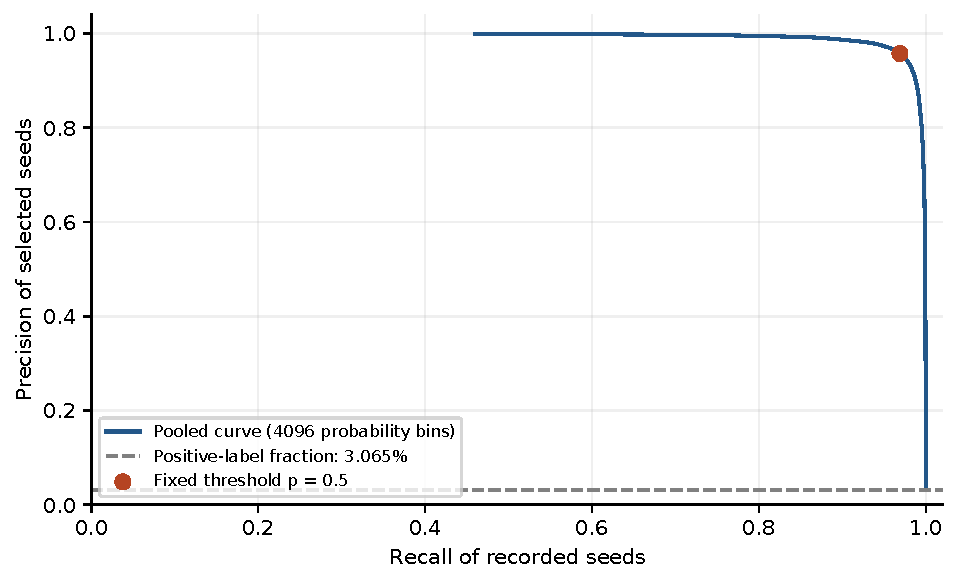
\includegraphics[width=0.80\linewidth]{figures/precision_recall.pdf}
 \caption{Pooled precision and recall as the score threshold varies.
 The marked point retains the fixed threshold of one half.
 The horizontal reference gives the positive-label fraction.}
 \label{fig:seed-precision-recall}
\end{figure}
\begin{figure}[htbp]
 \centering
 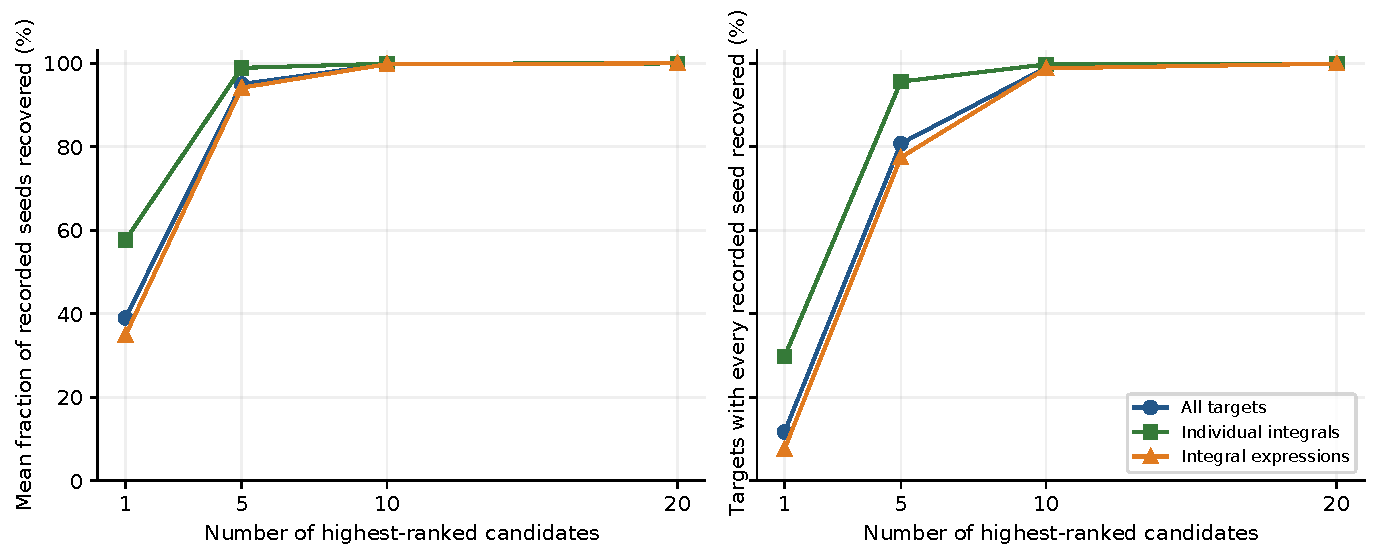
\includegraphics[width=\linewidth]{figures/ranked_seed_recovery.pdf}
 \caption{Recorded-seed recovery as the number of supplied
 highest-ranked candidates increases. The right panel requires every
 recorded seed to appear in the selected prefix. Individual
 integrals and integral expressions are also shown separately.}
 \label{fig:seed-ranking}
\end{figure}

\subsection{Confidence and dependence on the family}
For a returned binary label, the model reports $q_b$ from
Eq.~\eqref{eq:seed-binary-confidence}. We group decisions by this
value and compare their mean confidence with the fraction matching
the reference. Equality would place a group on the diagonal of
Figure~\ref{fig:seed-confidence}. These empirical comparisons assess
the saved scores without fitting a calibration correction.

\begin{figure}[htbp]
 \centering
 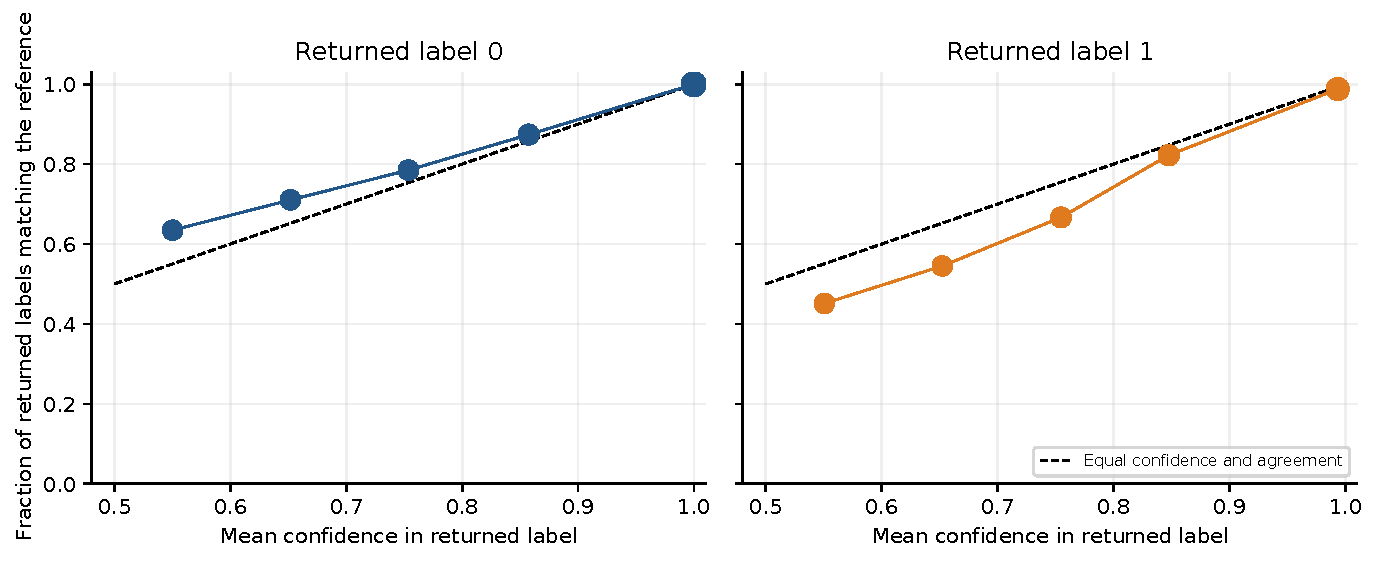
\includegraphics[width=\linewidth]{figures/confidence_calibration.pdf}
 \caption{Reported confidence and observed label agreement, shown
 separately for returned labels zero and one. Marker area increases
 with the number of decisions in a group.}
 \label{fig:seed-confidence}
\end{figure}

Figure~\ref{fig:seed-families} separates performance by family and
loop order. The one-loop group has 306 families,
the two-loop group has 31, and each remaining order
has thirty held-out mass profiles. This separation matters because
the added vacuum families use different identities and candidate
bounds from the earlier one-loop collection. Loop-order comparisons
also reflect these differences in the mathematical domain.
At one loop the pooled recall is 91.802\% and $F_1$ is
93.106\%; at twelve loops they are 60.358\% and
69.568\%, respectively. Across the groups from two through
twelve loops, the lowest recall is 39.026\% at
$L=7$. These missed reference seeds show why a
proposed set still needs an exact sufficiency check before use in
a complete reduction.

\begin{figure}[htbp]
 \centering
 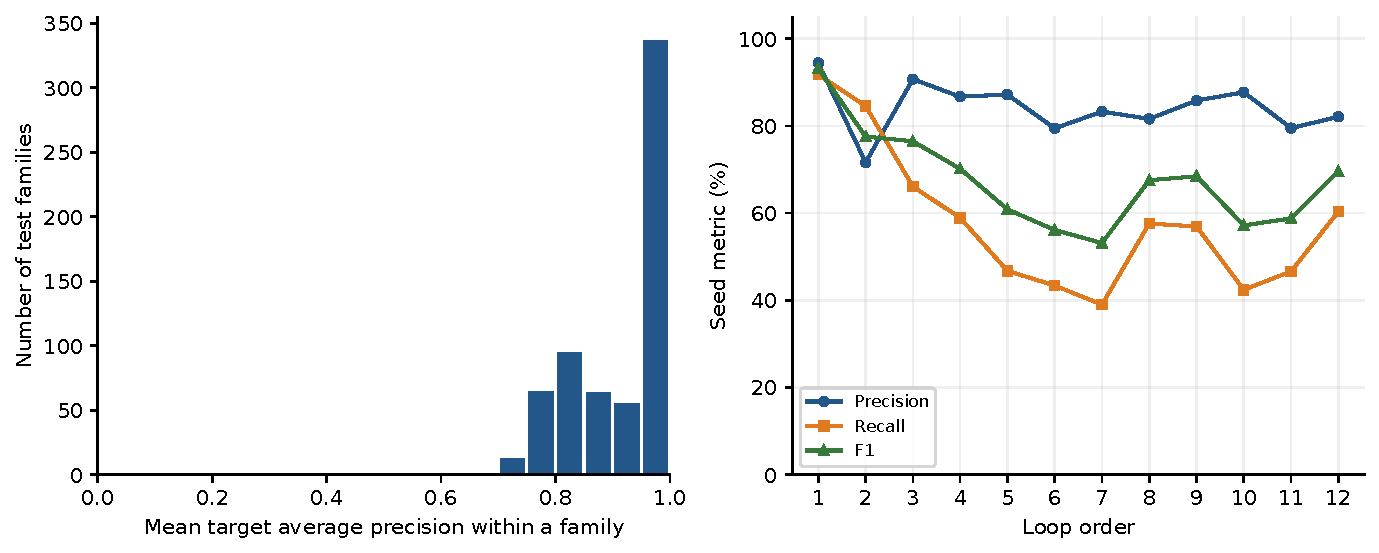
\includegraphics[width=\linewidth]{figures/family_performance.pdf}
 \caption{Distribution of mean target average precision across
 held-out families, and pooled seed precision, recall and $F_1$ at
 each loop order. The higher-loop groups cover the restricted
 vacuum mass profiles defined in the text.}
 \label{fig:seed-families}
\end{figure}

\subsection{Checks and interpretation}
Independent checks reproduce the saved confusion counts and target
counts, verify the prediction hashes and confirm that the weights
remain fixed. All stored probabilities are finite and lie between
zero and one. The mean time for input preparation and model
inference is 3.2807 ms per target on the test allocation;
this excludes a subsequent exact reduction.

The labels identify one recorded sufficient set. Other seed sets can
also reduce the target, so disagreement with these labels does not
by itself establish failure of the proposed reduction. This test
measures reference-set recovery and confidence. It does not run
Kira with the predicted seed sets, prove seed minimality or measure
a solver speedup. The next model addresses the separate choice of
an allowed elimination step after equations are available.
\FloatBarrier

\section{Machine Learning Model for Reduction Propagation}
\label{sec:reduction-model}
The seed model selects identities from which a reduction can proceed.
Once these equations are available, the reduction model selects the next
row operation from a supplied list of allowed steps. We use the current
coefficient matrix and its integral labels to describe each choice, and
the model returns a probability for every listed step. The step with the
largest probability gives the proposed next operation. Exact arithmetic
then updates the matrix, which supplies the input for the next choice.
This section describes the model and its training on the reductions
constructed in Section~\ref{sec:integrals-generation}.

\subsection{Current equations and allowed reduction steps}
Let $A^{(n)}$ be the coefficient matrix after $n$ reduction steps. A column
$j$ corresponds to an integral $I_{\boldsymbol a^{(j)}}$, and a row contains
its coefficients in an identity or in the target expression currently
being reduced. The chosen master basis specifies the columns protected
from elimination. An action $a=(q,r,k)$ uses source row $q$ to eliminate
column $k$ from destination row $r$:
\begin{equation}
 A^{(n+1)}_{rj}
 =A^{(n)}_{rj}
  -\frac{A^{(n)}_{rk}}{A^{(n)}_{qk}}A^{(n)}_{qj},
 \qquad q\ne r,\quad A^{(n)}_{qk}\ne0,\quad A^{(n)}_{rk}\ne0.
 \label{eq:reduction-action}
\end{equation}
All other rows remain unchanged during this elementary step. If both
rows are identities, this is an elementary row operation. If row $r$
represents a target, row $q$ must be a zero identity so that the target
retains its value. The solver supplies the allowed action set
$\mathcal A_n$, enforcing its integral ordering, master basis and row
roles. The model ranks this finite list; completeness of the list remains
the responsibility of the solver.

The stored examples describe a particular instance of this matrix.
They contain one changing target row and the source identities available
for eliminating its largest remaining nonmaster integral under
Eq.~\eqref{eq:target-reference-order}. Each candidate specifies one of
these identities, the target row and that integral. After a choice, the
source identities remain fixed and the target row changes. The prediction
interface also accepts several changing rows, while the present training
data cover the stored target-row procedure. Section~\ref{sec:live-matrix} tests the frozen policy on Kira's evolving
selected IBP matrix using admissible actions that retain its integral
ordering~\cite{Kira3}. This test changes the inference states while retaining
the target-row training described here.

\subsection{Information supplied to the model}
For each allowed action, we construct a vector $\boldsymbol f_a$ from
the current matrix, the pivot integral and the family definition.
The pivot description includes its indices, sector membership, and
the values of $r,s,t,n_{\rm dot}$ in Eq.~\eqref{eq:complexities}.
Descriptions of the source and destination rows give their nonzero
counts, master content and the mean and largest integral complexities.
A matrix summary gives its number of rows, columns and nonzero entries.
The public family definition supplies the numbers of loops and
kinematic parameters together with the propagators and scalar-product
relations. We encode their written form through the same fixed signed
token counts described in Section~\ref{sec:seed-model-architecture},
using 32 components here. This encoding admits collisions between
different groups of symbols. We transform nonnegative counts with
$\log(1+v)$, where $v$ is the count, and each signed index $a_i$ with
$\operatorname{sgn}(a_i)\log(1+|a_i|)$. The representation allows up to
16 indices and records which positions belong to the family.
These definitions give 132 features for each candidate.

The current records supply coefficients in $\mathbb F_P$, the field
of integers modulo a prime $P$. We use these coefficients to calculate
the overlap of each source row with its destination, the number of
terms that the proposed operation would cancel or introduce, and its
immediate arithmetic count. For a source with $n_q$ nonzero entries,
this count is $1+2n_q$: one division and $n_q$ multiplications and
subtractions, using the convention in
Section~\ref{sec:integrals-generation}. These quantities require one
sparse trial row update per action. They use only the current matrix
and do not inspect later reduction steps or reference master
coefficients.
A symbolic coefficient can vanish at the chosen sample, so the model
uses counts recomputed from the sampled rows. The data audit retains
the distinction from the original symbolic support counts. Structural
counts and integral descriptions carry this information into the model.
The numerical size of a modular residue does not represent the
magnitude of a real coefficient.

The representation compresses the supplied matrix into these features,
so different states can have the same description. It includes local
cancellation information and a summary of the candidate set. These
quantities describe the current choices without enumerating complete
reduction paths. Forming these features and evaluating the model
contribute to the eventual runtime
and must be included when measuring a reduction speedup.

\subsection{Action probabilities and confidence}
A shared map $\phi_\theta$ converts each candidate vector into a
32-component vector,
\begin{equation}
 \boldsymbol h_a=\tanh(W_1\boldsymbol f_a+\boldsymbol b_1),\qquad
 \boldsymbol u=\frac{1}{|\mathcal A_n|}
                    \sum_{a\in\mathcal A_n}\boldsymbol h_a,\qquad
 \boldsymbol v=\max_{a\in\mathcal A_n}\boldsymbol h_a .
 \label{eq:reduction-encoding}
\end{equation}
Here $\theta$ denotes the adjustable parameters, $W_1$ is a learned
matrix, $\boldsymbol b_1$ is a learned offset, and the maximum acts
on each component separately. Sharing the map and combining candidates
through averages and maxima makes the scores independent of their
position in the supplied list~\cite{DeepSets}. The model joins
$\boldsymbol h_a,\boldsymbol u,\boldsymbol v$ and applies a second
map with 64 hidden components to obtain a scalar score $g_\theta(a)$.
For a fixed family, master basis and finite-field sample, it returns
\begin{equation}
 \begin{aligned}
 p_\theta(a\mid A^{(n)},\mathcal A_n)
 &=\frac{\exp g_\theta(a)}
        {\sum_{b\in\mathcal A_n}\exp g_\theta(b)},\\
 \widehat a_n&=\mathop{\rm arg\,max}_{a\in\mathcal A_n}p_\theta(a),
 \qquad q_n=p_\theta(\widehat a_n).
 \end{aligned}
 \label{eq:reduction-choice}
\end{equation}
Thus the probabilities sum to one over the supplied alternatives,
and $q_n$ is the reported confidence for the selected step.
With one allowed step the probability is one by construction, which
provides no evidence of learned discrimination. An empty candidate
list returns no proposed operation; the solver must determine whether
the reduction is complete or further identities are required.

Training gives these probabilities an interpretation as agreement
with the recorded next choice, conditional on the supplied state and
actions. Several choices can give valid reductions, and an alternative
choice may even lead to a shorter sequence. The reference paths establish
valid reductions and their recorded costs; they do not establish global
minima. Section~\ref{sec:reduction-test} compares this confidence with agreement
on reserved choices. Confidence does not certify exactness, minimal
cost or the success of a complete reduction. Equation~\eqref{eq:reduction-action}
and the solver's checks retain responsibility for the algebra.

\subsection{Training examples and separation from testing}
We retain the same grouped family division used for the seed model:
11,963 families with 1,610,890 targets supply training records, while
5,137 families with 690,382 targets remain reserved for testing.
Every state from one target stays with that target's family.
We read the row before each recorded step and its complete stored list
of admissible source equations. The chosen equation supplies the
reference action $a_n^\star$. The row after the step and the stored
operation counts check the data preparation but remain outside
the predictive inputs. The target's construction history, final master
coefficients and future choices also remain outside those inputs.

For the set $\mathcal D_{\rm choice}$ of training states with at least
two allowed actions, the objective is
\begin{equation}
 \mathcal L_{\rm red}(\theta)
 =-\frac{1}{|\mathcal D_{\rm choice}|}
   \sum_{(A,\mathcal A,a^\star)\in\mathcal D_{\rm choice}}
           \log p_\theta(a^\star\mid A,\mathcal A).
 \label{eq:reduction-loss}
\end{equation}
Each such state has equal weight. States with one admissible action
have zero loss and remain in the data audit. The recorded reference
choice is the training label; absence of a label on another action does
not establish that its reduction is invalid.

We use AdamW~\cite{AdamW} with a learning rate of $10^{-3}$, weight decay
$10^{-4}$, batches of 256 states and a gradient norm limit of one.
We continued the saved expanded-data model and optimizer for twenty
complete passes over the enlarged training states. The new phase
retains the architecture and optimizer settings while adding 1,250
mass profiles at every represented loop order. Preparation replays every selected row
operation with exact modular arithmetic and verifies its final
recorded master row. Training shuffles states within bounded
groups of families and retains complete resume states.
The reserved families remain outside parameter updates and
confidence fitting. Earlier project stages evaluated the preceding
held-out families; the current experiment also reserves the newly
assigned mass profiles at every added loop order.

\subsection{Completed training and present scope}
The expanded training set contains 14,684,059 recorded states from
1,610,890 targets in 11,963 families. Of these states,
5,840,122 supply at least two allowed actions and
8,843,937 supply one action. The records contain
26,775,999 candidate appearances. The unchanged model
uses 132 features per candidate and has 10,529 adjustable parameters.

Preparation replays every reference row operation, checks continuity
between steps and verifies the final master support. Symbolic
coefficients can vanish at the sampled kinematic point, so the model
uses the support of the actual sampled matrix. The audit records
these differences without changing the exact symbolic references.

We continued the preceding expanded-data model and its AdamW
optimizer for twenty complete passes over the enlarged data. Each new pass
uses every training state with an action choice; a forced step has
probability one and supplies no ranking decision. The new phase
contains 116,802,440 choice-state presentations and
463,763 parameter updates. The preserved lineage contains thirty
passes over the original smaller collection and twenty passes over
the preceding 2,100-family collection. The latest twenty passes
use the enlarged collection across all represented loop orders.

Mean training cross-entropy changed from 0.3823373 to
0.3804633 during this phase, while agreement with the recorded
action changed from 99.841\% to 99.895\%.
These values describe losses and choices encountered during
parameter updates. Section~\ref{sec:reduction-test} measures the
frozen parameters on reserved families.

The implementation retains the original architecture, learning rate,
gradient bound and state-batch limits. Training uses four CPU threads,
while inference uses one. Parallel preparation reproduces the saved
training features and labels exactly. Checks verify equal weights
in the inference and resumable checkpoints, complete state coverage
and the preserved optimizer lineage. The published implementation
retains the inputs, learned parameters and exact reference
records~\cite{ReductionModelData}.

The training domain still consists of one changing target row and a
fixed source-equation pool. The new records extend this domain
through twelve loops for the coupled vacuum families specified
above. They provide evidence about these allowed reduction steps;
general sparse elimination inside Kira requires a separate
integration and benchmark.


\section{Testing the Reduction-Propagation Model}
\label{sec:reduction-test}
To test the model after twenty expanded-data passes, we froze its
parameters and evaluated 690,382 targets in 5,137 held-out
families. Every loop order from one through twelve occurs in this
set. We first compared the predicted next step with the recorded
choice, then allowed the model to choose a complete path from the
initial target row. Both tests retain exact finite-field row
operations~\cite{ReductionModelTestData}.

\subsection{Allowed steps and the comparison rule}
At a given state, the candidates are the source identities whose
leading nonmaster integral matches the target row's leading
nonmaster integral. Both the learned policy and the comparison rule
receive this same list and respect the recorded integral order.
The source rows remain fixed while elimination changes the target
row. This restriction makes the available actions and complete
reference answers explicit.

For each allowed source row $E$, let $u_E$ be the target row after
the corresponding exact elimination. The local comparison rule
selects the smallest tuple
\begin{equation}
 \left(n_{\rm nm}(u_E),\
       \operatorname{nnz}(u_E),\
       1+2\operatorname{nnz}(E),\
       \operatorname{id}(E)\right).
 \label{eq:reduction-local-rule}
\end{equation}
Here $n_{\rm nm}$ is the number of nonmaster columns with nonzero
coefficients, $\operatorname{nnz}$ is the total number of nonzero
coefficients and $\operatorname{id}(E)$ is a fixed equation
identifier used only to resolve ties. The third entry counts one
division and one multiplication and subtraction for each source
entry. The rule compares the immediate next rows; it does not search
all complete reduction paths.

\subsection{Next-step agreement and confidence}
The reserved traces contain 6,364,695 states, including
2,558,472 with an action choice and 3,806,223 with one allowed
action. On states with a choice, the learned model selects the
recorded action in 95.845\% of cases and places it among its first
three candidates in 99.980\%. Its selected action gives the same
next sampled row as the reference in 95.846\% of cases.
The local rule selects the recorded action in 99.473\%
of these states.

When $n_{\rm tie}$ actions share the largest saved probability,
the program selects one through its fixed identifier order.
Such ties occur in 37.747\% of choice states.
We also assign credit $1/n_{\rm tie}$ when the recorded action
belongs to the highest-scoring set, and zero otherwise. Averaging
this credit gives 74.506\% reference agreement.
This diagnostic describes the scores while retaining the stated
deterministic choice rule for the actual reductions.

\begin{figure}[htbp]
 \centering
 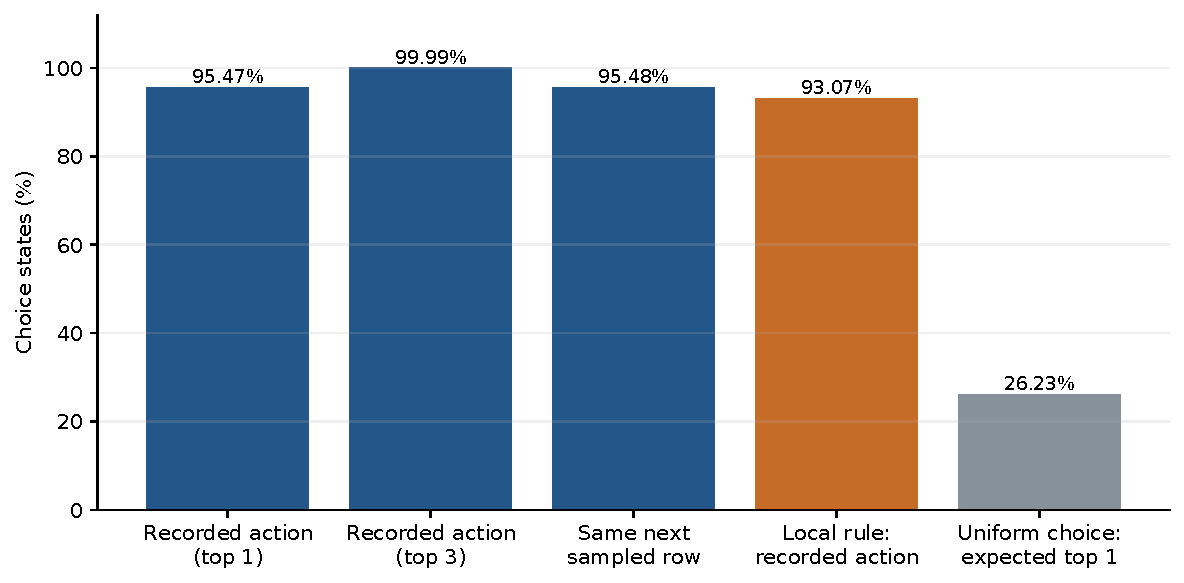
\includegraphics[width=\linewidth]{figures/reduction_action_accuracy.pdf}
 \caption{Next-step comparisons on states with at least two allowed
 actions. The uniform reference assigns equal probability to every
 available action. The tie-averaged result shares credit equally
 among highest-scoring tied actions. The same-row comparison permits different
 identities that produce the same sampled next row.}
 \label{fig:reduction-action-accuracy}
\end{figure}

The model assigns a probability to every supplied action, with
probabilities summing to one. We compare the selected action's
reported probability with observed agreement after grouping
predictions into ten fixed confidence intervals. Let
$\mathcal D^{\rm test}_{\rm choice}$ be the set of held-out states
with at least two allowed actions, and let $a_n^\star$ be the
recorded action at state $n$. Applying the negative logarithmic
loss in Eq.~\eqref{eq:reduction-loss} to this set gives 0.400146.
The calculation replaces probabilities below $10^{-38}$ by
$10^{-38}$ when taking their logarithms.

To compare the full probability distribution with the recorded
choice, we also calculate the multiclass Brier score~\cite{Brier1950},
\begin{equation}
 B_{\rm test}
 =\frac{1}{|\mathcal D^{\rm test}_{\rm choice}|}
 \sum_{n\in\mathcal D^{\rm test}_{\rm choice}}
 \sum_{a\in\mathcal A_n}
 \left[p_\theta(a\mid A^{(n)},\mathcal A_n)
       -\mathbf 1_{a=a_n^\star}\right]^2 .
 \label{eq:reduction-brier}
\end{equation}
Here $\mathcal A_n$ is the supplied action set and
$\mathbf 1_{a=a_n^\star}$ equals one for the recorded action and
zero for every other action. We sum over all actions without
dividing by their number, then give each state equal weight.
The resulting score is 0.250632. The confidence comparison in
Figure~\ref{fig:reduction-confidence} uses the frozen scores without
fitting a correction. A forced action has probability one, so these
ranking and confidence comparisons exclude forced states.

\begin{figure}[htbp]
 \centering
 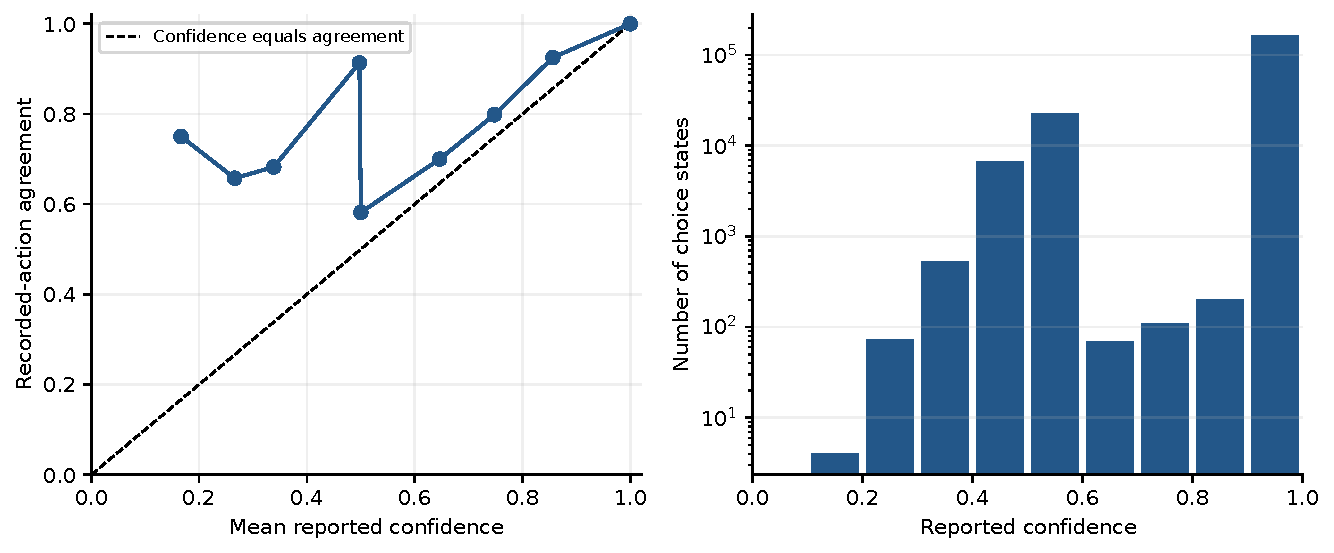
\includegraphics[width=\linewidth]{figures/reduction_confidence.pdf}
 \caption{Reported confidence and recorded-action agreement, with
 the number of choice states in each confidence interval. The
 diagonal represents equality between confidence and agreement.}
 \label{fig:reduction-confidence}
\end{figure}

\begin{figure}[htbp]
 \centering
 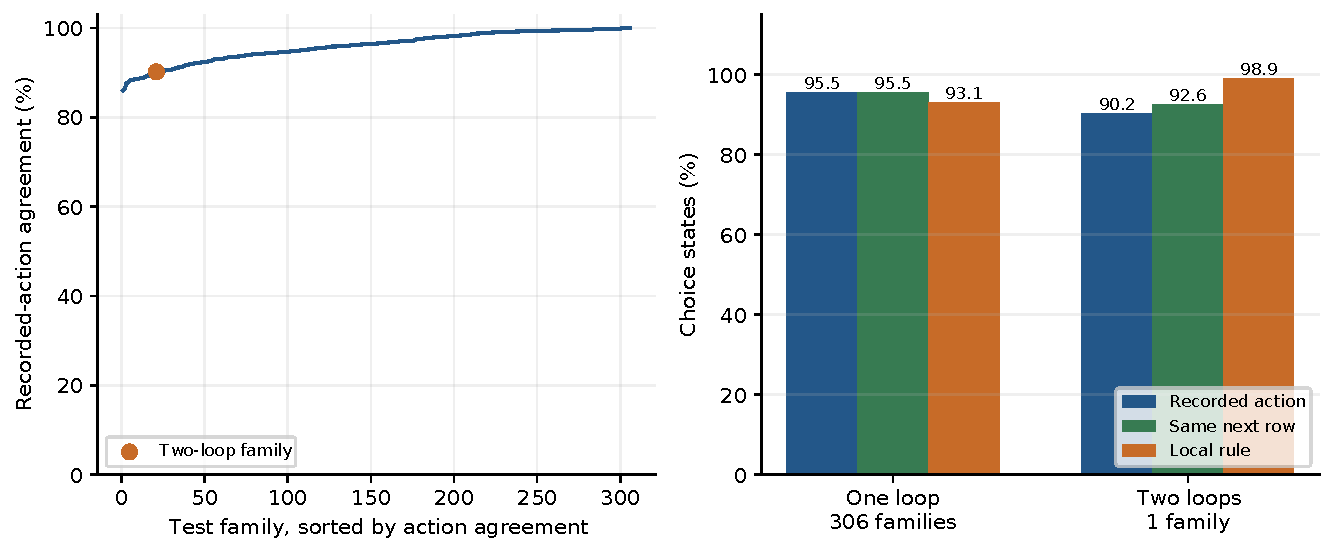
\includegraphics[width=\linewidth]{figures/reduction_families.pdf}
 \caption{Agreement across individual families and loop orders.
 Every higher-loop group uses held-out mass profiles of the
 restricted vacuum families. These comparisons include changes in
 the mathematical family domain as well as loop order.}
 \label{fig:reduction-families}
\end{figure}

\subsection{Complete reductions and arithmetic work}
For complete-path testing, the policy receives the initial target row
and repeatedly selects an allowed identity until the row contains
only protected masters or a stated failure condition occurs.
Decisions use the first finite-field sample. We then replay the
selected sequence at both additional samples and compare the
resulting rows with the exact reference master coefficients
evaluated at those points.

The learned policy matches all three sampled master expansions for
690,302 of 690,382 targets (99.988\%).
The local rule matches all three for 689,700 targets
(99.901\%). The respective numbers without this full
three-sample agreement are 80 and
682. For the learned policy, 77
targets stop when the supplied pool has no allowed identity for the
remaining leading integral, and 3 complete at
the decision sample but fail an additional-sample check. The local
rule gives 664 and 18 in these
two categories. Agreement at the samples is the stated test
criterion; the test does not reconstruct a new symbolic rational
result from the learned path.

\begin{figure}[htbp]
 \centering
 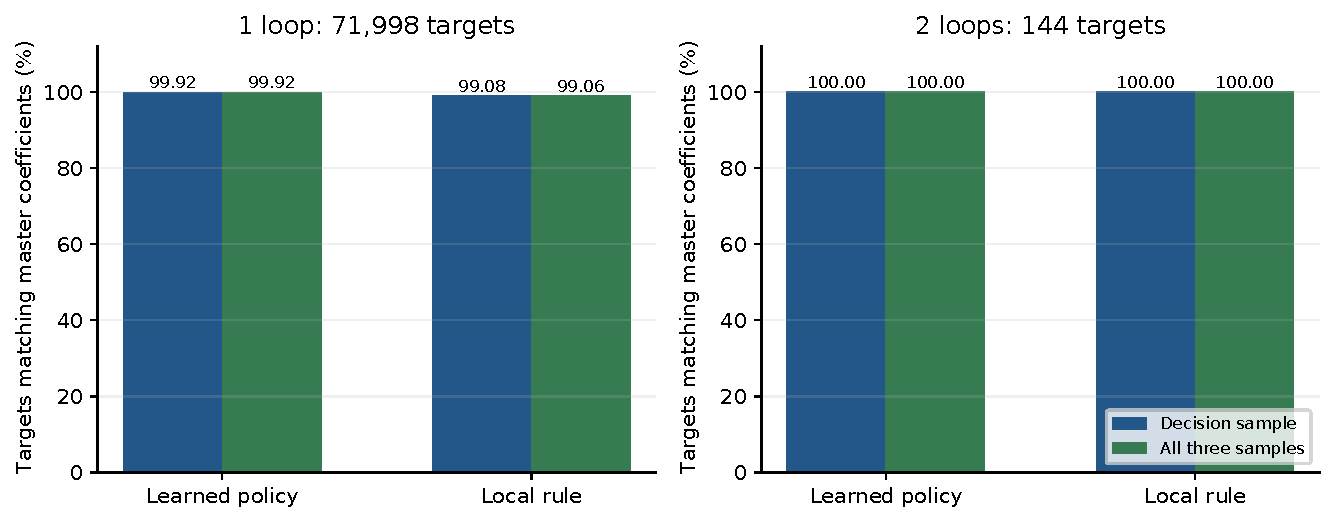
\includegraphics[width=\linewidth]{figures/reduction_rollout_success.pdf}
 \caption{Complete target reductions at each loop order. The left
 panel requires agreement at the decision sample; the right panel
 requires agreement at all three samples.}
 \label{fig:reduction-rollout-success}
\end{figure}

We compare arithmetic counts on the 689,684 targets for which
both policies pass all three samples and the reference count is
nonzero. The learned policy uses fewer committed row operations
than the local rule for 6,846 targets, the same number for
610,196 and more for 72,642. A committed operation changes the
selected target row. Candidate trials used to construct model
features or evaluate the local rule also perform arithmetic, so
Figure~\ref{fig:reduction-operations} shows both accounting choices.
The recorded path supplies a valid reference count without a proof
that this count is minimal.

\begin{figure}[htbp]
 \centering
 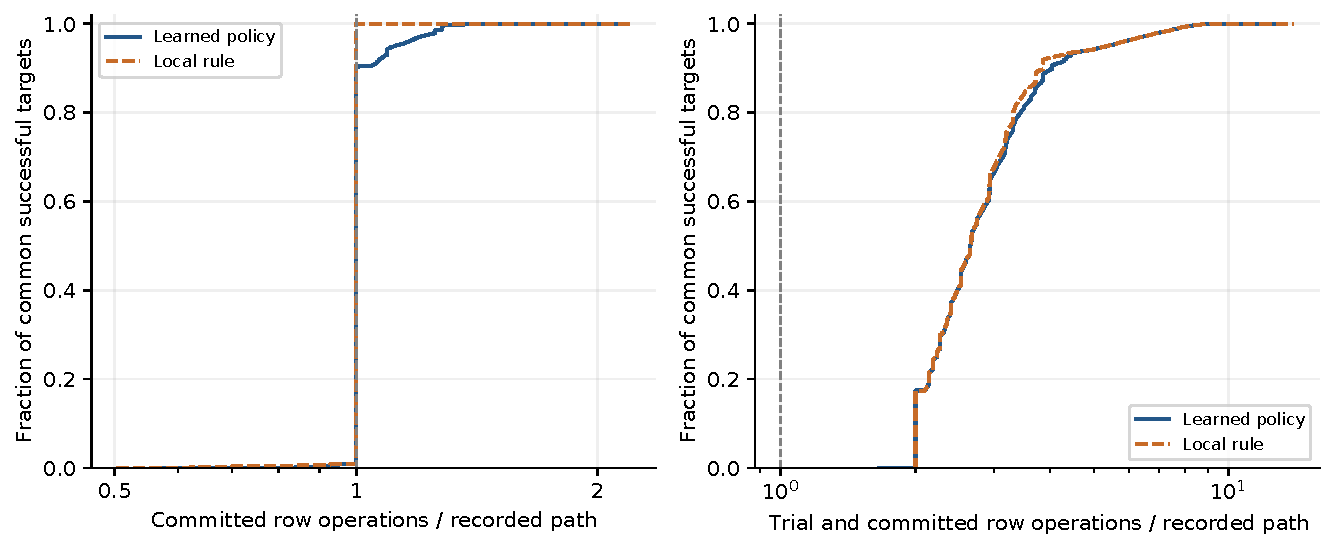
\includegraphics[width=\linewidth]{figures/reduction_operation_counts.pdf}
 \caption{Cumulative distributions of arithmetic counts relative
 to the recorded path, restricted to targets successful for both
 policies. The right panel also includes trial row operations used
 when choosing an action. Both horizontal axes use logarithmic scales.}
 \label{fig:reduction-operations}
\end{figure}

\subsection{Timing, checks and scope}
The mean attempted reduction time is 12.3438 ms per target for
the learned policy and 0.6991 ms for the local rule. The
learned policy therefore takes 17.657 times as long on this
allocation. These times include action selection and committed
elimination within the target-row experiment. We alternate policy
execution order between targets and keep verification and disk
output outside the timed interval. Four CPU workers on the same
compute node process disjoint families, with one computation thread
per worker. Both policies run in the same worker for each target. Figure~\ref{fig:reduction-runtime}
shows the timing distributions on the test allocation.

\begin{figure}[htbp]
 \centering
 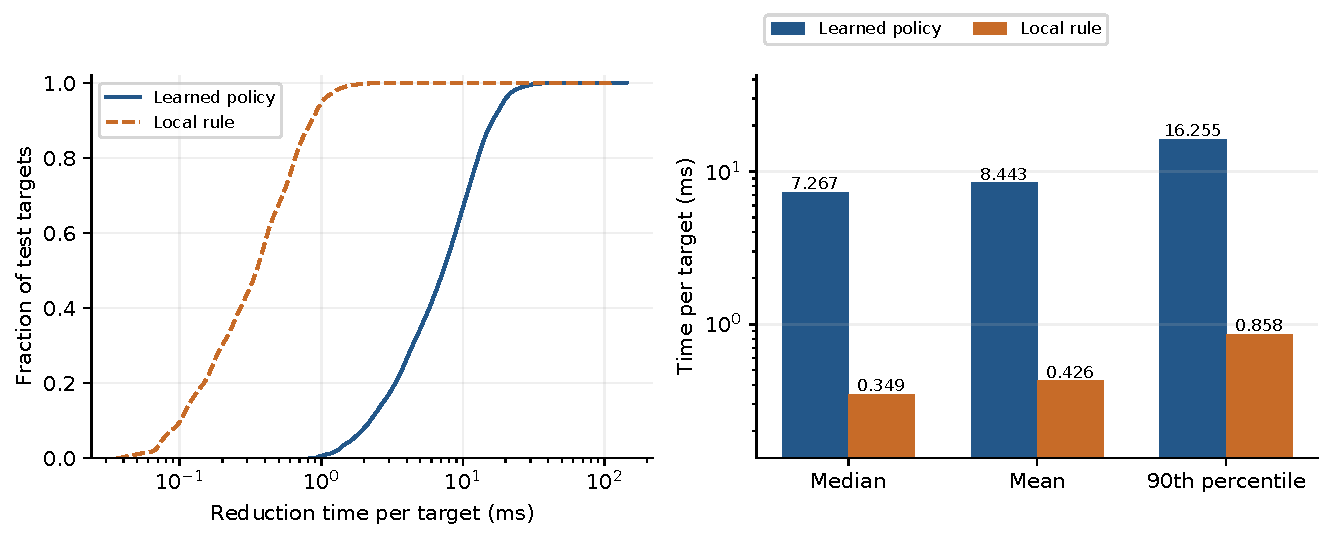
\includegraphics[width=\linewidth]{figures/reduction_runtime.pdf}
 \caption{Attempted target-row reduction times for the learned
 policy and local rule. Both receive identical initial rows,
 source pools and integral ordering.}
 \label{fig:reduction-runtime}
\end{figure}

Independent checks reproduce probability summaries and replay the
committed finite-field operations from the saved paths at the
decision sample. They also
verify the source coefficients, data split and unchanged model hash.
The tests distinguish agreement with a recorded next action from
completion of an allowed alternative path.

The results concern the supplied equation pools and family domains.
Every tested loop order also occurs in training, and related
lower-sector integrals can occur in different mass profiles.
Consequently, the experiment measures held-out profile performance
within these domains. It does not establish globally optimal seed
sets, globally minimal elimination paths or an end-to-end Kira
speedup.
Section~\ref{sec:cost-comparison} then measures complete symbolic reductions with Kira, including model and fallback costs.
\FloatBarrier

\section{Comparison with Kira}
\label{sec:cost-comparison}
A useful learned choice must reduce the cost of obtaining the final
master coefficients. The sufficiency test in
Section~\ref{sec:seed-kira-sufficiency} establishes which stored seed
sets permit a reduction, while the preceding target-row test measures
individual reduction paths. We now compare complete symbolic reductions
with Kira's existing equation selection and seeding. The comparisons
retain both trained models, the held-out families and the seed
threshold of one half. The candidate seed lists and prescribed
master bases are inputs; their earlier construction is outside
the measured reduction costs.

\subsection{Targets, baselines and exact checks}
We use 19 held-out family instances: one restricted vacuum profile
at each loop order from one through twelve, three box profiles,
and one bubble, triangle, tadpole and two-loop propagator family.
The three box profiles represent the smallest, middle and largest
candidate-pool sizes in that domain. A fixed hash order selects the
other profiles and the target expressions without consulting previous
model outcomes. Nested batches contain 1, 4 and 16 targets, with
batches of 1 and 3 for the three-target tadpole family.
This gives 56 batch cases and 291 distinct targets.
The restricted vacuum profiles retain the dependent denominators
described in Section~\ref{sec:higher-loop-generation}; their loop orders
do not represent the complexity of general multiloop scattering.

For the supplied-equation comparison, Kira receives the connected
part of the complete stored source pool and applies its own
equation selection, forward elimination and back substitution.
The learned seed method takes the union of the predicted seed sets
for the requested batch and supplies the corresponding stored
IBP identities together with the same background identities.
If any target retains an integral outside the prescribed master
basis, the method reruns the batch with the complete pool.
Both attempts contribute to its cost. This comparison isolates
selection from a common source library; generating that library
is outside these timings.

For the row comparison, the learned model chooses source identities
using a fixed finite-field sample, while
Eq.~\eqref{eq:reduction-action} updates the target coefficients
symbolically in $\mathbb K=\mathbb Q(\boldsymbol x,d)$.
Kira then reduces any remaining terms. A second version applies the
local rule from Section~\ref{sec:reduction-test} through the same
symbolic procedure. This control identifies the cost of the learned
choice relative to the local choice. Both methods retain fixed
source identities and a changing target row, which is the procedure
covered by the training data.

We compare each final coefficient with its constructed rational
reference and independently evaluate the coefficients and saved
row operations at three finite-field points. The physical master
coefficients remain present throughout this experiment.
A reported completion therefore includes the full symbolic target
expansion and its checks. Each batch-method pair runs three times
on the same compute node, with the execution order rotated.
Kira and the model each use one computation thread. At most two
trials run concurrently on the cluster.

\subsection{Learned seed bounds in native Kira}
The seven families with independent propagator bases also permit
native Kira equation generation. Kira reduces the component integrals,
and its exact algebra combines their results into the requested target
expressions. We record generation and reduction separately from this
final combination. Native equation counts refer to the component
reduction; the later combination has separate counts and contributes
to every reported total time. For the default baseline, the seeding bounds are
one above the largest values of $r$ and $s$ among the target components
and prescribed masters. The restricted baseline also bounds
$n_{\rm dot}$ one above its largest required value and uses Kira's
subsector truncation with $l=N-s_{\max}$, where $N$ is the number
of propagators. A third control sets $r$, $s$ and $n_{\rm dot}$ directly to the
largest target/master values, uses the same subsector truncation,
and falls back to the default bounds if needed. Both this control
and the learned method reserve 60 seconds for the first native attempt
and 100 seconds for its fallback, within the complete 180-second limit.
These fixed settings retain Kira's own symmetry
handling and equation selection~\cite{Kira3}; they do not represent
an exhaustive search over its settings.

To apply the seed model before native equation generation, let
$\widehat{\mathcal S}_S$ be the predicted seeds in sector $S$.
For every nonempty set, we pass the bounds
\begin{equation}
 \begin{aligned}
 r_S&=\max_{\boldsymbol\sigma\in\widehat{\mathcal S}_S}r(\boldsymbol\sigma),
 &s_S&=\max_{\boldsymbol\sigma\in\widehat{\mathcal S}_S}s(\boldsymbol\sigma),\\
 n_{{\rm dot},S}
 &=\max_{\boldsymbol\sigma\in\widehat{\mathcal S}_S}
           n_{\rm dot}(\boldsymbol\sigma).
 \end{aligned}
 \label{eq:native-learned-bounds}
\end{equation}
to Kira. These bounds enclose the selected seeds, and Kira can generate
additional seeds within the bounds and inherited subsectors.
Its own generated and selected equation counts therefore measure
the resulting work. An incomplete first attempt triggers the default
native bounds. This direct comparison repeats all four native
methods on the largest fixed target batch in each of the seven
families, giving 99 distinct targets and 84 trials. The learned
method uses the same model and threshold as the supplied-pool test.

\subsection{Measured cost and results}
We record the complete elapsed time from process start to a checked
result. It includes input loading, model loading, feature preparation,
inference, exact algebra, any fallback, coefficient checks and output.
We also record the time with the family already loaded and the model
ready for use. This second quantity represents repeated use of prepared
inputs; the complete process time retains the cost of starting the model.
For a matched case, we compare the median of the three repeats and
define
\begin{equation}
 \rho_T=\frac{\operatorname{median}T_{\rm learned}}
              {\operatorname{median}T_{\rm baseline}}.
 \label{eq:cost-ratio}
\end{equation}
Thus $\rho_T<1$ indicates a lower measured time for that case.
Aggregate ratios use the geometric mean of the paired case ratios.
Trials that reach their time or memory limit remain in the completion
counts and are excluded from ratios that require two completed results.

We distinguish supplied equations, equations selected by Kira,
logged forward insertions and coefficient-field operations.
For a committed target-row step with $n_q$ nonzero source entries,
the last count is $1+2n_q$, as in
Section~\ref{sec:reduction-model}. Feature construction also performs
trial updates of candidate rows. These counts do not measure the
internal polynomial work needed to simplify a rational coefficient.
Runtime includes that work. Memory is the largest sampled sum of
resident process memory for the driver, Kira and its algebra process;
the sampling interval is 50 ms, and shared pages can contribute to
more than one process's count. Every trial has a 180-second limit,
a 1.5 GiB address-space limit per process and a 32 MiB scratch limit.
The comparisons use the existing symbolic Kira~3.1 build with Fermat.
They do not benchmark finite-field reconstruction.

The main comparison contains 792 trials. The full stored-pool
baseline completed 168/168, learned seeds completed 168/168,
learned rows completed 168/168, and local-rule rows completed
168/168. On the 56 completed matched batch cases,
learned seed selection gave complete-process and prepared-input time
ratios of 1.720 and 1.116, respectively. It used the full-pool fallback
in 24 trials.
Across those batches, its supplied source-equation count, including
fallback, was 0.251 times the baseline count, while the
number of equations selected by Kira was 1.027 times
the baseline. The distinction shows how Kira's existing selection
changes the work left after an external seed choice.
The learned method had lower complete-process median time in
0 of 56 batches and lower prepared-input
median time in 15 of 56 batches.

The learned row procedure gave time ratios of 1.719 and 1.205
against the full stored-pool baseline over 56 matched
cases. Its ratios against the local row rule were 1.520 and 1.043.
Before the final Kira call, the learned row procedure completed every
target in 54 of the 56 batches, while the local rule did
so in 55. Kira completed the remaining terms in the
other batches.
For the 53 batch cases in which both row procedures themselves
finished all targets before the final Kira call, their summed
committed coefficient-operation counts were 19,401 and
18,881, giving a ratio of 1.028.
This comparison excludes paths that left part of the reduction to
Kira. The elapsed-time measurements retain all of that later work,
as well as candidate feature preparation and exact coefficient
simplification~\cite{KiraCostComparisonData}.

Kira's own equation selection removes much of the redundant input
in the full-pool baseline. The learned seed filter reduces the
supplied pool, and its measured complete cost includes the added
model work and every fallback. Both learned methods have aggregate
complete-process and prepared-input ratios above one in this
comparison. The row-operation ratio also exceeds one relative to the
local rule on the matched complete preprocessing paths. These results
identify added cost in the current implementations and give no
aggregate reduction in the stated time or committed-operation measures.


\begin{figure}[!htbp]
\centering
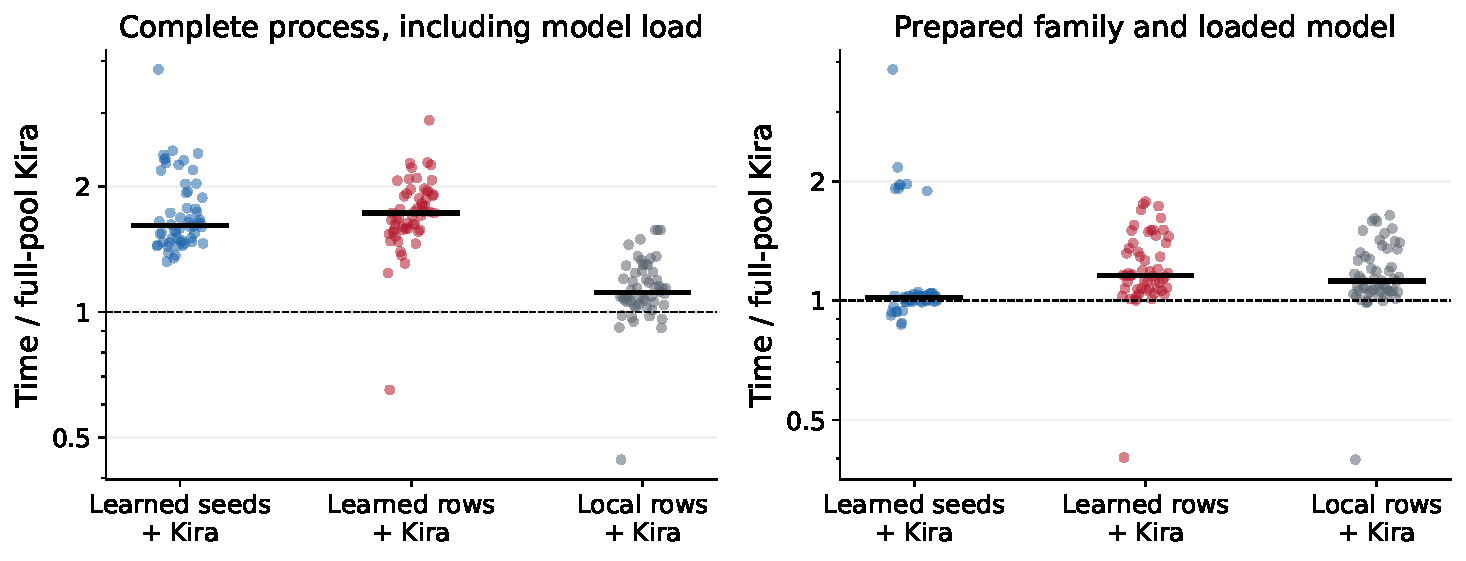
\includegraphics[width=\linewidth]{figures/kira_comparison_time.pdf}
\caption{Matched time ratios relative to Kira with the full stored source pool. Each point uses a batch's three-repeat median. The left panel includes process and model loading; the right panel uses prepared family inputs and a loaded model. Short solid lines show the median case ratio; the dashed line denotes equal time.}
\label{fig:kira-cost-time}
\end{figure}

\begin{figure}[!htbp]
\centering
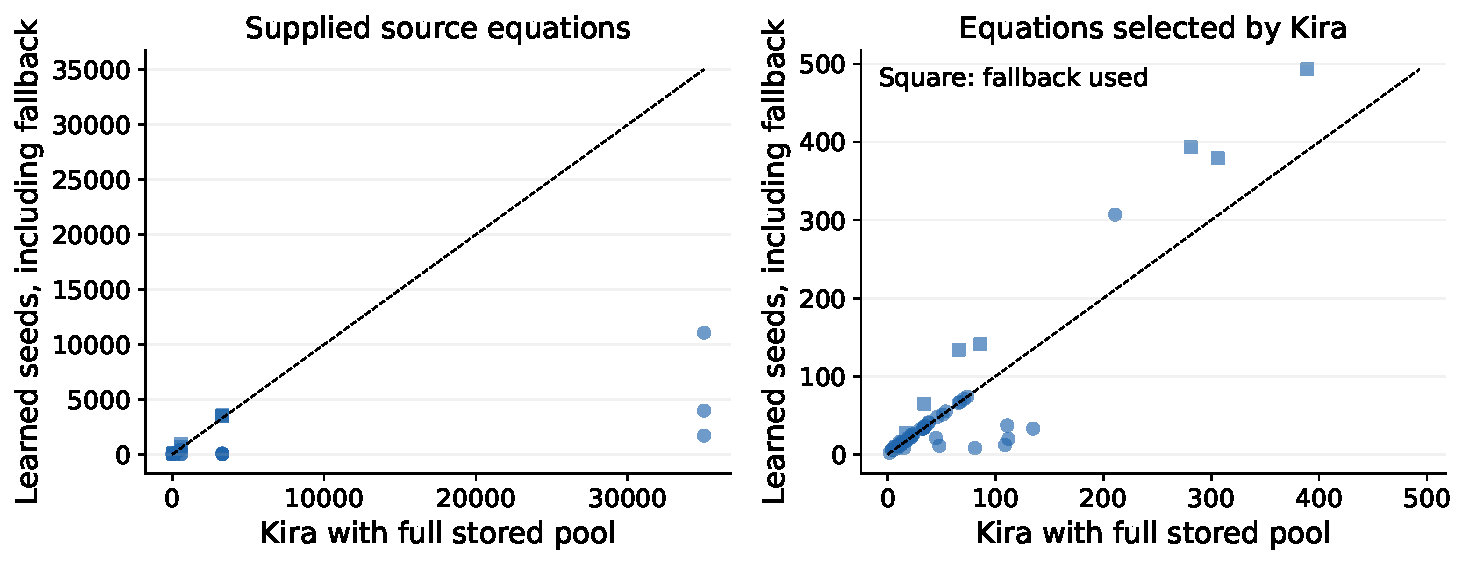
\includegraphics[width=\linewidth]{figures/kira_comparison_equations.pdf}
\caption{Supplied source equations and equations selected by Kira for identical batches. Learned-seed counts include any full-pool fallback. Squares identify batches with fallback, and the diagonal denotes equal counts.}
\label{fig:kira-cost-equations}
\end{figure}

\begin{figure}[!htbp]
\centering
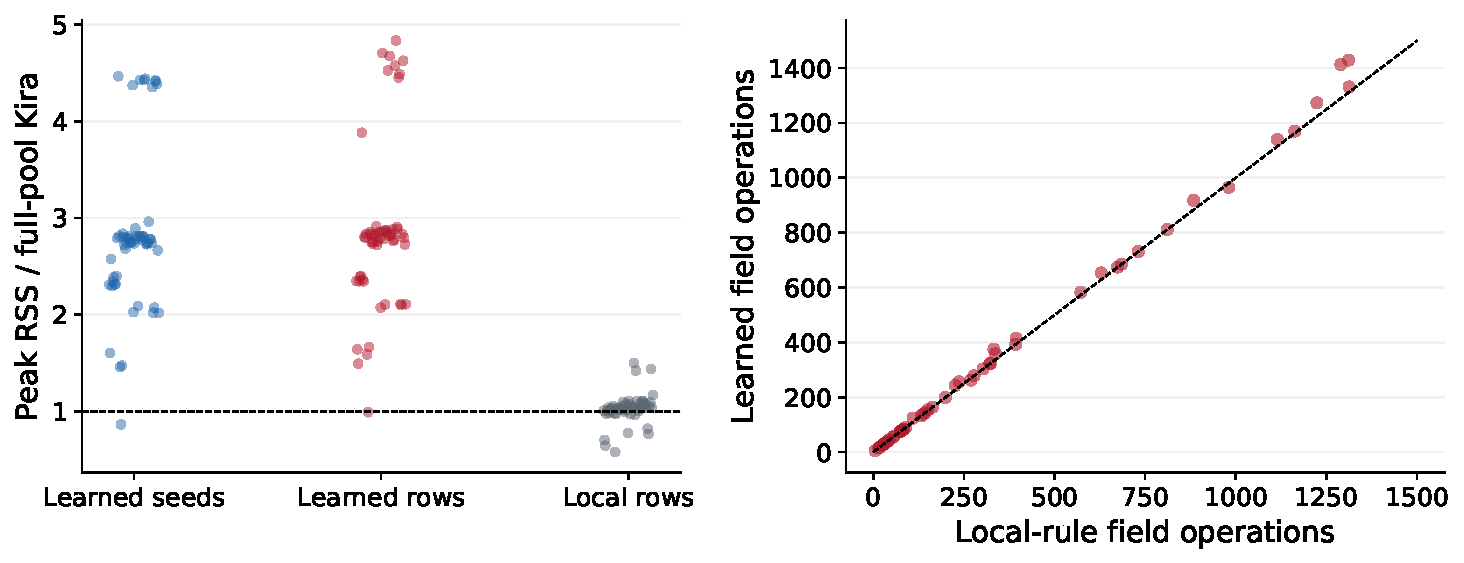
\includegraphics[width=\linewidth]{figures/kira_comparison_memory_operations.pdf}
\caption{Sampled summed resident-memory ratios and committed coefficient-operation counts. Memory ratios use the largest recorded peak within each three-repeat group. The operation panel compares only batches that both row procedures completely reduced before the final Kira call. These counts exclude polynomial simplification and candidate-scoring work.}
\label{fig:kira-cost-memory}
\end{figure}

\FloatBarrier
\subsection{Native seeding results}

The direct native-seeding comparison completed 21/21 learned
trials, 21/21 default-baseline trials, 21/21 restricted-baseline
trials and 21/21 target-index-bound control trials. Learned bounds required a default-bound fallback in
9 trials.
For the 7 paired completed family batches, its
complete-process and prepared-input time ratios against default
native Kira were 1.596 and 1.344. Against restricted native Kira,
the corresponding ratios were 1.671 and 1.373 over 7
paired batches. Against the control that sets bounds directly from target
indices, the ratios were 1.425 and 1.141 over 7 paired batches.
These measurements include native equation
generation, exact reduction, target combination, coefficient checks
and any repeated attempt.

The learned native method had lower complete-process median time
in 0 of 7 matched batches against
the default baseline, 0 of 7 against
the restricted baseline and 1 of 7
against the target-index control. Across the completed paired batches,
the ratios of summed initial equation counts were
0.624,
1.144
and 0.881,
respectively. These counts include repeated attempts.
The learned bounds generate fewer equations than the stated default
bounds, and the restricted deterministic baseline generates still
fewer equations on these batches. The learned method has aggregate
complete-process and prepared-input time ratios above one against
all three native controls. Thus the current native integration adds
total cost under the tested settings.

\begin{figure}[!htbp]
\centering
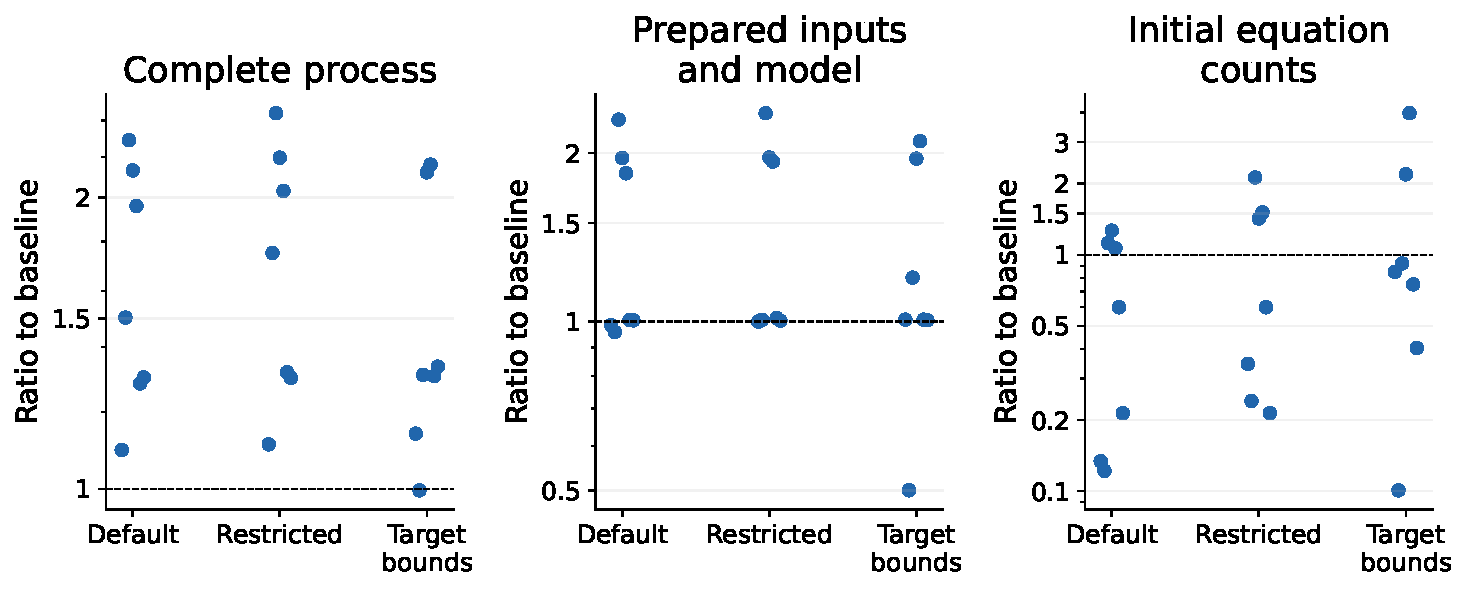
\includegraphics[width=\linewidth]{figures/kira_native_learned_seeds.pdf}
\caption{Direct native-seeding comparison on the largest frozen batches in seven independent-basis families. Ratios compare learned sector bounds with the three stated native baselines. Equation counts sum the initial system sizes that Kira reports for each attempt; internal regeneration can perform additional work.}
\label{fig:native-learned-cost}
\end{figure}

\begin{figure}[!htbp]
\centering
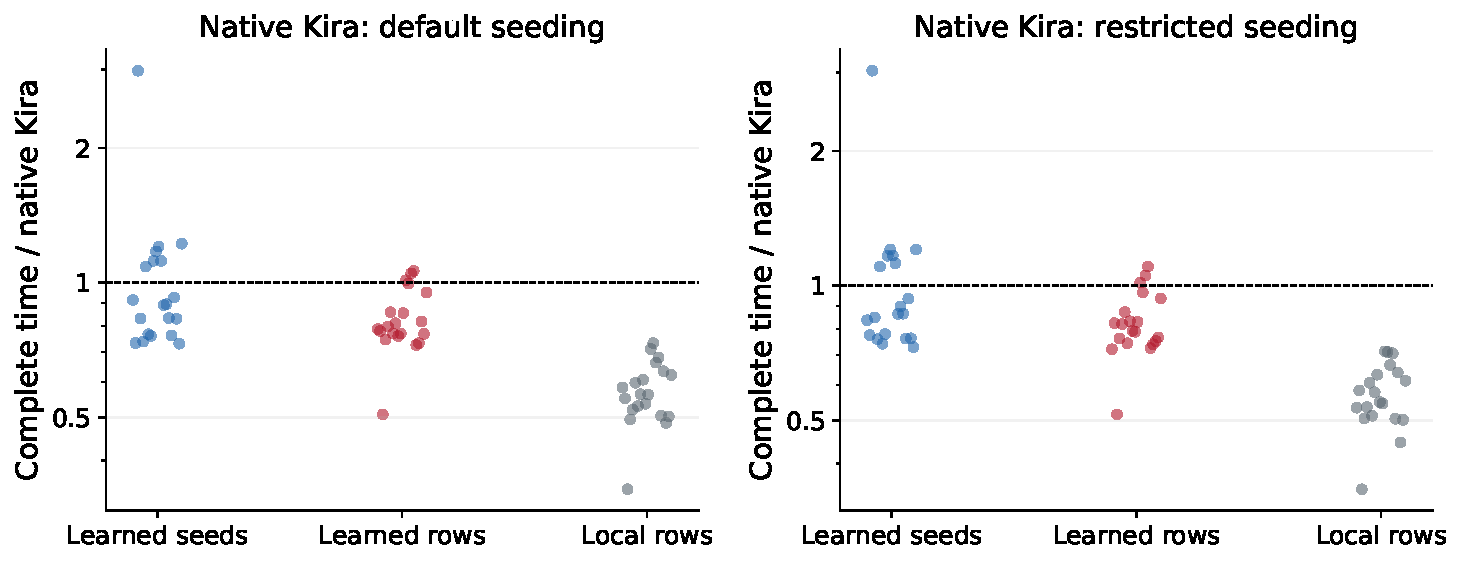
\includegraphics[width=\linewidth]{figures/kira_comparison_native.pdf}
\caption{The methods using stored identities compared with native component reduction at the same targets and master basis. Native timings include equation generation and exact combination of the component results. This comparison changes the available source representation as well as the external method, so it does not isolate the benefit of learning.}
\label{fig:native-stored-cost}
\end{figure}

\FloatBarrier
Across both comparisons, all 876 trials produced a
checked complete result within the stated bounds. The paired timing
ratios above use three completed repeats for both methods.
The recorded limits and three-repeat design bound the interpretation
of small timing differences on the shared cluster.

These results describe the implemented policies and the stated
symbolic Kira settings. The stored-pool tests reuse previously
generated identities, and the native tests measure learned sector
bounds that can include seeds beyond the model's selected set.
The row model acts on fixed source identities and target rows.
A learned policy for every pivot of Kira's evolving matrix, general
high-loop scattering families and finite-field reconstruction
requires further tests. Reduced input counts alone do not establish
a speed improvement because equation selection, model execution,
exact simplification and fallback all contribute to the total cost.
\FloatBarrier

\section{Learned Elimination Inside Kira's Evolving Matrix}
\label{sec:live-matrix}
The row comparison in Section~\ref{sec:cost-comparison} used fixed
source identities to simplify target expressions before the final Kira
call. To test the intended use inside the solver, we now apply the frozen
row model during Kira's symbolic forward elimination. The input is the
current selected IBP matrix, and every exact row update changes the state
used for the next prediction. Kira continues to generate and select
equations, preserve its integral ordering, normalize the triangular
system and perform back substitution~\cite{Kira3}.

\subsection{Choices in the current IBP matrix}
We retain the matrix notation of Eq.~\eqref{eq:reduction-action}.
At step $n$, $A^{(n)}_{rj}$ is the coefficient of integral $j$ in
identity row $r$.
Let $w(j)$ be Kira's ordering weight for integral column $j$, with larger
weights denoting integrals to eliminate earlier. The leading column of a
nonzero row $r$ and the rows with a common leading column are
\begin{equation}
 h_n(r)=\mathop{\rm arg\,max}_{j:A^{(n)}_{rj}\ne0}w(j),
 \qquad
 R_k^{(n)}=\{r:h_n(r)=k\}.
\end{equation}
At each step we take the largest-weight column that leads at least two
rows. If this column is $k_n$, the allowed choices are
\begin{equation}
 \mathcal A_n=
 \{(q,r,k_n):q,r\in R_{k_n}^{(n)},\ q\ne r\}.
 \label{eq:live-actions}
\end{equation}
Here $q$ is the source row and $r$ is the destination row.
The prescribed master columns remain protected. A proposed elimination
of a protected master, or a zero pivot at the public sampling point,
causes the learned trial to fail its interface check.

The model assigns probabilities to every pair in
Eq.~\eqref{eq:live-actions} and selects the largest score. Kira then uses
its existing symbolic update to calculate
\begin{equation}
 A^{(n+1)}_{rj}
 =A^{(n)}_{rj}
 -\frac{A^{(n)}_{rk_n}}{A^{(n)}_{qk_n}}A^{(n)}_{qj}.
 \label{eq:live-update}
\end{equation}
All these rows represent zero identities, so this operation preserves
their solution space. The new destination row has a lower leading
integral, or becomes zero and leaves the matrix. It can supply a source
row in a later step. The next prediction therefore uses the updated
identities throughout the matrix.

We use the saved 132-feature representation and model weights without
retraining. The family definition, master labels and current rows supply
the features; construction records and reference master coefficients
remain outside the predictions. Rational coefficients at the fixed
public finite-field point supply cancellation features. Kira and Fermat
perform the actual row updates with symbolic rational coefficients.
The process holding the model remains available during one forward
solve, and it receives the initial matrix followed by each changed row.
A system with no allowed row updates does not load the model.

\subsection{Matched controls and measurements}
We use the same seven families with independent master bases and 99 targets as the
native comparison in Section~\ref{sec:cost-comparison}. They include three
one-loop box profiles, a one-loop bubble, triangle and tadpole, and a
two-loop propagator. All methods use the same restricted native seed
bounds, target components, preferred masters and symbolic output checks.

Four methods distinguish the learned choice from changes needed to
measure it. Stock Kira uses the installed solver. Instrumented Kira
retains that solver's forward algorithm and records its exact updates.
The deterministic control uses the largest repeated leading integral
defined above and selects a source by Kira's row-length and integral-order
rule. A stable row identifier selects its destination. The learned
method uses the same serial schedule and selects both rows from the
allowed pairs. This control separates the model's decisions from the
effect of the new schedule. Both methods return the triangular system
to Kira for normalization and back substitution.

Each method runs three times per family on the same node, with rotated
execution order and one computation thread. Complete elapsed time
includes preparation, inference, exact algebra, target combination and
coefficient verification. We also time the forward-elimination phase
directly inside Kira and record model loading separately. The diagnostic
quantity
\begin{equation}
 T_{\mathrm{fwd,load\ excluded}}
 =T_{\mathrm{fwd}}-T_{\mathrm{model\ load}}
\end{equation}
subtracts that recorded loading interval; it retains feature construction,
scoring, communication and exact row updates. It is a timing
decomposition of these runs; a separate run with a preloaded model
has not been measured. Ratios use three-repeat medians and the
paired geometric mean of Eq.~\eqref{eq:cost-ratio}. Forward-stage ratios
include only cases with actual row updates in both methods.
The tadpole batch needs no forward row updates and does not contribute
to those phase ratios.

For each committed update, we retain the convention
$1+2n_q$, where $n_q$ is the source-row nonzero count.
This counts coefficient-field operations and excludes the internal
polynomial work in rational simplification. Elapsed time includes that
work and the candidate trial updates used to prepare features.
The tests keep the action capacity at 10,000, the matrix capacity at
10,000 rows and 250,000 nonzeros, and use bounded time and memory.
These limits bound the systems and action sets tested here.

\subsection{Exact checks and measured results}
All 84 final trials produced the prescribed symbolic master
coefficients. Independent evaluation of the archived native exports
passed 3,564 checks of target coefficients at independent sample
points, and the saved row updates passed
12,708 independent finite-field checks. The model made
1,413 choices across its repeated runs. In 465 choices,
its source row had already changed in an earlier elimination.
These records establish that the model acted on an evolving identity
matrix~\cite{KiraLiveMatrixData}.

The complete elapsed-time ratios for the learned method were
1.305 against stock Kira, 1.286 against instrumented Kira,
and 1.274 against the deterministic control. Within forward
elimination itself, the ratio against instrumented Kira was
276.149 over 6 active family batches. After subtracting the
recorded model-loading interval, the ratio was 62.270.
For those active batches, the native forward-stage medians ranged from
0.003267 to 0.076143 seconds, while the learned medians ranged from
3.061 to 6.909 seconds.

Summing one median operation count per family gives 5,771
coefficient operations for the learned method, 5,070 for
instrumented Kira and 5,097 for the deterministic control.
The corresponding learned and native row-update totals were
471 and 470.
These sums count each family once, while the independent checks above
cover all repeated runs. Figures~\ref{fig:live-times}
and~\ref{fig:live-operations} show the family-level measurements.

\begin{figure}[htbp]
\centering
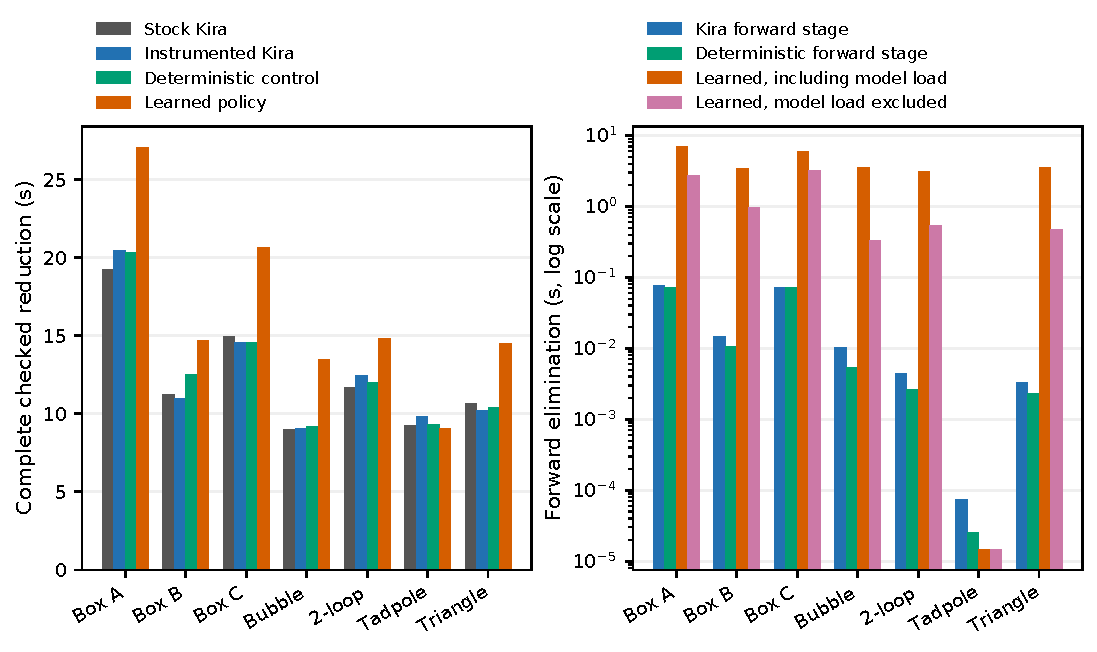
\includegraphics[width=\linewidth]{figures/live_kira_times.pdf}
\caption{Complete checked reduction time and the forward-elimination
time measured inside Kira. Bars show three-repeat medians. The forward
panel uses a logarithmic time axis and separately shows the learned time
after subtracting the recorded model-loading interval. The tadpole
case has no row updates, so its forward time measures phase overhead.
Box A, B and C denote profiles 0173, 0633 and 0156, respectively.}
\label{fig:live-times}
\end{figure}
\begin{figure}[htbp]
\centering
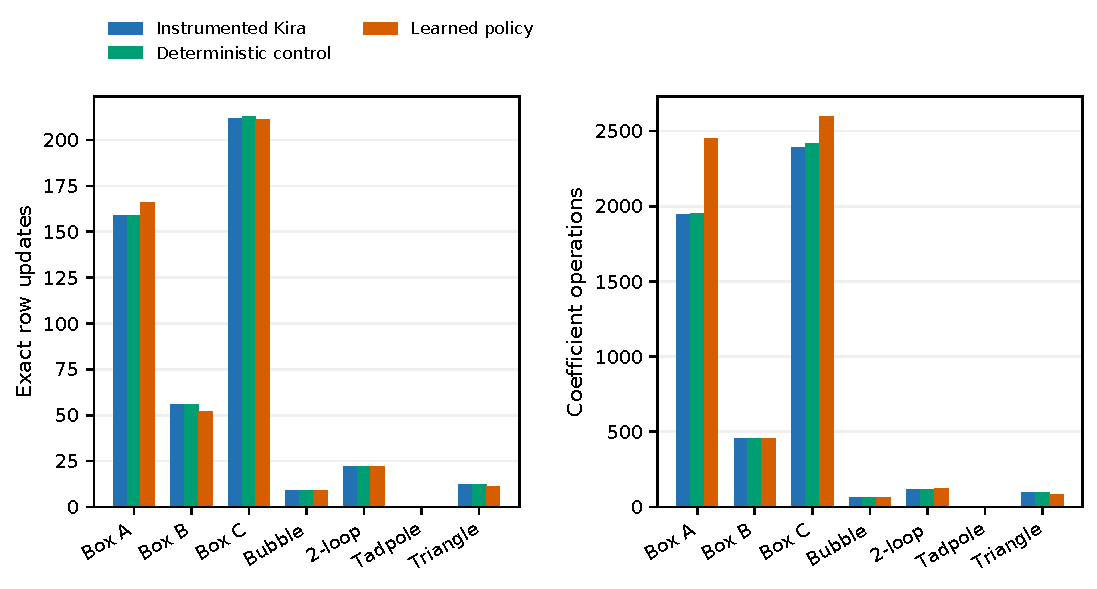
\includegraphics[width=\linewidth]{figures/live_kira_operations.pdf}
\caption{Committed row updates and coefficient-field operations for the
same evolving matrices. Each update contributes $1+2n_q$ operations.
The count excludes candidate scoring and polynomial simplification,
whose costs remain in the time measurements.}
\label{fig:live-operations}
\end{figure}
\FloatBarrier

\subsection{Implications for the proposed reduction policy}
This experiment tests learned choices inside Kira's changing selected
IBP matrix. The measured cost includes the consequences of those choices
for later rows and for the final exact reduction. The current model
increases aggregate runtime, and its summed coefficient-operation count
also exceeds the native count. Excluding model loading does not produce
a forward-elimination speedup in this comparison.

Kira's native forward phase is already short for these selected systems.
The added feature construction and scoring therefore have a small
available time budget. The model was trained on target-row reductions
with fixed source identities, so its application to changing identity
rows also tests transfer beyond those training states. The results apply
to the stated one- and two-loop families and a forward policy that
preserves Kira's integral ordering. Larger independent multiloop systems, other admissible
pivot-column choices and learned back-substitution order remain outside
the present experiment.

\section{Direct Seed Filtering and Lower-Cost Model Inference}
\label{sec:native-acceleration}
The preceding comparisons show that a learned choice must save more
algebraic work than its prediction costs. We therefore changed the
interfaces between the frozen models and Kira, and measured the complete
reductions again. The seed interface can now select individual seeds
before Kira constructs their equations. We also tested a smaller set of
row choices that follows the form of the reduction model's training
examples. The original checkpoints remain unchanged.

\subsection{Relating the predicted seeds to Kira's targets}
A stored target can contain several integrals,
\begin{equation}
 \mathcal T_\nu=\sum_{\boldsymbol a\in\mathcal J_\nu}
 c_{\nu\boldsymbol a}(\boldsymbol x,d)I_{\boldsymbol a}.
 \label{eq:accel-expression}
\end{equation}
Here $\nu$ identifies a target, $\mathcal J_\nu$ is its set of component index vectors, and
$c_{\nu\boldsymbol a}$ is the known coefficient of each component.
The native interface asks Kira to reduce these components and then
combines their reductions with exact algebra. This procedure provides
two possible inputs for the seed model: the complete expression $\mathcal T_\nu$,
or each component $I_{\boldsymbol a}$ with coefficient one.

Let $\mathcal C$ be the stored candidate seed pool and let
$p_\theta(\boldsymbol b\mid \mathcal T_\nu)$ denote the frozen model's score for
seed $\boldsymbol b$, with the family and chosen masters also supplied.
For a threshold $\tau$, the expression-based seed set is
\begin{equation}
 \widehat{\mathcal S}_{\rm expr}(\tau)
 =\bigcup_\nu\{\boldsymbol b\in\mathcal C:
             p_\theta(\boldsymbol b\mid \mathcal T_\nu)\geq\tau\}.
\end{equation}
The component-based set instead uses
\begin{equation}
 \widehat{\mathcal S}_{\rm comp}(\tau)
 =\bigcup_{\boldsymbol a\in\cup_\nu\mathcal J_\nu}
 \{\boldsymbol b\in\mathcal C:
       p_\theta(\boldsymbol b\mid I_{\boldsymbol a})\geq\tau\}.
\end{equation}
Components already in the prescribed master basis need no prediction.
A seed set sufficient for the combined expression can differ from a set
sufficient for all components separately, since terms can cancel in
Eq.~\eqref{eq:accel-expression}. Both interfaces therefore require a
check of the final expression in the prescribed master basis.

We also test a local enlargement of a predicted set,
\begin{equation}
 \mathcal N_1(\mathcal S)
 =\left\{\boldsymbol b\in\mathcal C:
   \min_{\boldsymbol a\in\mathcal S}
   \sum_{i=1}^{N}|b_i-a_i|\leq1\right\}.
 \label{eq:seed-neighbours}
\end{equation}
Here $N$ is the number of family indices. This rule adds candidate seeds
that differ by one unit in one index. It supplies nearby IBP relations
without using the reference reduction. It gives no general proof that
the set suffices.

\subsection{Filtering before equation construction}
The earlier native adapter represented predictions by sector bounds.
Those bounds include intermediate seeds even when the model omitted
them. The new interface still supplies bounds that contain the chosen
seeds, but it also checks each seed vector before Kira constructs its
IBP equations. A vector outside the selected set contributes no IBP
equations through this call. Kira retains its symmetry handling,
equation selection, exact elimination and back substitution
\cite{Kira3}. The audit records both the allowed seed vectors and the
vectors that the generator actually used.

The model scores and the reference master coefficients serve separate
purposes. Predictions use only public family, target, master-label and
candidate information. After reduction, we check whether the target
contains any integral outside the prescribed master basis. An incomplete
learned attempt triggers a standard restricted native calculation within
the remaining time allowance. The final symbolic coefficients are then
compared with the recorded exact answer. Prediction, preparation,
unsuccessful attempts, fallback, target combination and exact checks
all contribute to the measured complete time.

\subsection{Reducing prediction costs and choosing a source row}
We exported the trained weights to a NumPy implementation of the same
layers. This removes the need to import the training framework for each
reduction, and it reuses the family, master and candidate embeddings
within a target batch. On 64 development targets, the seed probabilities
differed from the original implementation by at most
$4.18\times10^{-6}$, and every decision at threshold $0.5$ agreed.
Separate bounded feature checks verified the exported row network.
These checks concern numerical inference; exact reduction still comes
from Kira and the final coefficient checks.

For the row model, we first retained the full changing-matrix interface
of Section~\ref{sec:live-matrix} with the exported network. We then
restricted each decision to a source row for one current destination.
Using the leading-column group $R_{k_n}^{(n)}$ defined there, the largest
row identifier selects the destination $r_n$, and the model scores
\begin{equation}
 \mathcal A_n^{\rm source}
 =\{(q,r_n,k_n):q\in R_{k_n}^{(n)},\ q\ne r_n\}.
\end{equation}
The feature input contains the current rows in this group, with the
destination assigned the target role. Thus the model sees one changing
destination and its allowed sources, as in its training examples.
Kira applies the selected exact update from
Eq.~\eqref{eq:live-update}. The source can itself have changed in an
earlier step. The candidate count falls from $g(g-1)$ to $g-1$ for a
group of $g$ rows, while Kira's ordering still fixes the pivot column.
If the group contains only two rows, the supplied action set has one
element, so we apply that forced action without evaluating the network.

We also implemented the source-row network inside Kira's compiled
reduction code. Each choice reads the current rows directly, samples
their rational coefficients at the fixed finite-field point and forms
the same input features. The trained weights and features retain their
single-precision values, while the compiled layer arithmetic uses
double precision. An independent implementation with the same
arithmetic precision checks the probabilities, and development tests
also compare selected sources with the original single-precision
network. This numerical prediction only selects a valid source; Kira
continues to perform the rational row update exactly.

The compiled interface removes per-choice communication with a Python
process. It retains an audit of chosen rows and their probabilities,
and the measured time includes this audit. A combined method applies
both the learned seed filter and the compiled row policy during the
same reduction. An incomplete seed attempt uses the same exact
fallback rule as the seed-only method.


This restriction changes the model's supplied state and action set.
Its purpose is to reduce prediction work and test transfer to a
closer training configuration. It does not establish an optimal
elimination order, and its benefit must be measured against Kira's
native choices.

\subsection{Checking and expanding an incomplete seed set}
In separate development trials, we tested whether Kira's initial
finite-field master check could reject an incomplete seed set before
symbolic elimination \cite{Kira3}. This check compares the integrals
left by the generated system with the prescribed master basis. A
rejected set can then be enlarged before Kira starts the more expensive
symbolic calculation. The final coefficients still require exact
checks, since a numerical rank check alone does not prove the full
symbolic reduction. We retained the frozen policies in the reserved
comparison while testing these extensions.

For the first expansion rule, we rank each candidate seed by its
largest model score across the supplied expressions,
\begin{equation}
 Q_\theta(\boldsymbol b)
 =\max_\nu p_\theta(\boldsymbol b\mid\mathcal T_\nu).
\end{equation}
We begin with the first $k_0=32$ seeds and, after a rejected master
check, increase the budget according to
\begin{equation}
 k_{j+1}=\min(2k_j,|\mathcal C|).
\end{equation}
Here $j$ is the number of completed expansion steps and $\mathcal C$
is the candidate pool defined above. A control ranks seeds by their
smallest index distance to a component of a target expression, and
uses the same budget rule. The full candidate pool and restricted
native seeding provide two further controls.

A second rule begins with 64 seeds and uses the additional integrals
returned by the master check as new model inputs. Each such input
contains one integral with coefficient one. We add its four
highest-ranked unused candidates and repeat the check, using the full
pool after five rejected checks. A distance-based control applies the
same expansion to the same additional integrals. These checks require
every component to reduce in the prescribed basis, which can be
stricter than reducing the complete expression when terms cancel.

The 26 development trials gave 23 exact completions and three bounded
incomplete calculations. The latter used 64-target batches and affected
the native control and both learned variants in the initial check
experiment. All completed outputs passed 1104 independent
finite-field target checks. Across four complete 16-target comparisons,
the doubling rule with learned ranking took 1.022--1.422 times the
native control's complete time. In the subsequent residual-driven
trial, learned ranking reached a complete basis with 71 seeds,
while the distance control used 121. Its complete-time ratio
against native seeding was 0.996. These are single development
measurements; they do not establish a repeatable speedup for either
expansion strategy \cite{KiraNativeAccelerationData}.


\subsection{Development, validation and reserved comparisons}
We selected family instances before the new timing comparisons.
Development and adapter-validation instances use separate kinematic
groups from the original model-training partition. The reserved
cost-test instances come from the original test partition, and their
kinematic groups exclude every box group in the earlier cost comparison.
The network weights remain fixed throughout this selection.
The adapter-validation families belong to the original training
partition, so this stage selects an interface configuration and does
not measure generalization of the network itself. We performed
development comparisons on three of the reserved development
instances, selected the seed configuration on six validation instances
and then froze the policy before testing twelve instances from six
reserved kinematic groups.

All new native cases use symbolic reduction of one-loop box families
with independent propagator bases. Each case uses the same target expressions and master
basis for every method. Controls include restricted native seed bounds,
bounds taken directly from target indices, and the full stored candidate
pool with the individual-seed filter. These controls separate the
learned selection from changes to seed bounds or equation generation.

Every trial uses one computation thread with explicit time, memory and
scratch limits. We increased the array allowance from two simultaneous
jobs to four and then eight after checking the available node memory and project
storage. This changed the scheduling of independent trials while
preserving their individual resource limits and frozen policies. Methods run in rotated order on the same node for each
family and target-batch size. The retained-evidence limit interrupted some batches before a new trial could start; after lossless archive recompression, we resumed the missing trials on their original nodes and retained every completed observation. Every reserved method receives the same
initial 160-second native calculation allowance within a 180-second
complete-process limit. The memory and scratch limits are also the
same. We retain failed trials and report their completion status.
The validation rule assigns the 180-second total cap to an incomplete
trial when choosing the learned seed configuration. This capped score
is a selection rule; it is not a measured time for a completed
reduction. The reserved comparison uses the frozen configuration,
five repetitions and batches of 16 and 64 stored target expressions.
After an unsuccessful attempt, the remaining identical repetitions for
that method and batch are marked as skipped. Skipped repetitions receive
no measured time. Timing ratios require five successful repeats for both
methods, while completion and failure counts retain every attempted
case.

\subsection{Reserved results and exact checks}

\label{sec:acceleration-results}

The frozen comparison contains 720 planned records across twelve family instances, two target-batch sizes, six methods and five repetitions. We executed 616 trials and obtained 590 exact completions; the remaining 26 executed trials exceeded a resource limit or failed to complete. The early-stop rule left 104 repetitions unexecuted. These skipped records contain no timing measurement. The retained inputs, policy choices, successful reductions and failure records accompany the data release~\cite{KiraNativeAccelerationData}.

Validation selected the complete target expression with threshold $\tau=0.01$. This configuration and both trained checkpoints remained fixed during the reserved tests. Each method used the same master basis and targets in a batch.

For the three controls, restricted native Kira produced 105 exact completions, 3 failed trials and 12 skipped repetitions, the target-bound control produced 100 exact completions, 4 failed trials and 16 skipped repetitions, and the full candidate-pool control produced 105 exact completions, 3 failed trials and 12 skipped repetitions. These counts describe the bounded experiment and do not measure whether an unlimited calculation would complete.

Successful restricted-native trials took 10.54--112.46 seconds for the complete checked calculation. This range includes different family instances, target-batch sizes and CPU models. The paired ratios compare methods on the same node within each batch.

For the learned methods, the learned seed filter produced 100 exact completions, 4 failed trials and 16 skipped repetitions, the compiled row policy produced 105 exact completions, 3 failed trials and 12 skipped repetitions, and the combined method produced 75 exact completions, 9 failed trials and 36 skipped repetitions. Completed seed and combined trials used the standard fallback 30 and 50 times, respectively.

Every completed final expression matched its recorded rational master coefficients. The independent audit performed 67,920 additional master-coefficient sample checks and 65,355 exact-row sample checks. It checked 11,405 compiled model choices and 10,380 forced source actions. Trace checks cover completed native attempts; 55 failed attempts had incomplete traces. The final coefficient checks still apply to any successful fallback. Input and checkpoint hashes agree with the values frozen before testing.

\subsection{Complete reduction time and algebraic work}

For each family and batch size, we take the median of five successful repetitions. We then form the ratio of learned time to control time and report the geometric mean across complete paired batches. A ratio below one means a lower measured time. We resample complete kinematic groups 10,000 times to obtain descriptive 95\% intervals, keeping related profiles and batch sizes together. These intervals describe the completed subset of this small collection; failed and skipped trials remain in the completion counts above.

Restricted native Kira completed all five repetitions in 1 batches where the learned seed filter did not, while the learned seed filter completed all five repetitions in 0 batches where that control did not.

The learned seed filter has a complete-time ratio of 1.295 (descriptive 95\% interval 1.156--1.542; 20 batches) against restricted native Kira. Its native-calculation subtotal, including seed prediction when used, has ratio 1.400 (descriptive 95\% interval 1.201--1.816; 20 batches). The subtotal excludes input preparation, final target combination and verification, which remain included in the complete time.

Restricted native Kira completed all five repetitions in 0 batches where the compiled row policy did not, while the compiled row policy completed all five repetitions in 0 batches where that control did not.

The compiled row policy has a complete-time ratio of 1.024 (descriptive 95\% interval 0.998--1.053; 21 batches) against restricted native Kira. Its native-calculation subtotal, including seed prediction when used, has ratio 1.025 (descriptive 95\% interval 1.001--1.078; 17 batches). The subtotal excludes input preparation, final target combination and verification, which remain included in the complete time.

Restricted native Kira completed all five repetitions in 6 batches where the combined method did not, while the combined method completed all five repetitions in 0 batches where that control did not.

The combined method has a complete-time ratio of 1.983 (descriptive 95\% interval 1.575--2.476; 15 batches) against restricted native Kira. Its native-calculation subtotal, including seed prediction when used, has ratio 2.289 (descriptive 95\% interval 1.247--3.673; 8 batches). The subtotal excludes input preparation, final target combination and verification, which remain included in the complete time.

Against the target-bound control, complete-time ratios are 0.902 (descriptive 95\% interval 0.711--1.163; 20 batches), 0.712 (descriptive 95\% interval 0.597--0.864; 20 batches), 1.415 (descriptive 95\% interval 0.902--2.160; 14 batches), in seed, row and combined order. Against the full candidate-pool control, the corresponding ratios are 1.317 (descriptive 95\% interval 1.167--1.569; 20 batches), 1.040 (descriptive 95\% interval 1.016--1.061; 21 batches), 2.028 (descriptive 95\% interval 1.565--2.616; 15 batches). Each ratio uses its own complete paired cohort, so comparisons with different failure patterns can contain different batches.

\begin{figure}[htbp]
\centering
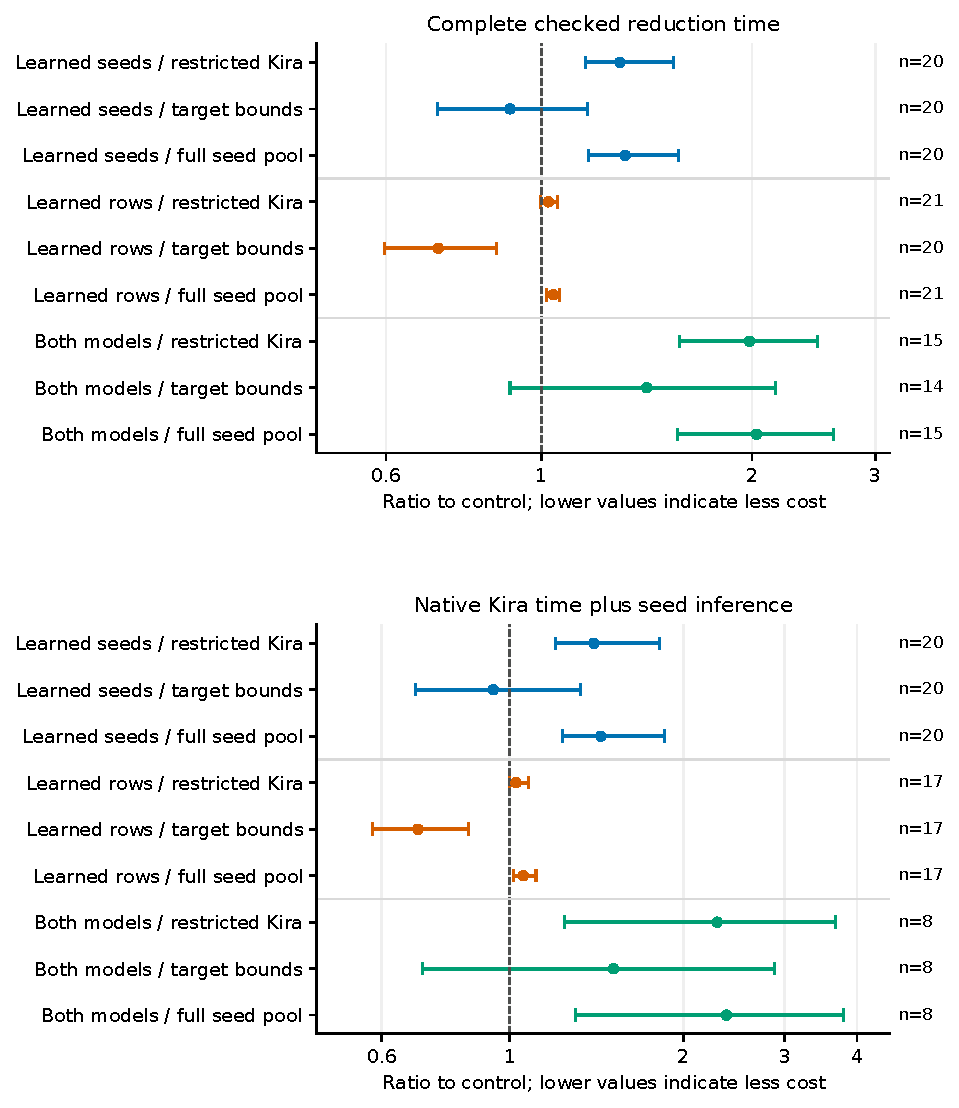
\includegraphics[width=\linewidth]{figures/native_acceleration_times.pdf}
\caption{Learned-to-control time ratios in the reserved native comparison.
The upper panel includes the complete checked reduction, and the lower panel
shows the native subprocess subtotal plus seed prediction. Points show
geometric mean ratios and lines show descriptive intervals obtained by
resampling kinematic groups. The label $n$ gives the number of paired
batches with five successful repeats for both methods.}
\label{fig:native-acceleration-time}
\end{figure}

The learned seed filter has a generated-equation ratio of 0.168 (descriptive 95\% interval 0.097--0.294; 20 batches), a selected-equation ratio of 0.982 (descriptive 95\% interval 0.797--1.205; 20 batches) and a forward-update ratio of 3.575 (descriptive 95\% interval 2.647--5.211; 20 batches) against restricted native Kira. These are counters from the native reduction passes, including completed fallback passes.

The compiled row policy has a generated-equation ratio of 1.141 (descriptive 95\% interval 1.032--1.275; 21 batches), a selected-equation ratio of 1.141 (descriptive 95\% interval 1.032--1.275; 21 batches) and a forward-update ratio of 0.905 (descriptive 95\% interval 0.840--0.972; 17 batches) against restricted native Kira. These are counters from the native reduction passes, including completed fallback passes.

The combined method has a generated-equation ratio of 0.462 (descriptive 95\% interval 0.254--0.745; 15 batches), a selected-equation ratio of 1.341 (descriptive 95\% interval 1.080--1.582; 15 batches) and a forward-update ratio of 2.363 (descriptive 95\% interval 1.041--4.534; 8 batches) against restricted native Kira. These are counters from the native reduction passes, including completed fallback passes.

Generation counters count equations reported in successive generation passes and can include repeated equations. A forward update is one committed elimination step; this count does not measure every polynomial or rational-function operation. Failed attempts can have truncated work counters, so the complete time and completion status remain the primary measures.

\begin{figure}[htbp]
\centering
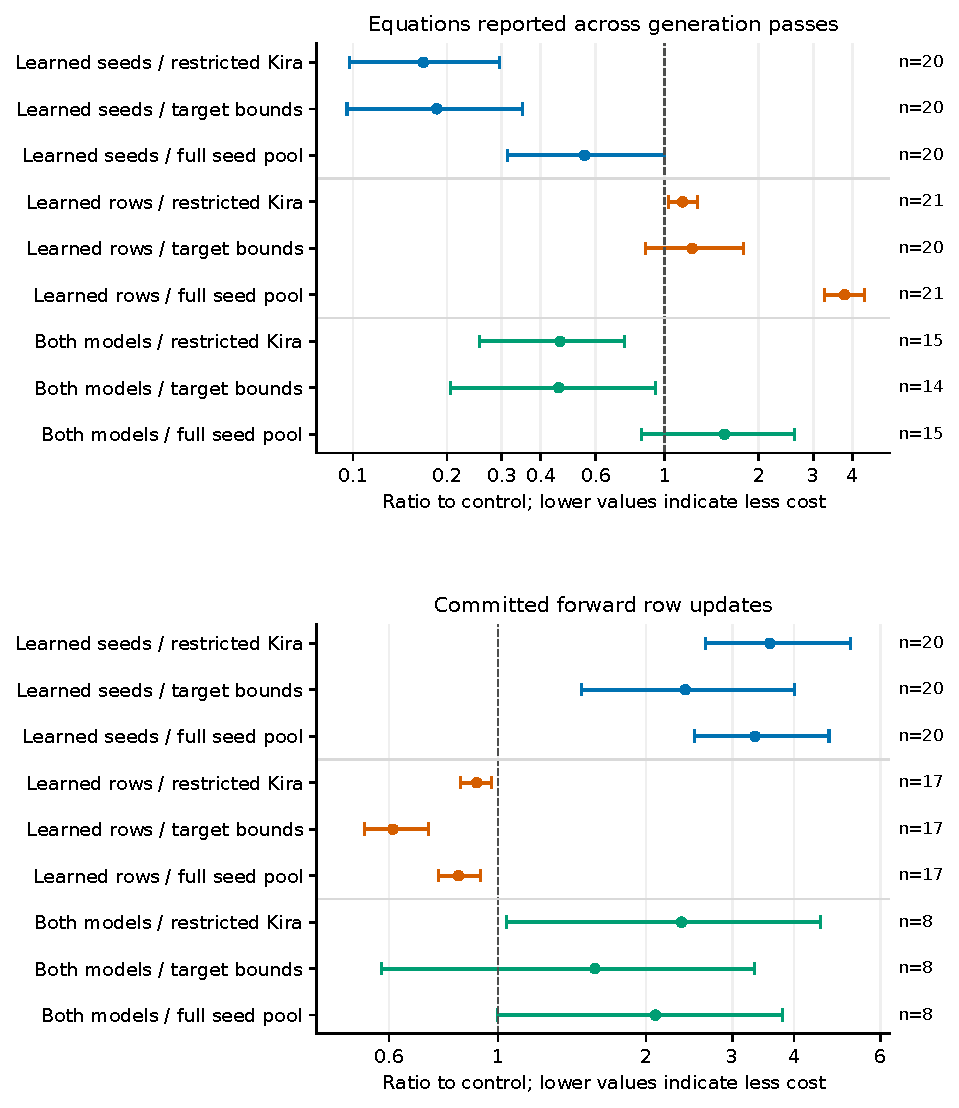
\includegraphics[width=\linewidth]{figures/native_acceleration_work.pdf}
\caption{Generated-equation and forward-update ratios on complete paired
batches. The controls and cohort labels follow
Fig.~\ref{fig:native-acceleration-time}. These counters measure reported
generation work and committed updates, while symbolic coefficient
complexity can change the cost of each update.}
\label{fig:native-acceleration-work}
\end{figure}
\FloatBarrier

\subsection{Numerical inference and scope of the result}

The compiled-model development audit checked 256 action feature vectors and 2,247 sampled coefficients. The maximum feature difference was 0, and the largest probability difference from the independent double-precision calculation was $1.41\times10^{-13}$. All selected sources agreed with the original single-precision model in these development trials. The separate maximum probability difference from that original arithmetic was $1.6\times10^{-05}$.

The largest sampled process-tree memory was 0.506 GB, and the largest trial scratch directory was 49.29 MB. The bounded runs kept their scientific records and model files on Hoffman; the report contains the derived plots and results.

The complete paired comparisons do not show a lower aggregate runtime than restricted native Kira for these learned methods. Lower inference costs alone do not ensure that the chosen seeds and rows save enough algebraic work. The new native tests cover one-loop boxes and do not establish performance on independent high-loop scattering families. The existing weights were trained to recover recorded seed sets and row choices, and Section~\ref{sec:complete-multiloop} reports a separate cost-trained policy on native Kira trajectories.

\subsection{Transfer to a two-loop propagator family}
We also applied the unchanged interfaces to the massless two-loop
propagator family used in the earlier cost comparisons. Its five
independent family indices fit the compiled row interface. We fixed
two batches of 16 and 64 stored target expressions and all policies
before this transfer calculation. Each method uses five rotated
repetitions, the same master basis and the same time and memory limits.
Storage-interrupted trials resume on their original node, with earlier
observations preserved. Because this family appeared in earlier
comparisons, this experiment measures transfer of the revised
implementation and does not establish generalization to a newly unseen
family.

Alongside native seeding and the full candidate pool, we include a
deterministic source-row control using the same compiled reduction
structure. This control selects a source by row length and integral ordering
within the same changing leading-column group. Comparing the learned row policy
with this control separates the source choice from changes to the
compiled reduction structure. Every completed reduction receives the
same exact coefficient check and an independent finite-field check.

The transfer experiment contains 60 measured trials among 60 planned records, with 60 exact completions. The independent audit performed 7,200 target-coefficient checks and 2,355 row-update checks.

For 16 targets, the native control's median complete time was $12.003$ seconds. The learned seed filter gave a time ratio of $0.992$ with descriptive interval $[0.962,1.030]$; the learned source-row policy gave a time ratio of $0.991$ with descriptive interval $[0.984,1.022]$; the combined policy gave a time ratio of $0.976$ with descriptive interval $[0.961,0.996]$. In the matched controls, the learned seed filter relative to the full pool had ratio $1.051$ with interval $[1.024,1.072]$ and the learned source choice relative to the deterministic compiled control had ratio $0.987$ with interval $[0.979,1.034]$.

For 64 targets, the native control's median complete time was $12.770$ seconds. The learned seed filter gave a time ratio of $1.758$ with descriptive interval $[1.744,1.777]$; the learned source-row policy gave a time ratio of $0.976$ with descriptive interval $[0.964,0.992]$; the combined policy gave a time ratio of $1.755$ with descriptive interval $[1.740,1.777]$. In the matched controls, the learned seed filter relative to the full pool had ratio $1.907$ with interval $[1.880,1.920]$ and the learned source choice relative to the deterministic compiled control had ratio $0.987$ with interval $[0.952,1.012]$.


The compiled learned-row pipeline reduced the median complete time for
64 targets from 12.770 to 12.460 seconds, a measured reduction of
2.4\%. Its ratio against the deterministic compiled control has an
interval that includes one, so this experiment does not resolve a
benefit caused by the learned source choice itself. The full-pool
control was faster, at 11.773 seconds. For 16 targets, the combined
pipeline reduced the native median by 2.4\%, but the full-pool control
again completed sooner. For 64 targets, every learned-seed and combined
trial required fallback, whose cost is included in the reported time.
These observations establish limited gains relative to the stated
native baseline and also identify stronger deterministic controls.


Figure~\ref{fig:native-transfer} shows all complete paired comparisons.
A ratio below one denotes a lower median complete time. The intervals
come from 10,000 paired resamples of the five repetitions and describe
repeat-to-repeat variation within this one family. They do not measure
uncertainty across different integral families. Incomplete pairs remain
in the completion counts and receive no timing ratio
\cite{KiraNativeAccelerationData}.

\begin{figure}[htbp]
 \centering
 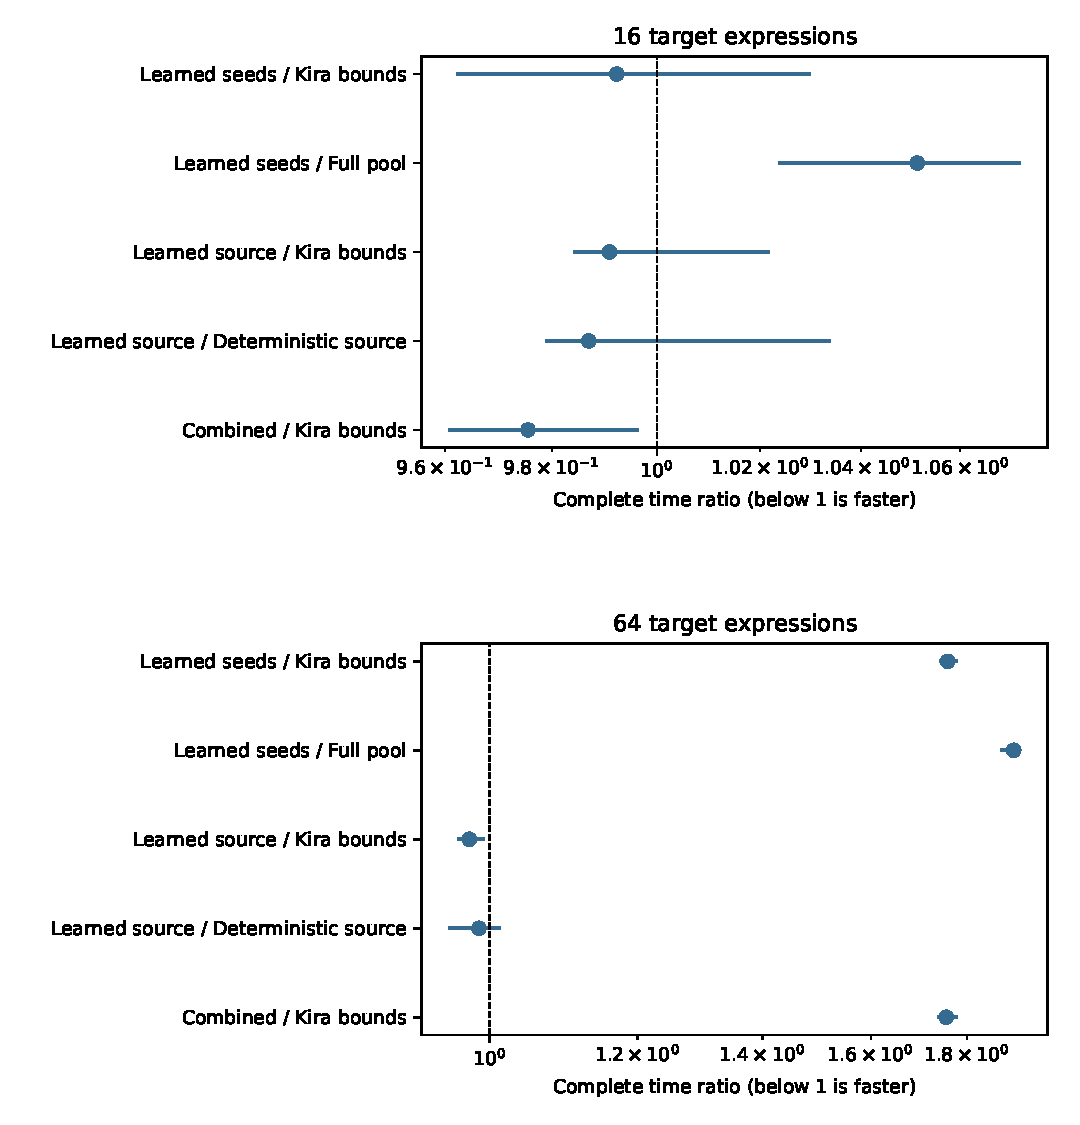
\includegraphics[width=\textwidth]{figures/native_transfer_times.pdf}
 \caption{Complete-time ratios in the two-loop transfer comparison for
 16 targets (upper panel) and 64 targets (lower panel). Points show
 ratios of five-repeat medians, and bars show descriptive paired-repeat
 intervals. All times include prediction, target preparation, exact
 reduction, combination, checks and any required fallback.}
 \label{fig:native-transfer}
\end{figure}


\subsection{Applying the seed model to complete target expressions}
The native interface reduces each component of
Eq.~\eqref{eq:accel-expression} before combining the result. We also
applied the fast seed model directly to that complete expression,
using Kira's supplied-equation mode. This tests the form of the target
used to train the seed model and allows cancellations between its
components during the reduction.

Let $\mathcal E_{\boldsymbol b}$ be the stored IBP identities generated
from candidate seed $\boldsymbol b$, and let
$\mathcal E_{\rm bg}$ contain the stored symmetry and other background
identities. The selected equation set is
\begin{equation}
 \mathcal E(\mathcal S)=\mathcal E_{\rm bg}\cup
       \bigcup_{\boldsymbol b\in\mathcal S}\mathcal E_{\boldsymbol b}.
\end{equation}
For each requested expression, we add its defining relation
\begin{equation}
 \mathcal T_\nu-
 \sum_{\boldsymbol a\in\mathcal J_\nu}
 c_{\nu\boldsymbol a}I_{\boldsymbol a}=0.
\end{equation}
Kira eliminates the supplied system with the target expressions ordered
above their component integrals and the prescribed masters preferred
at the end of the ordering. It therefore obtains the master expansion
of $\mathcal T_\nu$ in one exact solve. The same public identity pool,
target definitions and master basis enter every compared method.

The model takes the union of candidates whose score reaches
$\tau=0.01$, using the unchanged weights and the fast inference
implementation. We tested this set both with and without an early
finite-field master check. An incomplete selected system triggers a
full-pool calculation within the remaining time allowance. The early
check compares the remaining integrals with the prescribed master
basis; exact final coefficient checks still determine whether the requested reductions
agree with their recorded answers. A global master check can require
more relations than a particular target combination needs.

These calculations begin with stored IBP identities, whose prior
generation cost is excluded for every method. The measured complete
time includes loading those inputs, prediction, equation selection and
export, Kira's exact calculation, admission checks when used, failed
attempts, fallback and final verification. Thus the result concerns
repeated reduction from a common identity pool. It does not measure
native generation of a new family's equations.


The separate development and adapter-validation collection contains 80 trials, with 74 exact completions and 6 incomplete calculations. Independent checks evaluated 2,013 target coefficients at stored finite-field points. The six adapter-validation family instances belong to the original training partition and use two batch sizes, one and sixteen targets. We retained every measured cost and selected a learned interface only when its geometric mean complete-time ratio to the full-pool control was below one and it preserved every control completion.

The validation ratio without the early master check was 1.113 across 11 complete paired batches. The full-pool control completed 0 additional batches that this learned interface did not complete. These single validation measurements select the interface and do not establish a repeatable timing gain.

The validation ratio with the early master check was 0.930 across 11 complete paired batches. The full-pool control completed 0 additional batches that this learned interface did not complete. These single validation measurements select the interface and do not establish a repeatable timing gain.

\subsection{Reserved tests of complete-expression reduction}

Validation selected the early master check. We froze this choice before applying it to the twelve original-held-out box instances used in the native comparison. The network weights and threshold remain fixed. Each instance supplies batches of one and sixteen target expressions, with five rotated repetitions per method on the same node. These are reused physical families and constructed targets; the new comparison tests the revised interface on original-held-out model data.

The controls use the full stored identity pool and a fixed set of 64 seeds ranked by their smallest index distance to any target component. The distance control uses the same exact reduction and full-pool fallback as the learned method. This first distance control proceeds directly to symbolic elimination, while the selected learned method uses the early master check. Their time ratio therefore includes both seed selection and the difference in admission checks.

The frozen plan contains 360 records. We executed 348 trials and obtained 345 exact completions; 3 measured trials failed to complete within the bounds, and 12 remaining repeats were skipped after an earlier failure. Every completed master expansion matched its exact reference, and the independent audit checked 8,460 target coefficients directly against the exported Kira reductions. Skipped repetitions have no assigned runtime.

The learned interface produced 115 exact completions, 1 failed trial and 4 skipped repeats. Completed trials used fallback 25 times.

The full-pool control produced 115 exact completions, 1 failed trial and 4 skipped repeats. Completed trials used fallback 0 times.

The distance control produced 115 exact completions, 1 failed trial and 4 skipped repeats. Completed trials used fallback 55 times.

We form a median from five successful repetitions for each method and batch, and take geometric mean ratios over complete paired batches. Descriptive 95\% intervals resample the six kinematic groups 10,000 times, preserving the relationship between profiles and batch sizes. Completion losses remain separate from these ratios.

The learned interface has a complete-time ratio of 0.944 against the full-pool control, with descriptive interval $[0.863,1.042]$ across 23 paired batches. The control completed all repeats in 0 additional batches, and the learned method completed all repeats in 0 additional batches.

The learned interface has a complete-time ratio of 0.604 against the distance control, with descriptive interval $[0.534,0.678]$ across 23 paired batches. The control completed all repeats in 0 additional batches, and the learned method completed all repeats in 0 additional batches.

The observed geometric mean complete time is 5.6\% lower than the full-pool Kira control on batches where both methods completed all five repetitions. Because the descriptive interval includes one, the aggregate timing gain across both batch sizes remains uncertain. The result applies to these constructed target expressions and their existing identity pools; it does not establish a speedup for general multiloop amplitude reductions \cite{KiraNativeAccelerationData}.

\begin{figure}[htbp]
\centering
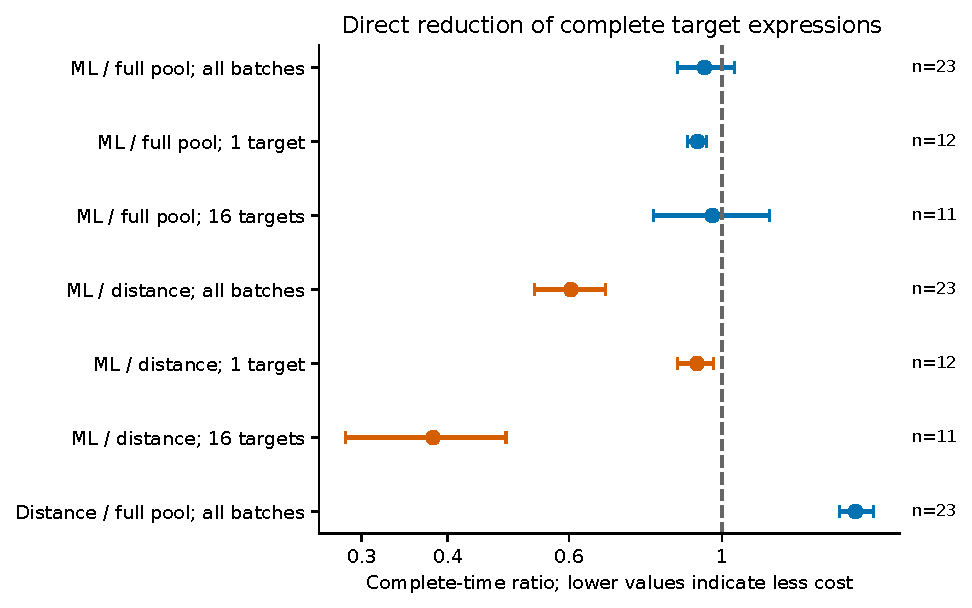
\includegraphics[width=\linewidth]{figures/whole_expression_times.pdf}
\caption{Complete-time ratios for direct reduction of complete target
expressions. Points show geometric means of five-repeat median ratios,
and intervals resample kinematic groups. The label $n$ gives the
number of complete paired batches. Failed and skipped trials remain
in the completion counts.}
\label{fig:whole-expression-time}
\end{figure}
\FloatBarrier



\subsection{Using the same master check for both seed selectors}
The preceding distance control enters symbolic elimination directly,
while the learned method first checks the selected master basis.
To compare seed choices under the same admission procedure, we fixed
a second confirmation in which both selected sets receive the same
early check and full-pool fallback. The learned scores, threshold,
distance rule, twelve family instances and target batches stay
unchanged. The full-pool Kira control again uses its standard
supplied-equation reduction. We retained every measurement in the
first comparison.

Each method again uses five rotated repetitions on the same node
within a family and batch. This new comparison contains independent
timing repetitions of the same physical cases, so it checks the effect
of matching the admission procedure and does not introduce new
integral families. Complete times and descriptive intervals follow
the definitions in the preceding subsection.


The comparison with the same early check contains 360 records, of which 348 are measured trials. It produced 345 exact completions, 3 incomplete measured trials and 12 skipped repetitions. Independent checks evaluated 8,460 target coefficients against the raw Kira exports. All completed reductions matched their exact reference coefficients.

The learned method completed 115 trials exactly, with 1 failed trial and 4 skipped repetitions. Its completed trials required fallback 25 times.

The full-pool control completed 115 trials exactly, with 1 failed trial and 4 skipped repetitions. Its completed trials required fallback 0 times.

The distance control with the early check completed 115 trials exactly, with 1 failed trial and 4 skipped repetitions. Its completed trials required fallback 55 times.

Across both batch sizes, the learned complete-time ratio to the full-pool control is 0.932, with descriptive interval $[0.845,1.031]$ across 23 paired batches. The control completed 0 additional batches, while the learned method completed 0 additional batches.

For batches of 1 target, the learned complete-time ratio to the full-pool control is 0.914, with descriptive interval $[0.871,0.958]$ across 12 paired batches. The control completed 0 additional batches, while the learned method completed 0 additional batches.

For batches of 16 targets, the learned complete-time ratio to the full-pool control is 0.952, with descriptive interval $[0.772,1.148]$ across 11 paired batches. The control completed 0 additional batches, while the learned method completed 0 additional batches.

Across both batch sizes, the learned complete-time ratio to the distance control with the same early check is 0.925, with descriptive interval $[0.848,1.024]$ across 23 paired batches. The control completed 0 additional batches, while the learned method completed 0 additional batches.

For batches of 1 target, the learned complete-time ratio to the distance control with the same early check is 0.913, with descriptive interval $[0.855,0.972]$ across 12 paired batches. The control completed 0 additional batches, while the learned method completed 0 additional batches.

For batches of 16 targets, the learned complete-time ratio to the distance control with the same early check is 0.939, with descriptive interval $[0.764,1.136]$ across 11 paired batches. The control completed 0 additional batches, while the learned method completed 0 additional batches.

For the predefined single-target comparison, the learned method reduced geometric mean complete time by 8.6\% relative to the full pool and by 8.7\% relative to the distance rule with the same early check. Both descriptive intervals lie below one, and every method completed all five repeats for all twelve instances. The first confirmation gave a 7.8\% reduction relative to the full pool for this batch size. These results support a repeated gain for one constructed target expression at a time in this stored-identity setting. The sixteen-target intervals include one, so that batch size does not establish a consistent gain. The geometric means of the twelve per-family median complete times were 5.478 seconds for the full pool and 5.005 seconds for the learned method.

The learned workflow has an observed 6.8\% lower geometric mean complete time than the full-pool Kira control on batches where both methods completed all five repetitions. Because the descriptive interval includes one, the aggregate timing gain across both batch sizes remains uncertain. These conclusions concern reduction from the supplied identity pools and the tested constructed target expressions. Native equation generation, arbitrary scattering amplitudes and larger independent multiloop families remain outside this result \cite{KiraNativeAccelerationData}.

\begin{figure}[htbp]
\centering
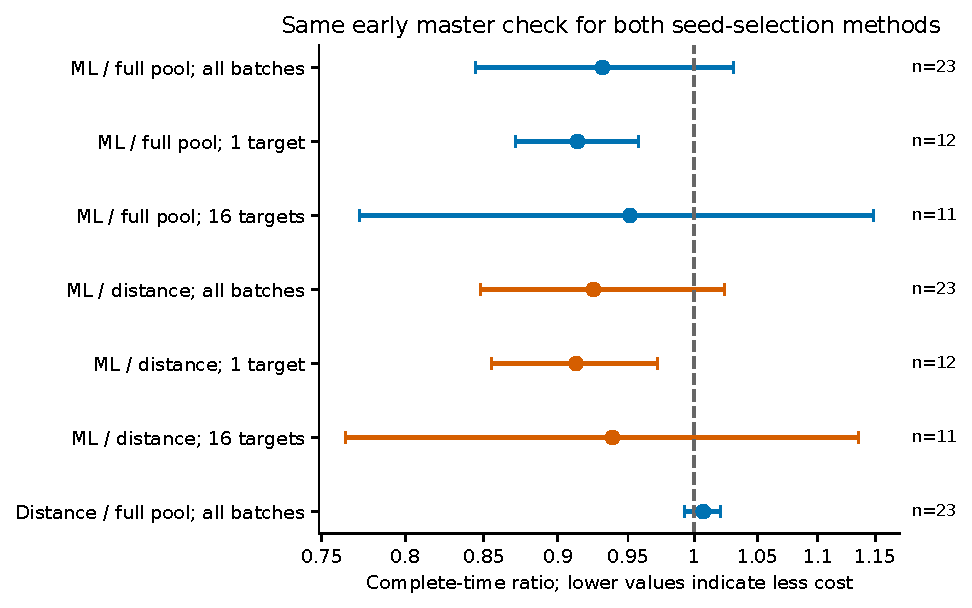
\includegraphics[width=\linewidth]{figures/whole_expression_matched_times.pdf}
\caption{Complete-time ratios with the same early master check for
learned and distance-selected seeds. Points show geometric means
of five-repeat median ratios, intervals resample kinematic groups,
and $n$ gives the number of complete paired batches. The full-pool
control uses standard supplied-equation Kira reduction.}
\label{fig:whole-expression-matched}
\end{figure}
\FloatBarrier



\subsection{Reducing fixed waits in the exact reduction workflow}
The preceding comparisons show that the cost of using the seed model
depends on the full reduction workflow. Inspection of the Kira version
used here found a fixed one-second wait each time the program closed
a Fermat process. Fermat performs exact rational-function arithmetic,
and this wait occurs after the interface sends its exit command and
closes its pipes. The program then checks whether the child has exited
and forces termination if it is still running.

We replaced this fixed wait with repeated checks of the same child
process at two-millisecond intervals. The modified interface returns
as soon as it observes the exit and retains a one-second grace period
before forced termination. It also handles interrupted checks and
already reaped children. Tests checked that the arithmetic process exits normally or reaches
the existing termination limit. We built this change separately from the original
Kira executable. The symbolic elimination code, rational coefficients,
model weights and seed threshold remain unchanged
\cite{KiraResponsiveExitData}.

This change acts on a distinct part of the complete cost,
\begin{equation}
 T_{\rm total}=T_{\rm input}+T_{\rm model}+T_{\rm algebra}
             +T_{\rm exit}+T_{\rm check}.
\end{equation}
Here $T_{\rm input}$ includes loading and equation preparation,
$T_{\rm model}$ includes loading the seed model and computing its scores,
$T_{\rm algebra}$ is the time spent in exact reduction,
$T_{\rm exit}$ is the time needed to close its arithmetic processes,
and $T_{\rm check}$ is the final coefficient-verification time.
Failed attempts and fallback contribute to the corresponding terms.
Removing the fixed part of $T_{\rm exit}$ can improve a short reduction
without changing its algebraic operation count.

\subsubsection{Separating shutdown costs from learned seed selection}
We compare four complete workflows: the original Kira with all supplied
equations, the original Kira with learned seeds, the modified Kira with
all supplied equations, and the modified Kira with learned seeds.
The learned workflows use the existing model, the fixed threshold
$0.01$, the early master check and the same full-pool fallback.
Thus, comparing the two learned workflows isolates the shutdown change,
while comparing learned selection with the full pool within the modified
Kira measures the remaining benefit of that seed-selection workflow.

Development uses three instances from the original training partition.
The reserved comparison uses twelve other one-loop box instances in
six original-test kinematic groups that were absent from all earlier
box cost-test groups. Each instance has batches of one and sixteen
constructed targets, and each workflow receives five rotated repetitions
on the same node for that instance and batch size. We fixed the cases
before timing the change and froze the executable, code, model and
scientific inputs before the reserved runs.

Every measured time includes a fresh process start, input preparation,
model inference where applicable, exact Kira reduction, failed attempts,
fallback and exact coefficient checks. The prior generation of the shared
IBP identity pools is outside all four methods. Each trial uses one thread,
a 180-second complete-process cap, a 1.7 GB process-tree memory limit and
32 MiB of temporary storage. The array began with two simultaneous trials and increased to three
and then six after memory and storage checks. The individual limits,
targets, models and calculation code stayed fixed.
After a failed measured attempt, further identical repetitions are
marked as skipped and receive no measured time.

The timing comparison uses the median of five successful repetitions
for each method and batch. We form the geometric mean of their paired
time ratios and obtain descriptive 95\% intervals by resampling entire
kinematic groups 10,000 times. These intervals describe the completed
subset, and the separate completion counts retain every planned case.

Development produced 10 exact completions from 12 measured trials. The reserved comparison contains 480 planned records, 416 measured trials and 400 exact completions. Independent checks compared 8,850 sampled master-coefficient vectors with the raw Kira exports. Every completed reduction matched its exact reference coefficients.

Each workflow completed 100 trials exactly and recorded 4 failed attempts and 16 skipped repetitions. Each learned workflow used full-pool fallback 10 times among its completed trials. The paired comparisons below identify the successful batch sets.

\subsubsection{Measured complete-time changes}
For one target at a time, the modified learned workflow has a complete-time ratio of 0.385, with a descriptive 95\% interval $[0.342,0.453]$ from 12 complete paired batches relative to the original learned workflow. The corresponding geometric mean times are 5.528 and 2.126 seconds, a 61.5\% reduction. For sixteen targets, the ratio to the original learned workflow is 0.686, with a descriptive 95\% interval $[0.540,0.844]$ from 8 complete paired batches.

With the responsive shutdown active in both methods, learned seed selection has a one-target complete-time ratio of 0.690, with a descriptive 95\% interval $[0.424,0.931]$ from 11 complete paired batches relative to the full pool. The corresponding sixteen-target ratio is 0.983, with a descriptive 95\% interval $[0.915,1.063]$ from 8 complete paired batches. The one-target comparison therefore retains a measured 31.0\% reduction from the learned seed workflow after the shutdown improvement. The sixteen-target interval includes one, so a consistent additional benefit remains unresolved for that batch size.

The modified learned workflow has a one-target complete-time ratio of 0.282, with a descriptive 95\% interval $[0.199,0.349]$ from 11 complete paired batches relative to the original full-pool workflow. The full-pool workflow alone has a modified-to-original ratio of 0.408, with a descriptive 95\% interval $[0.355,0.476]$ from 11 complete paired batches. These controls show that the shutdown improvement applies to the exact solver independently of machine learning. The unchanged seed model supplies a separate choice of equations, whose incremental effect is measured against the modified full-pool control.

Across 200 completed original/modified pairs, equation inputs and reported elimination counters agreed. The final raw coefficient exports were identical in 200 pairs, and 104 paired prediction records agreed exactly. The change therefore improves process completion time while preserving the tested mathematical calculations. It does not establish fewer algebraic operations, a better trained model or a general multiloop speedup. The measured domain remains the specified supplied-identity reductions of constructed one-loop targets.

% responsive-exit-cohorts
The two learned workflows both completed all five repetitions in 12 of the twelve single-target batches and 8 of the twelve sixteen-target batches. Their successful batch sets agreed at each batch size. With the modified shutdown, learned selection alone completed 1 batch of 1 target. With the modified shutdown, the full pool alone completed 1 batch of 16 targets. The quoted ratios use only the stated complete paired subsets; all other outcomes remain in the completion counts.

% responsive-exit-cohorts-end

\begin{figure}[htbp]
\centering
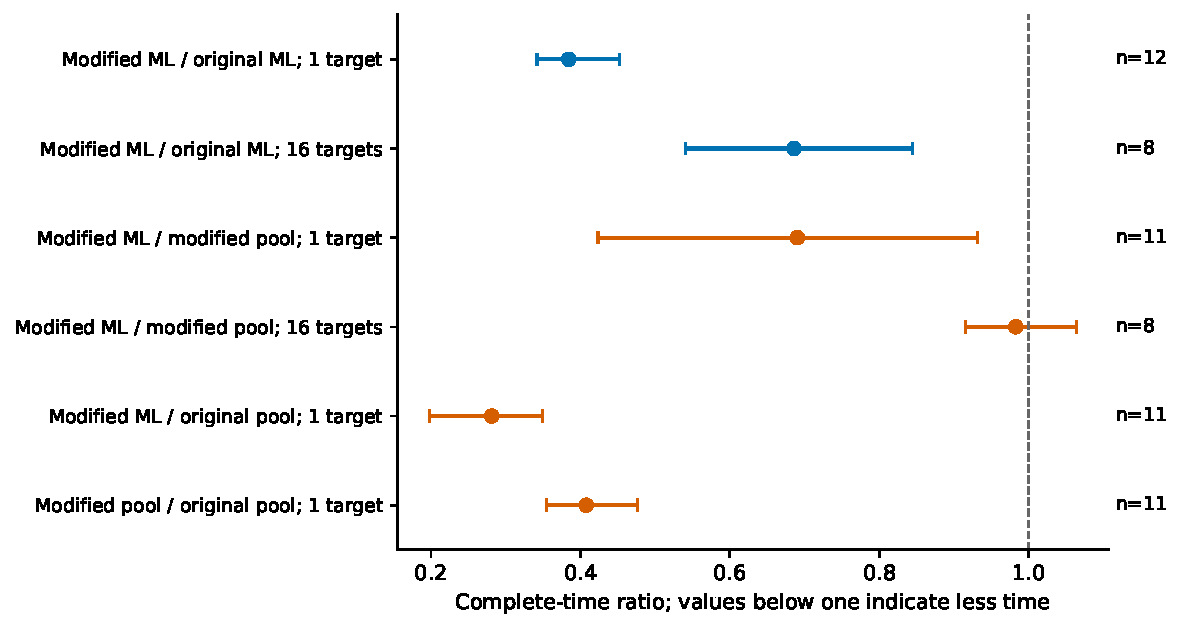
\includegraphics[width=\linewidth]{figures/responsive_exit_times.pdf}
\caption{Complete-time ratios for responsive Fermat shutdown and learned
seed selection. Points show geometric means of paired five-repeat
medians; intervals resample kinematic groups. Each row compares the
same physical targets, and values below one indicate less complete time. Here $n$ is the number of complete paired batches.}
\label{fig:responsive-exit-times}
\end{figure}
\FloatBarrier


\section{Complete native multiloop reductions}
\label{sec:complete-multiloop}
The preceding supplied-equation tests begin with an existing IBP pool.
To include the work needed to form that pool, we now give Kira physical
denominators and indexed target integrals and repeat equation generation
in every measured calculation. We also train a separate row model from
the algebraic work caused by choices inside Kira. This connects the
training objective to the intended reduction cost and permits a direct
comparison with Kira's own source-row choices.

\subsection{Physical families and independent targets}
The integral notation remains $I_{\boldsymbol a}$, with
$D_i=q_i^2-m_i^2+\mathrm{i}0$ as defined earlier. We use the following
ordered momentum lists:
\begin{align}
 \boldsymbol q_{\rm sunrise}
 &= (\ell_1,\ell_2,p-\ell_1-\ell_2,p-\ell_1,p-\ell_2),\\
 \boldsymbol q_{\rm box}
 &= (\ell_1,\ell_1-p_1,\ell_1-p_1-p_2,
     \ell_2,\ell_2-p_1-p_2,\ell_2-p_1-p_2-p_3,\nonumber\\
 &\hspace{2em}\ell_1-\ell_2,\ell_1-p_3,\ell_2-p_1),\\
 \boldsymbol q_{\rm vacuum}
 &= (\ell_1,\ell_2,\ell_3,\ell_1-\ell_2,
     \ell_2-\ell_3,\ell_1-\ell_3),\\
 \boldsymbol q_{\rm ladder}
 &= (\ell_1,\ell_1-p,\ell_2,\ell_2-p,\ell_3,\ell_3-p,
     \ell_1-\ell_2,\ell_2-\ell_3,\ell_1-\ell_3).
\end{align}
The first three sunrise entries, seven box entries and eight ladder
entries are physical propagators. Their remaining entries complete the
scalar-product basis and can appear with nonpositive indices. All six
vacuum entries are physical propagators. The first two lists contain
two loop momenta, and the last two contain three. In particular, the
three-loop vacuum and ladder systems couple the loop momenta through
shared propagators.

For each list, we expand the squared momenta in
$\ell_i\cdot\ell_j$ and $\ell_i\cdot p_j$ and check that the resulting
coefficient matrix has rank
\[
 N_{\rm sp}=\frac{L(L+1)}{2}+LE.
\]
Here $E$ is the number of independent external momenta, and $N_{\rm sp}$
is the number of independent scalar products involving loop momenta.
All fifteen family definitions pass this check, and their nonempty
external Gram matrices have nonzero determinants. This prevents a
dependent denominator list from entering the comparison.

All squared masses and external scalar products have fixed rational
values in a common squared-momentum unit, while the dimension $d$
remains symbolic. The reduction coefficients therefore belong to
$\mathbb Q(d)$. For the box, the external momenta satisfy
\[
 p_i^2=0,\qquad
 2p_1\cdot p_2=s,\qquad
 2p_1\cdot p_3=t,\qquad
 2p_2\cdot p_3=-s-t.
\]
The six training cases consist of two sunrise mass profiles
$(1,1,1)$ and $(1,2,3)$ with $p^2=-1,-2$ respectively, two massless
boxes with $(s,t)=(-1,-2),(-2,-3)$, and two vacuum profiles
$(1,1,1,1,1,1)$ and $(1,1,1,2,2,2)$. These profiles specify squared
masses in the displayed propagator order. Validation uses the sunrise
profile $(1,1,2)$ at $p^2=-3$, a box at $(s,t)=(-3,-4)$, and the vacuum
profile $(1,1,1,1,1,2)$.

The six reserved cases use boxes at $(s,t)=(-5,-7),(-7,-11)$,
vacuum profiles $(1,1,2,1,2,2)$ and $(1,2,2,1,2,2)$, and two ladder
instances. One ladder is massless with $p^2=-1$; the other has
$m_1^2=1$, all other squared masses zero, and $p^2=-2$. The ladder
topology appears only in the reserved set. The other reserved cases
test different kinematic or mass conditions within training topologies.
These tests concern rational kinematic points with symbolic $d$ and
do not establish performance for general symbolic multiscale
coefficients.

Targets are individual indexed integrals. We begin with the full-sector
corner, then increase each positive index by one and insert each
available auxiliary numerator once. We repeat this enumeration after
removing one, two and three physical denominators, retain at least two
physical denominators, and remove duplicate index vectors. The reserved
batches contain the first 32 or 128 targets in this fixed order. This
construction selects targets without using learned scores or reverse
construction paths.

\subsection{Seed regions, learned subsets and complete fallback}
For a batch $\mathcal T$, define
\[
 r_{\mathcal T}=\max_{\boldsymbol a\in\mathcal T}
                  \sum_i\max(a_i,0),\qquad
 s_{\mathcal T}=\max_{\boldsymbol a\in\mathcal T}
                  \sum_i\max(-a_i,0),\qquad
 b_{\mathcal T}=\max_{\boldsymbol a\in\mathcal T}
                  \sum_i\max(a_i-1,0).
\]
The last quantity is the largest total number of additional propagator
powers, also called dots. We specify Kira seed bounds
$(r_{\mathcal T}+\delta,s_{\mathcal T}+\delta,b_{\mathcal T}+\delta)$,
where $\delta=1$ defines the conservative reference region and
$\delta=0$ defines the smaller region. Kira still applies its native
symmetry, equation-generation and equation-selection procedures within
these bounds~\cite{Kira3}. The bounds are explicit input choices;
their difference is not a learned improvement to Kira.

The saved seed model scores the finite candidate region using the
ordered sum of the batch targets, with coefficient one for each target.
This sum supplies model context, while Kira still reduces every target
separately. Every sector corner, target and prescribed master that
belongs to the candidate region remains available. An additional
deterministic rule can retain all seeds with at most one dot or one
numerator power in total. The learned policy can add seeds above its
probability threshold, and a separate control applies the same
deterministic rule without model inference.

Kira first checks whether the selected system requires masters outside
the prescribed reference basis. A rejected subset triggers the
documented fallback sequence, and its time remains part of the
measurement. A final successful calculation must produce every
requested target and match its reference coefficient in $\mathbb Q(d)$.
Other failed attempts also move through the prescribed fallback sequence. A coefficient mismatch makes the complete workflow unsuccessful. Splitting a batch into groups of
32 targets bounds each calculation, but it also repeats equation
generation and process startup; the timing comparison includes both
effects.

\subsection{Training row choices on their algebraic consequences}
The new row model chooses a source among equations with the same
leading integral. It preserves Kira's native pivot and group order, and
Kira carries out every resulting row operation exactly. At state $S$,
the allowed action $q$ selects one such source row, which removes the
leading integral from the other rows in that group. The model therefore
acts on the changing native matrix through a restricted, explicitly
defined action set.

The first training objective measures the immediate symbolic insertion
time for each source. We clone the destination rows, apply the exact
native update, and average two rotated measurement orders while
excluding clone time. This measures local arithmetic cost, but it does
not include the equations created by later eliminations. We therefore
also measure a continuation cost,
\begin{equation}
 C(S,q)=\sum_{j\in\mathcal U(S,q)}(1+2n_j).
 \label{eq:continuation-cost}
\end{equation}
Here $\mathcal U(S,q)$ is the sequence of committed forward insertions
after choosing $q$ and then following Kira's native choices, and $n_j$
is the number of nonzero coefficients in the source of insertion $j$.
The count assigns one division and two coefficient operations per
source entry. It is an algebraic operation estimate tied to measured
native insertions; it does not count Fermat's internal polynomial
operations or back substitution.

We choose up to four evenly spaced eligible states from the saved
local-cost sample in each development case, which contains at most
100 measured groups. We prefer groups with at least three source
choices and use smaller groups when no such group is available. Each alternative receives a separate complete Kira continuation.
The recorded pivot and all candidate features must match the original
state, and the final master coefficients must match the reference
reduction before its cost can enter training. The resulting labels
measure a choice followed by native continuation. They do not prove a
globally minimum reduction path.

Each candidate has eighteen features describing row length, coefficient
text length and operations, overlap with destination columns, estimated
new entries, and its position relative to Kira's preferred source.
A linear fit to log continuation cost retained the native source in all
nine validation states. We therefore also fit a small regression tree~\cite{CART1984},
which can represent conditions involving several features.

For this tree, the target is the normalized change in measured
continuation cost,
\[
 y_q=\frac{C(S,q)-C(S,0)}
           {\max\{1,\max_{q'}C(S,q')-\min_{q'}C(S,q')\}},
 \qquad
 \widehat y_q=h(\boldsymbol x_q-\boldsymbol x_0).
\]
The index $0$ denotes Kira's preferred source, $\boldsymbol x_q$ is the
candidate feature vector, and $h$ is the fitted tree. Lower targets
correspond to fewer recorded operations. We fix $\widehat y_0=0$ and
fit the remaining candidates with a weighted least-squares loss that
gives each training family equal weight. Validation selects tree
depth, minimum leaf population, target normalization and the required
predicted gain.

The selected tree has 21 nodes, depth four and at least two training
examples in each leaf. Its training set contains 68 candidate
continuations in 24 states from six families, while validation contains
30 candidates in nine states from three families. All 98 continuations
match their exact reference reductions. The tree changes nine training
choices and three validation choices, with family-weighted continuation
count ratios of 0.998602 and 0.999967 to the native choices. These
ratios measure individual choices followed by native continuation;
the next test must determine the effect of using the model repeatedly.

The model chooses the lowest predicted score and reports
\[
 P(q\mid S)=\frac{\exp(-\widehat y_q)}
                 {\sum_{q'}\exp(-\widehat y_{q'})}.
\]
This quantity expresses a relative model score, with no calibration
claim. Kira evaluates each score directly in compiled code. Groups with two rows or more than
32 rows keep the native source, which also avoids feature construction
for those groups. We preserve the original neural checkpoint and both
earlier linear fits as separate artifacts, and hold the final tree
fixed during reserved testing.

The seed implementation also reads its unchanged weight archive once
per process and retains at most two sets of family and candidate
embeddings within a workflow. A new target batch still receives its
own target features and scores. Independent checks compare every
probability with the original implementation and compare native tree
scores and choices with the Python model. These changes reduce
repeated loading and feature preparation while preserving the tested
seed predictions.

\subsection{Complete timing and reference checks}
Every final trial starts a new process and includes input preparation,
model loading and inference, native IBP generation and selection,
symbolic elimination, back substitution, exact coefficient comparison,
and all failed attempts and fallback reductions. Evidence compression
follows the stop time. These checks establish reduction to the prescribed reference basis;
they do not prove global minimality of the master set.
We report the initial reference calculation separately as common
benchmark preparation. Each policy receives the same prescribed
master basis and exact comparison result within a case.

All controls use the responsive Fermat shutdown from the preceding
section. We compare both the unchanged reduction executable with that
shutdown fix and an instrumented executable that keeps native row
choices. This separates the cost of measurement and integration from
the learned action. We also compare smaller deterministic regions and
matched deterministic seed subsets, since either could explain a gain
over conservative bounds.

Each trial uses one calculation thread, a bounded scratch directory
and limits on elapsed time and process-tree memory. Production trials
have 128 MiB of scratch space, a 2,400 MiB solver address-space limit, and a 2,100 MiB solver process-tree resident-memory limit. The enclosing worker has a 2,800 MiB address-space limit and a 2,600 MiB process-tree resident-memory limit. A single common-reference calculation
can use 256 MiB while retaining the same symbolic bounds, and the
storage ledger includes additional monitoring headroom. Final comparisons
use paired cases and report completion counts alongside time ratios.
Repeated runs reduce timing noise within a case, while different
kinematic instances remain distinct from different topologies.
The reserved results do not select the policy or its thresholds.

\subsection{Reserved results and complete-calculation cost}
The frozen comparison contains six reserved cases, two target-batch
sizes, nine policies and three repetitions of each policy. Each trial
begins with physical denominators and includes native IBP equation
generation. The results and exact evidence are available with the
comparison data~\cite{KiraCompleteMultiloopData}.

We measured 324 of 324 planned trials, and 324 completed every target with exact reference coefficients. The records retain 0 unsuccessful measured trials and 0 skipped trials. The independent audit checked 550 successful native reductions, including the training continuations and reserved attempts, and made 114,965 coefficient comparisons by exact polynomial cross multiplication. All 98 recorded training and validation continuations passed. The separate larger-region check completed 6 of 6 cases. These comparisons verify reduction to the prescribed basis; a finite region check does not prove that the basis is globally minimal.

The measured workflows contain 585 native reduction attempts. Kira rejected 66 attempted subsets because they required masters outside the prescribed basis. The remaining unsuccessful attempts comprise 84 other Kira errors, 3 elapsed-time limits. These attempts remain in complete-workflow times, and the fallback sequence determines whether every target can still be reduced within the budget.

The common reference preparation completed 12 of 12 case--batch calculations. The successful reference times ranged from 5.967 to 28.083 seconds and are outside the paired production timings. The two 128-target box cases use 8 master integrals each. Both contain 8 zero targets and 3 targets already in the master basis, leaving 117 nonzero targets that require reduction in each case. The two 128-target vacuum cases use 11 and 17 master integrals, respectively. The first contains 4 zero targets and 8 targets already in the master basis, leaving 116 nonzero targets that require reduction. The second contains 4 zero targets and 13 targets already in the master basis, leaving 111 nonzero targets that require reduction. The two 128-target ladder cases use 5 and 21 master integrals, respectively. The first contains 14 zero targets and 0 targets already in the master basis, leaving 114 nonzero targets that require reduction. The second contains 14 zero targets and 1 targets already in the master basis, leaving 113 nonzero targets that require reduction. 

The following ratios use only case--batch pairs for which both policies completed all three repetitions. We take the median within each case and batch, average log ratios within a case, and then give cases equal weight. Ratios of operation counts also require positive counts in both methods. The intervals use 5,000 resamples of the fixed physical cases, so they describe this sample rather than a general distribution of multiloop families.

\subsubsection{Seed selection and deterministic controls}
Validation selected the smaller-region learned seed policy at probability threshold $0.01$. Its complete-time ratio to instrumented native Kira was 1.118 on the validation sample; this selection therefore did not establish an aggregate validation gain. On reserved tests, its ratio to the responsive stock control is 0.742 with descriptive interval $[0.560,1.009]$, and its ratio to the instrumented native control is 0.755 with descriptive interval $[0.573,1.050]$. Against the smaller deterministic region with fallback, the ratio is 0.916 with descriptive interval $[0.723,1.152]$. Against the same low-complexity coverage rule without ML, the ratio is 0.833 with descriptive interval $[0.679,1.010]$. These controls separate the effects of region size, deterministic coverage, model inference and the learned additions.

For 32 targets, the learned seed ratio to responsive stock Kira is 0.713 with descriptive interval $[0.543,0.967]$, using 6 complete paired batches. The corresponding geometric mean median times are 10.490 and 14.720 seconds. For 128 targets, the learned seed ratio to responsive stock Kira is 0.772 with descriptive interval $[0.558,1.082]$, using 6 complete paired batches. The corresponding geometric mean median times are 13.723 and 17.764 seconds. 

For the two-loop boxes, the seed-to-stock time ratio is 0.563 with descriptive interval $[0.531,0.598]$. Its ratio to the smaller deterministic region is 0.642 with descriptive interval $[0.627,0.658]$. Its ratio to the matched coverage rule is 0.606 with descriptive interval $[0.567,0.648]$. For the three-loop vacuum integrals, the seed-to-stock time ratio is 1.266 with descriptive interval $[1.180,1.357]$. Its ratio to the smaller deterministic region is 1.291 with descriptive interval $[1.245,1.338]$. Its ratio to the matched coverage rule is 1.093 with descriptive interval $[1.016,1.175]$. For the three-loop ladders, the seed-to-stock time ratio is 0.573 with descriptive interval $[0.554,0.592]$. Its ratio to the smaller deterministic region is 0.928 with descriptive interval $[0.852,1.010]$. Its ratio to the matched coverage rule is 0.871 with descriptive interval $[0.833,0.910]$. These topology breakdowns retain every case in the stated class. The ladder class tests a topology absent from the new row-training and validation data.

The learned seed ratio for the initially generated equations summed across attempts is 0.086 with descriptive interval $[0.049,0.152]$ relative to native Kira. The learned seed ratio for the committed forward coefficient-operation estimate is 0.798 with descriptive interval $[0.655,0.992]$ relative to native Kira. The first generation count in each native attempt defines the equation measure; later selection counts are not added to it. The operation estimate follows Eq.~\eqref{eq:continuation-cost}, and all attempted stages contribute when a workflow requires fallback.

\begin{figure}[htbp]
\centering
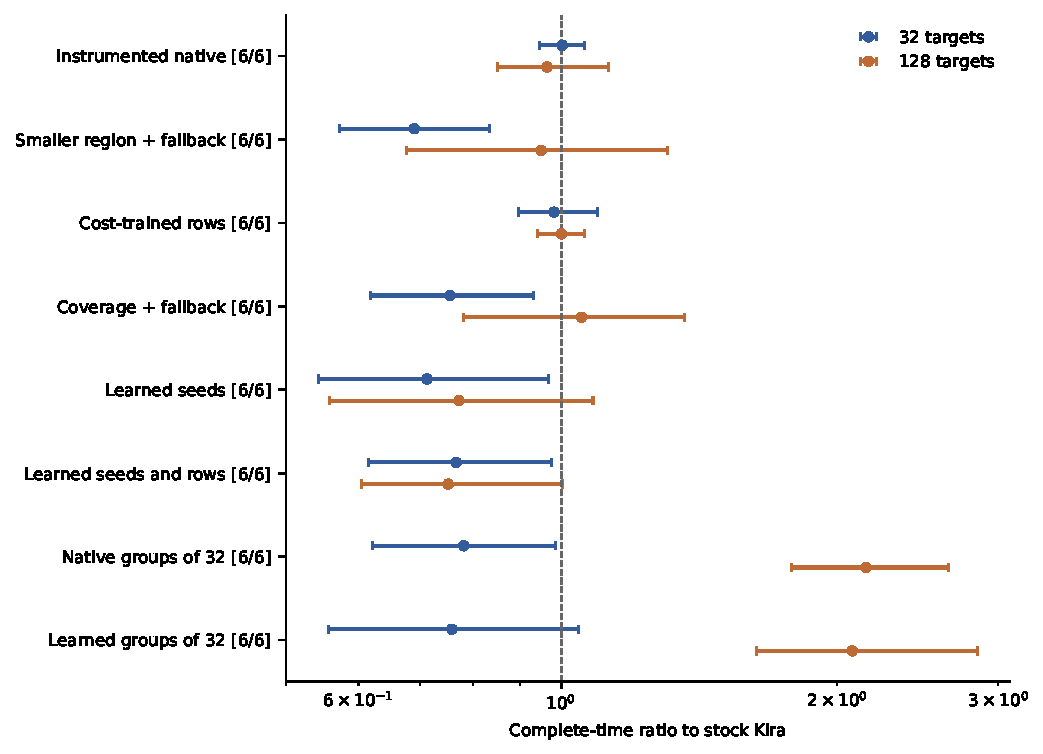
\includegraphics[width=\linewidth]{figures/native_multiloop_times.pdf}
\caption{Complete-time ratios to responsive stock Kira for 32 and 128 indexed targets. Points use medians of three exact repetitions and equal case weights. Bars show descriptive case-resampling intervals; the labels give complete paired batch counts. A ratio below one means lower measured time in the stated paired cohort.}
\label{fig:native-multiloop-times}
\end{figure}
\subsubsection{Repeated row decisions in the changing matrix}
The cost-trained row tree has a complete-time ratio of 1.008 with descriptive interval $[0.937,1.078]$ to the instrumented native policy. Its forward coefficient-operation ratio is 1.003 with descriptive interval $[0.983,1.021]$, while the measured forward-stage time ratio is 0.943 with descriptive interval $[0.828,1.033]$. The paired geometric mean forward times are 0.091 seconds for native choices and 0.085 seconds for the tree, while their complete times are 15.887 and 16.013 seconds. Most measured time therefore lies outside this recorded forward stage. The sampled continuation objective measures one altered source choice followed by native choices. Repeated tree choices change the later matrices and can therefore change the cost in a different direction. The full-workflow results determine whether the trained model saves work in this use.

The combined seed and row policy has a complete-time ratio of 0.759 with descriptive interval $[0.613,0.962]$ to responsive stock Kira. Its paired geometric mean median time is 12.280 seconds, compared with 11.998 seconds for seeds alone. The row addition therefore does not lower this point estimate. Combining two decisions requires a separate measurement because a different seed set changes the equations on which the row policy acts.

\begin{figure}[htbp]
\centering
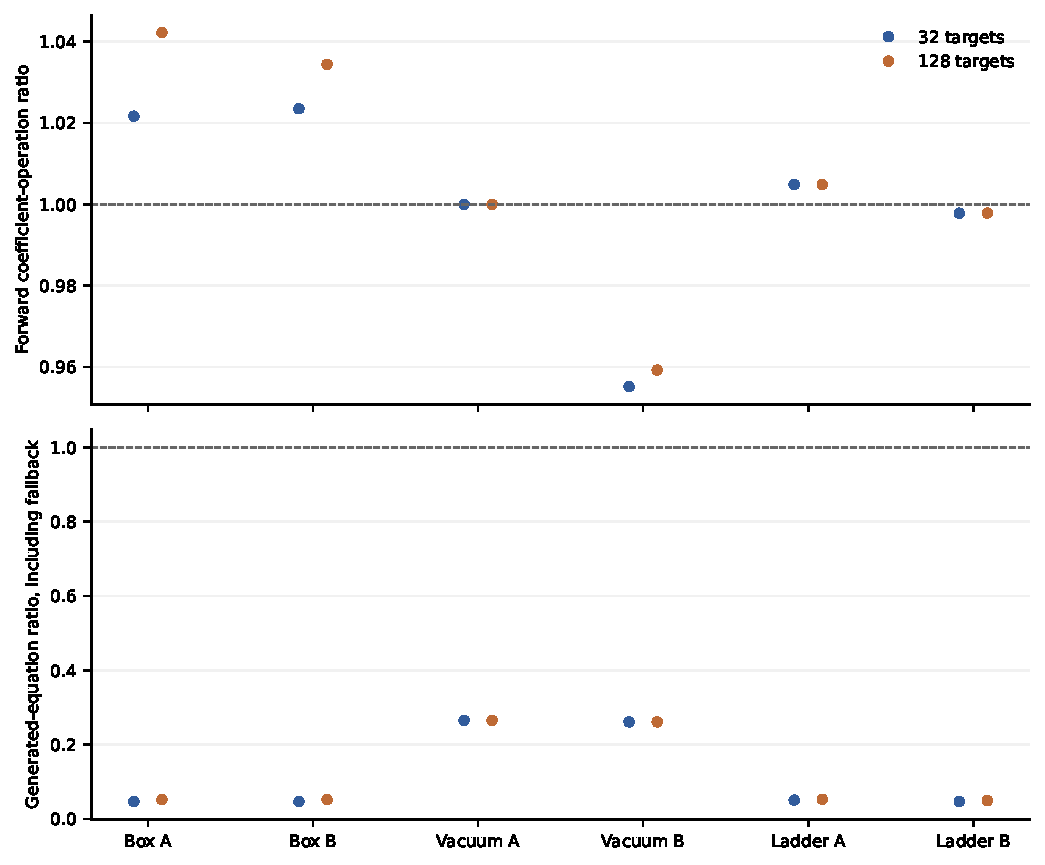
\includegraphics[width=\linewidth]{figures/native_multiloop_operations.pdf}
\caption{Per-case median work ratios in the reserved comparison. The row panel measures committed forward coefficient operations relative to the same instrumented native policy. The seed panel measures initial generated equations, summed over attempts, relative to native Kira. Cases A and B follow the parameter order given in the text. Counts concern different stages and do not measure Fermat's internal polynomial work.}
\label{fig:native-multiloop-operations}
\end{figure}
\subsubsection{Completion of larger target batches}
With 32 targets, responsive stock Kira completed 18 of 18 trials. For the learned seed workflow, 18 of 18 completed, including 6 rescued by fallback. For the combined workflow, 18 of 18 completed, including 6 rescued by fallback. For native groups of 32 targets, 18 of 18 completed, including 0 rescued by fallback. For combined groups of 32 targets, 18 of 18 completed, including 6 rescued by fallback. 

With 128 targets, responsive stock Kira completed 18 of 18 trials. For the learned seed workflow, 18 of 18 completed, including 6 rescued by fallback. For the combined workflow, 18 of 18 completed, including 6 rescued by fallback. For native groups of 32 targets, 18 of 18 completed, including 18 rescued by fallback. For combined groups of 32 targets, 18 of 18 completed, including 18 rescued by fallback. 

For 128 targets, splitting the native workflow gives a time ratio of 2.151 with descriptive interval $[1.783,2.647]$ to stock Kira. Splitting the combined workflow gives 2.078 with descriptive interval $[1.631,2.845]$. The separate fallback counts show whether completion improves; the paired times include repeated generation and process startup.

\begin{figure}[htbp]
\centering
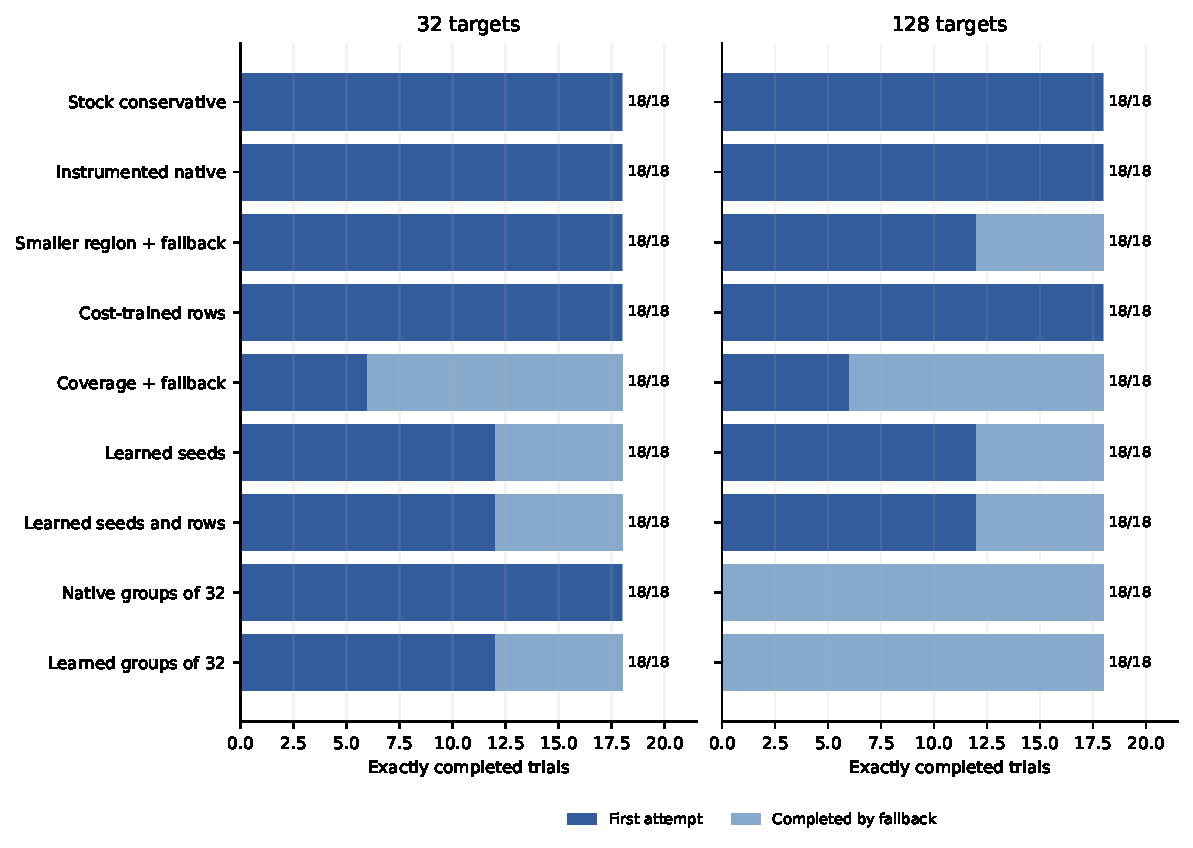
\includegraphics[width=\linewidth]{figures/native_multiloop_completion.pdf}
\caption{Completion of all requested targets under the fixed time and storage limits. The filled components distinguish successful initial reductions from reductions completed through fallback. Unfilled trials include failed or explicitly skipped outcomes. Each policy has eighteen planned trials at each batch size.}
\label{fig:native-multiloop-completion}
\end{figure}
\subsubsection{Scope and resource outcomes}
The largest recorded production process-tree memory use was 106.8 MiB, and the largest monitored production scratch allocation was 1.0 MiB. Among unsuccessful attempts, 7 logs report an allocation failure and 10 report recursive termination; these diagnostic counts can overlap. The fixed process limits constrain these outcomes, and the logs alone do not establish exhaustion of physical RAM. The workflow retains their costs and follows the same fallback rule. A separate post-comparison check repeated the smaller seed region for the 128-target validation box using both the responsive stock executable and the instrumented native executable. Both reported \texttt{std::bad\_alloc} under the same solver limits, so this failure also occurs without the row-policy hook. This check concerns the failure mechanism and supplies no additional timing comparison; it leaves all frozen reserved settings unchanged.

One scheduler interruption stopped a test worker when the sum of its processes' virtual address spaces exceeded the job limit. We preserved its completed records and resumed only missing work with a larger scheduler address-space allowance, while keeping the measured physical-memory, scratch and elapsed-time limits fixed. This interruption is recorded separately from completed workflow timings. With the resumed case excluded, the learned seed to stock complete-time ratio is 0.676 with descriptive interval $[0.549,0.963]$. With the resumed case excluded, the learned row to native complete-time ratio is 1.039 with descriptive interval $[0.991,1.102]$. The tests include two- and three-loop systems at fixed rational kinematics, a finite prescribed seed region and a restricted source-row action. They do not establish a speedup for arbitrary symbolic kinematics, every multiloop topology, or the earlier restricted collection through twelve loops.
\FloatBarrier


\section{Integrated seed and row policies with bounded execution}
\label{sec:integrated-runtime}
The complete reductions in Section~\ref{sec:complete-multiloop} show that a learned
choice can save algebraic work while other parts of the calculation determine
most of the elapsed time. We therefore examine both the cost of applying the
models and the native operations that surround them. Every comparison in this
section starts from physical denominators, generates IBP equations and checks
the final master coefficients. We retain the earlier checkpoints and results,
and use separate training, validation and reserved cases for the new policies.

\subsection{Removing costs shared by both decision methods}
Back substitution replaces the remaining nonmaster integrals in each triangular
equation with their reductions. If the equation for $I_{\boldsymbol a}$ contains
$I_{\boldsymbol b}$ on its right-hand side, the latter reduction must be available
before the former equation can finish. We represent this dependency by the
directed edge
\[
 I_{\boldsymbol b}\longrightarrow I_{\boldsymbol a}.
\]
A topological order is a sequence in which every dependency appears before the
equation that uses it. The modified single-worker schedule constructs this order
from the loaded equations, preserves the native arithmetic and rejects a cycle
or an invalid dependency. This permits one bounded group of back-substitution
workers. The inspected native implementation created helper workers for each
sector range, even when the calculation used one arithmetic worker.

An initial merge that retained the loaded row order reached a dependency wait
and exceeded its time limit. The corrected order completed all six subsequent
bounded pilot reductions and reproduced their reference coefficients. The
corresponding smaller-region native control reported an allocation failure.
These are development checks of the scheduling change. They do not attribute a
gain to either learned model or establish a general memory-exhaustion mechanism.

The calculation also creates temporary databases. We compare the same native
reductions with those databases on project storage and on the compute node's
temporary storage. The eight exact pilot runs use the same resource limits and
two repetitions of each region and storage condition. Their geometric mean time
ratio for node storage relative to project storage is $0.307$. We use node
storage for all later learned and deterministic controls. Both controls therefore
receive the same scheduling and storage improvements.

\subsection{Applying the seed model with unchanged probabilities}
The seed policy retains the trained neural weights and the finite candidate
region described earlier. For each batch, it constructs the family features,
the ordered target features and the candidate index features before predicting
a separate probability for every seed. We construct the index features in
arrays and reuse shared family information so that the model performs less
repeated preparation.

A parity check compares 5,000 generated index vectors and all candidate
predictions for the nine development profiles. The feature values, embeddings
and final probabilities agree exactly with the preceding implementation. In
the development box checks with 3,510 candidates, shared feature construction
and prediction decrease from approximately $0.08$ to $0.01$ seconds. These
component measurements motivate the implementation change; complete-workflow
comparisons must also include model loading, equation generation, exact algebra
and any fallback.

The selected seeds always retain the prescribed mandatory integrals and the
stated deterministic coverage rule. Kira checks whether the resulting system
introduces masters outside the reference basis. An insufficient set triggers
the fixed fallback sequence, and the elapsed time includes the unsuccessful
attempt. Final coefficients must agree with the common reference in
$\mathbb Q(d)$.

\subsection{Estimating cancellations before a row choice}
The row model chooses among source equations with the same leading integral,
as in the preceding native experiment. To include cancellations in its
description of each choice, consider source row $\boldsymbol u_q$ and
destination row $\boldsymbol v_j$, with common leading column $p$ and nonzero
source coefficient $u_{qp}$. Exact elimination forms
\[
 v'_{jk}=v_{jk}-\frac{v_{jp}}{u_{qp}}u_{qk}.
\]
A resulting coefficient vanishes when
\[
 v_{jk}u_{qp}-v_{jp}u_{qk}=0.
\]
We estimate this condition by evaluating the rational coefficients at
$d=17$ and $d=19$ modulo the prime $2\,147\,483\,647$. Two zero evaluations
supply a feature estimate of cancellation; they do not certify a symbolic
identity. Kira still performs the exact update, and the final reduction still
undergoes an exact coefficient check. Unsupported expressions and poles cause
the policy to retain the native source.

Let $\widehat n_{jq}$ be the estimated number of surviving entries in
destination $j$ after using source $q$. Six additional features describe the
total $\sum_{j\ne q}\widehat n_{jq}$, the cancellation fraction, the largest
resulting row, the number of zero rows, the sum
$\sum_{j\ne q}\widehat n_{jq}^{\,2}$, and whether the modular estimate is valid.
They extend the previous eighteen features to twenty-four. The implementation
bounds the group size, coefficient text and modular cache, and retains native
behavior outside these limits.

Independent checks compare the evaluator with exact rational arithmetic for
210 expressions and three row-choice fixtures. A separate in-process comparison
checks shared feature construction against the original formula in 4,041
changing row groups. Python and the compiled policy also agree on all 3,247
recorded decisions in that check, and all three full reductions match their
reference coefficients. Shared construction calculates each row's length and
coefficient statistics once per group and each pairwise overlap once.

\subsection{Learning from local cost and complete trajectories}
Each of the six training profiles and three validation profiles has an ordinary
batch and a deeper batch. The deeper batch includes integrals with two extra
propagator powers and mixed numerator and propagator powers. Both batches from
a physical profile remain in the same partition. Collection gives 2,520
eligible training groups and 1,372 validation groups, with exact reference
agreement required before any group can enter training.

We first fit small regression trees to immediate insertion time, resulting
coefficient text length, and a combination of these quantities. The
time-selected trees keep every native choice in their recorded validation
groups. The coefficient-length tree changes 371 choices and gives a
family-weighted immediate coefficient-length ratio of $0.920$, accompanied by
an insertion-time ratio of $1.097$. These labels describe a single group.
Repeated deployment can change later matrices, so the full reduction supplies
the required cost comparison.

The next search therefore evaluates a policy throughout the native forward
reduction. A candidate assigns source $q$ the score
\[
 s_{\boldsymbol w}(S,q)=\boldsymbol w^{\mathsf T}\boldsymbol x(S,q),
 \qquad
 q^*(S)=\underset{q}{\operatorname{arg\,min}}\,
             s_{\boldsymbol w}(S,q),
\]
where $S$ is the current row group, $\boldsymbol x(S,q)$ is its feature vector
and $\boldsymbol w$ is the policy's coefficient vector. Ties retain the native
source. The bounded candidate set varies the emphasis on source length,
coefficient length, predicted surviving entries, squared resulting row lengths
and preference for the native source.

We evaluate eighteen coefficient vectors on all twelve training batches.
For each complete trajectory, the forward-work estimate remains
$\sum_j(1+2n_j)$ from Eq.~\eqref{eq:continuation-cost}. This count now includes
every committed update caused by repeated policy choices. We rank candidates
by the geometric mean ratio to native work, first averaging the ordinary and
deeper batches within each physical profile and then giving profiles equal
weight. Thus later algebraic consequences enter the training objective directly.
The measured count excludes Fermat's internal polynomial operations and
back substitution, which remain covered by the complete-time measurement.


The two nontrivial linear policies retained for the final comparison use
\begin{align}
 s_A(S,q)&=
 2\log(1+n_q)+
 \log\!\left(1+\sum_{j\ne q}\widehat n_{jq}\right),\\
 s_B(S,q)&=
 \tfrac12\log(1+n_q)+
 \log\!\left(1+\sum_{j\ne q}\widehat n_{jq}\right)
 +0.3\log\!\left(1+\sum_{j\ne q}\widehat n_{jq}^{\,2}\right)
 -0.01\,\delta_{q0}.
\end{align}
Here $n_q$ is the number of entries in source row $q$, and
$\delta_{q0}$ is one for the native source and zero for another source.
The lower score selects the source. These coefficient vectors come from
the stated finite search; validation then selects which vector to use for
each topology. The small native-source preference in $s_B$ reduces changes
when its other features give nearly equal scores.

Separate validation compares the selected policies with native choices and
a deterministic rule that minimizes the predicted number of surviving entries.
It also measures the seed policy alone and the combined seed and row policy.
A model reports the normalized score
\[
 P(q\mid S)=
 \frac{\exp[-s_{\boldsymbol w}(S,q)]}
 {\sum_{q'}\exp[-s_{\boldsymbol w}(S,q')]}.
\]
This gives a relative preference among the supplied actions, with no
calibration or global-optimality claim. Reserved cases do not select weights,
thresholds or deployment rules.

\subsection{Timing a complete integrated workflow}
All methods use fresh processes, the same temporary storage and the same
bounded back-substitution schedule. Production timing includes preparation,
prediction, equation generation and selection, elimination, back substitution,
exact comparison and every required fallback. A child-exit notification ends
the wait promptly and avoids adding the monitor's polling interval to short
calculations. Detailed training traces remain disabled during production
timing, while aggregate operation and time counters remain enabled.

The reference reduction and prescribed master basis are common benchmark
preparation and remain outside the paired production time. Successful trials
must reduce every supplied target to that basis with exact coefficients.
At most two production reductions run concurrently, each with 128 MiB of
temporary storage and the preceding process-memory limits. The project ledger
reserves storage for temporary files, retained records, publication copies and
the local report while remaining below the user's combined 10 GB ceiling.

\subsection{Reducing the cost of a single model call}
The vector implementation accelerates repeated inference, but a short
reduction also pays for loading its numerical library. We therefore export
the same trained weights to a compiled evaluator that reads the same family,
target and candidate features. The evaluator uses single-precision arithmetic
and preserves the network's matrix operations, nonlinear functions and
attention calculation. Different accumulation orders can change the last
digits of a probability, so we check both probabilities and the selected sets.

Across thirty-six development contexts, the largest absolute probability
difference is $9.48\times10^{-6}$. All selection masks agree at thresholds
$0.003$, $0.01$, $0.03$, $0.1$, $0.3$ and $0.5$. A further forty-eight fresh-process
checks use eight validation contexts, two implementations and three repetitions.
Their selected sets also agree. The compiled implementation takes between
$0.264$ and $0.804$ times the numerical-library implementation's median
preparation and inference time across these contexts. Its arithmetic alone
is slower in the warm tests; the fresh-process benefit comes from the lower
startup cost. Production comparisons therefore retain startup in the timed
workflow.

We also reduce the row policy's feature cost. Once training selects a sparse
coefficient vector $\boldsymbol w$, only features with $w_k\ne0$ affect its score.
The production evaluator computes those features, while the diagnostic path
retains the full vector. Thirty-six complete comparisons check three policies
on six validation batches with this optimization enabled and disabled.
The selected sources, committed operations and exact exports agree. The
deterministic cancellation rule receives the same feature optimization, and
its coverage control loads no neural model. These controls prevent model
startup and unused feature work from creating an artificial learned advantage.

\subsection{Selecting thresholds from complete reduction cost}
The seed probabilities describe membership in the recorded construction data.
Their classification threshold need not minimize the cost of a new native
reduction. We therefore select an execution threshold using only the twelve
native training batches. For each threshold $\tau$ in the six-value set above,
the policy selects every candidate whose probability is at least $\tau$,
together with the mandatory coverage seeds. The search retains all time spent
on unsuccessful attempts and the fixed native fallback.

Let $T_{i,\tau}$ be this complete time for training batch $i$, and let
$T_{i,\mathrm{native}}$ be the time for the smaller native region with its
fallback. Batches share a threshold when they have the same topology, largest
number of additional propagator powers and largest total numerator power.
For each such class $\mathcal C$, training selects
\[
 \tau_{\mathcal C}=
 \underset{\tau}{\operatorname{arg\,min}}\,
 \exp\left[
  \frac{1}{|\mathcal C|}
  \sum_{i\in\mathcal C}
  \log\frac{T_{i,\tau}}{T_{i,\mathrm{native}}}
 \right].
\]
Here $|\mathcal C|$ is the number of training batches in that class.
The scan contains ninety-six complete workflows, including the smaller
native and deterministic coverage controls. This threshold search changes
execution settings and preserves the earlier classification tests at their
original threshold.

One development subset exposed an additional admission requirement. Its
export still contained an integral outside the prescribed master basis,
although the native master check had accepted the initial system. The exact
reference comparison rejected the result. We now also inspect every
integral on the right-hand side of the exported reduction. An extra integral
marks an incomplete reduction and triggers the fixed expansion of the seed
region. A disagreement between coefficients in the admitted basis stops the
calculation. The original rejected result remains in the evidence, and its
replacement workflow includes the unsuccessful subset's elapsed time.

\subsection{Controls and the scope of the optimization}
The smaller native control starts with the target's own bounds on propagator
and numerator powers and expands them if needed. The conservative control
starts one step beyond these bounds. The learned and deterministic coverage
methods first try a subset of the smaller region, then the whole smaller
region, then the conservative region. Row policies make each source choice
inside the current native matrix throughout these attempts. This comparison
separates the effect of a learned subset from the effect of starting with
fewer native equations.

An additional experiment changes the database settings only for fresh,
disposable trial directories. Three paired exact reductions give a median
time ratio of approximately $1.011$ to the unchanged settings, so the final
configuration retains the usual database settings. A separate system-call
diagnostic finds negligible time in database flushes for the examined box
calculation. Disabling synchronization or moving a journal to memory changes
recovery guarantees~\cite{SQLitePragmas}; the retained configuration receives
no performance claim from this rejected experiment.

These searches compare a finite set of models and execution choices under
the stated memory and storage limits. They identify configurations with lower
measured cost on their supported inputs. They do not prove a globally minimal
number of algebraic operations or a globally shortest calculation time.

\subsection{Initial independent tests of the integrated calculation}
The initial comparison uses eight physical profiles that did not select the
weights, thresholds or execution rules. Two two-loop sunrise profiles have
squared masses $(1,2,2)$ and $(1,2,4)$, with external invariant $p^2=-5$ and
$p^2=-7$, respectively. Two massless double-box profiles have
$(s,t)=(-11,-13)$ and $(-13,-17)$. The three-loop vacuum profiles have squared
masses $(1,1,1,1,1,3)$ and $(1,1,1,3,3,3)$. The three-loop ladder profiles have
one squared mass equal to one, all other physical propagator masses equal
to zero, and $p^2=-3$ or $-5$. All values use the common arbitrary mass unit
and denominator conventions of Section~\ref{sec:complete-multiloop}.
The dimension $d$ remains symbolic. The ladder topology remains absent
from the new row-policy training and validation data.

Each sunrise profile supplies its ordinary twenty-one-target batch and
a deeper thirty-two-target batch. Each other profile supplies batches of
thirty-two and 128 targets. We compare seven methods on these sixteen
batches: the conservative native region, the smaller native region,
the deterministic cancellation rule, deterministic seed coverage, the
seed model, the row model and both models together.
Five repetitions per method give 560 planned workflows. We rotate and
reverse method order within each physical profile. All methods use the
same prescribed master basis, exact coefficient checks, temporary storage
and single-worker schedule~\cite{KiraIntegratedRuntimeData}.

The validation-selected row score emphasizes source length for the boxes
and uses the mixed score for the sunrise and vacuum cases. The transfer
test also uses the mixed score for the ladder topology. Seed thresholds
come from the training classes; an unseen class uses the predefined
threshold $0.01$. The complete comparison executes the model ablations
even where validation recommends native execution, so an unfavorable model
cost remains visible in the results.

The recorded time begins with per-workflow preparation and ends after
the final exact check and cleanup. It includes model import, weight loading,
feature construction, prediction, every native generation and elimination
attempt, and every fallback. Python interpreter launch, the common reference
calculation, shared integrity checks and result compression remain outside
this interval. Every candidate model and control uses the same timing
boundary.

For each batch and method, we take the median of five repetitions.
We then form paired ratios, average their logarithms within each physical
profile and give the eight profiles equal weight. The descriptive intervals
resample whole physical profiles while retaining their two batches.
A topology-specific interval therefore contains only two independent profiles.
Repeated timings measure execution variation; they do not create additional
independent integral families.

The comparison records 560 workflows, of which 560 complete every target with the prescribed coefficients. It retains all 670 native attempts, including unsuccessful seed subsets. The independent audit reparses native exports and checks rational coefficients by exact polynomial cross multiplication in $\mathbb Q(d)$. Across the full development and test record, it reparses 2,386 successful native reductions and checks 507,630 coefficient comparisons. The separately retained development basis rejection remains a failed attempt and supplies no accepted reduction.

\subsection{Measured model effects against matched native choices}
Figure~\ref{fig:integrated-runtime-times} compares each model with the smaller
native control. This control receives the same runtime improvements and
starts from the same target bounds. The comparison therefore tests whether
the learned decisions save enough work to cover their own cost.

The seed policy has a complete-time ratio of 1.149, with descriptive interval $[1.021,1.311]$, relative to the smaller native control. Its point estimate corresponds to a 14.9\% increase in the profile-weighted complete time.

The row policy has a complete-time ratio of 1.004, with descriptive interval $[0.991,1.016]$, relative to the smaller native control. Its point estimate corresponds to a 0.4\% increase in the profile-weighted complete time.

The combined policy has a complete-time ratio of 1.165, with descriptive interval $[1.036,1.323]$, relative to the smaller native control. Its point estimate corresponds to a 16.5\% increase in the profile-weighted complete time.

These aggregate values combine inputs with different equation-generation and
elimination costs. The separate physical classes show where a model contributes
a measured saving and where its additional attempt or decision cost dominates.

For the two-loop sunrise profiles, the seed, row and combined complete-time ratios are 1.388, 0.990 and 1.424, respectively. Their descriptive intervals are $[1.386,1.390]$, $[0.975,1.005]$ and $[1.384,1.464]$. These values average the two tested batches within each of the two physical profiles.

For the two-loop double-box profiles, the seed, row and combined complete-time ratios are 0.953, 1.003 and 0.961, respectively. Their descriptive intervals are $[0.945,0.960]$, $[0.983,1.024]$ and $[0.953,0.968]$. These values average the two tested batches within each of the two physical profiles.

For the three-loop vacuum profiles, the seed, row and combined complete-time ratios are 1.309, 1.010 and 1.287, respectively. Their descriptive intervals are $[1.110,1.543]$, $[0.997,1.022]$ and $[1.104,1.500]$. These values average the two tested batches within each of the two physical profiles.

For the three-loop ladder profiles, the seed, row and combined complete-time ratios are 1.007, 1.013 and 1.047, respectively. Their descriptive intervals are $[1.003,1.011]$, $[1.003,1.023]$ and $[1.002,1.094]$. These values average the two tested batches within each of the two physical profiles.

\begin{figure}[htbp]
\centering
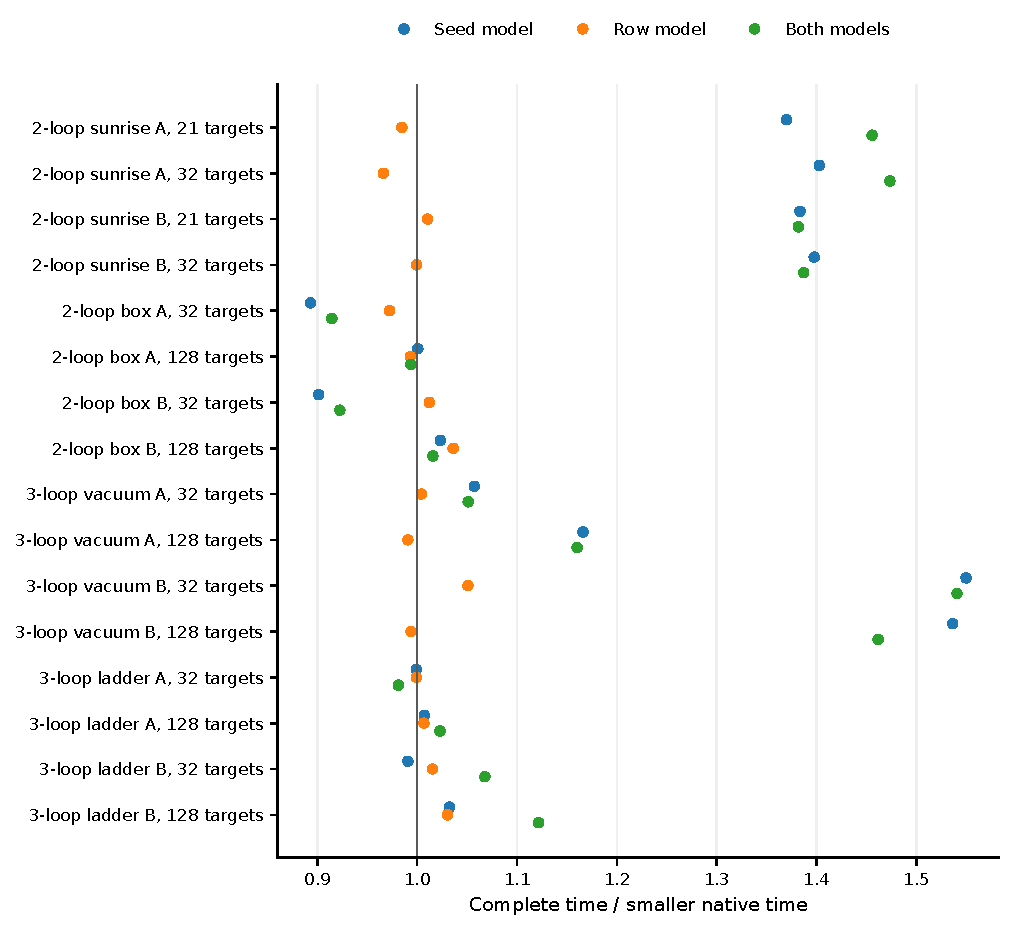
\includegraphics[width=\linewidth]{figures/integrated_runtime_times.pdf}
\caption{Median complete time for the frozen seed, row and combined policies,
divided by the smaller native control's median time on the same target batch.
Every point uses five repeated workflows with fixed physical input and master
basis. Values below one indicate lower complete time. The preceding text
states the timing boundary and profile-weighted intervals.}
\label{fig:integrated-runtime-times}
\end{figure}

\subsection{Elimination work and the contribution of each model}
A lower total runtime can come from seed generation, elimination or shared
execution changes. We therefore also inspect committed forward operations
and compare the combined method directly with the seed-only method.

The row policy relative to native choices gives an operation ratio of 0.985, a forward-stage time ratio of 1.030, and a complete-time ratio of 1.004. The operation count measures the stated coefficient-update proxy. It excludes Fermat's internal polynomial operations, while the two timing measures include the corresponding arithmetic within their stage boundaries.

The combined policy relative to the seed-only method gives an operation ratio of 0.988, a forward-stage time ratio of 1.018, and a complete-time ratio of 1.014. The operation count measures the stated coefficient-update proxy. It excludes Fermat's internal polynomial operations, while the two timing measures include the corresponding arithmetic within their stage boundaries.

The seed model's complete-time ratio to deterministic coverage is 0.978, with interval $[0.872,1.071]$. The row model's ratio to the deterministic cancellation rule is 0.985, with interval $[0.975,0.996]$. Both deterministic controls receive the same feature and runtime optimizations.

Starting from the smaller native region gives a complete-time ratio of 0.502 to the conservative native region. The combined model gives a ratio of 0.585 to that conservative control. The former comparison changes the initial native region without a learned decision. It therefore identifies a shared source of improvement that must be separated from the models' contributions.

\begin{figure}[htbp]
\centering
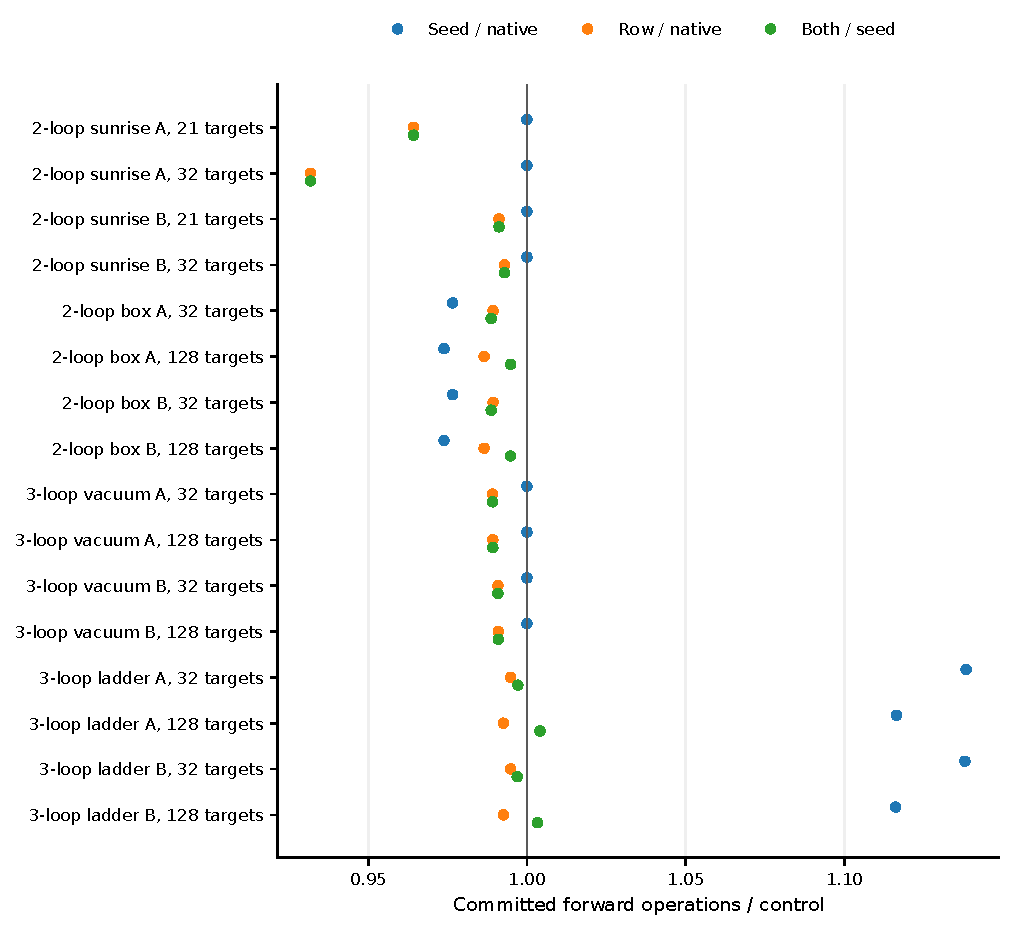
\includegraphics[width=\linewidth]{figures/integrated_runtime_operations.pdf}
\caption{Committed forward coefficient-operation ratios for the seed model
against native choices, the row model against native choices, and the
combined policy against seed selection alone. The last comparison isolates
the additional row policy within the selected seed workflow. These counts
describe the recorded update proxy and do not count internal polynomial work.}
\label{fig:integrated-runtime-operations}
\end{figure}

\subsection{Interpretation of the initial comparison}
The integrated entry point applies the settings fixed from validation.
It can run either model separately, run both models, or select the
validation-recommended method from the topology and target powers.
Automatic selection requires at least a two-percent validation improvement
over the smaller native control; otherwise it retains that control.
Unknown input classes also retain native execution. This rule avoids
paying for models on inputs where development did not support their use.
The reserved ablations above evaluate the fixed choices; reserved timings
do not change their weights or the deployment rule.

The basis check and exact coefficient comparison remain active under every
mode. Incomplete seed sets expand through the fixed fallback, and a
coefficient disagreement in the admitted basis stops the workflow.
The test uses exact rational functions of $d$ at fixed rational masses and
kinematics, with the master basis supplied in advance. Its measured times
exclude discovering and certifying a new generic symbolic basis.

The new row policies learn from complete native trajectories and act inside
Kira's changing matrix. Their allowed action is the source equation among
rows with the same leading integral. They do not choose arbitrary columns,
sectors or all mathematically possible reductions. The finite policy search,
limited physical profiles and descriptive intervals bound the conclusion:
the report establishes the measured changes on the stated inputs, while
a general gain for both models and a globally fastest reduction require
evidence beyond these comparisons.


\clearpage
\subsection{Removing redundant features in two-row decisions}
The preceding comparison lowers the row-operation count while leaving the
cost of evaluating row choices visible in the forward stage. The recorded
training data contain 1,923 groups with two source candidates among 2,520
eligible groups. Their algebra supplies an additional way to reduce this cost.

Let $\boldsymbol u$ and $\boldsymbol v$ be two rows with the same leading
integral, and let $u_p$ and $v_p$ be their nonzero leading coefficients.
The two possible elimination updates satisfy
\[
 \boldsymbol v'=\boldsymbol v-\frac{v_p}{u_p}\boldsymbol u,
 \qquad
 \boldsymbol u'=\boldsymbol u-\frac{u_p}{v_p}\boldsymbol v
              =-\frac{u_p}{v_p}\boldsymbol v'.
\]
Their nonzero positions therefore agree. The estimated number of surviving
entries and its square also agree at the finite-field points where both
leading coefficients remain nonzero. For either retained linear score, these
shared terms cancel when we compare the two candidates. The remaining
score difference is
\[
 s(S,1)-s(S,0)=
 \lambda\log\frac{1+n_1}{1+n_0}-\eta,
\]
where $S$ is the current row group, $s(S,i)$ is the score of candidate $i$,
$n_i$ is its number of nonzero entries, and candidate zero is the native
source. The quantity $\lambda$ is the coefficient of source length and $\eta$ is the
coefficient of the native-source indicator. The two retained policies use
$(\lambda,\eta)=(2,0)$ and $(1/2,-0.01)$.

When this comparison selects source zero, the implementation retains that
source without constructing cancellation features. Unsupported modular
expressions already retain the native source, so the same decision also
holds in that case. Other decisions follow the full feature calculation.
The shortcut applies only to the stated sparse linear scores, and detailed
diagnostic traces retain the full calculation.

We compare the shortcut enabled and disabled in 144 complete validation
workflows. All seventy-two pairs agree on source-choice digests, operation
counts, attempt outcomes and exact exports. The enabled path bypasses
cancellation-feature construction in 42,702 row groups. The model-weighted
ratios of decision time, forward-stage time and complete time are
0.345, 0.955 and 0.997, respectively. These ratios compare the same learned policy with and without the shortcut; they describe a reduction in inference cost without changing its algebraic choices.

A separate 4,096-entry cache for modular inverses also preserves all 144 validation reductions. Its forward-stage ratio is 1.002, its decision-time ratio is 1.024, and its complete-time ratio is 0.984. It fails the predefined forward-stage improvement criterion, so the retained implementation leaves this additional cache disabled. The original bounded cache of complete coefficient evaluations remains active.

\subsection{Confirming the reduced inference cost}
We freeze the two-row shortcut after validation and run a second comparison
on the same eight previously reserved profiles. This confirmation preserves
the model weights, seed thresholds, physical inputs, reference bases and
routing rule. It does not supply eight additional independent families.
The smaller native control, deterministic cancellation control, seed model,
row model and combined policy each receive five repetitions on all sixteen
batches, giving 400 workflows.

Every model and control uses the same new executable and temporary-storage
settings. All 400 workflows complete and match their exact reference
coefficients. They use 460 attempts, including sixty failed subset attempts
whose time contributes to the completed workflows. Their selected seed masks, committed operations, row-group
counts and native exports also agree with the corresponding initial trials.
Figure~\ref{fig:integrated-pair-times} separates complete time from the
forward stage in this confirmation~\cite{KiraIntegratedRuntimeData}.

The seed model has a complete-time ratio of 1.155 to the smaller native control, with interval $[1.024,1.316]$. The descriptive interval lies above one. Its forward-stage ratio is 1.083, with interval $[1.001,1.186]$.

The row model has a complete-time ratio of 0.999 to the smaller native control, with interval $[0.992,1.007]$. The descriptive interval includes one. Its forward-stage ratio is 1.041, with interval $[1.017,1.065]$.

The combined policy has a complete-time ratio of 1.159 to the smaller native control, with interval $[1.030,1.319]$. The descriptive interval lies above one. Its forward-stage ratio is 1.097, with interval $[1.010,1.212]$.

For the two-loop sunrise profiles, the seed, row and combined complete-time ratios are 1.397, 0.992 and 1.400. The complete-time intervals are $[1.392,1.402]$, $[0.985,0.998]$ and $[1.388,1.412]$, respectively. The row policy's forward-stage ratio is 1.044, with interval $[1.003,1.085]$.

For the two-loop box profiles, the seed, row and combined complete-time ratios are 0.964, 1.012 and 0.969. The complete-time intervals are $[0.949,0.979]$, $[1.003,1.021]$ and $[0.959,0.979]$, respectively. The row policy's forward-stage ratio is 1.028, with interval $[0.992,1.065]$.

For the three-loop vacuum profiles, the seed, row and combined complete-time ratios are 1.319, 1.003 and 1.317. The complete-time intervals are $[1.129,1.542]$, $[0.996,1.010]$ and $[1.129,1.537]$, respectively. The row policy's forward-stage ratio is 1.041, with interval $[1.007,1.078]$.

For the three-loop ladder profiles, the seed, row and combined complete-time ratios are 1.001, 0.990 and 1.010. The complete-time intervals are $[0.999,1.003]$, $[0.986,0.994]$ and $[1.003,1.017]$, respectively. The row policy's forward-stage ratio is 1.052, with interval $[1.047,1.057]$.

Applying the row policy within the learned-seed workflow gives a complete-time ratio of 1.004 to seed selection alone, with interval $[1.000,1.008]$. Its forward-stage ratio in that comparison is 1.013, with interval $[0.997,1.031]$. These measurements include the model cost and the algebraic consequences of its choices.

The row model's complete-time ratio to the deterministic cancellation rule is 0.993, with interval $[0.983,1.002]$. The deterministic rule receives the same two-row shortcut, which keeps this comparison matched.

The native integration audit verifies that every used seed belongs to the
selected mask and that each learned row attempt loads the frozen policy for
its physical class. It records 404 learned-seed attempts with 147,556 used
selected seeds, and 324 learned-row attempts with 363,759 eligible groups
and 5,795 changes from the native source. These counters show that the
models affect native equation generation and the evolving elimination.

The aggregate row-operation reduction therefore does not establish a reduction
in forward-stage time. The complete-time interval for the row policy includes
one, while always enabling seed selection or both models increases aggregate
complete time. The box cases support a conditional seed-model gain.
The automatic rule remains the rule fixed on validation; the confirmation
results do not retune it.

\begin{figure}[htbp]
\centering
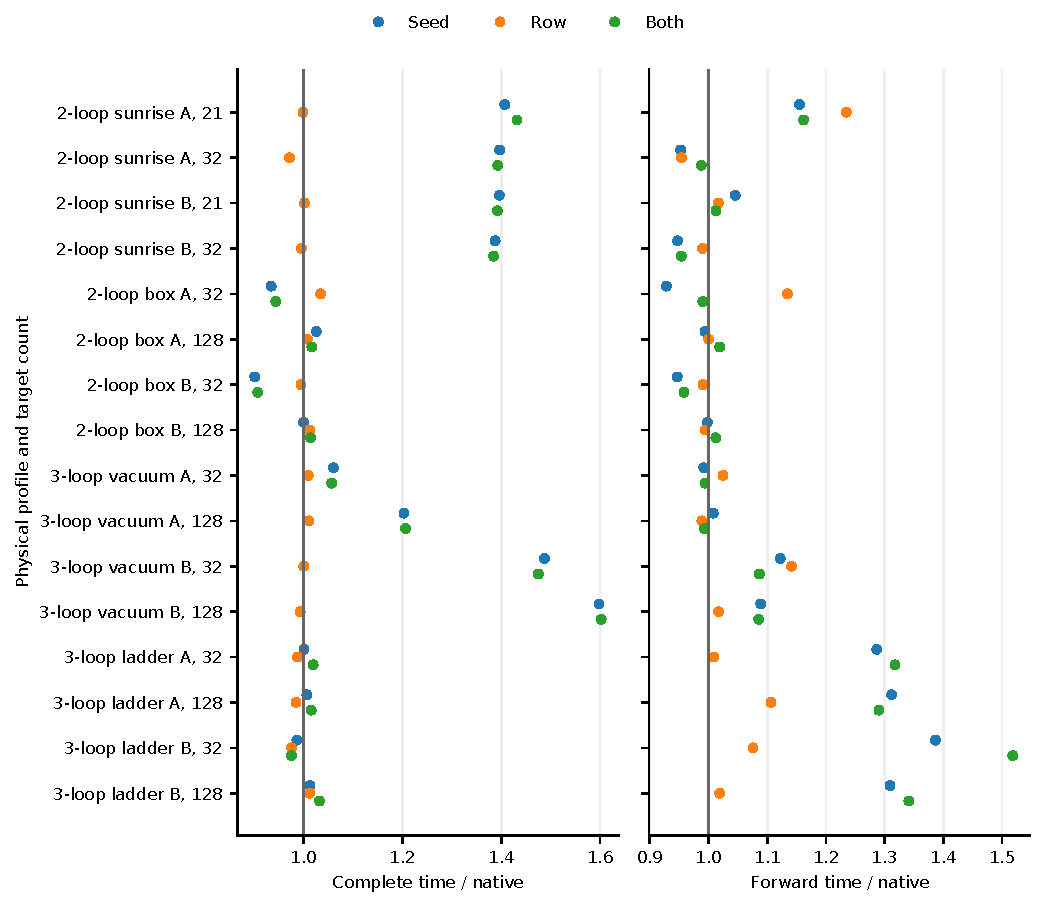
\includegraphics[width=\linewidth]{figures/integrated_pair_times.pdf}
\caption{The implementation confirmation compares the same frozen models with
the smaller native control after reducing two-row inference cost. The left
panel shows complete-time ratios and the right panel shows forward-stage
ratios. Each point uses five repeated complete reductions of the indicated
batch. The physical profiles repeat those in the initial comparison; all
algebraic choices and exact exports remain unchanged.}
\label{fig:integrated-pair-times}
\end{figure}

\clearpage
\subsection{Reducing new targets from a known master basis}
The reference answers above provide an independent benchmark check.
The production interface also accepts only the physical family, target
indices and prescribed master indices. It then determines the target
coefficients through native IBP generation and exact elimination.

To state this distinction mathematically, let $\boldsymbol I$ be the vector
of integrals in the generated system and let $A(d)$ be its IBP coefficient
matrix. The identities give $A(d)\boldsymbol I=0$. Native exact row operations
replace this system by $U(d)A(d)\boldsymbol I=0$, where $U(d)$ represents the
valid elementary row operations. Once elimination expresses all requested
targets through the prescribed masters, it gives
\[
 \boldsymbol I_{\mathcal T}=R_{\mathcal T}(d)\boldsymbol M.
\]
Here $\boldsymbol I_{\mathcal T}$ contains the requested targets,
$\boldsymbol M$ contains the supplied master integrals, and
$R_{\mathcal T}(d)$ is the rational coefficient matrix calculated by Kira.
The learned model chooses seeds and admissible source rows; the exact
identities and row operations determine this relation.

The controller checks that every target has a reduction and that every
integral on its right-hand side belongs to the supplied basis.
An additional integral triggers the fixed seed expansion. The interface
reports incompleteness if the allowed attempts fail. These checks establish
completion relative to the supplied basis under native exact IBP algebra.
They do not establish that an arbitrary supplied basis is globally minimal.
If reference coefficients are available, the interface can additionally
compare them exactly, and its records distinguish these two verification modes.

Eight application checks exercise native, seed, row, combined and automatic
execution on sunrise and box inputs. The reducer receives master indices
without target coefficients. After each run, a separate caller compares the
result with the retained exact reference, and all eight checks pass.
The application record includes input and routing time as well as the complete
reduction time. It excludes lossless evidence compression and optional common
release-integrity checks.

Automatic execution retains the routing rule fixed from validation. It enables
a learned method only in the tested feature classes where validation found
the required advantage, and uses native execution elsewhere. The individual
model modes remain available for controlled comparisons. The reported
model effects concern fixed rational kinematics, a known basis and symbolic
dimension $d$. Generic multiscale reconstruction, unrestricted higher-loop
families and global minimality remain outside this measured domain.


\clearpage
\section{Reusing model calculations without changing reductions}
\label{sec:shared-evaluation}
The preceding comparison shows that model evaluation can offset savings in
algebraic work. We therefore reduce repeated calculations inside the same
models, while retaining their weights, seed thresholds, row choices and
automatic routing rule. This section measures how the change affects both
model evaluation and the complete reduction.

\subsection{Sharing calculations in the seed network}
The seed network uses the same family and target context for every candidate.
Let $\boldsymbol c\in\mathbb R^{5h}$ be that context,
$\boldsymbol z_j\in\mathbb R^h$ the embedding of candidate seed $j$, and
$\boldsymbol a_j\in\mathbb R^h$ its attention-weighted target embedding.
The embedding dimension is $h=32$. The first score layer forms
\[
 \boldsymbol h_j=\tanh\!\left(
 W_c\boldsymbol c+W_z\boldsymbol z_j+W_a\boldsymbol a_j+\boldsymbol b
 \right),
\]
where the matrices are the corresponding blocks of the existing weight matrix,
$\boldsymbol b$ is its bias vector, and $\boldsymbol h_j$ is the hidden score
vector. The term $W_c\boldsymbol c$ is common to all candidate seeds.
We calculate its floating-point accumulator once and continue from that
accumulator for each seed. The continuation preserves the original order
of multiplications and additions.

The target-pair layer admits similar reuse. If $\boldsymbol e_i$ and
$\boldsymbol e_k$ are two target embeddings, its pair embedding is
\[
 \boldsymbol p_{ik}=\tanh\!\left(
 U_1\boldsymbol e_i+U_2\boldsymbol e_k+
 U_3(\boldsymbol e_i-\boldsymbol e_k)+
 U_4(\boldsymbol e_i\odot\boldsymbol e_k)+\boldsymbol b_p
 \right).
\]
Here $U_1,\ldots,U_4$ are blocks of the existing pair-layer matrix,
$\boldsymbol b_p$ is its bias, and $\odot$ denotes componentwise multiplication.
The first partial accumulator depends only on $i$, so we reuse it for each
allowed $k$. The remaining operations and ordered-pair aggregation keep their
original order. This removes repeated arithmetic without refitting the network.

All thirty-six development contexts give bitwise identical probability vectors
and identical masks at the six tested thresholds. The largest probability
difference is zero. The geometric mean ratio of new to preceding preparation
and inference time is 0.527. These component measurements use repeated calls with the models already
loaded; the complete-workflow comparisons below also include loading and
fallback~\cite{KiraSharedEvaluationData}.

\begin{samepage}
\subsection{Sharing cancellation estimates between source choices}
The two-row identity in the preceding section also applies to each pair
within a larger group of equations. Let $\boldsymbol R_j$ and
$\boldsymbol R_q$ be two coefficient rows whose first nonzero entries
$a_j$ and $a_q$ multiply the same integral. If both entries are nonzero,
the two possible updates give
\[
 \boldsymbol R'_j=\boldsymbol R_j-\frac{a_j}{a_q}\boldsymbol R_q,
 \qquad
 \boldsymbol R'_q=\boldsymbol R_q-\frac{a_q}{a_j}\boldsymbol R_j
             =-\frac{a_q}{a_j}\boldsymbol R'_j .
\]
The updated rows differ by a nonzero scalar and therefore contain the same
nonzero positions. Their predicted surviving-entry counts satisfy
\[
 \widehat n_{jq}=\widehat n_{qj}
\]
at the valid finite-field points used by the policy. Here $\widehat n_{jq}$
is the predicted number of entries after source $q$ updates row $j$.
The union size, cancellation count and zero-row indicator also agree in the
two directions.
\par\end{samepage}

We evaluate each unordered pair once and add its statistics to both candidate
sources. The previous implementation evaluated both directions separately.
The coefficient parser, finite-field points, cache limits and invalid-input
fallback remain the same. A further change reads fixed policy settings once
per forward-reduction stage and evaluates only nonzero score coefficients.
The policy calculates its normalized confidence when a requested decision
record uses that value. The production path retains the selected source
without calculating an unused confidence.

One thousand sparse-row checks compare all six cancellation features with
the previous implementation. All checks agree, including 210 cases with
invalid expressions or finite-field poles. Full validation then compares
the old and new implementations on six batches from the three validation
profiles. Its 180 workflows preserve probability vectors, masks, row-choice
digests, operation counts, attempt outcomes and exact exports. The validation
conditions require lower seed complete time, lower row decision time and
a row complete-time ratio no larger than $1.02$. These conditions are fixed
before validation.

\begin{samepage}
\subsection{Complete calculations with the unchanged decisions}
After validation, we freeze the implementation and compare five methods:
native choices, the seed model, the row model, both models, and automatic
routing. Each method runs with both implementations on the same sixteen
batches from the eight physical profiles in the preceding section.
Five repetitions give 800 complete workflows. We increase the confirmation
from three to five repetitions before its freeze because validation shows
execution-time variation between runs. This confirmation reuses the earlier
physical profiles and provides no additional independent-family evidence.
\par\end{samepage}

The time includes preparation, model loading, inference, fresh IBP generation,
exact elimination, back substitution, reference checks and every fallback.
The common reference calculation, interpreter launch, top-level policy lookup
and evidence compression remain outside the interval. Old and new runs
alternate within each method, and method order rotates across repetitions.
We take a median for each batch and use the same profile-weighted geometric
ratios and descriptive bootstrap intervals as before.

All 800 workflows finish with exact reference agreement, using 920 attempts. The retained failures comprise 120 unsuccessful attempts and contribute to the completed workflow times. All 400 old--new pairs preserve the recorded algebraic choices and outputs. Across validation and confirmation, the independent parser verifies 269,820 coefficient equalities through exact polynomial cross multiplication in $\mathbb Q(d)$.

The native control has a new-to-preceding complete-time ratio of 0.997, with descriptive interval $[0.960,1.030]$.

The seed model has a new-to-preceding complete-time ratio of 0.982, with descriptive interval $[0.970,0.993]$.

The row model has a new-to-preceding complete-time ratio of 1.006, with descriptive interval $[0.978,1.046]$. Its decision-time ratio is 0.669, and its forward-stage ratio is 0.977.

The combined method has a new-to-preceding complete-time ratio of 0.997, with descriptive interval $[0.976,1.015]$. Its decision-time ratio is 0.647, and its forward-stage ratio is 0.966.

The automatic method has a new-to-preceding complete-time ratio of 0.982, with descriptive interval $[0.951,1.009]$.

These comparisons isolate implementation cost while retaining each method's
decisions. Comparing the new model paths with the new native control addresses
the separate question of whether their choices repay the remaining model cost.

\begin{samepage}
Relative to the new native control, the seed model has a complete-time ratio of 1.162, with interval $[1.019,1.348]$, and a forward-stage ratio of 1.114.
\par\end{samepage}

\begin{samepage}
Relative to the new native control, the row model has a complete-time ratio of 1.023, with interval $[1.002,1.047]$, and a forward-stage ratio of 0.993.
\par\end{samepage}

\begin{samepage}
Relative to the new native control, the combined method has a complete-time ratio of 1.145, with interval $[0.998,1.334]$, and a forward-stage ratio of 1.065.
\par\end{samepage}

\begin{samepage}
Relative to the new native control, the automatic method has a complete-time ratio of 0.998, with interval $[0.948,1.049]$, and a forward-stage ratio of 0.987.
\par\end{samepage}

The seed implementation reduces the complete-time estimate by about $1.8\%$
relative to its preceding implementation, and its descriptive interval remains
below one. The row decision calculation takes about $33\%$ less time, while
the interval for complete row-model time includes one. The row comparison
therefore resolves a reduction in decision cost but does not establish a
reduction in complete time. The seed and row methods both have larger
complete-time estimates than the new native control on this set of inputs.
Automatic routing gives a ratio close to one, with an interval that spans
both a gain and a loss. These measurements support the stated implementation
savings within the tested inputs; they do not establish a general
complete-reduction advantage for the learned policies.

\begin{figure}[htbp]
\centering
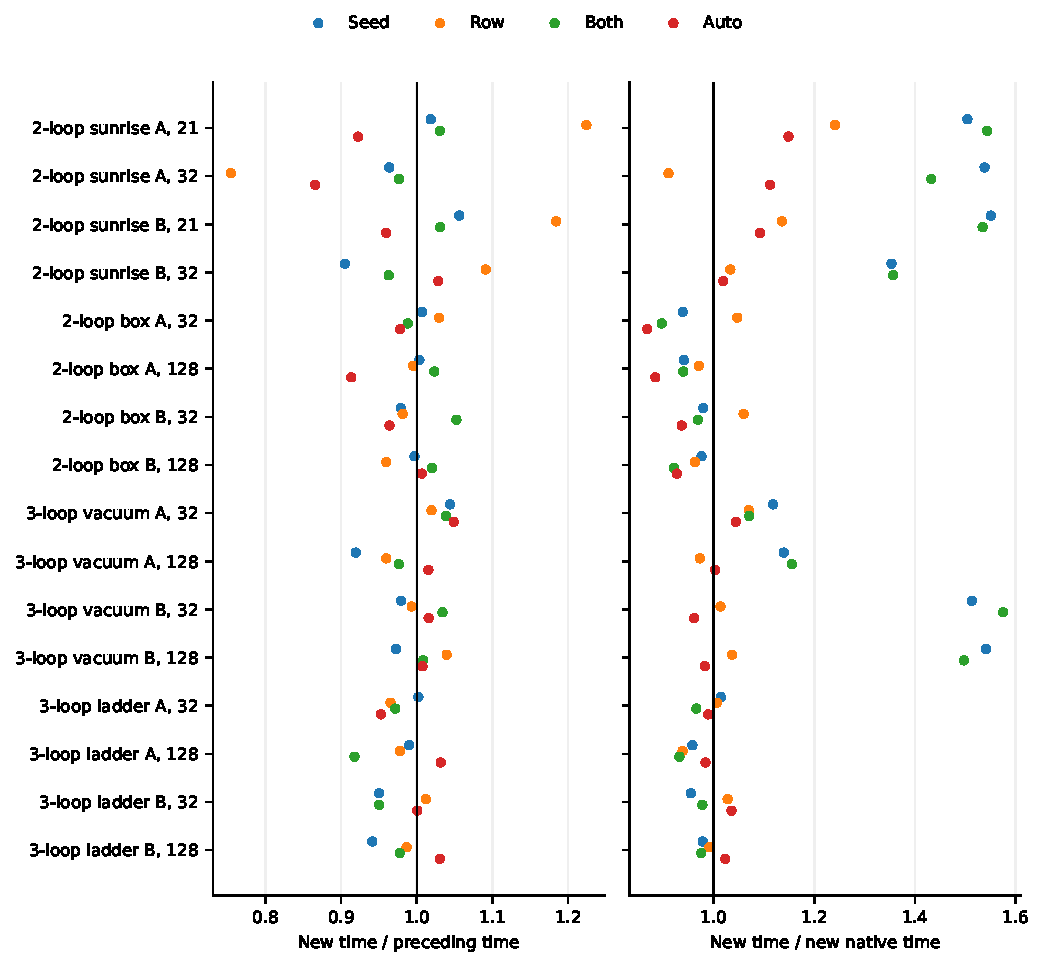
\includegraphics[width=\linewidth]{figures/shared_evaluation_times.pdf}
\caption{Complete-time ratios after sharing model calculations. The left panel
compares each method with its preceding implementation, and the right panel
compares it with the new native control. Every point uses the median of five
repetitions for one target batch. The tests keep model weights and algebraic
choices fixed, include unsuccessful attempts, and reuse the preceding eight
physical profiles.}
\label{fig:shared-evaluation}
\end{figure}

The production interface uses the shared calculations with the unchanged
validation-selected routing rule. Eight additional application checks supply
only the family, target indices and master indices to the reducer, then compare
its outputs independently with retained reference coefficients. All eight
checks pass. The original model checkpoints, preceding implementations and
negative comparisons remain available.

The operation counts are unchanged between implementations because the models
choose the same seeds and source rows. The saving comes from calculating these
choices with less repeated work. The comparison establishes measured costs for
the stated two- and three-loop inputs with fixed rational kinematics and
symbolic dimension $d$. A general gain across unrestricted higher-loop
families and a globally fastest reduction remain outside this evidence.
\clearpage


\clearpage
\section{Parallel seed evaluation and exact modular inverses}
\label{sec:parallel-inference}
The shared calculations in the preceding section reduce repeated work, but the
remaining model evaluation still contributes to the reduction time. We now
evaluate independent outputs of the seed network together and use a different
exact algorithm for modular division in the row features. We also reduce
repeated coefficient parsing and storage allocation. The weights,
thresholds, seed rules and source-row policy remain fixed, so this comparison
measures the cost of calculating the same decisions.

\subsection{Evaluating independent neural outputs together}
Let $W\in\mathbb R^{n\times m}$ be a layer's weight matrix,
$\boldsymbol x\in\mathbb R^m$ its input and $\boldsymbol b\in\mathbb R^n$
its bias. Here $m$ is the number of input components and $n$ is the number
of output components. Each output uses the partial sums
\[
 y_j^{(0)}=0,\qquad
 y_j^{(k+1)}
 =\operatorname{fl}\!\left[y_j^{(k)}
   +\operatorname{fl}(W_{jk}x_k)\right],
 \qquad k=0,\ldots,m-1 ,
\]
where $j$ identifies an output component and $\operatorname{fl}$ denotes
rounding to the existing 32-bit floating-point format. The layer then adds
$b_j$ and applies its activation when required. This expression states the
order of arithmetic used by the preceding implementation.

The previous loop finishes one output before starting the next. The new loop
advances several outputs at each input component $k$. These outputs are
independent, so the compiler can evaluate four of them with one vector
instruction while each output retains its original addition order.
We store the weights with adjacent output entries and include this
rearrangement in the model-loading cost. The shared target-context and
target-pair partial sums from the preceding section remain in use.
We retain separate multiplication and addition, the same activation functions,
and the original target aggregation order.

All thirty-six development contexts give bitwise identical probability
vectors. The selected masks also agree at all six tested thresholds.
The geometric mean ratio of new to preceding preparation and inference
time is 0.423. This component comparison uses five alternating
repetitions with loaded models. The complete reductions below include loading
and the weight rearrangement.

\subsection{Computing modular inverses with Euclid's algorithm}
The row policy evaluates rational coefficients at the same two finite-field
points as before. Division by a nonzero field element $a$ requires its
inverse modulo the prime $p=2^{31}-1$. The preceding implementation uses
$a^{-1}=a^{p-2}\bmod p$. The extended Euclidean algorithm gives integers
$x$ and $y$ such that
\[
 ax+py=1,\qquad a^{-1}=x\bmod p .
\]
Here $x$ supplies the inverse because the greatest common divisor of $a$
and $p$ is one. The algorithm repeatedly divides the current integer
remainders and updates the coefficients of $a$ and $p$ until it reaches
that greatest common divisor.

We use this inverse in the same coefficient parser, including negative
integer powers. The prime, evaluation points, cache bounds and
unordered-pair cancellation estimates remain unchanged. A zero denominator
still rejects that estimate and retains the existing fallback. These
finite-field calculations guide the row choice; native Kira performs
the symbolic row operations.

\begin{samepage}
Integer coefficients have the same residue at both dimension points.
For a coefficient $c\in\mathbb Z$, we calculate its residue $r$ once,
\[
 r=c\bmod p,\qquad (c(17),c(19))=(r,r)\quad\text{in }\mathbb F_p^2.
\]
Here the two entries are the coefficient values used in the cancellation
test, and $\mathbb F_p$ is the field of integers modulo $p$. For short
integer expressions, this removes two general expression evaluations and
the cache lookup. Other expressions retain the bounded parser and cache.
We also allocate the evaluated coefficients for a row group in one
contiguous array, which removes separate allocations for each row.
These changes preserve every coefficient value and the order of the
cancellation calculations.
\par\end{samepage}

Checks on 100,000 nonzero field elements agree with the preceding inverse
and satisfy $aa^{-1}=1\bmod p$. A further 1,000 sparse-row checks agree
on all six features, including the 210 cases with invalid expressions or
finite-field poles. Five alternating repetitions give a ratio of 0.803 for new to preceding row-feature calculation
time with cleared coefficient caches. The complete reductions also exercise
the ordinary cache reuse and source-selection code.

\subsection{Complete reduction costs and exact checks}
We first tested the Euclidean inverse alone with the parallel seed
calculation. Its 144 validation workflows preserved all decisions and exact
exports, but its complete row-time ratio was $1.027$ and its row-decision
ratio was $1.017$. Both missed the conditions stated below, so we retain
this candidate as a rejected development result. The revised candidate
adds the integer evaluation and contiguous storage described above.
These changes use development and validation inputs; confirmation results
do not select them.

The next 144 validation workflows compare native choices, seed selection,
row selection and both learned choices on six batches from three physical
profiles. We fix the adoption conditions before validation and require
identical decisions and exports, lower seed complete time, lower row
decision time and a row complete-time ratio at most $1.02$.
Both component comparisons must also improve.

After validation, we freeze the implementation and run the same four methods
on sixteen batches from the eight physical profiles used in the preceding
comparison. Five repetitions with each implementation give 640 workflows.
These inputs provide a repeated implementation comparison and add no new
independent-family evidence. Model weights and thresholds remain fixed.

Timing includes preparation, loading, prediction, fresh IBP generation,
exact elimination, back substitution, reference checks and every fallback.
Reference preparation, interpreter launch, release-hash verification,
policy lookup and evidence
compression remain outside the timed interval. We alternate the implementations
within each method and rotate method order. We take the median for each batch
and report the same profile-weighted geometric ratios and descriptive
95\% bootstrap intervals as before. A ratio below one means less time.
The internal decision timer covers completed policy paths. The complete
workflow timer also includes feature evaluations that return an invalid
estimate and retain the native source.

All 640 workflows pass the exact reference check, using 760 attempts, including 120 unsuccessful attempts. All 320 old--new pairs preserve probability vectors, selected seeds, row-choice digests, committed operations and exact exports. The independent audit verifies 215,856 coefficient equalities over $\mathbb Q(d)$ across the 784 validation and confirmation workflows~\cite{KiraParallelInferenceData}.

\begin{samepage}
The native control has a new-to-preceding complete-time ratio of 1.005, with descriptive interval $[0.976,1.035]$.
\par\end{samepage}

\begin{samepage}
The seed model has a new-to-preceding complete-time ratio of 0.990, with descriptive interval $[0.977,1.003]$.
\par\end{samepage}

\begin{samepage}
The row model has a new-to-preceding complete-time ratio of 0.990, with descriptive interval $[0.971,1.010]$. Its decision-time ratio is 0.791, and its forward-stage ratio is 0.998.
\par\end{samepage}

\begin{samepage}
The combined method has a new-to-preceding complete-time ratio of 0.984, with descriptive interval $[0.965,1.007]$. Its decision-time ratio is 0.816, and its forward-stage ratio is 1.039.
\par\end{samepage}

The new native control provides a separate comparison for the cost and benefit of the learned decisions. It uses the same execution settings and exact checks.

\begin{samepage}
Relative to that control, the seed model has a complete-time ratio of 1.096, with interval $[0.963,1.275]$.
\par\end{samepage}

\begin{samepage}
Relative to that control, the row model has a complete-time ratio of 0.982, with interval $[0.959,1.003]$.
\par\end{samepage}

\begin{samepage}
Relative to that control, the combined method has a complete-time ratio of 1.100, with interval $[0.966,1.279]$.
\par\end{samepage}

All three new-to-preceding complete-time intervals include one. The component timings show lower evaluation cost, while these complete-workflow measurements leave the size of the overall change uncertain. Relative to native choices, the aggregate seed and combined ratios exceed one, and the row-only interval also includes one. The results therefore support lower model-evaluation cost within the measured scope; a general complete-time advantage over native Kira remains unestablished.

For the seed method, the complete-time ratios relative to native choices are 0.911 for the double boxes, 0.935 for the three-loop ladders, 1.380 for the sunrise integrals and 1.226 for the three-loop vacuum integrals.

For the row method, the complete-time ratios relative to native choices are 1.011 for the double boxes, 0.958 for the three-loop ladders, 0.962 for the sunrise integrals and 0.999 for the three-loop vacuum integrals.

For the combined method, the complete-time ratios relative to native choices are 0.902 for the double boxes, 0.945 for the three-loop ladders, 1.394 for the sunrise integrals and 1.232 for the three-loop vacuum integrals.

\begin{figure}[htbp]
\centering
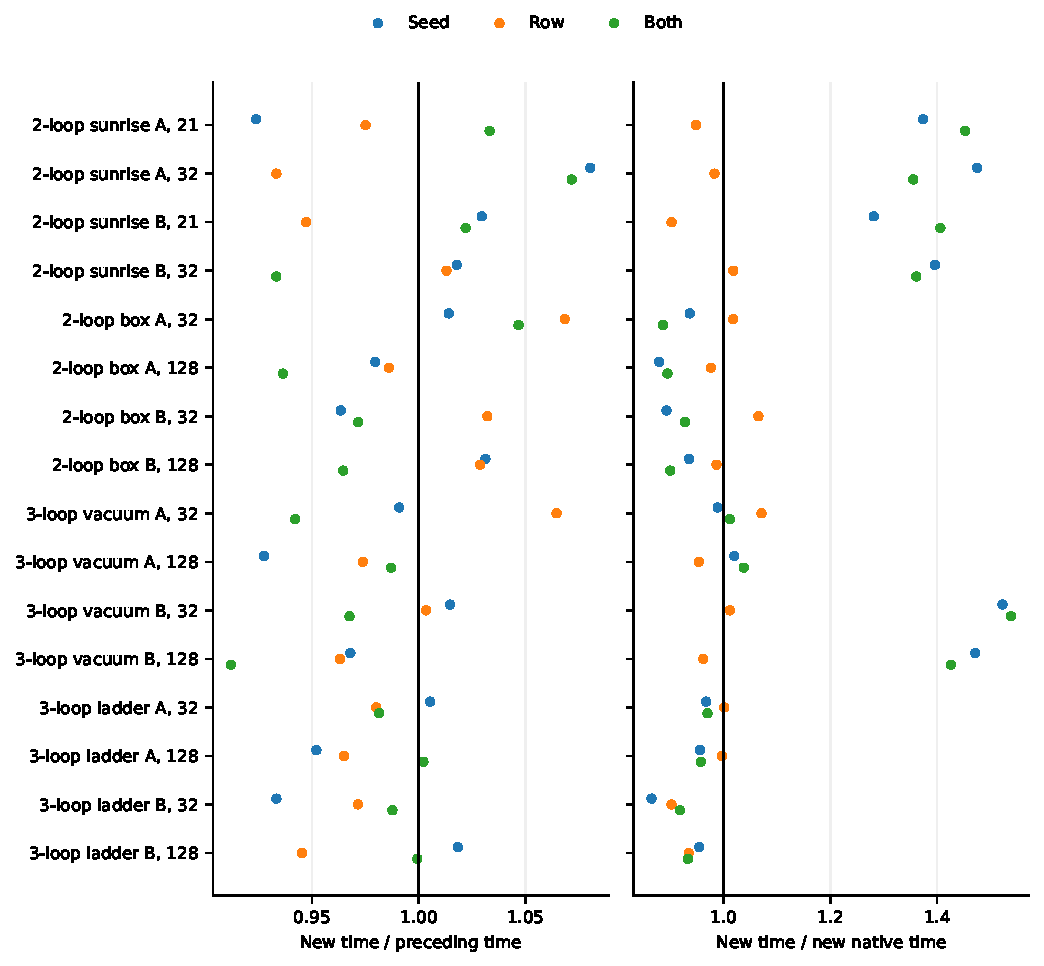
\includegraphics[width=\linewidth]{figures/parallel_inference_times.pdf}
\caption{Complete reduction times for the unchanged learned policies. The left
panel compares the new implementation with the preceding shared calculations.
The right panel compares each new method with the new native control.
Each point is the median of five repetitions for one target batch, including
failed attempts and fallback. A and B identify the two physical profiles
within each topology, and the numbers give the target counts.}
\label{fig:parallel-inference}
\end{figure}

Eight further application checks supply family definitions, targets and
master indices without supplying target coefficients. Independent comparisons
after execution pass in all eight cases. The production interface uses the
validated implementation with the unchanged routing rule.

The algebraic operation counts remain fixed between the two implementations.
The time change comes from evaluating the same model decisions with different
arithmetic. This distinguishes a reduction in model cost from a reduction in
the algebra needed by Kira. The comparisons concern two- and three-loop
inputs with fixed rational kinematics and symbolic dimension $d$; they do
not establish a general speed advantage across unrestricted higher-loop
or multiscale reductions.
\clearpage


\clearpage
\section{Target-dependent equation selection}
\label{sec:equation-selection}
The preceding policies choose seeds and source rows, but each retained seed
can produce several identities. A third model selects identities for the
requested targets before Kira performs modular independence elimination.
This choice can reduce the system that Kira processes, provided that the
saved algebraic work exceeds the cost of making the choice. We therefore
measure equation preparation and the complete reduction with the model
included~\cite{Kira3,KiraEquationSelectionData}.

\subsection{The equations and their training labels}
Let $\mathcal T$ be the set of requested integral indices. An identity
generated from seed $\boldsymbol\sigma$ and derivative or
Lorentz-invariance operator $o$ has the form
\begin{equation}
 E_{\boldsymbol\sigma,o}:\qquad
 \sum_{\boldsymbol a\in A_{\boldsymbol\sigma,o}}
 c_{\boldsymbol\sigma,o,\boldsymbol a}(\boldsymbol x,d)
 I_{\boldsymbol a}=0 .
 \label{eq:equation-selection-identity}
\end{equation}
Here $A_{\boldsymbol\sigma,o}$ is the set of integral indices that occur
in the identity and $c_{\boldsymbol\sigma,o,\boldsymbol a}$ is the
coefficient of $I_{\boldsymbol a}$. The variables $\boldsymbol x$ and
$d$ retain their definitions as the kinematic parameters and integration
dimension. The operator index distinguishes the several identities from
one seed, so the third policy can retain only part of a seed's output.

We first run native Kira reductions on training families and record the
integral supports of the equations retained in the final regenerated
system. An integral support is the set of indices with nonzero
coefficients after combining repeated terms at the finite-field selection
point. If $\mathcal S_{\rm native}$ is the collection of these supports,
the training label is
\begin{equation}
 y_{\boldsymbol\sigma,o}
 =\mathbf 1\!\left[
  \operatorname{supp}(E_{\boldsymbol\sigma,o})
  \in\mathcal S_{\rm native}\right].
 \label{eq:equation-selection-label}
\end{equation}
The indicator $\mathbf 1$ equals one when the condition holds and zero
otherwise. Several equations can have the same support and different
coefficients, so this label describes support membership in the recorded
selection. It supplies a conservative training proxy and does not establish
a necessary or smallest equation set.

The training collection contains 74,692 candidate equations, with
5,978 positive labels, from ten target batches in six physical profiles.
These profiles comprise two-loop sunrise and double-box integrals and
three-loop vacuum integrals. We keep three additional profiles for
validation and eight for testing. The held-out tests also include a
three-loop ladder topology absent from the training and validation
collections. Each profile fixes rational masses and kinematic invariants,
while the reductions retain symbolic dependence on $d$.

\subsection{Features and the learned probability}
The model receives 23 numerical features that describe the family,
the target set, the seed and the generated equation. These features include
the numbers of loops and external momenta, the number of integral indices,
the target count, positive propagator powers, numerator powers, sector
membership, the operator index and the equation's integral terms.
For example, the distance from a seed to the targets is
\begin{equation}
 \delta(\boldsymbol\sigma,\mathcal T)
 =\min_{\boldsymbol a\in\mathcal T}
   \sum_{i=1}^{N}|\sigma_i-a_i| ,
 \label{eq:equation-selection-distance}
\end{equation}
where $N$ is the number of expressions in the integral family.
The model also uses differences between the seed's dot or numerator
counts and the largest corresponding counts in the target set and
in the same sector. These quantities describe which equations lie near
the requested part of the integral-index lattice.

We fit a classification tree using weighted impurity reduction,
with equal total weight for each training profile~\cite{CART1984}.
A sequence of feature comparisons leads to a leaf, which stores
\begin{equation}
 p_{\boldsymbol\sigma,o}
 =\frac{n_+ + 1/2}{n_{\rm leaf}+1},
 \qquad
 E_{\boldsymbol\sigma,o}\ \hbox{is retained if}\
 p_{\boldsymbol\sigma,o}\geq\tau .
 \label{eq:equation-selection-probability}
\end{equation}
Here $n_+$ is the number of positive training rows in that leaf,
$n_{\rm leaf}$ is its total number of training rows and $\tau$ is
the retention threshold. The fitted tree has 233 nodes and a maximum
depth of eight. Each accepted split leaves at least 24 rows in each
child. The score is a smoothed empirical frequency of the recorded
label, and its numerical value has no separate calibration guarantee.

Training the tree takes 2.75 seconds after the native examples have
been collected. This time excludes the generation of training reductions.
We retain one additional diagnostic field for coefficient-text length,
but exclude it from the decisions because equivalent coefficient
expressions can have different printed lengths. The saved model and
its compiled evaluator give identical probabilities for 18,754 candidates
in the implementation checks.

\subsection{Native integration and the cost of a decision}
Kira constructs a candidate identity before the model first scores it.
The retained identities then enter native modular equation processing.
Symmetry identities and preferred-basis relations continue through their
existing paths. The model scores the IBP and Lorentz-invariance identities
at the generation interface; it does not replace Kira's later algebraic
independence checks.

Several operators share one seed, so we calculate their common
seed-to-target features once. We also store each seed--operator decision.
When Kira later requests the same identity, a stored omission allows the
generation code to skip rebuilding its coefficients. A retained identity
is regenerated through the native code. The tree also calculates an equation feature only when a comparison
on its chosen path needs that feature. Propagator and numerator counts
come directly from the native integral ordering. These saved decisions avoid
repeated predictions and remove part of the repeated equation generation.
Exact comparisons check that the implementation changes preserve the
decision features, probabilities, masks and reduction results.

After reduction, we require every target to lie in the prescribed master
basis. An incomplete filtered attempt triggers an unfiltered native
attempt, followed by an enlarged native seed range when necessary.
The benchmark additionally compares every exported rational coefficient
with an independently stored native reference. The application interface
requires the master basis and can operate without reference target
coefficients; we check these application outputs separately after the
reducer returns.

\subsection{Validation and held-out comparisons}
We select thresholds using complete reduction times on the three
validation profiles. A topology uses the learned filter in the automatic
route only when its validation time ratio is below $0.98$; other
topologies retain native equation choices. The test also includes a
forced learned filter and a deterministic distance filter using
Eq.~\eqref{eq:equation-selection-distance}. Validation selects each
filter's threshold before the test runs, and the saved hashes fix the
model, integration and test protocol.

The test contains fourteen target batches from eight physical profiles.
Each sunrise batch contains 21 targets; the other profiles use batches
of 32 and 128 targets. Five alternating repetitions compare native choices,
the forced learned filter, the distance filter and the automatic route,
giving 280 complete workflows. All four arms use the same compiled
binary, with native choices switching off the three learned policies.
Each time includes preparation, loading,
predictions, equation generation, exact algebra, output checks and all
failed attempts before fallback. The experiment driver is already running when timing begins; Kira process startup and model loading are included. Creation of the independent references
and compression of the evidence files lie outside this timer.

Equation preparation includes generation with modular processing,
equation selection, modular solving and equation regeneration.
It therefore measures the full preparation affected by the filter.
We report median times within each batch and geometric ratios with equal
weight for each physical profile. Descriptive intervals resample these
eight profiles 10,000 times. These intervals describe this finite set of
profiles and do not establish performance for arbitrary multiloop families.

\subsection{Results and scope}
The validation route is double box: off, sunrise: learned at $\tau=0.001$, vacuum3: learned at $\tau=0.0001$. Other topologies use native equation choices. The forced learned filter uses $\tau=0.001$, while the distance filter retains seeds with $\delta\leq 4$. These choices remain fixed throughout the held-out tests.

All 280 complete workflows reproduce their native reference coefficients. The independent audit checks 91,240 coefficient pairs, including 1,931 distinct expression pairs, by exact rational simplification in $d$. The workflows contain 40 failed filtered attempts before successful fallback, and their times include these attempts. Native median complete times range from 0.785 to 5.880 seconds across the fourteen batches.

The forced learned filter has a complete-time ratio of 1.080, with descriptive interval $[0.976,1.220]$. Its equation-preparation ratio is 1.053, with descriptive interval $[0.904,1.224]$. The generated-equation ratio is 0.769, and the selected-equation ratio is 0.985. All ratios use the matched native control, so a value below one indicates a lower measured cost.

The distance filter has a complete-time ratio of 1.016, with descriptive interval $[0.994,1.040]$. Its equation-preparation ratio is 1.089, with descriptive interval $[1.035,1.144]$. The generated-equation ratio is 1.000, and the selected-equation ratio is 1.000. All ratios use the matched native control, so a value below one indicates a lower measured cost.

The automatic route has a complete-time ratio of 1.098, with descriptive interval $[0.981,1.259]$. Its equation-preparation ratio is 1.062, with descriptive interval $[0.896,1.261]$. The generated-equation ratio is 0.849, and the selected-equation ratio is 1.000. All ratios use the matched native control, so a value below one indicates a lower measured cost.

The automatic route does not lower the aggregate complete time in this test. Equation-count changes therefore do not establish an overall runtime gain.

\begin{figure}[htbp]
 \centering
 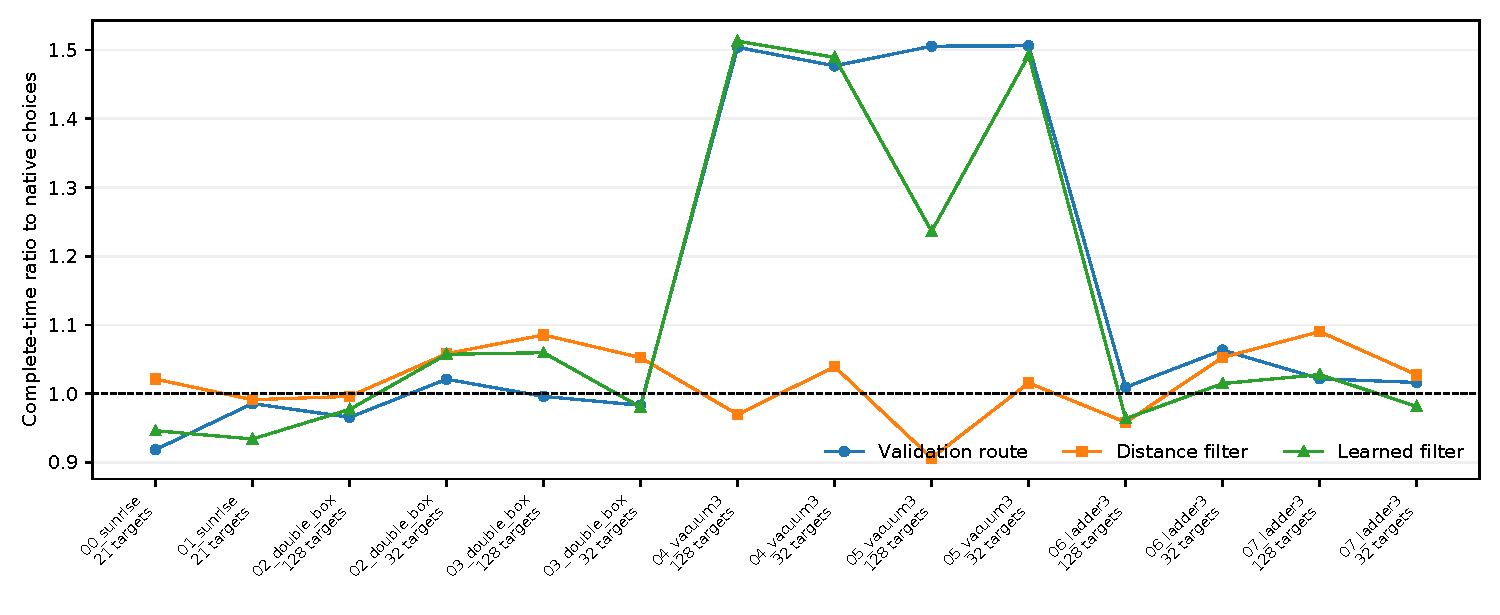
\includegraphics[width=\textwidth]{figures/equation_complete_times.pdf}
 \caption{Median complete-time ratios for the fourteen held-out batches.
 Each point uses five repetitions and includes checks and fallback.
 The dashed line is the native control.}
 \label{fig:equation-complete}
\end{figure}
\begin{figure}[htbp]
 \centering
 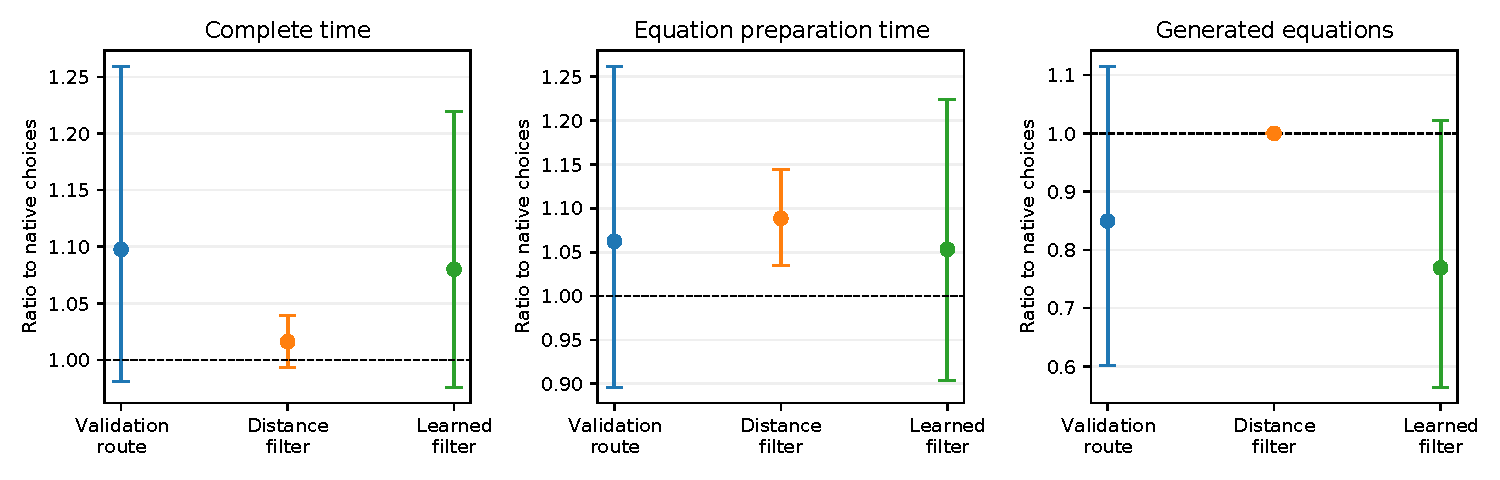
\includegraphics[width=\textwidth]{figures/equation_aggregate_costs.pdf}
 \caption{Profile-weighted geometric ratios of complete time, equation
 preparation time and generated-equation count. Bars show descriptive
 intervals from resampling the eight physical profiles.}
 \label{fig:equation-aggregate}
\end{figure}

After freezing the model, we also collect 77,246 held-out candidate labels, with 6,932 positive labels. At the forced learned threshold, precision is 11.33\% and recall is 95.63\%, with mean squared probability error 0.0621. These quantities measure agreement with the native support-membership proxy. Exact coefficient comparisons measure the validity of the resulting reductions.

\begin{figure}[htbp]
 \centering
 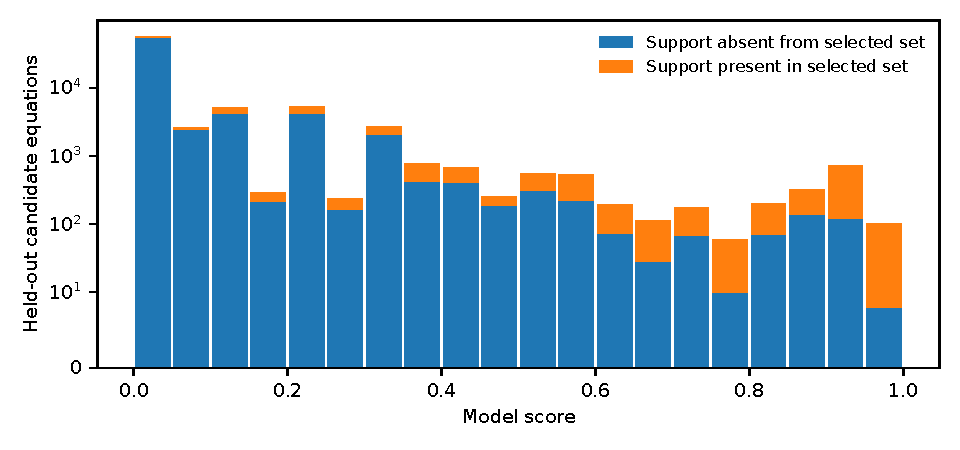
\includegraphics[width=.78\textwidth]{figures/equation_label_scores.pdf}
 \caption{Held-out model scores grouped by the native support-membership
 label. The vertical scale is linear near zero and logarithmic above ten
 equations. The labels describe selected supports rather than necessary
 equations.}
 \label{fig:equation-labels}
\end{figure}

A further 48 complete workflows test the equation route together with the existing row policy and with both existing policies on four profiles. Adding the equation route gives a complete-time ratio of 1.165 to the row-only configuration and 1.184 to the configuration with both earlier models. These comparisons use three repetitions and retain all fallback costs. All pass the reference checks. Eight application runs also pass exact coefficient comparisons after execution with reference coefficients withheld from the reducer.

The early full-feature implementation and subsequent feature-sharing implementations remain in the evidence collection, including their slower results. The final comparison uses the frozen implementation selected before held-out testing. Its performance depends on target size, topology and the cost of generating and reducing the retained equations. The experiment covers physical two- and three-loop reductions at fixed rational kinematics with symbolic $d$; it does not establish gains on arbitrary higher-loop or fully multiscale problems~\cite{KiraEquationSelectionData}.
\FloatBarrier

\subsection{The domain selected before testing}
Validation enables the equation model for the sunrise and three-loop vacuum topologies. This identifies four of the eight test profiles before any test timing is available. On these profiles, the automatic route has a complete-time ratio of 1.194, with descriptive interval $[0.951,1.498]$. Its equation-preparation ratio is 1.078, with descriptive interval $[0.765,1.519]$. The corresponding generated-equation ratio is 0.722.

For sunrise profiles, the automatic complete-time ratio is 0.951 and the preparation ratio is 0.765. For vacuum3 profiles, the automatic complete-time ratio is 1.498 and the preparation ratio is 1.519. For double box profiles, the automatic complete-time ratio is 0.991 and the preparation ratio is 0.988. For ladder3 profiles, the automatic complete-time ratio is 1.027 and the preparation ratio is 1.110. The double-box and ladder routes retain native equation choices, so differences between their automatic and native timings mainly reflect repeated-run variation and routing overhead. The all-profile comparison remains the primary result; these fixed-domain results state where the learned filter was active.



\clearpage
\subsection{Restricted deployment and fresh confirmation}
The broad test exposes incomplete equation filters in the new vacuum
profiles. Their native fallback retains exact results and adds cost.
We therefore fix a restricted deployment using the same trained tree.
It enables the equation filter at $\tau=0.001$ for the recorded
21-target sunrise batches and retains native equation choices for
other topologies and target sets. The broader test supplies development
evidence for this deployment revision.

Each supported batch contains the top-sector scalar integral and its
one-dot and one-numerator variants, together with the corresponding
integrals in the three two-propagator sectors. This gives 21 targets
whose index vectors are fixed in the deployment definition.
We reserve six additional mass and momentum profiles before running
their reductions. None of these profiles occurs in the preceding
training, validation or broad-test sets. Their squared masses and
external invariant are fixed rational numbers, while $d$ remains symbolic.
The tree, threshold, target domain and new profile definitions are
fixed before this confirmation begins.

Nine alternating repetitions compare the learned filter, native choices
and the previously selected distance control in each profile. These
162 complete workflows use the same timing and exact-check rules
as the preceding test, including every failed attempt.

The learned filter has a complete-time ratio of 0.994, with descriptive interval $[0.991,0.997]$ and an equation-preparation ratio of 0.785, with descriptive interval $[0.776,0.794]$. Its generated-equation ratio is 0.414, and its selected-equation ratio is 1.000. The distance control has a complete-time ratio of 1.003, with descriptive interval $[1.000,1.006]$.

The complete-time interval remains below one for these six profiles, supporting a measured gain within the restricted domain.

A further 36 workflows compare the existing seed and row policies with the configuration that also includes the equation filter. Adding the third model gives a complete-time ratio of 1.317, with descriptive interval $[1.296,1.337]$ and a preparation ratio of 1.151, with descriptive interval $[1.136,1.168]$ to the two-model configuration. This comparison uses three repetitions in each of the six profiles.

All 162 main workflows, 36 composition workflows and six basis-only applications pass the independent exact audit, which checks 7,582 coefficient pairs. The 204 workflows include 54 failed attempts. The six applications receive the prescribed masters without reference target coefficients, and their outputs pass coefficient comparisons after execution.

Native median complete times range from 0.692 to 0.709 seconds in these six profiles. The geometric mean preparation fraction of native complete time is 3.29\%. This small fraction explains why the reduction in preparation time produces a smaller change in complete time. The main confirmation has zero failed attempts; all 54 failed attempts in its extended audit arise in the composition comparisons.

\begin{figure}[htbp]
 \centering
 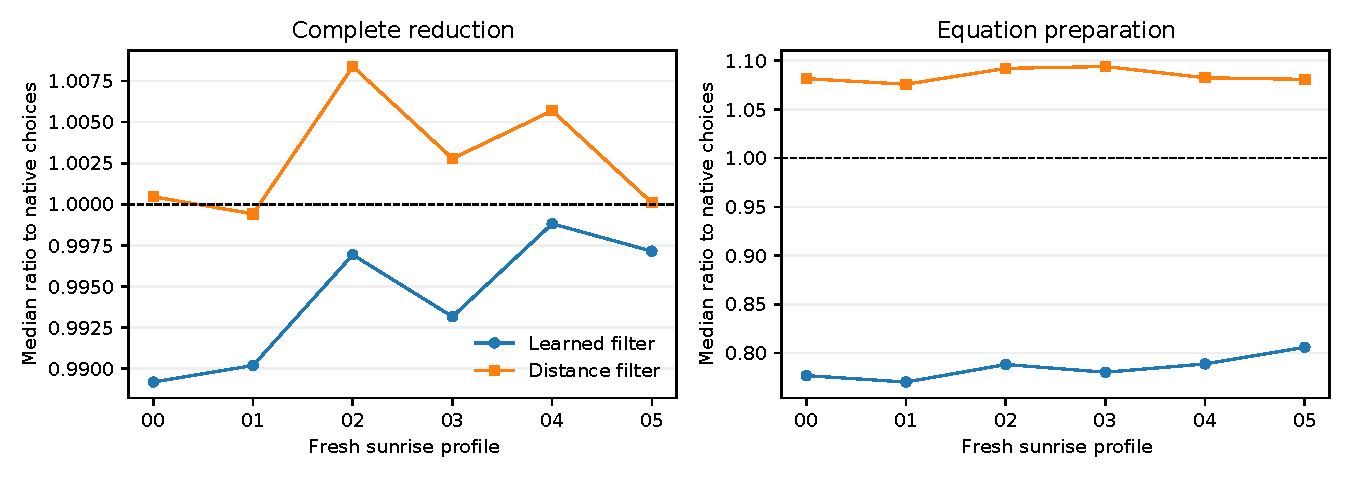
\includegraphics[width=\textwidth]{figures/equation_confirmed_costs.pdf}
 \caption{Fresh confirmation of the restricted sunrise deployment.
 Each profile uses nine repetitions for each method. Complete and
 preparation times include prediction and fallback costs.}
 \label{fig:equation-confirmed}
\end{figure}
The application interface enables this equation policy when it runs with native seed and row choices. Requests for either earlier learned policy retain native equation choices. This guard avoids the slower measured three-model combination.
The broader initial route and its slower vacuum results remain available
as experimental evidence. The measured domain contains two-loop sunrise
integrals with the stated target set, and extension to other target sets
or topologies requires further independent evidence~\cite{KiraEquationSelectionData}.
\FloatBarrier

\clearpage
\subsection{Predicting equations before constructing their coefficients}
\label{sec:early-equation-selection}
The preceding equation model first inspects a constructed identity, so its
initial prediction still requires that identity's coefficients. To reduce
this cost, we train a new version of the same model that uses only the seed,
the operator and the requested targets. This moves the decision to the point
where Kira can avoid constructing an omitted identity.

A diagnostic study motivates this change. In twelve exact native runs,
equation preparation forms the largest recorded block in the 128-target
three-loop ladder reductions. The two ladder profiles have median
preparation intervals of 1.41 and 1.23 seconds, within complete times of
4.23 and 4.36 seconds. Initial family preparation and equation preparation
together account for about 54--55\% of those times. These diagnostic
intervals come from logged stage boundaries and include wrapper costs;
the final comparison below uses the internal timers defined for this study.

For the identity in Eq.~\eqref{eq:equation-selection-identity}, the new
decision has the form
\begin{equation}
 \widehat p_{\boldsymbol\sigma,o}
 =f_\theta\!\left(\phi(\boldsymbol\sigma,o,\mathcal T)\right),
 \qquad
 \widehat p_{\boldsymbol\sigma,o}\geq\tau
 \ \Longrightarrow\ E_{\boldsymbol\sigma,o}\ \hbox{is constructed}.
 \label{eq:early-equation-decision}
\end{equation}
Here $\phi$ is the vector of features available before construction,
$f_\theta$ is the classification tree with trained parameters $\theta$,
and $\tau$ is the retention threshold. The 17 features describe the
numbers of loops, external momenta and indices, the target count, the
seed's sector, dots and numerator rank, their differences from target
limits, the distance in Eq.~\eqref{eq:equation-selection-distance},
whether the seed is itself a target, and the operator index.
The tree therefore has no need to inspect the equation's coefficients
or integral terms.

Kira supplies the ordered IBP operators, and the integration retains their
positions when it omits an equation. Several operators share the same seed
features, so we calculate those features once and store the decision for
each seed--operator pair. Kira constructs accepted equations through its
native algebra and reuses the stored decisions during later regeneration.
Symmetry identities and preferred-basis relations retain their existing
treatment. This placement reduces both repeated model work and the initial
construction of identities that the model rejects.

We retain the support-membership labels in
Eq.~\eqref{eq:equation-selection-label} and add four training batches from
two new ladder profiles. The combined collection contains 153,124 candidate
equations, including 12,270 positive labels, in fourteen batches from
eight physical profiles. These profiles contain the two-loop sunrise and
double-box and the three-loop vacuum and ladder structures. We fit trees
with maximum depths eight and twelve, using equal total weight per profile
and the same smoothed leaf frequency as before~\cite{CART1984}.
The trees contain 295 and 1,335 nodes and take 3.39 and 5.85 seconds to fit
after collection of the native training reductions. Their splits leave at least
24 and eight rows in each child, respectively. A separate implementation
check compares 918,744 decisions and finds agreement between the
stored Python features and the C++ evaluator's recomputed seed features.

The training label still describes membership in a recorded native equation
selection. It supplies neither a smallest sufficient equation set nor a
calibrated completeness probability. Kira therefore checks whether the
result expresses each target in the prescribed master basis. If the
filtered equations are insufficient, the application retries native
equations and then a larger native seed region. Exact algebra determines
all coefficients, and the benchmark additionally compares them with an
independent native reduction.

\subsection{Selecting the complete calculation on validation profiles}
We compare both trees at thresholds 0.001, 0.003 and 0.01 with native
choices and a distance filter. Repeated validation requires at least
1\% lower complete time, at least 5\% lower equation-preparation time
and no fallback before activating an early filter. We then measure
combinations with the existing seed and row models. An additional model
must lower complete time by at least 1\% relative to early filtering
alone and require no fallback in validation.

The validation record contains 77 initial candidate and control workflows,
84 repeated candidate workflows, 72 row-composition workflows and
96 seed-composition workflows. A second vacuum profile checks another
mass pattern in the composition stage. Adding the row model gives less
than 1\% incremental saving in the ladder and vacuum comparisons and
increases double-box time. Seed combinations require extra attempts for
some larger double-box and vacuum batches. These costs remain in the
comparisons and prevent those combinations from meeting the activation rule.

Validation therefore selects the depth-twelve tree for double-box batches
and the depth-eight tree for vacuum and ladder batches, with $\tau=0.01$.
The final route retains native seed and row choices. It keeps the preceding
equation policy for the recorded 21-target sunrise batch, where early
filtering fails the validation activation rule. Other structures and
ordered target lists use the preceding guarded route. This selection
minimizes measured cost among the eligible validation candidates; it does
not establish a globally fastest reduction.

We preserve an excluded preliminary collection whose proposed additional
profiles overlapped earlier reserved definitions. We replace those profiles
before the final collection and exclude every provisional row, model and
outcome from the results above. The final training, validation and test
profiles are distinct. They can share topologies, target indices and
lower-sector integral structure.

\subsection{Independent complete-reduction comparison}
We fix the models, integration, thresholds and target domains before testing
eight additional physical profiles. Two profiles belong to each of the
sunrise, double-box, vacuum and ladder structures. Sunrise uses 21 targets,
and each remaining profile uses batches of 32 and 128 targets.
Five alternating repetitions compare native choices, the preceding release,
the deployed early policy and the validation-selected distance filter.
This gives 280 complete comparison workflows. The same new binary runs
the native, early and distance arms; the preceding release uses its saved
binary and policy. The native control includes the existing project
runtime improvements and switches off learned choices.

The profiles fix rational squared masses and external invariants, while
$d$ remains symbolic. The sunrise squared masses are $(2,7,11)$ and
$(3,7,13)$, with $p^2=-101$ and $-103$, respectively.
The double-box pairs are $(s,t)=(-101,-103)$ and $(-107,-109)$.
The vacuum squared-mass vectors are $(1,1,1,1,1,11)$ and
$(1,1,1,13,13,13)$, and the ladder squared-mass vector is
$(1,0,0,0,0,0,0,0)$ with $p^2=-101$ and $-103$.
Here $p$ is the external momentum of each two-point family, and $s$ and $t$
are the independent four-point invariants of the double-box family.
These values use the common mass scale of the family definitions.
The coefficient comparisons therefore take place in $\mathbb Q(d)$,
the field of rational functions of $d$ with rational coefficients.
The graph structures and ordered target lists are known from development;
the new profiles test transfer across masses and invariants within that domain.

Complete time includes route selection, input preparation, model loading
and evaluation, Kira startup, IBP generation, exact algebra, basis and
coefficient checks, cleanup and every fallback. The comparison driver is
already running. Independent reference and master-basis preparation,
the later independent audit and compression of retained results lie outside
the timer. Equation-preparation time includes modular generation,
selection and solving, together with symbolic equation regeneration.
These internal intervals differ from the broader diagnostic intervals
used to locate the initial bottleneck.

We take the median of five repetitions within each batch, average logarithmic
time ratios over sizes within a physical profile, and give each profile
equal weight. Descriptive 95\% intervals resample whole profiles
10,000 times. For methods $A$ and $B$, the reported ratio is
\begin{equation}
 R_{A/B}=
 \exp\!\left[
 \frac{1}{G}\sum_{g=1}^{G}\frac{1}{|B_g|}
 \sum_{b\in B_g}
 \log\frac{\widetilde T_{A,b}}{\widetilde T_{B,b}}
 \right],
 \label{eq:early-cost-ratio}
\end{equation}
where $G$ is the number of physical profiles, $B_g$ is the set of batches
for profile $g$, and $\widetilde T_{A,b}$ is the median complete time for
method $A$ and batch $b$. The same expression applies to preparation time.
A ratio below one means that method $A$ uses less time.

The deployed policy has a complete-time ratio of 0.943 to native choices, with descriptive interval $[0.915,0.970]$, and a preparation ratio of 0.638, with interval $[0.546,0.734]$. These correspond to 5.7\% lower complete time and 36.2\% lower preparation time in the profile-weighted comparison. Its complete-time ratio to the preceding release is 0.943, with interval $[0.912,0.974]$. Its ratio to the distance control is 0.934, with interval $[0.904,0.965]$.

For the two-loop sunrise profiles, the complete-time ratio is 0.986 and the preparation ratio is 0.819. For the two-loop double box profiles, the complete-time ratio is 0.884 and the preparation ratio is 0.655. For the three-loop vacuum profiles, the complete-time ratio is 0.958 and the preparation ratio is 0.453. For the three-loop ladder profiles, the complete-time ratio is 0.947 and the preparation ratio is 0.681. 

Across fourteen batches, native median complete times range from 0.593 to 2.709 seconds, and deployed medians range from 0.589 to 2.579 seconds. Summing one median per batch gives 21.83 seconds for native choices and 20.28 seconds for the deployed route. This workload sum uses a different weighting from Eq.~\eqref{eq:early-cost-ratio}.

\begin{figure}[htbp]
 \centering
 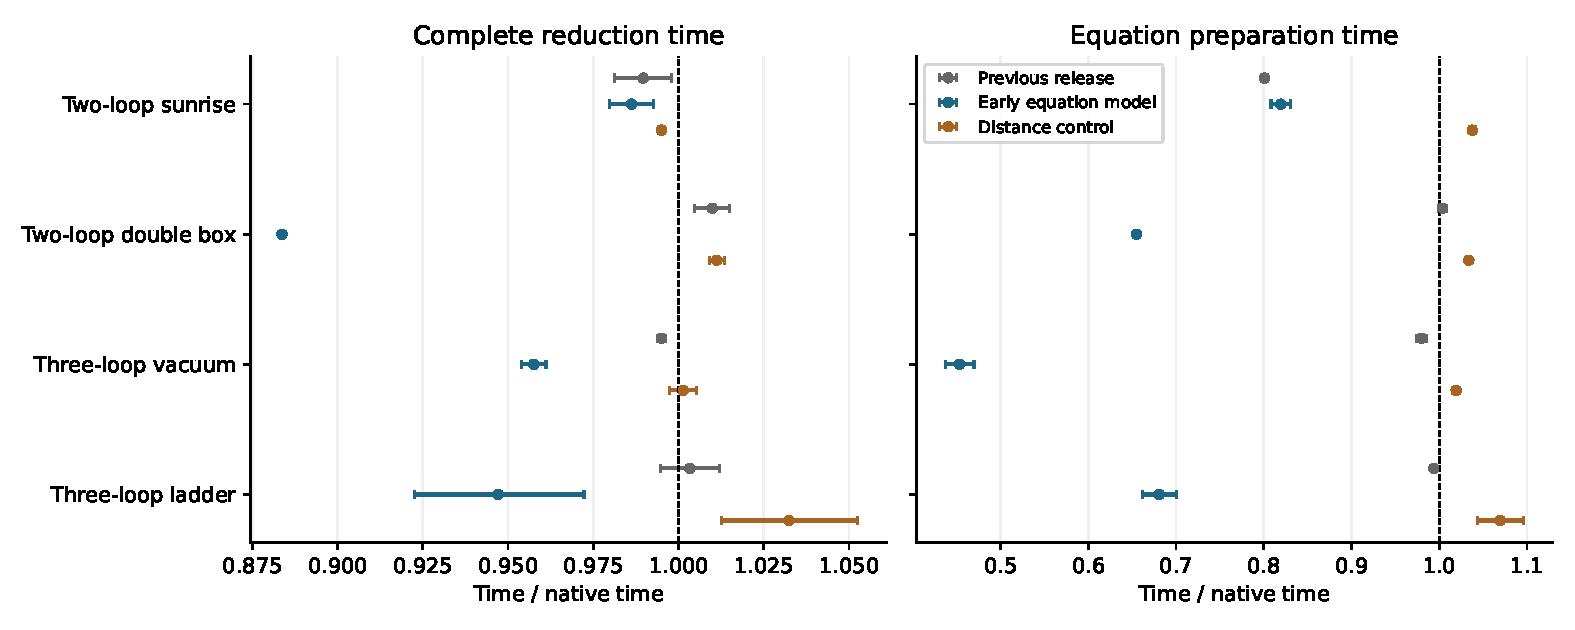
\includegraphics[width=\textwidth]{figures/early_equation_costs.pdf}
 \caption{Complete and equation-preparation time relative to native choices.
 Points use physical-profile weighting and intervals resample profiles.
 Each topology has two new physical profiles.}
 \label{fig:early-equation-costs}
\end{figure}
\begin{figure}[htbp]
 \centering
 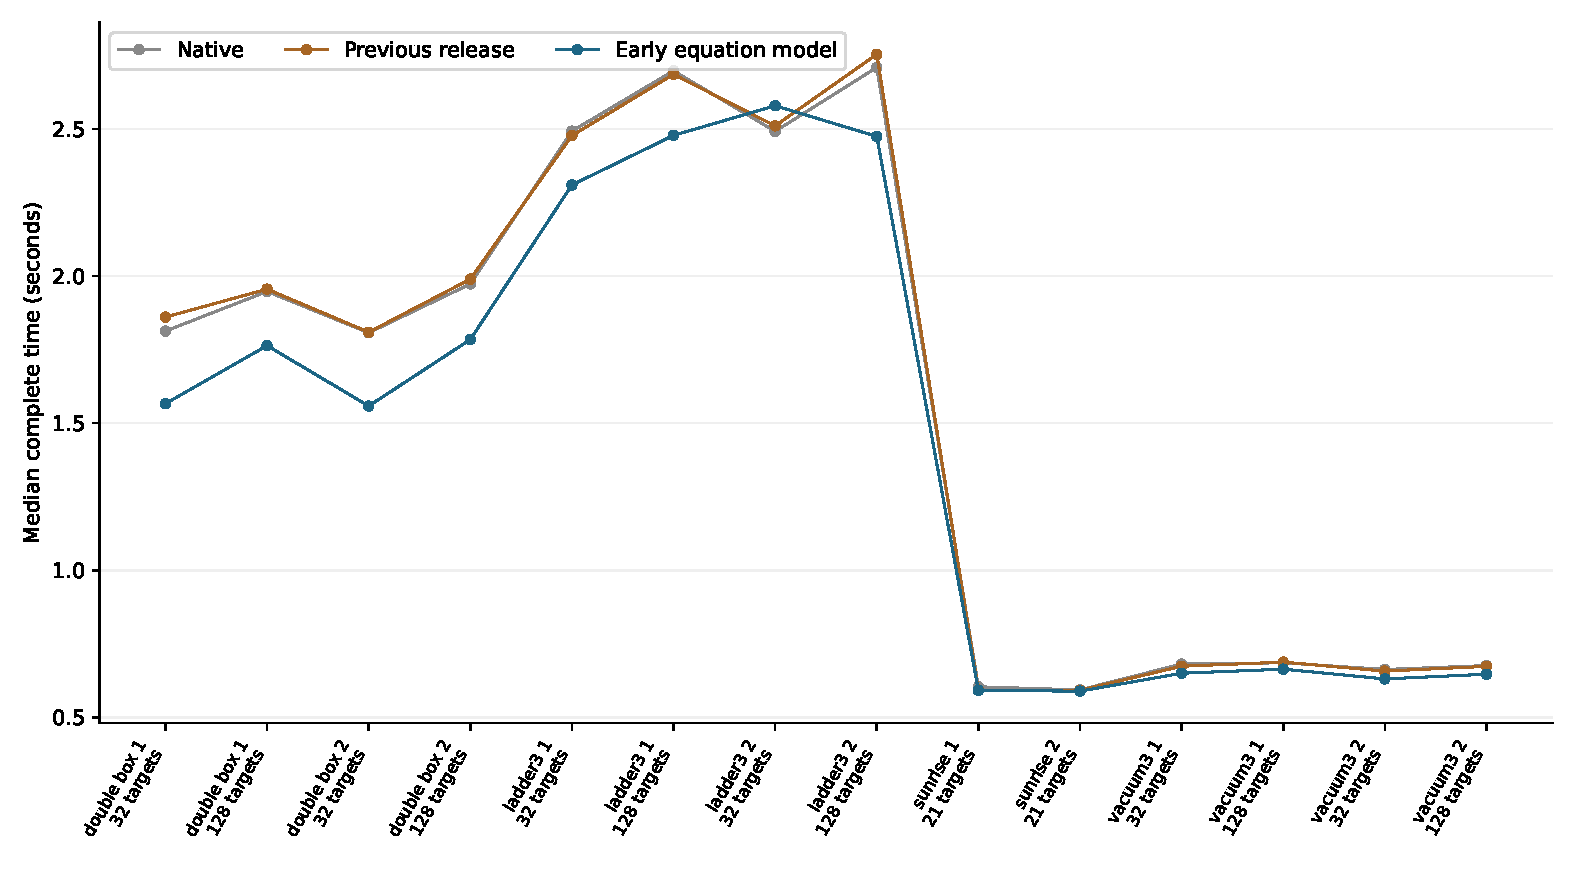
\includegraphics[width=\textwidth]{figures/early_equation_batches.pdf}
 \caption{Median complete time for each fixed target batch, including
 inference, exact checks and all fallback attempts. Each point is the
 median of five alternating repetitions.}
 \label{fig:early-equation-batches}
\end{figure}

All 280 comparison workflows and 8 additional applications pass the independent exact audit. The applications receive only the prescribed basis, and their coefficients agree with the reference after execution. The audit checks 94,970 coefficient pairs, including 1,915 distinct pairs. Every method completes on its first attempt. Maximum sampled memory for Kira and its child processes is 53.46 MiB, and maximum temporary solver storage is 1.39 MiB.

These results test a trained decision before native equation construction,
with complete costs and exact output checks. They establish the measured
domain at fixed rational kinematics. General symbolic multiscale
coefficients, new graph structures, broader target lists and high-loop
reductions require separate evidence. Section~\ref{sec:generalization} supplies subsequent tests on new scattering
structures with independent symbolic invariants. The earlier negative comparisons
remain part of the study, and the selected route activates only the
combinations supported by validation~\cite{KiraEarlyEquationData}.
\FloatBarrier

\subsection{Equation selection and shared reductions at higher loop orders}
\label{sec:higher-loop-acceleration}
The preceding native comparisons cover specific structures with two or three loops. To study the higher orders already present in the integral
collection, we now use the coupled vacuum family in
Eq.~\eqref{eq:coupled-vacuum}. This family has one power of each massless
denominator and two to four distinct massive denominators that depend on
the same momentum \(Q\). Its Euler identities and mass partial fractions
remain valid for any positive integer number of loops. This structure
allows us to test every order from one through twelve with an exact
reference, while keeping the family restriction explicit.

The dependence on the loop order suggests a further reduction in repeated
work. Let \(B=\sum_j b_j\), retain the squared-mass scale \(\mu\), and define
\begin{equation}
 z=L(d-2),\qquad
 W^{(L)}_{\boldsymbol b}=\mu^{B-1}V^{(L)}_{\boldsymbol b}.
 \label{eq:loop-shared-variable}
\end{equation}
The rescaling gives every \(W^{(L)}_{\boldsymbol b}\) the same mass dimension
as the masters \(M_j^{(L)}\). Equations~\eqref{eq:higher-loop-euler} and
\eqref{eq:higher-loop-partial-fraction} then become
\begin{align}
 0&=(z-2B)W^{(L)}_{\boldsymbol b}
       +2\sum_j b_j\rho_j W^{(L)}_{\boldsymbol b+\boldsymbol e_j},
 \label{eq:loop-shared-euler}\\
 0&=(\rho_i-\rho_j)W^{(L)}_{\boldsymbol b}
       -W^{(L)}_{\boldsymbol b-\boldsymbol e_i}
       +W^{(L)}_{\boldsymbol b-\boldsymbol e_j}.
 \label{eq:loop-shared-mass}
\end{align}
Here \(\rho_j\) is the positive squared-mass ratio defined earlier, and the
second identity requires \(b_i,b_j>0\).
The coefficient equations depend on \(L\) only through \(z\). We can
therefore solve one system over \(\mathbb Q(z)\) at fixed rational mass
ratios and obtain
\begin{equation}
 V^{(L)}_{\boldsymbol b}
 =\mu^{1-B}\sum_{j=1}^{R}
 C_{\boldsymbol b j}\bigl(L(d-2);\boldsymbol\rho\bigr)M_j^{(L)}.
 \label{eq:loop-shared-result}
\end{equation}
Each \(C_{\boldsymbol b j}\) is a polynomial in \(z\) with rational
coefficients in the present domain. The master integrals retain their
physical dependence on \(L\). The shared calculation supplies their
reduction coefficients.

We next reduce the number of identities passed to Kira. For a mixed
integral, the model scores each allowed pair \((i,j)\) in
Eq.~\eqref{eq:loop-shared-mass}. The selected identity replaces that integral
with two integrals of total massive power \(B-1\). We repeat the choice for
the resulting integrals and merge repeated dependencies across the target
batch. An integral with only one massive denominator uses
Eq.~\eqref{eq:loop-shared-euler} at the seed
\((k-1)\boldsymbol e_j\) to reduce power \(k\). At \(B=1\), the integral
belongs to the prescribed master basis. This decreasing total power
proves termination and sufficiency for every allowed model choice. Mass
partial fractions carry no IBP seed; the saved dependency choices also
determine the actual Euler seeds with one massive denominator.

The training reference counts the distinct nonmaster integrals in
recursively chosen dependency sets. If \(\mathcal D(\boldsymbol b)\)
denotes such a set, the candidate cost is
\begin{equation}
 c(\boldsymbol b;i,j)=
 \left|\{\boldsymbol b\}\cup
 \mathcal D(\boldsymbol b-\boldsymbol e_i)\cup
 \mathcal D(\boldsymbol b-\boldsymbol e_j)\right|.
 \label{eq:loop-choice-teacher}
\end{equation}
Every pair tied for the smallest candidate cost receives label one.
The recursion fixes a valid local reference and does not establish the
minimum cost for an entire target batch. We train small classification
trees using the ordered massive powers, pair positions, active-denominator
count and simple power summaries. There are 18 features, with no loop order
feature. The absence of \(L\) follows from
Eqs.~\eqref{eq:loop-shared-euler}--\eqref{eq:loop-shared-mass}.
A leaf score is an empirical training frequency. The runtime selects the
highest score and uses exact identities for the algebra. For two active
massive denominators, the single available pair is selected directly.

The training set contains 2,016 candidate actions in
546 exponent shapes, with total power through nine.
We fit depth limits four, eight and twelve using a minimum child size of
four examples. Validation selects the depth-4 candidate, which
contains 15 nodes. On 277 distinct development coefficients, the reader
agrees with symbolic algebra and takes 0.159 seconds,
compared with 4.149 seconds for the symbolic
reader. This reading improvement applies to every comparison arm and is
separate from the learned decision.


Kira solves each selected system through its interface for supplied
systems~\cite{Kira2,Kira3}. We generate the Euler and mass identities
within the measured workflow and use the same native elimination policy
for every comparison arm. This experiment measures supplied-identity
reductions. It does not measure Kira's native generation of a general
IBP system at higher loop orders. The earlier native benchmarks retain that separate
role.

The integration reads the exported coefficients with bounded rational
polynomial arithmetic and checks that polynomial division leaves zero
remainder. Development comparisons against symbolic algebra check this
reader independently. The final check uses the Taylor partial fraction
formula in Eq.~\eqref{eq:higher-loop-reference}, which does not follow the
selected dependency path. The workflow rejects unresolved nonmaster
integrals and retains a fallback to the full equation pool. Timings include input and
model loading, selection, equation construction, Kira, coefficient reading,
substitution, verification and any fallback. We also report external
process times, which include Python startup and evidence writing.
Queue waiting time and offline training are excluded.

The refined validation contains 144 workflows on six batches of mass profiles.
It compares the three trees with first-pair, smallest-pair, largest-pair and
extreme-pair rules and the full pool. Each candidate has three repetitions.
The extreme-pair rule chooses an active denominator with the smallest
power and one with the largest power. Validation selects the
extreme route; the selected learned candidate costs
1.7\% more than the selected rule.
We freeze sources, weights, profiles and target lists before 90 reserved
workflows. The reserved set has two profiles for each of
\(R=2,3,4\), with maximum powers eight and twelve, and runs every
\(L=1,\ldots,12\). Some exponent shapes with lower powers also occur in
training; the cases with maximum power twelve extend its power bound. The tests vary
mass profiles within the same topology and do not test new graph classes.
We use three repetitions and report geometric means of the six ratios of
batch medians. Descriptive intervals resample those six batches.


For each mass profile and target batch, we compare separate reductions with the full equation pool at each \(L\), separate learned reductions, a shared reduction with the full equation pool in \(z\), a shared reduction with a simple rule, and a shared learned
reduction. The full pool contains Euler seeds through the largest target
power and all mass-pair identities through one additional power. The
control with a simple rule uses the rule selected on validation. All arms use the
same project Kira binary with the earlier runtime improvements and native
row choices. These controls separate the benefit of exact loop reuse from
the benefit of selecting a smaller equation set.

For separate reductions at each loop order, learned selection gives
a complete-time ratio of 0.911 to the full pool, with
descriptive interval \([0.815,0.986]\).
With exact loop reuse in both arms, learned selection gives a ratio of
0.925 to the shared full pool, with interval
\([0.889,0.958]\).
The learned/shared ratio to the rule/shared control is
0.968, with interval
\([0.927,1.003]\).
These comparisons keep the incremental learned effect separate from
the exact reuse of coefficient equations.

The deployed shared route gives a complete-time ratio of
0.155 to separate reductions with the full equation pool, with interval
\([0.132,0.184]\).
This corresponds to 6.47 times faster execution of the
twelve-order workload under the stated timing definition.
Figures~\ref{fig:higher-loop-complete-time} and
\ref{fig:higher-loop-equations} show the batch costs and equation counts.
Validation fixes the deployed rule before these tests; we retain the
learned results as a measured alternative.

We separate calculation time from the cost of starting Python and archiving
the test evidence. Before those two outer costs, the separate learned
route has time ratio 0.943, with descriptive interval
\([0.873,0.995]\), to the full pool.
The time spent inside Kira has ratio 0.965, with interval
\([0.925,0.992]\).
Thus the calculation saves 5.7\% and Kira itself saves
3.5\% in this comparison. Archiving fewer source
equations contributes to the larger saving in external process time.

With shared coefficients, the ratio of calculation times of the learned route
to the full pool is 0.966, with interval
\([0.941,0.982]\).
Its ratio to the control with a simple rule is 0.997, with interval
\([0.984,1.011]\).
This comparison does not establish an added advantage over the simple rule.
The deployed shared calculation has ratio 0.128 to separate
calculations with the full equation pool, with interval
\([0.102,0.164]\).
The exact change of variable supplies the main reduction in repeated work.


\begin{figure}[htbp]
 \centering
 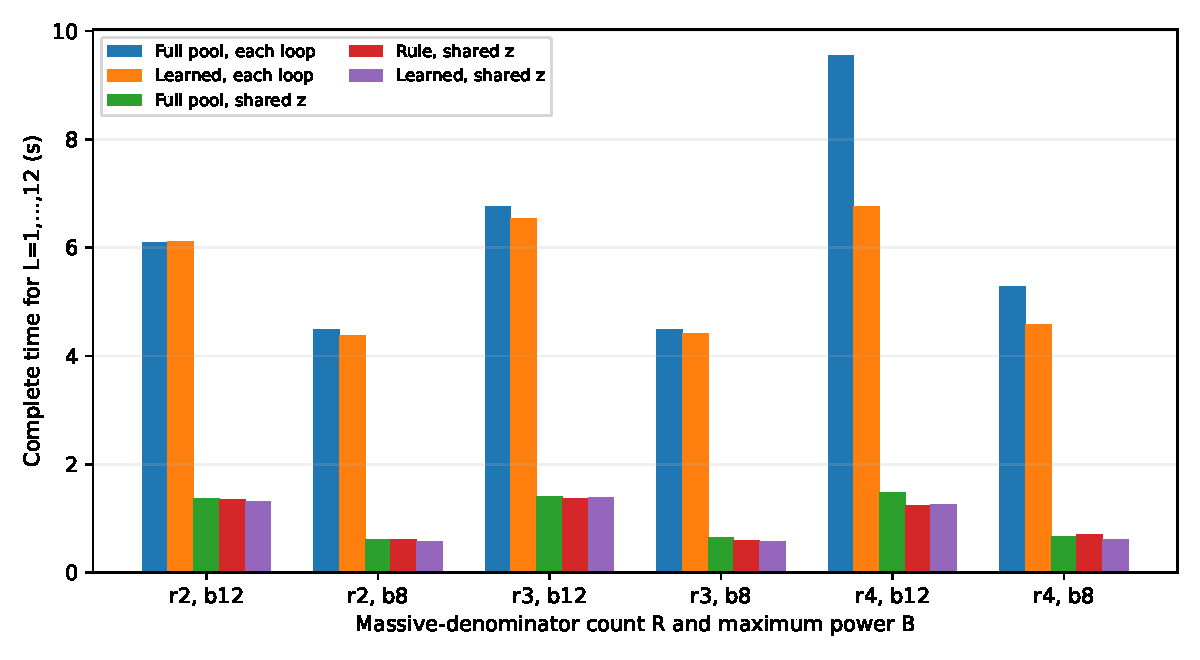
\includegraphics[width=0.98\textwidth]{figures/higher_loop_complete_times.pdf}
 \caption{Median external complete times for the twelve loop orders in
 each reserved batch. Each bar includes the full cost of its stated
 workflow. The shared methods solve once in \(z\) and check the substituted
 coefficients separately at every requested loop order.}
 \label{fig:higher-loop-complete-time}
\end{figure}

\begin{figure}[htbp]
 \centering
 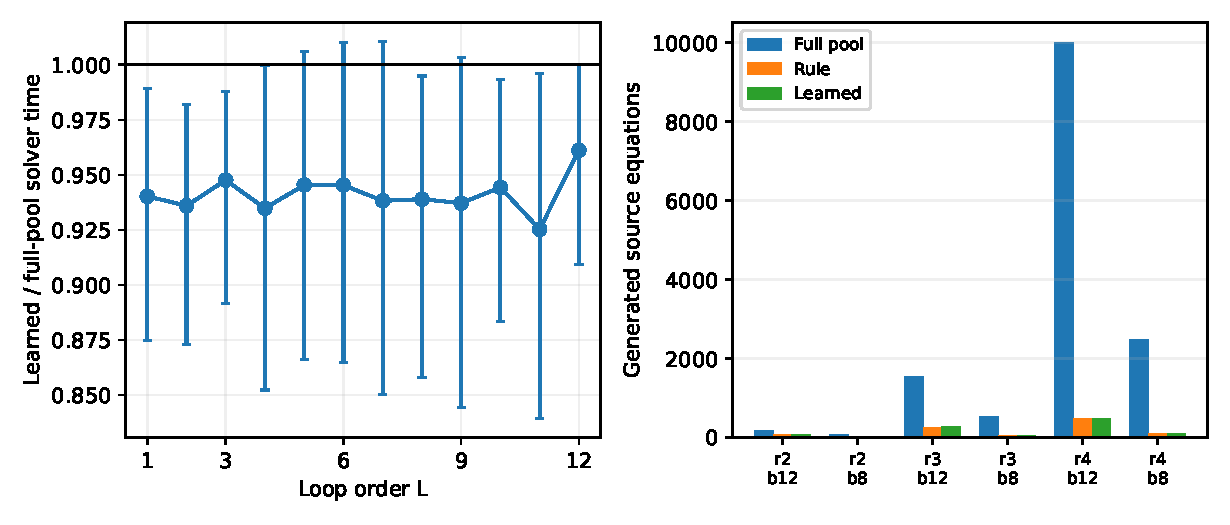
\includegraphics[width=0.98\textwidth]{figures/higher_loop_equations.pdf}
 \caption{Separate-loop solver-time ratios and generated equation counts.
 The left panel includes construction, prediction, Kira and coefficient
 reading for each loop order; the complete workflow also includes the
 checks shown in Fig.~\ref{fig:higher-loop-complete-time}. The intervals
 describe variation across the six reserved batches.}
 \label{fig:higher-loop-equations}
\end{figure}

All 90 reserved workflows and six additional applications pass exact
checks. The extra applications use loop orders 13, 16, 24 and 32.
The audit checks 65,504 coefficient positions, including
5,696 distinct positions, across
492 Kira calls. It finds 0 failed attempts
and 0 fallback workflows.
The largest sampled memory of Kira and its child processes is
23.05 MiB, and the largest temporary
solver storage is 0.58 MiB.
The analytic reference also supplies a direct reduction for this
special family. The reported comparisons measure routes that use Kira.


Equation~\eqref{eq:loop-shared-result} holds for any positive \(L\) in this
scalar family. The finite tests cover the stated orders. Generic scattering
families contain additional scalar products, numerator powers and kinematic
variables, so their native IBP reduction needs separate tests. These results
apply to the stated coupled vacuum family and supplied
identities~\cite{KiraHigherLoopData}.


\subsection{Learning equation choices for groups of targets}
\label{sec:batch-reuse}
The shared variable in Eq.~\eqref{eq:loop-shared-variable} removes repeated
reductions at different loop orders. We now reduce repeated work within
each target set and across independent mass profiles of the same restricted
vacuum family. The calculation still uses one power of every massless
denominator and \(R=2,3,4\) distinct massive denominators. Kira performs
exact elimination on the supplied Euler and partial-fraction identities,
and the retained native IBP-generation interfaces continue to serve their
previously tested two- and three-loop domains.

For a target set \(\mathcal T\), let \(\pi\) specify an ordering of the
\(R\) massive denominators. At each mixed integral, we use the first two
active denominators in this ordering in Eq.~\eqref{eq:loop-shared-mass}.
Every resulting integral has a smaller total power \(B\), and repeated
integrals share the same subsequent reduction. Let
\(\mathcal D_\pi(\mathcal T)\) be the resulting set of distinct nonmaster
integrals. To train a model that favors small shared systems, we assign
the cost
\begin{equation}
 S_\pi(\mathcal T)=
 \sum_{\boldsymbol b\in\mathcal D_\pi(\mathcal T)}
 \left(3\sum_{j=1}^{R}b_j-2\right).
 \label{eq:batch-weighted-cost}
\end{equation}
The weight increases with the number of polynomial coefficients that can
enter a substitution. It provides a training measure of algebraic work;
actual Kira operation counts and the cost of large rational numbers also
depend on its elimination and simplification choices. The smallest
\(S_\pi\) among the \(R!\) mass orderings supplies a restricted reference
for the quality of a choice. More general reduction paths can have
different costs.

We train ensembles of four and sixteen extremely randomized regression
trees~\cite{Geurts2006ExtraTrees} to predict \(\log S_\pi\), then select the
ordering with the smallest predicted value. The 32 inputs describe the
target count, number of massive denominators, total powers, the mean and mean squared power at each
position of \(\pi\), the largest power, the fraction of targets with that
denominator present, and pairwise mean minima and products of powers.
These inputs describe sharing across the entire target set. Each prediction estimates the reduction cost, while exact identities
and Kira determine the reduction coefficients. Two massive denominators admit a single pair, so those
requests bypass inference.

The training set contains 420 target batches and 6,300 candidate orderings,
with total powers up to fourteen and at most 128 targets per batch.
Both ensembles have maximum depth twelve and at least three training
examples per leaf. We compare their complete calculation times with
four simple ordering rules, the earlier learned pair selector, and
enumeration of all fixed orderings. The first validation uses 324
calculations on twelve new mass profiles and selects the four-tree
ensemble as the cheaper learned candidate. Its time ratio to the
fastest simple rule is 1.000, so single-profile deployment
retains that rule. A further 48 validation applications combine three
profiles at a time and give a learned-to-simple time ratio of
0.925, which selects learned ordering for that route.

The selected trees require 7634 nodes in total. We also store their
unchanged thresholds and leaf values in compiled inference routines to
reduce loading and prediction cost. All 12,600 compared candidate scores
agree exactly with the original tree evaluation. For the selected
ensemble, compiled evaluation takes 0.921 times the Python
decision time over the training batches. Fresh complete-calculation
validation then chooses the inference implementation used for production calculations; this comparison includes
model loading and inference and measures the time of the complete calculation.

\subsubsection{Sharing exact checks and Kira calls}
The original shared reduction still expanded and checked the same
coefficient separately at each requested loop order. We instead compare
the Kira coefficient \(C_{\boldsymbol b j}(z)\) with an independent
Taylor partial-fraction construction directly in \(\mathbb Q[z]\).
Exact equality in this polynomial ring implies equality after the
substitution \(z=L(d-2)\) for each requested \(L\). Every returned
coefficient therefore keeps an exact check while each symbolic comparison
takes place once.

We also use integer polynomial arithmetic when reading the coefficients
and applying the substitution. If
\(C(z)=D^{-1}\sum_{n=0}^{q}a_nz^n\), where the \(a_n\) are integers and
\(D\) is a positive common denominator, then the coefficient of \(d^k\)
after substitution is
\begin{equation}
 [d^k]C\bigl(L(d-2)\bigr)
 =\frac{1}{D}\sum_{n=k}^{q}a_n L^n
   \binom{n}{k}(-2)^{n-k}.
 \label{eq:batch-integer-substitution}
\end{equation}
Here \(q\) is the polynomial degree and \([d^k]\) denotes extraction of
the coefficient of \(d^k\). This form keeps the inner sums in integer
arithmetic and reduces the number of repeated fraction normalizations.
These savings follow from exact algebra, separately from the learned
choice of equations.

Independent mass profiles can also share a Kira invocation. We give each
profile its own integral identifiers and master basis, then form
\begin{equation}
 A=\operatorname{diag}(A_1,\ldots,A_P),\qquad
 A\begin{pmatrix}\boldsymbol I_1\\ \vdots\\ \boldsymbol I_P\end{pmatrix}
 =0.
 \label{eq:batch-independent-systems}
\end{equation}
Here \(P\) is the number of profiles, \(A_p\) is the coefficient matrix
of the selected identities for profile \(p\), and \(\boldsymbol I_p\)
contains its integrals. Kira reduces this combined system in one call.
The output checks require each target to contain only masters of its own
profile, after which the same independent symbolic checks apply.
The learned model chooses the equations for each profile before assembly.
The current interface admits up to eight profiles, 512 targets and
12,000 selected equations per call. The timing tests use three profiles
per call. A failed combined reduction retries the profiles separately,
and a failed selected system uses the preserved full supplied system.

\subsubsection{Independent timing and correctness results}
The first reserved comparison uses twelve new mass profiles, powers up to
fourteen, up to 96 requested targets per profile and every loop order
from one through twelve. Five repetitions of five methods give 300
complete calculations. The learned route with shared checks has time
ratio 0.394 to the preceding release, with descriptive interval
\([0.314,0.487]\). Its ratio to the updated simple rule is 0.986,
with interval \([0.955,1.019]\). These measurements separate the common
arithmetic improvements from the additional equation-choice model.
The mean weighted-cost ratio to the best enumerated mass ordering is
1.035. This reference concerns Eq.~\eqref{eq:batch-weighted-cost}
within the finite set of mass orderings.

We then compare separate and combined reductions on four groups of
three of these profiles. Eighty complete applications give a
combined-to-separate learned time ratio of 0.516, with interval
\([0.485,0.563]\). Within combined calculations, the learned-to-simple ratio
is 1.025, with interval \([0.941,1.121]\). This comparison counts
the model cost on both sides where the model is used.

A second reserved set contains twelve further mass profiles, powers up
to thirteen and up to 80 requested targets per profile. Eighty
applications compare the preceding separate workflow, the updated
combined simple rule, and both learned inference implementations on the same
four groups. The compiled learned route has complete-time ratio
0.218 to the preceding workflow, with interval \([0.169,0.276]\), and
ratio 0.923 to the combined simple rule, with interval
\([0.885,0.962]\). Its ratio to Python inference in the otherwise
identical learned workflow is 0.990, with interval
\([0.885,1.117]\). The two learned implementations produce identical selected
equation systems. Complete-time validation retains the Python learned inference implementation for combined requests and the simple rule for a single profile. The compiled inference implementation remains available with its measured comparison.

All 460 reserved applications pass exact checks without fallback.
Separate integration checks cover loop orders 1, 12, 16, 24 and 32 and
include one deliberately failed check that successfully invokes the full
system fallback. The independent audits check 54,594 saved
coefficient occurrences in expanded loop-dependent expressions, and the
final audit also compares 21,675 raw Kira coefficient occurrences
with the earlier rational-expression reader. The peak sampled Kira
process-tree memory is 21.27 MiB and peak native scratch use is
0.75 MiB in these tests.

Complete calculation time includes input reading, model loading,
equation selection and construction, Kira execution, exact coefficient
reading, loop substitution, verification and any fallback. Separate
external-process measurements also include Python startup and evidence
archiving. Reported ratios are geometric means of batch median ratios;
the descriptive 95\% intervals resample the twelve single batches or
four combined groups. The small number of groups limits conclusions
about other workloads. Figure~\ref{fig:batch-reuse-single} shows the
single-profile comparison, and Fig.~\ref{fig:batch-reuse-packed} shows
the second combined comparison~\cite{KiraBatchReuseData}.

These results support acceleration within the stated vacuum family and
fixed mass profiles. The Taylor construction also supplies a direct
analytic solution for this family; these comparisons concern the
reductions performed through Kira here. General scattering families,
native generation of high-loop IBP systems and a globally fastest
reduction remain outside the evidence.

\begin{figure}[htbp]
 \centering
 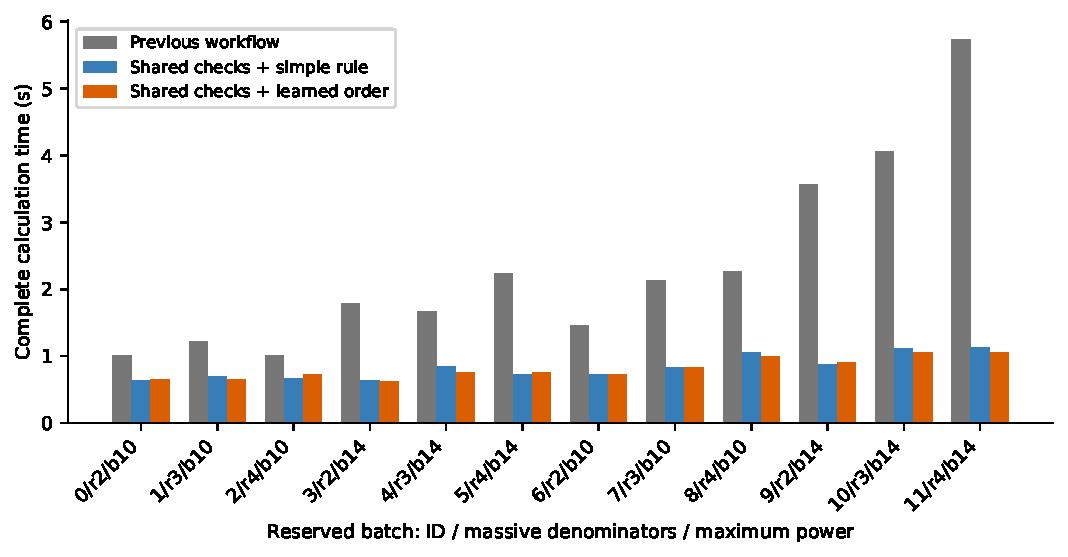
\includegraphics[width=\textwidth]{figures/batch_reuse_single.pdf}
 \caption{Median complete calculation time for the twelve reserved
 single-profile batches. All methods return the same exact reductions
 at loop orders one through twelve. The updated simple and learned
 routes share the improved exact checks and coefficient arithmetic.}
 \label{fig:batch-reuse-single}
\end{figure}
\begin{figure}[htbp]
 \centering
 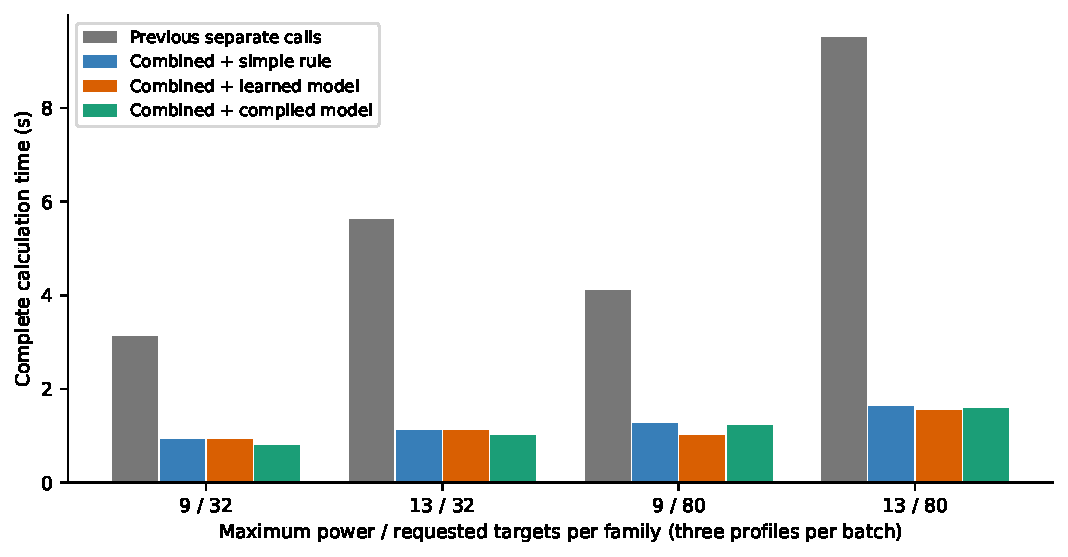
\includegraphics[width=\textwidth]{figures/batch_reuse_packed.pdf}
 \caption{Median complete time for the second reserved comparison.
 Each group contains three independent mass profiles. The previous
 route makes separate Kira calls; the other routes combine the selected
 systems. The target count on the axis is the requested count per
 profile and is capped by the available index vectors.}
 \label{fig:batch-reuse-packed}
\end{figure}


\subsection{Exact pre-reduction and a checked direct path}
\label{sec:pre-reduction}
The combined workflow in Section~\ref{sec:batch-reuse} still spends much
of its time in Kira after the model selects sufficient identities.
For the restricted vacuum family, every selected identity lowers the total
massive-denominator power. We can therefore evaluate the substitutions
in increasing order of that power and return the completed result after
an independent exact check. Kira remains available for comparison and
as a fallback when this direct path fails its checks.

Let \(\boldsymbol C_{\boldsymbol b}(z)\) be the vector of coefficients
of the prescribed masters in \(W_{\boldsymbol b}^{(L)}\), with
\(z=L(d-2)\) as defined earlier. For the master with index
\(\boldsymbol e_j\), this vector is the unit vector
\(\boldsymbol C_{\boldsymbol e_j}=\boldsymbol e_j\).
The selected mass identity gives
\begin{equation}
 \boldsymbol C_{\boldsymbol b}(z)=
 \frac{\boldsymbol C_{\boldsymbol b-\boldsymbol e_i}(z)
       -\boldsymbol C_{\boldsymbol b-\boldsymbol e_j}(z)}
      {\rho_i-\rho_j},
 \qquad b_i,b_j>0.
 \label{eq:pre-mass}
\end{equation}
Here \(\rho_i\) and \(\rho_j\) are the distinct positive mass ratios
specified for the family. When only denominator \(j\) is present,
the Euler identity gives
\begin{equation}
 \boldsymbol C_{k\boldsymbol e_j}(z)
 =\frac{2(k-1)-z}{2(k-1)\rho_j}
   \boldsymbol C_{(k-1)\boldsymbol e_j}(z),
 \qquad k\geq 2.
 \label{eq:pre-euler}
\end{equation}
Both formulas reduce \(B=\sum_j b_j\), so they terminate at the
specified masters. We evaluate each distinct intermediate integral once.

The existing four-tree model selects the mass ordering before these
substitutions, with unchanged weights and training examples.
The learned direct route uses the previously checked compiled evaluator.
We store each polynomial coefficient as integers over a positive common
denominator and cancel their common divisor after each addition or scaling. This keeps the arithmetic exact and reduces
repeated fraction normalization. The model selects the intermediate
integrals that we visit, while Eqs.~\eqref{eq:pre-mass} and
\eqref{eq:pre-euler} determine their coefficients.

An independent Taylor partial-fraction construction checks the result.
For an auxiliary dimensionless variable \(x\), define
\begin{equation}
 \prod_{i:b_i>0}(x+\rho_i)^{-b_i}
 =\sum_{j:b_j>0}\sum_{k=1}^{b_j}\frac{a_{jk}}{(x+\rho_j)^k},
 \qquad
 a_{jk}=[t^{\,b_j-k}]
       \prod_{\substack{i\ne j\\b_i>0}}
       (\rho_i-\rho_j+t)^{-b_i}.
 \label{eq:pre-taylor}
\end{equation}
Here \([t^n]\) means the coefficient of \(t^n\) in the Taylor series.
The corresponding master coefficient is
\begin{equation}
 C_{\boldsymbol b j}(z)=
 \sum_{k=1}^{b_j}a_{jk}
 \prod_{h=1}^{k-1}\frac{2h-z}{2h\rho_j}.
 \label{eq:pre-independent}
\end{equation}
An empty product equals one. This construction uses the same exact
single-denominator relation and obtains the mixed-denominator
coefficients independently of the selected pairs.
We require equality of every polynomial coefficient before substituting
\(z=L(d-2)\). A failed check retries the original request through the
preceding Kira route and its existing full-system fallback.

We compare five routes on identical targets. The preceding deployed route
sends model-selected equations to Kira. A second route first evaluates
the recurrence, then sends the completed target-to-master relations to
Kira. Three direct routes return checked coefficients: one uses learned
ordering, one uses simple extreme-power ordering, and one constructs
the answer with Eq.~\eqref{eq:pre-independent} and checks it with the
simple recurrence. The last route supplies an analytic control that
includes an independent exact check.

Six new three-profile batches provide 90 validation calculations.
Their mass ratios lie outside the ranges used in earlier training and
tests. Validation selects the simple direct route before evaluating eight
further three-profile batches with masses in a separate range.
Each profile has two, three or four massive denominators, the largest
total power is fourteen, and every request includes loop orders one
through twelve. Five repetitions of five routes give 200 reserved
calculations, all of which pass exact checks without fallback.
The independent audit checks 30924 expanded master-coefficient
positions and compares 25770 raw Kira coefficient expressions with the
earlier rational reader. Five further applications include loop orders
1, 12, 16, 24 and 32 and a deliberately failed direct check that recovers
through Kira.

The selected route has calculation-time ratio 0.306 to the preceding
combined learned workflow, with descriptive interval \([0.246,0.373]\).
Its full worker-time ratio is 0.430, with interval \([0.414,0.446]\).
Calculation time includes request reading, model loading and inference
where used, preparation, exact algebra, checks, loop substitution and
fallback. Full worker time also includes interpreter startup and saving
the output. We take the median of five repetitions per batch and then
the geometric mean of the eight batch ratios. The intervals resample
those eight batches and describe this finite comparison.

The learned direct route has calculation-time ratio 0.982
to the simple direct route, with interval \([0.971,0.997]\), and ratio
0.991 to the analytic control, with interval \([0.973,1.013]\).
The comparison does not establish a further complete-time advantage from learned ordering over both direct controls.
Pre-reduction followed by Kira has time ratio 0.927 to the
preceding route. Figure~\ref{fig:pre-reduction-times} shows the batch times.
The principal saving in the direct routes comes from finishing the exact
triangular recurrence before a Kira invocation is needed.
These measurements cover an outer reduction path for the stated vacuum
family. Native IBP-generation policies retain their previously tested
domains, and general high-loop families require separate comparisons.
The implementation, fixed choices, raw outputs and checks accompany the
measurements~\cite{KiraPreReductionData}.

\begin{figure}[htbp]
 \centering
 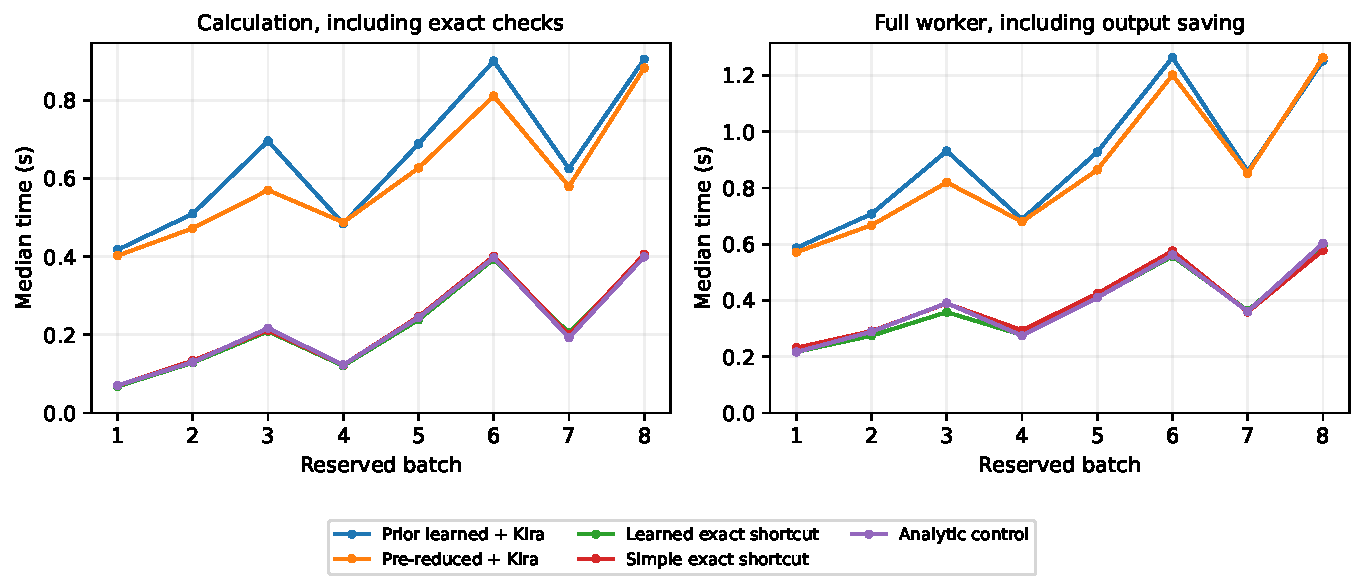
\includegraphics[width=\linewidth]{figures/pre_reduction_times.pdf}
 \caption{Reserved batch times for the preceding Kira route,
 pre-reduction followed by Kira, and three independently checked direct
 routes. Each point is the median of five complete calculations.
 The right panel includes startup and saving the output.}
 \label{fig:pre-reduction-times}
\end{figure}


\subsection{Sharing exact polynomial work across targets and loop orders}
\label{sec:polynomial-reuse}
The direct reduction in Section~\ref{sec:pre-reduction} removes the Kira
call when exact recurrence relations complete the requested reduction.
Its remaining cost includes construction of the independent check and
expansion of each coefficient at every requested loop order. We now reuse
the algebraic terms that these operations have in common and keep the
calculation process available for a bounded sequence of requests.
The master basis, selected identities and exact checks remain the same.

Write a coefficient as
\(C(z)=D^{-1}\sum_{n=0}^{q}a_nz^n\), where \(D\) is a positive integer,
the \(a_n\) are integers, and \(q\) is its degree. For each loop order
\(L\), define the integer transformation
\begin{equation}
 \begin{aligned}
 T^{(L)}_{kn}&=
 \begin{cases}
 \displaystyle\binom{n}{k}L^n(-2)^{n-k},& n\geq k,\\
 0,& n<k.
 \end{cases}
 \\[4pt]
 C\bigl(L(d-2)\bigr)&=\frac{1}{D}
 \sum_{k=0}^{q}\left(\sum_{n=k}^{q}T^{(L)}_{kn}a_n\right)d^k.
 \end{aligned}
 \label{eq:reuse-transform}
\end{equation}
Here \(k\) is the power of \(d\) and \(n\) is the original power of \(z\).
We form this transformation once for each requested \(L\) and reuse it
for all target coefficients. The present power limit gives \(q\leq13\).
We also obtain the common denominator once per symbolic coefficient,
then apply the integer transformations and cancel common factors.
This removes repeated binomial coefficients, powers and denominator
construction while retaining the full expanded result.

The independent check in Eq.~\eqref{eq:pre-taylor} contains repeated
Taylor terms. For a positive denominator power \(\beta\), a nonnegative
series index \(n\), and a nonzero mass difference
\(\Delta=\rho_i-\rho_j\), these terms are
\begin{equation}
 [t^n](\Delta+t)^{-\beta}
 =(-1)^n\binom{\beta+n-1}{n}\Delta^{-(\beta+n)}.
 \label{eq:reuse-taylor}
\end{equation}
We retain each required truncated factor within its mass profile and
multiply the factors with integer polynomials over common denominators.
We also form each single-denominator polynomial
\(\prod_{h=1}^{k-1}(2h-z)/(2h\rho_j)\) once for that profile and reuse it
in Eq.~\eqref{eq:pre-independent}. Every target still receives its own
independent master expansion and exact comparison with the selected
recurrence. This reuse changes the arithmetic work needed to construct
the check.

For a sequence of requests, one running process retains the transformation
matrices and, when requested, the unchanged trained model.
Each new mass profile receives fresh mass-dependent Taylor terms, so
a repeated integral identifier cannot transfer coefficients between
different physical inputs. The current interface bounds the retained
transforms and the number of requests per process. A failed exact
comparison retries the preserved Kira route. The previous ordering
policy remains the default, and this extension introduces no new model
training.

We compare the preceding arithmetic, shared transformations alone,
shared Taylor terms alone, and both changes together.
All routes use the same output writer, which stores each exact coefficient
block once. Four new three-profile batches provide 48 validation
calculations and select both arithmetic changes before the reserved test.
Eight further batches provide 160 calculations: four variants with five
repetitions each. The tests use two, three or four massive denominators,
total massive-denominator power \(B\leq14\), up to 96 requested targets
per profile, and every
loop order from one through twelve. Validation and reserved mass ranges
are disjoint from each other and from earlier training and comparisons.

The two changes together have calculation-time ratio 0.372 to the
preceding arithmetic, with descriptive 95\% interval \([0.343,0.402]\).
The ratio including process startup and output saving is 0.682,
with interval \([0.592,0.797]\). Shared transformations alone have
calculation-time ratio 0.701, and shared Taylor terms alone have
ratio 0.693. The combined route reduces expansion time to
0.414 of its previous value and construction time for the
independent check to 0.158.
These ratios compare batch medians and then take the geometric mean over
eight batches. The descriptive intervals resample those eight batches.
Figure~\ref{fig:polynomial-reuse-times} separates the component changes.

We then compare separate processes with one persistent process for streams
of four, four and eight batches. The eight-batch stream contains the
inputs from both four-batch streams. Three repetitions of four
configurations give 36 stream runs and 192 additional batch calculations.
All stream times include initial process startup, input reading,
calculation, exact checks and output saving.
With the updated arithmetic, process reuse has time ratio 0.524
to separate updated processes. Combining arithmetic and process reuse
has ratio 0.365 to separate processes with the preceding arithmetic.
The three specified streams overlap, so we report these descriptive
ratios without a statistical interval.
Figure~\ref{fig:polynomial-reuse-streams} gives the individual stream times.

All 352 reserved batch calculations return identical exact coefficients
across the applicable routes. The independent audit checks 28860
expanded coefficient positions with the older formula at each loop order.
Additional interface checks cover changed masses and loop orders under
the same integral identifier, continued operation after an invalid request,
the request limit, retained model evaluation, and recovery through Kira
after a deliberately failed check. These savings come from shared exact
arithmetic and reduced process startup. They apply to the restricted
vacuum family and its existing reduction interface; the earlier native
IBP-generation scope remains unchanged. The frozen implementation,
measurements and checks are available with the data~\cite{KiraPolynomialReuseData}.

\begin{figure}[htbp]
 \centering
 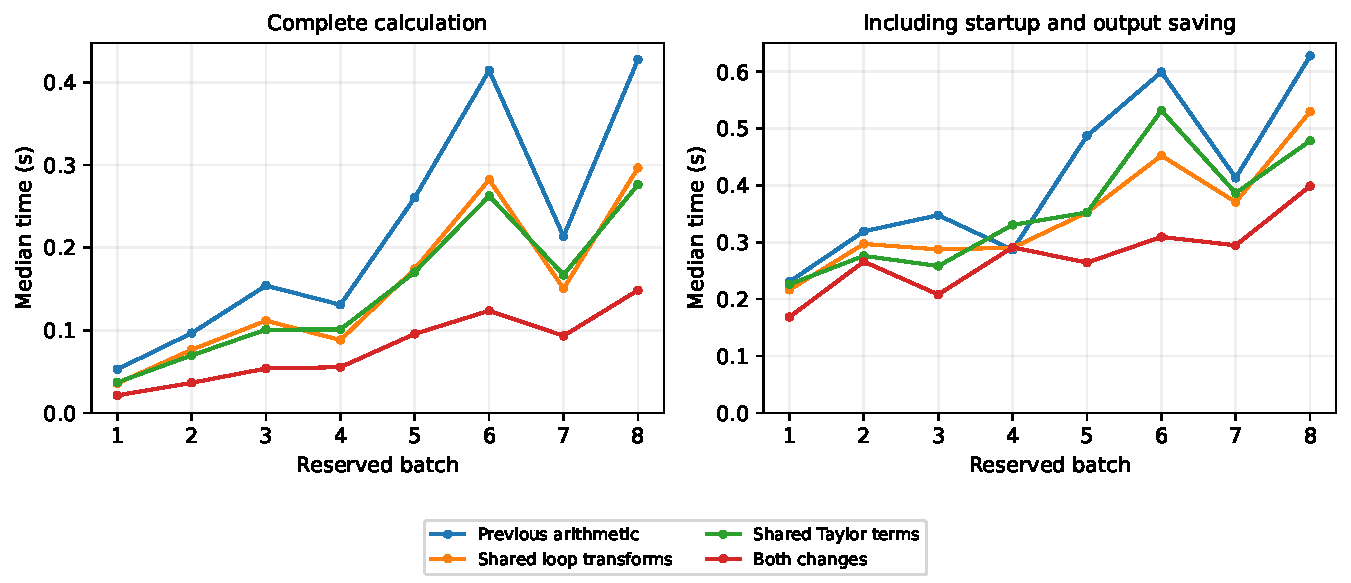
\includegraphics[width=\linewidth]{figures/polynomial_reuse_times.pdf}
 \caption{Reserved batch medians for the preceding arithmetic, each
 reuse change separately, and both changes together. Each point uses
 five complete calculations with identical target outputs and checks.}
 \label{fig:polynomial-reuse-times}
\end{figure}
\begin{figure}[htbp]
 \centering
 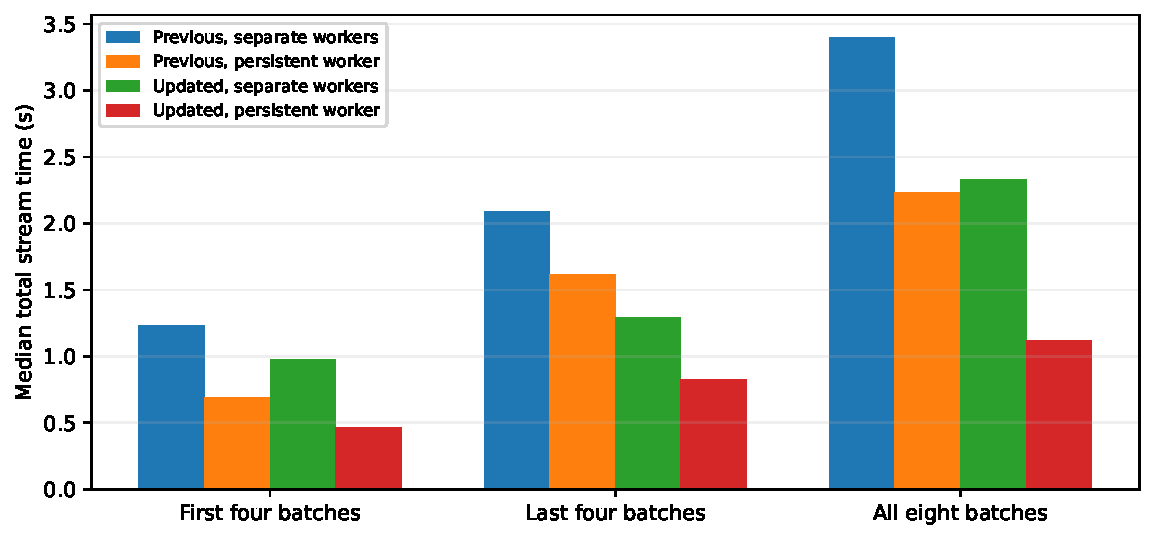
\includegraphics[width=\linewidth]{figures/polynomial_reuse_streams.pdf}
 \caption{Total time for the specified request streams, including startup,
 all exact checks and saving the results. Each bar gives the median of
 three runs. The eight-batch stream uses all inputs from the two
 four-batch streams.}
 \label{fig:polynomial-reuse-streams}
\end{figure}


\clearpage
\subsection{Exact integer arithmetic and learned batch strategies}
\label{sec:exact-backend}
Section~\ref{sec:polynomial-reuse} reuses the transformations for
\(z=L(d-2)\), but its implementation still converts coefficients between
integer polynomials and separate rational numbers. It also writes each
integer as decimal text. We now retain the common-denominator representation,
compile the loop-order expansion, and test a compact exact output format.
We then train a small model to choose a recurrence strategy for a whole
target batch and compare its cost with fixed strategies.

For a polynomial \(C(z)=D^{-1}\sum_{n=0}^{q}u_nz^n\), we store the integer
vector \((u_0,\ldots,u_q)\) and positive denominator \(D\), with
\(\gcd(D,u_0,\ldots,u_q)=1\). Both the selected recurrence and the independent
Taylor construction return this form, so their exact comparison needs
no conversion to separate fractions. The compiled expansion uses
Eq.~\eqref{eq:reuse-transform} to obtain
\begin{equation}
 v_k=\sum_{n=k}^{q}T^{(L)}_{kn}u_n,\qquad
 g_k=\gcd(|v_k|,D),\qquad
 [d^k]C\bigl(L(d-2)\bigr)=\frac{v_k/g_k}{D/g_k}.
 \label{eq:backend-integer}
\end{equation}
Here \(v_k\) is the integer numerator before cancellation, \(g_k\) is its
greatest common divisor with \(D\), and \([d^k]\) extracts the coefficient
of \(d^k\). The implementation uses integer operations from the GNU Multiple Precision
Arithmetic Library (GMP); the installed
library version is 6.0.0~\cite{GMPIntegerManual}. Every coefficient
retains its exact reduced numerator and denominator.

The compact format records the sign, byte length and base-256 digits of
each integer, together with the target, master and loop-order indices.
It therefore preserves the full symbolic and expanded coefficients.
A supplied reader recovers the same coefficient arrays as the decimal
format. We measure the cost of reading these arrays as well as the
cost of producing and saving them, so the comparison includes the
conversion needed by a consumer of the result. The same master basis,
independent Taylor check and Kira fallback apply throughout.

The learned strategy selects one of five rules for each batch.
The first rule is the preceding extreme-power rule. Two further rules
order denominator slots by their total powers across the targets,
in increasing or decreasing order. Another rule selects the active
mass pair with the largest absolute mass difference, and the last
uses a fixed slot order. Each rule generates a terminating set of
exact recurrence relations. The model can change which intermediate
integrals occur and the sizes of the rational coefficients during
substitution.

For batch \(\mathcal B\) and rule \(s\), let \(T_{\mathcal B s r}\) be the
measured time in repetition \(r\) of an already running worker.
This time includes request reading, recurrence selection, exact
arithmetic, the independent check and output writing. The training
target and the rule selected by the model are
\begin{equation}
 y_{\mathcal B s}=
 \log\!\left(\operatorname{median}_{r=1,2,3}T_{\mathcal B s r}\right),
 \qquad
 \widehat s(\mathcal B)=
 \mathop{\operatorname{arg\,min}}_s f_s(x_{\mathcal B}),
 \label{eq:backend-policy}
\end{equation}
where \(x_{\mathcal B}\) contains 49 input features and \(f_s\)
is the tree prediction of the log time for rule \(s\).
The features describe target powers, numbers of active denominators,
loop orders, masses, mass differences, and shared integrals obtained by
lowering one positive target power. We combine profile means and maxima
into a fixed-length batch description. A multi-output regression tree
with maximum depth four and at least six training batches per leaf learns
these costs; the fitted tree has 19 nodes.
The scores estimate runtime and carry no calibrated probability claim.

Training uses 96 batches and 1,440 timed calculations. The first twelve validation
batches provide 324 calculations that compare the preceding
arithmetic, retained integer polynomials, compiled expansion with decimal
output, compiled expansion with binary output, and the learned rule.
The validation also compares every fixed recurrence rule with the compiled
binary route. Each batch contains three profiles with two, three and four
massive denominators. Total massive powers reach fourteen, requested
target counts reach 96 per profile, and every profile includes loop orders
one through twelve. The training, validation and reserved test stages
use distinct targets and mass profiles.

The first validation selects retained integer polynomials with decimal
output. Its reserved comparison contains 504 batch calculations and
passes every exact check. Its full-time ratio, including output reading,
is 0.998 with descriptive interval \([0.867,1.162]\), so this comparison
does not establish a complete-time improvement. The binary variants
reduce production time, but their Python reader adds enough cost to
remove the gain in the full comparison.

We therefore compile the expanded-coefficient reader while retaining the
same binary format, exact arithmetic and trained tree. This change follows
the reader cost observed during validation. The original frozen comparison
remains intact. The compiled reader passes 1,000 loop-output comparisons
with the Python reader and rejects 250 truncated records. A new set of
twelve validation batches supplies 324 further calculations, and a separate
set of twelve test batches supplies the final reserved comparison.
An incomplete reader comparison is excluded because its selection step
referenced the earlier validation set. We preserve those 360 measurements,
correct the stage references, and freeze the prescribed choice from the
new validation set before generating results for fresh reserved targets.

The second validation selects compiled expansion and binary output with a fixed recurrence rule using total process time plus
output reading. A learned route must improve on the best fixed route by at least
two percent to replace it. We freeze the implementation, tree, deployment
choice and test inputs before the reserved comparison.
Twelve new batches then provide 300 separate-process calculations,
with five repetitions per method. The implementation comparison uses
the same request interface and output writer for matched routes.

The selected route has calculation-time ratio 0.522 to the preceding
arithmetic. Its full process-time ratio is 0.850, with descriptive
95\% interval \([0.785,0.909]\), and the ratio including output reading is
0.858, with interval \([0.800,0.914]\).
Retaining integer polynomials alone gives a ratio of 0.981 when
output reading is included. Compiled expansion with decimal output gives
0.933, and compiled expansion with binary output and the preceding
rule gives 0.858. These comparisons separate arithmetic changes
from the output format. The ratios use geometric means of within-batch
median ratios; the descriptive intervals resample the twelve batches.
Figure~\ref{fig:exact-backend-times} shows their measured times.

The learned route has total-time ratio 0.873 to the preceding
arithmetic and ratio 1.017 to the fixed rule selected by validation,
both including output reading. The latter interval is \([0.969,1.070]\).
This interval includes one, so the reserved comparison does not establish a further time reduction from learned choices. The deployed default uses the fixed validation choice.
The model and its measurements remain available with the fixed-rule
controls, including any extra inference cost.

We also compare persistent workers on three disjoint streams of four
reserved batches. Four recorded route labels and three repetitions give 36 stream runs
containing 144 additional batch calculations. The selected route has
stream-time ratio 0.702 to the preceding arithmetic, or
0.725 when reading every output is included.
Figure~\ref{fig:exact-backend-streams} separates these two costs.
The compiled fixed-rule and deployed labels use the same settings and
provide separately timed repetitions. These stream ratios describe the
three specified sequences.
A separate comparison of identical binary blocks gives compiled-to-Python
reader-time ratio 0.147, using five repetitions per reader and batch.

All 444 final reserved batch calculations pass exact comparisons,
and the two comparisons together contain 948 such calculations.
The independent audit checks 35472 expanded master-coefficient
positions against the older loop-dependent formula and verifies equality
between the two output formats. The compiled arithmetic also passes
3,277 earlier exact checks. Additional interface checks cover changed
physical inputs under a repeated identifier, invalid requests, the worker
request limit, truncated output, and recovery through Kira after a
deliberately failed independent check. These results apply to the
restricted coupled vacuum family. The earlier native IBP-generation
results retain their stated domains. The implementation, new tree,
frozen inputs and measurements accompany the report~\cite{KiraExactBackendData}.

\begin{figure}[htbp]
 \centering
 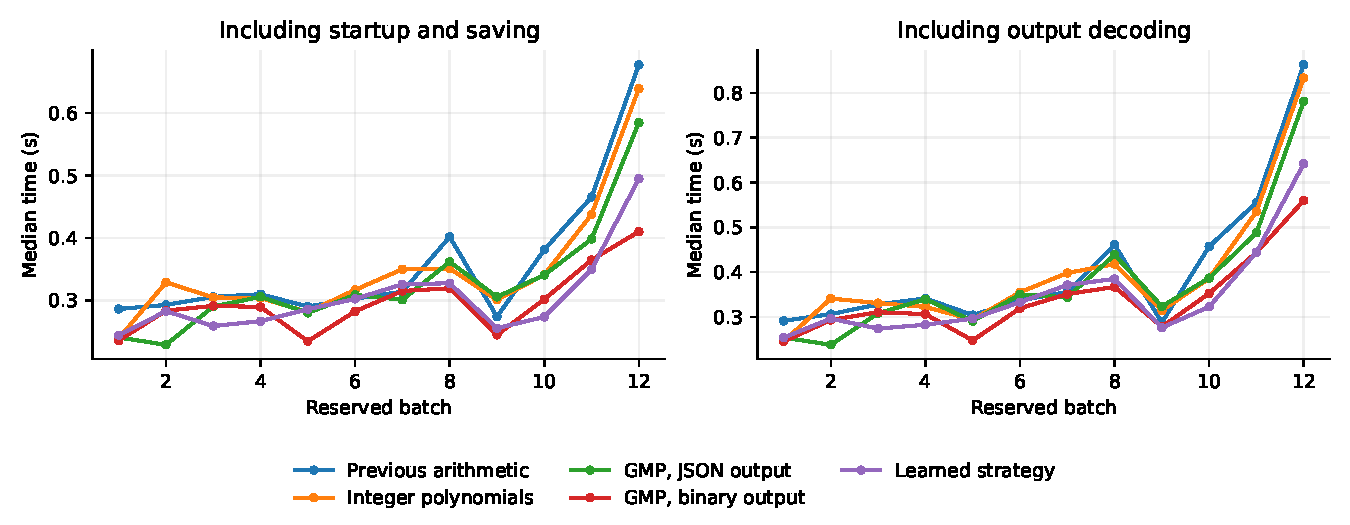
\includegraphics[width=\linewidth]{figures/exact_backend_reader_times.pdf}
 \caption{Reserved batch medians for the arithmetic and strategy variants.
 Each point uses five repetitions. The right panel includes reading and
 decoding the complete exact coefficient output.}
 \label{fig:exact-backend-times}
\end{figure}
\begin{figure}[htbp]
 \centering
 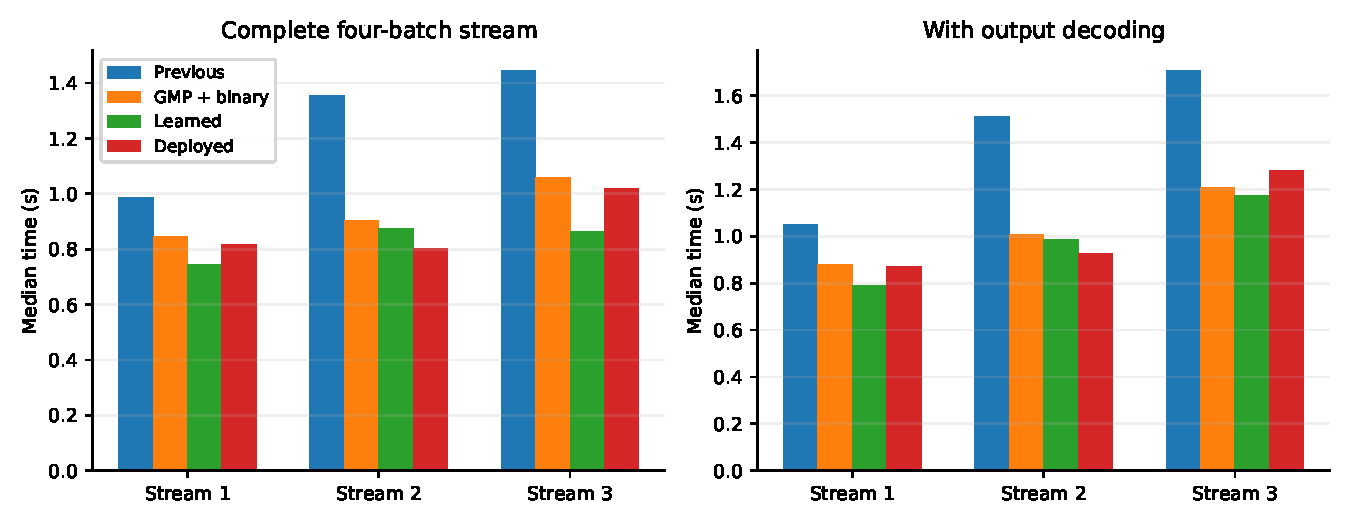
\includegraphics[width=\linewidth]{figures/exact_backend_reader_streams.pdf}
 \caption{Complete times for three disjoint four-batch streams. Each bar
 is the median of three repetitions. The right panel adds reading and
 decoding every output. The deployed route follows the validation choice.}
 \label{fig:exact-backend-streams}
\end{figure}


\clearpage
\subsection{Direct measurement of the cumulative change}
\label{sec:cumulative-speedup}
The preceding sections compare successive changes on different target sets.
To measure the cumulative change directly, we now run the original baseline
and final deployed calculation on identical integrals. We retain the
coupled vacuum family of Eq.~\eqref{eq:coupled-vacuum}, with unit massless
powers, two to four distinct massive denominators and fixed positive
integer mass ratios. We set the common squared-mass scale to \(\mu=1\),
as in the preceding comparisons. Each target has the same prescribed master basis
in every comparison.

The first control uses the saved original Kira 3.1 executable, whose file
hash agrees with the first frozen cost comparison. It generates the full
Euler and mass partial-fraction equation pool and reduces each mass
profile separately at every requested loop order. The Euler seeds extend
through the largest target power, and the mass-pair identities extend
through one additional power. A second control uses exactly the same
requests, equation generation, reader and verification, with the later
project executable used in Section~\ref{sec:higher-loop-acceleration}.
Its learned policies are disabled. Comparing these controls separates
the executable change from the subsequent removal of repeated reductions.

The final route remains the validation-selected implementation from
Section~\ref{sec:exact-backend}. It evaluates the selected recurrences directly and calls Kira only if
the exact check fails. It uses the fixed extreme-power recurrence,
shares coefficients in \(z=L(d-2)\), checks them through the independent
Taylor construction, expands them with compiled exact arithmetic and
saves lossless binary output. It retains the existing Kira fallback.
No model is retrained and no strategy is selected from the cumulative
test results. These calculations use explicitly supplied identities;
the test does not invoke native generation of a general multiloop IBP
system.

We declare eight new groups of three mass profiles, one each with
\(R=2,3,4\), and request every loop order \(L=1,\ldots,12\).
Two groups use each maximum total massive power \(8,10,12,14\).
The requested target counts per profile are \(16,32,48,64\), respectively,
capped by the available index vectors. The mass profiles are new, while
index shapes can overlap earlier data within this restricted family.
A separate upper-bound pilot checks executable compatibility and
resource use. We then freeze the implementations, executable hashes,
final deployment choice and all reserved requests.

Five repetitions of each method give 120 complete workflows.
Both controls use the same scheduler-provided job-local scratch.
Four allocated CPU slots process independent groups on one scheduled
node. Each worker binds to a distinct available physical core, and
every matched comparison remains bound to that core,
with a shuffled sequential order within each three-method block. Each trial starts a fresh
worker process and uses ordinary filesystem caching. Content-addressed
storage can reuse an identical saved output on a repeated trial in any
arm, while each arm recomputes its reduction. The primary time includes
process startup, input loading, equation construction, exact algebra,
verification, output saving, and reading and decoding the full output.
It also includes the diagnostic evidence written inside each worker.
Queue waiting, offline training and the later independent audit lie
outside this time. We separately retain calculation times before
final output saving and reading.

Let \(T_{abr}\) denote the primary time for method \(a\), batch \(b\)
and repetition \(r\). We compare the medians within each batch and
combine the eight ratios through
\begin{equation}
 \widetilde T_{ab}=\operatorname{median}_{r=1,\ldots,5}T_{abr},
 \qquad
 R_T=\exp\!\left[\frac{1}{8}\sum_{b=1}^{8}
 \log\frac{\widetilde T_{\mathrm{final},b}}
               {\widetilde T_{\mathrm{original},b}}\right],
 \qquad
 S=\frac{1}{R_T}.
 \label{eq:cumulative-ratio}
\end{equation}
Here \(R_T\) is the final-to-original time ratio and \(S\) is the cumulative
speedup. The percentage of time saved is \(100(1-R_T)\).
A descriptive 95\% interval resamples the eight complete batches
10,000 times, keeping all repetitions and methods within each batch.
This direct comparison uses neither products of earlier ratios nor
different input sets for the two methods.

The measured time ratio is 0.001839, with descriptive interval
\([0.001653,0.002049]\). It corresponds to 543.815 times faster execution,
with interval \([488.134,605.064]\), and 99.82\% less time.
The ratio to the later full-pool control is 0.012,
corresponding to 81.170 times faster execution.
The calculation subtotal excludes outer worker startup and final output
saving and reading, while retaining every Kira startup within the
baseline reduction. Its final-to-original ratio is 0.000294,
or 3402.846 times faster.
Summing one primary-time median per batch gives 1027.781 seconds
for the original control and 1.922 seconds for the final route,
a workload speedup of 534.881. This sum weights large batches
by their elapsed time, whereas Eq.~\eqref{eq:cumulative-ratio} gives
equal weight to each batch. Figure~\ref{fig:cumulative-speedup} shows
the absolute times and individual speedups.

Within each batch, every method and repetition returns the same exact
expanded coefficients. All 120 reserved workflows complete with no
failure or fallback. Each baseline arm makes 1,440 Kira calls;
the final arm makes none on these successful requests. The independent
audit checks 27960 nonzero target--master coefficient polynomials
after substituting each loop order, using the earlier loop-dependent
Taylor formula. It also regenerates all
288 distinct baseline systems, checks their input hashes and
uses SymPy to read 1464 coefficient positions directly from
saved Kira exports. The two baseline executables receive identical
systems at each mass profile and loop order. The maximum sampled
worker process-tree memory is 78.488 MiB and temporary solver storage
is 1.238 MiB.

The cumulative saving includes shared symbolic reductions, direct
checked recurrences, compiled expansion and reduced output costs.
The fixed-rule deployment makes this a measurement of the complete
mathematical and implementation change. It supplies no separate
ML-only speedup estimate. General scattering families and native
generation of broader high-loop IBP systems remain outside this
comparison. The frozen inputs, implementations, individual timings,
raw exports and audits accompany the report~\cite{KiraCumulativeData}.

\begin{figure}[htbp]
 \centering
 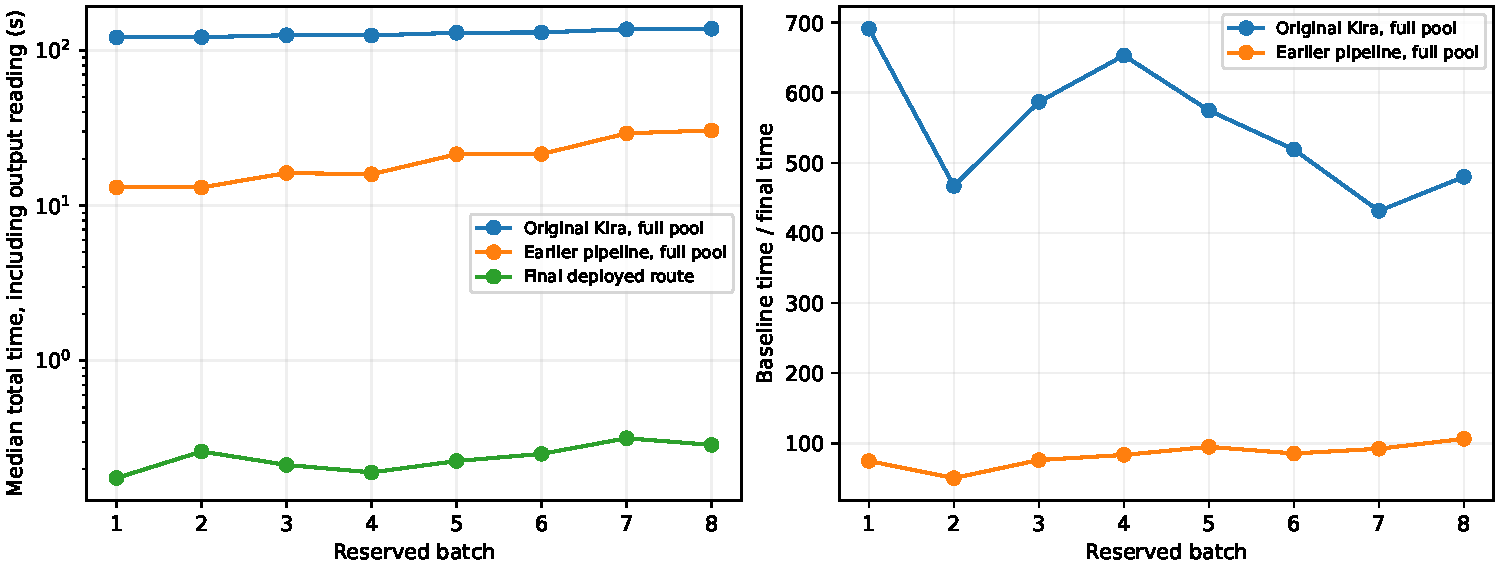
\includegraphics[width=\textwidth]{figures/cumulative_speedup.pdf}
 \caption{Direct cumulative comparison on identical reserved vacuum
 batches. The left panel shows median total times, including output
 reading, on a logarithmic scale. The right panel divides each
 baseline median by the final-route median. Each point uses five
 repetitions, three mass profiles and loop orders one through twelve.}
 \label{fig:cumulative-speedup}
\end{figure}



\clearpage
\section{Scattering families, symbolic kinematics and certified reduction paths}
\label{sec:generalization}
The preceding comparisons establish costs for specified native families and
for a restricted vacuum construction. To extend the physical scope, we now
reduce new four-point and five-point families and retain independent
kinematic invariants as symbols. We also construct small IBP systems for
which every allowed elimination path can be examined. These two extensions
test different questions: whether a frozen learned filter transfers to
new physical inputs, and whether a recorded reduction cost can be proved
minimal within an explicit set of operations.

\subsection{New physical families and independent invariants}
We continue to use $I_{\boldsymbol a}$ for an indexed integral and
$D_i=q_i^2+\mathrm{i}0$ for each massless denominator. The new two-loop
family is the massless limit of the nonplanar four-point family
\texttt{topo4} in Ref.~\cite{KiraOriginal}. Its ordered denominator momenta are
\begin{align}
 \boldsymbol q_{\mathrm{NP}}={}&
 (\ell_1,\ell_2,p_1-\ell_1,p_2-\ell_2,
 p_1+p_2-p_3-\ell_1,\nonumber\\
 &p_1-\ell_1+\ell_2,p_1-p_3-\ell_1+\ell_2,
 \ell_1-p_3,\ell_2-p_1-p_2).
 \label{eq:general-np-momenta}
\end{align}
The first seven entries are physical propagators, and the last two
complete the scalar-product basis and can appear as numerators.
The momenta satisfy $p_1^2=p_2^2=p_3^2=0$ and
$q=p_1+p_2-p_3$ with $q^2=0$. We define
\begin{equation}
 s=(p_1+p_2)^2,\qquad t=(p_1-p_3)^2,
 \qquad
 2p_1\!\cdot p_2=s,\quad
 2p_1\!\cdot p_3=-t,\quad
 2p_2\!\cdot p_3=s+t.
\end{equation}
The symbolic reduction therefore takes place in $\mathbb Q(d,s,t)$.

The new one-loop pentagon has five massless external momenta satisfying
$\sum_{i=1}^{5}p_i=0$. Its denominator momenta are
\begin{equation}
 \boldsymbol q_{\mathrm{P}}=
 (\ell,\ell-p_1,\ell-p_1-p_2,
 \ell-p_1-p_2-p_3,\ell-p_1-p_2-p_3-p_4).
 \label{eq:general-pentagon}
\end{equation}
All five entries are physical propagators. We retain the five adjacent
invariants
\[
 s_{12}=(p_1+p_2)^2,\quad s_{23}=(p_2+p_3)^2,\quad
 s_{34}=(p_3+p_4)^2,\quad s_{45}=(p_4+p_5)^2,\quad
 s_{51}=(p_5+p_1)^2.
\]
Momentum conservation fixes the other scalar products. For example,
$2p_1\cdot p_3=s_{45}-s_{12}-s_{23}$ and
$2p_1\cdot p_4=s_{23}-s_{45}-s_{51}$.
The coefficient field is
$\mathbb Q(d,s_{12},s_{23},s_{34},s_{45},s_{51})$.

A one-loop box supplies an additional test with an external virtuality.
Its denominator momenta are
$(\ell,\ell-p_1,\ell-p_1-p_2,\ell-p_3)$.
Here $p_1,p_2,p_3$ are massless, while
$v=q^2=(p_1+p_2-p_3)^2$ is an independent symbol.
The definitions of $s$ and $t$ remain the same, and
$2p_2\cdot p_3=s+t-v$. Thus its coefficients belong to
$\mathbb Q(d,s,t,v)$. This family has massless internal lines and one
external line with nonzero virtuality.

The denominator coefficient matrices have ranks nine, five and four
for the nonplanar box, pentagon and one-loop box, respectively.
Each rank equals $L(L+1)/2+LE$, where $E$ is the number of independent
external momenta. The external Gram determinants are nonzero as
rational functions and at the specified numerical points.
The calculations use generic kinematics away from singular denominators.
They retain every listed independent invariant, with no replacement
of a scale by one. Internal masses remain zero in these scattering tests.

We first test two rational profiles of the nonplanar box and two of the
pentagon, keeping $d$ symbolic. The box profiles are
$(s,t)=(-149,-147)$ and $(-167,-157)$ in a common squared-momentum unit.
The pentagon profiles are
$(-51,-53,-57,-59,-63)$ and $(-71,-73,-77,-79,-83)$ in the displayed
invariant order. We then test one fully symbolic instance of each of
the three families. Targets start with the full-sector corner and
each single additional propagator power, followed by auxiliary
numerators and singly pinched sectors in a fixed index order.
The four rational-profile batches contain sixteen targets each.
The symbolic nonplanar box, pentagon and one-loop box contain ten,
six and eight targets. The seven batches therefore contain 88 targets.
Their definitions and target lists precede the timed comparisons.

\subsection{Frozen model transfer and exact comparison}
The experiment retains the preceding depth-twelve equation-selection
tree, its weights and its retention threshold $0.01$.
The tree sees seed, operator and target features before Kira constructs
an identity. These scattering topologies were absent from its training
collection. No new fit or threshold selection uses the new results.
Small feasibility pilots establish that the symbolic inputs run
within the resource limits. Some symbolic pilot targets also occur in
the final batches; the pilots do not select a learned policy.

Both methods use the same instrumented Kira 3.1 executable and the
existing project runtime changes. The native control disables learned
equation selection and retains native seed and row choices.

Kira first discovers a reference basis with seed limits enlarged by
one relative to the target's maximum denominator sum, numerator rank
and number of additional propagator powers.
The native control and experimental filter then start with the
target limits and the same prescribed basis. An incomplete filtered
attempt retries native equations, and an incomplete native attempt
uses the enlarged region. The complete workflow includes each
failed attempt, model evaluation, IBP generation, exact algebra,
coefficient comparison and cleanup. Reference discovery occurs
outside this timer. The comparison driver is already running.

Five alternating repetitions of the two methods give seventy
complete workflows. For each batch, we compare the median complete
times. We also compare the coefficients as rational functions,
repeat native reduction with seed limits enlarged by two, and
substitute fresh rational kinematics into each symbolic result
before comparing it with a separately generated native reduction.
These specialization checks support the symbolic comparisons;
they do not replace them. Kira's exact symbolic elimination
determines the coefficients~\cite{Kira3}.

All seventy workflows reproduce the exact reference reductions. The independent audit checks 5,600 coefficient pairs, including 560 distinct pairs. All seven enlarged-seed checks and all three independent kinematic specializations agree. The frozen filter requires native fallback in all thirty-five learned workflows. Its case-weighted geometric mean complete-time ratio to native choices is 1.252, corresponding to 25.2\% more time on these batches. Summing one median per batch gives 18.867 seconds for the native control and 22.256 seconds for the experimental route. This sum weights the work differently from the geometric mean.

The symbolic nonplanar box has median times 5.438 and 6.321 seconds for native and experimental reductions, respectively. The symbolic pentagon has median times 1.032 and 1.390 seconds for native and experimental reductions, respectively. The box with symbolic external virtuality has median times 0.723 and 0.958 seconds for native and experimental reductions, respectively. The largest sampled memory of Kira and its child processes is 61.14 MiB, and the largest sampled solver scratch space is 1.16 MiB. These measurements include the unsuccessful filtered attempts. A separate application receives only the family, targets and prescribed masters. All 10 application checks agree with the reference coefficients after execution, including the explicitly requested experimental-filter cases. These checks do not supply target answers to the reducer.

\begin{figure}[htbp]
 \centering
 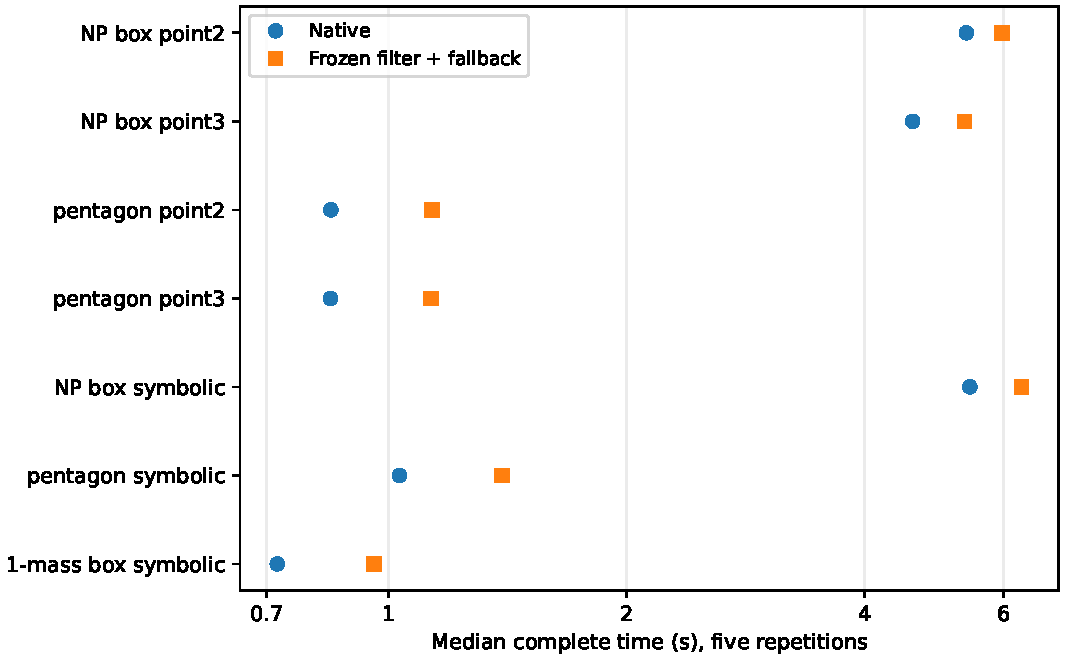
\includegraphics[width=\textwidth]{figures/generalization_times.pdf}
 \caption{Complete native and experimental learned-filter times on the
 new scattering batches. Each point is a median of five repetitions.
 The experimental time includes native fallback. Symbolic batches
 retain all invariants specified in the text.}
 \label{fig:generalization-times}
\end{figure}
The new application accepts symbolic family definitions and a supplied
master basis without reference target coefficients. It defaults to native
choices for these domains. The transfer measurements do not change the
earlier speedup estimates or activate a new learned route.
They provide explicit examples for later training on broader
scattering inputs~\cite{KiraGeneralizationData}.

\subsection{Physical IBP systems with a finite optimum}
A reverse construction supplies a valid path, while an optimality
claim also requires a defined cost and a complete comparison with
the allowed alternatives. We carry out that comparison on two
small systems with symbolic coefficients.
For the massless one-loop bubble, define
\begin{equation}
 B_{a,b}=\int\frac{d^d\ell}{\mathrm{i}\pi^{d/2}}\,
 \frac{1}{(\ell^2+\mathrm{i}0)^a
 [(\ell-p)^2+\mathrm{i}0]^b},\qquad p^2=s.
\end{equation}
Differentiation with the vectors $\ell$ and $\ell-p$ gives
\begin{align}
 0&=(d-2a-b)B_{a,b}-bB_{a-1,b+1}+bsB_{a,b+1},\\
 0&=(d-a-2b)B_{a,b}-aB_{a+1,b-1}+asB_{a+1,b}.
 \label{eq:general-bubble-ibp}
\end{align}
The massless one-denominator integrals vanish in dimensional
regularization. Selecting both operators at seed $(1,1)$, the first
at $(2,1)$ and the second at $(1,2)$ gives the closed system
\begin{equation}
 \begin{pmatrix}
 0&s&0&d-3\\
 s&0&0&d-3\\
 d-5&-1&s&0\\
 -1&d-5&s&0
 \end{pmatrix}
 \begin{pmatrix}B_{2,1}\\B_{1,2}\\B_{2,2}\\B_{1,1}\end{pmatrix}=0.
 \label{eq:general-bubble-matrix}
\end{equation}
We protect $B_{1,1}$ as the master and reduce the other three integrals
over $\mathbb Q(d,s)$. Their exact coefficients are
\begin{equation}
 B_{2,1}=B_{1,2}=\frac{3-d}{s}B_{1,1},\qquad
 B_{2,2}=\frac{(d-6)(d-3)}{s^2}B_{1,1}.
\end{equation}
An independent check obtains the same ratios from the
gamma-function expression for the bubble.

For a one-loop massive tadpole, define
\[
 T_a=\int\frac{d^d\ell}{\mathrm{i}\pi^{d/2}}\,
       (\ell^2-m^2+\mathrm{i}0)^{-a}.
\]
The IBP identity with vector $\ell$ is
\begin{equation}
 (d-2a)T_a-2am^2T_{a+1}=0.
 \label{eq:general-tadpole-ibp}
\end{equation}
Seeds $a=1,2,3$ give three equations for $T_2,T_3,T_4$ with master
$T_1$ over $\mathbb Q(d,m^2)$.
Native Kira reductions generated from the physical denominators
provide an additional check of both systems.

At a matrix state $S$, an allowed action chooses any nonzero entry
in an unprocessed row and an unprocessed nonmaster column.
It moves that row to the next pivot position, normalizes it and
eliminates the chosen column from every other row.
The master column remains protected, and each action removes one
nonmaster column from future pivot choices.
There are three pivot stages in each system.

We count one division for each nonzero nonpivot source entry when
the pivot differs from one. Each update of a nonpivot source entry
counts one multiplication and one subtraction.
Assignments, comparisons, structural cancellation of the pivot,
and polynomial operations inside a rational-function operation
are outside this cost. Thus the objective measures specified
coefficient operations, with no claim that each operation takes
the same time.

For this action set, define the remaining minimum cost by
\begin{equation}
 V(S)=\min_{a\in\mathcal A(S)}
       \bigl[c(S,a)+V(S_a)\bigr],\qquad V(S_{\rm done})=0.
 \label{eq:general-bellman}
\end{equation}
Here $\mathcal A(S)$ is the complete set of allowed pivots,
$c(S,a)$ is the counted cost, and $S_a$ is the exact next matrix.
We evaluate every alternative and retain the state graph,
using the finite recurrence of dynamic programming~\cite{Bellman1952}.
An independent checker reconstructs every row operation, checks
all outgoing actions, verifies the cost recurrence, and checks
the final master coefficients.
Since each action reduces the number of remaining columns,
induction from the terminal states proves the minimum for
the full stated path space.

To include initial equation selection, we also examine every subset
$\mathcal E$ of the saved source pool whose nonmaster matrix has rank
three. Each subset starts its own complete pivot search, giving
\begin{equation}
 C_{\rm pool}^{*}=
 \min_{\substack{\mathcal E\subseteq\mathcal E_{\rm full}\\
                 \operatorname{rank}A_{\mathcal E}=3}}
 V(S_{\mathcal E}).
 \label{eq:general-pool-optimum}
\end{equation}
Here $A_{\mathcal E}$ contains the nonmaster coefficients, and
$S_{\mathcal E}$ is the starting matrix for that subset.
Initial row selection carries no coefficient-operation cost in
this objective. The certificate records every sufficient subset
and every subsequent pivot choice.

The massless bubble certificate contains 113 distinct states and checks 234 transitions. It covers 152 complete paths across 5 sufficient source subsets. The minimum is 7 coefficient operations when initial equation selection is allowed, and 13 when the full source pool is retained.

The massive tadpole certificate contains 24 distinct states and checks 32 transitions. It covers 15 complete paths across one sufficient source subset. The minimum is 7 coefficient operations when initial equation selection is allowed, and 7 when the full source pool is retained.

The fixed control chooses the first available nonmaster column and then
the first available source row. It attains the full-pool minima
of thirteen and seven operations. A control that minimizes only the
immediate step cost uses thirteen operations for the bubble and nine
for the tadpole. Thus immediate cost can give a larger complete
cost even in a three-column physical system.
The minimum sufficient equation count is three for each pool,
with two distinct bubble seeds and three tadpole seeds.
All exact state transitions and terminal coefficients pass
independent checks, and six native Kira master coefficients agree
with the two symbolic systems.

The subset checks also certify the smallest sufficient equation count
and the smallest number of distinct source-seed labels within each saved
pool. These records give exact cost labels for later model tests.
The certificates apply to the displayed systems, protected masters,
allowed operations and cost definition. They do not establish an
optimum over additional IBP identities, changes of master basis,
other algebraic algorithms or unrestricted scattering reductions.
General high-loop scattering and wall-time optimality therefore
remain separate questions.
\FloatBarrier


\clearpage
% BEGIN CURRENT WORKFLOW UPDATE
\providecommand{\StudySection}{\section}
\providecommand{\StudySubsection}{\subsection}

\StudySection{Learning from complete reduction time}
\label{sec:workflow}
The scattering test shows why a useful equation label is an incomplete training objective for acceleration. A filter can retain sufficient equations and still add more overhead than it saves. We therefore train a model to predict complete reduction time and let it choose the initial seed region, an optional seed or equation filter, and an integral ordering. The model makes one choice for the whole target batch before Kira begins its exact calculation.

To evaluate that choice fairly, we also need a baseline with the same surrounding implementation. We combine the earlier equation filter with an existing improvement in temporary data handling, which reduces execution cost without changing the equations or arithmetic. The \emph{integrated native control} uses this implementation with Kira's own decisions. Comparing the learned strategy with that control measures the benefit of the prediction beyond the shared implementation changes.

For a target batch, let $B=(r_{\max},s_{\max},q_{\max})$ contain the largest positive index sum, numerator rank, and dot count. A dot is one denominator power above one. Table~\ref{tab:workflow-actions} lists the strategies considered, and Appendix~\ref{app:workflow} defines the quantities and derives the cost models. The seed limits and ordering options are provided by Kira~\cite{Kira12}; ordering five changes the priority of sectors while retaining the within-sector preference of ordering one. All strategies must return the same prescribed master basis.

\begin{table}[!htbp]
\centering\small
\caption{Strategies available to the complete-time model. Negative seed
bounds are replaced by zero. Native row choices remain active.}
\label{tab:workflow-actions}
\begin{tabular}{@{}ll@{}}\toprule
Strategy & Initial seed region and selection\\\midrule
Integrated native & Bounds $B$; native choices\\
Smaller region & Bounds $B-(1,1,1)$; native choices\\
Fewer dots & Bounds $B-(1,0,1)$; native choices\\
Equation filter & Bounds $B$; saved equation tree\\
Seed filter & Bounds $B$; saved seed tree where available\\
Different ordering & Bounds $B$; Kira ordering five\\
Larger region & Bounds $B+(1,1,1)$; native choices\\\bottomrule
\end{tabular}
\end{table}

A smaller region can avoid unnecessary equation generation, while a larger region can avoid a failed first attempt when the target's own index limits are insufficient. If the initial strategy fails the basis check, the calculation tries native choices at $B$ and then at $B+(1,1,1)$ when needed. The native control also enlarges an insufficient region, and every failed attempt contributes to the training and test time. For the four earlier multiloop graphs, the seed-filter option uses native choices because this implementation has no separate seed tree for them. Its equation-filter option uses the earlier trees for those graphs and the newly trained trees for the three additional scattering structures.

The model receives eighteen features describing the graph, symbolic variables, number of targets, index powers, and sectors. For each strategy, its training label is the logarithm of the complete-time ratio to integrated native choices. We compare a constant predictor, six regression trees, three ridge-regression models, and two nearest-neighbour models. Regression trees follow the squared-error construction of Ref.~\cite{CART1984}; Appendix~\ref{app:workflow} specifies all candidates. Validation selects ridge regression with penalty $\lambda=10$ and decision margin $\gamma=0$, giving validation ratio $0.993$.

The best fixed strategy selected from training is integrated native reduction. Consequently, the integrated-native and best-fixed controls use the same settings in independent trials, and differences between their times indicate execution variation. The seed and equation trees retain their earlier weights throughout this study, and learned row selection remains disabled.

The data contain 31 training batches, 17 validation batches, and 31 test batches from the sunrise, planar box, three-loop vacuum, three-loop ladder, nonplanar box, pentagon, and box with external virtuality. Rational batches use different masses or invariants across the splits, while additional symbolic batches use different target lists. These are new inputs within seven known graph structures at one through three loops. The recurrence study through twelve loops remains a separate result for its restricted vacuum family.

Each training and validation cost uses three repetitions. Testing uses five repetitions to compare the preceding native implementation, integrated native choices, the best fixed strategy, and the learned strategy. The controller and models are loaded before timing, but every attempt starts a fresh Kira process. Timers include input preparation, prediction, native IBP generation, algebra, exact checks, cleanup, and retries. They exclude training, enlarged reference reductions, and later recording of results. Additional application checks measure cold startup and compare returned coefficients after a reduction supplied only with its targets and basis. For an unknown graph or target complexity outside the training range, the learned application uses native choices; the same guard applies to combined requests.

\StudySubsection{Results for individual target batches}
All 620 timed calculations pass exact checks of 59,640 coefficient entries, and all 31 applications supplied without reference coefficients pass their subsequent comparisons. Each timed method makes fifteen fallback attempts. Thus this model changes some initial strategies but does not remove the remaining cases that need a second attempt.

Relative to the preceding native implementation, the learned strategy has time ratio $0.9903$, with descriptive interval $[0.9796,0.9996]$, or about 1.0\% less time. Its ratio to integrated native choices is $0.9965$ with interval $[0.9875,1.0070]$, and its ratio to the best-fixed control is $1.0026$ with interval $[0.9979,1.0081]$. Both comparisons with the matched integrated controls include equal time. They therefore provide no reliable additional saving from the learned choices. The two identically configured controls have ratios $0.9938$ and $0.9878$ to the preceding native implementation, illustrating the scale of execution variation.

Table~\ref{tab:workflow-times} reports the results by graph. The aggregate averages logarithmic ratios within each graph and then gives all seven graphs equal weight, as derived in Appendix~\ref{app:workflow}. The smallest learned-to-native ratio is $0.9654$ for the three-loop vacuum, while the ladder and nonplanar box take slightly more time. These results motivate testing more specific strategies for each graph rather than enabling the common model for all inputs.

\begin{table}[!htbp]
\centering\small
\caption{Complete-cost results. Native seconds are geometric means of
batch median times. The other entries are geometric mean time ratios;
a value below one means less time.}
\label{tab:workflow-times}
\begin{tabular}{@{}lrrrr@{}}\toprule
Graph & Native (s) & Integrated/native & Learned/native & Learned/integrated\\\midrule
Sunrise & 0.502 & 1.0123 & 0.9932 & 0.9811\\
Planar box & 1.621 & 0.9906 & 0.9771 & 0.9864\\
Three-loop vacuum & 0.726 & 0.9745 & 0.9654 & 0.9907\\
Three-loop ladder & 3.535 & 1.0146 & 1.0013 & 0.9869\\
Nonplanar box & 3.119 & 1.0075 & 1.0073 & 0.9998\\
Pentagon & 0.599 & 0.9758 & 0.9942 & 1.0189\\
Box with virtuality & 0.484 & 0.9824 & 0.9944 & 1.0122\\
\bottomrule
\end{tabular}
\end{table}

\begin{figure}[!htbp]
\centering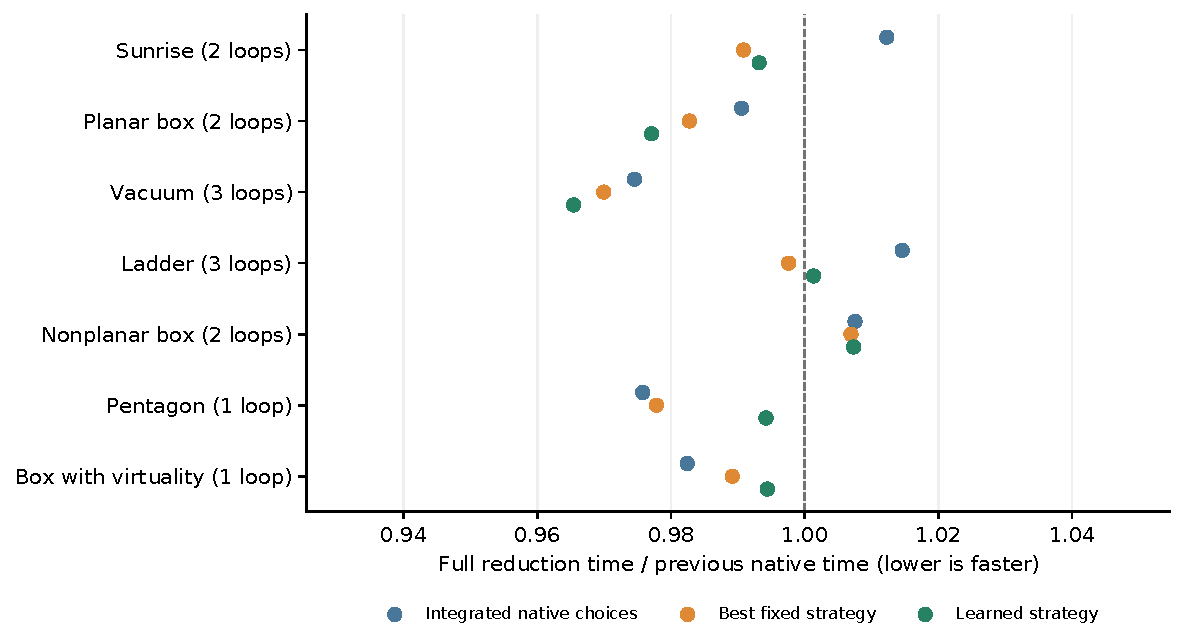
\includegraphics[width=\linewidth]{paper_figures/workflow_time.pdf}
\caption{Learned choices and the native controls have similar complete times.
The best-fixed and integrated controls use the same configuration in
separate trials. The plot shows variation across graph structures;
the text gives the aggregate uncertainty intervals. The axis focuses
on the measured range and retains the equal-time line.}
\label{fig:workflow}
\end{figure}

\FloatBarrier

\StudySubsection{Sharing a reduction between compatible requests}
Before changing the predictor, we test whether repeated work can be removed from the way Kira receives targets. When two available requests have the same family and kinematics, their target lists can be combined and reduced together. The resulting coefficient rows are then returned to the appropriate request. This shares family preparation and algebra between the lists. Appendix~\ref{app:workflow} defines the ten request groups and derives this separation from linearity; the model and its settings remain fixed.

Five repetitions of four methods give 200 complete calculations, all of which pass exact checks. Joint native reduction has ratio $0.5252$ to two separate native reductions. With the integrated implementation and native choices, the ratio is $0.5175$ with interval $[0.5073,0.5346]$, giving 48.3\% less time or speedup $1.93$ with interval $[1.87,1.97]$. Every tested graph group benefits from the shared reduction. Its integrated-native ratios range from $0.5040$ to $0.5679$, corresponding to savings of 43.2--49.6\%.

The joint learned strategy has ratio $0.5152$ to separate native requests, but its ratio to joint integrated native choices is $0.9955$ with interval $[0.9810,1.0058]$. As Table~\ref{tab:joint} and Figure~\ref{fig:joint} show, the main gain comes from sharing the calculation; the predictor adds no reliable improvement over the matched joint control. The standard application therefore uses the fixed strategy selected from training, which retains native choices. Ten checks of each joint application and ten checks of the single-batch application supply only a basis and verify the returned coefficients independently, in addition to the 31 application checks above.

\begin{table}[!htbp]
\centering\small
\caption{Joint-request time ratios and descriptive intervals over the
seven graph groups. Each group contains two compatible target requests.}
\label{tab:joint}
\begin{tabular}{@{}lrr@{}}\toprule
Comparison & Time ratio & 95\% interval\\\midrule
Joint native / separate native & 0.5252 & $[0.5130,0.5420]$\\
Joint integrated / separate native & 0.5175 & $[0.5073,0.5346]$\\
Joint learned / separate native & 0.5152 & $[0.5022,0.5322]$\\
Joint learned / joint native & 0.9810 & $[0.9657,0.9946]$\\
Joint learned / joint integrated & 0.9955 & $[0.9810,1.0058]$\\
\bottomrule
\end{tabular}
\end{table}

\begin{figure}[!htbp]
\centering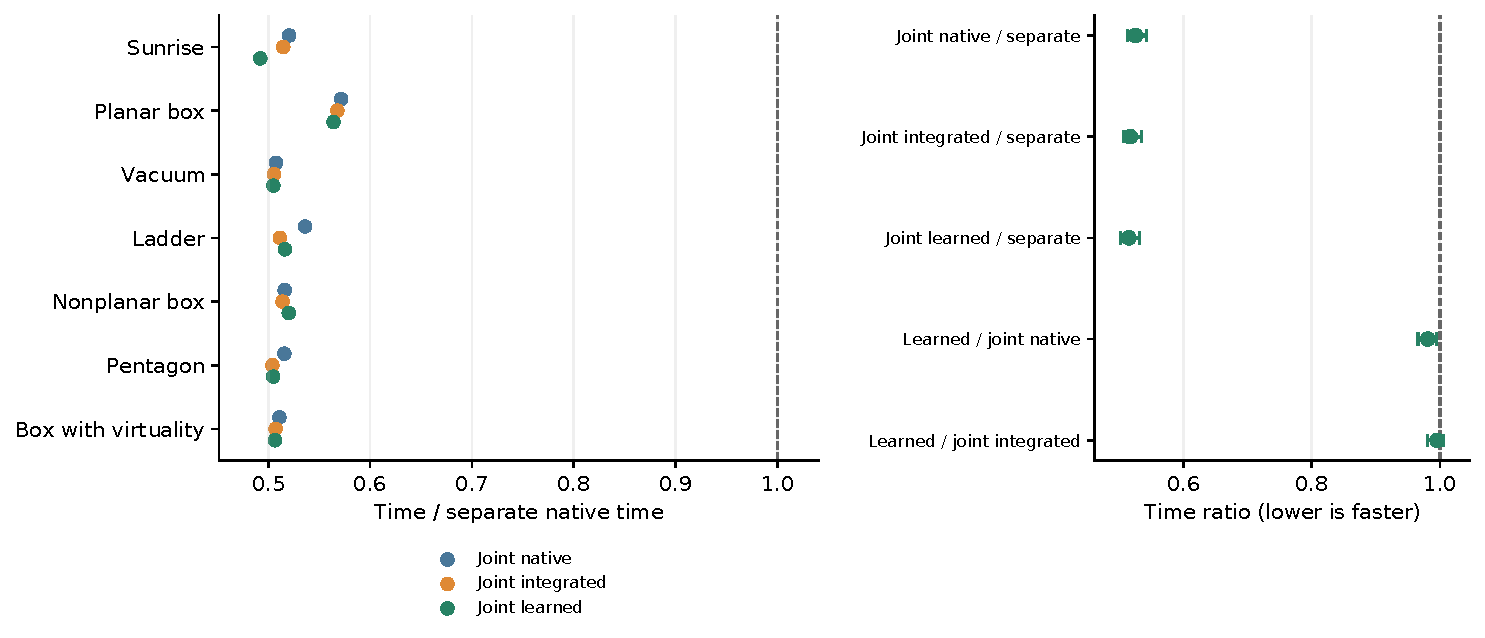
\includegraphics[width=\linewidth]{paper_figures/request_batching.pdf}
\caption{Combining compatible requests gives the main saving.
Left: ratios by graph relative to two separate native reductions.
Right: aggregate ratios and descriptive intervals. Comparing learned
choices with joint integrated native choices gives no reliable extra
saving. The panels retain the equal-time reference.}
\label{fig:joint}
\end{figure}

\FloatBarrier

The joint comparison reuses the main test's reserved parameter points, so it provides an additional comparison on that population. Its saving requires requests that can share one calculation. Transfer to new graph structures, isolated arbitrary integrals, and general scattering beyond three loops remains outside this result. The next study returns to individual batches and tests whether separate models and a wider set of seed strategies give a measurable gain.

\providecommand{\StudySection}{\section}
\providecommand{\StudySubsection}{\subsection}

\StudySection{Choosing a strategy separately for each graph}
\label{sec:type-specialists}
A common predictor may miss differences in the work required by different graph structures. We therefore fit separate predictors for the seven graphs and enlarge the available seed strategies. The added choices can restrict seeding to maximal target sectors or reduce numerator seeding in lower sectors through Kira's truncation option~\cite{Kira3}. Each method first enforces a valid positive-index bound for its declared sectors, and the final basis check and fallback remain in place.

For each graph, ten candidate models predict the complete-time ratios of nine strategies from nine target and family features. The candidates include regression trees, a bagged ensemble of trees, regularized linear models, and nearest-neighbour models. Their cost labels include unsuccessful attempts and retries. The data contain 36 training batches, 18 validation batches, and 36 reserved test batches at new rational parameter values, with $d$ symbolic throughout. Targets include propagator powers up to three, lower sectors, and auxiliary numerator indices $-2$. Appendix~\ref{app:type-specialists} gives the exact input definitions and selection procedure.

Training and validation contain 2,798.5 seconds of measured reductions, while fitting all seventy candidates takes 0.86 seconds. These offline costs exclude reference construction, development, and replaced measurements and are not included in application time. Validation enables a new predictor only if it saves at least five percent against the fastest available control. The controls are native choices, a deterministic sector-and-truncation rule, and a fixed strategy for each graph selected from training; the fixed strategy may itself use the older equation filter. This requirement activates predictors for three graphs and retains a control for the others. Unknown graphs and features outside the training range use native choices.

Five repetitions of four methods give 720 test calculations, all of which pass exact coefficient checks. With equal weight for each graph, the selected method has ratio $0.9368$ to native choices, with descriptive interval $[0.8867,0.9878]$, corresponding to 6.3\% less time. Its ratio to a fixed strategy for each graph is $0.9441$ with interval $[0.8992,0.9863]$. This second comparison isolates the benefit of selecting a strategy from the targets beyond choosing one setting for the whole graph.

Table~\ref{tab:type-specialists} shows lower time for five of the seven groups. The enabled trees save 14.2\% for the planar box, 12.4\% for the ladder, and 13.8\% for the nonplanar box. The vacuum and box with external virtuality take 3.7\% and 0.8\% more time, respectively, while retaining control strategies throughout. In particular, the vacuum uses native settings, so its difference includes the extra selection overhead and execution variation. Across 180 timed trials, the selected method needs no retries and native choices require 40; these costs are included in the ratios.

\begin{table}[!htbp]
\centering\small
\caption{Reduction time with a separate strategy for each graph. Times are geometric means of batch medians in seconds, and the ratio divides selected time by native time. The strategy column identifies the enabled model or retained control.}
\label{tab:type-specialists}
\begin{tabular}{@{}llrrr@{}}\toprule
Graph & Strategy & Native & Selected & Ratio\\\midrule
Sunrise & Stronger truncation & 0.825 & 0.811 & 0.983\\
Planar box & Depth-two tree & 3.410 & 2.925 & 0.858\\
Vacuum & Native & 1.033 & 1.072 & 1.037\\
Ladder & Depth-one tree & 5.144 & 4.506 & 0.876\\
Nonplanar box & Depth-two tree & 6.234 & 5.376 & 0.862\\
Pentagon & Target sectors & 1.040 & 0.989 & 0.951\\
Virtuality box & Sectors and truncation & 0.808 & 0.815 & 1.008\\
\bottomrule\end{tabular}
\end{table}

\begin{figure}[!htbp]
\centering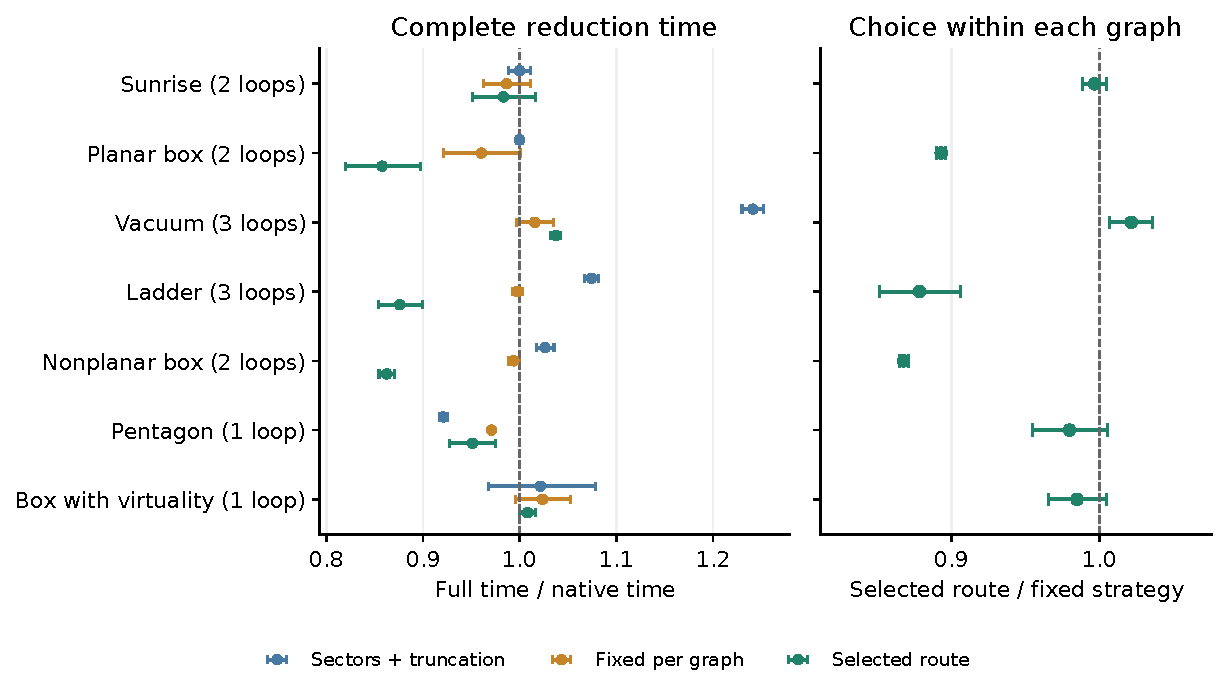
\includegraphics[width=\linewidth]{paper_figures/type_specialists.pdf}
\caption{The effect of choosing a separate policy for each graph.
Left: complete-time ratios to native choices. Right: the selected method
relative to one fixed strategy per graph. Bars show the range across two
reserved parameter profiles; they are not significance intervals.
Both panels retain the equal-time reference.}
\label{fig:type-specialists}
\end{figure}

\FloatBarrier

The timed trials check 14,040 coefficient entries. A further 36 applications supplied only with the master basis and seven additional application checks verify 945 coefficients independently. These checks establish correct completion for the measured inputs. The graph structures and target patterns are known during training, and each graph has only two training parameter profiles. The reserved profiles therefore test new kinematic values within these inputs, leaving new target structures and general scattering beyond three loops for further study.

\providecommand{\StudySection}{\section}
\providecommand{\StudySubsection}{\subsection}

\StudySection{Expanding seeds selectively and using an intermediate basis}
\label{sec:basis-completion}
The graph-specific study identifies symbolic equation regeneration as the largest measured solver stage. Some target batches need seed limits beyond those of the targets themselves, and a general enlargement can generate many unnecessary equations. We therefore test whether selective increases in the limits, or a reduction through an intermediate master basis, can lower this remaining cost.

The candidate set contains six ways to increase selected seed limits and two ways to reduce first to a temporary basis. In the latter case, Kira reduces the remaining temporary masters to the prescribed basis, and exact multiplication combines the two coefficient matrices. The final basis requirement is the same for every method. Appendix~\ref{app:basis-completion} defines the candidates and derives this conversion, which allows the first target reduction to use a smaller system when the remaining basis conversion is inexpensive.

For development batch $c$, let $B_c=(r_c,s_c,q_c)$ denote valid initial limits on the positive index sum, numerator rank, and number of extra denominator powers. We retain the fastest new candidate for a development batch only if it saves at least ten percent against the graph-specific method in Section~\ref{sec:type-specialists}. The resulting candidate set contains that preceding method, full-sector basis completion, and the selective increments $B_c+(1,0,0)$, $B_c+(0,1,0)$, and $B_c+(1,1,0)$. Development results select the options but do not enter the reserved comparison.

The new data contain 36 training batches, 18 validation batches, and 36 test batches from the same seven graphs and target patterns, with new rational kinematics and symbolic $d$. Ten predictors per graph use the same nine features to predict time relative to the preceding method. Validation compares each predictor with that method and with a fixed new strategy selected from training for each graph. A predictor is enabled only if it saves at least five percent against the faster control; otherwise that control is used. A fixed candidate may itself call the preceding learned method, so this comparison tests the additional choice among the new options.

Validation enables new predictors for three graphs. The retained training and validation records contain 1,731.7 seconds of measured reductions, and fitting the seventy candidates takes 0.88 seconds. These costs exclude reference construction and development and remain outside the reserved reduction timer.

The test compares native choices, the preceding graph-specific method, the new fixed strategy, and the selected strategy. Five repetitions give 720 calculations, all of which pass exact checks. A further 43 applications also pass when the reduction receives no target reference coefficients. With equal weight for each graph, the selected method has ratio $0.9115$ to the preceding method, with descriptive interval $[0.8105,0.9980]$, giving 8.8\% less time. Its ratio to native choices in the same experiment is $0.8516$ with interval $[0.7282,0.9647]$, giving 14.8\% less time. Relative to the new fixed strategy, the ratio is $0.9264$ with interval $[0.8760,0.9747]$.

The sum of batch medians answers a different question: how long would this set of requests take when each is counted once? For the 36 reserved batches, this sum is 106.24 seconds for native choices, 96.32 seconds for the preceding method, and 77.03 seconds for the selected method. The geometric ratios above instead give every graph equal weight. Both measures show a saving, although their magnitudes differ because the longer calculations contribute more to the workload total.

The stage measurements explain where part of the saving occurs. Across 180 runs per method, symbolic equation regeneration falls from 138.02 to 80.58 seconds. Neither the preceding nor the selected method makes a fallback attempt, compared with 40 for native choices. Planned second-stage reductions of temporary masters are included in complete time and are counted separately from fallback. The comparison with the fixed strategy supports an additional benefit from the selection procedure, which combines validation-based control choices with predictions for individual target batches.

\begin{table}[!htbp]
\centering\small
\caption{Selective seed expansion compared with the graph-specific method in Section~\ref{sec:type-specialists}. Times are geometric means of batch medians in seconds. ``Previous'' denotes that graph-specific method and ``New'' denotes the seed-expansion method. Each graph has two reserved parameter profiles.}
\label{tab:basis-completion}
\begin{tabular}{@{}llrrrr@{}}\toprule
Graph & Policy & Previous (s) & New (s) & New/previous & New/native\\\midrule
Sunrise & Add $s$ & 0.596 & 0.593 & 0.995 & 0.979\\
Planar box & Tree depth 1 & 2.422 & 2.062 & 0.851 & 0.735\\
Vacuum & Complete basis & 0.928 & 0.941 & 1.013 & 1.016\\
Ladder & Tree depth 1 & 4.477 & 3.007 & 0.672 & 0.584\\
Nonplanar box & Tree depth 1 & 4.091 & 3.550 & 0.868 & 0.759\\
Pentagon & Previous & 0.723 & 0.754 & 1.043 & 0.998\\
Virtuality box & Previous & 0.580 & 0.582 & 1.003 & 1.004\\
\bottomrule\end{tabular}
\end{table}

\begin{figure}[!htbp]
\centering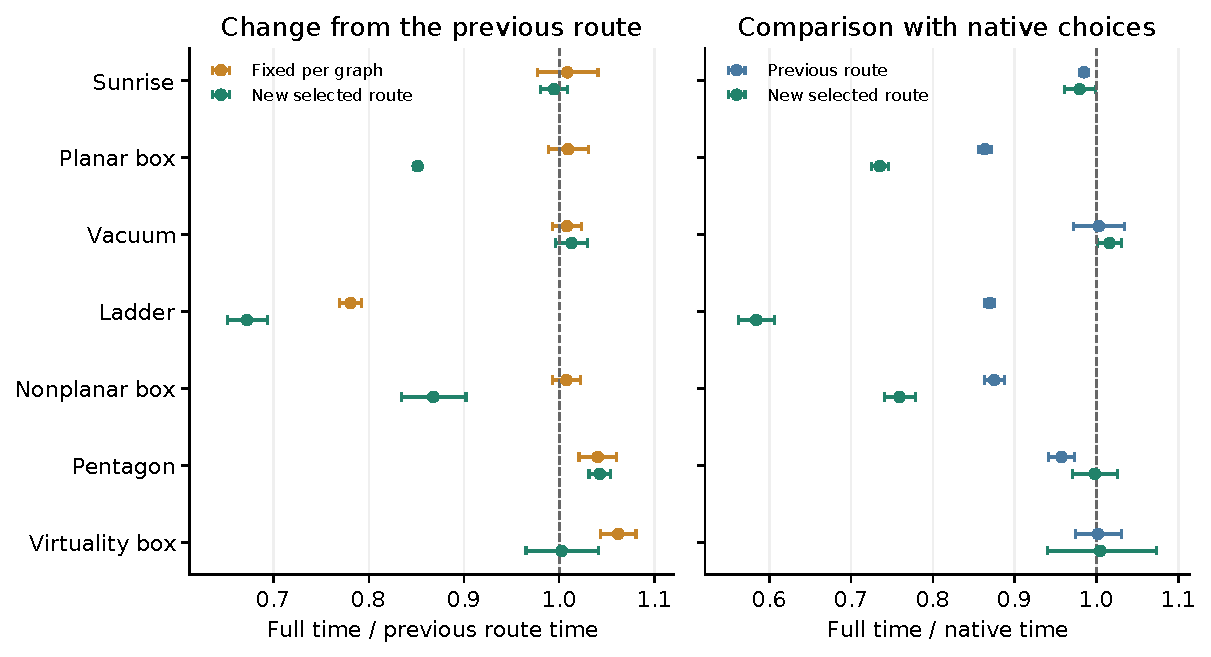
\includegraphics[width=\linewidth]{paper_figures/basis_completion.pdf}
\caption{Selective choices change complete reduction time. Left: the new
fixed strategy and selected method relative to the preceding method.
Right: the preceding and new methods relative to native choices in the
same test. Values below one are faster. Bars show the range over the two
reserved profiles; they are not significance intervals.}
\label{fig:basis-completion}
\end{figure}

\FloatBarrier

The gain is not uniform across the graphs. Relative to the preceding method, the vacuum takes 1.3\% more time, the pentagon 4.3\% more, and the box with external virtuality 0.3\% more. All reported times include prediction, native IBP generation, basis conversion, exact algebra, checks, cleanup, and fallback. These results measure the additional method directly on new parameter profiles; they do not multiply gains from earlier experiments. Their scope remains known graphs and target patterns with rational kinematics, rather than unrestricted symbolic kinematics or arbitrary high-loop scattering.

\providecommand{\StudySection}{\section}
\providecommand{\StudySubsection}{\subsection}

\StudySection{Testing integral and propagator orderings}
\label{sec:ordering-policy}
Selective seed expansion reduces equation-generation work, but the ordering of the resulting integrals can still affect elimination. Kira provides eight integral priority rules and four automatic propagator-ordering schemes~\cite{Kira12,Kira3}. We test whether a model can choose among these settings from the target indices before equation generation, while retaining the seed strategy from Section~\ref{sec:basis-completion}. The model makes one decision for each batch, and a failed basis check triggers a repeat with the preceding settings. Appendix~\ref{app:ordering-policy} defines the candidates and shows why consistent relabelling preserves the integrals.

Development first compares eleven candidates and then tests the pair of best nondefault orderings for each batch. We keep the preceding settings and any batch winner that saves at least ten percent of complete time. If $\omega$ is the integral-order number and $\chi$ the propagator-scheme number, the retained new settings are $(\omega,\chi)=(2,1)$, $(7,1)$, $(5,4)$, and $(8,3)$. The preceding method also remains available without a change in its settings.

We fit ten predictors per graph on 36 training batches, select their use on 18 validation batches, and test on 36 reserved batches. The features, complete-time labels, candidate model types, and five-percent validation requirement are the same as in the seed-expansion study. A fixed ordering still uses the preceding learned seed strategy, so the fixed-setting comparison measures the additional ordering decision. Training and validation contain 1,432.8 seconds of reductions, and fitting the seventy predictors takes 0.93 seconds. These offline costs exclude development and reference construction.

None of the predictors passes the validation requirement. The tested selected method therefore uses fixed ordering settings chosen by validation, with no newly enabled ordering predictor. Any difference in its time reflects those settings, their interaction with the retained seed strategy, and execution variation. This distinction is necessary when interpreting the results as evidence about machine learning.

All 720 timed reductions and 43 additional applications pass exact checks; the additional applications receive no target reference coefficients during reduction. With equal weight for each graph, the selected-to-preceding ratio is $1.0141$ with descriptive interval $[0.9986,1.0303]$, giving 1.4\% more time. The selected-to-native ratio is $0.8499$ with interval $[0.7306,0.9642]$, giving 15.0\% less time, while the ratio to the new fixed strategy is $1.0070$ with interval $[0.9811,1.0327]$. The saving against native choices therefore does not show an improvement over the already learned seed-expansion method.

The sum of median times over the 36 test batches is 110.09 seconds for native choices, 79.61 seconds for the preceding method, 79.53 seconds for the new fixed settings, and 79.68 seconds for the selected settings. On this workload, the selected method takes 0.1\% more time than its predecessor. Its additional ordering decision takes a median of 271.1 microseconds per application, and both this cost and the retained seed-policy cost are included in complete time.

\begin{table}[!htbp]
\centering\small
\caption{Ordering settings compared with the seed-expansion method in Section~\ref{sec:basis-completion}. Times are geometric means of batch medians in seconds. ``Previous'' retains the earlier ordering, and ``New'' uses the selected setting. The pair $(\omega,\chi)$ specifies the integral order and propagator scheme.}
\label{tab:ordering-policy}
\begin{tabular}{@{}llrrrr@{}}\toprule
Graph & Choice & Previous (s) & New (s) & New/previous & New/native\\\midrule
Sunrise & $(7,1)$ & 0.610 & 0.633 & 1.037 & 1.034\\
Planar box & $(2,1)$ & 2.407 & 2.390 & 0.993 & 0.759\\
Vacuum & Previous & 0.975 & 0.982 & 1.007 & 0.983\\
Ladder & Previous & 3.122 & 3.088 & 0.989 & 0.591\\
Nonplanar box & $(2,1)$ & 3.698 & 3.681 & 0.995 & 0.745\\
Pentagon & $(2,1)$ & 0.788 & 0.820 & 1.041 & 0.987\\
Virtuality box & $(5,4)$ & 0.601 & 0.624 & 1.039 & 0.955\\
\bottomrule\end{tabular}
\end{table}

\begin{figure}[!htbp]
\centering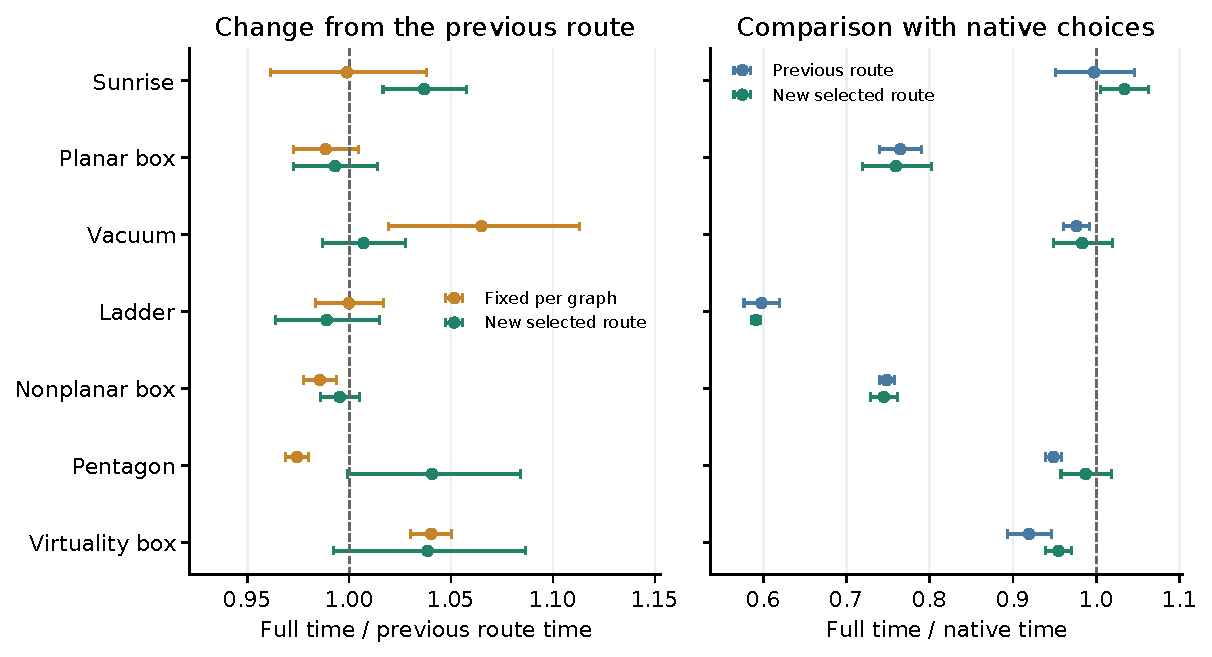
\includegraphics[width=\linewidth]{paper_figures/ordering_policy.pdf}
\caption{The effect of choosing Kira settings before reduction. Left:
new fixed settings and selected settings relative to the preceding method.
Right: preceding and selected methods relative to native choices.
Values below one indicate less complete time. Bars give the range across
two parameter profiles; they are not significance intervals.}
\label{fig:ordering-policy}
\end{figure}

\FloatBarrier

The sunrise, vacuum, pentagon, and box with external virtuality take 3.7\%, 0.7\%, 4.1\%, and 3.9\% more time, respectively. No selected calculation requires fallback. Across 180 runs per method, symbolic equation regeneration changes from 79.88 to 80.58 seconds, while back-substitution changes from 37.99 to 37.35 seconds. These stage measurements show small changes in opposite directions rather than a consistent overall improvement.

The timers include prediction, preparation, native generation, exact checks, basis conversion, retries, and cleanup. As in the preceding comparisons, the caller and models are already loaded, and each attempt starts a fresh Kira process. The evidence therefore supports retaining the earlier ordering for this measured workload of known one- through three-loop graphs at new rational parameter values. The next comparison keeps that choice and changes the amount of parallel work instead.

\providecommand{\StudySection}{\section}
\providecommand{\StudySubsection}{\subsection}

\StudySection{Choosing how many Kira workers to use}
\label{sec:thread-policy}
The ordering study gives no further saving, so we retain the seed-expansion method and its earlier ordering. We next test the number of Kira workers, which determines how much of the symbolic calculation can run in parallel~\cite{KiraOriginal}. Development measurements show that extra workers add overhead on small batches, while some larger box batches finish sooner. This suggests choosing the worker count from the requested targets before equation generation.

The candidate counts are one, two, and four workers in the same integrated executable. The native control uses Kira's own seed and reduction decisions together with the common earlier implementation changes. For the learned comparison, the nine target features used above predict each worker count's complete time relative to one worker. We fit ten predictor types per graph on 36 training batches, select settings on 18 validation batches, and reserve 36 more batches for testing. Validation minimizes the sum of batch median times. A predictor must save at least two percent against the faster control and give lower summed time in at least two of three validation repetitions; otherwise the control remains active. Appendix~\ref{app:thread-policy} gives the labels, checks, and comparison rules.

Validation enables a depth-two tree for the planar box and a depth-one tree for the nonplanar box. The other five graph types retain the preceding one-worker strategy. Both trees split only on the number of targets in the batch and choose at most two workers. Since the tested target patterns repeat across the parameter splits, these results establish a useful decision within those patterns; they do not establish target count as a sufficient description of arbitrary integral structures. Training and validation contain 1,098.1 seconds of reductions, and fitting all seventy candidates takes 0.82 seconds. These offline costs exclude reference construction and development.

All 900 timed reductions and 50 additional applications pass exact checks. The additional applications receive targets and a prescribed basis without reference coefficients. Seven run consecutively through a caller that keeps the models loaded, in a separate two-core allocation; each native attempt still starts a fresh Kira process. The timing experiment reserves four cores for every method so that the always-four-worker control can use its full setting. Thus every timed method has the same available resources, even when it uses fewer workers.

For the 36 reserved batches, the sum of median complete times falls from 82.21 seconds with the preceding one-worker method to 78.73 seconds with worker selection, a reduction of 4.2\%. In the same experiment, native one-worker choices take 110.67 seconds, always using four workers takes 156.95 seconds, and a fixed count for each graph takes 82.45 seconds. Selection therefore gives 4.5\% less time than the fixed-per-graph control. Table~\ref{tab:thread-policy} shows where these differences arise; changes for the five graphs that retain one worker include execution variation and the additional decision cost.

\begin{table}[!htbp]
\centering\small
\caption{Time with and without worker selection. Entries sum the batch median times within each graph, in seconds. ``Previous'' uses the seed-expansion method with one worker; ``Selected'' uses the validation-selected count. The final column divides selected time by previous time.}
\label{tab:thread-policy}
\begin{tabular}{@{}llrrr@{}}\toprule
Graph & Choice & Previous (s) & Selected (s) & Selected/previous\\\midrule
Sunrise & 1 worker & 5.271 & 5.215 & 0.989\\
Planar box & Tree depth 2 & 15.643 & 14.997 & 0.959\\
Vacuum & 1 worker & 4.813 & 4.620 & 0.960\\
Ladder & 1 worker & 23.197 & 23.602 & 1.017\\
Nonplanar box & Tree depth 1 & 26.768 & 23.819 & 0.890\\
Pentagon & 1 worker & 3.558 & 3.523 & 0.990\\
Virtuality box & 1 worker & 2.963 & 2.955 & 0.997\\
\bottomrule\end{tabular}
\end{table}

Giving each graph equal weight yields a smaller selected-to-preceding ratio of $0.9817$, with descriptive interval $[0.9682,0.9946]$, or 1.8\% less time. The selected-to-native ratio is $0.8456$ with interval $[0.7346,0.9502]$, or 15.4\% less time. These averages give equal importance to each graph, whereas the sum of medians measures the time for this particular collection of requests. Figure~\ref{fig:thread-policy} also shows why simply increasing every calculation to four workers is ineffective on these small cases.

\begin{figure}[!htbp]
\centering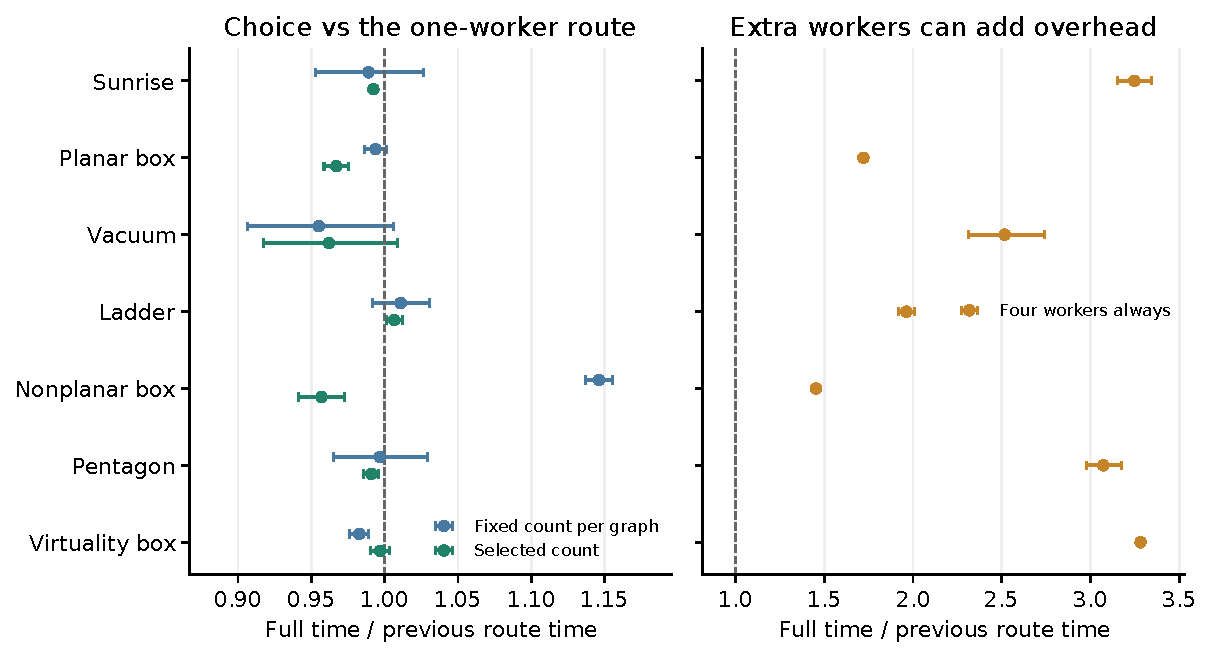
\includegraphics[width=\linewidth]{paper_figures/thread_policy.pdf}
\caption{The effect of selecting the worker count. Left: selected and fixed worker counts compared with the preceding
one-worker method. Right: always using four workers adds overhead on
many small cases. Each panel has its own horizontal scale.
Each point is the geometric mean of batch time ratios for one graph. Bars show the
range across two parameter profiles and are not significance intervals.}
\label{fig:thread-policy}
\end{figure}

\FloatBarrier

Variation between repetitions matters for the size of the gain. Across all five repetitions, the selected method takes 404.84 seconds and the preceding method 414.08 seconds, giving 2.2\% less elapsed time. Selection has lower summed time in four of the five repetitions, with selected-to-preceding ratios ranging from $0.9346$ to $1.0555$. This range describes the observed repetitions and is not a confidence interval. The ladder's sum of median times increases by 1.7\%.

The saving in elapsed time also uses more CPU time. The extra prediction takes a median of 276.6 microseconds and is included in the complete-time measurements. Across 180 reductions per method, the preceding strategy uses 385.9 CPU-seconds, the always-four-worker strategy 1024.1, and the selected strategy 458.9. Selection therefore increases CPU use by 18.9\%. These values measure CPU time consumed by the calculation, rather than the number of cores allocated to it.

The selected method has no failed attempts and requires no fallback. The always-four-worker method has ten unsuccessful native attempts, whose subsequent retries succeed; their costs remain in the reported time. Some native attempts report allocation failures under the imposed process limits. All comparisons include prediction, preparation, exact algebra, basis conversion, checks, retries, and cleanup, with the caller and models loaded before timing and a fresh Kira process for each attempt.

Worker selection is retained for this measured workload because it lowers elapsed time while preserving the exact results. Its demonstrated scope is seven known graph structures at one through three loops, known target patterns, and new rational kinematics with symbolic dimension. The preceding one-worker method remains available when the resource conditions or inputs differ. The result identifies a measured improvement among the tested choices, with the CPU cost stated alongside it.

\section{Checking the contribution of each component}
\label{sec:components}
The previous models form a sequence of choices, so a faster final calculation does not identify which choice supplies the saving. We compare ten methods on fourteen fresh batches from seven known graph structures and then disable individual learned decisions while keeping the other stages unchanged. Every method uses the same targets and prescribed basis. All 420 reductions in the first comparison and all 96 additional decision controls pass exact coefficient checks.

The native-choice total is 66.035 seconds, using sums of three-run batch medians. Table~\ref{tab:component-common} shows the complete strategies relative to that control. The result through worker selection takes 46.777 seconds, but this saving includes fixed seed settings as well as learned decisions. The equation, seed, and row filters increase time on this particular target pattern. Earlier savings on other targets remain separate results.

\begin{table}[!htbp]\centering\small
\caption{Component comparison on the same fourteen batches. Complete times include decisions, exact checks, and recovery. The first three rows retain preceding stages.}
\label{tab:component-common}
\begin{tabular}{@{}lrl@{}}\toprule
Method & Complete time (s) & Change from native\\\midrule
Graph-strategy model & 61.779 & 6.4\% less time\\
Through seed expansion & 49.309 & 25.3\% less time\\
Through worker selection & 46.777 & 29.2\% less time\\
Equation filter & 72.446 & 9.7\% more time\\
Seed filter & 70.241 & 6.4\% more time\\
Row model & 105.500 & 59.8\% more time\\
\bottomrule\end{tabular}\end{table}

\begin{table}[!htbp]\centering\small
\caption{The added learned decision, with other stages held fixed. Each row uses the subset on which that decision is enabled. Fixed settings were selected before this test.}
\label{tab:isolated-choices}
\begin{tabular}{@{}lrrrl@{}}\toprule
Decision & Batches & Fixed (s) & Learned (s) & Change\\\midrule
Graph choice & 6 & 51.448 & 50.188 & 2.4\% less time\\
Seed expansion & 6 & 41.030 & 41.093 & 0.2\% more time\\
Worker count & 4 & 24.232 & 25.555 & 5.5\% more time\\
\bottomrule\end{tabular}\end{table}

The isolated controls in Table~\ref{tab:isolated-choices} show why complete-time gains need a fixed comparison. On these batches, graph choice saves a small amount, while the added seed and worker choices increase time. Figure~\ref{fig:component-controls} presents both comparisons. These results motivate replacing the sequence of selectors with the single cost policy in the next section.

\begin{figure}[tbp]\centering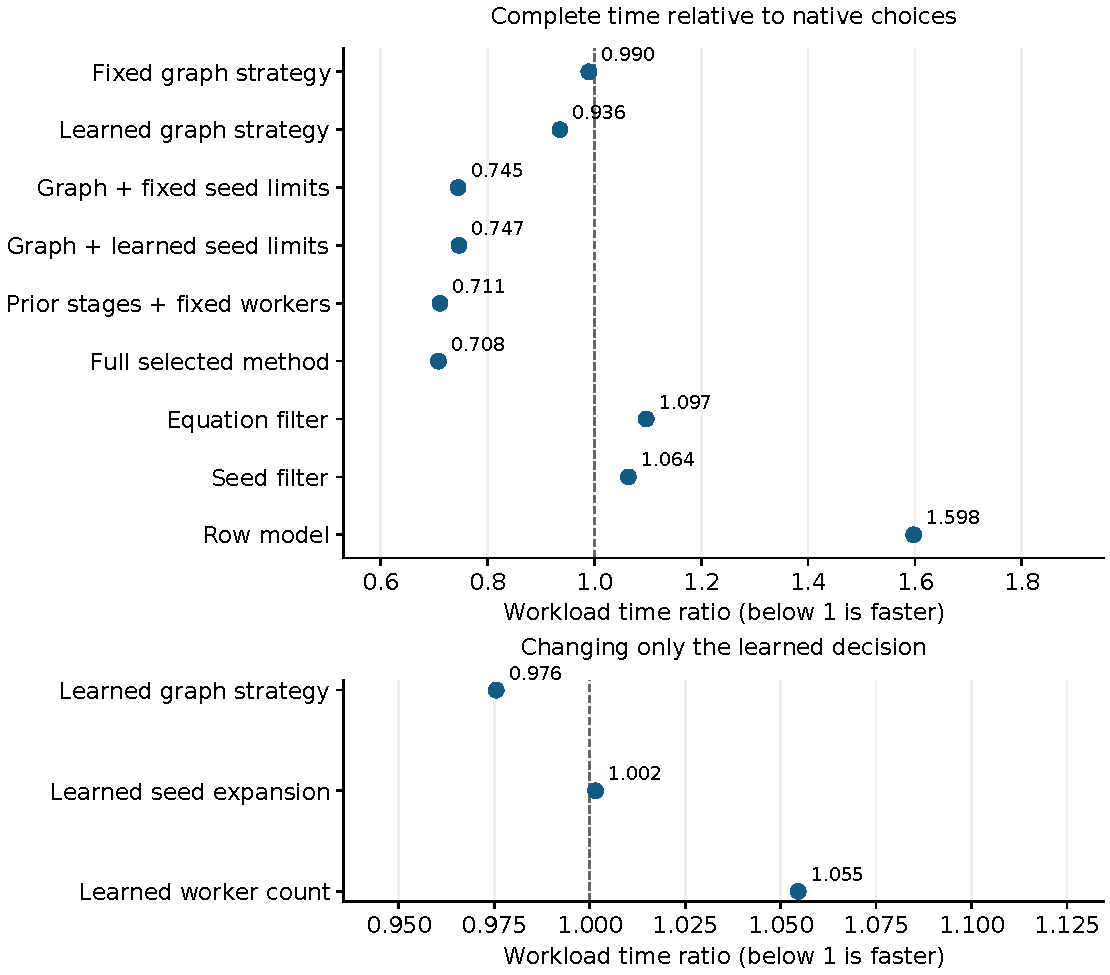
\includegraphics[width=\linewidth]{paper_figures/component_ablation.pdf}
\caption{Complete strategies and their added learned decisions. The upper panel uses all fourteen batches. The lower panel changes one learned decision on its enabled subset. Both show ratios of summed batch medians and retain the equal-time reference.}
\label{fig:component-controls}\end{figure}

\subsection{Connected scattering and bounded higher-loop tests}
We also construct connected four-point ladders and boxes with bubble subgraphs, defined in Appendix~\ref{app:higher-scattering}. The two completed three-loop bubble-box profiles take 10.538 seconds with restricted initialization and native equation choices, compared with 7.468 seconds with the frozen equation filter. This is 29.1\% less time under the same initialization. The complete strategy selectors otherwise retain native choices on these previously unsupported graph structures.

The bounded four- through six-loop probes identify separate costs and limits. Four-loop initialization exceeds the initial short time allowance. Five-loop attempts exceed the memory allowance, and the six-loop four-point representation requires 39 inverse propagators, above the tested executable's 31-entry limit. Later runs produce a four-loop bubble-box reference and reproduce its coefficients with enlarged seeds. Three native repetitions have median time 465.329 seconds. Two completed filtered repetitions take 520.336 and 551.161 seconds, each requiring native recovery after an insufficient equation set. Only these two filtered repetitions complete, so this diagnostic supplies no matched three-run speedup estimate. The incomplete attempt is excluded from timing results.

The new work therefore addresses both preparation and the learned choice. A complete four-loop reduction is established for the stated bubble-box family, while the failed larger-family probes supply no speedup claim. The vacuum recurrence used elsewhere in this paper does not determine the scattering coefficients, as explained in Appendix~\ref{app:higher-scattering}.

\section{Learning one policy for complete reduction time}
\label{sec:adaptive}
The component controls show that adding another learned decision can increase time when a fixed setting already suits the targets. We therefore replace the sequence of strategy selectors with one policy that compares complete calculations before equation generation. Its purpose is to choose a small sufficient calculation when possible and to avoid an expensive failed attempt when more seeds are needed. Kira continues to generate and solve the exact identities.

\subsection{Model, training data, and comparison}
The policy uses the target indices and the family's loop, momentum, mass, and denominator structure. It compares seven choices: the target-based native seed limits, three smaller seed regions, integral ordering 5, the existing equation filter, and direct expansion of the seed limits. Each training label is the measured time of a complete reduction, including retries and exact coefficient checks. The new model therefore learns the cost of an insufficient equation set as well as the cost of a successful first attempt. Appendix~\ref{app:adaptive} gives the inputs, cost function, prediction rule, and recovery steps.

We fit regression trees, random forests, and ensembles of extremely randomized trees~\cite{CART1984,Breiman2001Forest,Geurts2006ExtraTrees}. The comparison uses nine candidate models, with validation selecting both the model and a minimum predicted saving required to depart from its fixed control. The selected model is a regression tree with maximum depth 8 and 1 tree. Training supplies 47 complete cases, validation supplies 26 cases, and the reserved test contains 26 completed batches. Constructing and validating the cost data takes 4703.1 seconds of recorded reduction time, while fitting the nine models takes 0.409 seconds. These are offline costs; a saved policy can serve later requests without repeating them. The tests cover the earlier seven graph structures and connected bubble-box scattering families at three and four loops. Rational kinematics change between splits, while dimension remains symbolic. The symbolic scattering tests use disjoint target indices within each graph. These are tests within known structures, with complete definitions in the appendices.

Before fitting the models, we also remove two deterministic costs from Kira's preparation. The first reads the existing sector files directly in their original order. The second simplifies the test for zero sectors, whose integrals vanish in dimensional regularization. That test uses parametric polynomials formed from the propagator denominators~\cite{Lee2014LiteRed,Kira3}. We set the parameters of propagators absent from every declared top sector to zero before constructing the test. Equation~\eqref{eq:adaptive-projection} proves that this change preserves the test within the declared domain. The complete polynomials remain available for other operations. Nine coefficient comparisons against earlier independent references pass before the new training begins. Both exact changes are present in every method in Table~\ref{tab:adaptive-results}, so that table measures the policy after the common implementation improvement.

\subsection{Results on the reserved targets}
Table~\ref{tab:adaptive-results} gives sums of three-run batch median times. Native choices take 111.269 seconds, the validation-selected fixed choice takes 111.305 seconds, and the learned policy takes 110.693 seconds. The selected fixed choice is the target-based native seed region. The learned result uses 0.5\% less time than native choices and 0.5\% less time than the fixed control. Summing all repetitions gives learned/native and learned/fixed ratios of 0.9945 and 0.9940, respectively. These additional ratios show the effect of keeping every measured time. The same targets and prescribed master basis are used in each comparison, and every attempt uses one Kira worker within the same one-core, 8\,GiB allocation. Figure~\ref{fig:adaptive} shows how the added effect varies across graph structures.

\begin{table}[!htbp]\centering\small
\caption{Complete times on reserved targets, in seconds. Each graph row sums its batch medians. All three methods use the same improved executable; the fixed choice is selected on validation data.}
\label{tab:adaptive-results}
\begin{tabular}{@{}lrrrrr@{}}\toprule
Graph & Loops & Batches & Native & Fixed & Learned\\\midrule
Three-loop bubble box & 3 & 1 & 2.628 & 2.599 & 2.654\\
Four-loop bubble box & 4 & 1 & 29.580 & 29.746 & 30.454\\
Planar double box & 2 & 3 & 9.450 & 9.664 & 9.195\\
Three-loop two-point ladder & 3 & 3 & 24.190 & 24.626 & 23.381\\
Nonplanar box & 2 & 4 & 31.250 & 30.932 & 31.167\\
Virtuality box & 1 & 4 & 3.175 & 3.197 & 3.385\\
Pentagon & 1 & 4 & 4.934 & 4.778 & 4.833\\
Sunrise & 2 & 3 & 2.068 & 2.041 & 1.982\\
Three-loop vacuum & 3 & 3 & 3.993 & 3.721 & 3.642\\
\midrule Total & & 26 & 111.269 & 111.305 & 110.693\\\bottomrule
\end{tabular}\end{table}

All 234 timed reductions and 26 further applications agree exactly with their reference coefficients. The additional applications receive the master basis but no target coefficients before execution. A separate check of the public application interface completes 9 batches. Native choices require 15 recovery attempts across the timed tests, compared with 9 for the learned policy. The median decision time across the test batches is 0.519 milliseconds, including feature construction and tree evaluation. The prediction cost, all failed attempts, and recovery are included in complete time. Model loading, offline reference construction, and basis discovery are outside this repeated-reduction comparison. 1 planned reserved batch(es) lack a completed reference or enlarged check and receive no speedup estimate.

The four-loop confirmation follows a condition registered before fitting the model. When the original reserved reference check does not complete, a fresh profile uses the two nested seed regions already verified during development. The model remains fixed, and the original incomplete case remains in the failure count.

\begin{figure}[tbp]\centering
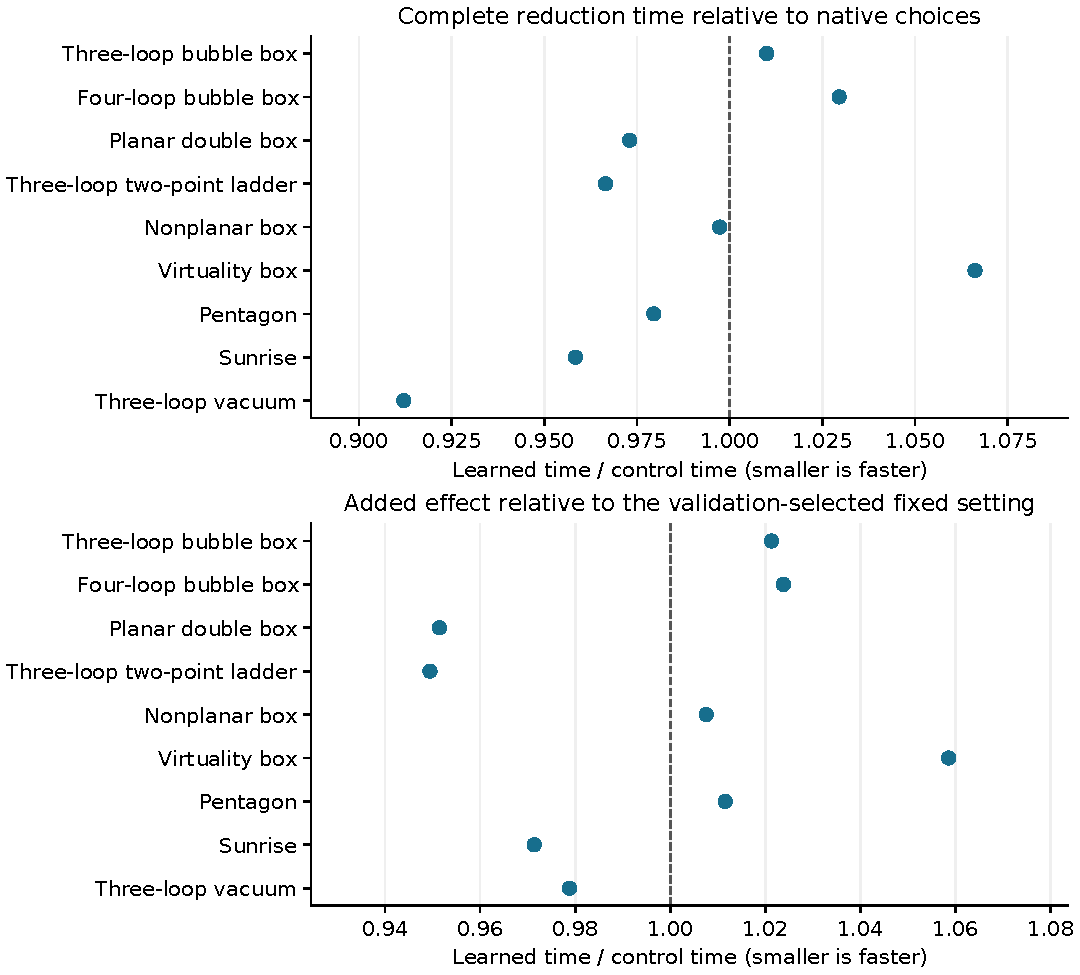
\includegraphics[width=\linewidth]{paper_figures/adaptive_reduction.pdf}
\caption{The upper panel compares the learned policy with native choices after the common exact improvements. The lower panel compares it with the best fixed validation choice. Each point divides sums of batch medians within one graph structure. Values below one indicate less time; the equal-time line remains visible. Three repetitions support descriptive comparisons, rather than a general speed guarantee.}
\label{fig:adaptive}\end{figure}

\subsection{A stronger fixed control and the deployed policy}
One fixed setting for all graphs can be a weak control because different denominator structures can favour different seed regions. We therefore select a separate fixed setting for each graph using validation data only. We also fit 21 small regression trees separately for the graphs with sufficient training cases. They use the same measured cost labels and can specialize in the effect of target powers and numerator rank within one denominator structure. Validation compares these trees with the global model and selects a predictor and gate for each graph. Fitting the additional trees takes 0.723 seconds, with no additional label-generation cost.

We compare the graph-specific fixed settings, the original global model, and a validated policy that uses its selected predictor only where validation supports an additional saving. This procedure was specified before any reserved timings were collected. The final rule requires at least two percent less summed validation time and a saving in both validation repetitions; otherwise the graph's fixed setting is used. All choices remain fixed during the matched comparison. Appendix~\ref{app:adaptive} defines the local models and selection rule.

Validation enables target-dependent predictions for planar double box, three-loop two-point ladder, nonplanar box. Table~\ref{tab:adaptive-graph} gives a separate matched comparison on the same reserved targets, with three repetitions per method. The graph-specific fixed choices take 105.909 seconds, the cost model takes 103.896 seconds, and the validated policy takes 103.983 seconds, using sums of batch medians. The validated policy uses 1.8\% less time than the graph-specific control. Across all repetitions, its time ratio is 0.9830. All 234 reductions pass exact coefficient checks. The fixed choices and validated policy require 21 and 9 recovery attempts, respectively. Figure~\ref{fig:adaptive-graph} shows where predictions add value beyond a fixed choice for each graph.

\begin{table}[!htbp]\centering\small
\caption{Matched complete times in seconds against the stronger fixed control. The validated policy keeps fixed choices where validation does not support the model.}
\label{tab:adaptive-graph}
\begin{tabular}{@{}lrrr@{}}\toprule
Graph & Fixed per graph & Cost model & Validated policy\\\midrule
Three-loop bubble box & 2.197 & 2.190 & 2.201\\
Four-loop bubble box & 28.777 & 29.170 & 28.961\\
Planar double box & 9.932 & 9.275 & 9.333\\
Three-loop two-point ladder & 23.542 & 22.620 & 22.518\\
Nonplanar box & 30.572 & 29.734 & 29.839\\
Virtuality box & 2.207 & 2.160 & 2.213\\
Pentagon & 3.124 & 3.295 & 3.371\\
Sunrise & 1.855 & 1.873 & 1.791\\
Three-loop vacuum & 3.702 & 3.576 & 3.756\\
\midrule Total & 105.909 & 103.896 & 103.983\\\bottomrule
\end{tabular}\end{table}

\begin{figure}[tbp]\centering
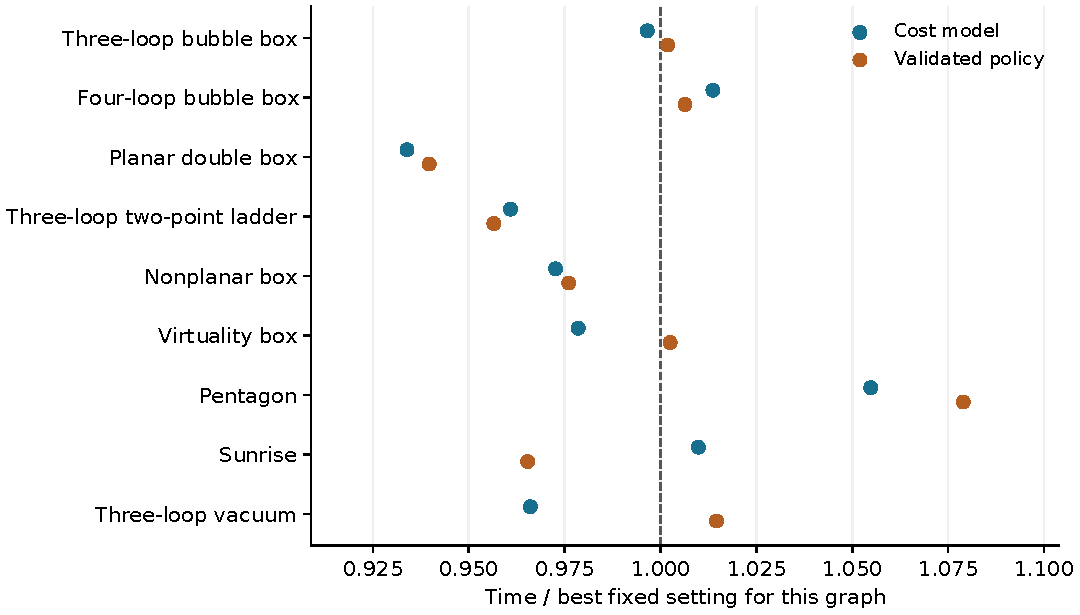
\includegraphics[width=\linewidth]{paper_figures/adaptive_graph_controls.pdf}
\caption{Added effect of target-dependent choices relative to the best fixed validation setting for each graph. Each point divides summed batch medians in the matched comparison. The validated policy uses the model only in the graph structures selected by its validation rule. Timing differences also remain when two methods choose the same setting.}
\label{fig:adaptive-graph}\end{figure}

The public application uses the validated policy and completes the separate exact checks reported above. It keeps native choices for requests outside the recorded family structures and target ranges. An additional application check confirms this fallback for an unsupported graph label. This guard limits the domain in which the learned prediction is used; it does not establish performance on unseen graph structures.

\subsection{Separating preprocessing and prediction}
We repeat the connected three- and four-loop bubble-box calculations with each exact change enabled in turn, followed by the validated policy. Table~\ref{tab:adaptive-integration} reports matched complete times from these separate trials. Every method receives the same 600-second allowance per attempt. The previous-preparation control retains declared-sector initialization and uses native equation choices in the same executable. It disables the two new exact changes. Thus the overall factor includes deterministic preprocessing as well as any subsequent benefit from its selected settings. The final change from projected preparation includes the validated policy and its graph-specific fixed settings; Figure~\ref{fig:adaptive-integration} keeps these contributions separate.

The 4-loop previous control does not complete within its bounded attempts, after 1190.6 seconds of recorded work. Its remaining 2 repetitions are omitted after this failure, while the other pre-specified settings are completed. It receives no median completion time or speedup factor.

\begin{table}[!htbp]\centering\small
\caption{Matched preparation comparison for the connected bubble boxes. Times are medians of three complete reductions, in seconds. The final column divides previous-preparation time by validated-policy time.}
\label{tab:adaptive-integration}
\begin{tabular}{@{}rrrrrr@{}}\toprule
Loops & Previous & File index & Projection & Validated policy & Overall factor\\\midrule
3 & 6.087 & 5.525 & 2.906 & 2.939 & 2.07\\
4 & Incomplete & 98.408 & 28.197 & 28.666 & --\\
\bottomrule\end{tabular}\end{table}

\begin{figure}[tbp]\centering
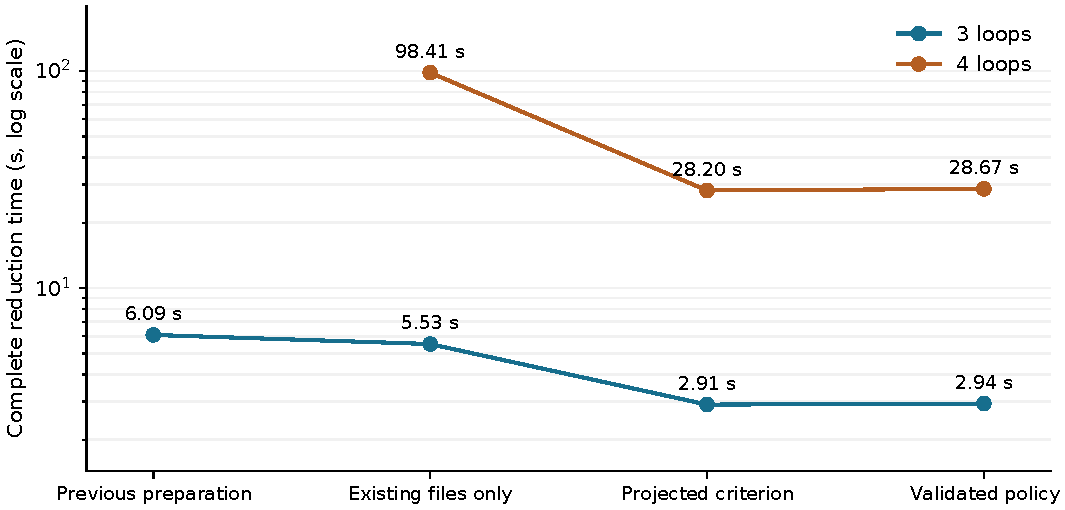
\includegraphics[width=\linewidth]{paper_figures/adaptive_integration.pdf}
\caption{Complete time for the matched preparation study. The logarithmic vertical axis displays the large deterministic change and the final change from the validated policy. The separate graph-specific comparison measures the added effect of prediction. All plotted points represent completed reductions into the same prescribed basis with exact coefficient checks. Incomplete controls are omitted from the curve and reported in the table.}
\label{fig:adaptive-integration}\end{figure}

The new policy makes one inexpensive decision before the costly work begins and retains native row elimination. Its tests cover stated target patterns and kinematics in known families. They do not establish a gain for every integral type, a minimal master basis, or a globally fastest reduction sequence. Reference failures and bounded higher-loop attempts remain part of the evidence. These limits determine where the current measurements support use of the method.

\section{A learned portfolio of complete reduction strategies}
\label{sec:portfolio}
The preceding comparisons show that the useful decision depends on both the denominator structure and the target powers. A seed region that suffices for one batch can leave another batch unreduced, while expanding every seed limit can generate equations that the calculation does not need. We therefore train a model to choose a complete calculation from several strategies before Kira generates the equations. This choice includes the previous workflow as a candidate, so the new policy can retain that workflow when its measured cost is lower.

\subsection{What the model chooses}
For a target batch, let $r_0$ be the largest sum of positive indices, $s_0$ the largest total numerator power, and $d_0$ the largest number of extra denominator powers, or dots. Kira uses limits of this kind to define the seed region~\cite{Kira3}. Our earlier complete-cost policy chooses among seven regions or equation settings, as described in Appendix~\ref{sec:adaptive}. A development comparison reveals a useful additional choice: increase $s_0$ by one while leaving the positive-index and dot limits unchanged. This selective expansion can supply missing identities without the cost of increasing all three limits.

The final portfolio contains five choices: the earlier cost policy with one or two workers, selective numerator-rank expansion with one or two workers, and the previous workflow from Appendix~\ref{app:thread-policy}. A worker carries out tasks in Kira's existing parallel symbolic solver~\cite{KiraOriginal}. The previous workflow combines its existing graph, seed, and worker choices; its parameters remain fixed in this comparison. Each choice uses the same exact preprocessing and a supplied master basis. The three- and four-loop bubble boxes have no trained policy in the previous workflow, so its control uses the documented native fallback. We retain Kira's native row elimination because the learned row model has not reduced complete time reliably.

Each attempt must express every target in the prescribed basis. If it cannot do so, the calculation retries with native seeds and then an expanded seed region. We skip a repeated attempt when its effective seed bounds, ordering, and equation filter are identical to those already tried. The model does not predict reduction coefficients. It predicts the relative time of these complete strategies, including checks, failed attempts, and recovery. Appendix~\ref{app:portfolio} defines the model inputs, objective, guard, and exact recovery procedure.

\subsection{Training and independent tests}
We fit 30 candidate predictors using 47 training batches and select the predictor, fixed control, and decision threshold using 26 separate validation batches. The candidates include regression trees, random forests, and extremely randomized trees~\cite{CART1984,Breiman2001Forest,Geurts2006ExtraTrees}. Their twenty inputs describe the graph structure, target powers, numerator ranks, number of targets, and distribution of dots. They contain no reference coefficients or measured test times. The recorded label calculations take 1858.3 seconds, and fitting takes 2.621 seconds. These costs occur before deployment.

For each graph, validation also selects the fastest fixed portfolio choice. The model replaces this choice only if it reduces summed validation time by at least two percent and gives a saving in both validation repetitions. This rule enables target-dependent portfolio predictions for planar double box, three-loop two-point ladder, nonplanar box, sunrise. All enabled outer predictors are single regression trees. A retained portfolio choice can itself contain an earlier learned policy; therefore the fixed-portfolio control isolates the added outer decision, rather than removing all earlier learned decisions. Requests outside the recorded graph structures and feature ranges use native settings.

The reserved test uses rational kinematic profile $h=306$ and symbolic targets with a dot position absent from the earlier symbolic training and validation sets. The earlier reserved profiles do not enter fitting or selection. The completed comparison contains 26 batches from nine known graph structures through four loops, with one to three targets per batch. Appendix~\ref{app:portfolio} specifies the targets and reference checks. These tests change kinematics and target positions within known structures; some rational target patterns recur across profiles. They do not test transfer to arbitrary new graphs or larger target batches.

Every method receives the same two-core allocation and an 8\,GiB memory allowance. The native control and earlier cost-policy control use one Kira worker. The previous workflow, fixed portfolio, and selected portfolio can use one or two workers according to their chosen strategy. We rotate method order and repeat each method three times, with a fresh Kira process and temporary files for every attempt. Complete time includes prediction, preparation, exact algebra, coefficient checks, cleanup, and recovery. Model imports, initial model loading, reference construction, and basis discovery are separate. No coefficient cache supplies the test answers.

\subsection{Complete-time results}
Table~\ref{tab:portfolio} sums the three-run median times of the individual batches. The selected portfolio takes 85.497 seconds, compared with 108.029 seconds for native choices and 95.382 seconds for the previous workflow in the same improved executable. These results correspond to 20.9\% less time than native choices and 10.4\% less time than the previous workflow. The earlier cost policy takes 102.561 seconds on these same inputs. The graph-specific fixed portfolio takes 86.809 seconds, so the added portfolio decision gives 1.5\% less time relative to this stronger control. Figure~\ref{fig:portfolio-controls} shows where these differences occur.

Summing every timed repetition gives 19.4\% less time than native choices, 9.4\% less time than the previous workflow, and 0.4\% more time than the fixed portfolio. The small difference from the fixed portfolio changes sign between the two summaries. These measurements establish no stable aggregate saving from the added outer prediction. The practical improvement over the previous workflow includes the revised candidate strategies and worker choices, which also benefit the fixed portfolio.

\begin{table}[!htbp]\centering\small
\caption{Complete reduction times in seconds. Each row sums batch medians from matched tests with common exact preprocessing. ``Fixed'' selects a portfolio choice per graph using validation only.}
\label{tab:portfolio}
\begin{tabular}{@{}lrrrr@{}}\toprule
Graph & Native & Previous & Fixed & Selected\\\midrule
Three-loop bubble box & 2.280 & 2.300 & 2.274 & 2.388\\
Four-loop bubble box & 32.420 & 29.726 & 28.981 & 29.129\\
Planar double box & 9.478 & 8.226 & 8.179 & 7.406\\
Three-loop two-point ladder & 23.326 & 17.584 & 14.314 & 14.108\\
Nonplanar box & 28.380 & 25.414 & 20.793 & 20.236\\
Virtuality box & 2.585 & 2.756 & 2.763 & 2.608\\
Pentagon & 3.895 & 3.922 & 4.072 & 3.966\\
Sunrise & 1.941 & 1.677 & 1.661 & 1.770\\
Three-loop vacuum & 3.724 & 3.777 & 3.772 & 3.886\\
\midrule Total & 108.029 & 95.382 & 86.809 & 85.497\\\bottomrule
\end{tabular}\end{table}

All 390 timed reductions and 26 further applications reproduce the reference coefficients exactly. The applications receive only the prescribed master basis before reduction; the comparison with reference coefficients follows execution. The selected portfolio requires 3 recovery attempts across the timed tests. Its median outer decision time is 0.575 milliseconds. The CPU-time totals are 115.370 seconds for native choices and 114.666 seconds for the selected portfolio. Reporting both wall and CPU time separates elapsed-time savings from changes in CPU use, as shown in Figure~\ref{fig:portfolio-totals}. Every planned batch completes both reference calculations.

The dotted three-loop two-point ladder illustrates the change in the equation system. Native choices use seed limits $(10,0,2)$, then $(11,1,3)$, while the selected portfolio uses $(10,1,2)$, in the order $(r,s,d_{\rm dots})$. Summing the reported generated-equation counts across all attempts gives medians of 287,558 equations for native choices and 94,380 for the selected portfolio. Their complete times are 14.637 and 7.345 seconds. This count measures equation generation; symbolic simplification can require different work per equation. The CPU-time comparison also accounts for the effect of worker count.

The application also avoids loading the previous workflow until a selected strategy requires it. On the dotted sunrise batch, three rotated comparisons of a new application instance give median request times of 3.258 seconds with immediate loading and 0.727 seconds with deferred loading. These times include construction, one reduction, an exact coefficient check, and closure, while common Python imports remain outside the timer. All six requests choose the same strategy and return the same exact coefficients. This separate interface saving applies when the request does not need the previous workflow. A request that first selects that workflow pays its loading cost within the application time. The repeated portfolio timings above already keep the models loaded, so they receive no additional saving from this change.

\begin{figure}[tbp]\centering
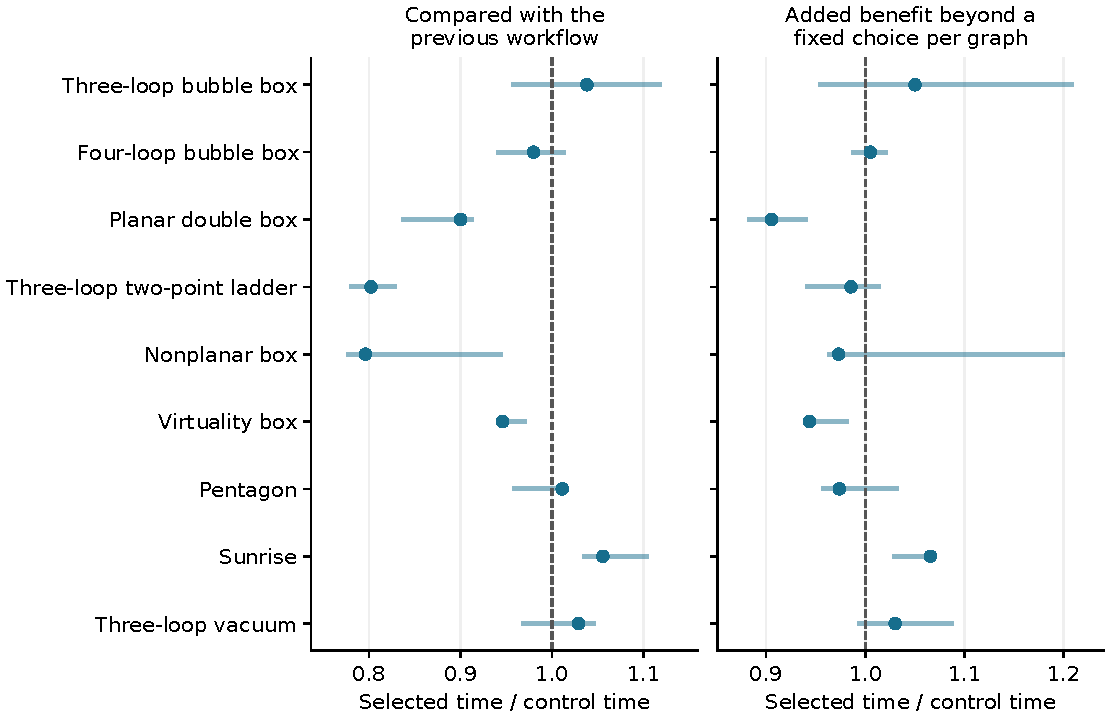
\includegraphics[width=\linewidth]{paper_figures/portfolio_controls.pdf}
\caption{Selected-portfolio time relative to the previous workflow and the graph-specific fixed portfolio. Points divide sums of batch median times. Horizontal segments show the range of the three corresponding repetition totals; they are descriptive ranges, not confidence intervals. Values below one indicate a saving.}
\label{fig:portfolio-controls}\end{figure}

\begin{figure}[tbp]\centering
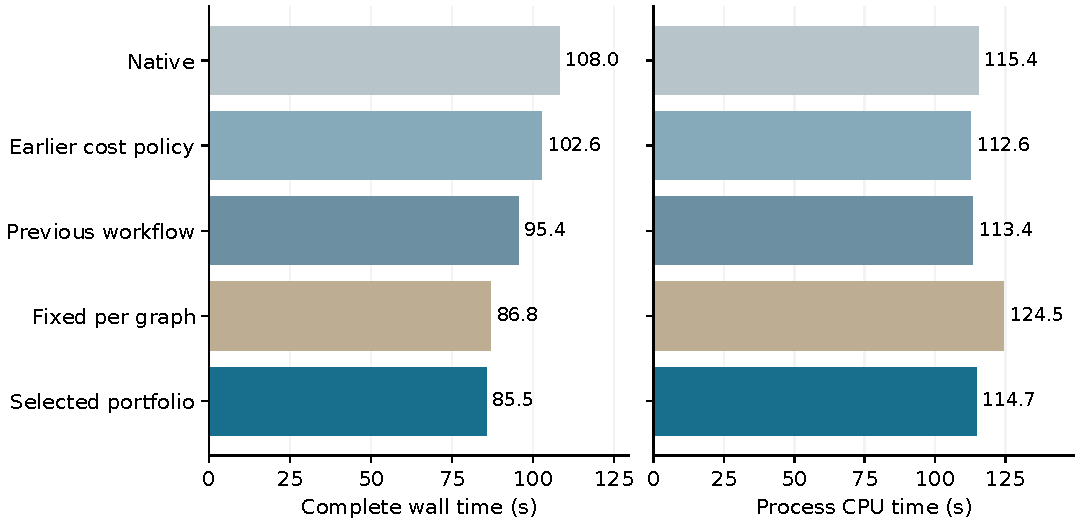
\includegraphics[width=\linewidth]{paper_figures/portfolio_totals.pdf}
\caption{Complete wall time and recorded process CPU time for the same reserved batches. The five methods share exact preprocessing and a two-core allocation. CPU time counts the main driver, Kira child processes, and the timed part of the previous-workflow service. Its message conversion lies outside that service's CPU counter but remains in complete wall time. Initial loading lies outside the repeated timings.}
\label{fig:portfolio-totals}\end{figure}

\subsection{Separating the exact implementation changes}
The portfolio tests use two exact improvements in every method. We index the sector files that exist instead of searching for absent files, while retaining their original processing order. We also simplify the criterion for zero sectors by setting Feynman parameters absent from all declared top sectors to zero before forming that criterion. The complete parametric polynomials remain available for the other operations. Appendix~\ref{app:adaptive} proves why this projection preserves the criterion in the declared sector domain, following the parametric treatment of zero sectors~\cite{Lee2014LiteRed}.

Separate matched tests enable these changes in sequence for connected bubble boxes. For the 3-loop batch, the complete time changes from 6.087 to 2.939 seconds with the first study's validated policy, an overall factor of 2.07. The 4-loop previous-preparation control does not complete after 1190.6 seconds across its bounded attempts. Further repetitions of this failed control are omitted, while the remaining settings are completed. The fully improved calculation takes 28.666 seconds, but the incomplete control supplies no measured overall speedup factor. With file indexing already enabled, projection changes its complete time from 98.408 to 28.197 seconds, a factor of 3.49. These comparisons include exact implementation changes and therefore do not measure an isolated ML gain. Figure~\ref{fig:adaptive-integration} and Table~\ref{tab:adaptive-integration} preserve the intermediate controls in the earlier cost study. The common-preprocessing comparison in Table~\ref{tab:portfolio} measures the subsequent portfolio choices separately.

The measurements support the selected strategies in the stated domain. Timing differences can remain when two methods choose the same strategy, and the three repetitions do not establish a significant gain for every graph. General higher-loop scattering, arbitrary symbolic kinematics, automatic discovery of a minimal master basis, and globally optimal elimination paths remain outside the demonstrated scope.

\section{Reducing preparation around the learned choices}
\label{sec:parametric}
The previous comparison leaves a substantial cost even after the model has chosen a useful seed region. On a four-loop development batch, the actual row operations take a small fraction of the total time, while sector symmetry preparation and repeated equation generation dominate. We therefore retain the trained policies and change the exact work that surrounds their choices. This comparison tests whether better integration can make the same predictions more useful without adding another model or changing its weights.

\subsection{Avoiding unused polynomial terms and repeated equations}
Kira uses parametric polynomials to identify zero sectors and sector symmetries~\cite{KiraOriginal,Lee2014LiteRed}. Each inverse propagator has a Schwinger parameter, an auxiliary variable in this representation. An auxiliary inverse propagator can occur in a numerator while its index remains nonpositive throughout the declared sector domain. Its Schwinger parameter then vanishes in the sector polynomials used for these checks. The preceding implementation first constructs the full polynomials and removes the unused parameter terms from the zero-sector criterion. We now apply this substitution before polynomial construction and use the resulting restricted polynomials for both zero-sector and symmetry checks. Appendix~\ref{app:parametric} proves that this change gives the same polynomial in every admitted sector. The full propagator list remains available when Kira forms IBP identities and transforms numerators.

Kira also constructs selected symbolic equations to check their remaining masters, then constructs those equations again for the final reduction. We keep the unmodified exact rows from the first construction. When the next selection returns the identical ordered list of source equations, the calculation uses those saved rows. If the selection changes or the storage allowance is exceeded, Kira regenerates the equations normally. The saved rows exist only within that reduction; no previous target answer supplies a later result. This change removes a repeated calculation of an established identity. It does not replace equation selection or symbolic elimination.

The application uses the same trained portfolio, graph-specific predictors, thresholds, seed settings, worker choices, and recovery rules as Section~\ref{sec:portfolio}. We fit no model in this comparison. Thus any change relative to the previous application measures the exact integration changes and timing variation. A matched fixed-portfolio control measures the additional effect of the outer prediction. The earlier separate service remains available for the few requests assigned to it, and its full cost remains in the measurement.

\subsection{Fresh targets and matched controls}
We reserve 26 new batches from the same nine graph structures, with one to three targets per batch and loop orders one through four. The rational cases use a fresh parameter profile. The symbolic nonplanar and pentagon cases move the raised denominator power to a new position, while the virtuality box has two singly dotted denominators. Appendix~\ref{app:parametric} specifies these inputs. The frozen range guard can select native settings when a new target pattern lies outside its training range.

The first reference reduction uses expanded seeds with the revised preparation. A second calculation uses the previous executable and a larger numerator-rank limit to check the resulting coefficients in the same basis. Each timed method then receives the target and that prescribed basis. Reference coefficients enter only the comparison after the calculation. The test checks reduction to this basis, rather than proving that the basis is minimal.

We compare four methods: the previous application; native choices with revised preparation; a graph-specific fixed portfolio with revised preparation; and the selected portfolio with revised preparation. The fixed portfolio can contain an earlier learned policy, so it isolates the added outer choice. All methods use the same two-core allocation, memory limits, and exact checks. Native choices use one Kira worker, while the portfolios retain their chosen one or two workers. The revised controls share the application's input checks and portfolio proposal; the native and fixed controls then override that proposal. We report the effect of removing this common overhead below. Each attempt starts a fresh Kira process with fresh temporary files. Three repetitions rotate method order. Complete time includes decisions, input preparation, algebra, coefficient checks, cleanup, and unsuccessful attempts. Initial model loading, reference construction, and basis discovery remain outside these repeated timings.

\subsection{Results and attribution}
Table~\ref{tab:parametric} sums the median time of each batch. The revised selected application takes 64.183 seconds, compared with 79.784 seconds for the previous application. This is 19.6\% less time on the measured collection. The selected actions agree with the previous application for every batch and repetition, so this improvement comes from the exact preparation changes around the existing models. Summing all repetitions gives 19.6\% less time than the previous application.

\begin{table}[!htbp]\centering\small
\caption{Complete times in seconds, summed over batch medians. The previous column uses the earlier preparation. The other columns enable both exact changes for direct Kira attempts; the earlier separate service retains its preparation. Fixed denotes the validation-selected portfolio choice for each graph.}
\label{tab:parametric}
\begin{tabular}{@{}lrrrr@{}}\toprule
Graph & Previous & Native & Fixed & Selected\\\midrule
Sunrise (2 loops) & 1.742 & 1.706 & 1.806 & 1.793\\
Planar double box (2) & 6.155 & 8.501 & 7.123 & 5.953\\
Vacuum (3) & 2.788 & 2.678 & 2.678 & 2.636\\
Two-point ladder (3) & 13.393 & 23.400 & 12.917 & 11.581\\
Nonplanar box (2) & 19.794 & 28.662 & 20.478 & 20.052\\
Pentagon (1) & 3.094 & 2.989 & 3.003 & 3.022\\
Virtuality box (1) & 2.172 & 2.216 & 2.232 & 2.229\\
Bubble box (3) & 2.225 & 1.617 & 1.735 & 1.647\\
Bubble box (4) & 28.421 & 16.078 & 15.409 & 15.271\\
\midrule Total & 79.784 & 87.847 & 67.381 & 64.183\\\bottomrule
\end{tabular}\end{table}

With each candidate implemented in the same way for all controls, the selected method uses 26.9\% less time than native choices and 4.7\% less time than the fixed portfolio. Across all repetitions, its difference from the fixed portfolio is 5.0\% less time. These controls keep the effect of learned decisions separate from exact reuse. The graph results in Figure~\ref{fig:parametric} show the measured savings and regressions; a smaller total does not imply that every batch becomes faster.

The common interval for input checks and the outer proposal is at most 2.854 milliseconds per revised request. Removing this entire measured interval from the native and fixed controls gives optimistic totals of 87.828 and 67.363 seconds, respectively. The selected method then uses 4.7\% less time than this optimistic fixed control. This subtraction removes useful checks as well as the unused proposal and therefore serves as a sensitivity bound, rather than a separately timed implementation.

All 312 timed reductions and 26 further basis-only applications reproduce their checked reference coefficients exactly. The reference checks, timed tests, and applications compare 8,086 target--master coefficients. The revised selected method needs 6 recovery attempts across its timed tests. The recorded process-tree memory peak among the timed reductions is 961.8 MiB. The selected method takes 92.782 seconds in summed batch median CPU time, compared with 107.054 seconds for the previous application. The bounded replay mechanism activates 117 times across the timed controls and retains at most 0.221 MiB of accounted row data in an activation.

\begin{figure}[tbp]\centering
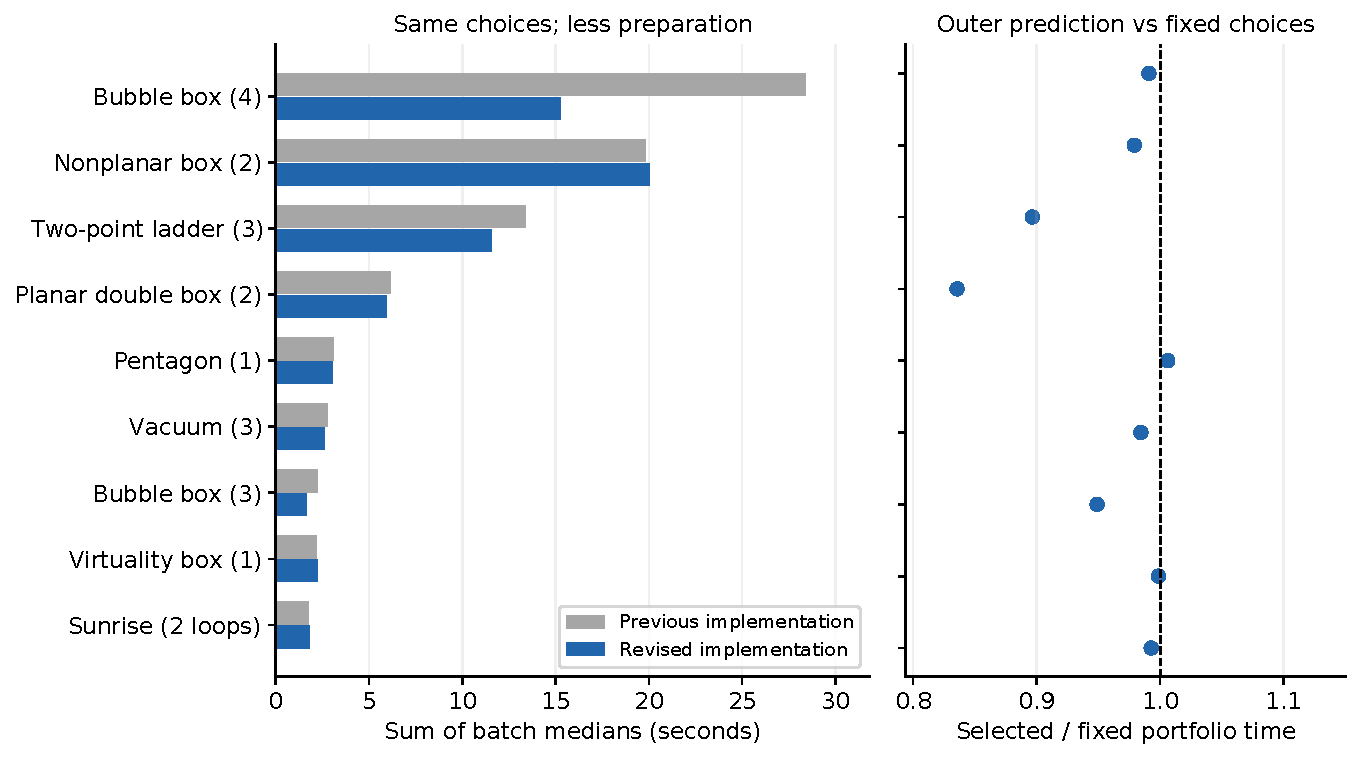
\includegraphics[width=\linewidth]{paper_figures/parametric_results.pdf}
\caption{Left: the same learned actions run with the previous and revised preparation. Right: the selected-to-fixed time ratio with revised preparation; the dashed line marks equal time. Each point or bar uses sums of batch medians within a graph. The right panel isolates the additional outer prediction.}
\label{fig:parametric}
\end{figure}

These results support the revised application for this measured collection. They test new parameters and target patterns within known graph structures, with supplied master bases. They do not establish general high-loop scattering performance or a globally shortest reduction. The earlier row-model result remains unchanged, so the application continues to use native row elimination.

\newcommand{\CoverageVacuumDerivation}{Section~\ref{sec:higher-loop-generation}}
\providecommand{\CoverageVacuumDerivation}{Appendix~\ref{app:vacuum}}
\section{How far the improvement extends}
\label{sec:coverage}
The preceding gain was measured on known graph structures with a supplied master basis. To test its wider use, we now vary the physical structure as well as the loop order and include calculations that find their own basis. We keep the deployed models fixed so that these measurements test the current method on new inputs. The study contains 90 native-family requests, of which 54 fit the application's current index limit. It also tests a separate restricted vacuum construction at every loop order from one through twelve. This is a finite coverage study; a loop-order label alone does not establish coverage of all graphs at that order.

\subsection{Physical families and complete-time controls}
The native grid includes vacuum families with one or several masses, massless and massive two-point families, four-point ladders, and boxes with bubble subgraphs. We add planar, nonplanar, and five-point examples with independent symbolic kinematic parameters. Appendix~\ref{app:coverage} gives the denominator definitions, parameters, and targets. The 82 initial requests contain a sector-corner integral, one raised propagator power, and one numerator integral when an auxiliary denominator is available. Some massive two-point batches return every target unchanged as a master. We therefore preserve those results and add 8 separate batches containing every distribution of up to two dots over the physical denominators. The additional batches cover all six loop orders accepted for that two-point family, plus symbolic cases at one and two loops. Their inputs are fixed before their own comparison, and no model is refitted from either stage.

We first calculate a reference with expanded seeds and the revised implementation. A second calculation uses the previous executable and a larger numerator-rank bound, with the reference basis prescribed. Both must complete and reproduce the same coefficients before a case enters the repeated comparisons. This checks the reductions in the stated basis; it does not prove that the basis has the smallest possible size. Every native attempt has a 120-second allowance, a 6 GiB address-space limit, and a 5,200 MiB process-tree memory limit. An attempt that reaches a limit remains a failed result. Inputs with more than 31 indices exceed the current application's accepted domain and receive no timing estimate.

The first comparison runs the saved original Kira executable, the previous improved implementation, and the revised implementation with the same expanded seed region. These calculations receive no master list, so their times include basis discovery, equation generation, elimination, coefficient checks, and cleanup. This comparison measures the complete effect of the implementation. It makes no learned decision. The second comparison supplies the checked basis and runs the previous learned application, the revised learned application, and a native-choice control with revised preparation. Its times also include prediction and unsuccessful attempts. Both comparisons use three repetitions with rotated method order and fresh Kira processes. Initial caller imports and model loading remain separate from the repeated application times.

An input audit finds two box-with-bubble definitions that match saved training structures exactly but carry new family names. The initial application treats these names as unknown. We add a lookup that resolves a unique match of the ordered momentum forms, sector definition, and zero or nonzero mass pattern before prediction. Numerical mass and kinematic values remain free, as in the existing model signature, and all original feature-range checks remain active. Unmatched structures retain the native fallback. The lookup uses no measured time or reference coefficient. We repeat the paired application comparison for both names and use these corrected pairs in the application totals. The initial unknown-name measurements remain available separately. This correction allows the existing models to recognize their own domain; it does not train a new model or infer equivalence between different momentum representations.

\subsection{Coverage and measured time}
Figure~\ref{fig:coverage-grid} shows the rational grid, including its failures and unsupported inputs. The reference checks pass for 41 requests, and 41 requests complete all three revised full-calculation repetitions. Of these, 39 contain a nontrivial reduction and 2 contain only identity outputs. We exclude identity-only requests from speedup ratios. The supplied-basis selected application completes all repetitions for 41 requests. The remaining requests retain their stated failure or support-limit classification. The timings therefore do not establish a nontrivial reduction for every entry in the grid.

\begin{figure}[!htbp]\centering
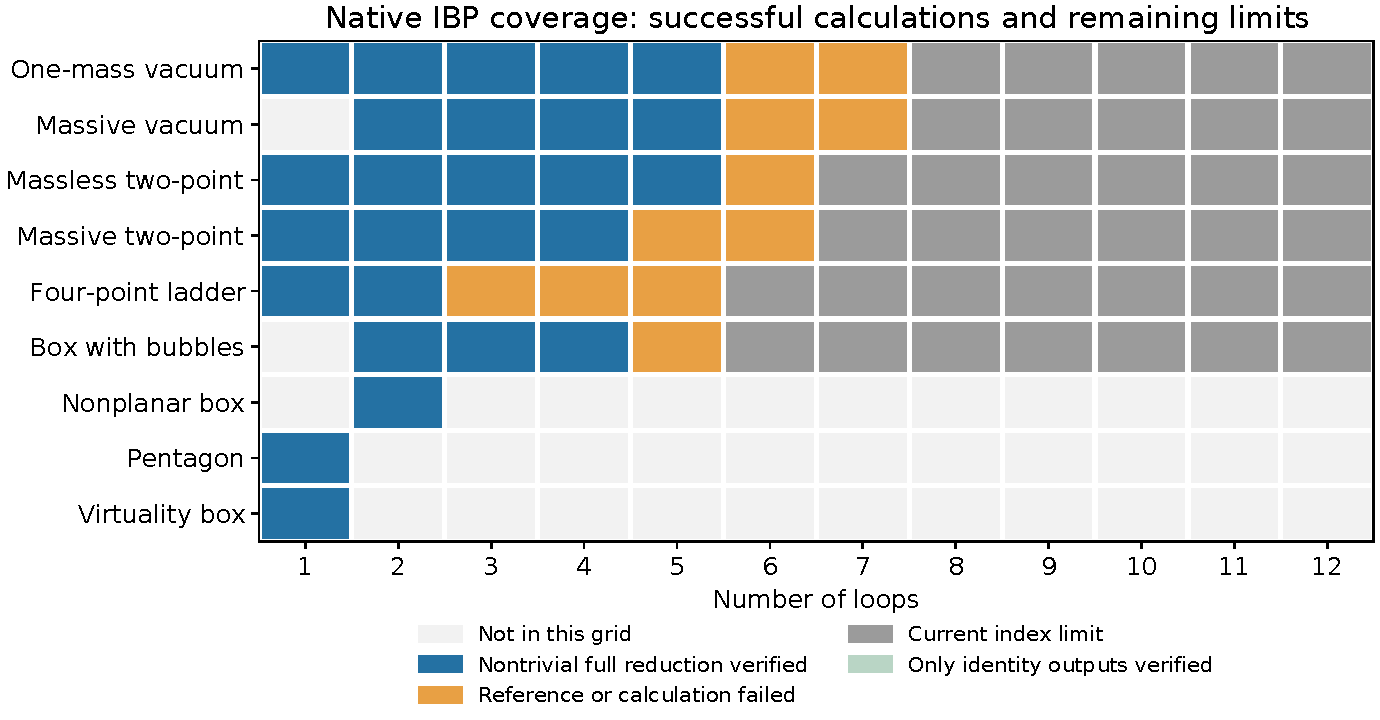
\includegraphics[width=\linewidth]{paper_figures/coverage_grid.pdf}
\caption{Native IBP coverage in the rational grid. Blue requires a checked reference, a nontrivial reduction, and three exact revised full calculations including basis discovery. Pale green records only identity outputs. Orange records a failed reference or calculation within the stated limits. Gray records the current index limit. A cell takes the strongest verified status across initial and additional batches. Blank cells are absent from this grid; the two coincident one-loop definitions appear only once. Symbolic requests enter the timing table and the text totals.}
\label{fig:coverage-grid}
\end{figure}

Table~\ref{tab:coverage-times} uses a separate matched set for each comparison. A request enters a row only when both methods complete all repetitions and the reduction contains a nontrivial coefficient. We sum the median time of each request, so a smaller ratio means less total time on that completed set. The revised full calculation takes 88.2\% less time than the saved original Kira executable and 54.3\% less time than the preceding improved implementation on their respective matched sets. The supplied-basis selected application takes 54.1\% less time than the previous application and 0.1\% less time than the revised native control. These aggregates retain slower individual requests and do not turn unsuccessful cases into speedup estimates.

\begin{table}[!htbp]\centering\small
\caption{Summed request median times in seconds. The revised column uses full revised calculations for the first two rows and the selected application for the last two. Each row names its own control and completed request count.}
\label{tab:coverage-times}
\begin{tabular}{@{}lrrrr@{}}\toprule
Control & Requests & Control time & Revised time & Ratio\\\midrule
Full: original Kira & 37 & 369.363 & 43.750 & 0.118\\
Full: previous implementation & 39 & 146.541 & 66.897 & 0.457\\
Basis supplied: previous application & 39 & 146.342 & 67.195 & 0.459\\
Basis supplied: revised native control & 39 & 67.269 & 67.195 & 0.999\\
\bottomrule\end{tabular}
\end{table}

The revised native control passes through the same input checks and portfolio proposal before overriding the proposed action. For a conservative comparison, we subtract that entire recorded interval and the family-name lookup from its time, while retaining every selected-application cost. The largest removed interval is 2.124 milliseconds. This gives an optimistic native total of 67.259 seconds, against which the selected application takes 0.1\% less time. The subtraction also removes useful input checks, so it supplies a sensitivity bound rather than a separately timed implementation.

The selected application and revised native control differ by only 0.1\% in the summed medians. With only three repetitions, this small difference does not establish a reliable additional learned gain on the wider grid. The larger improvement against the preceding application includes the exact preparation changes.

The repeated native comparisons contain 752 recorded requests, with 750 exact completions and 2 unsuccessful requests. The largest recorded process-tree memory use among these timings is 961.8 MiB. The grid includes new graph definitions, so the existing domain guard often retains native choices. This is part of the deployed method and prevents us from describing the full implementation gain as a gain from newly learned decisions.

Table~\ref{tab:coverage-completion} also includes unsuccessful first timed requests. Its elapsed totals describe the cost actually incurred on that common reference-verified collection. They are not completed-reduction speedups, since a failed request supplies no accepted answer. This view complements the paired timing table and prevents completion failures from disappearing in an aggregate improvement claim.
\begin{table}[!htbp]\centering\small
\caption{First timed requests on the reference-verified collection. Elapsed seconds include failed requests. Later repetitions are excluded from this table so that each method receives one request per case.}
\label{tab:coverage-completion}
\begin{tabular}{@{}lrrr@{}}\toprule
Method & Requested & Exact completions & Elapsed seconds\\\midrule
Full original Kira & 41 & 39 & 623.836\\
Full previous implementation & 41 & 41 & 148.606\\
Full revised implementation & 41 & 41 & 68.568\\
Previous application & 41 & 41 & 150.733\\
Selected application & 41 & 41 & 68.497\\
Revised native control & 41 & 41 & 68.721\\
\bottomrule\end{tabular}
\end{table}

\subsection{Every tested loop order in the restricted vacuum class}
The existing vacuum recurrence has a different domain: unit powers on the massless lines and several massive denominators with the same total loop momentum. We construct three new mass profiles with two, three, or four distinct masses and six target exponent vectors per profile. We compare the saved original Kira, dense and selected supplied-identity systems, the frozen learned identity selector, and the deployed exact recurrence. Each method receives the same targets and passes the independent coefficient check derived in \CoverageVacuumDerivation{}. The individual requests cover every loop order from one through twelve. Separate shared requests ask for all twelve orders together.

The study records 585 exact completions in 585 vacuum requests. Table~\ref{tab:coverage-vacuum} separates individual-loop requests from shared requests. In the individual-loop set, learned identity selection takes 8.2\% more time than the fixed identity rule. The deployed recurrence takes 99.8\% less time than the saved original Kira calculation. This gain uses the exact restricted-family relations and their implementation; the deployed recurrence uses its existing fixed policy. The native study and this supplied-identity study therefore establish different forms of coverage.

\begin{table}[!htbp]\centering\small
\caption{Restricted vacuum timings in seconds, summed over request medians. There are 36 individual-loop requests and three shared requests, each repeated three times. The original control solves separately for each requested loop order. The other methods can use the exact shared variable $z=L(d-2)$. All times include coefficient verification.}
\label{tab:coverage-vacuum}
\begin{tabular}{@{}lrr@{}}\toprule
Method & Individual loops & Shared loops\\\midrule
Original Kira, separate loop orders & 122.179 & 129.306\\
Improved Kira, dense identities & 14.626 & 1.310\\
Fixed identity selection & 13.311 & 1.398\\
Learned identity selection & 14.399 & 1.327\\
Deployed exact recurrence & 0.189 & 0.069\\
\bottomrule\end{tabular}
\end{table}

\begin{figure}[!htbp]\centering
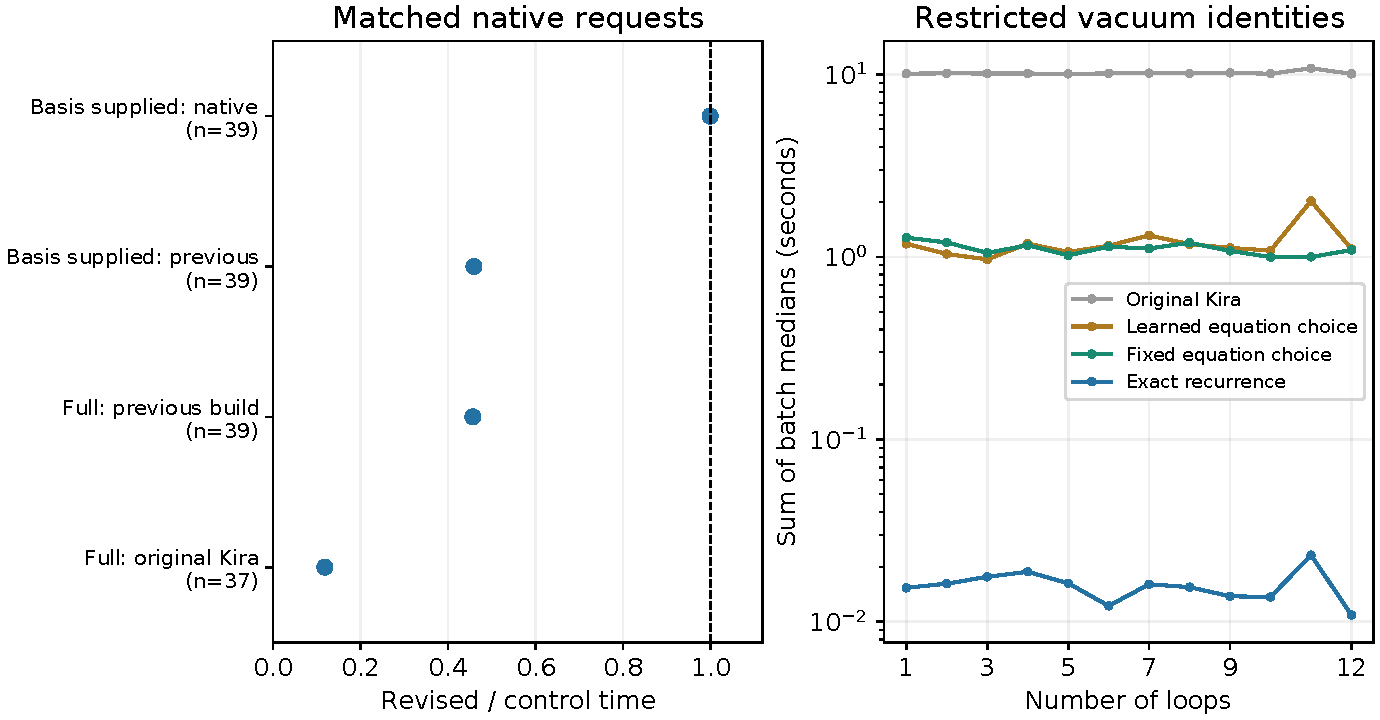
\includegraphics[width=\linewidth]{paper_figures/coverage_times.pdf}
\caption{Left: revised-to-control time ratios on matched completed native requests; the dashed line marks equal time. The request count changes with each pair's completed coverage. Right: restricted vacuum time at each loop order, summed over the three mass profiles. The logarithmic vertical axis keeps the exact recurrence and Kira-based calculations visible. These panels use different integral definitions and cannot be combined into a universal speedup.}
\label{fig:coverage-times}
\end{figure}

The broader tests identify where the current application completes an exact reduction, where its cost changes, and where its support or resource limits stop the calculation. They retain the earlier known-graph gain while restricting its interpretation to measured inputs. General high-loop scattering, arbitrary numerator rank, cuts, symbolic propagator powers, and every possible mass or kinematic assignment remain outside a universal verified claim.


% END CURRENT WORKFLOW UPDATE
\section{Conclusion}
\label{sec:conclusion}
We integrated seed and source-row policies with exact native Kira reduction
and reduced their evaluation cost while retaining the same decisions.
The latest seed implementation evaluates independent neural outputs together,
and the row implementation combines Euclid's modular inverse with direct
integer evaluation and shared coefficient storage.
All probability vectors agree in the thirty-six development contexts.
Checks on 100,000 inverses and 1,000 sparse-row groups also agree.

The new seed component has a time ratio of 0.423 to the preceding shared implementation. The row-feature component has a ratio of 0.803. These component savings require separate complete-reduction measurements because model evaluation is only one part of the calculation.

The seed method has a complete-time ratio of 0.990 to its preceding implementation, with descriptive interval $[0.977,1.003]$. Its ratio to the new native control is 1.096, with interval $[0.963,1.275]$.

The row method has a complete-time ratio of 0.990 to its preceding implementation, with descriptive interval $[0.971,1.010]$. Its ratio to the new native control is 0.982, with interval $[0.959,1.003]$.

The combined method has a complete-time ratio of 0.984 to its preceding implementation, with descriptive interval $[0.965,1.007]$. Its ratio to the new native control is 1.100, with interval $[0.966,1.279]$.

The descriptive complete-time intervals include one for all three comparisons with the preceding implementation. Component evaluation is faster, and the complete-workflow gain remains uncertain at this sample size. The seed and combined methods still have aggregate costs above the native control. The row-only comparison with native choices also includes one in its interval.

All 144 validation workflows and 640 confirmation workflows pass the exact
checks and preserve the recorded decisions and operation counts. These times
include IBP generation, model evaluation, exact algebra, checks and fallback.
The implementation comparison reuses eight physical
profiles and retains the weights, thresholds and routing selected before
confirmation~\cite{KiraParallelInferenceData}.


The data construction provides 17,100 family instances, 57,979 family-local
master entries and 2,301,272 targets with recorded identities and reduction
paths. These paths provide valid reference constructions and costs.
On 690,382 held-out targets, the seed model reaches 96.318\% $F_1$, and its
predicted stored equations supply complete master-span reductions for
94.515\% of targets. The full candidate pool supplies the remaining reductions.
These label and sufficiency measures require separate runtime tests; the
earlier cost comparisons and their negative results remain part of the
study~\cite{HigherLoopIntegralData,SeedModelTestData,KiraSeedSufficiencyData,KiraCostComparisonData}.

For production use, the interface needs a prescribed master basis and can
calculate target coefficients without their reference answers. Native exact
IBP operations determine the coefficients, and explicit output-basis admission
detects incomplete seed sets. Eight application checks pass independent
coefficient comparisons after execution with reference answers withheld
from the reducer. The report keeps this native algebraic assurance separate
from the additional reference comparisons used in the benchmark.

The original collection through twelve loops uses restricted coupled vacuum
families. The native performance comparisons cover physical two- and
three-loop inputs at fixed rational kinematics with symbolic $d$.
The ladder topology is absent from that row-policy training and validation
sets. Those native timing comparisons retain their fixed-kinematic scope.
Section~\ref{sec:generalization} extends the tests to new scattering
topologies and independent symbolic invariants and supplies finite
optimality certificates. General high-loop scattering and optimality
over unrestricted identity pools remain open.







% BEGIN EQUATION CONCLUSION
The third model selects generated identities for the requested targets.
The broad test found that incomplete vacuum filters added fallback cost.
A restricted route was then fixed and tested on six fresh sunrise profiles.
It gives a complete-time ratio of 0.994, with descriptive interval $[0.991,0.997]$
and an equation-preparation ratio of 0.785, with descriptive interval $[0.776,0.794]$.
All 162 confirmation comparisons, 36 checks with the two earlier models
and six applications pass exact coefficient checks. The preceding deployed equation
policy uses the recorded 21-target sunrise domain and retains native
choices elsewhere~\cite{KiraEquationSelectionData}.
The measured three-model composition is slower, with time ratio 1.317 to the earlier two-model configuration. That preceding interface therefore retains native equation choices when either earlier learned policy is active.
% END EQUATION CONCLUSION


% BEGIN EARLY EQUATION CONCLUSION
Later training moves the equation decision before coefficient construction.
The trees use 17 seed, operator and target features and train on
153,124 native candidates in eight physical profiles.
Validation selects early filtering with native seed and row choices for
the recorded double-box, vacuum and ladder batches and retains the earlier
sunrise route. On eight fresh profiles, the deployed policy gives a
complete-time ratio of 0.943 to native choices, with descriptive interval
$[0.915,0.970]$, and a preparation ratio of 0.638, with interval
$[0.546,0.734]$. Its complete-time ratio to the preceding release is
0.943. All 280 comparisons and eight basis-only applications pass
independent exact checks. These results include inference and fallback costs
and support the measured fixed-kinematic domain. The validation comparisons
with the seed and row models remain recorded, and their added costs keep
those combinations out of the selected route~\cite{KiraEarlyEquationData}.
% END EARLY EQUATION CONCLUSION

% BEGIN HIGHER LOOP CONCLUSION
The higher-loop extension uses the exact variable \(z=L(d-2)\) for the
restricted coupled vacuum family. The trained equation selector and a
shared symbolic reduction cover every tested order from one through
twelve, with exact applications at 13, 16, 24 and 32.
The learned route with separate reductions at each loop order has complete-time ratio
0.911 to the supplied full pool. Validation selects a
simple rule for the mass pair for deployment; its shared route has complete-time
ratio 0.155 to separate reductions with the full equation pool.
Before Python startup and test-record archiving, the learned calculation
has time ratio 0.943; time inside Kira has ratio
0.965. All 96 workflows pass exact checks. These results establish the stated
coefficient reuse within this family and cost comparisons. General
native IBP generation at higher loop orders remains outside this test domain
\cite{KiraHigherLoopData}.
% END HIGHER LOOP CONCLUSION

% BEGIN BATCH REUSE CONCLUSION
The next extension learns shared equation choices for entire target batches
and reduces repeated exact checks in the common variable \(z\). Its
four-tree cost model trains on 420 batches and 6,300 candidate orderings.
Combining independent profiles in one Kira call preserves separate master
bases and reduces repeated startup work. On the final twelve reserved
profiles, the selected combined route has complete-time ratio 0.220
to the preceding separate workflow, with descriptive interval
\([0.171,0.270]\). All 460 reserved applications and the additional
integration checks pass exact comparisons; the integration tests also
verify the full-system fallback. Compiled and Python inference produce
identical equation systems. The comparisons separate model decisions,
shared exact arithmetic and shared Kira calls, and apply to the stated
restricted vacuum family~\cite{KiraBatchReuseData}.
% END BATCH REUSE CONCLUSION

% BEGIN PRE REDUCTION CONCLUSION
The direct-reduction extension evaluates selected triangular identities with exact
integer polynomial arithmetic and checks every master coefficient through
an independent Taylor construction. Validation selects the simple direct route.
On eight fresh three-profile batches, its calculation-time ratio to the
preceding combined workflow is 0.306, with descriptive interval
\([0.246,0.373]\). The full worker-time ratio is 0.430.
All 200 reserved calculations pass exact checks, and an injected failure
recovers through Kira. The comparison does not establish a further complete-time advantage from learned ordering over both direct controls.
The direct saving follows mainly from the exact family-specific recurrence;
the native IBP-generation results retain their earlier scope
\cite{KiraPreReductionData}.
% END PRE REDUCTION CONCLUSION

% BEGIN POLYNOMIAL REUSE CONCLUSION
The polynomial-reuse extension shares the exact transformations for \(z=L(d-2)\)
and the Taylor terms in the independent check. On eight new reserved
batches, both changes together have calculation-time ratio 0.372 to
the preceding direct route and full worker-time ratio 0.682.
Keeping one process for several batches gives combined full-time ratio
0.365 across the three specified request streams. These streams share
inputs, so this last ratio describes those sequences.
All 352 reserved applications pass exact checks, including an independent
audit of 28860 expanded coefficient positions. The request-interface
checks also pass, including recovery through Kira after an injected failure.
The changes reuse exact mathematical work and process startup; the
previous model and ordering choice remain fixed. The supported domain
remains the restricted coupled vacuum family, with native IBP-generation
results retaining their earlier scope \cite{KiraPolynomialReuseData}.
% END POLYNOMIAL REUSE CONCLUSION

% BEGIN EXACT BACKEND CONCLUSION
The compiled-arithmetic extension retains integer polynomial coefficients, compiles exact
loop-order expansion and supplies lossless binary coefficient output.
A 19-node regression tree learns batch strategies from 1,440 complete
warm-worker measurements on 96 training batches. The first frozen test
finds no established complete-time gain from the initial selected
integer route once output reading is included. Compiling the binary
reader then permits a new validation and independent test.
Validation selects compiled expansion and binary output with a fixed recurrence rule. Its full process-time ratio to the preceding
arithmetic is 0.850, and its ratio including output reading is 0.858,
with descriptive interval \([0.800,0.914]\). The deployed persistent-worker ratio
including reading is 0.725 across three disjoint test streams.
All 948 reserved batch calculations across both studies pass exact
checks. The learned-to-fixed time ratio is 1.017, with descriptive
interval \([0.969,1.070]\). This interval includes one, so the reserved comparison does not establish a further time reduction from learned choices. The deployed default uses the fixed validation choice.
The new tree, fixed-rule controls and earlier results remain preserved,
and the supported domain remains the stated coupled vacuum family
\cite{KiraExactBackendData}.
% END EXACT BACKEND CONCLUSION

% BEGIN CUMULATIVE CONCLUSION
The direct cumulative comparison uses the saved original Kira executable and the final deployed route on identical restricted vacuum targets at every loop order from one through twelve. Eight independent mass-profile groups and five repetitions of three methods give 120 complete workflows. Including process startup, output saving and output reading, the final-to-original time ratio is 0.001839, corresponding to 543.815 times faster execution and 99.82\% less time. The descriptive 95\% speedup interval is \([488.134,605.064]\). All matched outputs agree exactly, and the independent audit checks 27960 nonzero target--master coefficient polynomials after loop-order substitution. This directly measures the cumulative change without multiplying earlier ratios. The gain includes shared symbolic reductions, direct checked recurrences, compiled arithmetic and output changes. The selected route uses a fixed recurrence rule and makes no Kira call on these successful cases, so the result retains the restricted supplied-identity scope \cite{KiraCumulativeData}.
% END CUMULATIVE CONCLUSION

% BEGIN GENERALIZATION CONCLUSION
\noindent The scattering extension adds new nonplanar four-point and five-point inputs and exact reductions with independent symbolic invariants. All seventy comparison workflows pass, while the frozen equation filter requires native fallback in all thirty-five learned workflows and has complete-time ratio 1.252 to native choices. The new symbolic-capable application therefore defaults to native choices for these domains. Separate complete certificates prove seven-operation minima for two small physical systems when equation-subset selection and the stated pivot actions are allowed. The certificates cover finite source pools with three nonmaster columns; their costs and native coefficient checks provide exact reference labels without asserting a general minimum for scattering reductions~\cite{KiraGeneralizationData}.
% END GENERALIZATION CONCLUSION

% BEGIN CURRENT WORKFLOW UPDATE
The complete-cost study in Section~\ref{sec:workflow} compares twelve
fitted predictors and preserves the selected model during testing. All
620 timed reductions and 31 basis-only applications pass exact checks,
but the learned choice adds no reliable gain over integrated native
controls. Combining two compatible target requests gives 48.3\% less
time, or $1.93$ times faster reduction, in 200 exact comparisons across
seven graph structures. The standard application retains the best fixed
training strategy, and the learned route remains optional. Thirty further
command checks verify the single-batch, learned joint and default joint
applications without supplying target coefficients. These measurements
cover native calculations at one through three loops. The earlier
restricted vacuum result through twelve loops remains a separate result.

The graph-specific study in Section~\ref{sec:type-specialists} fits
seventy candidates and gives 6.3\% less time relative to native choices
on 720 reserved trials. Its ratio to a fixed strategy per graph is
$0.9441$. All trials and 43 additional applications pass exact
checks. The study covers the seven known graphs at one through three
loops with new rational profiles and repeated target patterns.
% END CURRENT WORKFLOW UPDATE
% BEGIN CURRENT WORKFLOW UPDATE
% BEGIN CURRENT PORTFOLIO CONCLUSION
The preparation comparison keeps every trained model fixed and reduces exact preparation around its decisions. On 26 new batches, complete time changes from 79.784 to 64.183 seconds, or 19.6\% less time. Section~\ref{sec:parametric} gives the matched controls and graph results. With the revised preparation held fixed, the selected portfolio uses 4.7\% less time than the fixed portfolio by summed medians and 5.0\% less time across all repetitions. The previous portfolio study in Section~\ref{sec:portfolio} remains a separate comparison on different targets.
% END CURRENT PORTFOLIO CONCLUSION

% BEGIN CURRENT COVERAGE CONCLUSION
The broader coverage study in Section~\ref{sec:coverage} defines 90 native-family requests through twelve loops. The current interface accepts 54 of them, and 39 complete three checked nontrivial full reductions with revised preparation. On 37 matched completed requests, the revised full calculation takes 88.2\% less time than the saved original Kira executable. The supplied-basis selected application takes 0.1\% less time than the revised native control on its separate matched set. Unsupported, failed, and identity-only requests remain outside these timing ratios. The small difference from the revised native control establishes no reliable additional learned gain on the wider set.
% END CURRENT COVERAGE CONCLUSION
% END CURRENT WORKFLOW UPDATE
% BEGIN CURRENT WORKFLOW UPDATE
% LEARNED BOUNDS CURRENT
\section{Learning seed bounds from complete reduction time}
\label{sec:learned-bounds}
The broader test found that the earlier models often kept native choices and provided little additional benefit. We therefore train a new model for a decision that directly changes equation generation: the seed limits for the requested target batch. The model chooses these limits before Kira starts. All earlier seed, row, and equation models are disabled in this comparison, and every method uses the same exact preparation. The fixed-control comparison measures the extra benefit of a learned choice after tuning the seed settings.

\subsection{What the model learns and how Kira uses it}
A target batch can need a larger numerator bound even when its denominators require no further increase. Other batches can use fewer seeds in lower sectors. Kira provides bounds on positive powers, numerator rank, and extra denominator powers, as well as a separate restriction for lower sectors~\cite{Kira3}. These settings define ten candidate configurations in the present study. They include unshifted bounds, selective expansion, reduced bounds, full expansion, and four configurations with lower sector truncation. Appendix~\ref{app:learned-bounds} specifies every configuration and its recovery sequence.

The model receives 27 quantities that describe the graph and target indices. For each target $\boldsymbol a$, the extra denominator powers are $\delta(\boldsymbol a)=\sum_i\max(a_i-1,0)$, and the numerator rank is $\rho(\boldsymbol a)=\sum_i\max(-a_i,0)$. The first sum counts denominator powers beyond one, often called dots, and the second is the total numerator power. Together with the loop count and denominator structure, these quantities help the model predict the relative complete time of each configuration. Its training labels come from actual Kira reductions, including any failed first attempt and the subsequent recovery. The prediction therefore concerns the cost of reaching a checked answer, rather than the number of selected seeds alone. Related work uses learned search to discover sparse seed patterns~\cite{Song2025,TubeSeeding2026}; the present experiment uses Kira's existing seed-region controls and does not implement tube seeding. The application checks the ordered momentum structure and the target-count and overall index-power ranges recorded in training and validation. Inputs outside this domain use native bounds and the same exact recovery procedure.

We compare 30 fitted models: regression trees, random forests, extremely randomized trees, and multilayer perceptrons~\cite{CART1984,Breiman2001Forest,Geurts2006ExtraTrees,Pedregosa2011Bounds}. Each model predicts ten costs. Validation selects a random forest with a gate on predicted log cost of 0.0. The selected predictor uses 48 trees, maximum depth 8, and at least 2 training cases per leaf. The model receives no reference coefficients, case identifier, or kinematic profile number. Its inputs and fitted parameters remain fixed during the reserved test. Details of the objective, model choices, and selection rule appear in Appendix~\ref{app:learned-bounds}.

For each request, the application loads the fitted parameters, calculates the features, and selects a configuration. Kira then generates IBP equations and performs exact algebra in the supplied master basis. If the chosen seed region cannot reach that basis, the application tries the unshifted bounds and then full expansion, skipping duplicate configurations. A request that exhausts these attempts remains unsuccessful. Coefficient comparisons occur after Kira has produced its result and are included in the reported time.

\subsection{Independent inputs and controls}
The input grid contains ten graph structures at one through four loops, with one to three target integrals per batch. It includes vacuum and two-point integrals, planar and nonplanar boxes, a pentagon, a box with an external virtuality, and boxes with bubble subgraphs. We define 74 training requests, 37 validation requests, and 74 reserved requests at separate rational kinematic profiles, keeping the dimension symbolic. After reference checks, complete candidate comparisons, and removal of identity-only cases, 68 training batches and 34 validation batches supply the fitted comparison. Target positions change with the profile, but graph structures and target patterns are shared. This tests transfer to new requests within known structures, not arbitrary new topologies or general symbolic kinematics.

Each reserved request first receives a reference reduction and a second exact check with a larger numerator bound. These preparation calculations provide a common basis and comparison coefficients. Agreement after one enlarged seed region does not prove that this basis has the smallest possible size. They remain outside the timed application, whose purpose is reduction in an available basis. The tests therefore include native IBP generation but do not include finding the master basis from the beginning. Some target patterns coincide when a family has no auxiliary numerator. Each declared batch remains a separate workload request, and the uncertainty calculation across graphs keeps such related requests together.

The first control uses Kira's native equation and elimination choices with the unshifted target bounds and the common expansion fallback. This is a specified seed policy, not a claim that Kira has a universal default seed region. The stronger fixed control chooses the cheapest of the same ten configurations separately for each graph, using both training and validation costs. It performs no model prediction and can use lower sector truncation. The learned method may change its choice between target batches in the same graph. All three methods use the same executable, exact optimizations, one Kira worker, basis, coefficient checks, and resource limits. Five repetitions rotate their order on the same node. The timer includes model loading, prediction, equation generation, exact elimination, retries, verification, and cleanup. Initial Python imports occur before this timer.

\subsection{Measured benefit and remaining limits}
Of the 74 reserved requests, 68 supply matched nontrivial reductions for all three methods and all repetitions. The record also contains 4 failed reference checks, 0 incomplete timed requests, and 2 matched identity-only requests. The full timed record contains 1050 exact completions in 1050 requests and 23295 coefficient comparisons. Failed or identity-only requests do not enter the paired speedup estimate.

Summing the median time of each matched batch gives 164.926 seconds for the control with native bounds, 119.717 seconds for the tuned fixed control, and 119.081 seconds for the learned choice. The learned method therefore takes 27.8\% less time than the control with native bounds and 0.5\% less time than the tuned fixed control. The corresponding speedup factors are 1.385 and 1.005. Table~\ref{tab:learned-bounds} gives the graph results, including slower groups. These are complete application-time comparisons on the same inputs; they are separate from the earlier exact-code speedups.

\begin{table}[!htbp]\centering\small
\caption{Sum of batch median times in seconds for the new seed-bound comparison. Every row uses matched nontrivial reductions. The fixed control uses one configuration per graph.}
\label{tab:learned-bounds}
\begin{tabular}{@{}lrrrrr@{}}\toprule
Graph & Loops & Batches & Native bounds & Fixed & Learned\\\midrule
Massive sunrise & 2 & 8 & 3.90 & 3.87 & 3.93\\
Planar double box & 2 & 8 & 15.22 & 13.56 & 13.40\\
Massive vacuum & 3 & 8 & 6.35 & 6.42 & 6.55\\
Massive three-loop ladder & 3 & 8 & 37.72 & 21.21 & 21.18\\
Nonplanar box & 2 & 8 & 31.74 & 27.77 & 28.00\\
Pentagon & 1 & 8 & 5.13 & 5.14 & 5.17\\
Box with virtual leg & 1 & 8 & 3.95 & 3.96 & 4.02\\
Box with bubbles, 3 loops & 3 & 6 & 12.20 & 6.57 & 6.59\\
Box with bubbles, 4 loops & 4 & 2 & 43.32 & 27.16 & 26.68\\
Massless two-point, 4 loops & 4 & 4 & 5.40 & 4.06 & 3.55\\
\bottomrule\end{tabular}
\end{table}

\begin{figure}[!htbp]\centering
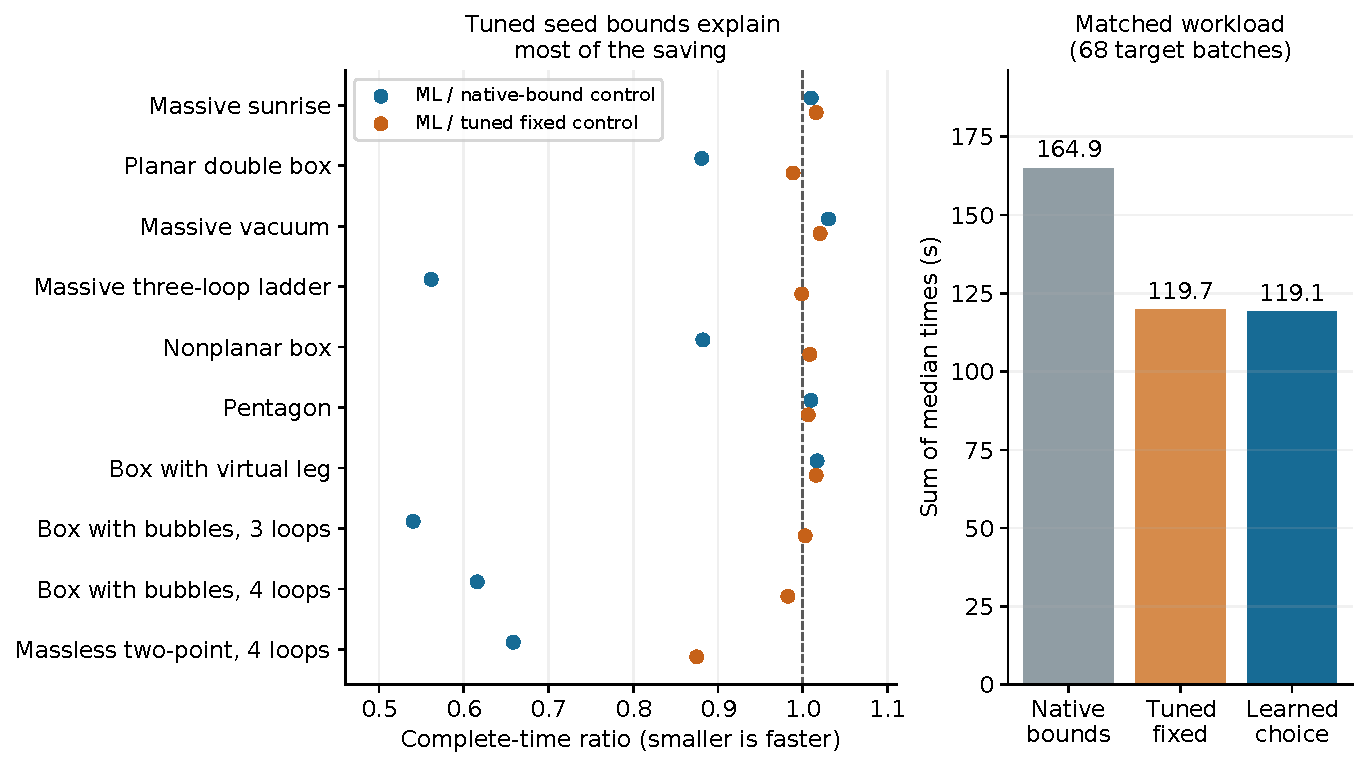
\includegraphics[width=\linewidth]{paper_figures/learned_bounds_times.pdf}
\caption{The left panel shows how the learned choice changes complete time for each graph; a ratio below one means a saving. The right panel shows the summed matched workload time. Both controls disable all learned choices. The graph labels refer to the explicit denominator definitions in the appendices.}
\label{fig:learned-bounds-times}
\end{figure}

The learned-to-control time ratios have descriptive 95\% intervals $[0.625, 0.885]$ against native bounds and $[0.980, 1.006]$ against the tuned fixed settings when whole graphs are resampled. Resampling repetitions within the fixed workload instead gives $[0.716, 0.727]$ and $[0.984, 1.006]$. The first calculation describes variation across this small graph collection; the second describes observed timing variation on these particular inputs. Neither interval proves a speedup on all integrals.

The summed generated-equation count changes from 2,029,994 under native bounds to 1,089,074 under learned choices, including equations from failed attempts. Average parameter loading and prediction take 7.067 and 0.836 milliseconds per learned request. Figure~\ref{fig:learned-bounds-effects} shows both the time ratios for each batch and the equation counts. The domain check and its time remain part of every learned request. The largest observed process-tree memory use is 946.8 MiB within the common limit.

\begin{figure}[!htbp]\centering
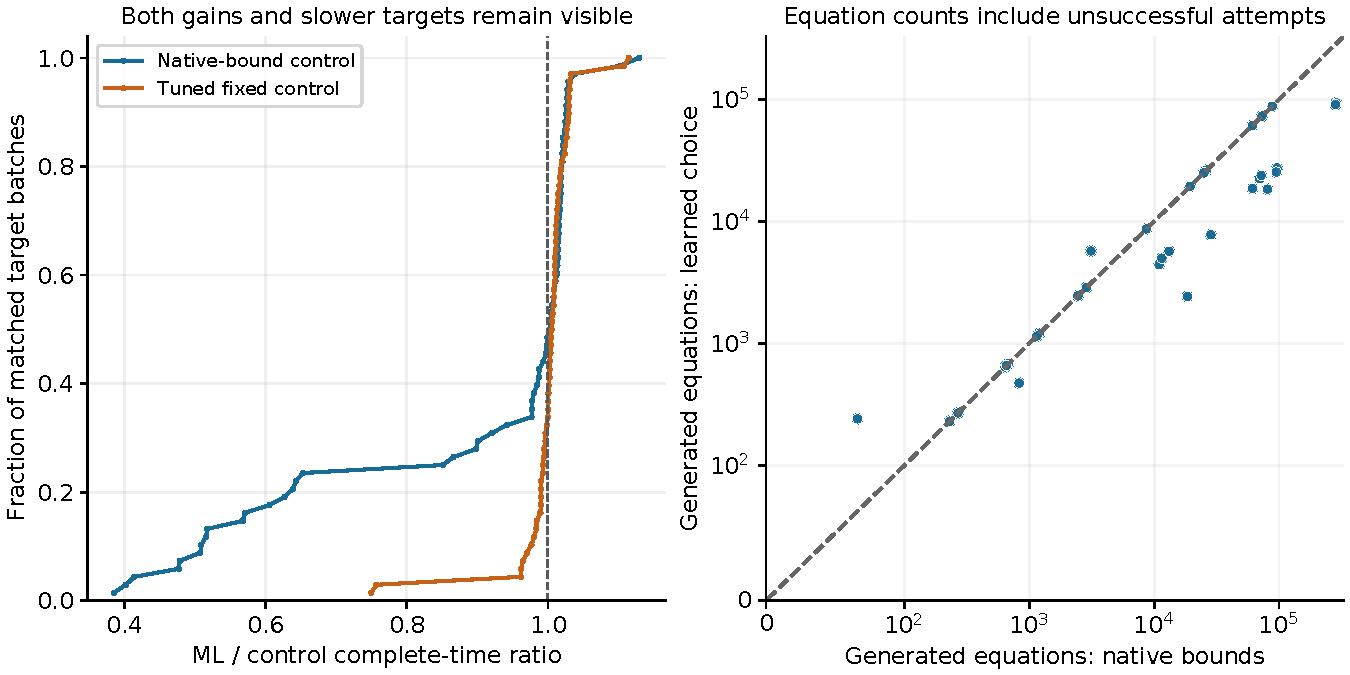
\includegraphics[width=\linewidth]{paper_figures/learned_bounds_effects.pdf}
\caption{Left: the distribution of batch time ratios retains every matched batch, including regressions. Right: generated equations under the learned and native-bound choices, with retries included. Points below the diagonal use fewer equations. The axes use a linear scale near zero and a logarithmic scale above 100 equations. Equation count explains part of the timing change but does not replace the complete-time measurement.}
\label{fig:learned-bounds-effects}
\end{figure}

Development, training-cost collection, validation, and their reference calculations take 1.37 hours of recorded calculation time, including 5.68 seconds for model fitting and selection. If future requests have the same mean saving as this matched workload, approximately 7295 requests would recover that cost relative to native bounds and 525989 relative to the fixed control. This extrapolation uses the measured workload and the derivation in Appendix~\ref{app:learned-bounds}; it is not a prediction for a different workload. The interval against the tuned fixed control includes equal time. Thus, this test establishes a saving from tuned seed settings but does not establish a reliable extra saving from learning which setting to use. The wider high-loop and symbolic coverage results retain the separate scope given in Section~\ref{sec:coverage}.

\subsection{Fresh application comparison}
A separate comparison starts a new application process for every request. It uses one fixed target pattern from each graph at the first reserved profile and three repetitions. The timer includes Python imports, input parsing, model loading, calculation, result storage, process exit, and coefficient checks. On 9 matched nontrivial batches, summed median time is 29.648 seconds for native bounds, 20.913 seconds for the previous published application, and 20.797 seconds for the new model. This is 29.9\% less time than the fresh native-bound application and 0.6\% less time than the previous application. The previous application retains its own validated portfolio and worker choices. Its comparison therefore measures the deployed workflow as a whole; the primary comparison above isolates the new learned choice.

\section{Learning which equations to construct after seed tuning}
\label{sec:equation-refinement}
The seed-bound experiment shows that tuning a fixed configuration explains most of its time saving. We therefore keep those tuned seed limits and train a model for a finer decision: whether to construct each equation inside the selected region. This comparison asks whether learned equation selection supplies an additional saving after the coarse seed region has already been improved.

\subsection{Model and integration with exact reduction}
Each candidate consists of a seed integral and one IBP or Lorentz-invariance operator. A classification tree uses the seventeen quantities in Table~\ref{tab:refinement-features}, including seed powers, target powers, distance to a target, and operator index. All these quantities are available before symbolic coefficient construction. The tree follows feature-threshold tests to a terminal node, called a leaf. The leaf score is the weighted positive fraction of its training examples, and Kira constructs the equation when that score meets the selected threshold. We also test a learned seed choice that retains every operator from a seed when at least one operator receives a score above the threshold. This uses the same trained scores and keeps more identities from each retained seed, which can prevent a failed reduction. Validation compares both uses of the model. Native symmetries, exact elimination, and back substitution remain in use. A failed attempt triggers the same tuned seed configuration with the filter disabled, followed by native and expanded bounds if needed. Thus the reported cost includes the consequences of an insufficient equation set.

The training label records whether the equation's integral support appears in Kira's final selected system. Support means the set of integrals with nonzero coefficients. This label is a proxy for usefulness and does not identify a unique necessary equation set. We collect new labels with the tuned seed settings because changing those settings changes which equations Kira can select. Collection uses a Kira build that records selected supports, and every collected reduction must agree with the independent exact reference. The timed comparisons use the same current build for both methods. The earlier filters frequently need a complete retry on these inputs, so their previous performance does not justify using them without new validation.

The four-loop box with bubbles has no completed label collection within the resource allowance, so it uses unfiltered reduction in this test. We preserve those collection failures. For the nine remaining structures, we fit eight shared classification trees and eight separate trees per graph~\cite{CART1984,Pedregosa2011Bounds}, with maximum depths 6, 10, 14, or 18 and minimum leaf populations 4 or 16, and a limit of 4,096 leaves. The data contain 137015 sampled equation records, including 39285 positive labels, from 66 training batches. Sampling weights preserve the native class proportions and give each batch equal total weight. The model receives no final reduction coefficients. Validation uses 33 separate batches, first to find filters that retain nearly all positive labels and then to measure complete reduction cost. A graph uses a learned seed or equation filter only when its median validation cost is at least 5\% below the same tuned calculation with all ML disabled. Appendix~\ref{app:equation-refinement} specifies the fitting, threshold selection, and recovery rules.

\subsection{Reserved comparison and the additional learned gain}
We freeze the trees, thresholds, graph choices, and domain limits before evaluating two new rational kinematic profiles, $h=525,526$. The dimension remains symbolic. The ten graph structures and target patterns are the same as in Appendix~\ref{app:learned-bounds}; the new profiles supply distinct kinematic requests. Some index patterns repeat training patterns, including the planar and nonplanar boxes at these two profiles. This is a test within known structures at one through four loops. A separate comparison below changes the target-index batches as well. As in the seed-bound study, each timed request receives a common master basis, and independent reference coefficients enter only the final exact comparison.

Both methods use the same executable, tuned seed limits, native row choices, exact implementation improvements, worker count, and recovery limits. The control disables every learned selector. Five repetitions alternate the order of the two methods. Time includes policy loading, the domain check, equation prediction and generation, exact algebra, verification, retries, and cleanup. Initial Python imports and construction of the common reference basis remain outside this repeated timer. A domain check disables filtering for an unrecognized ordered graph or target complexity outside the saved ranges.

The reserved grid has 74 requests. It supplies 68 matched nontrivial batches, with 4 failed reference checks, 0 incomplete timed batches, and 2 identity-only batches kept separately. All successful outputs pass exact coefficient comparisons: 700 completions among 700 timed requests, with 15430 comparisons. Table~\ref{tab:equation-refinement} retains each graph, including any slower result.

\begin{table}[!htbp]\centering\small
\caption{Additional effect of the equation model after fixed seed tuning. Times are sums of batch medians in seconds. ``Active'' counts batches on which the frozen policy enables filtering. A ratio below one means less complete time.}
\label{tab:equation-refinement}
\begin{tabular}{@{}lrrrrrr@{}}\toprule
Graph & Loops & Batches & Active & ML off & Policy & Ratio\\\midrule
Massive sunrise & 2 & 8 & 0 & 4.70 & 4.69 & 0.997\\
Planar double box & 2 & 8 & 8 & 18.78 & 15.79 & 0.841\\
Massive vacuum & 3 & 8 & 8 & 8.07 & 7.55 & 0.937\\
Massive three-loop ladder & 3 & 8 & 8 & 26.12 & 23.97 & 0.918\\
Nonplanar box & 2 & 8 & 8 & 38.74 & 37.07 & 0.957\\
Pentagon & 1 & 8 & 0 & 6.75 & 6.64 & 0.983\\
Box with virtual leg & 1 & 8 & 0 & 4.85 & 4.83 & 0.996\\
Box with bubbles, 3 loops & 3 & 6 & 0 & 9.48 & 9.50 & 1.002\\
Box with bubbles, 4 loops & 4 & 2 & 0 & 30.99 & 31.16 & 1.005\\
Massless two-point, 4 loops & 4 & 4 & 0 & 5.44 & 5.38 & 0.990\\
\bottomrule\end{tabular}
\end{table}

The full matched workload changes from 153.937 to 146.586 seconds, a time saving of 4.8\%. For the 32 batches on which the frozen policy enables a filter, the corresponding times are 91.707 and 84.384 seconds, giving 8.0\% less time. The 95\% intervals from resampling paired repetitions are $[0.946, 0.959]$ for the full workload ratio and $[0.916, 0.927]$ for the active subset. The active subset follows the pre-test policy and is not selected from the observed test speedups. These intervals describe timing variation on the tested requests, not generalization to arbitrary graphs.

\begin{figure}[!htbp]\centering
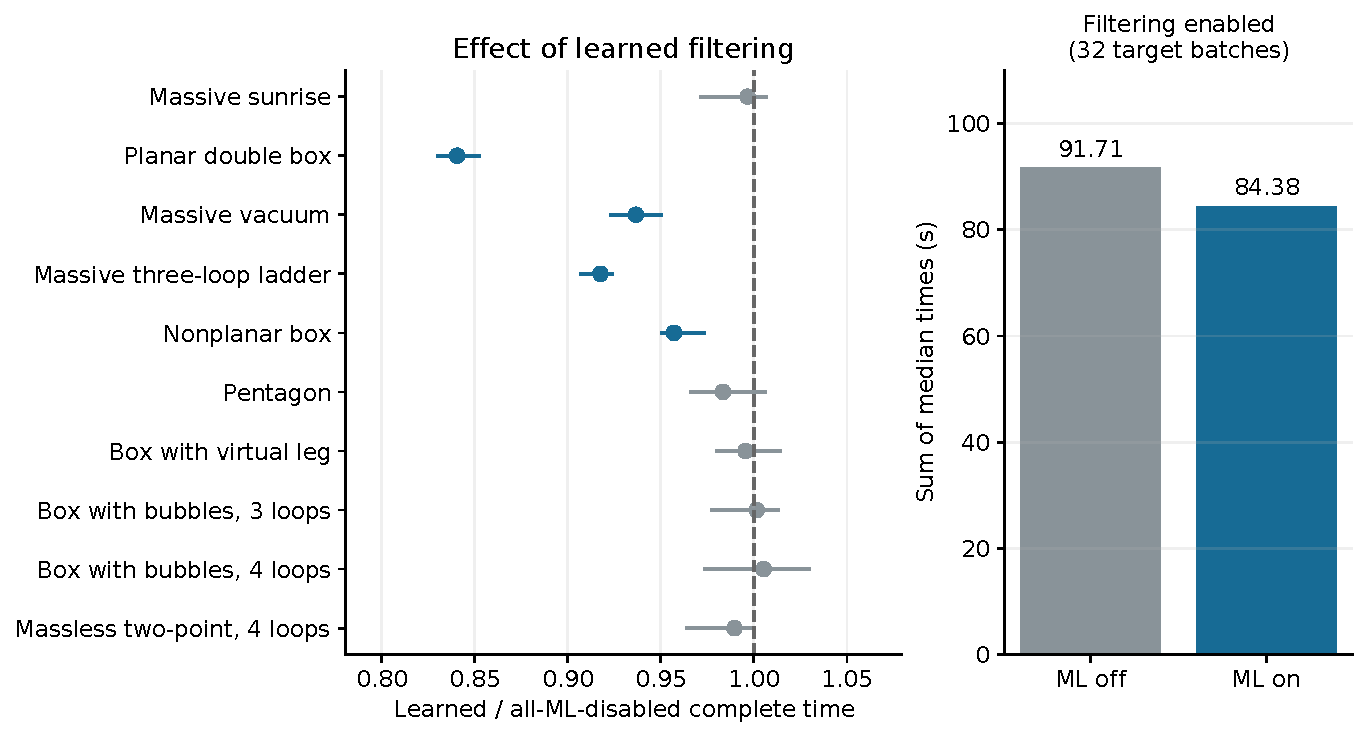
\includegraphics[width=\linewidth]{paper_figures/equation_refinement_times.pdf}
\caption{The left panel shows the complete-time ratio for every matched graph. Blue marks graphs with filtering enabled; grey marks graphs using the unchanged exact calculation. Horizontal intervals show the 95\% range from resampling paired repetitions within each graph. The right panel isolates the batches on which the preselected policy uses the trained filter. The control shares all exact optimizations and tuned seed settings, so the difference includes only the learned policy and its consequences.}
\label{fig:equation-refinement}
\end{figure}

On active requests, the filters reject 36.8\% of candidate construction calls, with a mean recorded filtering cost of 16.972 milliseconds per request. Repeated generation passes contribute to this count. Recovery can construct some rejected equations later, and its full cost remains in the timing comparison. The learned policy makes 5 recovery attempts in the reserved comparison. Recorded development, label collection, validation, and fitting take 39.2 minutes, excluding earlier seed-tuning costs. This expense precedes application and must be recovered over repeated use. A useful model on this collection does not establish a benefit for an unsupported topology, symbolic kinematics beyond the dimension, or all high-loop integrals. The separate wider coverage results retain their stated scope.

\subsection{Complete application launches}
A separate check starts a fresh application process for each request and supplies only the target definition and master basis. It uses the first supported reserved request for each graph where validation enabled filtering, with three rotated repetitions. These are a subset of the same reserved physical inputs. The timer includes Python startup, input parsing, model loading, output storage, process exit, and the exact coefficient check. Across 4 matched requests, summed median time changes from 21.835 seconds with all ML disabled to 18.946 seconds with the filter, giving a time saving of 13.2\%. This comparison checks the live application overhead; it does not add new graph structures to the physical scope.

\subsection{Transfer to new target-index batches}
The primary comparison changes kinematics but partly repeats the index patterns seen in training. To test index transfer separately, we keep the original fitted models, thresholds, and graph choices and define profiles $h=605,606$. We retain a batch only if its set of index vectors is absent from both training and validation and contains at least one individual index vector absent from those sets. We also remove repeated batches within each profile. These conditions select inputs from the graph structures enabled by the original validation; no primary test timing enters this selection. The selection rules and all resulting inputs are fixed before their reductions begin. The test therefore changes the indices within known graph structures and degree ranges, while transfer to new topologies remains untested.

Each request receives the same reference reduction and enlarged-region check as the primary comparison. Three repetitions rotate the two methods. The live application reads only a target definition and a master basis. Time includes basis reading, policy loading, prediction, exact reduction, recovery, and coefficient checks; it excludes initial Python imports and reference construction. Both methods retain the same seed settings and exact implementation.

\begin{table}[!htbp]\centering\small
\caption{The unchanged learned policy on new index batches. Times are sums of batch medians in seconds. The control disables every learned selector.}
\label{tab:index-transfer}
\begin{tabular}{@{}lrrrr@{}}\toprule
Graph & Batches & ML off & Policy & Ratio\\\midrule
Planar double box & 6 & 14.644 & 14.614 & 0.998\\
Massive three-loop ladder & 6 & 21.815 & 19.833 & 0.909\\
Nonplanar box & 6 & 29.771 & 27.317 & 0.918\\
Massive vacuum & 6 & 6.066 & 5.714 & 0.942\\
\bottomrule\end{tabular}
\end{table}

The structural rule defines 24 requests, of which 24 give matched nontrivial reductions. The record retains 0 failed reference checks, 0 incomplete comparisons, and 0 identity-only batches. All 144 successful outputs among 144 timed requests pass exact comparison, with 5106 coefficient checks. The summed median time changes from 72.295 to 67.478 seconds, giving 6.7\% less time. The 95\% paired-repetition interval for the learned-to-control ratio is $[0.928, 0.940]$. Table~\ref{tab:index-transfer} retains every matched graph, including any slower result. This check provides separate evidence about changes in target indices and is not combined with the primary timings to form a cumulative speedup.

\section{Learning which targets to reduce together}
\label{sec:batch-policy}
The equation filters reduce work inside a seed region, but the targets grouped in one request also determine that region. A batch can contain targets with high denominator powers and other targets with high numerator rank. Their combined limits can generate equations that neither group needs separately. Dividing the batch can avoid these equations, while repeating preparation and shared algebra can make an unnecessary division slower. We therefore train a model to choose the division from measured complete reduction time. Recent tube-seeding work also uses target groups to control reduction cost~\cite{TubeSeeding2026}; the present method uses ordinary Kira seed regions and the already checked equation filters.

\subsection{Model and integration with Kira}
The model compares five ways to divide a batch: keep all targets together, group equal numerator ranks, group equal extra denominator powers, group equal sectors, or use consecutive groups of at most three targets. A sixth candidate keeps the batch together and disables the equation filter, allowing the new model to avoid an expensive filter or retry. It receives 32 quantities that describe the physical family, the requested powers, and their distribution across the batch. It predicts the complete relative cost of each choice before Kira generates any equations. Each selected group then uses the same fixed seed policy and native row elimination as the preceding method. The existing equation filter acts only when enabled and when the group lies inside its original checked domain. We merge the resulting exact master coefficients after checking that every target has completed.

We compare regression trees, random forests, and extremely randomized forests~\cite{CART1984,Breiman2001Forest,Geurts2006ExtraTrees}. A tree compares the input quantities with learned thresholds and returns predicted costs from the final group of training examples. A forest averages the predictions of several trees. Here each prediction contains six log-cost ratios: the logarithm of a candidate's complete time divided by the time of the undivided batch. Training uses 49 batches, and separate validation uses 49 batches. The candidate with the smallest validation cost is an extremely randomized forest with 32 trees, at most 6 threshold levels, and at least one training example in each final group. Its chosen prediction margin is 0.02 in log-cost units, as defined in Appendix~\ref{app:batch-policy}, and its selected validation costs give 0.7\% less time than fixed partitions. No predictor reaches the required three-percent validation saving, so deployment uses the fixed partitions. The appendix specifies every partition, input, training objective, recovery rule, and physical request, and derives how the independently reduced groups give the complete target reduction.

The training labels include unsuccessful attempts and recovery. Reference construction supplies a common basis and checked coefficients before timing, but the solver receives only the basis and the target definitions. Reference coefficients enter the exact check after reduction. Recorded development, training, and validation reductions take 92.6 minutes, while fitting takes 8.86 seconds; these costs precede deployment and exclude reference construction. The median loading and decision cost in the timed test is 6.73 milliseconds.


Selecting the smallest recorded cost separately for every validation batch would lower the fixed-partition cost by 4.5\%. This comparison uses timing information available only after the calculations and describes the remaining opportunity within these six candidates. It does not describe a deployable predictor. Appendix~\ref{app:batch-policy} defines this retrospective bound.

\subsection{Controls and results}
The reserved comparison uses new rational profiles in the same ten structures at one through four loops, with symbolic dimension. The matched requests contain 1 to 11 targets each. Five repetitions rotate the methods through execution positions on the same worker. The previous method keeps each batch together. One fixed control chooses a partition per graph with the equation filters available; a second fixed control tunes its partitions independently with every ML model disabled. The comparison with the first fixed control measures the added batch-selection application, including its domain checks and loading cost. The second compares the combined workflow with tuned choices that perform no ML inference. All methods share the same exact implementation, basis, worker count, and checks.

Of 108 requests, 96 give matched nontrivial completions. There are 10 failed reference requests, 0 incomplete timed batches, and 2 matched identity-only batches. The comparison record contains 2450 successful results in 2450 calculations, with 90275 exact coefficient comparisons. Every successful result passes its reference check. A total of 34 requested index batches recur in this study's training or validation sets at different rational profiles. The test therefore measures new kinematics and a defined mixture of target batches within known graph structures.


The selected workflow actually calls an equation filter on 4 matched batches. On this subset it uses 7.0\% less time than the separately tuned ML-disabled control. This subset records filter use; its controls can also choose different fixed partitions. Its paired-repetition ratio interval is $[0.834, 1.018]$. This interval includes equal time and does not establish a reliable saving on this subset.


Two cluster allocations reached their time limits before completing all requests. We preserve the 76 complete comparison batches and resume the 22 remaining batches with unchanged models and timing rules. For an interrupted batch, we repeat every method and repetition on one worker. The 4 saved timings from its earlier partial comparison remain available separately and do not enter the ratios. Work assignment uses validation costs only.

Summed batch median time changes from 383.760 seconds for the previous undivided workflow to 389.368 seconds for the selected workflow, giving 1.5\% more time. The fixed control with filters takes 386.251 seconds, and the independently tuned all-ML-disabled control takes 389.826 seconds. Relative to these controls, the selected workflow uses 0.8\% more time and 0.1\% less time, respectively. The selected-to-fixed ratio has a paired-repetition interval of $[0.988, 1.035]$, and the ratio to the all-ML-disabled control has interval $[0.986, 1.025]$. Validation disables the new predictor, so this comparison establishes no additional ML gain from batch selection. Table~\ref{tab:batch-policy} shows the separate graph results, including regressions.


The recorded generation counts sum to 2,429,859 equations for the previous workflow, 2,514,300 for the tuned ML-disabled control, and 2,494,576 for the selected workflow. These are sums of per-batch median counters over reported generation passes, including repeated passes and retries. They describe generated equations rather than the total number of arithmetic operations. Complete time remains the criterion for retaining a model.

\begin{table}[!htbp]\centering\small
\caption{Sum of median complete times in seconds on matched batches. Previous keeps each batch together. Fixed uses one partition per graph with filters. ML off tunes partitions separately with every model disabled. Selected uses the frozen deployment choice.}
\label{tab:batch-policy}
\begin{tabular}{@{}lrrrrr@{}}\toprule
Graph & Batches & Previous & Fixed & ML off & Selected\\\midrule
Three-loop bubble box & 12 & 27.83 & 27.69 & 28.03 & 28.06\\
Four-loop bubble box & 2 & 18.69 & 19.61 & 18.99 & 19.75\\
Planar double box & 12 & 37.29 & 39.87 & 40.36 & 40.05\\
Massive ladder & 12 & 98.23 & 103.36 & 102.32 & 102.17\\
Massless two-point & 10 & 30.38 & 26.66 & 26.76 & 26.56\\
Nonplanar box & 12 & 138.39 & 135.97 & 139.94 & 139.29\\
Virtuality box & 8 & 5.31 & 5.62 & 5.64 & 5.70\\
Pentagon & 8 & 6.20 & 6.07 & 6.12 & 5.99\\
Sunrise & 12 & 13.12 & 12.97 & 12.91 & 13.55\\
Massive vacuum & 8 & 8.31 & 8.41 & 8.76 & 8.23\\
\bottomrule\end{tabular}
\end{table}
\begin{figure}[!htbp]\centering
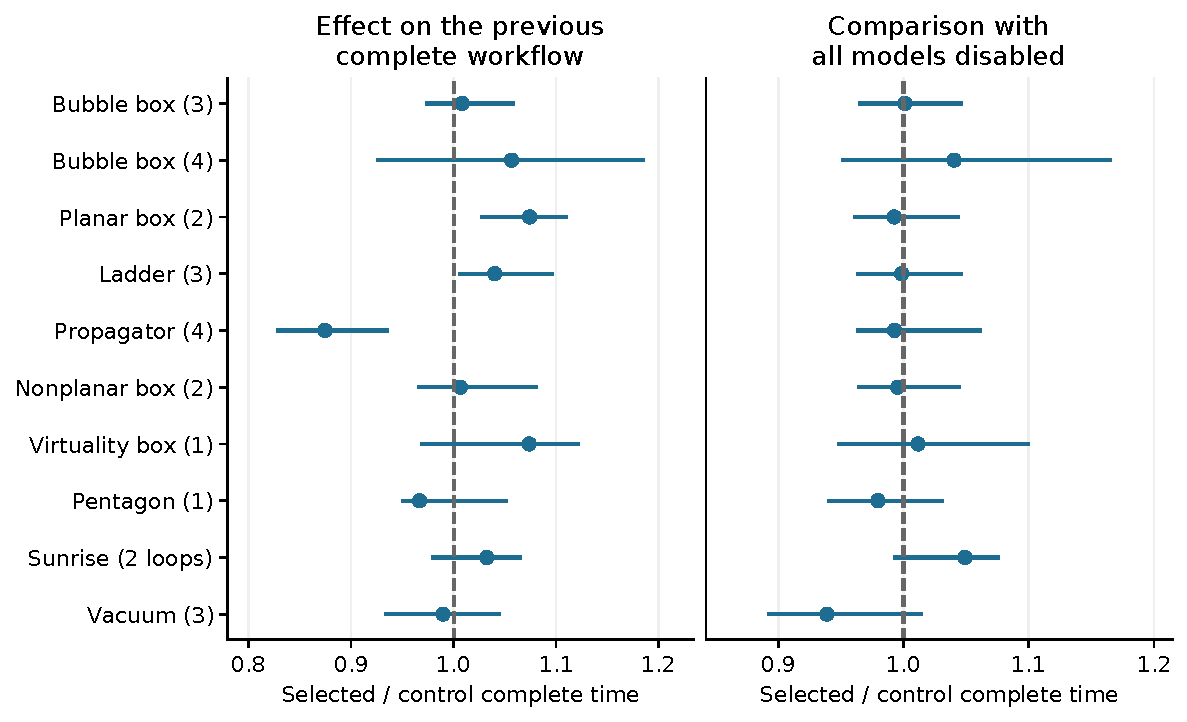
\includegraphics[width=\linewidth]{paper_figures/batch_policy_times.pdf}
\caption{The left panel compares the selected complete workflow with the previous undivided workflow. The right panel compares it with independently tuned fixed partitions with every model disabled. Values below one indicate less time; the dashed line marks equal time. Segments describe paired repetition variation on this workload. Validation disables the new batch predictor; the selected workflow uses the retained fixed partitions and equation-filter settings.}
\label{fig:batch-policy}
\end{figure}
\FloatBarrier

A separate application check starts a new Python process for each request and includes imports, model loading, input and output, and exact checks. Deployment loads only the parts of the frozen policy that it uses: when validation disables the predictor, it retains the fixed choices and domain limits and omits the unused tree arrays. We check that this compact form gives the same choices on every training, validation, and reserved input, without reading reserved timing outcomes. The repeated comparison above retains the original frozen application; this separate check uses the compact form. It completes 36 timed requests over 4 matched batches and gives 1.2\% less time than the previous workflow. These batches are a predeclared subset of the reserved inputs, so this check measures application overhead without adding evidence for new topologies.

The new study extends the batch sizes tested by the earlier equation-filter comparison. It still supplies a master basis and keeps the kinematic invariants rational. General symbolic scattering, arbitrary higher-loop structures, and globally optimal partitions remain outside this evidence. The earlier restricted vacuum recurrence covers its stated one-through-twelve-loop family separately, and its speedup cannot be multiplied by the ratios measured here.

\section{Learning sparse seed regions from reduction time}
\label{sec:seed-geometry}
The batch study leaves little additional saving among its predefined partitions. We therefore change the equations available to Kira more directly. A learned boundary selects individual seeds around the requested numerator powers before equation generation. Kira then applies its usual IBP operators to those seeds. This follows the motivation of sparse target-dependent seeding~\cite{TubeSeeding2026}, while the boundary parameters in this study are fitted through complete reductions with symbolic dimension.

\subsection{The seed model and its training data}
The model describes a surrounding region around each target's numerator-power box. Its width can depend on the seed rank and on how many physical propagators are absent from its sector. It also controls the largest seed rank in each sector. Appendix~\ref{app:seed-geometry} defines these boundaries, derives the distance used by the model, and gives a counting example that explains why a narrow region can avoid many seeds at higher numerator rank.

We first fit the boundary parameters through evolutionary search. Each proposal runs Kira and receives a score from the measured time needed to reach the prescribed masters and pass an exact coefficient check. The score includes unsuccessful attempts and native recovery. Thus the labels describe completed calculations rather than membership in a previously selected equation set. Three training requests per graph start this search; separate validation selects the first fitted boundary. An independent planar-box comparison then tests that boundary on eight new kinematic requests.

The second stage adds twelve training requests per graph and fits models that predict the cost of different seed boundaries. These requests contain single-direction and distributed numerators of ranks two, three, and four. The candidate boundaries include those found by the first search, independent changes to the rank allowance, fixed surrounding widths, and unfiltered Kira. Trees and forests predict the log complete-time ratio of each candidate~\cite{CART1984,Breiman2001Forest,Geurts2006ExtraTrees}. Ten validation requests per graph select the model, its decision margin, and a fixed sparse control. The predictor is enabled only when validation gives at least three percent less recorded cost than that fixed control. When validation disables prediction, the deployed policy uses the selected fixed boundary. Table~\ref{tab:seed-geometry-models} gives the selected models. The independent timing tests include the cost of loading and applying them.

\begin{table}[!htbp]\centering\small
\caption{Cost predictors selected before the reserved comparisons. Each graph also has a separately selected fixed sparse control.}
\label{tab:seed-geometry-models}
\begin{tabular}{@{}llll@{}}\toprule
Graph & Predictor (depth) & Training requests & Deployment\\\midrule
Planar box & Tree (2) & 12 & Fixed boundary retained\\
Nonplanar box & Extra trees (2) & 12 & Enabled\\
\bottomrule\end{tabular}\end{table}

Validation enables request-dependent cost prediction for the nonplanar box. Other graph choices use their fixed sparse boundary.

\subsection{Independent reductions and controls}
The first evolved planar-box boundary gives 22.3\% less time, with a paired-repetition ratio interval of $[0.751, 0.813]$ relative to tuned native Kira. Relative to the fixed surrounding-width control, it gives 6.5\% less time, with a paired-repetition ratio interval of $[0.899, 0.980]$. This comparison contains 168 timed reductions, and all successful outputs pass exact checks. The boundary remains fixed throughout this test.

\begin{table}[!htbp]\centering\small
\caption{First independent planar-box comparison. Times are sums of per-request medians over eight requests, with seven repetitions per method. The learned boundary is fitted before this comparison.}
\label{tab:seed-geometry-initial}
\begin{tabular}{@{}lr@{}}\toprule
Method & Complete time (s)\\\midrule
Tuned native Kira & 37.893\\
Fixed surrounding width & 31.465\\
Evolved seed boundary & 29.424\\
\bottomrule\end{tabular}\end{table}

The second comparison uses 20 matched requests from the planar and nonplanar two-loop boxes, with seven repetitions per method. All methods use the same Kira executable, exact preparation, master basis, and native row elimination. The native control disables every learned choice. The fixed sparse control uses one validation-selected boundary per graph, including boundaries discovered during training, and performs no request-dependent cost prediction. The previous application retains the earlier published batch and equation policies. These controls separate the effect of sparse seeding from the added benefit of predicting which boundary to use for a particular target.

The complete selected workflow gives 22.2\% less time, with a paired-repetition ratio interval of $[0.764, 0.792]$ relative to tuned native Kira and 22.6\% less time, with a paired-repetition ratio interval of $[0.762, 0.789]$ relative to the previous application. Relative to the fixed sparse control, it gives 3.6\% less time, with a paired-repetition ratio interval of $[0.946, 0.981]$. Table~\ref{tab:seed-geometry-times} reports the measured times for both graphs. The comparison contains 560 timed reductions and 5600 exact coefficient comparisons. Failed reference requests number 0, and failed timed reductions number 0; these remain in the evidence record.

\begin{table}[!htbp]\centering\small
\caption{Sum of per-request median complete times, in seconds. Native uses the tuned outer bounds with all ML disabled. Fixed uses one sparse boundary per graph. Selected uses the frozen deployment policy.}
\label{tab:seed-geometry-times}
\begin{tabular}{@{}lrrrrr@{}}\toprule
Graph & Requests & Native & Previous & Fixed & Selected\\\midrule
Planar box & 10 & 20.986 & 21.072 & 15.742 & 15.802\\
Nonplanar box & 10 & 54.857 & 55.100 & 45.462 & 43.169\\
All matched & 20 & 75.843 & 76.172 & 61.203 & 58.972\\
\bottomrule\end{tabular}\end{table}

\begin{figure}[!htbp]\centering
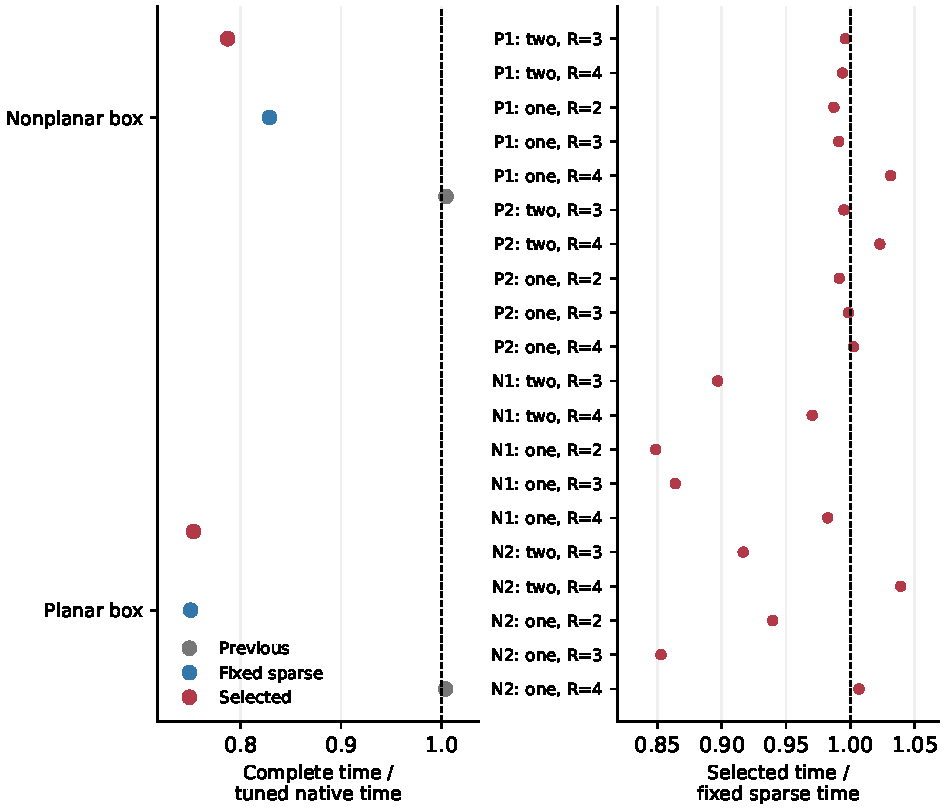
\includegraphics[width=\linewidth]{paper_figures/seed_geometry_times.pdf}
\caption{Left: complete-time ratios to tuned native Kira, summed within each graph. Right: the selected-to-fixed-sparse ratio for each reserved request. Labels P and N identify the planar and nonplanar graphs; 1 and 2 identify the two reserved kinematic profiles. Each label gives the number of powered numerator directions and the rank $R$. The dashed lines mark equal time. Values below one indicate a saving. The right panel shows the measured difference from using the fixed sparse rule.}
\label{fig:seed-geometry-times}
\end{figure}
\FloatBarrier

A separate application check starts a fresh process for each request and supplies only the physical definition, target indices, and master basis. It includes imports, model loading, input and output, process exit, and a subsequent exact check. It completes 48 runs over 4 matched requests. Its selected total is 15.774 seconds, compared with 27.897 seconds for native choices and 16.187 seconds for the fixed sparse control. These requests are a predefined subset of the reserved test, so they check application overhead without adding graph coverage.

The complete integrated application also passes 24 fresh-process checks. These use two of the reserved two-loop requests, one previously tested four-loop native request, and an eight-loop massless banana request. For the two-loop requests, the summed median complete time is 8.091 seconds, compared with 17.088 seconds for the preceding complete application. The other inputs check that the existing native and analytic methods remain available and exact. They do not extend the sparse model's fitted domain.

These results concern numerator ranks two through four, unit positive physical powers, rational kinematic values, symbolic dimension, and supplied bases in two known two-loop structures. The reported production times exclude offline training and construction of the independent reference basis. Some index patterns recur between training and testing. Development probes at other loop orders do not extend the fitted model's validated domain. The application retains its earlier exact methods and native fallback outside this domain. The comparison establishes the measured effects of the new seed policy; it does not establish a universal speedup or a globally optimal reduction path.

\section{Joint seed choices and exact scale reuse}
\label{sec:joint-policy}
The preceding study reduces unnecessary equation generation, but some sparse choices still require a repeated calculation. To reduce this cost, we train new policies that select a seed boundary and Kira configuration together, then compare them with the preceding ML application. Validation retains the preceding application for both graphs because neither replacement clears the required improvement threshold. We add an exact scaling relation that reuses a completed reduction at a different overall momentum scale. The retained ML application performs the first reduction, and the exact identity can remove later reductions with matching dimensionless kinematics.

\subsection{Learning a complete reduction configuration}
The candidate configurations combine sparse boundaries with Kira's integral-ordering and internal propagator-permutation options~\cite{Kira2,Kira3}. The model chooses a configuration before equation generation. Kira then uses its native elimination procedure, and the earlier learned row policy remains omitted. Development reductions determine the candidate set, while separate training reductions supply the complete time of each candidate, including failed attempts and recovery. This follows the same cost-based principle as the preceding seed-boundary study; sparse seed searches also motivate the work in Ref.~\cite{TubeSeeding2026}.

We compare regression trees, random forests, and extremely randomized trees~\cite{CART1984,Breiman2001Forest,Geurts2006ExtraTrees}. Each predicts candidate log-time ratios from 68 features describing the integral family and target powers. Validation selects the model, its decision margin, and a fixed configuration for each graph. The model is enabled only when validation gives at least 2\% less time than the fixed choice, and the new deployment must also improve on the preceding application by at least 2\%. Otherwise the preceding application remains in use. The planar replacement gives 0.9\% less time than the preceding application on validation. The nonplanar replacement gives 0.9\% less time than the preceding application on validation. Both improvements fall below the predefined threshold, so the following tests retain the preceding ML decisions. Appendix~\ref{app:joint-policy} specifies the candidates, inputs, training objective, and exact target definitions.

\begin{table}[!htbp]\centering\small
\caption{Models selected before testing. The deployment condition uses validation times only.}
\label{tab:joint-models}
\begin{tabular}{@{}p{0.13\linewidth}p{0.41\linewidth}p{0.38\linewidth}@{}}\toprule
Graph & Selected fitted model & Deployment\\\midrule
Planar & Regression tree, maximum depth 2 & Previous application retained\\
Nonplanar & 48 extremely randomized trees, maximum depth 4 & Previous application retained\\
\bottomrule\end{tabular}\end{table}

\subsection{First-request time on separate test inputs}
The test contains 24 requests from the same two massless two-loop graph structures, at new rational kinematic profiles. Targets have unit positive physical powers and numerator ranks two through four, with either one or two powered auxiliary entries. Each graph has twelve training, twelve validation, and twelve test requests. Some target index patterns recur between the splits. Five repetitions rotate the four methods on the same worker for each request, using one Kira thread. The main test performs no result reuse.

The native control disables all ML and uses the tuned outer seed bounds. The fixed control uses one validation-selected seed and ordering configuration per graph, with no prediction or model loading. The previous control uses the preceding complete application. The selected method wraps that same application with the new input checks and optional reuse interface. Since validation disabled both replacements, its first-request comparison with the previous control measures this added interface and timing variation. All methods receive the same master basis, and the timer includes input preparation, configuration selection, equation generation, exact algebra, coefficient checks, and every retry. Master discovery and offline model training precede these production timings.

Table~\ref{tab:joint-times} gives the sum of per-request medians. Relative to the preceding application, the selected method gives 1.2\% less time, with time-ratio interval $[0.975,1.024]$. Relative to tuned native Kira, it gives 18.0\% less time, with time-ratio interval $[0.806,0.841]$. Its comparison with the fixed control gives 5.7\% less time, with time-ratio interval $[0.926,0.966]$. These intervals use paired resampling of the five repetitions on the fixed test workload. They describe timing variation and do not establish performance for unseen graph structures. All 480 timed reductions pass 4800 exact coefficient comparisons. The retained data include individual slower requests and all failed first attempts.

Across the five repetitions, the preceding application makes 5 additional reduction attempts, the fixed control makes 45, and the selected method makes 5. These counts identify repeated algebra caused by an insufficient first choice; their costs are already included in the reported times.

The selected-to-fixed differences include configuration choices inherited from the preceding application. These comparisons therefore assess complete configurations and provide no evidence of a gain from the new predictors.

\begin{table}[!htbp]\centering\small
\caption{Complete first-request times, in seconds, summed over per-request medians. There are twelve reserved requests per graph.}
\label{tab:joint-times}
\begin{tabular}{@{}lrrrr@{}}\toprule
Graph & Tuned native & Previous & Fixed & Selected\\\midrule
Planar & 33.082 & 25.449 & 25.326 & 25.406\\
Nonplanar & 78.584 & 67.219 & 71.816 & 66.161\\
Total & 111.666 & 92.668 & 97.142 & 91.567\\
\bottomrule\end{tabular}\end{table}

\begin{figure}[!htbp]\centering
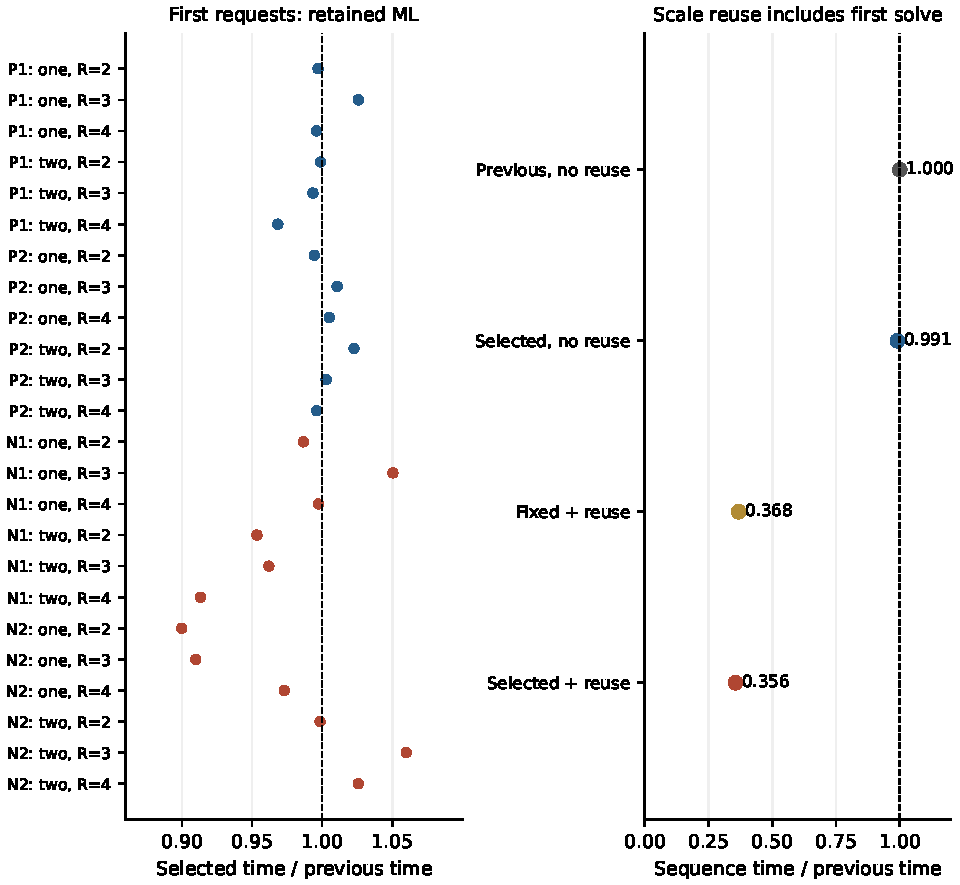
\includegraphics[width=\linewidth]{paper_figures/joint_policy_times.pdf}
\caption{Left: the selected-to-previous complete-time ratio for each reserved request, including slower cases. P and N identify the planar and nonplanar graphs, 1 and 2 identify the two kinematic profiles, and the labels give the numerator pattern and rank. Right: aggregate time for the four scale sequences, normalized to the preceding application without reuse. Every sequence includes its first Kira reduction. Dashed lines mark equal time. The panels have separate workloads and their ratios cannot be multiplied.}
\label{fig:joint-times}
\end{figure}
\FloatBarrier

\subsection{Exact reuse when only the overall scale changes}
For a massless family with homogeneous quadratic inverse propagators, a common positive change of all external scalar products gives an exact relation between reduction coefficients. If $\boldsymbol b_m$ is the index vector of master $m$, define $\nu(\boldsymbol a)=\sum_i a_i$. Then
\begin{equation}
 r_{\boldsymbol a m}(\lambda\boldsymbol x,d)
 =\lambda^{\nu(\boldsymbol b_m)-\nu(\boldsymbol a)}
  r_{\boldsymbol a m}(\boldsymbol x,d),\qquad\lambda>0.
 \label{eq:joint-scale-rule}
\end{equation}
Appendix~\ref{app:joint-policy} derives this identity by scaling the integration momenta. Its exponent is an integer, and a rational scale therefore gives an exact rational multiplier. The application checks the graph, target indices, supplied basis, and every dimensionless kinematic ratio before reusing an earlier result. Changed ratios, masses, or symbolic kinematic values continue through the reduction application. Reuse supplies no benefit before a matching exact result exists.

We test four predefined rank-four requests, two from each graph, in sequences with scale factors $1$, $3/2$, and $2$. Each sequence starts a fresh process and includes the initial Kira reduction, imports, model loading, input and output, exact transformation, and the subsequent independent coefficient checks. Three repetitions and four methods give 48 measured sequences containing 144 requests. Independent native reductions at every scale supply the checks; their coefficients never enter the application inputs.

We sum the median sequence times over the four base requests. Under this measure, the selected policy with scale reuse uses 28.496 seconds, compared with 80.073 seconds for the preceding application without reuse and 79.334 seconds for the selected policy without reuse. The resulting change relative to the preceding application is 64.4\% less time, with time-ratio interval $[0.334,0.390]$, while reuse alone changes the selected policy's time by 64.1\% less time, with time-ratio interval $[0.350,0.383]$. A fixed configuration with the same exact reuse uses 29.466 seconds; the selected-to-fixed-reuse comparison gives 3.3\% less time, with time-ratio interval $[0.770,1.049]$. All transformed outputs pass exact checks. These sequence results measure the benefit of repeated dimensionless kinematics, and remain separate from the first-request model comparison.

The deployed application combines the retained ML application with this exact reuse and retains the existing analytic and native paths outside its fitted domain. Eight further fresh-process checks reproduce the earlier four-loop native and eight-loop analytic results. These checks preserve existing behavior and do not extend the new model's fitted range. The new timing evidence covers known two-loop boxes, rational kinematics, symbolic dimension, and supplied bases. It does not establish a fastest possible strategy for arbitrary integrals or unrestricted loop order.

\section{Broader tests of the frozen application}
\label{sec:extended-coverage}
The earlier gains concern selected graph structures and target patterns. We now keep the deployed models and all decision rules fixed and test a wider set of physical inputs. The expanded test defines 84 native family requests at one through twelve loops. 29 requests complete all methods and exact checks, while 36 exceed the current 31-index interface limit. The remaining requests retain their recorded failures. The separate analytic test verifies 24 scalar massless two-point batches, covering every loop order from one through twelve at both rational and symbolic momentum. A loop label alone therefore does not specify the demonstrated scope: the graph, masses, external momenta, target powers, and method also matter.

\subsection{Physical inputs and checks}
The native grid contains one-mass and fully massive vacuum families, massless and massive two-point families, four-point ladders, and boxes with bubble subgraphs. It also contains nonplanar boxes, pentagons, and boxes with one external virtuality. Rational profiles differ from those in the preceding studies. Selected low-loop cases keep the independent masses and momentum invariants symbolic. Appendix~\ref{app:extended-coverage} gives the target sets and parameter choices, using the previously defined denominators.

Each eligible request first runs Kira with expanded seeds and no preferred master basis. A second reduction changes the integral ordering and increases the numerator bound, then checks every coefficient in the discovered basis. This agreement tests stability within those two seed regions; it does not prove that every surviving master is independent under all possible IBP identities. The reference stage records 13 time-limit failures and 6 Kira allocation failures. The latter occur during topology preparation under the address-space cap, before a learned reduction decision is tested. These failures therefore identify preparation and resource limits, rather than model prediction errors. The three timed methods then receive that common basis. Kira generates their equations and performs the exact reduction, as in its standard reduction procedure~\cite{KiraOriginal,Kira3}.

The native control disables learned choices and uses the current exact implementation with fixed bounds. The previous and selected applications use their unchanged published policies. Each run starts a fresh process, and its time includes imports, input preparation, model loading, equation generation, algebra, coefficient checks, retries, and process exit. Every method loads the common application modules, including the native and direct-formula controls. These are complete times for the same interface, rather than timings of the Kira executable alone. The comparison includes costs that can matter for small requests. Master discovery and the independent reference calculation remain separate. Three repetitions rotate method order on the same worker for each case. Each native attempt has a 30-second budget, a 32 MiB temporary-storage limit, and the existing memory guard. The runner reserves ten seconds for completion and cleanup, leaving at most twenty seconds for the Kira process. A failure stops further repetitions of that method, and remains in the coverage count.

\begin{table}[!htbp]\centering\small
\caption{Outcomes for the complete predefined native grid. Rejected inputs have no timed Kira reduction.}
\label{tab:extended-coverage}
\begin{tabular}{@{}lr@{}}\toprule
Outcome & Requests\\\midrule
All methods verified & 29\\
Reference limit or failure & 14\\
Reference check failure & 5\\
Input index limit & 36\\
\bottomrule\end{tabular}\end{table}

\begin{table}[!htbp]\centering\small
\caption{Results by loop order. Native verified counts require all methods and reference checks. A dash means no matched nontrivial native timing comparison. Analytic checks cover the stated scalar massless two-point family.}
\label{tab:extended-loops}
\begin{tabular}{@{}rrrrr@{}}\toprule
Loops & Native verified/requested & Matched & Time ratio & Analytic passed\\\midrule
1 & 12/12 & 12 & 0.988 & 2/2\\
2 & 10/12 & 10 & 1.020 & 2/2\\
3 & 4/6 & 4 & 0.918 & 2/2\\
4 & 3/6 & 3 & 1.038 & 2/2\\
5 & 0/6 & 0 & -- & 2/2\\
6 & 0/6 & 0 & -- & 2/2\\
7 & 0/6 & 0 & -- & 2/2\\
8 & 0/6 & 0 & -- & 2/2\\
9 & 0/6 & 0 & -- & 2/2\\
10 & 0/6 & 0 & -- & 2/2\\
11 & 0/6 & 0 & -- & 2/2\\
12 & 0/6 & 0 & -- & 2/2\\
\bottomrule\end{tabular}\end{table}

\subsection{Complete application times}
The matched nontrivial set contains 29 requests for which all three repetitions of all methods pass the exact coefficient checks. A nontrivial reduction has at least one nonzero target expression beyond the unchanged target itself. We report the sum of per-request median times, using the definition in Appendix~\ref{app:coverage}. Identity-only answers and failed requests do not enter this time ratio. The two single-target rank-three box requests lack fully checked references under the common limits and therefore supply no new timing comparison for the learned sparse-seed route.

\begin{table}[!htbp]\centering\small
\caption{Complete times on the matched nontrivial requests. Ratios compare selected time with native time; a value below one means less time.}
\label{tab:extended-times}
\begin{tabular}{@{}lrrrr@{}}\toprule
Family & Requests & Native (s) & Selected (s) & Ratio\\\midrule
bubble box & 1 & 1.077 & 1.295 & 1.202\\
ladder & 4 & 6.786 & 6.755 & 0.995\\
nonplanar box & 2 & 11.028 & 11.246 & 1.020\\
one mass box & 2 & 2.228 & 2.386 & 1.071\\
pentagon & 2 & 2.915 & 2.582 & 0.886\\
propagator massive & 6 & 9.798 & 9.985 & 1.019\\
propagator massless & 4 & 4.436 & 4.155 & 0.937\\
vacuum all mass & 3 & 5.081 & 5.076 & 0.999\\
vacuum one mass & 5 & 5.548 & 5.550 & 1.000\\
\midrule
All matched & 29 & 48.896 & 49.030 & 1.003\\
\bottomrule\end{tabular}\end{table}

The previous application takes 48.136 seconds on the same set. The selected application's total differs from the native total by 0.3\%, and the timing interval includes equal time. The selected-to-native time ratio is 1.003, with a paired-repetition resampling interval [0.968, 1.073]. The interval describes timing variation for these fixed cases; it does not estimate coverage of all integral families. Reference discovery takes a further 71.653 seconds, and its independent check takes 117.521 seconds. Adding the same measured discovery work to each method gives 120.549 seconds for the native control and 120.684 seconds for the selected application. This last comparison includes discovery once per request and does not represent a learned master-discovery method.

These are comparisons of complete deployed configurations. Outside the fitted domain, the selected application can take an exact analytic route or fall back to native choices. In the matched set, 2 cases use the analytic formula and the remaining cases use native choices. No matched case activates a learned seed, batch, or equation decision. The frozen domain checks and validation gates determine these routes. This comparison therefore checks application coverage and fallback behavior, and its time difference supplies no evidence of a learned gain on these new targets. The earlier matched filter and sparse-seed controls remain the evidence for isolated learned gains.

\begin{figure}[!htbp]\centering
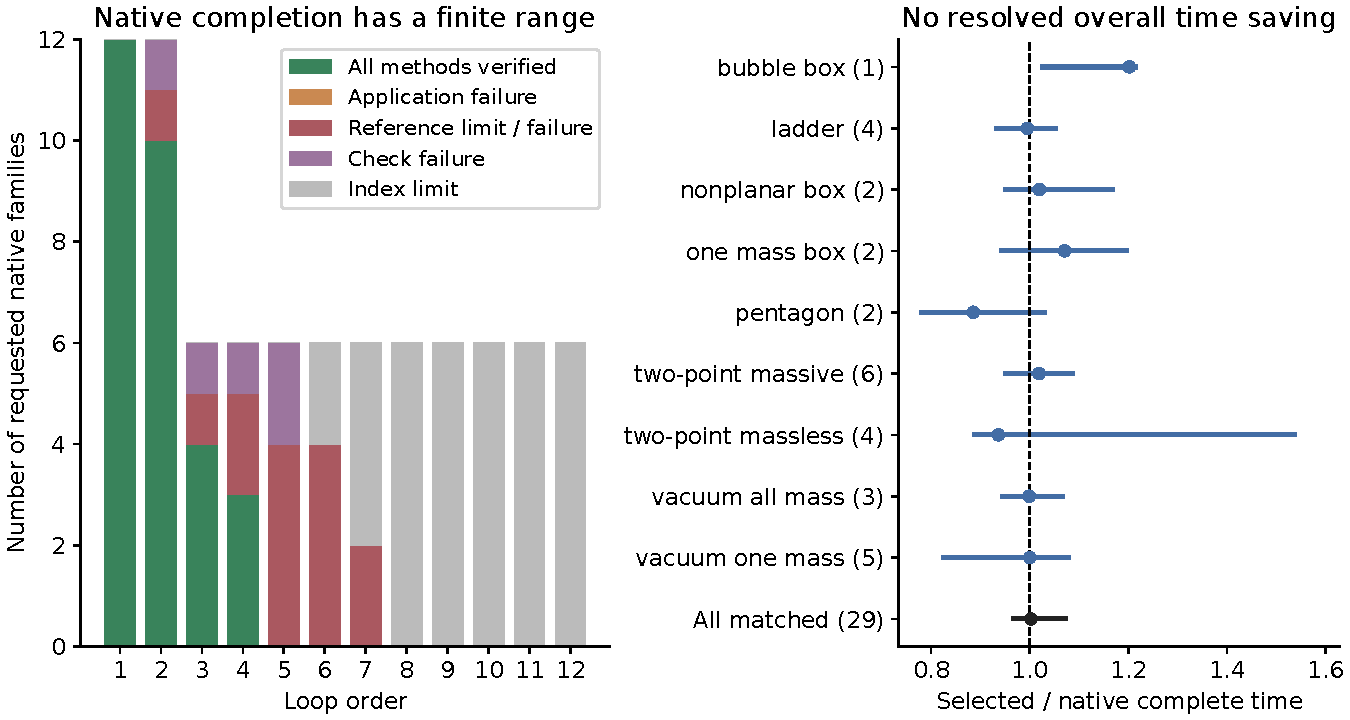
\includegraphics[width=\linewidth]{paper_figures/extended_coverage.pdf}
\caption{Left: every requested native family remains in the coverage count, including failures and input limits. Right: time-ratio points and paired-repetition intervals use only matched nontrivial cases, with case counts in parentheses. The dashed line marks equal time. The panels distinguish whether a calculation finishes from how long a completed calculation takes.}
\label{fig:extended-coverage}
\end{figure}\FloatBarrier

\subsection{Exact checks at every studied loop order}
The analytic test uses the scalar massless two-point family of Appendix~\ref{app:banana} and four target patterns at each loop order, with either a new rational value of $p^2$ or symbolic $p^2$. An independently implemented recurrence raises one propagator power at a time and checks each exact coefficient returned by the frozen application. Appendix~\ref{app:extended-coverage} derives this recurrence. All 24 batches pass, with four targets per batch and three repetitions of the direct formula, previous application, and selected application.

These inputs contain only the physical denominators. The analytic formula needs no auxiliary numerator coordinates, while general native IBP generation uses a complete scalar-product basis. For that complete representation, the current interface reaches its index limit at lower loop order. The twelve-loop analytic checks therefore verify the stated scalar family and exact route; they do not establish general native twelve-loop reductions or learned speedups at twelve loops.

\subsection{Reuse on the additional physical inputs}
Four base requests are fixed before testing: planar and nonplanar two-loop rank-three boxes, a one-loop ladder, and a two-loop massless two-point family. Each sequence changes all external scalar products by factors $1$, $3/2$, and $2$. Independent native references check each scale. The application can reuse only graph signatures already supported by the frozen scaling rule. Every measured sequence includes its first reduction and three repetitions rotate method order.

2 of the four sequences complete every paired method. Their summed median times are 4.601 seconds for the previous application, 4.581 seconds for the selected application without reuse, and 4.546 seconds with reuse. The ratio of selected reuse time to previous time is 0.988. The completed sequences record 0 reused outputs across the three repetitions. The retained records include any sequence that fails to obtain a checked reference. The completed sequences have no reuse hits because their graphs lie outside the current scale-cache domain. The two rank-three box sequences lack checked references within the limits, so this extension provides no new measurement of the reuse benefit. It checks sequence processing and the domain rules without new model training or a changed policy.

The full extension retains 495 successful measured calls and 0 failed measured calls, excluding the independent native references. The exact checks compare 6399 coefficient pairs. The result states where the existing method works under the specified limits. General reductions for every topology and arbitrary loop order remain unverified.

\section{Learning seed costs for a wider set of targets}
\label{sec:family-cost}
The broad test in Section~\ref{sec:extended-coverage} showed that the earlier models often fell back to native choices. We therefore extend cost training to vacuum, two-point, and scattering families, and make the decision before Kira generates equations. The new comparison asks whether a learned choice can improve on a separately tuned fixed choice for each family. Kira's existing seeding and equation selection remain the starting point~\cite{Kira3}, and every selected calculation retains exact algebra and recovery.

\subsection{Training and integration}
Each target batch has either two extra denominator powers or one extra denominator power with one numerator power when an auxiliary coordinate exists. We shift these powers across up to three lines. The training grid contains 22 labelled family-and-loop entries at one through four loops. The family definitions follow Appendices~\ref{app:coverage} and~\ref{app:families}; Appendix~\ref{app:family-cost} specifies the new profiles and target construction. These entries have rational external invariants and symbolic dimension. The two-loop ladder and planar double-box entries share a denominator routing and use different assignments of the external invariants. Thus the entry count does not count distinct graph topologies.

The model predicts the measured cost of ten seed settings, using loop order, denominator structure, target count, powers, and numerator positions. We fit shared decision trees and family-specific one-split cost trees, as well as random forests~\cite{Breiman2001Forest}, and extremely randomized trees~\cite{Geurts2006ExtraTrees}. The training set contains 111 complete cost examples from earlier training records and a new parameter profile. Separate validation selects the tree model, decision margin, and fixed control for each family. We retain a candidate model when it reduces the summed validation time for the two target shapes by at least 3\% relative to that family's best fixed setting. We then confirm each proposed learned gain on profile $h=1113$, using three repetitions. We retain the learned choice only if it again saves at least 3\% in total and neither target shape is more than 3\% slower than its fixed control. These are validation conditions, not guarantees for future targets. The reference coefficients never enter the model.

Kira first attempts the selected seed region. If the calculation does not reduce the targets in the supplied basis, it retries native bounds and then expanded bounds. The cost includes each failed attempt. A small initial region can therefore cost more than a larger region that succeeds immediately. The combined application retains the exact scalar formula when it applies, uses a new family choice only when validation also improves on the previous application, and otherwise keeps the previous application. It preserves the earlier sparse-seed and equation-filter models in their existing domains. The exact scalar check runs before the general native index limit because its formula does not need native sector storage.

\subsection{Reserved tests and attribution}
The reserved grid has 44 batches at a separate parameter profile. It shares graph structures and target patterns with training, while changing kinematic values and, where the target list allows, line positions. 41 batches give matched nontrivial reductions under all five methods. The coverage record contains 3 requests without a checked reference and 0 requests with an application failure. These outcomes remain outside the matched timing ratio. Each matched method runs five times in rotated order. The timer starts with a fresh process and includes imports, model loading, prediction, equation generation, algebra, exact coefficient checks, retries, and process exit. Master discovery and the enlarged independent reference check remain separate. These comparisons test coefficient agreement in the supplied basis; they leave a proof of global basis minimality outside their scope. Each attempt has a 60-second budget, including a ten-second completion reserve; reference attempts have 90 seconds with the same reserve.

The native, fixed, and learned comparisons use the same exact Kira implementation. The native control is the project's preceding exact executable with ML disabled, including its existing exact preparation changes. The native control uses the target-derived bounds, the fixed control uses one validation-selected action per family, and the learned method can change that action from the target features. Their summed per-batch median times are 63.538, 58.707, and 55.886 seconds. Thus the learned-to-native ratio is 0.880, while the isolated learned-to-fixed ratio is 0.952, with paired-repetition interval [0.890, 1.026]. The predictor runs on 2 matched batches and changes the fixed action on 1. The learned-to-fixed ratio over predictor calls is 0.938. Inactive domains use the same action under the fixed and learned labels, so their differences measure run variation. In particular, the nonplanar mixed batch uses identical bounds and equation counts in both conditions. Its timing difference cannot be assigned to ML.

The common master discovery takes 125.450 seconds on the matched requests; the independent enlarged check takes a further 263.492 seconds. Adding discovery to each application gives 184.884 seconds for the previous method and 181.901 seconds for the combined method. The added training and validation cost measurements take 2238.664 seconds, excluding reference construction and model fitting. These offline costs are separate from each production request. The discovery runs also compute the reference reductions, so adding their time to a second application measures this two-stage workflow. The primary speed ratios apply to reductions with a supplied basis.

The previous application takes 59.435 seconds and the combined application takes 56.451 seconds on the same workload. Their ratio is 0.950, with interval [0.877, 0.990]. This comparison measures the whole application change, including fixed choices and exact formula selection. It does not assign the full difference to machine learning. All matched outputs pass 12400 coefficient-pair checks, including repeated measurements.

\begin{table}[!htbp]\centering\small
\caption{Complete time ratios by physical family and loop order. Values below one mean less time. The Changed column counts batches in which the model selects a different seed action from the fixed control. Ratios in inactive domains measure run variation. The first ratio compares the learned and fixed conditions; the second measures the combined application.}
\label{tab:family-cost}
\begin{tabular}{@{}lrrrr@{}}\toprule
Family and loops & Batches & Changed & Learned/fixed & Combined/previous\\\midrule
bubble box L2 & 2 & 0 & 0.991 & 0.743\\
bubble box L3 & 2 & 1 & 0.938 & 0.996\\
double box L2 & 2 & 0 & 1.000 & 1.016\\
ladder L1 & 2 & 0 & 1.022 & 0.963\\
ladder L2 & 2 & 0 & 0.999 & 1.010\\
nonplanar box L2 & 2 & 0 & 0.844 & 0.984\\
one mass box L1 & 2 & 0 & 1.000 & 0.919\\
pentagon L1 & 2 & 0 & 0.974 & 0.936\\
propagator massive L1 & 2 & 0 & 0.999 & 0.973\\
propagator massive L2 & 2 & 0 & 0.991 & 0.928\\
propagator massive L3 & 2 & 0 & 1.013 & 0.741\\
propagator massless L2 & 2 & 0 & 0.996 & 0.954\\
propagator massless L3 & 2 & 0 & 0.930 & 0.950\\
propagator massless L4 & 1 & 0 & 0.999 & 0.980\\
vacuum all mass L1 & 2 & 0 & 1.063 & 0.935\\
vacuum all mass L2 & 2 & 0 & 1.019 & 0.969\\
vacuum all mass L3 & 2 & 0 & 1.013 & 0.878\\
vacuum one mass L1 & 2 & 0 & 1.011 & 0.922\\
vacuum one mass L2 & 2 & 0 & 1.004 & 0.919\\
vacuum one mass L3 & 2 & 0 & 0.996 & 0.946\\
vacuum one mass L4 & 2 & 0 & 0.972 & 0.939\\
\bottomrule\end{tabular}\end{table}
\begin{figure}[!htbp]\centering
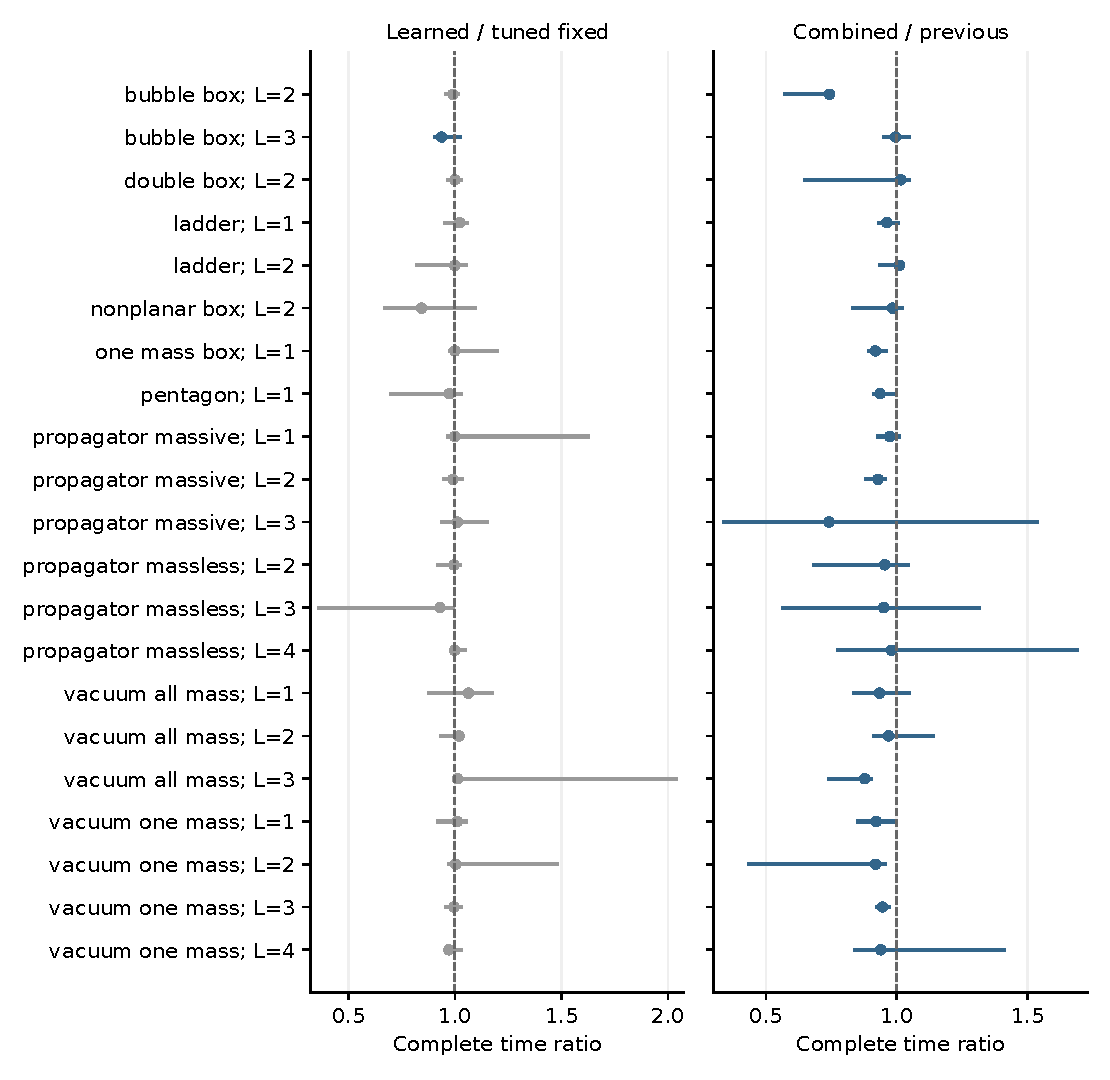
\includegraphics[width=\linewidth]{paper_figures/family_cost.pdf}
\caption{The learned and combined comparisons answer different questions. Points show complete-time ratios, horizontal lines show paired-repetition intervals, and the dashed line marks equal time. Gray points in the left panel have no changed model choice and show timing variation between identical actions. Each interval describes timing variation for the fixed measured workload. It does not describe all possible integrals of that family.}
\label{fig:family-cost}
\end{figure}\FloatBarrier

\subsection{Higher-loop preparation and exact scalar coverage}
The earlier allocation failures occur before a model selects seeds. The tested implementation creates three arrays indexed by sector, whose native size grows as $2^N+1$ for $N$ integral coordinates. Auxiliary numerator coordinates increase $N$ even when they never become denominators in any declared sector. We restrict these arrays and the sector-order table to the already admitted sector domain while keeping every relation and relative ordering in that domain. We also obtain the smallest nontrivial sector size by counting known trivial sectors, which avoids an exhaustive scan. Appendix~\ref{app:family-cost} gives the bound and its conditions. This is an exact storage change, and its gain is separate from the learned-choice comparison above.

The storage test retains 16 predefined requests and their full outcomes: 5 complete comparisons, 1 checked bounded reduction with an incomplete allocation control, 9 incomplete reference calculations, 1 incomplete independent reference check. The new calculation first discovers a basis and then checks it with increased numerator bounds and a different ordering. Where both storage methods complete, three repeated reductions compare coefficients and times in that common basis. A native allocation failure has no finite completion time and therefore supplies no finite speedup ratio. The detailed notes and evidence retain each failed request. A completed 64-bit reference whose enlarged check reaches the initial 60-second budget receives one 180-second check attempt. The increased numerator bound, changed ordering, exact comparison, and memory and storage limits remain unchanged; the initial failure remains in the evidence. Application timing retains its original budget.

A separate scalar test uses the full scalar-product coordinate representation at every loop order from one through twelve. All twelve batches pass the independently implemented raising recurrence of Appendix~\ref{app:extended-coverage}, with three targets per batch. Auxiliary powers remain zero. This extends the admitted representation of the exact scalar formula, including coordinate counts above the native interface limit. It establishes neither general twelve-loop native IBP reduction nor a twelve-loop learned gain.

The measured family ratios determine where the new choices help. Some families retain fixed or previous choices, and some larger calculations remain limited by preparation or algebra. These results do not establish a learned speedup for every integral type or every loop order.
\paragraph{Wider ordering representation.} The separate 128-bit test retains 16 predefined requests: 4 complete comparisons, 9 incomplete reference calculations, 3 incomplete independent reference checks. Both allocation methods use the wider representation. It addresses the ordering-label capacity and leaves coefficient arithmetic unchanged. The native coordinate limit and the cost of preparing IBP polynomials still apply.

\begin{table}[!htbp]\centering\small
\caption{Exact sector-storage checks with a common weight width in each pair. Times are median complete seconds; memory is peak process-tree resident memory in MiB. An incomplete native run has no finite time ratio. Only rows with a checked bounded reduction appear here; all other requests remain in the reported outcome counts.}
\begin{tabular}{@{}lrrrrr@{}}\toprule Family and loops & Bits & Native s & Bounded s & Native MiB & Bounded MiB\\\midrule
ladder L2 & 64 & 6.571 & 6.156 & 57.9 & 64.3\\
propagator massive L2 & 64 & 0.823 & 0.797 & 20.7 & 20.7\\
vacuum all mass L3 & 64 & 1.082 & 1.074 & 21.4 & 21.3\\
vacuum all mass L5 & 64 & incomplete & 45.218 & 142.3 & 168.7\\
vacuum one mass L3 & 64 & 0.742 & 0.737 & 20.0 & 20.2\\
vacuum one mass L5 & 64 & 11.099 & 10.321 & 132.6 & 110.9\\
ladder L2 & 128 & 6.802 & 6.366 & 105.3 & 77.5\\
propagator massive L2 & 128 & 0.795 & 0.785 & 20.9 & 20.8\\
vacuum all mass L3 & 128 & 1.097 & 1.080 & 22.0 & 21.8\\
vacuum one mass L3 & 128 & 0.761 & 0.739 & 20.8 & 20.5\\
\bottomrule\end{tabular}\end{table}\FloatBarrier
The vacuum all mass L5 batch contains 3 targets, including 1 nontrivial reductions in a reference basis of 32 integrals.
The vacuum one mass L5 batch contains 3 targets, including 2 nontrivial reductions in a reference basis of 1 integral.
\subsection{The final combined application}
We then combine the frozen models with an exact route selected from the separate storage validation. Low-loop bounded storage requires a measured gain of at least 3\% before deployment. For higher-loop cases that complete with wider weights, validation chooses the faster complete allocation method. Each selected route must also pass a complete application check. Other inputs keep the previous exact executable. The fitted model parameters remain unchanged. For deployment, the confirmation measurements also distinguish the dotted and mixed target patterns. A pattern uses the new learned choice only if its confirmation median is at least 3\% below both the fixed control and the previous application. This selects the mixed three-loop bubble-box pattern and retains the previous route for its dotted counterpart. We freeze this gate before the final test. A second matched comparison reruns the native control, previous application, fixed choice with validation-selected exact routes, learned choice with validation-selected exact routes, and final combined application. It uses a fresh reserved profile, $h=1151$, with the same graph and target construction and five rotated fresh-process repetitions. Each new request receives an independently discovered and checked master basis. This stage measures the combination directly; it does not multiply gains from separate experiments.

The final grid contains 44 batches, of which 41 give matched nontrivial reductions, 3 lack a checked reference, and 0 have application-failure records. Native and previous application totals are 66.045 and 58.729 seconds. The fixed and learned choices with validation-selected exact routes take 57.067 and 56.576 seconds, while the final combined application takes 56.461 seconds. The isolated learned-to-fixed ratio is 0.991, with interval [0.954, 1.019]. The final-to-previous ratio is 0.961, with interval [0.934, 1.021]. The final-to-native ratio is 0.855.

Bounded storage acts in 4 matched final batches; the other matched batches retain the previous storage route. The common reference construction takes 123.958 seconds and its independent checks take 330.029 seconds. Including reference construction gives 182.687 seconds for the previous two-stage workflow and 180.419 seconds for the final two-stage workflow.

The target-pattern gate activates on 1 matched batch. In this subset, the learned-to-fixed ratio under the same exact route is 0.839, with interval [0.780, 0.841]. The final-to-previous ratio is 0.826. The learned-to-native ratio is 1.006, with interval [0.931, 1.023]. Thus a gain against the tuned fixed control does not establish a gain against native bounds. This small subset measures the new model's deployed domain and does not establish transfer to other graph structures.

The summed median numbers of generated IBP equations in this subset are 26,095 for the fixed control and 19,153 for the learned choice, including recovery attempts. Native bounds generate 19,153 equations. For this mixed target batch, the model selects the native numerator-rank bound with relaxed truncation. This avoids the extra numerator-rank seeds in the family-wide fixed setting. These counts explain equation-generation work and do not count every algebraic operation.

All matched final outputs pass 12475 coefficient-pair checks. This comparison includes both the exact changes and the validation-selected application, while its learned-to-fixed control isolates the model's extra contribution.

\begin{table}[!htbp]\centering\small
\caption{Final combined comparison. Both learned and fixed controls use the same validation-selected exact route. The final application also retains exact scalar formulae and validated previous choices. The Changed column counts model decisions that differ from the fixed action.}
\label{tab:family-combined}
\begin{tabular}{@{}lrrrr@{}}\toprule
Family and loops & Batches & Changed & Learned/fixed & Final/previous\\\midrule
bubble box L2 & 2 & 0 & 1.179 & 0.613\\
bubble box L3 & 2 & 1 & 0.929 & 0.922\\
double box L2 & 2 & 0 & 1.025 & 0.981\\
ladder L1 & 2 & 0 & 1.029 & 0.871\\
ladder L2 & 2 & 0 & 1.043 & 1.068\\
nonplanar box L2 & 2 & 0 & 0.981 & 0.988\\
one mass box L1 & 2 & 0 & 1.017 & 1.010\\
pentagon L1 & 2 & 0 & 1.127 & 0.945\\
propagator massive L1 & 2 & 0 & 1.104 & 1.115\\
propagator massive L2 & 2 & 0 & 1.104 & 0.986\\
propagator massive L3 & 2 & 0 & 0.951 & 0.767\\
propagator massless L2 & 2 & 0 & 1.042 & 0.989\\
propagator massless L3 & 2 & 0 & 0.893 & 1.065\\
propagator massless L4 & 1 & 0 & 0.857 & 1.215\\
vacuum all mass L1 & 2 & 0 & 0.901 & 0.906\\
vacuum all mass L2 & 2 & 0 & 1.026 & 1.192\\
vacuum all mass L3 & 2 & 0 & 0.825 & 0.965\\
vacuum one mass L1 & 2 & 0 & 0.928 & 0.941\\
vacuum one mass L2 & 2 & 0 & 1.010 & 0.996\\
vacuum one mass L3 & 2 & 0 & 1.003 & 0.853\\
vacuum one mass L4 & 2 & 0 & 0.968 & 0.966\\
\bottomrule\end{tabular}\end{table}
\begin{figure}[!htbp]\centering
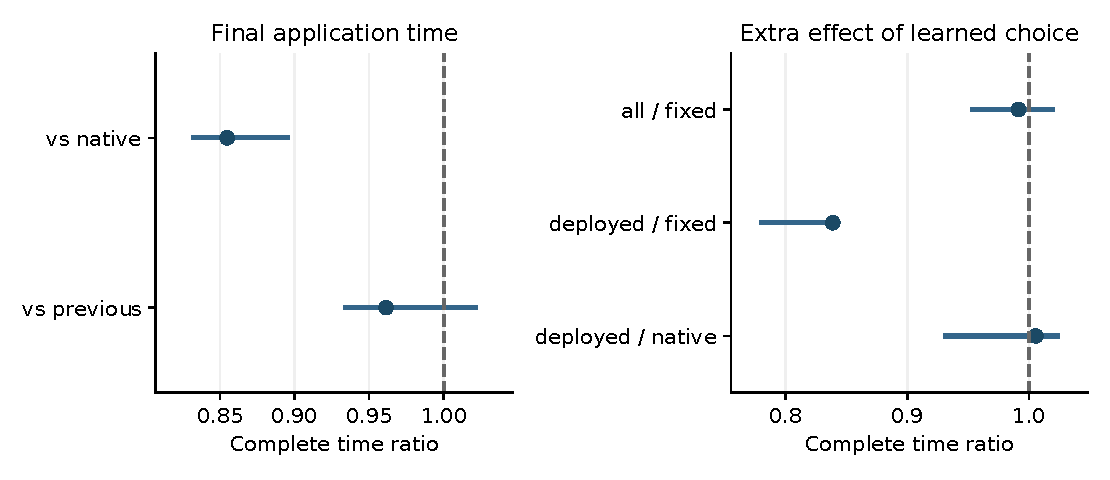
\includegraphics[width=\linewidth]{paper_figures/family_combined.pdf}
\caption{The final comparison separates complete application time from the extra effect of learned seed choices. The right panel compares the learned choice with fixed and native controls under the same exact route. The deployed subset contains the target pattern selected before testing, on which the model changes the seed action. Inactive domains use identical actions and contribute run variation to the all-matched comparison. Points show ratios and lines show paired-repetition intervals; the two horizontal scales resolve their different magnitudes.}
\label{fig:family-combined}
\end{figure}\FloatBarrier

\section{An exact higher-loop specialization alongside the learned method}
\label{sec:banana}
The learned choices above apply to the physical structures represented in their training and validation data. A useful reduction workflow can also use a proved integral identity when the requested family permits one. We implement this choice for massless two-point banana integrals, which have two vertices connected by $L+1$ massless lines at $L$ loops. Repeated one-loop convolution gives their coefficients directly~\cite{Grozin2004Banana}. This saving comes from the analytic identity and is measured separately from the learned decisions.

Let $p$ be the external momentum, with $p^2\ne0$, and let the physical denominators be $\ell_1^2,\ldots,\ell_L^2$ and $(p-\sum_j\ell_j)^2$. Each denominator has a positive integer power $a_i$. There are no numerator insertions in this specialization. Define $n=L+1$, $b_i=a_i-1$, $K=\sum_i b_i$, and the corner integral $M_L=B_L(1,\ldots,1)$. Appendix~\ref{app:banana} defines the measure and derives
\begin{equation}
 B_L(\boldsymbol a)=
 \frac{(n-Ld/2)_K(n+1-nd/2)_K}
 {(p^2)^K\prod_{i=1}^{n}(2-d/2)_{b_i}b_i!}\,M_L,
 \label{eq:banana-main}
\end{equation}
where $(z)_k=\prod_{j=0}^{k-1}(z+j)$ and $(z)_0=1$. Thus all scalar targets in this class have rational reduction coefficients in $d$ and $p^2$.

Before applying Eq.~\eqref{eq:banana-main}, the workflow checks the propagator momenta, zero masses, nonzero external squared momentum, and allowed indices. It forms and cancels exact linear factors in $d$. Other families pass to the native Kira workflow with the frozen batch and equation choices. Both the ML-enabled and ML-disabled comparison paths use the same analytic identity. The identity therefore contributes no saving to the reported ML comparison.

\subsection{Checks and measured time}
The first native comparison asks Kira to use the corner master with seed limits set directly by the targets. It completes the one-loop requests and fails in eight higher-loop requests. These failures include rejection of the supplied basis and an allocation failure during topology preparation. We retain all of them, then compare four fixed seed choices on a separate development point and freeze the fastest successful choice for each loop count and kinematic form. A new point supplies the matched comparison in Table~\ref{tab:banana}. Appendix~\ref{app:banana} gives the seed definitions and repetitions.

The follow-up completes 9 matched requests and leaves 1 request without a completed comparison. Six-loop development reports allocation failures during topology preparation under the imposed memory limit. Since no fixed seed choice passes, the six-loop reserved request does not run and receives no timing ratio. The completed requests check 81 native coefficients exactly. The complete-time speedup ranges from 21.3 to 357.8 times across the completed requests. Both paths include an exact coefficient check, and the direct path also includes its domain check. These timings exclude shared Python imports.
\begin{table}[!htbp]\centering\small
\caption{Complete times in seconds for the defined scalar banana targets. Native uses the development-selected fixed seeds with all ML disabled. Direct uses the proved formula. Each native time is the median of three repetitions.}
\label{tab:banana}
\begin{tabular}{@{}llrrr@{}}\toprule
Loops & $p^2$ & Native & Direct & Speedup\\\midrule
1 & Rational & 0.4223 & 0.0067 & 62.8$\times$\\
2 & Rational & 0.4425 & 0.0194 & 22.8$\times$\\
3 & Rational & 0.5373 & 0.0218 & 24.7$\times$\\
4 & Rational & 1.4625 & 0.0249 & 58.8$\times$\\
5 & Rational & 8.7544 & 0.0245 & 357.8$\times$\\
1 & Symbolic & 0.4693 & 0.0081 & 58.0$\times$\\
2 & Symbolic & 0.4966 & 0.0233 & 21.3$\times$\\
3 & Symbolic & 0.5555 & 0.0246 & 22.6$\times$\\
4 & Symbolic & 1.4615 & 0.0243 & 60.2$\times$\\
\bottomrule\end{tabular}\end{table}
\begin{figure}[!htbp]\centering
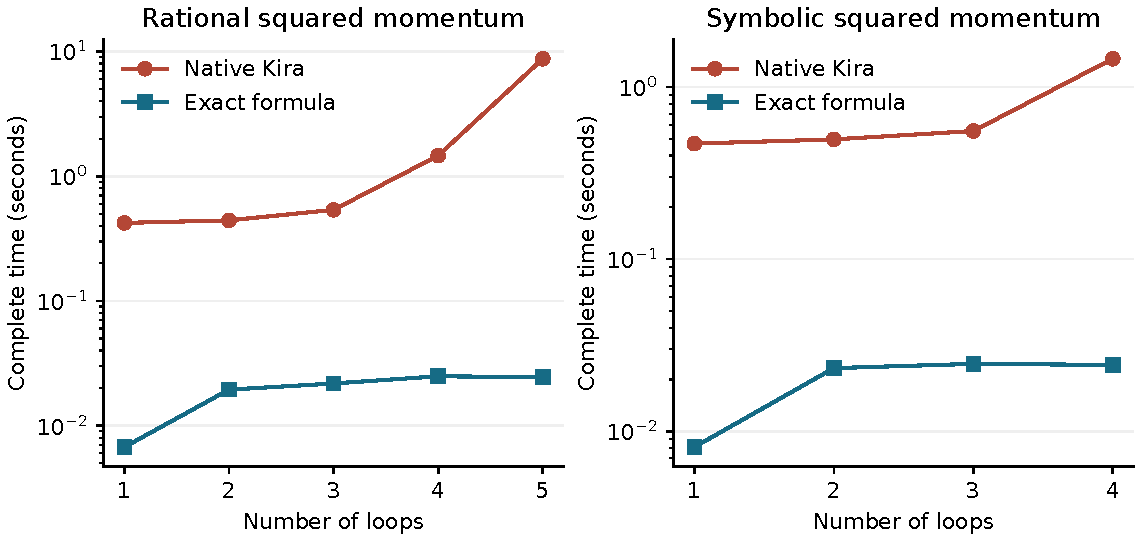
\includegraphics[width=\linewidth]{paper_figures/massless_banana_times.pdf}
\caption{The direct coefficient formula avoids the native equation system for the displayed scalar family. Times include exact coefficient checks. The logarithmic time axis shows both methods, and only completed native comparisons appear. These are analytic gains, separate from ML.}
\label{fig:banana}\end{figure}\FloatBarrier

An additional 240 numerical checks compare the finite rational formula with the uncancelled Gamma-function expression at one through twelve loops and at 16, 24, and 32 loops. They use 70-digit arithmetic at two noninteger dimensions. The general derivation supports this scalar family at every positive loop count; the numerical checks test its implementation at the stated counts. General higher-loop scattering remains outside this analytic specialization.

A separate test starts a new application process for each request. All 48 executions use the combined routing interface, and every successful output passes an exact check. It also passes 49 domain checks. The four analytic requests use one, four, eight, and twelve loops; their summed median application time is 0.6458 seconds. The same formula serves both comparison paths. The 4 matched native requests take 38.161 seconds with the frozen learned workflow and 38.318 seconds with the separately tuned ML-disabled workflow. These native requests repeat the predeclared application subset of the batch study, so they test integration and startup rather than new physical coverage.

The new seed-bound study in Section~\ref{sec:learned-bounds} isolates a learned choice with all earlier models disabled. On 68 matched nontrivial batches, complete application time changes from 164.926 seconds under native bounds and 119.717 seconds under tuned fixed settings to 119.081 seconds with the new model. This gives 27.8\% less time than native bounds and 0.5\% less time than the tuned fixed control. The comparison includes model loading, native IBP generation, exact reduction, coefficient checks, and recovery, with a supplied basis. It uses known structures at one through four loops and separate rational profiles; the additional saving over tuned fixed settings remains within timing variation.
% END CURRENT WORKFLOW UPDATE
\clearpage
\renewcommand{\refname}{Citations}
% BEGIN CURRENT WORKFLOW UPDATE
\appendix
\renewcommand{\thesection}{A\arabic{section}}
\renewcommand{\theHsection}{appendix.\arabic{section}}
\section{Integral families for the native cost comparisons}
\label{app:families}
The denominator convention is $D_i=q_i^2-m_i^2+\mathrm{i}0$, with the measure in Eq.~\eqref{eq:family}. This appendix collects the ordered momenta used by the later cost studies so that the notes specify their physical inputs independently of the companion paper. Appendix~\ref{app:adaptive} gives the masses, kinematic profiles, and target indices for the new comparisons. Appendix~\ref{app:higher-scattering} adds the connected higher-loop scattering families.

The sunrise uses
\begin{equation}
\boldsymbol q_{\rm S}=(\ell_1,\ell_2,p-\ell_1-\ell_2,p-\ell_1,p-\ell_2).
\end{equation}
Its first three entries are physical denominators and its last two entries are auxiliary. Their indices remain nonpositive.

\subsection{Native multiloop families}

The sunrise comparisons allow independent masses on the same three physical propagators. The other native comparison families use
\begin{align}
 \boldsymbol q_{\rm DB}={}&(\ell_1,\ell_1-p_1,\ell_1-p_1-p_2,
 \ell_2,\ell_2-p_1-p_2,\ell_2-p_1-p_2-p_3,\nonumber\\
 &\ell_1-\ell_2,\ell_1-p_3,\ell_2-p_1),\\
 \boldsymbol q_{\rm V}={}&(\ell_1,\ell_2,\ell_3,\ell_1-\ell_2,
 \ell_2-\ell_3,\ell_1-\ell_3),\\
 \boldsymbol q_{\rm L}={}&(\ell_1,\ell_1-p,\ell_2,\ell_2-p,\ell_3,
 \ell_3-p,\ell_1-\ell_2,\ell_2-\ell_3,\ell_1-\ell_3).
\end{align}
The double box has two loops and seven physical denominators; its last two entries are auxiliary. The vacuum has three loops and six physical denominators. The ladder has three loops and eight physical denominators; its last entry is auxiliary. Auxiliary indices remain nonpositive. The massless double box has $p_i^2=0$ and uses $2p_1\cdot p_2=s$, $2p_1\cdot p_3=t$, $2p_2\cdot p_3=-s-t$. This local definition of $t$ differs from the initial box convention because the routing differs.


\subsection{Scattering structures and symbolic invariants}

The massless nonplanar box uses the routing of Ref.~\cite{KiraOriginal}:
\begin{align}
 \boldsymbol q_{\rm NP}={}&(\ell_1,\ell_2,p_1-\ell_1,p_2-\ell_2,
 p_1+p_2-p_3-\ell_1,\nonumber\\
 &p_1-\ell_1+\ell_2,p_1-p_3-\ell_1+\ell_2,
 \ell_1-p_3,\ell_2-p_1-p_2).
\end{align}
The first seven entries are physical propagators, and the final two are auxiliary entries. Here $p_1^2=p_2^2=p_3^2=(p_1+p_2-p_3)^2=0$, $s=(p_1+p_2)^2$ and $t=(p_1-p_3)^2$. Expanding these squares gives $2p_1\cdot p_2=s$, $2p_1\cdot p_3=-t$ and $2p_2\cdot p_3=s+t$.

The massless pentagon uses $\sum_{i=1}^5p_i=0$, $p_i^2=0$ and
\begin{equation}
 \boldsymbol q_{\rm P}=(\ell,\ell-p_1,\ell-p_1-p_2,
 \ell-p_1-p_2-p_3,\ell-p_1-p_2-p_3-p_4).
\end{equation}
All five denominators are physical. The independent invariants are $(s_{12},s_{23},s_{34},s_{45},s_{51})$, where $s_{ij}=(p_i+p_j)^2$. Squaring $p_1+p_2+p_3=-(p_4+p_5)$ gives $2p_1\cdot p_3=s_{45}-s_{12}-s_{23}$; the other nonadjacent products follow by cyclic relabelling. The box with an external virtuality uses $\boldsymbol q=(\ell,\ell-p_1,\ell-p_1-p_2,\ell-p_3)$, $p_1^2=p_2^2=p_3^2=0$, and $v=(p_1+p_2-p_3)^2$. With the nonplanar convention for $s,t$, expanding $v$ gives $2p_2\cdot p_3=s+t-v$.

\section{Learning the cost of a complete reduction}
\label{app:workflow}
This appendix defines the complete-time prediction problem, derives the fitted models, and specifies the physical inputs used in Section~\ref{sec:workflow}. The cost model receives a feature vector $\boldsymbol f_c$ for target batch $c$.
Its entries are the number of loops, external momenta, inverse propagators,
physical propagators and symbolic invariants; $\log(1+n_c)$, where $n_c$ is
the number of targets; the maximum dot count, maximum numerator rank, mean dot count and mean numerator rank;
the number of target sectors; and seven indicators for the graph structures.
An indicator is one for its graph and zero for the other graphs.
Together these quantities give eighteen inputs, all available from the requested targets and family before reduction.

For an index vector $\boldsymbol a$, define
\begin{equation}
 r(\boldsymbol a)=\sum_i\max(a_i,0),\qquad
 s(\boldsymbol a)=\sum_i\max(-a_i,0),\qquad
 q(\boldsymbol a)=\sum_i\max(a_i-1,0).
\end{equation}
Here $r$ is the positive index sum, $s$ is the numerator rank, and $q$ is
the number of extra denominator powers, called dots. These definitions
follow directly by counting the denominator and numerator factors.
The initial bounds $B_c=(r_c,s_c,q_c)$ are the componentwise maxima over
the targets. The trial seed regions use $B_c$, $B_c-(1,1,1)$,
$B_c-(1,0,1)$, or $B_c+(1,1,1)$. Negative bounds are set to zero.
The choices change the region in which equations are generated. Since a smaller region can omit required relations, every attempt must still pass the prescribed-basis check.

Let $t_{cj}$ be the median complete time of strategy $j$ on training batch
$c$, and let $t_{c0}$ be the time of the integrated native strategy.
The training response is
\begin{equation}
 y_{cj}=\log\frac{t_{cj}}{t_{c0}}.
 \label{eq:workflow-label}
\end{equation}
Each time includes unsuccessful attempts and the eventual successful fallback, so a strategy that omits necessary equations is penalized by the extra calculation. The logarithm preserves the ordering of positive time ratios; minimizing the response therefore also minimizes the complete time relative to the common baseline.

We fit constant, tree, linear and nearest-neighbour predictors of this
response. The constant predictor averages each strategy's training
responses. A tree splits the feature space and uses a constant vector
within each leaf, following regression-tree construction~\cite{CART1984}.
For a leaf containing training set $A$, minimizing
$\sum_{c\in A}(y_{cj}-v_j)^2$ gives
\begin{equation}
 \frac{\partial}{\partial v_j}
 \sum_{c\in A}(y_{cj}-v_j)^2
 =2|A|v_j-2\sum_{c\in A}y_{cj}=0,
 \qquad v_j=\frac{1}{|A|}\sum_{c\in A}y_{cj}.
\end{equation}
Each split minimizes the sum of squared errors over the seven strategies.
The tested maximum depths are two, four and six. Each depth is tested
with a minimum of either one or three training batches per child.

For the linear models, we first subtract the training mean of each feature and
divide by its training population standard deviation, computed with
divisor equal to the number of training batches. A constant feature uses
divisor one. Let $Z$ contain these standardized feature rows with a leading intercept column, and let $Y$ contain the responses.
Ridge regression minimizes
\begin{equation}
 J(W)=\|ZW-Y\|_F^2+\lambda\operatorname{tr}(W^TPW),
 \qquad P=\operatorname{diag}(0,1,\ldots,1).
\end{equation}
Here $W$ is the matrix of fitted coefficients, $\|\cdot\|_F^2$ is the sum
of squared matrix entries, and $P$ leaves the intercept unpenalized.
Differentiating each entry of $W$ gives
\begin{equation}
 \nabla_WJ=2Z^T(ZW-Y)+2\lambda PW=0,
 \qquad (Z^TZ+\lambda P)W=Z^TY.
\end{equation}
We solve this system for $\lambda=0.1,1,10$.

The nearest-neighbour models estimate a cost from similar training batches. Eligible neighbours must have the same graph, loop count, external-momentum count, propagator counts, and number of symbolic invariants. They choose up to two or four training batches with
the smallest squared distance in standardized features. The predicted
response is the mean of their response vectors. The leaf-mean derivative
above also derives this local constant estimate. If no eligible neighbour
exists, the predictor returns equal costs and the selector uses native
choices.

Let $j_*$ be the strategy with the smallest predicted logarithmic cost
$\widehat y_j(\boldsymbol f)$. Validation selects a margin
$\gamma\in\{0,0.05,0.15\}$, and the model chooses the strategy as follows:
\begin{equation}
 \widehat j(\boldsymbol f)=
 \begin{cases}
 j_*,&\widehat y_{j_*}(\boldsymbol f)<\widehat y_0(\boldsymbol f)-\gamma,\\
 0,&\text{otherwise}.
 \end{cases}
 \label{eq:workflow-choice}
\end{equation}
Subtracting the two predicted logarithmic costs shows that the condition
requires a predicted relative cost below $e^{-\gamma}$. Validation selects
the model and margin with the smallest geometric mean time ratio.
The selected settings remain fixed during reserved tests.
This finite comparison establishes the best measured candidate within
the study. It does not prove a globally optimal reduction strategy.

\subsection{Parameter points and target lists}
The comparison uses the sunrise, planar box, three-loop vacuum, three-loop ladder, nonplanar box, pentagon, and box with external virtuality, with the same denominator routings and kinematic conventions as the preceding tests. The definitions below specify the parameter values and target lists for each split. Let $h$ identify a rational
parameter profile. Training uses $h=41,42$, validation uses $h=43$, and
testing uses $h=44,45$. In a common squared-momentum unit, the sunrise has
squared masses $(2,7,11)$ and $p^2=-1009-12h$. The planar box has
$(s,t)=(-1009-12h,-1021-14h)$. The three-loop vacuum has squared masses
$(1,1,1,1,1,53+2h)$. The ladder keeps squared masses
$(1,0,0,0,0,0,0,0)$ and has $p^2=-1009-12h$.
The scattering assignments are
\begin{align}
 (s,t)_{\rm NP}&=(-113-18h,-127-10h),\\
 (s_{12},s_{23},s_{34},s_{45},s_{51})_{\rm P}
 &=(-11-20h,-13-20h,-17-20h,-19-20h,-23-20h),\\
 (s,t,v)_{\rm box}&=(-113-18h,-127-10h,-149-12h).
\end{align}
These assignments fix the rational parameter values in each profile while leaving the dimension symbolic. The additional symbolic batches instead retain all independent invariants of their scattering graph as symbols.

For the four earlier multiloop graphs, we retain the ordered target list
that starts with the corner, raises each physical denominator power once,
and then introduces each single auxiliary numerator. We repeat these
steps after removing one, two and three physical denominators, retain at
least two, and remove duplicates. Each rational profile supplies a
four-target batch and a batch of the first 32 targets, or all 21 targets
for the sunrise. The three scattering graphs use the same construction
with at most one removed denominator. Their larger batches have 32, 31
and 21 targets for the nonplanar box, pentagon and virtuality box.

For the symbolic nonplanar box and pentagon, training takes target entries
12--15, validation takes 16--19, and testing takes 20--23, with numbering
starting at zero. These lists do not overlap. For the symbolic virtuality
box, the respective single targets are $(3,1,1,1)$, $(1,3,1,1)$ and
$(1,1,3,1)$. These targets have two extra powers on one physical denominator.
The rational batches reuse target patterns at different parameter points.

The joint-request test uses the larger rational batch at $h=44$ for each
graph and the three symbolic test batches. The symbolic virtuality box
also includes $(1,1,1,3)$, so it can supply two disjoint requests. A group
of $n$ targets is divided after entry $\lfloor n/2\rfloor$, with the first
request containing that many entries. The two requests share the same family definition and are available together, and their union contains each target once. By linearity, selecting the corresponding target rows from the joint reduction returns the coefficients for each original request. This separation leaves every coefficient unchanged and requires no new integral identity. The test reuses reserved parameter points and keeps the learned
model fixed.

\subsection{Combining the measured times}
Let $m_{cj}$ be the median of the five test times for batch $c$ and
method $j$, and let method zero be its stated native control.
For graph $g$ with batch set $C_g$, we define
\begin{equation}
 R_{gj}=\exp\!\left[\frac{1}{|C_g|}
       \sum_{c\in C_g}\log\frac{m_{cj}}{m_{c0}}\right],
 \qquad
 R_j=\exp\!\left[\frac{1}{7}\sum_{g=1}^{7}\log R_{gj}\right].
\end{equation}
The logarithm of a product equals the sum of the logarithms, so each
expression is the corresponding geometric mean of the time ratios.
The second expression assigns equal weight to each graph even when the
numbers of batches differ. A ratio $R_j<1$ means less time. The percentage
saving is $100(1-R_j)$, and the reciprocal $1/R_j$ is the speedup.

For the descriptive intervals, we sample seven graph labels with
replacement, calculate their mean logarithmic ratio, and exponentiate.
We repeat this 10,000 times and report the 2.5th and 97.5th percentiles.
This procedure describes variation among the seven tested graphs.
It does not provide a population guarantee for other integral families.
The joint-request comparison uses the same calculation, with separate
native requests as its first control. Its parameter points overlap the
main reserved test, so it is an additional comparison on the same test
population.

\section{Separate cost models for each graph}
\label{app:type-specialists}
This experiment retains the seven denominator definitions and profile
formulas in Appendix~\ref{app:workflow}. Development uses profile $h=61$,
training uses $h=62,63$, validation uses $h=64$, and the reserved test uses
$h=65,66$. The dimension remains symbolic. Related target batches share
the same split, so their rational kinematic values cannot pass from the
training set into the reserved set. The graph structures and target
patterns occur in both sets.

Let $P$ be the number of physical propagators and let
$\boldsymbol b=(1,\ldots,1,0,\ldots,0)$ have $P$ entries equal to one.
Let $\boldsymbol e_j$ be the unit vector for index $j$. The first batch
contains $\boldsymbol b+2\boldsymbol e_j$ for
$j=1,\ldots,\min(P,3)$. Thus one denominator has power three in each target.
For the second batch, define the lower-sector corner
\begin{equation}
 \boldsymbol b^{\rm low}=
 \begin{cases}
 \boldsymbol b-\boldsymbol e_1,&P<5,\\
 \boldsymbol b-\boldsymbol e_1-\boldsymbol e_3,&P\geq5.
 \end{cases}
\end{equation}
Include this corner and up to three single-dot targets,
$\boldsymbol b^{\rm low}+\boldsymbol e_j$ with $b^{\rm low}_j=1$,
taking the first available indices in increasing order.
The third batch uses the original corner $\boldsymbol b$ and contains
$\boldsymbol b-2\boldsymbol e_j$ for the first three auxiliary entries,
or all auxiliary entries when fewer than three exist. When a family has no auxiliary entry, this construction
repeats the first batch and we remove the duplicate. These formulas define
the inputs; they do not infer their coefficients from the masters.

\subsection{The allowed changes to Kira}
For target batch $\mathcal T$ and a target $\boldsymbol a$, let $S(\boldsymbol a)=\{i:a_i>0\}$ be its
positive-index set. One strategy supplies only maximal target sectors:
\begin{equation}
 \mathcal S_{\rm max}
 =\{S(\boldsymbol a):\boldsymbol a\in\mathcal T,
 \ S(\boldsymbol a)\not\subsetneq S(\boldsymbol a')
 \text{ for every }\boldsymbol a'\in\mathcal T\}.
 \label{eq:type-sectors}
\end{equation}
Kira then includes their subsectors. To see why this is a useful candidate,
consider the shifted integrals produced by the IBP derivative. A raised
index $a_i+1$ carries a factor $a_i$, and the other shifts lower an index.
If $a_i=0$, the raising term vanishes; if $a_i<0$, raising it once leaves
it nonpositive. Thus an IBP equation seeded in one sector stays in that
sector or its subsectors. This observation does not prove that the
restricted pool contains every relation useful for a chosen master basis.
We therefore retain the basis check and full-sector fallback.

Another strategy uses Kira's numerator truncation~\cite{Kira3}. In a sector
with $t$ positive indices, Kira restricts the inherited numerator bound by
\begin{equation}
 s\leq\max(1,t-\tau+1,s_{\rm explicit}),
 \label{eq:type-truncation}
\end{equation}
where $\tau$ is the chosen integer cutoff and $s_{\rm explicit}$ is a
bound explicitly supplied for that sector. We test
$\tau=P-s_c$ and $\tau=P-s_c+1$, where $s_c$ is the largest target numerator
rank. The top-level sector retains its explicit target bound. The first
cutoff combined with maximal target sectors forms the deterministic
control. The development probes also test $\tau=P-s_c-1$.

The remaining choices use the original bounds $B_c$, the smaller bounds
$B_c-(1,0,1)$ with negative entries replaced by zero, the larger bounds
$B_c+(1,1,1)$, Kira integral ordering five~\cite{Kira12}, or the preceding
trained equation filter. Together these choices give nine strategies.
Before each attempt, every strategy enforces a nonempty seed region in
its declared top-level sectors. If $\mathcal S_0$ is that sector list and
$r_{\rm req}$ is the requested positive-index bound, the actual bound is
\begin{equation}
 r_{\rm run}=\max\left(r_{\rm req},\max_{S\in\mathcal S_0}|S|\right).
 \label{eq:type-valid-bound}
\end{equation}
Each positive index is at least one, so a seed in sector $S$ has
$\sum_{i\in S}a_i\geq|S|$. This proves the lower bound used in
Eq.~\eqref{eq:type-valid-bound}. The correction prevents an invalid
configuration from adding a failed startup to any method's cost.
Identical input configurations share one training or validation measurement.
If a proposed reduction fails, it retries with native choices at $B_c$
and then at $B_c+(1,1,1)$. The recorded cost includes every attempt.

\subsection{Fitting and selecting the models}
Each graph has its own predictors of
$y_{cj}=\log(t_{cj}/t_{c0})$, where $t_{cj}$ is the median complete cost of
strategy $j$ on batch $c$ and zero denotes native choices. The nine input
features are the target count; maximum dot count and numerator rank;
minimum and maximum positive-index counts; mean dot count and numerator
rank; number of maximal target sectors; and number of physical
propagators. These features use the requested indices and family
definition. They contain no reduced coefficients.

We fit ten candidates per graph: one constant predictor, trees of maximum
depth one, two and three, a bagged ensemble of sixteen depth-three trees,
ridge regressions with penalties $0.1,1,10$, and nearest-neighbour
predictors with one and three neighbours. Trees use squared-error splits
with at least one row in each child. Each ensemble tree receives a
bootstrap sample of the training batches and uses all features at each
split. This follows bootstrap aggregation~\cite{Breiman1996Bagging}.
For fitted trees $f_1,\ldots,f_{16}$, the ensemble prediction is
\begin{equation}
 \widehat y_j(\boldsymbol f)=\frac1{16}
 \sum_{b=1}^{16}f_{bj}(\boldsymbol f).
\end{equation}
This average also follows by minimizing
$\sum_b(f_{bj}(\boldsymbol f)-v_j)^2$ with respect to $v_j$, using the
leaf-mean derivative in Appendix~\ref{app:workflow}. That appendix derives
the ridge fit and the local-mean estimates used here. Neighbour distances
use the training standard deviations; a constant feature uses divisor
one. We use two timing repetitions for training and three for validation.
Within each batch comparison, every strategy uses the same computer.
Different training batches can use different computers, and the
training response normalizes each cost to its own batch baseline.

Validation considers decision margins $0,0.05,0.15$ in
Eq.~\eqref{eq:workflow-choice}. It chooses the candidate and margin with
the lowest complete cost separately for each graph. The controls are
native choices, the deterministic sector-and-truncation rule, and the
single strategy with the lowest geometric mean training cost for that
graph. A fixed strategy can include the older equation filter. We enable
the new model only when its validation cost ratio to the fastest control
is at most $0.95$. Otherwise, the route uses that control. This threshold
is a selection rule, not a significance test. Unknown graph structures
and features outside the fitted range use native choices.

The reserved comparison uses five repetitions of native choices, the
deterministic rule, the fixed strategy per graph, and the selected route.
The order rotates across batches and repetitions, giving every method
the same number of appearances in each run position over the full test.
Each run uses the same targets, prescribed basis, executable, and one
processor. All methods retain the preceding exact implementation
improvements, so the native control uses that same implementation with
native selection rules. Full time includes input preparation, prediction, native IBP
generation, exact reduction, coefficient checks, cleanup, and retries.
Offline fitting, reference discovery, and saving measurement records stay
outside the timer. Separate application checks receive the basis without
target coefficients and compare their answers only after completion.
The calling program and fitted parameters are loaded before the timing
trials, and each trial starts a fresh Kira process. The additional
application checks also record time with a newly started calling program;
they do not supply a matched speed comparison for that condition.

We combine five-run median ratios within each graph and then give the
seven graphs equal weight, as derived in Appendix~\ref{app:workflow}.
The aggregate intervals resample graph groups. Per-graph plot bars show
the range across the two reserved kinematic profiles. Two profiles do not
support a general significance claim for that integral type, so those
bars are reported as ranges.

\section{Selective seed expansion and exact basis completion}
\label{app:basis-completion}
The seed-expansion study asks whether a smaller first calculation and an exact conversion of its remaining integrals can be cheaper than one large reduction. It uses the seven families in Appendix~\ref{app:workflow} and the target definitions in Appendix~\ref{app:type-specialists}. Development
uses profile $h=71$, training uses $h=72,73$, validation uses $h=74$, and
the reserved test uses $h=75,76$. These are separate rational parameter
profiles. The graph structures and target index patterns occur in all
splits, and $d$ remains symbolic.

\subsection{Changing individual seed bounds}
The bounds $B_c=(r_c,s_c,q_c)$ retain the definitions in
Appendix~\ref{app:workflow}: $r_c$ bounds the sum of positive indices,
$s_c$ bounds the numerator rank, and $q_c$ bounds the number of extra
denominator powers. Each component starts from the largest value among
the requested targets. We first enforce the sector lower bound in
Eq.~\eqref{eq:type-valid-bound}. The six new direct reductions use
\begin{equation}
 B_c+\boldsymbol\delta,\qquad
 \boldsymbol\delta\in\{(1,0,0),(0,1,0),(0,0,1),
                         (1,0,1),(1,1,0),(0,1,1)\}.
 \label{eq:basis-deltas}
\end{equation}
For a seed with $t$ positive indices, summing $a_i=1+(a_i-1)$ over those
indices gives $r=t+q$. The positive-index and extra-power limits can
therefore overlap, and different requested triples can give the same
seed region after all limits are applied. The labels therefore identify requested limits rather than necessarily distinct equation sets. Their purpose is to allow selective expansion, such as requesting more numerator identities without also increasing both denominator limits. Sufficiency remains a property to check for the resulting system. Each direct
reduction keeps the prescribed-basis check described in Ref.~\cite{Kira3}.
If it fails, the calculation calls the preceding fixed graph-specific
method and includes both attempts in its time.

\subsection{Completing a temporary basis}
We also test two ways to complete a smaller reduction. The first stage
uses $B_c$ and supplies the preferred masters, while allowing Kira to
return additional integrals. Kira supports this behaviour when its early
master-basis check is disabled~\cite{Kira3}. Let $M_m$ denote prescribed
masters and let $U_u$ denote additional integrals that remain in the
first-stage output. For target $I_t$, this stage returns exact relations
\begin{equation}
 I_t=\sum_m A_{tm}M_m+\sum_u C_{tu}U_u.
 \label{eq:basis-intermediate}
\end{equation}
Here $A_{tm}$ is the coefficient of prescribed master $M_m$, and
$C_{tu}$ is the coefficient of unresolved integral $U_u$. These
coefficients are rational functions of the kinematics and $d$.
The integrals $U_u$ are unresolved in the smaller first-stage system and need not be independent masters of the full family. Their index vectors define the targets of the second reduction, allowing that calculation to focus on the integrals that actually remain. That request uses its own componentwise target bounds
plus $(1,1,1)$ and again supplies the prescribed basis. One candidate uses
the maximal sectors of the $U_u$ and their subsectors; the other keeps the
original top-level sectors. Both retain the positive-index lower bound.

If the second reduction succeeds, it gives
\begin{equation}
 U_u=\sum_m H_{um}M_m.
 \label{eq:basis-bridge}
\end{equation}
The coefficient $H_{um}$ multiplies master $M_m$ in the reduction of $U_u$.
Substitution of Eq.~\eqref{eq:basis-bridge} into
Eq.~\eqref{eq:basis-intermediate} yields
\begin{align}
 I_t
 &=\sum_m A_{tm}M_m+\sum_u C_{tu}\sum_mH_{um}M_m\\
 &=\sum_m\left(A_{tm}+\sum_uC_{tu}H_{um}\right)M_m.
 \label{eq:basis-compose}
\end{align}
The final coefficient matrix is therefore $A+CH$. Computing its entries exactly in the rational-function field, cancelling common factors, and checking the final integral labels gives a reduction in the prescribed basis. When either reduction fails, the preceding method supplies a full
fallback. If no additional integral occurs, the second reduction is
unnecessary. All basis conversion and fallback costs enter the timer.
Independent reference coefficients check the final result only; the
policy and the two reduction stages do not receive them.

\subsection{Training, model selection, and comparison}
The development set compares the preceding method, six direct expansions,
and two basis-completion choices. We retain the preceding method and each
case's fastest candidate when it lowers that case's complete time by at
least ten percent. This rule selects candidates before training and does
not inspect reserved data.

We then fit the ten model types and nine target features defined in
Appendix~\ref{app:type-specialists}, separately for each graph. The new
response is $\log(t_{cj}/t_{c\mathrm{prev}})$, so it directly measures
improvement over the preceding method. Here $t_{cj}$ is the median complete
time of candidate $j$ on batch $c$, and $t_{c\mathrm{prev}}$ is the
corresponding time of the preceding method. Two repetitions supply each
training label, and three repetitions supply each validation cost. A
fixed strategy minimizes geometric mean training time for each graph.
Validation first selects the faster control between that fixed strategy
and the preceding method. It then tests the fitted predictors at margins
$0,0.05,0.15$ and enables one only when it lowers the control's validation
time by at least five percent. The fitting formulas and their derivations
remain those in Appendices~\ref{app:workflow} and
\ref{app:type-specialists}.

The fixed control may call the learned method retained from the preceding study. Its purpose is to isolate the benefit of the new choice among candidates while preserving the earlier improvements in every method.

The chosen graph policy and candidate set are fixed before the reserved
tests. Inputs with another graph structure or target features outside the
training range use the preceding method. That method retains its own
native fallback. Each reserved batch compares native choices, the
preceding method, the new fixed strategy, and the selected new method on
the same computer. Five repetitions use a rotating order. All methods
use the same executable and exact final coefficient checks. The time
includes preparation, prediction, Kira, any basis conversion, checking,
cleanup, and every retry. Offline training, independent reference
generation, and writing benchmark records remain outside these times.
The selection program and fitted parameters are loaded
before these trials; each attempt starts a fresh Kira process. Separate
application tests start a new caller and supply only the targets, family,
and prescribed basis. They check the coefficients after the reduction.

We first take the median time for each batch and method, then combine
ratios within each graph and give all seven graphs equal weight. The
geometric-mean derivation in Appendix~\ref{app:workflow} also applies here.
Descriptive aggregate intervals resample the seven graph groups. The
per-graph bars show the range over the two reserved parameter profiles.
These ranges describe the tested profiles and do not establish a gain
for all integrals with the same graph.

\section{Learned choices of integral and propagator order}
\label{app:ordering-policy}
This appendix specifies the ordering choices and explains why consistent relabelling leaves the integrals unchanged. The comparison uses the family definitions and target patterns in Appendix~\ref{app:type-specialists}. We use parameter profile 81 for
development, profiles 82 and 83 for training, profile 84 for validation,
and profiles 85 and 86 for the reserved comparison. Each profile uses
the rational parameters defined there, while the dimension $d$ remains
symbolic. These are new parameter values of known graphs and target
patterns.

\subsection{What the choice changes}
Kira provides eight integral orderings~\cite{Kira12}. Order one treats
numerator powers as simpler than extra denominator powers, called dots;
order two reverses that preference. Orders three and four first compare
their sum and then favour numerator powers or dots, respectively.
Orders one through four compare sectors by sector number. Orders five
through eight use the corresponding index rules but first compare the
number of positive indices and favour subsectors of the declared top
sectors. We also test the four automatic propagator permutation schemes
of Kira~\cite{Kira3}. The final coefficients use the original index
convention in every comparison.

The development candidates retain the preceding method, test each integral
order from two through eight with propagator scheme one, and test
propagator schemes two through four with integral order one. These are
eleven initial choices. For each development batch, we also combine its
fastest nondefault integral order with its fastest nondefault propagator
scheme and time that pair. This adds one development calculation per
batch. The preceding seed policy remains active in each
new choice. It can use truncation, selected seed bounds, or temporary-basis
completion as defined in the preceding appendices. A changed ordering is
applied to each Kira attempt in that method. If it fails to reduce to the
prescribed basis, we repeat the preceding method with its original settings.
Both attempts enter the recorded time. This finite comparison does not
search every joint ordering or every possible elimination sequence.

To see why changing labels preserves an integral, let $\pi$ be a
permutation of the $N$ propagator positions. Set
$D'_i=D_{\pi(i)}$ and $a'_i=a_{\pi(i)}$. Reindexing the product gives
\begin{equation}
 \prod_{i=1}^{N}(D'_i)^{-a'_i}
 =\prod_{i=1}^{N}D_{\pi(i)}^{-a_{\pi(i)}}
 =\prod_{j=1}^{N}D_j^{-a_j},
 \qquad I_{D'}(\mathbf a')=I_D(\mathbf a).
 \label{eq:order-relabel}
\end{equation}
Here $I_D$ denotes the integral defined by propagators $D_i$. Since the relabelling also leaves the measure unchanged, it preserves the integral. Changing the priority of integrals instead changes the sequence in which Kira solves the IBP equations. If $A\mathbf I=0$ denotes
those equations and $P$ is the permutation matrix that reorders the integral columns, then
\begin{equation}
 \mathbf J=P\mathbf I,\qquad
 AP^{-1}\mathbf J=A\mathbf I=0.
 \label{eq:order-system}
\end{equation}
The permutation therefore represents the same equations with a different column order. In a finite calculation, however, the ordering can also affect which equations are selected, so the equivalence of representations does not replace the checks of completeness and exact output coefficients.
We require every target to reduce to the prescribed master basis and
compare every output coefficient with an independent expanded-seed
reduction. The predictor receives neither those coefficients nor the
reference reduction steps.

\subsection{Training, validation, and timing}
For each development batch, we retain the fastest candidate if its full
time is at least ten percent below the preceding method. We also retain
the preceding method. The resulting candidate set is fixed before training.
We fit the same ten predictor types per graph as in
Appendix~\ref{app:basis-completion}, using the same nine features and
complete-time log-ratio labels. Training has two measurements per
candidate and batch; validation has three. Validation chooses a fixed
control and enables a predictor only when it saves at least five percent
against that control. We freeze the models, controls, and selection requirements before
using the reserved profiles.

Each application selects its ordering before Kira creates integral weights
and generates equations. The prediction is made once per requested batch.
The selected method retains the earlier seed policy, and Kira performs all
algebraic operations. The decision selects a setting for the complete reduction before it starts. Kira continues to choose individual row operations, as required by the earlier row-model comparison.

The reserved comparison measures native choices, the preceding method,
the training-selected fixed setting for each graph, and the new selected
method. It uses five repetitions with rotating execution order. The same
worker handles all methods for each batch. The timer includes prediction,
input preparation, native equation generation, exact algebra, basis
conversion where needed, coefficient checks, fallback, and cleanup.
The caller and models are already loaded, and each attempt starts a new
Kira process. Offline development, reference construction, training, and
record writing are excluded. Additional applications receive the target
indices and master basis without reference coefficients. Their results
are checked independently after the reduction.

\section{Selecting the number of Kira workers}
\label{app:thread-policy}
The worker-count study retains the seed strategy from Section~\ref{sec:basis-completion} and varies only the number of Kira workers used for a requested batch. The families and target patterns are those in Appendix~\ref{app:type-specialists}. Parameter profile 91 supplies the
development test, profiles 92 and 93 supply training, profile 94 supplies
validation, and profiles 95 and 96 supply the reserved comparison.
The dimension remains symbolic. Target patterns overlap across these
sets; the rational kinematic values differ.

\subsection{Choices and exactness}
The preceding learned method chooses seed bounds and can reduce through
a temporary basis. We retain that method and let a new policy choose
one, two, or four Kira workers for each requested batch. The choice
applies to each Kira attempt, including a temporary-basis conversion.
Kira supports parallel symbolic reduction~\cite{KiraOriginal}. Changing the worker count changes how operations are scheduled, while each operation continues to use exact rational arithmetic. Every output must reach the
prescribed master basis and agree with an independent expanded-seed
reduction. If a new choice fails, its time and the repeat with the
preceding one-worker method both enter the complete time.

Let $A\mathbf I=0$ denote the IBP system. An exact elimination step
left-multiplies it by an invertible elementary matrix $E$, so
\begin{equation}
 A\mathbf I=0\quad\Longleftrightarrow\quad
 EA\mathbf I=0.
 \label{eq:thread-row-equivalence}
\end{equation}
Multiplication by $E$ proves the forward implication, and multiplication by $E^{-1}$ proves the reverse. Repeating valid steps therefore preserves the system, provided parallel execution respects their dependencies. Kira manages those dependencies through its existing workers, while the predictor sets only their number.
This argument preserves relations but does not prove that a finite seed
set is sufficient. The basis and coefficient checks therefore remain
part of every measured reduction.

\subsection{Cost labels and selection}
Write $x$ for the nine target features defined in
Appendix~\ref{app:basis-completion}, and $q\in\{1,2,4\}$ for the worker
count. For training batch $b$, let $t_{b,q}$ be the median complete time of
two measurements. The training label is
\begin{equation}
 y_{b,q}=\log(t_{b,q}/t_{b,1}).
 \label{eq:thread-label}
\end{equation}
Because the logarithm is strictly increasing and $t_{b,1}>0$ is common
to all choices for that batch, minimizing this label also minimizes
$t_{b,q}$. We fit the same ten predictor types per graph as in
Appendix~\ref{app:basis-completion}. They include constants, trees,
bagged trees, regularized linear fits, and nearest-neighbour fits.

The training-selected fixed control minimizes $\sum_b t_{b,q}$.
Validation uses three measurements per choice and batch. It first selects
the faster of that fixed control and the preceding method, using the sum
of batch medians. It then compares each predictor with decision margins
$0$, $0.05$, and $0.15$ in log relative cost. A predictor is enabled only
if its summed median cost is at least two percent lower than the control
and its summed cost is lower in at least two of the three validation
repetitions. Otherwise the control stays active. This objective measures the time for the workload by summing batch costs. It therefore gives a different weighting from the geometric mean that treats graphs equally. The selected controls and models remain fixed throughout the reserved tests.
Unknown graph structures or features outside the training range use the
preceding method.

\subsection{Complete-time comparisons}
The reserved comparison has 36 batches and five repetitions. It measures
native choices with one worker, the preceding learned method with one
worker, that same method with four workers throughout, a training-selected
fixed worker count per graph, and the final selected method. All methods use the same integrated executable and its common earlier
optimizations. The native control uses Kira's native seed and reduction
choices in that executable. All methods run sequentially in the same
four-core allocation. Execution order rotates
between repetitions. Thus the always-four-worker control measures the
cost of using the extra cores without target-dependent selection.

Full time includes model decisions, input preparation, Kira startup,
equation generation, exact algebra, any basis conversion, coefficient
checks, fallback, and cleanup. The caller and models are already loaded,
while every attempt starts a new Kira process. Offline reference
construction, training, and record writing are excluded. CPU time sums
user and system time of the caller and its completed child processes.
This measures the CPU time actually consumed. Every method has four reserved cores, including the methods that use only one worker. The comparison reports both the sum of batch medians and
the graph-weighted geometric ratios defined in the earlier appendices.
Additional applications receive the targets and basis without reference
coefficients and are checked after reduction.

\section{Connected scattering families and the initialization test}
\label{app:higher-scattering}
The restricted vacuum recurrence uses a particular denominator structure. To examine a different physical problem, we construct connected massless four-point families with three independent external momenta. Let $p_1+p_2+p_3+p_4=0$, $p_i^2=0$, $P=p_1+p_2$, and $Q=p_1+p_2+p_3=-p_4$. We define
\begin{equation}
 \begin{aligned}
 s&=P^2,\qquad t=(p_2+p_3)^2,\\
 2p_1\!\cdot p_2&=s,\qquad 2p_2\!\cdot p_3=t,\\
 2p_1\!\cdot p_3&=-s-t.
 \end{aligned}
 \label{eq:higher-kinematics}
\end{equation}
The first two scalar-product relations follow by expanding the squared momenta and using $p_i^2=0$. Expanding $Q^2=p_4^2=0$ then gives the third relation. Dimension $d$ remains symbolic. Rational profiles use $s=-1009-12h$ and $t=-1021-14h$ in a common squared-momentum unit. The initial probes use $h=211$, the short comparison uses $h=223,224$, and the longer comparison uses $h=225$. An attempted symbolic probe produces no retained measurement and is excluded from the numerical results.

For an $L$-loop four-point ladder, the physical inverse propagators are
\begin{equation}
 \begin{aligned}
 D_i&=\ell_i^2,\qquad D_{L+i}=(\ell_i-P)^2 \quad(1\leq i\leq L),\\
 D_{2L+i}&=(\ell_i-\ell_{i+1})^2 \quad(1\leq i<L),\\
 D_{3L}&=(\ell_1-p_1)^2,\qquad D_{3L+1}=(\ell_L-Q)^2.
 \end{aligned}
 \label{eq:higher-ladder}
\end{equation}
The Feynman prescription of Eq.~\eqref{eq:family} is implicit. There are $2L+(L-1)+2=3L+1$ physical propagators. The differences between adjacent loop momenta connect the loops, while the two end propagators carry the external momentum dependence. This four-point ladder differs from the three-loop two-point ladder in the earlier comparisons.

The second family is a box with massless bubble subgraphs. Its physical inverse propagators are
\begin{equation}
 \begin{aligned}
 D_1&=\ell_1^2,\qquad D_2=(\ell_1-p_1)^2,\\
 D_3&=(\ell_1-P)^2,\qquad D_4=(\ell_1-Q)^2,\\
 D_{2j+1}&=\ell_j^2,\qquad D_{2j+2}=(\ell_j-\ell_1)^2
 \quad(2\leq j\leq L).
 \end{aligned}
 \label{eq:higher-bubble-box}
\end{equation}
There are $4+2(L-1)=2L+2$ physical propagators. Each additional loop couples to the box momentum $\ell_1$. The family admits subloop integration, so it is a restricted scattering class; it does not represent an arbitrary $L$-loop graph.

For three independent external momenta, a complete scalar-product representation has
\begin{equation}
 N=L+\frac{L(L-1)}2+3L=\frac{L(L+7)}2
 \label{eq:higher-count}
\end{equation}
entries. The three terms count loop squares, distinct products of two loop momenta, and loop--external products. This is the usual counting used to complete Kira families~\cite{Kira3}. Thus $N=15,22,30,39$ for $L=3,4,5,6$. We append independent auxiliary inverse propagators until this rank is reached. The candidates are $\ell_i^2$ and $(\ell_i-v_j)^2$, where the ordered list of $v_j$ contains the remaining loop momenta followed by $p_1,p_2,p_3$. Exact row reduction of their scalar-product coefficients retains a candidate only when it increases the rank.

Each batch in the earlier scattering comparison contains the full-sector integral, the integral with $D_1$ raised to power two, and the integral with one power of the first auxiliary inverse propagator in the numerator. All other physical indices are one and all remaining auxiliary indices are zero. A reference reduction uses positive-index limit $n+2$, numerator limit one, and dot limit two, where $n$ is the number of physical propagators. A second reduction increases the numerator limit to two and must reproduce all coefficients in the reference basis. At least one target must have a nonzero reduction that differs from the identity. A failed reference or failed enlargement prevents a completed-speedup claim for that case.

\subsection{Why the declared sector domain closes under IBP}
The initialization experiment restricts zero-sector classification to the declared top sectors and their subsectors. This restriction requires a mathematical justification because an omitted equation can otherwise prevent a complete reduction. Consider an index $a_j\leq0$ for a propagator outside the declared sector. Differentiating its factor gives
\begin{equation}
 \frac{\partial}{\partial\ell_k^\mu}D_j^{-a_j}
 =-a_jD_j^{-a_j-1}\frac{\partial D_j}{\partial\ell_k^\mu}.
 \label{eq:higher-closure}
\end{equation}
The only increase of $a_j$ is therefore multiplied by $a_j$. At $a_j=0$ this term vanishes, and at $a_j<0$ the increased index remains nonpositive. Rewriting scalar products in the numerator as linear combinations of inverse propagators can lower indices, but cannot introduce a new positive index. Consequently, IBP equations seeded in a sector remain within that sector and its subsectors. The union of several such domains also closes under these equations.

The test applies the existing zero-sector criterion within this domain. It does not declare omitted integrals to be zero. The experiment uses a single family, no cut propagators, and no symbolic propagator powers. It retains Kira's exact elimination and admits only the prescribed final basis. Comparisons with the unchanged initialization check the coefficients on the seven earlier graph types before the new scattering tests are interpreted. This establishes the stated restricted implementation on the tested inputs; it does not prove that every optional symmetry or extra-relation procedure can be restricted in the same way.

For a single top sector containing $n$ positive indices, its subsectors number $2^n$, since each propagator is either present or absent. Classifying all $N$ family entries instead considers $2^N$ sectors. At four loops this changes the candidate count from $2^{22}$ to $2^{13}$ for the ladder and to $2^{10}$ for the bubble box. These are counts of initialization candidates, not predictions of total runtime.

\subsection{Separating the contributions to complete time}
The component comparison uses the seven earlier graphs at profiles $h=221,222$ and the three full-sector targets with one physical propagator raised from power one to power three. The construction uses the first three physical propagators. It compares ten methods on the same targets and prescribed basis: native choices, fixed and learned graph strategies, fixed and learned seed expansion, fixed and learned worker counts, the equation filter, the seed filter, and the row model. Fixed settings come from the earlier training data, and all model parameters remain frozen.

Every completed method has three timing repetitions. The method order rotates within each case and repetition, and every method receives the same two-core allocation. The complete timer includes decisions, preparation, exact algebra, coefficient checks, retries, and cleanup. It excludes offline reference construction, training, and the initial loading of the caller and models. A larger reference reduction must reproduce the coefficients before a case enters the timing comparison. Ratios compare batch medians on matching completed inputs, using the complete-time definitions of this study. Cases that cannot complete remain in the failure table and receive no completed-time ratio.

The first scattering comparisons allow 120 seconds per native attempt, including a ten-second reserve for export checking and cleanup. A follow-up increases this allowance to 600 seconds. Both initially limit solver address space to 2,400 MiB and summed resident memory to 2,100 MiB. When the larger reference checks reach the memory limit, a further comparison reserves more memory through the scheduler and raises these limits to 6,144 and 5,200 MiB, respectively. Its native and learned methods use identical limits. Temporary files remain bounded by 32 MiB, and all earlier failed attempts remain in the results. A completed earlier reference can be reused as an offline coefficient check; every reported follow-up time comes from a new reduction.

The fixed control at each stage can retain choices from earlier stages. The first controls use the best fixed training settings. A further 96 paired reductions disable only the current learned decision and use its fixed validation control, while retaining earlier stages. This second comparison isolates the added choice more directly, while comparison with native choices measures the combined strategy. These effects need not add or multiply across stages, since a changed seed region alters the equations and later algebra. The new scattering comparison additionally tests the frozen equation and row models, the complete strategy selector with its domain checks, and two separate requests against their combined reduction. The separated requests use the same frozen seed limits as the combined request, which isolates repeated work under those settings. Failed filtered attempts retry with native choices and retain that cost.

\subsection{Why the vacuum formula does not establish a scattering reduction}
For the vacuum family, the derivation above gives closed recurrences in $z=L(d-2)$ under its specific denominator and mass assumptions. The families in Eqs.~\eqref{eq:higher-ladder} and \eqref{eq:higher-bubble-box} also depend on two external invariants. Dimensional scaling alone therefore permits dependence on their ratio $t/s$; it cannot determine that dependence from $z$. Applying the vacuum formula would require a new identity relating these scattering coefficients, which the vacuum derivation does not supply. We consequently exclude that formula from the scattering comparison. Combining compatible target requests remains a separate, generally applicable use of the linear reduction map, as derived in Appendix~\ref{app:workflow}.

\section{A single policy for complete reduction cost}
\label{app:adaptive}
The new policy selects a calculation before Kira generates its equations. This appendix specifies its inputs, training objective, recovery rule, and exact preprocessing changes. The measured results appear in Section~\ref{sec:adaptive}.

\subsection{Inputs and allowed calculations}
For a target set $\mathcal{T}$, define
\begin{equation}
 r_{\mathcal{T}}=\max_{\boldsymbol a\in\mathcal{T}}\sum_i\max(a_i,0),\qquad
 s_{\mathcal{T}}=\max_{\boldsymbol a\in\mathcal{T}}\sum_i\max(-a_i,0),\qquad
 d_{\mathcal{T}}=\max_{\boldsymbol a\in\mathcal{T}}\sum_i\max(a_i-1,0).
 \label{eq:adaptive-bounds}
\end{equation}
These definitions give the largest sum of positive indices, numerator rank, and number of extra denominator powers among the targets. The last quantity counts the powers above one, often called dots. The policy chooses from seven calculations. Four use integral ordering 1 and seed limits $(r_{\mathcal{T}},s_{\mathcal{T}},d_{\mathcal{T}})$, $(r_{\mathcal{T}}-1,s_{\mathcal{T}}-1,d_{\mathcal{T}}-1)$, $(r_{\mathcal{T}}-1,s_{\mathcal{T}},d_{\mathcal{T}}-1)$, or $(r_{\mathcal{T}},s_{\mathcal{T}}-1,d_{\mathcal{T}})$. Negative limits are replaced by zero, and the positive-index limit is at least the number of positive indices in the largest declared top sector. A fifth calculation uses the first set of limits with Kira ordering 5. A sixth applies the previously fitted equation filter with the first set of limits. The seventh calculation starts directly with each native limit increased by one. The equation-filter parameters remain fixed during this study.

The input vector contains 18 quantities obtained from the family and targets. They describe the number of loops, external momenta, inverse propagators, physical propagators, and symbolic invariants; the natural logarithm of one plus the target count; maximum and mean dots and numerator ranks; minimum and maximum positive-index counts; target-sector count; massive-denominator count; and three measures of loop incidence in physical denominators. The final input is the mean number of external momenta present in a denominator momentum. A loop occurs in a denominator when its momentum appears in that denominator's momentum expression. The incidence measures count denominators involving several loops, the largest number of loops in one denominator, and the largest number of denominators containing one loop. Target coefficients and reference reductions are absent from these inputs.

\subsection{Physical inputs and target construction}
The seven earlier graph structures retain the ordered denominator momenta and scalar-product conventions of Appendix~\ref{app:families}. In a common squared-momentum unit, the sunrise has squared masses $(3,7,13)$ and the vacuum has squared masses $(1,1,1,13,13,53+2h)$. The two-point ladder has squared masses $(1,0,0,0,0,0,0,0)$ on its physical denominators. The planar double box, nonplanar box, pentagon, and virtuality box have massless internal denominators. The parameter assignments are
\begin{align}
 p^2_{\rm sunrise}=p^2_{\rm ladder}&=-1009-12h,\nonumber\\
 (s,t)_{\rm DB}&=(-1009-12h,-1021-14h),\nonumber\\
 (s,t)_{\rm NP}&=(-113-18h,-127-10h),\nonumber\\
 (s_{12},s_{23},s_{34},s_{45},s_{51})_{\rm P}
 &=(-11-20h,-13-20h,-17-20h,-19-20h,-23-20h),\nonumber\\
 (s,t,v)_{\rm box}&=(-113-18h,-127-10h,-149-12h).
 \label{eq:adaptive-kinematics}
\end{align}
Here $h$ is the integer profile number, $v$ is the external virtuality of the box, and the remaining invariants have their family-specific definitions in Appendix~\ref{app:families}. These assignments leave the dimension symbolic. The connected bubble boxes instead use Eq.~\eqref{eq:higher-kinematics} and its rational profile formula.

The seven earlier graph structures use profiles $h=301,302$ for training, $h=303$ for validation, and $h=304$ for testing. Each profile supplies three target patterns: two extra powers on a denominator; a dot with an auxiliary numerator, or two dots when no auxiliary entry exists; and a removed denominator with a dot on an adjacent denominator. Each batch has up to three targets, with positions shifted by the profile. The three- and four-loop bubble boxes of Eq.~\eqref{eq:higher-bubble-box} use profiles $301,303,304$ and the full-sector, one-dot, and one-numerator targets. The symbolic nonplanar box, pentagon, and external-virtuality box use one target per split, with power three on the first, second, or third physical denominator. Their target lists are disjoint. Thus the tests measure new kinematics and targets within known graph structures.

The following rule specifies the rational target lists. Let $n$ be the number of physical denominators, let $N$ be the total number of family entries, and let $\boldsymbol a^{(0)}$ contain $n$ ones followed by $N-n$ zeros. For $j=0,1,2$, set $i_j=1+[(h+j)\bmod n]$ and $i_j^+=1+(i_j\bmod n)$. With $\boldsymbol e_i$ the unit index vector, the dotted and pinched targets have indices
\begin{equation}
 \boldsymbol a^{\rm dots}_j=\boldsymbol a^{(0)}+2\boldsymbol e_{i_j},\qquad
 \boldsymbol a^{\rm pinched}_j=\boldsymbol a^{(0)}-\boldsymbol e_{i_j}+\boldsymbol e_{i_j^+}.
 \label{eq:adaptive-targets}
\end{equation}
For the mixed targets with $N>n$, set $k_j=n+1+[(h+j)\bmod(N-n)]$ and use $\boldsymbol a^{(0)}+\boldsymbol e_{i_j}-\boldsymbol e_{k_j}$. When $N=n$, use $\boldsymbol a^{(0)}+\boldsymbol e_{i_j}+\boldsymbol e_{i_j^+}$. Repeated vectors are kept once. The target patterns are shared across the rational splits, and some index sets recur; their kinematic profiles remain separate. The comparison therefore does not test arbitrary unseen index patterns.

The common basis for each batch comes from a native reduction with seed limits $(r_{\mathcal{T}}+1,s_{\mathcal{T}}+1,d_{\mathcal{T}}+1)$. For a reserved batch, a second native reduction uses $(r_{\mathcal{T}}+1,s_{\mathcal{T}}+2,d_{\mathcal{T}}+1)$ and must reproduce the reference coefficients in the same basis. Both calculations keep the positive-index floor specified above. A failed reference or enlarged check excludes that batch from speedup estimates. The conditional four-loop confirmation, when needed, uses the separately stated pair of nested regions.

\subsection{Training from measured cost}
Let $T_{ca}$ be the measured complete time for training case $c$ and initial choice $a$, including every recovery attempt. Let $a=0$ denote native equation choices with the unshifted target limits. We fit the log time ratio
\begin{equation}
 y_{ca}=\log\frac{T_{ca}}{T_{c0}},\qquad
 \mathcal L=\sum_c \sqrt{T_{c0}}\sum_a
       \left[f_a(\boldsymbol x_c)-y_{ca}\right]^2.
 \label{eq:adaptive-loss}
\end{equation}
Here $\boldsymbol x_c$ is the input vector and $f_a$ predicts the cost of choice $a$ relative to the native choice. The square-root weight gives longer calculations more influence without making the training loss proportional to their full duration. This weighting is a design choice of this study.

We compare a regression tree, a random forest, and an ensemble of extremely randomized trees~\cite{CART1984,Breiman2001Forest,Geurts2006ExtraTrees}. Each ensemble has 48 trees. The candidate depths are 3, 5, and 8, and each leaf requires at least two training cases. Every tree predicts all seven costs. For an ensemble with $B$ trees, the prediction is the arithmetic mean
\begin{equation}
 f_a(\boldsymbol x)=\frac1B\sum_{b=1}^{B}f_{ba}(\boldsymbol x),
 \label{eq:adaptive-forest}
\end{equation}
where $f_{ba}$ is tree $b$'s prediction for choice $a$. The production evaluator follows the fitted tree splits directly, and its predictions are checked against the training library before validation.

For any fixed case, $T_{c0}>0$ is independent of the selected choice. Since the logarithm is strictly increasing,
\begin{equation}
 \mathop{\rm argmin}_a T_{ca}
 =\mathop{\rm argmin}_a \frac{T_{ca}}{T_{c0}}
 =\mathop{\rm argmin}_a y_{ca}.
 \label{eq:adaptive-argmin}
\end{equation}
This identity explains the use of relative log time as the training target; it does not make a fitted prediction exact. Validation selects the ensemble and a gate $g\in\{0,0.05,0.15\}$. The predicted best choice is used only when its predicted log cost is at least $g$ below that of the best fixed validation choice. Otherwise the fixed choice is used. Equivalently, the required predicted time ratio is at most $e^{-g}$. Selection minimizes the sum of validation batch median times, and the model then remains fixed during testing. The fixed comparison uses the same validation-selected setting for every test case.

If the selected calculation cannot reduce the targets into the supplied master basis, the driver tries native choices and then increases each native seed limit by one. The original policy removes repeated action names; different names can still produce equal effective bounds. The later portfolio also removes these equivalent attempts. If the last attempt fails, the request is recorded as unfinished. In timed tests, exact rational-function comparison checks every returned coefficient against the reference. Additional applications withhold the reference coefficients until the selected reduction has finished. Reference construction and training have separate cost records. Initial loading of the caller and model occurs outside the repeated timer, so these measurements do not describe the latency of starting a new application. The comparisons concern repeated reductions with an available basis, rather than the full cost of discovering that basis for a new problem.

\subsection{Comparison with a fixed setting for each graph}
Let $\mathcal V_H$ be the validation cases for graph structure $H$, and let $\widetilde T_{ca}$ be the median of the two validation times for case $c$ and initial choice $a$. The fixed setting for that graph is
\begin{equation}
 a_H=\mathop{\rm argmin}_a\sum_{c\in\mathcal V_H}\widetilde T_{ca}.
 \label{eq:adaptive-graph-fixed}
\end{equation}
This definition chooses the least measured validation cost subject to using one setting for the whole graph. It supplies a stronger fixed control than a setting shared by all graphs.

For each graph with at least four training cases, we also fit three regression trees with maximum depths one, two, and three and a minimum of two training cases per leaf. Two additional inputs describe how extra denominator powers are distributed. For case $c$ with target set $\mathcal{T}_c$, define
\begin{equation}
 A_c=\max_{\boldsymbol a\in\mathcal{T}_c}\max_i a_i,\qquad
 B_c=\frac{1}{|\mathcal{T}_c|}\sum_{\boldsymbol a\in\mathcal{T}_c}\sum_i\mathbf 1_{a_i>1},\qquad
 \boldsymbol z_c=(\boldsymbol x_c,A_c,B_c).
 \label{eq:adaptive-local-inputs}
\end{equation}
The indicator $\mathbf 1_{a_i>1}$ equals one when the propagator power exceeds one and zero otherwise. Thus $A_c$ is the largest individual propagator power and $B_c$ is the mean number of dotted propagators per target. The patterns $(3,1,\ldots)$ and $(2,2,\ldots)$ both contain two dots, while these inputs record their different distributions. The local trees use Eq.~\eqref{eq:adaptive-loss} with the 20-component vector $\boldsymbol z_c$ and the same labels and weights, restricted to that graph's training cases. The global model continues to use the first 18 components.

Validation compares these local trees with the selected global model and considers gates $0,0.05,0.15$, now measured against $a_H$. It selects the predictor and gate with the least summed batch median cost. The graph-specific trees use no new reduction labels and remain fixed during the comparison.

Write $\pi_H(\boldsymbol z_c)$ for the resulting prediction in graph $H$. The deployed policy uses $\pi_H$ only when
\begin{equation}
 \sum_{c\in\mathcal V_H}\widetilde T_{c,\pi_H(\boldsymbol z_c)}
 \leq 0.98\sum_{c\in\mathcal V_H}\widetilde T_{c,a_H},
 \label{eq:adaptive-graph-guard}
\end{equation}
and the predicted-choice total is strictly smaller in each of the two validation repetitions. Otherwise it uses $a_H$. The factor $0.98$ is a chosen two-percent margin. The local-model fitting and selection procedure was specified before any reserved timings were collected. This rule compares measured validation cost; it is not a probability that a future request will be faster. It preserves the global model's weights and the exact recovery sequence.

Three rotated repetitions compare graph-specific fixed settings, the frozen cost model, and this validated policy on each reference-checked reserved batch. These are separate matched measurements from the native and global-fixed comparison. The public interface also checks the denominator structure and target-feature ranges against the training definitions. Unknown structures or values outside those ranges retain native choices. These checks restrict deployment to the recorded domain without asserting that the model generalizes beyond it.

Validation selects from the measured candidate-reduction costs. The reserved comparisons additionally time the actual feature construction, prediction, and deployment checks. They therefore measure any overhead that the cost-based validation selection omits.

\subsection{An exact simplification of sector initialization}
Kira's zero-sector test uses the parametric polynomials $U$ and $F$~\cite{Lee2014LiteRed,Kira3}. A sector is zero when its integrals vanish in dimensional regularization. The present change simplifies the input polynomial of the existing test within the declared sector domain. It preserves the full polynomials used by other Kira operations.

Let $\mathcal A$ contain all propagator indices present in at least one declared top sector, and let $R_{\mathcal A}$ set the Feynman parameter $b_j$ to zero for every $j\notin\mathcal A$. For a polynomial $P(\boldsymbol b)$, write the weighted Euler expression used in the criterion as
\begin{equation}
 C_{\boldsymbol\kappa}[P]
 =\sum_j\kappa_j b_j\frac{\partial P}{\partial b_j}-P.
 \label{eq:adaptive-euler}
\end{equation}
The unknown constants $\kappa_j$ are the coefficients determined by the sector test. Apply $R_{\mathcal A}$ to each term. If $j\notin\mathcal A$, the explicit factor $b_j$ makes the term zero. If $j\in\mathcal A$, substitution in the other variables commutes with differentiation in $b_j$. Therefore
\begin{align}
 R_{\mathcal A} C_{\boldsymbol\kappa}[P]
 &=\sum_{j\in\mathcal A}\kappa_j b_j R_{\mathcal A}\frac{\partial P}{\partial b_j}-R_{\mathcal A} P\nonumber\\
 &=\sum_{j\in\mathcal A}\kappa_j b_j\frac{\partial(R_{\mathcal A} P)}{\partial b_j}-R_{\mathcal A} P.
 \label{eq:adaptive-projection}
\end{align}
For every admitted sector $S\subseteq\mathcal A$, its further substitution satisfies $R_S R_{\mathcal A}=R_S$. Constructing the criterion from $R_{\mathcal A}U$ and $R_{\mathcal A}F$ therefore gives the same polynomial constraints as constructing the full criterion and then restricting it to $S$. The implementation applies this simplification only together with declared-sector initialization, without cut propagators or symbolic propagator powers. The derivation concerns the zero-sector criterion; it does not remove auxiliary numerator factors from the integrals.

A second exact change enumerates the sector files that exist before triangular reduction and back-substitution. It reads those files in the original sector order with the original loading functions. Missing files contain no equations, so removing their repeated existence checks leaves the loaded system unchanged. Both preprocessing changes are deterministic. Their timing benefit is measured separately from the policy's choice of equations and seed limits.

\subsection{Conditional four-loop reference confirmation}
The generic enlarged-reference check does not complete for the original reserved four-loop bubble box. A rule registered before model fitting therefore adds profile $h=305$, with reference seed limits $(r,s,d_{\rm dots})=(12,1,2)$ and check limits $(12,2,2)$. Here $d_{\rm dots}$ is the dot limit, distinct from the spacetime dimension. The development study had already verified this pair of nested regions. The new profile uses the same frozen model and the same three timing repetitions for native, fixed, and learned choices. It supplies a separate bounded confirmation; the unfinished original profile is retained in the failure count.

\section{Complete-cost portfolio: definitions and derivation}
\label{app:portfolio}
\subsection{Targets and seed choices}
For a batch $\mathcal T$ of index vectors $\mathbf a$, define
\begin{equation}
r_0=\max_{\mathbf a\in\mathcal T}\sum_i\max(a_i,0),\qquad
s_0=\max_{\mathbf a\in\mathcal T}\sum_i\max(-a_i,0),\qquad
d_0=\max_{\mathbf a\in\mathcal T}\sum_i\max(a_i-1,0).
\end{equation}
These definitions count positive powers, numerator rank, and dots separately. Selective expansion uses $(r_0,s_0+1,d_0)$, with the positive-index limit floored at the largest declared top-sector size. The full expansion uses $(r_0+1,s_0+1,d_0+1)$. The five portfolio choices combine the earlier validated policy or selective expansion with one or two workers, and retain the previous workflow as a fifth choice. A failed new-policy attempt proceeds to native seeds and then full expansion. Skipping identical effective configurations removes a repeated calculation with the same equations, ordering, basis, and filter; it introduces no new algebraic relation.

The training and validation cases are the 47 and 26 cases defined in Appendix~\ref{app:adaptive}. The reserved rational cases use the same family definitions at $h=306$ and the target constructions with $j=0,1,2$. The three symbolic graphs instead use the corner target with $a_4=3$, so the fourth physical denominator has power three. For the four-loop bubble box, the reference uses $(r,s,d_{\rm dots})=(12,1,2)$ and its independent check uses $(12,2,2)$. All other reserved references use full expansion and then raise its numerator-rank bound by one more unit. These limits were fixed before any new reserved calculation. A common supplied basis permits exact coefficient comparisons; these checks do not prove its minimality.

\subsection{Learning relative complete cost}
Let $T_{ba}>0$ denote the measured complete time for training batch $b$ and portfolio choice $a$. Let $a_0$ denote the earlier cost policy with one worker. We define
\begin{equation}
y_{ba}=\log\frac{T_{ba}}{T_{ba_0}}.
\label{eq:portfolio-label}
\end{equation}
For the same batch, subtracting two labels gives $y_{ba}-y_{ba'}=\log(T_{ba}/T_{ba'})$. Since the logarithm is increasing, the choice with the smallest exact label also has the smallest measured time. A regression model $f$ estimates the five labels from the twenty features $x_b$ given in Appendix~\ref{app:adaptive}. Its fitted objective is
\begin{equation}
\mathcal L(f)=\sum_{b\in\mathcal B_{\rm train}}\sqrt{T_{ba_0}}\sum_a\bigl[f_a(x_b)-y_{ba}\bigr]^2.
\end{equation}
The positive weight increases the influence of costly training batches without changing their preferred action. It is a chosen training objective, not a proof that the fitted model minimizes future wall time. Each label includes native recovery, so an unsuccessful first attempt carries its measured cost.

We fit nine global models: a regression tree, a 48-tree random forest, and a 48-tree extremely randomized ensemble at depths 3, 5, and 8. Each leaf has at least two training cases. Graphs with at least four training cases also receive three local regression trees at depths 1, 2, and 3. Tree methods follow the cited constructions~\cite{CART1984,Breiman2001Forest,Geurts2006ExtraTrees}. The saved evaluator reproduces the fitted predictions before validation begins.

\subsection{Validation and the deployment guard}
For graph $g$, let $c_g$ be the fixed portfolio choice with the smallest sum of validation batch median times. If $a_\star=\arg\min_a f_a(x)$, a predictor with gate $\gamma$ proposes $a_\star$ only when
\begin{equation}
f_{a_\star}(x)<f_{c_g}(x)-\gamma,\qquad \gamma\in\{0,0.05,0.15\}.
\end{equation}
Otherwise it uses $c_g$. Under exact labels, exponentiation gives $T_{ba_\star}/T_{bc_g}<e^{-\gamma}$; with fitted labels this is a predicted saving, not a guarantee. Validation selects the predictor and gate for each graph. Deployment enables this outer prediction only if its summed validation median time is at most $0.98$ times the fixed-control time and it wins both validation repetitions. The alternative is $c_g$. Graph structure and feature-range checks send unsupported inputs to native settings. A fixed portfolio choice can contain the earlier policy; the outer guard evaluates only the added decision.

\subsection{Correctness and timing}
The input to each reduction is the family, target batch, and prescribed master basis. Kira generates the exact identities and returns symbolic coefficients in that basis. The test then checks each coefficient by exact rational-function subtraction against the independently checked reference. The caller does not provide those reference coefficients to the deployed predictor or to the application. Thus the learned choice affects which calculation is attempted, while the algebraic identities determine the returned relation. Failure to reach the supplied basis triggers recovery; exhausting the bounded attempts returns failure.

For method $m$, the reported aggregate is $\sum_b\operatorname{median}_{r=1,2,3}T_{bmr}$. The speedup relative to control $c$ is the ratio of its aggregate to the selected aggregate. This follows by dividing the times required for the same collection of batches. We also report totals over all repetitions and process CPU times. These summaries describe the measured collection; they are not statistical confidence intervals or guarantees for unseen integral families. All methods use the same exact executable and two-core allocation. The earlier preparation study uses a separate one-core allocation, so its speedup factors are not multiplied by these portfolio ratios.

\section{Exact restrictions and selected-equation reuse}
\label{app:parametric}
\subsection{Restricting before constructing the polynomials}
Let $b_i$ be the Schwinger parameter associated with inverse propagator $D_i$. For algebraic preparation, suppress its infinitesimal prescription and write the quadratic form with the same Minkowski sign convention as the integral definition:
\begin{equation}
-\sum_i b_iD_i=-\boldsymbol\ell^{\mathsf T}H(b)\boldsymbol\ell
 +2w(b)^{\mathsf T}\boldsymbol\ell+J(b).
\end{equation}
Here $H$ is a symmetric $L\times L$ matrix of scalar coefficients, $w$ is a vector whose entries are external-momentum combinations, and $J$ contains no loop momentum. Lorentz contractions are implicit in the quadratic form. Completing the square gives
\begin{equation}
-(\boldsymbol\ell-H^{-1}w)^{\mathsf T}H(\boldsymbol\ell-H^{-1}w)
 +J+w^{\mathsf T}H^{-1}w.
\end{equation}
The standard parametric construction~\cite{BognerWeinzierl2010}, with an inessential normalization scale suppressed, therefore uses the polynomials
\begin{equation}
U=\det H,\qquad F=J\det H+w^{\mathsf T}\operatorname{adj}(H)w,
\label{eq:parametric-uf}
\end{equation}
where $\operatorname{adj}(H)$ is the adjugate matrix. The inverse serves only in the derivation; Eq.~\eqref{eq:parametric-uf} remains a polynomial identity when a substituted matrix is singular.

Let $B$ contain the propagator positions that occur in at least one declared top sector. Define $R_B$ by setting $b_i=0$ for $i\notin B$. Substitution preserves addition and multiplication. Expanding the determinant over permutations $\pi$ gives
\begin{align}
R_B(\det H)
 &=R_B\left(\sum_{\pi}\operatorname{sgn}(\pi)\prod_{j=1}^L H_{j,\pi(j)}\right)\\
 &=\sum_{\pi}\operatorname{sgn}(\pi)\prod_{j=1}^L R_B(H_{j,\pi(j)})
 =\det(R_BH).
\end{align}
Each entry of the adjugate is a signed minor, so the same argument gives
$R_B\operatorname{adj}(H)=\operatorname{adj}(R_BH)$. Applying these equalities to Eq.~\eqref{eq:parametric-uf} shows that constructing $U,F$ after the substitution produces exactly $R_BU,R_BF$.

Every admitted sector $S$ is a subset of $B$. Setting the remaining absent parameters to zero then gives
\begin{equation}
R_SR_BP=R_SP
\end{equation}
for any polynomial $P$. The sector polynomials used in zero-sector and symmetry checks are consequently identical to those obtained from the full construction. The Euler criterion also agrees because substitution commutes with differentiation in every retained variable, as derived in Appendix~\ref{app:adaptive}. This proof concerns sector polynomials. It does not set an auxiliary inverse propagator to zero in an integral numerator. The implementation retains those propagators in all IBP and numerator operations. It enables the restriction only for declared-sector calculations without cuts or symbolic propagator powers.

\subsection{Reusing an unchanged set of exact equations}
For one generated system, let $Q=(q_1,\ldots,q_k)$ be its ordered list of selected source-equation numbers and let $E_q=\sum_i c_{qi}I_i$ be the corresponding unmodified symbolic row. The first retrieval supplies $E_{q_1},\ldots,E_{q_k}$ to the basis check. If the subsequent selection returns $Q'=Q$, then
\begin{equation}
(E_{q'_1},\ldots,E_{q'_k})=(E_{q_1},\ldots,E_{q_k}).
\end{equation}
Passing the saved rows to the final reduction therefore supplies the same exact identities. Copies of the original rows preserve them when the basis check sorts or alters its working rows. We require equality of the full ordered source list, keep the same system and coefficient treatment, and use ordinary regeneration when that condition fails. Storage allows at most 4,096 rows and 4 MiB of accounted row payload, plus bounded container overhead. A development check forces a one-byte allowance and confirms that ordinary regeneration returns the same coefficients. This is within-calculation reuse, with no transfer of coefficients between target requests.

\subsection{Reserved inputs and comparison definitions}
The rational families and target construction follow Appendix~\ref{app:adaptive} with $h=307$ and $j=0,1,2$. The planar double box and connected bubble boxes use $s=-4693$ and $t=-5319$, and the two-point families use $p^2=-4693$. The nonplanar and virtuality boxes use $s=-5639$ and $t=-3197$, with virtuality $v=-3833$ for the latter. The pentagon invariants $(s_{12},s_{23},s_{34},s_{45},s_{51})$ are $(-6151,-6153,-6157,-6159,-6163)$. The three-loop vacuum uses the squared masses stated there with the last value $53+2h=667$. Graph-specific momentum conventions remain those of Appendix~\ref{app:families}; the connected bubble boxes retain Appendix~\ref{app:higher-scattering}'s convention. Each dots, mixed, or pinched batch contains up to three distinct indexed targets. The symbolic nonplanar and pentagon targets have power three on the fifth physical denominator. The symbolic virtuality box has power two on its first and fourth denominators. Other physical powers are one and other auxiliary powers are zero.

References use $(r_0+1,s_0+1,d_0+1)$, followed by an independent check with numerator-rank limit increased by one more unit. The four-loop bubble reference instead uses $(12,1,2)$ and $(12,2,2)$, fixed before testing. The first calculation uses the new exact preparation, and the second uses the previous executable. The model files and decision rules remain frozen throughout the comparison. The definitions of complete-time aggregation and relative speedup are those in Appendix~\ref{app:portfolio}. All repetitions and individual batch results remain available; no confidence interval is inferred from three runs.

For the common-dispatch sensitivity calculation, let $D_{bcr}$ be the measured input-check and outer-proposal interval for batch $b$, control $c$, and repetition $r$. We subtract that interval before taking the median:
\begin{equation}
T_c^{\rm optimistic}=\sum_b\operatorname{median}_{r=1,2,3}(T_{bcr}-D_{bcr}).
\end{equation}
The unused proposal occupies only part of $D_{bcr}$. Holding the remaining measured work fixed, removing all of $D_{bcr}$ therefore overstates the saving available from removing that proposal alone. This is a sensitivity calculation on the recorded timings, not a prediction of how a different executable would interact with the operating system.

\section{Definitions and timing for the coverage grid}
\label{app:coverage}
The new grid uses the integral convention in Eq.~\eqref{eq:family}; every denominator includes the same implicit Feynman prescription. Let $Q=\sum_{i=1}^{L}\ell_i$. For $L\geq2$, the vacuum families have physical denominators
\begin{equation}
D_i=\ell_i^2-m_i^2\quad(1\leq i\leq L),\qquad
D_{L+1}=Q^2-m_{L+1}^2.
\end{equation}
The one-mass case sets $m_1^2=\cdots=m_L^2=0$ and $m_{L+1}^2=835$. The fully massive case sets $m_i^2=837+6(i-1)$ for each physical position. At one loop we instead use the single massive tadpole denominator $D_1=\ell_1^2-835$, since the two putative vacuum denominators would have dependent scalar-product coefficients. These numbers use a common squared-momentum unit.

The two-point families replace the final vacuum denominator by
\begin{equation}
D_{L+1}=(p-Q)^2-m_{L+1}^2,\qquad p^2=-847.
\end{equation}
The massless case sets every mass to zero; the massive case uses the same distinct squared masses as the fully massive vacuum. The four-point ladders and boxes with bubble subgraphs use Eqs.~\eqref{eq:higher-ladder} and~\eqref{eq:higher-bubble-box}, with $s=-5917$ and $t=-6747$. The main grid uses profile $h=409$. It defines these families through twelve loops before applying the current support limit. The two coincident one-loop definitions are included only once.

For $E$ independent external momenta, the scalar products consist of $L$ loop squares, $L(L-1)/2$ products of distinct loop momenta, and $LE$ loop--external products. Their total is therefore
\begin{equation}
N=L+\frac{L(L-1)}2+LE=\frac{L(L+1)}2+LE.
\end{equation}
This is the complete representation required for native IBP generation~\cite{Kira3}. We append candidate squared momentum differences only when their exact coefficient vector increases the rank of the physical denominator list. The resulting $N\times N$ coefficient matrix has rank $N$ for every declared family. This construction defines numerator coordinates even for cases that cannot enter the current application. In this grid the 31-index limit permits vacuum definitions through seven loops, two-point definitions through six loops, and four-point definitions through five loops. Permitted input size does not imply completion within the common limits.

Let $n$ be the number of physical denominators and let $\boldsymbol a^{(0)}$ have entries one on these denominators and zero on the auxiliary ones. The target batch is
\begin{equation}
\mathcal T=\{\boldsymbol a^{(0)},\ \boldsymbol a^{(0)}+\boldsymbol e_1\}
\cup\{\boldsymbol a^{(0)}-\boldsymbol e_{n+1}\ \text{if }N>n\},
\end{equation}
where $\boldsymbol e_i$ has unit entry at position $i$. The full comparison and first reference use positive-index bound $r=n+1$, numerator bound $s=1$, and dot bound one. The independent reference check raises the numerator bound to two. The full comparisons receive no preferred master list. The application comparisons receive the checked basis and retain their frozen learned choices, domain guards, and expansion recovery.

The symbolic additions are the one-loop tadpole, the one-loop massless two-point family, massive two-point families at one and two loops, and four-point ladders at one and two loops. Their nonzero squared masses and external invariants remain independent symbols. The nonplanar box, pentagon, and virtuality-box definitions in Appendix~\ref{app:families} add rational and symbolic requests. Their rational profile is $h=411$ in the previously defined parameter formulas. Each of these three structures uses the corner target and one extra power on its last physical denominator. These finite cases do not span arbitrary symbolic kinematics.

The additional massive two-point batches use rational profile $h=419$, so $p^2=-867$ and $m_i^2=857+6(i-1)$. Their symbolic variants retain independent masses and $p^2$. The target set includes $\boldsymbol a^{(0)}$, every $\boldsymbol a^{(0)}+\boldsymbol e_i$, every $\boldsymbol a^{(0)}+2\boldsymbol e_i$, and every $\boldsymbol a^{(0)}+\boldsymbol e_i+\boldsymbol e_j$ with $1\leq i<j\leq n$. It contains $1+2n+n(n-1)/2$ targets. The last count follows from choosing an unordered pair of distinct physical denominators. The expanded region uses $r=n+2$, numerator bound one, and dot bound two; the independent check raises the numerator bound to two. These batches supply a separate test of nontrivial reductions after the initial small requests, without replacing the original outcomes.

For the separate restricted vacuum study, the squared-mass ratios are the first $R$ entries of $(823,829,853,857)$, with $R=2,3,4$. We choose six distinct exponent vectors $\boldsymbol b$ with $\sum_j b_j=6$ and at least two positive entries. The vectors are fixed before the comparisons. Each request uses either one loop order or all twelve orders together. The exact recurrence and the Taylor check use the derivations in \CoverageVacuumDerivation{}; this study does not infer those identities from a high-loop native reduction. The original Kira control generates and solves the full supplied identity system separately at each loop order. Other identity-based controls and the recurrence can substitute $z=L(d-2)$ after their shared calculation.


\begin{table}[!htbp]\centering\small
\caption{The six target exponent vectors for each restricted vacuum profile.}\label{tab:coverage-targets}
\begin{tabular}{@{}cl@{}}\toprule
$R$ & Target vectors $\boldsymbol b$\\\midrule
2 & $(5,1),\;(1,5),\;(4,2)$\\
 & $(2,4),\;(3,3)$\\
3 & $(2,2,2),\;(3,2,1),\;(0,1,5)$\\
 & $(1,1,4),\;(0,2,4),\;(1,5,0)$\\
4 & $(1,2,3,0),\;(0,2,2,2),\;(1,0,2,3)$\\
 & $(3,0,1,2),\;(0,2,3,1),\;(4,1,1,0)$\\
\bottomrule\end{tabular}
\end{table}

For method $m$, request $c$, and repetition $j$, let $T_{mcj}$ denote measured complete time. The matched total and reported ratio are
\begin{equation}
S_m(\mathcal C)=\sum_{c\in\mathcal C}\operatorname{median}_{j=1,2,3}T_{mcj},
\qquad R_{A/B}=\frac{S_A(\mathcal C)}{S_B(\mathcal C)}.
\end{equation}
The set $\mathcal C$ contains only requests with three exact completions for both compared methods. It is specified separately for each pair; no failed case receives an imputed completed time. The fractional time saving follows directly by subtracting the revised total from the control total and dividing by the control total:
\begin{equation}
\frac{S_B-S_A}{S_B}=1-\frac{S_A}{S_B}=1-R_{A/B}.
\end{equation}
The coverage table retains every excluded case. This separates a conditional timing gain from the probability that a request completes. Three timing repetitions supply the stated medians, not a confidence interval or a proof of global optimality.

The supplied-identity Kira workers use a 90-second solver limit, a 1,800 MiB address-space limit, a 1,500 MiB process-tree memory limit, and a 64 MiB temporary-file limit. The recurrence works within the same scheduler allocation and checks the expanded coefficients independently. Native and vacuum calculations run sequentially, so their temporary storage does not overlap.

\section{Learning seed bounds: inputs, objective, and timing definitions}
\label{app:learned-bounds}
\subsection{Integral definitions and target batches}
The new study uses the family definition of Eq.~\eqref{eq:family}. The sunrise, planar double box, three-loop vacuum, and massive three-loop two-point ladder retain the ordered denominator momenta in Appendix~\ref{app:families}, with the masses and kinematic assignments in Eq.~\eqref{eq:adaptive-kinematics}. The nonplanar box, pentagon, and external-virtuality box use that equation's corresponding assignments and the denominator definitions in the same appendix. The three- and four-loop boxes with bubbles use Eq.~\eqref{eq:higher-bubble-box}. The four-loop massless two-point family uses $D_i=\ell_i^2$ for $i=1,\ldots,4$ and $D_5=(p-\ell_1-\ell_2-\ell_3-\ell_4)^2$, with $p^2=-2h-29$. Auxiliary squared momentum differences complete its scalar-product coordinates as in Appendix~\ref{app:coverage}. The training profiles are $h=511,512$, validation uses $h=513$, and the reserved test uses $h=515,516$. Development uses $h=501$ and supplies no reserved labels.

Write $n$ for the number of physical denominators, $N$ for the total number of family entries, and $\boldsymbol a^{(0)}=(1,\ldots,1,0,\ldots,0)$ with $n$ leading ones. For $j=0,1,2$, define $i_j=1+[(h+j)\bmod n]$ and $i_j^+=1+(i_j\bmod n)$. When $N>n$, define $k_j=n+1+[(h+j)\bmod(N-n)]$. The first seven structures use four target patterns:
\begin{align}
\boldsymbol a^{\rm dots}_j&=\boldsymbol a^{(0)}+2\boldsymbol e_{i_j},&
\boldsymbol a^{\rm pinch}_j&=\boldsymbol a^{(0)}-\boldsymbol e_{i_j}+\boldsymbol e_{i_j^+},\nonumber\\
\boldsymbol a^{\rm mixed}_j&=\boldsymbol a^{(0)}+\boldsymbol e_{i_j}-\boldsymbol e_{k_j},&
\boldsymbol a^{\rm rank2}_j&=\boldsymbol a^{(0)}-2\boldsymbol e_{k_j}.
\label{eq:bounds-targets}
\end{align}
Here $\boldsymbol e_i$ is the unit index vector. For families without auxiliary entries, the last two patterns become $\boldsymbol a^{(0)}+\boldsymbol e_{i_j}+\boldsymbol e_{i_j^+}$ and $\boldsymbol a^{\rm dots}_j$. The remaining three structures use the corner, $\boldsymbol a^{(0)}+\boldsymbol e_{i_j}$, and $\boldsymbol a^{(0)}-\boldsymbol e_{k_j}$. Repeated vectors within a batch appear once. These equations define the requested integrals directly, with no assumed optimal reduction path.

\subsection{The ten candidate configurations}
Let $(r_0,s_0,d_0)$ be the target maxima in Eq.~\eqref{eq:adaptive-bounds}, and let $t_{\rm top}$ be the largest number of positive indices in a declared top sector. Table~\ref{tab:bounds-actions} specifies the ten candidates as changes to these maxima. Negative bounds become zero, and the positive-index bound is at least $t_{\rm top}$. The word ``native'' in the table denotes the unshifted target-bound configuration.
\begin{table}[!htbp]\centering\small
\caption{Candidate seed settings. A dash means that the lower sector truncation is disabled.}
\label{tab:bounds-actions}
\begin{tabular}{@{}lrrrr@{}}\toprule
Choice & $\Delta r$ & $\Delta s$ & $\Delta d_0$ & $l$\\\midrule
Native bounds &0&0&0&---\\
Numerator expansion &0&1&0&---\\
Tight bounds &$-1$&$-1$&$-1$&---\\
Reduced dots &$-1$&0&$-1$&---\\
Reduced numerator rank &0&$-1$&0&---\\
Full expansion &1&1&1&---\\
Truncated native &0&0&0&$t_{\rm top}-s_0$\\
Truncated numerator expansion &0&1&0&$t_{\rm top}-s_0$\\
Truncated reduced dots &$-1$&0&$-1$&$t_{\rm top}-s_0$\\
Relaxed truncation &0&0&0&$t_{\rm top}-s_0-1$\\
\bottomrule\end{tabular}
\end{table}
Kira's lower sector restriction has the form~\cite{Kira3}
\begin{equation}
 s\leq\max\{1,t-l+1,s_{\max,\mathrm{sector}}\},
\label{eq:bounds-truncate}
\end{equation}
where $t$ is the number of positive indices in that sector, $l$ is the chosen truncation parameter, and $s_{\max,\mathrm{sector}}$ is an explicitly assigned sector limit. This bound supplements the candidate seed limits. Every unsuccessful candidate is followed by native bounds and full expansion, with repeated effective bound-and-truncation pairs removed. All attempts use integral ordering 1 and one worker.

\subsection{Features and fitted objective}
The first eighteen features are those defined in Appendix~\ref{app:adaptive}. The remaining nine are the minimum dots and numerator rank, mean number of positive indices, largest absolute index, mean dots on massive entries, mean numerator-weighted loop incidence, mean dot-weighted loop incidence, maximum sum of positive indices, and maximum number of absent physical denominators. All means run over the target batch. If $B_{i\ell}=1$ when loop momentum $\ell$ appears in denominator momentum $q_i$ and zero otherwise, the two weighted incidence quantities are
\begin{equation}
 \frac1{|\mathcal T|}\sum_{\boldsymbol a\in\mathcal T}\sum_i\max(-a_i,0)\sum_\ell B_{i\ell},
 \qquad
 \frac1{|\mathcal T|}\sum_{\boldsymbol a\in\mathcal T}\sum_i\max(a_i-1,0)\sum_\ell B_{i\ell}.
\label{eq:bounds-incidence}
\end{equation}
These definitions describe index structure; they do not encode a target's reference reduction or measured runtime.

For a training case $c$ and candidate $a$, let $T_{ca}>0$ be its measured time with recovery, and let $a=0$ denote native bounds. We fit $y_{ca}=\log(T_{ca}/T_{c0})$. Subtracting two such labels gives
\begin{equation}
 y_{ca}-y_{cb}=\log T_{ca}-\log T_{cb}=\log(T_{ca}/T_{cb}).
\end{equation}
The logarithm is increasing, so minimizing the exact label selects the least measured time for that case. This statement concerns the labels; prediction error can change the selected configuration. The tree models fit weighted squared errors with $w_c=\sqrt{T_{c0}/\operatorname{median}_{c'}T_{c'0}}$. The twelve single trees have maximum depths $2,3,5,8$ and minimum leaf sizes $1,2,4$. Six ensembles combine random forests or extremely randomized trees with depths $3,5,8$, 48 trees, and minimum leaf size two~\cite{CART1984,Breiman2001Forest,Geurts2006ExtraTrees}.

The twelve neural candidates use hidden widths $(16)$, $(32)$, or $(32,16)$, a rectified-linear or hyperbolic-tangent activation, and regularization parameter $0.01$ or $0.1$. They standardize features using training means and standard deviations, fit unweighted squared errors with a squared-weight penalty, and use L-BFGS with a 1,500-iteration limit~\cite{Pedregosa2011Bounds}. Their hidden states satisfy $\boldsymbol h^{(j+1)}=\sigma(W_j^\mathsf{T}\boldsymbol h^{(j)}+\boldsymbol b_j)$, while the output layer is linear. This equation defines the implemented network. Validation compares actual candidate costs, so differences between the fitting objectives do not determine the final choice by themselves. Every stochastic fit uses random seed 41.

Let $b_H$ be the fixed candidate with the smallest summed training-plus-validation time for graph $H$, and let $a_\star=\arg\min_a f_a(\boldsymbol x_c)$ be the predicted best candidate. A model with gate $g$ uses $a_\star$ when
\begin{equation}
 f_{a_\star}(\boldsymbol x_c)<f_{b_H}(\boldsymbol x_c)-g,
 \qquad g\in\{0,0.03,0.10,0.20\},
\label{eq:bounds-gate}
\end{equation}
and otherwise uses $b_H$. Under exact labels, this inequality becomes $T_{ca_\star}/T_{cb_H}<e^{-g}$ by exponentiation. With fitted labels it expresses a predicted saving. Validation selects the model and gate with the lowest sum of recorded configuration times. No reserved result enters that choice. The saved evaluator is checked against the training library for every validation prediction before the model is frozen.

\subsection{Measured ratios, uncertainty, and training cost}
Let $\widetilde T_{cm}$ be the median of five complete times for case $c$ and method $m$. For a matched set $\mathcal C$, define
\begin{equation}
 Q_m=\sum_{c\in\mathcal C}\widetilde T_{cm},\qquad
 R_b=Q_{\rm ML}/Q_b,\qquad S_b=1/R_b.
\label{eq:bounds-times}
\end{equation}
Summing accounts for the time required by the same batch collection; division gives its relative time, and inversion gives its speedup factor. The percentage time saving is $100(1-R_b)$. Matched cases must complete all methods and repetitions with a nontrivial reduction. We also retain the total elapsed time and completion counts for every timed request, including failures and identity-only outputs.

For the graph interval, we sample the observed graph groups with replacement and recompute $R_b$, preserving each selected graph's complete batch block. For the repetition interval, each batch samples five paired repetition positions with replacement and recomputes its medians and then $R_b$. Both calculations use 5,000 draws and report the 2.5th and 97.5th percentiles. These are descriptive resampling intervals for the specified collection. The graph count is small, and repeated index patterns remain correlated within a graph.

Let $T_{\rm off}$ be the recorded development, training, validation, and associated reference cost, including fitting. If the future mean saving equals the estimate from the matched workload $\Delta_b=(Q_b-Q_{\rm ML})/|\mathcal C|>0$, then $N$ requests recover this cost when $N\Delta_b\geq T_{\rm off}$. Solving this inequality gives
\begin{equation}
 N_{\rm break}=\left\lceil T_{\rm off}/\Delta_b\right\rceil.
\end{equation}
This calculation excludes reserved-test expense and assumes that an appropriate master basis is already available. It states the cost of collecting the model's evidence as well as its application saving. It does not prove that future workloads will have the same mean saving.

\section{Equation refinement: fitting and evaluation}
\label{app:equation-refinement}
\subsection{Inputs available before coefficient construction}
Let $\boldsymbol\sigma$ be a seed with $N$ indices, and let $\mathcal T$ be the target batch. Define the number of positive indices, the extra denominator powers, and the numerator rank by
\begin{equation}
 n_+(\boldsymbol\sigma)=\sum_i\mathbf 1[\sigma_i>0],\qquad
 \delta(\boldsymbol\sigma)=\sum_i\max(\sigma_i-1,0),\qquad
 \rho(\boldsymbol\sigma)=\sum_i\max(-\sigma_i,0).
\end{equation}
The target maxima are $\delta_{\max}=\max_{\boldsymbol a\in\mathcal T}\delta(\boldsymbol a)$ and $\rho_{\max}=\max_{\boldsymbol a\in\mathcal T}\rho(\boldsymbol a)$. For the seed's sector $S$, let $b_S$ be one if the batch contains a target in that sector and zero otherwise. Define $\delta_S,\rho_S$ as the corresponding maxima over targets in $S$, or zero when that sector has no target. The minimum target distance is
\begin{equation}
 \Delta(\boldsymbol\sigma,\mathcal T)
 =\min_{\boldsymbol a\in\mathcal T}\sum_i|\sigma_i-a_i|.
\end{equation}
These quantities depend only on indices. Table~\ref{tab:refinement-features} specifies the complete input vector. The power differences are signed; a negative value means that the seed has fewer powers than the stated target maximum. Here $L$ is the number of loops, $E$ is the number of independent external momenta, and $o$ is the operator index in Kira's candidate list.

\begin{table}[!htbp]\centering\small
\caption{The seventeen inputs to the new equation classifiers. A whole-seed choice uses the same inputs with the operator index removed.}
\label{tab:refinement-features}
\begin{tabular}{@{}lp{0.57\linewidth}r@{}}\toprule
Group & Quantities & Number\\\midrule
Family and request & $L,E,N,\log(1+|\mathcal T|)$ & 4\\
Seed powers & $n_+(\boldsymbol\sigma),\delta(\boldsymbol\sigma),\rho(\boldsymbol\sigma)$ & 3\\
Target differences & $\delta(\boldsymbol\sigma)-\delta_{\max}$ and $\rho(\boldsymbol\sigma)-\rho_{\max}$ & 2\\
Sector information & $b_S$, $\delta(\boldsymbol\sigma)-\delta_S$, and $\rho(\boldsymbol\sigma)-\rho_S$ & 3\\
Target proximity & $\Delta(\boldsymbol\sigma,\mathcal T)$ and $\mathbf 1[\boldsymbol\sigma\in\mathcal T]$ & 2\\
Operator & Index $o$ for an IBP or Lorentz-invariance identity & 1\\
Overall limits & $\delta_{\max},\rho_{\max}$ & 2\\\bottomrule
\end{tabular}
\end{table}

\subsection{Sampling and tree scores}
The physical families, target patterns, and tuned seed configurations are those in Appendix~\ref{app:learned-bounds}. Training uses $h=511,512$, validation uses $h=513$, and the new reserved test uses $h=525,526$. The earlier reserved profiles $515,516$ supply no training or validation labels for this filter. Within a batch $c$, let $N_{cy}$ be the number of native equation records with label $y\in\{0,1\}$ and let $N_c=N_{c0}+N_{c1}$. We sample $n_{cy}=\min(2000,N_{cy})$ records without replacement from each nonempty class, using a deterministic batch-specific random seed. For fitting, every sampled record in that class receives weight
\begin{equation}
 w_{cy}=\frac{N_{cy}}{n_{cy}N_c}.
\label{eq:refinement-weight}
\end{equation}
For fitting, its class has total sampled weight $n_{cy}w_{cy}=N_{cy}/N_c$, so summing over classes gives unit weight per batch. This calculation explains both the correction for class sampling and the equal batch contribution. Validation recall and retained fractions instead use $N_{cy}/n_{cy}$, which reconstructs native record counts across the validation batches.

For a tree leaf $\ell$, let $W_{\ell 1}$ and $W_{\ell 0}$ be the sums of these weights for positive and negative training records. Its score is
\begin{equation}
 p_\ell=\frac{W_{\ell 1}}{W_{\ell 0}+W_{\ell 1}}.
\label{eq:refinement-leaf}
\end{equation}
This is the weighted positive fraction in the leaf. It does not assert calibrated probabilities for new equations. The tree chooses splits through weighted Gini impurity~\cite{CART1984}, using the classification-tree implementation of Ref.~\cite{Pedregosa2011Bounds}. At a node, let $W_0$ and $W_1$ be the negative and positive total weights, $W=W_0+W_1$, and $p=W_1/W$. The weighted impurity is
\begin{equation}
 G=W[1-p^2-(1-p)^2]
   =2Wp(1-p)=\frac{2W_0W_1}{W_0+W_1}.
 \label{eq:refinement-gini}
\end{equation}
The equalities follow by expanding the two squares and substituting the weighted class fractions. For each allowed split, subtract the two child impurities from the parent impurity. The tree selects the largest decrease, subject to its depth, leaf-count, and minimum-population limits. The eight depth and leaf-size choices appear in the main text. We compare shared fits with separate fits for each graph before the complete-cost validation. All fits use random seed 611.

\subsection{Validation and frozen deployment}
For each graph, candidate thresholds include $10^{-12}$, 0.01, 0.05, 0.1, 0.25, and 0.5, together with the 0, 0.1, 0.5, 1, and 2 percentiles of positive validation scores. For each required weighted recall of 0.9999, 0.995, and 0.98, we choose the tree and threshold with the smallest retained fraction among candidates that meet that recall. Repeated choices appear once. These thresholds concern reference labels; they do not guarantee a complete reduction.

We run each shortlisted filter and the all-ML-disabled control three times for every validation batch. For each graph, we sum the per-batch median times and choose the cheapest candidate, retaining it only if it beats the control by at least 5\%. This threshold for deployment is fixed before the reserved experiment. For the shortlisted source trees, we also calculate the maximum score over operators and select seed thresholds using the same recall levels and retained-fraction criterion. The seed threshold grid adds 0.75, 0.9, and 1 to the equation grid. We compare up to three seed variants with the equation filters in the same complete-cost validation. The selected filters are
\begin{table}[!htbp]\centering\small
\caption{Filters fixed by complete-time validation. The columns give the filter type, compiled node count, source-tree depth limit, minimum leaf population, and original score threshold.}
\begin{tabular}{@{}llrrrr@{}}\toprule
Graph & Filter & Nodes & Depth limit & Leaf size & Threshold\\\midrule
Planar double box & Equation & 1161 & 18 & 16 & 1e-12\\
Massive vacuum & Equation & 369 & 14 & 4 & 1e-12\\
Massive three-loop ladder & Seed & 60 & 14 & 16 & 0.02232\\
Nonplanar box & Seed & 57 & 14 & 4 & 0.05\\
\bottomrule\end{tabular}
\end{table}
The model tests 17 features before symbolic coefficient construction. It retains a candidate when $p_\ell\geq\tau$, where $\tau$ is the graph's threshold. If that attempt fails, the next attempt uses the tuned seed setting without the model. Native and fully expanded bounds follow if necessary, with identical configurations removed. Every attempt must express all mandatory targets in the prescribed basis. Independent exact coefficient comparisons then check the exported answer. Every failed attempt remains in the timing record.

\subsection{A learned choice of whole seeds}
For a seed $\boldsymbol\sigma$, target batch $\mathcal T$, and candidate operator $o$, let $p_\theta(\boldsymbol\sigma,o,\mathcal T)$ be the equation score. The equation filter retains the candidate when this score is at least $\tau$. Its whole-seed variant instead uses
\begin{equation}
 K_\theta(\boldsymbol\sigma,\mathcal T)
 =\mathbf 1\!\left[\max_{o\in\mathcal O}p_\theta(\boldsymbol\sigma,o,\mathcal T)\geq\tau\right].
 \label{eq:seed-union-choice}
\end{equation}
Here $\mathcal O$ is the finite list of candidate operators, and $\mathbf 1$ is one when its condition holds and zero otherwise. A maximum reaches $\tau$ exactly when at least one member reaches it. Therefore Eq.~\eqref{eq:seed-union-choice} is the logical union of the original equation decisions. If $K_\theta=1$, all operators from that seed remain available. The resulting set contains every equation that the source filter would retain, although it can contain more. This inclusion does not prove that the reduction will complete.

For $L$ loop momenta and $E$ independent external momenta, Kira's candidate list contains $L(L+E)$ IBP operators and $E(E-1)/2$ external Lorentz-invariance operators~\cite{KiraOriginal}. The first count follows by choosing a loop derivative and a contraction vector from the loop and external momenta. The second counts unordered pairs of external vectors for antisymmetric contractions. These are candidate counts before redundancies are removed. The seed filter takes the maximum over that full list. Its decision no longer depends on which operator is being considered, so it uses sixteen of the seventeen features. We evaluate the same logical decision directly during generation and check its equivalence to the original operator scores. Kira still enumerates the configured seed region, applies its native symmetries, and performs exact algebra.

\subsection{Ratios and uncertainty}
For each complete matched batch, take the median of five times for each method, then sum the medians as in Eq.~\eqref{eq:bounds-times}. This gives the learned-to-control ratio and the percentage saving $100(1-R)$. The active subset consists of batches for which the frozen domain and graph policy enable a filter. It uses the same ratio definition. We resample paired repetition positions within each batch 5,000 times and report the 2.5th and 97.5th percentiles. Failed reference checks, incomplete method comparisons, and identity-only targets remain outside the nontrivial paired ratios. Their counts remain in the main results.

\section{Target partitions, cost learning, and exact checks}
\label{app:batch-policy}
\subsection{Why target grouping changes the seed region}
Let $\mathcal T$ be a finite batch of distinct index vectors from one family.
For a vector $\boldsymbol a$, define its extra denominator powers and numerator
rank as $\delta(\boldsymbol a)=\sum_i\max(a_i-1,0)$ and
$\rho(\boldsymbol a)=\sum_i\max(-a_i,0)$, as in
Appendix~\ref{app:equation-refinement}. A partition
$\Pi=\{\mathcal T_1,\ldots,\mathcal T_K\}$ consists of disjoint nonempty
subsets whose union is $\mathcal T$. The number $K$ is the number of separate
reductions. For each part, the corresponding maxima obey
\begin{equation}
 \max_{\boldsymbol a\in\mathcal T_k}\delta(\boldsymbol a)
 \leq\max_{\boldsymbol a\in\mathcal T}\delta(\boldsymbol a),\qquad
 \max_{\boldsymbol a\in\mathcal T_k}\rho(\boldsymbol a)
 \leq\max_{\boldsymbol a\in\mathcal T}\rho(\boldsymbol a).
 \label{eq:batch-maxima}
\end{equation}
These inequalities follow because each maximum on the left runs over a
subset of the indices on the right. They explain how a partition can lower
one or both seed limits. They do not imply a time saving: separate parts can
generate the same intermediate equations and repeat the preparation.
For example, one part can contain targets with large $\delta$ and zero
$\rho$, while another contains targets with zero $\delta$ and large $\rho$.
Their union requires both large bounds simultaneously. Kira's lower-sector
truncation remains active in every comparison where the fixed seed policy
requests it~\cite{Kira3}.

The five candidate partitions keep the batch together, group equal values of
$\rho$, group equal values of $\delta$, group equal sets of positive indices,
or divide the given target sequence into consecutive groups of at most three.
The first three group definitions depend on integral powers, and the fourth
uses the set of positive indices that defines a sector. The last definition
also depends on the order supplied by the caller. Every target occurs in
exactly one part. The learned method selects one partition before equation
generation and processes its parts sequentially with one Kira worker.
An additional candidate keeps the batch together and disables the equation
filter. Thus the cost predictor compares six calculations. This candidate
allows a target-dependent decision to avoid a filter whose retry cost exceeds
its saving.
When a batch has at most three targets and all targets have equal rank,
equal extra denominator powers, and the same sector, all five partitions
contain just that batch. If the earlier policy also disables its equation
filter on this batch, the application skips loading the cost model and uses
the undivided unfiltered request. This follows directly from the partition
definitions and preserves the available reduction choice.

If a completed part gives
$I_{\boldsymbol a}=\sum_m r_{\boldsymbol a m}M_m$ for every
$\boldsymbol a\in\mathcal T_k$, then the union of these relations supplies
the reduction of every target in $\mathcal T$. Indeed, disjointness assigns
each target to one part, and the union property ensures that no target is
missing. All parts use the same prescribed master basis. For a target
expression $T=\sum_{\boldsymbol a\in\mathcal T}c_{\boldsymbol a}
I_{\boldsymbol a}$, substitution and interchange of the finite sums gives
\begin{equation}
 T=\sum_{k=1}^{K}\sum_{\boldsymbol a\in\mathcal T_k}
       c_{\boldsymbol a}\sum_m r_{\boldsymbol a m}M_m
  =\sum_m\left(\sum_{k=1}^{K}\sum_{\boldsymbol a\in\mathcal T_k}
       c_{\boldsymbol a}r_{\boldsymbol a m}\right)M_m.
 \label{eq:batch-merge}
\end{equation}
The model changes the division of the calculation. Equation~\eqref{eq:batch-merge}
shows how the exact part reductions provide the same requested expression.

\subsection{Physical requests and reference construction}
The denominator momenta, masses, and rational kinematic profiles are those
specified in Appendix~\ref{app:learned-bounds}. The ten structures are the
sunrise, planar double box, massive three-loop vacuum, massive three-loop
ladder, nonplanar box, pentagon, external-virtuality box, three- and four-loop
boxes with bubbles, and four-loop massless two-point family. The dimension
$d$ remains symbolic. For the first seven structures, let $D$, $R$, $X$, and
$P$ denote the three-target sets with extra denominator powers, rank two,
mixed powers, and a pinched propagator in Eq.~\eqref{eq:bounds-targets}.
The requested batches are $D$, $R$, $X$, $D\cup R$, $P\cup R$, and
$D\cup R\cup X\cup P$. The two bubble-box structures and the massless
two-point family use the corresponding one-dot, one-numerator, and corner
sets from that appendix, with the corner set also taking the place of $P$.
Repeated index vectors and identical complete batches at a profile appear
once. Development uses $h=701$, training uses $h=711$, validation uses
$h=712$, and the reserved comparison uses $h=721,722$.

Each component first receives a native reduction with expanded seed limits.
We collect the resulting master indices into a common basis, reduce the
components in that basis, and check each coefficient again after increasing
the numerator limit by one. The checked component relations form the
reference for each union. A failure in discovery, common-basis reduction, or
the enlarged check excludes that batch from the timed comparison and remains
in the record. Agreement with this finite enlargement does not prove a
minimal basis. Reference construction remains outside the application timer;
the timed request receives the basis and generates its own IBP equations.

\subsection{Predictor inputs and objective}
The predictor uses the 27 family and target quantities specified in
Appendix~\ref{app:learned-bounds}, together with five descriptions of the
distribution of powers within the batch:
\begin{equation}
 |\{\delta(\boldsymbol a):\boldsymbol a\in\mathcal T\}|,\quad
 |\{\rho(\boldsymbol a):\boldsymbol a\in\mathcal T\}|,\quad
 \delta_{\max}-\delta_{\min},\quad
 \rho_{\max}-\rho_{\min},\quad
 \frac{1}{|\mathcal T|}\sum_{\boldsymbol a\in\mathcal T}
             \delta(\boldsymbol a)\rho(\boldsymbol a).
\end{equation}
Here $|\cdot|$ denotes the number of members, and the maxima and minima run
over the batch. The last quantity distinguishes targets that carry both
kinds of power from a batch in which different targets carry them separately.
No reference coefficient, measured test time, or kinematic profile number
enters the features.

Candidate definitions can produce identical ordered parts on a particular
batch. Such candidates share the same measured training or validation cost,
and the record identifies the common measurement. The reserved comparison
still executes every complete application method separately, including its
own selection and loading costs.

For training batch $b$ and partition $a$, let $\bar T_{ba}$ be the median of
two complete timings when both reductions succeed. A failed candidate
receives a training cost equal to the larger of 300 seconds and the sum of
its measured attempt times. This chosen penalty makes a bounded failure
costly to the predictor; it is not an observed completion time. With
$a=0$ denoting the undivided batch, the labels and normalized weights are
\begin{equation}
 y_{ba}=\log\frac{\bar T_{ba}}{\bar T_{b0}},\qquad
 u_b=\sqrt{\min_a\bar T_{ba}},\qquad
 w_b=\frac{u_b}{B^{-1}\sum_{b'=1}^{B}u_{b'}}.
\end{equation}
The positive integer $B$ is the number of usable training batches. The
normalization gives $B^{-1}\sum_b w_b=1$ by direct substitution. The fitted
multi-output regressors use weighted squared error,
\begin{equation}
 \mathcal L(\theta)=\sum_{b=1}^{B}w_b\sum_a
       \bigl[f_{\theta,a}(x_b)-y_{ba}\bigr]^2.
 \label{eq:batch-loss}
\end{equation}
Here $x_b$ is the feature vector, $\theta$ denotes the fitted regressor
parameters, and $f_{\theta,a}$ is the predicted log-cost ratio for partition $a$. Since
$y_{ba}-y_{ba'}=\log(\bar T_{ba}/\bar T_{ba'})$ and the logarithm is increasing,
the smallest exact label corresponds to the smallest assigned cost. Fitting
Eq.~\eqref{eq:batch-loss} approximates these labels; it supplies no guarantee
that a prediction is optimal on a new batch.

We fit eighteen candidates: regression trees, random forests with 32 trees,
and extremely randomized forests with 32 trees, each with maximum depth
2, 4, or 6 and minimum leaf population 1 or 3~\cite{CART1984,Breiman2001Forest,Geurts2006ExtraTrees}.
The implementation uses Ref.~\cite{Pedregosa2011Bounds}. Three complete
validation repetitions select a fixed partition $c_g$ for each graph $g$.
A model proposes $a_\star=\arg\min_a f_{\theta,a}(x)$ when
\begin{equation}
 f_{\theta,a_\star}(x)<f_{\theta,c_g}(x)-\gamma,
 \qquad \gamma\in\{0,0.02,0.05,0.1\};
\end{equation}
otherwise it uses $c_g$. Validation chooses the model and margin together.
Deployment requires at least a three-percent saving in summed validation
cost relative to the graph-specific fixed partitions. A separate validation
run with every ML model disabled selects the fixed control for that condition.
Ordered physical structures and target-count and power ranges constrain
deployment; an unmatched input retains an undivided batch.

To measure the remaining opportunity within this candidate pool, we also
sum the smallest recorded cost for each validation batch:
\begin{equation}
 T_{\mathrm{min,recorded}}=\sum_b\min_a\bar T_{ba}
 \leq\sum_b\bar T_{b,c_{g(b)}}=T_{\mathrm{fixed}}.
\end{equation}
Here $g(b)$ is the graph of batch $b$, and the sums run over validation
batches. Each minimum is no greater than the chosen fixed candidate's
cost, which proves the inequality after summation. This retrospective
quantity uses measured costs that a new request does not supply. It is
neither an achieved prediction time nor a lower bound on all possible
reduction methods.

\subsection{Timed scope and failures}
The application loads the policy for each request. Each part uses the fixed
seed configuration for its physical graph. The previous equation filter is
available only inside its original checked domain, with its weights and
threshold unchanged. An insufficient filtered system retries without the
filter, then uses unshifted and expanded seed limits where distinct. A failed
partition can retry the undivided unfiltered calculation if time remains.
The common request budget is 150 seconds, and each native attempt has at most
60 seconds. A request that exhausts this budget remains a failure.

The reserved test rotates five methods through five repetition positions:
the previous undivided workflow, that workflow with every ML model disabled,
the new graph-specific fixed partitions with filters available, independently
tuned fixed partitions with every ML model disabled, and the learned
partition choice with filters available. Every method uses the same exact
implementation, worker count, basis, and coefficient checks. Initial Python
imports precede these repeated timers. The separate application check starts
a new Python process and includes imports, output, and the exact comparison.

For deployment, we retain the frozen domain limits, fixed choices, and
prediction margin. We retain the tree arrays only when validation enables
the predictor. When the predictor is disabled, its choice rule returns
before consulting those arrays, so removing them leaves each choice
unchanged. We check equality of the returned choices on every training,
validation, and reserved input. This check uses no reserved timing or
coefficient outcome. The repeated test retains its original frozen
implementation; the fresh-process application check uses the compact
deployment form. All ML-disabled controls keep their existing behavior.

We sum per-batch median times over requests for which all methods and all
repetitions succeed and whose output is not entirely the identity. Failed
references, incomplete timed batches, and identity-only batches remain
separate. The ratio of two such sums compares the same completed workload.
Paired resampling of the five repetition positions within each batch gives
5,000 ratios; the 2.5th and 97.5th percentiles describe timing variation for
this specified collection. They do not establish transfer to untested
topologies or loop orders. Some index sets recur across rational profiles,
and the report records this overlap.

Independent graph groups run on two workers during data collection and
four workers during the reserved comparison. This shortens
the experiment without parallelizing an individual timed reduction.
Every reserved batch keeps all methods and repetitions on the same worker,
with the same rotated order described above. Complete training measurements
made before this scheduling change remain in the training record.

If a cluster allocation ends during a comparison, we retain each complete
batch and repeat every method and repetition for an unfinished batch on
one replacement worker. The saved partial comparison remains in a separate
archive and does not enter the timing ratios. We assign the remaining whole
batches from validation costs and keep the frozen models, global method
rotation, exact checks, and timing definitions unchanged. The audit checks
the worker identity for every completed comparison batch.

\section{An exact reduction for massless banana integrals}
\label{app:banana}
\subsection{Definition and convolution}
Consider the massless two-point family
\begin{equation}
 B_L(\boldsymbol a;p^2,d)=
 \int\prod_{j=1}^{L}\frac{d^d\ell_j}{i\pi^{d/2}}
 \frac{1}{\prod_{j=1}^{L}(\ell_j^2+i0)^{a_j}
 [(p-\sum_{j=1}^{L}\ell_j)^2+i0]^{a_{L+1}}}.
 \label{eq:banana-family}
\end{equation}
Here $L\geq1$, all $a_i$ are positive integers, and $p^2\ne0$. The family
has two vertices joined by $L+1$ massless lines and is often called a banana
or watermelon diagram. The implemented specialization covers the displayed
scalar integrals. Auxiliary denominator entries may be present in the Kira
definition, but their target indices must be zero. The proof does not cover
arbitrary numerator insertions or other propagator structures.

The one-loop convolution underlying this calculation is standard~\cite{Grozin2004Banana}.
For completeness, write its Euclidean form as
\begin{equation}
 E_1(a,b;p_E^2)=\int\frac{d^d k_E}{\pi^{d/2}}
                 (k_E^2)^{-a}[(p_E-k_E)^2]^{-b}.
\end{equation}
Here $k_E$ and $p_E$ are Euclidean loop and external momenta, and $a,b$
are the two denominator powers. The Euler Gamma function is
$\Gamma(z)=\int_0^\infty \eta^{z-1}e^{-\eta}d\eta$ for $\operatorname{Re}z>0$.
Changing the integration variable to $\eta=tD$ gives the Schwinger
representation $D^{-a}=\Gamma(a)^{-1}\int_0^\infty t^{a-1}e^{-tD}dt$
for positive $D$ in its convergence domain. Applying this representation
to both denominators and completing the square gives
\begin{equation}
 t k_E^2+u(p_E-k_E)^2
 =(t+u)\left(k_E-\frac{u}{t+u}p_E\right)^2
  +\frac{tu}{t+u}p_E^2.
\end{equation}
For $\alpha>0$, squaring $\int_{\mathbb R}e^{-\alpha x^2}dx$ gives
a two-dimensional Gaussian integral. Polar coordinates evaluate it as
$2\pi\int_0^\infty r e^{-\alpha r^2}dr=\pi/\alpha$.
The positive square root and the product over momentum components give
the normalized Gaussian momentum integral $(t+u)^{-d/2}$, continued in
$d$ from integer dimension. Thus the Schwinger parameters $t,u>0$ give
\begin{equation}
 E_1=\frac{1}{\Gamma(a)\Gamma(b)}
 \int_0^\infty dt\,du\,
 t^{a-1}u^{b-1}(t+u)^{-d/2}
 \exp\left[-\frac{tu}{t+u}p_E^2\right].
\end{equation}
Set $t=\lambda x$, $u=\lambda(1-x)$, with Jacobian $\lambda$,
$\lambda>0$, and $0<x<1$. The $\lambda$ integral gives
$\Gamma(a+b-d/2)[x(1-x)p_E^2]^{d/2-a-b}$. The remaining integral is
$\int_0^1 x^{d/2-b-1}(1-x)^{d/2-a-1}dx$. To evaluate it, apply the same
sum-and-fraction change of variables to the two integrals defining
$\Gamma(z)\Gamma(w)$. The sum integral gives $\Gamma(z+w)$, which yields
\begin{equation}
 \int_0^1 x^{z-1}(1-x)^{w-1}dx
 =\frac{\Gamma(z)\Gamma(w)}{\Gamma(z+w)}
 \quad (\operatorname{Re}z,\operatorname{Re}w>0).
\end{equation}
Taking $z=d/2-b$ and $w=d/2-a$ then gives
\begin{equation}
 E_1=(p_E^2)^{d/2-a-b}G(a,b),\qquad
 G(a,b)=\frac{\Gamma(a+b-d/2)\Gamma(d/2-a)\Gamma(d/2-b)}
 {\Gamma(a)\Gamma(b)\Gamma(d-a-b)}.
 \label{eq:banana-convolution}
\end{equation}
The parameter integrations first hold in a common convergence region.
Analytic continuation defines the dimensionally regulated expression
outside that region, as in the usual one-loop formula~\cite{Grozin2004Banana}.

Let $E_L$ be the Euclidean version of Eq.~\eqref{eq:banana-family}, with
measure $\prod_j d^d\ell_{j,E}/\pi^{d/2}$, and write $n=L+1$ and
$A=\sum_{i=1}^{n}a_i$. Integrating the last loop combines
the last two indices into $b=a_L+a_{L+1}-d/2$. Applying
Eq.~\eqref{eq:banana-convolution} and then the $(L-1)$-loop formula cancels
the factors $\Gamma(b)$ and $\Gamma(d-a_L-a_{L+1})$ between the two stages.
Induction from $L=1$ therefore gives
\begin{equation}
 E_L(\boldsymbol a;p_E^2,d)=
 (p_E^2)^{Ld/2-A}
 \frac{\Gamma(A-Ld/2)}{\Gamma(nd/2-A)}
 \prod_{i=1}^{n}\frac{\Gamma(d/2-a_i)}{\Gamma(a_i)}.
 \label{eq:banana-gamma}
\end{equation}
Wick rotation to the denominator convention in Eq.~\eqref{eq:banana-family}
gives one factor of $i$ per loop measure, cancelling its normalization,
and changes the sign of each quadratic denominator. It therefore
replaces the power factor by $(-1)^A(-p^2-i0)^{Ld/2-A}$. The remaining
Gamma factors stay unchanged. This sign convention matters when reducing
an integral with an additional denominator power.

\subsection{Rational coefficients in a single master}
Choose $M_L=B_L(1,\ldots,1;p^2,d)$ and define $b_i=a_i-1\geq0$ and
$K=\sum_i b_i=A-n$. The Gamma function recurrence gives
\begin{equation}
 \frac{\Gamma(z+K)}{\Gamma(z)}=(z)_K,\qquad
 \frac{\Gamma(z)}{\Gamma(z-K)}=(-1)^K(1-z)_K,
\end{equation}
where $(z)_K=\prod_{j=0}^{K-1}(z+j)$ and $(z)_0=1$. Integration by parts
in the defining Gamma integral gives $\Gamma(z+1)=z\Gamma(z)$ when the
boundary terms vanish; analytic continuation extends the relation.
Applying this recurrence repeatedly gives the first identity. Reversing the
finite product and factoring out $-1$ from each factor gives the second.
In the ratio of Eq.~\eqref{eq:banana-gamma} to its corner value, the
dimension-independent index factors give $\Gamma(1)/\Gamma(a_i)=1/b_i!$.
The shifted factors satisfy
\begin{equation}
 \prod_i\frac{\Gamma(d/2-1-b_i)}{\Gamma(d/2-1)}
   =\frac{(-1)^K}{\prod_i(2-d/2)_{b_i}}.
\end{equation}
This sign cancels the sign from the inverse Gamma ratio. The remaining
Minkowski power factor is
$(-1)^K(-p^2-i0)^{-K}=(p^2+i0)^{-K}$ because $K$ is an integer.
Thus the required reduction is
\begin{equation}
 \boxed{\displaystyle
 B_L(\boldsymbol a;p^2,d)=
 \frac{(n-Ld/2)_K\,(n+1-nd/2)_K}
 {(p^2)^K\prod_{i=1}^{n}(2-d/2)_{b_i}\,b_i!}\,M_L.}
 \label{eq:banana-ratio}
\end{equation}
We understand the rational coefficient by meromorphic continuation in $d$
and generic nonzero $p^2$. The corner value is generically nonzero, and
Eq.~\eqref{eq:banana-ratio} expresses every scalar target in this class
through it. This establishes a one-element basis for the stated scalar
class without a new master-discovery calculation.

The implementation forms finite products of linear factors in $d$ and
cancels common factors with exact rational arithmetic before formatting
the result. It uses no trained model to predict a coefficient. The domain
check verifies the physical denominator momenta, zero masses, the single
external squared momentum, positive physical indices, and zero auxiliary
indices. If the caller supplies a basis, that basis must contain $M_L$.
The implementation caps the loop count at 64 and the total extra powers
at 256 to bound work; the mathematical identity holds for every positive
integer loop count under the stated assumptions.

\subsection{Independent comparisons}
The native comparison uses three targets at each of one through six loops,
with rational squared momentum $p^2=-1651$, and repeats the calculation
three times. A second comparison keeps $p^2$ symbolic at one through four
loops. The requested indices raise one physical power by one or two.
Kira receives the corner basis, generates native IBP equations with all ML
disabled, and returns rational coefficients. Exact subtraction checks these
coefficients against Eq.~\eqref{eq:banana-ratio}. Both reported timings include
their coefficient check; the direct formula also includes its domain check.
Shared Python imports precede these timings.

Eight initial higher-loop requests fail, including corner-basis rejections
and an allocation failure in the six-loop preparation. We retain them and
make a separate fixed-seed comparison. Let $r$ be the
largest sum of positive target indices, $s$ the largest numerator rank,
and $q$ the largest number of extra denominator powers. Development at
$p^2=-1649$ compares seed bounds $(r-1,s,q-1)$, $(r,s,q)$,
$(r,s+1,q)$, and $(r+1,s+1,q+1)$; the positive-power limit never falls
below the number of physical denominators. Symbolic development changes
the raised propagator positions at the same index profile. For each loop
count and kinematic form, the fastest successful complete development
calculation fixes the seed choice. A new comparison at $p^2=-1655$, or
symbolic $p^2$ with the new index profile, uses three repetitions of that
fixed choice. Timed failures remain separate from matched speedup ratios.

Further checks use one through twelve loops and loop counts 16, 24, and 32,
with eight distributions of one through eight extra powers at each loop
count. The direct rational result is compared with the uncancelled Gamma
ratio from Eq.~\eqref{eq:banana-gamma} at $d=257/101$ and $d=401/97$.
The evaluation uses 70-digit arithmetic and a relative error threshold of
$10^{-55}$ with denominator $\max(1,|r|)$, where $r$ is the Gamma-ratio
value. These numerical checks supplement the derivation. Native timing
ratios are reported only where the native calculation completes; no native
speedup is assigned to the higher-loop cases checked by the formula alone.

The combined-interface application check uses a fresh process for each
request. Four scalar banana requests at one, four, eight, and twelve loops
use an independent symbolic implementation of Eq.~\eqref{eq:banana-ratio}
as their reference. It constructs rising factorials directly and does not
call the live factor-cancellation routine. The native application requests
use the independently checked IBP references of the target-batch study.
All reference construction precedes application timing. Both comparison
strategies use the same analytic route; their difference on native requests
comes from the frozen learned or fixed reduction choices.
Exact rational checks at $d=257/101$ also test the implemented power limit:
one- and 64-loop targets have 256 extra powers on one denominator. A direct
product calculation checks the factored result without expanding its
polynomials. Further checks verify the corner identity and reject requests
beyond the implemented loop or power limits.

\section{Cost-trained seed regions}
\label{app:seed-geometry}
\subsection{The selected integral lattice}
We specify a seed by its integer index vector $\boldsymbol\sigma$. Let $P$ be its positive-index set, let $n_{\rm top}$ be the largest number of propagators in a declared top sector, and let $h=n_{\rm top}-|P|$ be the number of absent propagators relative to that count. The number of extra denominator powers and the numerator rank are
\begin{equation}
 D(\boldsymbol\sigma)=\sum_i\max(0,\sigma_i-1),\qquad
 R(\boldsymbol\sigma)=\sum_i\max(0,-\sigma_i).
 \label{eq:geometry-degrees}
\end{equation}
For a target $\boldsymbol a$, write $v_i=\max(0,-a_i)$, while $u_i=\max(0,-\sigma_i)$ denotes a seed numerator power. We measure how far the seed lies outside the target's numerator-power box by
\begin{equation}
 q(\boldsymbol\sigma,\mathcal T)
 =\min_{\boldsymbol a\in\mathcal T}\sum_{i\notin P}\max(0,u_i-v_i).
 \label{eq:geometry-distance}
\end{equation}
Here $\mathcal T$ is the requested target set. To obtain this expression, project each coordinate $u_i$ onto the interval $[0,v_i]$. Since $u_i\geq0$, the shortest coordinate distance is $\max(0,u_i-v_i)$. Adding these distances gives the distance in the sum-of-absolute-values norm, and minimizing over the targets gives the distance to their union of boxes. With several numerator directions this union can contain a box with a nonzero interior; the construction does not impose the zigzag paths of Ref.~\cite{TubeSeeding2026}.

Let $R_T$ and $D_T$ be the maximum target rank and extra denominator power. A parameter vector $\boldsymbol\theta=(\theta_0,\ldots,\theta_6)$ defines the additional inequalities
\begin{align}
 q(\boldsymbol\sigma,\mathcal T)&\leq
 \max\!\left(0,\left\lfloor\theta_0+\theta_1h+
                  \theta_2D(\boldsymbol\sigma)+\theta_6R(\boldsymbol\sigma)\right\rfloor\right),\\
 R(\boldsymbol\sigma)&\leq
 \max\!\left(0,\left\lfloor R_T+\theta_3-\theta_4h\right\rfloor\right),\\
 D(\boldsymbol\sigma)&\leq\max\!\left(0,\left\lfloor D_T+\theta_5\right\rfloor\right).
 \label{eq:geometry-boundaries}
\end{align}
The outer Kira bounds and its fixed subsector truncation also apply. The generator adds admissible target and master seeds and retains sector corners. These additions preserve useful starting identities but do not prove that the selected system is sufficient. The comparisons keep all positive target powers equal to one, so $D_T=0$. The dot-dependent extension therefore remains untested; five boundary parameters affect the numerator-only search, while $\theta_5=1$ remains fixed.

The geometric restriction can reduce the growth with numerator rank. For one numerator direction of degree $R_T$, suppose a surrounding width $w$ stays fixed and there are $n_\perp$ other numerator directions. Distributing at most $w$ powers over these transverse directions gives $\binom{n_\perp+w}{w}$ assignments. This count follows by adding a nonnegative slack variable to make the sum equal to $w$ and counting the resulting compositions. The parallel coordinate has at most $R_T+w+1$ values, so
\begin{equation}
 N_{\mathrm{seed}}\leq
 (R_T+w+1)\binom{n_\perp+w}{w}
 \label{eq:geometry-count}
\end{equation}
for this fixed-sector, fixed-denominator-power example. Thus the bound grows linearly in $R_T$ when $w$ and $n_\perp$ remain fixed. A changing learned width or several simultaneously powered numerator directions need not have this scaling. The timing results use measured reductions and do not infer a general speedup from this counting argument.

\subsection{Training on completed reductions}
For each graph, the first search starts from complete Kira reductions at three training targets. It evaluates twenty-four boundary proposals through three populations. The four proposals with the lowest mean log-time ratio determine the mean and component standard deviations for the next Gaussian population, with a minimum standard deviation of $0.2$. We round parameters to quarter units and clip them to the chosen ranges: $\theta_0\in[0,3]$, $\theta_1,\theta_2\in[-1,1]$, $\theta_3\in[-1,2]$, $\theta_4\in[0,2]$, and $\theta_6\in[-1,1/2]$, with $\theta_5=1$. These choices define a finite search and do not establish a globally optimal seed set. Evolutionary optimization of IBP seed decisions is also used in Ref.~\cite{TubeSeeding2026}; the present search directly measures complete Kira time with symbolic dimension.

For training request $b$, let $T_b(\boldsymbol\theta)$ include seed prediction, every reduction attempt, recovery, and the exact reference comparison. Let $T_b^{(0)}$ be the corresponding time with the tuned native seed settings. The objective is
\begin{equation}
 J(\boldsymbol\theta)=\frac1B\sum_{b=1}^{B}
       \log\frac{T_b(\boldsymbol\theta)}{T_b^{(0)}}.
 \label{eq:geometry-objective}
\end{equation}
Exponentiating the mean gives the geometric mean of the complete-time ratios, which explains the equal weight assigned to each request. A failed bounded reduction receives a cost of 300 seconds when forming the objective. This is a training penalty, not a successful measured reduction time. Successful recovery contributes its actual elapsed time.

The first planar-box fit selects
\begin{equation}
 \boldsymbol\theta^*=(7/4,\;1/4,\;1/4,\;3/4,\;0,\;1,\;-1/4).
 \label{eq:geometry-first-fit}
\end{equation}
The fixed control uses $(1,0,0,1,0,1,0)$, and the fitted vector allows the seed-distance bound to change with rank through its last component. Its second component changes the allowed width after a physical propagator is removed. Both choices retain the same exact Kira algebra and recovery procedure.

The second stage adds twelve training requests per graph, covering ranks two, three, and four with one or two powered auxiliary entries at two new rational profiles. It compares the preceding fitted boundaries, independently varied rank allowances, two fixed surrounding widths, and unfiltered Kira. Six regression models comprise trees, random forests, and extremely randomized forests with depths two or four; forests contain 32 trees and every leaf has at least two training examples~\cite{CART1984,Breiman2001Forest,Geurts2006ExtraTrees}. Their targets are the measured log-time ratios for each boundary. Inputs include the physical family and index summaries of Appendix~\ref{app:learned-bounds}, the individual numerator and extra denominator powers, and the number of powered numerator directions. Reference coefficients do not enter these inputs.

Ten separate validation requests per graph cover ranks two through four. Repeated complete reductions select a fixed sparse boundary for each graph and compare it with the cost predictors. If $\widehat y_j$ is a predicted log cost and $f$ is the fixed choice, the model selects candidate $j$ only when
\begin{equation}
 \widehat y_j<\widehat y_f-\eta,
 \qquad\eta\in\{0,0.03,0.1\}.
 \label{eq:geometry-gate}
\end{equation}
Exponentiating the difference gives the equivalent predicted ratio condition $\exp(\widehat y_j-\widehat y_f)<\exp(-\eta)$. Validation selects the margin and enables the cost predictor only when its total recorded time is at least three percent lower than the separately selected fixed sparse choice. Otherwise the deployment retains that fixed choice. The validation ranking uses recorded candidate costs; the independent application comparisons also include model loading and forecasting. This gate is a selection rule, rather than a proof of a future saving.

\subsection{Exactness, controls, and physical coverage}
Removing seeds removes rows from an exact IBP system. Every remaining row still follows from an integration-by-parts identity, and exact row combinations preserve those identities. The final coefficients therefore remain valid if the selected system reaches the prescribed basis. Kira checks basis membership, and the experiments compare every returned coefficient with a separately computed unfiltered reduction. An insufficient sparse system first repeats the same outer region without the sparse restriction; native and enlarged bounds follow when required. All repeated work enters the complete-time measurement.

The first independent test uses eight planar-box requests at new rational profiles. The second uses ten requests each for the planar and nonplanar boxes. Both retain symbolic $d$ and a supplied master basis. The physical denominators follow Appendix~\ref{app:families}; each target has unit positive physical indices and total auxiliary numerator rank two, three, or four. A single-direction target puts the full rank on one auxiliary entry. A distributed target splits it into $\lceil R_T/2\rceil$ and $\lfloor R_T/2\rfloor$ powers on two entries. The chosen auxiliary entry changes between the two profiles. Some index patterns recur across training and testing, so these comparisons test new kinematics within known structures and target patterns. Master discovery precedes the repeated timer.

Let $\kappa$ be an integer that labels a kinematic profile. In a common squared-momentum unit, the profiles are defined by
\begin{align}
 (s,t)_{\rm planar}&=(-1009-12\kappa,-1021-14\kappa),\nonumber\\
 (s,t)_{\rm nonplanar}&=(-113-18\kappa,-127-10\kappa).
 \label{eq:geometry-profiles}
\end{align}
These are chosen kinematic inputs, with the graph-specific scalar-product conventions in Appendix~\ref{app:families}. The first search uses $\kappa=811,812$ for training, $\kappa=813,814$ for validation, and $\kappa=821,822$ for testing. The larger cost study uses $\kappa=831,832$, $\kappa=841,842$, and $\kappa=851,852$ for those three splits. A single-direction target places its numerator on auxiliary index $8+(\kappa\bmod2)$. A distributed target places the ceiling power on $8+((\kappa+1)\bmod2)$ and the floor power on the other auxiliary index. Together with the seven unit physical powers, these rules specify the tested integrals. The second reserved set contains single-direction ranks two, three, and four, and distributed ranks three and four at each profile.

Seven repetitions rotate method order on the same worker for every request, using one Kira thread. Different requests can use different cluster workers. The native control disables all learned decisions and keeps the tuned outer bounds. The fixed sparse control retains one validation-selected boundary per graph, including boundaries found during training, and performs no cost prediction. It therefore isolates the additional value of request-dependent prediction. The previous application uses the preceding published batch and equation policies. Failed references and incomplete calculations remain in the record and outside matched successful timing ratios. Paired repetition resampling describes timing variation on this fixed workload; it does not establish transfer to arbitrary graphs, masses, symbolic invariants, or higher loop orders.

\section{Joint configuration choice and exact scale transformation}
\label{app:joint-policy}
\subsection{Inputs, candidate reductions, and training objective}
The integral definitions are the planar and nonplanar massless two-loop boxes in Appendix~\ref{app:seed-geometry}. We keep their propagator order and supplied master indices. Every target has seven unit positive physical powers and two auxiliary indices whose nonpositive powers sum to numerator rank $R\in\{2,3,4\}$. For a single powered auxiliary entry, its position is $8+(\kappa\bmod 2)$. For two powered entries, that position has power $-\lfloor R/2\rfloor$, and the other has power $-\lceil R/2\rceil$. Here $\kappa$ labels the rational kinematic profile. The planar profiles have $(s,t)=(-1009-12\kappa,-1021-14\kappa)$, and the nonplanar profiles have $(s,t)=(-113-18\kappa,-127-10\kappa)$.

Development uses profile 901 with the single-entry rank-three target and both rank-four patterns. For each graph, training uses profiles 911 and 912, validation uses 921 and 922, and testing uses 931 and 932. Each of these profiles contributes both numerator patterns at all three ranks. Thus each graph has twelve training, twelve validation, and twelve test requests. These splits separate kinematic values while retaining known graphs and some recurring index patterns.

The sparse boundary is defined in Appendix~\ref{app:seed-geometry}; its seven parameters retain the same order. Development compares the native region, the preceding application, eight integral orderings with a fixed sparse boundary, four alternative boundaries, and two internal propagator-permutation settings. The planar fixed boundary is $(1,0,0,-1,0,1,0)$, while the nonplanar fixed boundary is $(1,0,0,0,1,1,0)$. The four alternatives are $(0,0,0,0,0,1,0)$, $(1,0,0,-2,0,1,0)$, $(2,0,0,0,0,1,0)$, and $(1,0,0,1,0,1,-1/4)$. The alternative boundaries use integral ordering 1. The two permutation settings also use ordering 1 and the fixed boundary. These are available Kira configuration choices~\cite{Kira2,Kira3}.

For each graph, the candidate set retains the four fastest aggregate development configurations and the fastest configuration for each individual development target. Duplicate configurations are removed, and the native region is included. The preceding application is measured separately as a baseline. Each candidate uses exactly the same retry sequence: an unfiltered attempt with native integral ordering at the tuned bounds, followed by native and expanded bounds when required. Duplicate attempts are skipped.

Let $T_{ij}$ be the complete measured time for training request $i$ and candidate $j$, including any failed attempt and recovery. We use the dimensionless response
\begin{equation}
 y_{ij}=\log\!\left(\frac{T_{ij}}{T_{i0}}\right),
 \qquad
 \widehat{\boldsymbol y}_i=f_{\boldsymbol w}(\boldsymbol z_i),
 \label{eq:joint-response}
\end{equation}
where candidate 0 is the native control, $\boldsymbol z_i$ contains the 68 target and family features defined in Appendix~\ref{app:seed-geometry}, and $\boldsymbol w$ denotes the fitted tree parameters. We fit each regression tree by reducing squared prediction error, as in the established tree and ensemble methods~\cite{CART1984,Breiman2001Forest,Geurts2006ExtraTrees}. Dividing by $T_{i0}$ puts different request costs on a common relative scale. Because the logarithm is strictly increasing, minimizing the exact $y_{ij}$ for a fixed request selects the same candidate as minimizing $T_{ij}$.

The fitted alternatives are a single regression tree, a random forest of 48 trees, and an ensemble of 48 extremely randomized trees. Each uses maximum depth 2, 3, or 4 and a minimum leaf size of one training request. These choices give nine fitted models per graph. Validation tests each model with decision margin $\delta\in\{0,0.03,0.08\}$. If $j_*$ minimizes the predicted response and $j_f$ is the fastest fixed validation configuration, the choice is
\begin{equation}
 j_{\mathrm{use}}=
 \begin{cases}
 j_*,&\widehat y_{ij_*}<\widehat y_{ij_f}-\delta,\\
 j_f,&\text{otherwise}.
 \end{cases}
 \label{eq:joint-choice}
\end{equation}
This condition follows by comparing the two predicted log costs; exponentiation gives a predicted cost ratio below $e^{-\delta}$. A second validation condition requires at least 2\% less summed time than the fixed choice before prediction is enabled. Deployment also requires at least 2\% less time than the preceding application. Otherwise that application remains in use. Validation ranks the choices from recorded candidate-reduction times, while the frozen tests also measure actual model loading and prediction. These margins control deployment; they are not confidence intervals or proofs of a gain on an untested request.

\subsection{Derivation of exact reuse under a common scale change}
Consider a massless family whose inverse propagators are homogeneous quadratic functions of loop and external momenta. Define $\nu(\boldsymbol a)=\sum_i a_i$, including negative numerator indices. Scale every external scalar product by the same positive number $\lambda$, and change integration variables to $\ell_h=\sqrt{\lambda}\,k_h$. Each loop measure supplies $\lambda^{d/2}$ and each inverse propagator supplies $\lambda$, which gives
\begin{align}
 I_{\boldsymbol a}(\lambda\boldsymbol x,d)
 &=\int\prod_{h=1}^{L}\frac{\lambda^{d/2}d^dk_h}{i\pi^{d/2}}
       \prod_i\bigl[\lambda D_i(\boldsymbol k,\boldsymbol p)\bigr]^{-a_i}
 \nonumber\\
 &=\lambda^{Ld/2-\nu(\boldsymbol a)}I_{\boldsymbol a}(\boldsymbol x,d).
 \label{eq:joint-homogeneity}
\end{align}
The positive scale preserves the signs of the invariants and the Feynman prescription. The identity extends by analytic continuation in $d$ wherever the original dimensionally regulated reduction applies.

Suppose an exact reduction is already available at $\boldsymbol x$:
\begin{equation}
 I_{\boldsymbol a}(\boldsymbol x,d)
 =\sum_m r_{\boldsymbol a m}(\boldsymbol x,d)
   I_{\boldsymbol b_m}(\boldsymbol x,d),
 \label{eq:joint-known}
\end{equation}
where $\boldsymbol b_m$ is the index vector of master $m$. Substituting Eq.~\eqref{eq:joint-homogeneity} for the target and each master into Eq.~\eqref{eq:joint-known} yields
\begin{align}
 I_{\boldsymbol a}(\lambda\boldsymbol x,d)
 &=\sum_m\lambda^{Ld/2-\nu(\boldsymbol a)}
       r_{\boldsymbol a m}(\boldsymbol x,d)
       \lambda^{-Ld/2+\nu(\boldsymbol b_m)}
       I_{\boldsymbol b_m}(\lambda\boldsymbol x,d)
 \nonumber\\
 &=\sum_m\lambda^{\nu(\boldsymbol b_m)-\nu(\boldsymbol a)}
       r_{\boldsymbol a m}(\boldsymbol x,d)
       I_{\boldsymbol b_m}(\lambda\boldsymbol x,d).
 \label{eq:joint-scale-derivation}
\end{align}
Thus the dimension-dependent powers cancel between target and master, leaving the integer exponent in Eq.~\eqref{eq:joint-scale-rule}. Rational positive $\lambda$ gives an exact rational multiplier, so the transformation needs neither a new IBP system nor an approximation to $d$.

The implementation applies this identity only to the two verified massless graph definitions. It compares every external scalar product after division by the absolute value of the first nonzero one, and also requires the same propagator definitions, target indices, and master basis. This checks all dimensionless ratios. Symbolic scalar products, nonzero masses, and changed invariant ratios bypass reuse. Each stored result comes from a completed exact reduction in the current application session. The measured sequences use scale factors $1$, $3/2$, and $2$, with the initial reduction included in the total time. Independent native calculations at all three scales check the transformed coefficients.

\section{Inputs and independent recurrence for the extended tests}
\label{app:extended-coverage}
The vacuum, two-point, ladder, and bubble-box denominators are those in Appendix~\ref{app:coverage}. The new rational grid uses $h=1001$ in
\begin{equation}
 \begin{aligned}
 m_{\mathrm{one}}^2&=2h+17, & m_i^2&=2h+19+6(i-1),\\
 p^2&=-2h-29,\\
 s&=-1009-12h, & t&=-1021-14h.
 \end{aligned}
\end{equation}
These are definitions of the test points in a common squared-momentum unit. Only the quantities needed by each graph are present. Symbolic grid members use the same denominators with independent nonzero squared masses and invariants, and profile label $h=1002$. The extra nonplanar box, pentagon, and virtuality-box definitions use Appendix~\ref{app:families}, with rational profile $h=1003$ and separate symbolic variants. The two additional rank-three box requests use the definitions in Appendix~\ref{app:joint-policy}, with profile $h=1009$ and numerator powers split as one and two across the two auxiliary coordinates.

The ordinary grid targets are the corner, one extra power on the first physical denominator, and one numerator power on the first auxiliary entry when present. The three extra scattering structures instead raise the last physical denominator. Every massive two-point batch contains all physical dot patterns through two extra powers: the corner, each single dot, each double dot, and each pair of distinct single dots. This gives the target count derived in Appendix~\ref{app:coverage}. Enlarged reference bounds add one to the maximum positive-power sum, numerator rank, and dot count of the target batch. The check increases the numerator bound once more and changes integral ordering from one to two. The complete scalar-product count remains $N=L(L+1)/2+LE$, so the current 31-index input guard admits vacuum graphs through seven loops, two-point graphs through six loops, and four-point graphs through five loops. This guard is a limit of the tested interface, not a mathematical upper limit on IBP reduction.

For the analytic checks, retain only the $n=L+1$ physical massless denominators of $B_L(\boldsymbol a;p^2,d)$ from Appendix~\ref{app:banana}. The targets are $\boldsymbol 1$, $\boldsymbol 1+\boldsymbol e_1$, $\boldsymbol 1+3\boldsymbol e_n$, and $\boldsymbol 1+\boldsymbol e_1+\boldsymbol e_n$, where $\boldsymbol e_j$ raises physical power $j$. We use $p^2=-2051$ and, separately, symbolic $p^2$. These follow from the predefined profile $h=1011$.

To obtain an independent recurrence, let $A=\sum_i a_i$ and raise $a_j$ by one in the gamma expression of Eq.~\eqref{eq:banana-gamma}. The identity $\Gamma(z+1)=z\Gamma(z)$ changes the global numerator factor by $A-Ld/2$, the inverse global gamma factor by $nd/2-A-1$, the line gamma factor by $1/(d/2-a_j-1)$, and $1/\Gamma(a_j)$ by $1/a_j$. The phase and integer momentum power combine into $1/p^2$ in the same convention as Eq.~\eqref{eq:banana-ratio}. Therefore
\begin{equation}
 \frac{B_L(\boldsymbol a+\boldsymbol e_j;p^2,d)}{B_L(\boldsymbol a;p^2,d)}
 =\frac{(A-Ld/2)(nd/2-A-1)}{(d/2-a_j-1)a_jp^2}.
 \label{eq:extended-raising}
\end{equation}
Starting from the corner coefficient one, we apply this rational recurrence until the target powers are reached and compare the result by exact subtraction. The comparison uses a separate symbolic implementation and does not call the application's finite-product coefficient routine. Both expressions follow from the same analytic identity, so this checks implementation consistency rather than supplying an independent high-loop native IBP proof. The result holds by meromorphic continuation in $d$ for generic nonzero $p^2$, as in the preceding derivation.

For each fixed matched workload, the timing interval resamples the three repetition indices with replacement within each request, using the same indices for both compared methods. Each of 2,000 resamples sums the resulting request medians and takes their ratio. The endpoints are the empirical 2.5 and 97.5 percentiles. This describes variation within the measured repetitions and does not justify extrapolation to new topologies.

\section{Cost targets and the sector-storage bound}
\label{app:family-cost}
The new training, initial validation, confirmation, and reserved profiles use $h=1101$, $1111$, $1113$, and $1127$, respectively, in the vacuum, two-point, and scattering definitions of Appendices~\ref{app:coverage}, \ref{app:families}, and \ref{app:extended-coverage}. There are four one-mass vacuum loop orders, three fully massive vacuum orders, three massive two-point orders, massless two-point orders two through four, ladder orders one through three, and bubble-box orders two and three. The nonplanar box, planar double box, pentagon, and one-virtuality box complete the 22 labelled family-and-loop entries. All momenta and masses use the preceding definitions in a common squared-momentum unit.

Let $p$ be the number of physical propagators, $N$ the number of coordinates, and $\boldsymbol a^{(0)}=(1,\ldots,1,0,\ldots,0)$ the corner, with $p$ ones. For $j=0,1,2$, choose $i_j=1+((h+j)\bmod p)$. The dotted targets are $\boldsymbol a^{(0)}+2\boldsymbol e_{i_j}$. If $N>p$, choose $k_j=p+1+((h+j)\bmod(N-p))$ and use mixed targets $\boldsymbol a^{(0)}+\boldsymbol e_{i_j}-\boldsymbol e_{k_j}$. If there is no auxiliary coordinate, the mixed target has only the extra physical power. Remove duplicate vectors. These definitions explain the complete target list without assigning arbitrary linear combinations to a physical integral.

For batch $c$ and seed action $a$, let $T(c,a)$ be its measured complete time, including recovery. The regression target is
\begin{equation}
 y(c,a)=\log\frac{T(c,a)}{T(c,\mathrm{native})}.
 \label{eq:family-cost-label}
\end{equation}
For a fixed batch, the denominator is constant and positive, while the logarithm is strictly increasing. Therefore minimizing this target over $a$ gives the same minimum as minimizing $T(c,a)$. This equivalence motivates the label; finite training cannot guarantee the correct minimizer. Incomplete attempts receive a bounded-study penalty of at least 180 seconds, or three times their measured cost when larger. A model predicts $\widehat y(c,a)$, and the application changes the fixed action $a_0$ only if the best predicted action satisfies $\widehat y(c,a)<\widehat y(c,a_0)-\delta$. Validation selects $\delta\in\{0,0.03,0.08\}$. The model families use maximum depths two, four, and six; forest models have 32 trees and shared-model leaves contain at least two training examples. Where two complete training batches are available, a family-specific cost tree uses one split and one example per leaf, using only target-complexity features that do not depend on line labels. Its two measured training batches determine the two action-cost vectors. Separate initial validation and confirmation determine whether this small model transfers to new line positions. Live prediction uses the fitted tree parameters and does not import the training library.

The ten seed actions and truncation conventions are those of Appendix~\ref{app:learned-bounds}. Each distinct configuration is measured once per repetition; identical bounds and truncation share that measured record. Validation uses two repetitions, and reserved testing uses five. The historical training-only records use their original internal application timer; new labels use fresh-process time. Their common quantity is complete reduction cost with retries, but historical import cost is absent. Separate fresh-process validation and testing assess the deployed choice. Reserved timers exclude the study-wide administrative storage audit, which runs before each timed process. Training and validation records retain this common bookkeeping cost; all reserved controls use the same reduced recording overhead. Each reported interval resamples the available paired repetition indices within every matched request (five in both comparisons) and recomputes the ratio of summed medians. The 2.5 and 97.5 percentiles of 2,000 draws describe repeat variation for that workload.

The final test uses $h=1151$ and the same target construction, after the target-pattern gate has been fixed from confirmation costs alone. The gate compares maximum extra positive power and maximum numerator rank. It changes only deployment; it does not refit the cost tree.

For the storage change, write a sector as the bit mask $s=\sum_{i:a_i>0}2^{i-1}$. Let $\mathcal S$ be the declared top sectors. The already restricted initialization admits only sectors $s$ with $s\mathbin{\&}t=s$ for some $t\in\mathcal S$. Every set bit of $s$ is then a set bit of $t$, which gives
\begin{equation}
 0\le s\le t\le\max\mathcal S.
\end{equation}
Consequently an array with $1+\max\mathcal S$ entries contains every admitted sector index. Entries beyond this bound are never populated by the restricted initializer. Reducing allocation and the corresponding empty-entry scans preserves all admitted relations. This argument requires declared-sector initialization, no cut propagators, and no symbolic-IBP extension. The implementation retains native allocation otherwise. The tests use cold single-family reductions, reject symmetry records outside the allocated domain, and keep the complete propagator list for IBP generation and numerator transformations.

For the sector-order table, the tested domain has one top sector with the first $p$ bits set. Its admitted indices are exactly $0,\ldots,2^p-1$. We generate only these sectors, apply the unchanged propagator permutation and ordering keys, and sort them as before. The IBP derivative raises index $a_i$ only in a term proportional to $a_i$. A zero index gives no such term, and raising a negative integer by one cannot make it positive. Expressing scalar products in the denominator basis lowers other indices. Thus IBP generation from these seeds cannot introduce a positive auxiliary denominator. Removing unused sectors from a sorted list preserves the relative order of the retained sectors; the new rank labels therefore preserve comparisons between admitted integrals.

Raw equation templates can still contain terms that vanish after the seed indices are substituted. Before requesting an omitted sector weight, the implementation substitutes those indices and simplifies the corresponding coefficient exactly. It discards the term only if that coefficient is zero, and rejects any nonzero term outside the admitted domain. A bounded cache retains coefficient strings already proved to be zero, so repeated templates reuse that exact result. This check avoids assigning weights to absent terms while preserving every nonzero relation. The change reduces the ordering-table size from $2^N$ to $2^p$. General multi-top-sector inputs retain the original ordering table.

The minimum number of lines in a nontrivial sector also follows from a finite count. There are $\binom{N}{k}$ sectors with $k$ lines. If $z_k$ of them belong to the known trivial set, a nontrivial sector with $k$ lines exists exactly when $z_k<\binom{N}{k}$. The smallest such $k$ equals the minimum found by enumerating every sector. The recurrence $\binom{N}{0}=1$ and $\binom{N}{k+1}=\binom{N}{k}(N-k)/(k+1)$ follows by canceling factorials and supplies the counts without that enumeration. If every sector is trivial, the original initialization value is retained. These exact changes reduce storage and empty-sector work; they do not remove the native coordinate limit or the complexity of polynomial construction.

We separately rebuild the same implementation with Kira's supported 128-bit integral weights and repeat the storage comparison. Both sides of this separate comparison use that width. Wider integer labels preserve the ordering operations and do not change coefficient arithmetic. Their extra range addresses the integral-weight limit; it does not change the native limit of 31 integral coordinates.

The higher-loop storage profiles use $h=1131$, with $h=1132$ for four low-loop controls. The scalar full-coordinate test uses $h=1141$, the corner, a first-line dot, and one first-line plus two last-line dots. Its basis is the scalar corner, and all auxiliary coordinates remain zero. The independent coefficient recurrence is Eq.~\eqref{eq:extended-raising}.

% END CURRENT WORKFLOW UPDATE
% BEGIN CURRENT WORKFLOW UPDATE
% Secondary material moved from the preceding paper. The previous publication remains in Git history.
\section{Historical local-model studies and supplementary derivations}
\label{sec:paper-history}
This supplement preserves the local-model experiments, reverse-construction details, restricted exact examples, and derivations removed from the main paper. Their controls and physical domains remain separate from the new shared-model comparison. The following subsections retain the earlier experimental statements and their original scope.
\subsection{Feynman integrals and their reduction with Kira}
\label{history:sec:reduction}
\subsubsection{Families, indices, and sectors}
An integral family specifies a set of propagators and the external scalar products. Integrals in the same family differ in the integer powers assigned to those propagators~\cite{Weinzierl2022,KiraOriginal}:
\begin{equation}
 I_{\boldsymbol a}(\boldsymbol x,d)
 =\int\prod_{h=1}^{L}\frac{d^d\ell_h}{i\pi^{d/2}}
       \prod_{i=1}^{N}D_i^{-a_i},
 \qquad D_i=q_i^2-m_i^2+i0.
 \label{history:eq:family}
\end{equation}
Here $L$ is the number of loops, $\ell_h$ is the momentum of loop $h$, and $N$ is the number of inverse propagators, including any auxiliary entries. The momentum $q_i$ is a linear combination of loop and external momenta, and $m_i$ is the corresponding mass. The term $i0$ specifies the Feynman prescription. We use dimensional regularization with $d=4-2\epsilon$, where $\epsilon$ is the regulator, and collect the independent momentum invariants and squared masses in $\boldsymbol x$.

The index $a_i$ determines how $D_i$ enters the integrand. A positive index places it in the denominator, a zero index removes it, and a negative index places a power of it in the numerator. Auxiliary inverse propagators represent scalar products that cannot be expressed using the physical propagators alone. Integrals with the same set of positive indices belong to the same \emph{sector}~\cite{KiraOriginal}. A top sector specifies a maximal declared set of positive propagator indices, and its subsectors follow by removing propagators~\cite{KiraOriginal}. These definitions give Kira a common way to label the integrals and organize the equations between them.

\subsubsection{From an IBP identity to a master-integral reduction}
An IBP identity starts from an index vector $\boldsymbol\sigma$, called a \emph{seed}. We multiply its integrand by a loop or external momentum $v$, differentiate with respect to a loop momentum $\ell_k$, and integrate the total derivative. Dimensional regularization gives~\cite{ChetyrkinTkachov}
\begin{equation}
 0=\int\prod_h\frac{d^d\ell_h}{i\pi^{d/2}}
 \frac{\partial}{\partial\ell_k^\mu}
 \left(v^\mu\prod_iD_i^{-\sigma_i}\right)
 =\sum_j A_{\boldsymbol\sigma,o;j}(\boldsymbol x,d)
     I_{\boldsymbol a^{(j)}}.
 \label{history:eq:ibp}
\end{equation}
The label $o$ specifies the derivative through the choices of $k$ and $v$, while $j$ labels the integrals produced when the derivative is expanded. The coefficient $A_{\boldsymbol\sigma,o;j}$ multiplies integral $I_{\boldsymbol a^{(j)}}$ in that identity. Since several operators can act on the same seed, one seed generally generates several equations. Appendix~\ref{history:app:ibp} derives the shifts in the integral indices and the row operation used to eliminate an integral.

Kira generates these equations within prescribed index limits, applies symmetry relations, removes redundant equations, and solves the remaining system~\cite{KiraOriginal,Kira3}. Each equation forms a row of the coefficient matrix, and each integral corresponds to a column. Elimination combines rows to remove integrals in the chosen order; back-substitution then expresses the requested targets in terms of the remaining masters. Kira can manipulate symbolic rational functions directly or use exact arithmetic modulo a prime, with reconstruction when a symbolic result is required~\cite{KiraOriginal,Kira2}. Arithmetic modulo a prime takes place in a finite field, so its numerical appearance does not introduce floating-point error.

A requested target may be a single indexed integral or a linear combination $T=\sum_u c_u I_{\boldsymbol a^{(u)}}$. The desired result is
\begin{equation}
 T=\sum_{m=1}^{n_M}r_{Tm}(\boldsymbol x,d)M_m,
 \qquad r_{Tm}\in\Q(\boldsymbol x,d).
 \label{history:eq:master}
\end{equation}
Here $c_u$ is the coefficient of a target term, $M_m$ is master integral $m$, and $n_M$ is the number of masters. The field $\Q(\boldsymbol x,d)$ consists of rational functions of the invariants, squared masses, and dimension with rational-number coefficients. Reduction determines the coefficients $r_{Tm}$; evaluating the master integrals is a separate part of the amplitude calculation.

\subsubsection{Where learned choices can reduce the work}
Table~\ref{history:tab:decisions} identifies the three decisions studied here. Seed selection changes which groups of identities are available, row selection changes the elimination steps, and equation selection can suppress an individual seed--operator pair before Kira constructs its coefficients. We use \emph{native choices} to mean Kira's own decision rules. A learned model changes a decision, while Kira continues to carry out the exact algebra.

Every completed target must reach the prescribed master basis. In the comparisons, we also check its coefficients against an independently obtained exact reduction. If a chosen seed set or equation set is insufficient, the calculation repeats with native choices or a larger seed region. We call this repeated attempt a \emph{fallback} and include its cost in the reported time. Thus the relevant question for each model is whether the work it avoids exceeds the cost of prediction and any fallback.

\begin{table}[!htbp]
\centering\small
\caption{The three decisions and the work each model can avoid.}
\label{history:tab:decisions}
\begin{tabularx}{\linewidth}{@{}lYY@{}}\toprule
Model & Decision & Possible saving\\\midrule
Seed and batch selection & Which seed regions and target groups should Kira use? & Limit equation generation and repeated work.\\
Row selection & Which allowed row eliminates the next integral? & Reduce intermediate expressions and operations.\\
Equation selection & Which seed--operator pairs are useful? & Avoid constructing unnecessary coefficients.\\\bottomrule
\end{tabularx}
\end{table}

The following comparisons retain native row elimination. The original row network took 1.305 times the stock reduction time in 84 exact trials, while a later compiled row policy gave a ratio of $0.982$ with interval $[0.959,1.003]$. We therefore omit learned row choice and focus on seed regions and equations. Appendix~\ref{history:sec:rows} gives the models and checks behind that decision.

\subsection{Overall performance and physical scope}
% BEGIN FAMILY COST OVERALL
The final combined comparison in Section~\ref{sec:family-cost} gives time ratio 0.855 against the preceding native control, 0.961 against the previous application, and isolated learned-to-fixed ratio 0.991 with validation-selected exact routes in both controls. These ratios use 41 matched batches, five repetitions, and complete process times. The following paragraphs retain the earlier comparisons and their separate physical domains.
% END FAMILY COST OVERALL

\label{history:sec:overall}
% BEGIN BANANA OVERALL
The separate analytic specialization reduces scalar massless banana targets through one corner master, with a derived coefficient valid at every positive loop count. Its 9 completed native comparisons give a speedup of 21.3--357.8 times for the stated targets. These gains come from exact mathematics and are separate from the ML gains (Section~\ref{sec:banana}).
% END BANANA OVERALL
\subsubsection{What the model comparisons establish}
% BEGIN JOINT POLICY OVERALL
Section~\ref{sec:joint-policy} retains the preceding ML application because neither new joint predictor clears the 2\% validation threshold. On 24 first requests, the retained application with the new interface gives 1.2\% less time, with time-ratio interval $[0.975,1.024]$ relative to its preceding interface. This difference supplies no evidence of a gain from the new predictors. The separate scale sequences give 64.4\% less time than the preceding application without reuse, including the initial Kira solve. This additional saving comes from the derived scale identity, while the first reduction still uses the preceding ML decisions.
% END JOINT POLICY OVERALL

% BEGIN SEED GEOMETRY OVERALL
The first evolved seed boundary gives 22.3\% less time, with a paired-repetition ratio interval of $[0.751, 0.813]$ relative to tuned native Kira on eight planar two-loop requests. Its added saving relative to the fixed surrounding-width control is 6.5\% less time, with a paired-repetition ratio interval of $[0.899, 0.980]$. The broader sparse-seed workflow in Section~\ref{sec:seed-geometry} gives 22.2\% less time, with a paired-repetition ratio interval of $[0.764, 0.792]$ relative to tuned native Kira on 20 matched two-loop requests. Its comparison with the fixed sparse control gives 3.6\% less time, with a paired-repetition ratio interval of $[0.946, 0.981]$. These results use separate workloads from the earlier equation-filter and batch tests.
% END SEED GEOMETRY OVERALL

% BEGIN BATCH POLICY OVERALL
The target-batch comparison in Section~\ref{sec:batch-policy} gives 1.5\% more time than the previous undivided workflow across 96 matched batches with up to 11 targets. Its additional change relative to fixed partitions with the same filters is 0.8\% more time, with ratio interval $[0.988, 1.035]$. Validation disables the new predictor, so this comparison establishes no additional ML gain from batch selection. Every successful reduction passes exact coefficient checks. This is a separate workload from the smaller-batch filter study.
% END BATCH POLICY OVERALL
% BEGIN EQUATION REFINEMENT OVERALL
After fixed seed tuning, newly trained equation filters give 8.0\% less complete time on 32 matched batches where validation enables them, with 4.8\% time saving across all 68 matched batches. These controls disable all ML and retain the same seed settings and exact implementation. Section~\ref{sec:equation-refinement} gives the failures, timing intervals, and physical limits.
% END EQUATION REFINEMENT OVERALL

% BEGIN LEARNED BOUNDS SUMMARY
The new seed-bound study in Section~\ref{sec:learned-bounds} isolates a learned choice with all earlier models disabled. On 68 matched nontrivial batches, complete application time changes from 164.926 seconds under native bounds and 119.717 seconds under tuned fixed settings to 119.081 seconds with the new model. This gives 27.8\% less time than native bounds and 0.5\% less time than the tuned fixed control. The comparison includes model loading, native IBP generation, exact reduction, coefficient checks, and recovery, with a supplied basis. It uses known structures at one through four loops and separate rational profiles; the additional saving over tuned fixed settings remains within timing variation.
% END LEARNED BOUNDS SUMMARY
The broader coverage study in Section~\ref{sec:coverage} defines 90 native-family requests through twelve loops. The current interface accepts 54 of them, and 39 complete three checked nontrivial full reductions with revised preparation. On 37 matched completed requests, the revised full calculation takes 88.2\% less time than the saved original Kira executable. The supplied-basis selected application takes 0.1\% less time than the revised native control on its separate matched set. The approximately 0.1\% difference from the revised native control establishes no reliable additional learned gain on this wider set. Unsupported, failed, and identity-only requests remain outside these timing ratios.

The preparation comparison keeps every trained model fixed and reduces exact preparation around its decisions. On 26 new batches, complete time changes from 79.784 to 64.183 seconds, or 19.6\% less time. Section~\ref{sec:parametric} gives the matched controls and graph results. With the revised preparation held fixed, the selected portfolio uses 4.7\% less time than the fixed portfolio by summed medians and 5.0\% less time across all repetitions. The previous portfolio study in Section~\ref{sec:portfolio} remains a separate comparison on different targets.

The earlier model tests and the exact preprocessing study answer separate questions. Seed and equation selection help in their measured domains, while learned row selection remains omitted. Exact preprocessing reduces costs shared by every portfolio candidate. Restricted vacuum recurrence and repeated-request reuse supply further savings under their own assumptions. These experiments use different inputs and controls, so their speedup factors cannot be multiplied.

\begin{table}[!htbp]
\centering\small
\caption{Summary of separate comparisons. Each row uses its stated inputs and baseline. The studies provide no measured product of these speedups.}
\label{history:tab:overall}
\begin{tabularx}{\linewidth}{@{}lYY@{}}\toprule
Method & Tested calculation & Result for complete time\\\midrule
% BEGIN SEED GEOMETRY TABLE
Evolved seed boundary & Eight planar two-loop targets & 22.3\% less time than tuned native; 6.5\% less time than fixed width\\
Sparse-seed deployment & 20 planar and nonplanar targets & 22.2\% less time than tuned native; 22.6\% less time than previous\\
% END SEED GEOMETRY TABLE
% BEGIN JOINT POLICY TABLE
Retained ML, new interface & 24 first requests; two-loop boxes & 1.2\% less time than previous; 5.7\% less time than fixed\\
Scale reuse with ML & Four three-scale sequences & 64.4\% less time than previous, including first solve\\
% END JOINT POLICY TABLE

% BEGIN BATCH POLICY TABLE
Target batch choice & 96 matched batches; up to 11 targets & 1.5\% more time than previous; 0.8\% more time than fixed partitions\\
% END BATCH POLICY TABLE
% BEGIN EQUATION REFINEMENT TABLE
Trained equation filters & 68 matched batches; loops 1--4 & 4.8\% less time than tuned ML-off control; 8.0\% on 32 active batches\\
% END EQUATION REFINEMENT TABLE
% BEGIN LEARNED BOUNDS TABLE
Learned seed bounds & 68 matched batches; loops 1--4 & 27.8\% less time than native bounds; 0.5\% less than tuned fixed settings\\
% END LEARNED BOUNDS TABLE
% BEGIN FINAL PORTFOLIO SUMMARY
Revised exact preparation & Fresh known-graph batches, loops 1--4 & 19.6\% less time than the previous implementation\\
Added outer prediction & Same revised preparation & 4.7\% less time by medians; 5.0\% less across repetitions\\
% END FINAL PORTFOLIO SUMMARY
% BEGIN CURRENT COST SUMMARY
Earlier cost model & Known graph structures, loops 1--4 & 0.5\% less time than native choices in the improved executable\\
Earlier gated policy & Same targets; fixed settings selected per graph & 1.8\% less time than the graph-specific fixed control\\
% END CURRENT COST SUMMARY
Seed network & One target from an existing equation pool & 8.6\% less time\\
Equation tree & Native reduction in four trained graph structures & 5.7\% less time\\
Row policy & Native symbolic elimination & No reliable saving\\
Original equation tree & Three new scattering structures & 25.2\% more time\\
Complete-cost model & Seven known graph structures, loops 1--3 & No reliable gain over native controls\\
Policies per graph & Higher powers and lower sectors, loops 1--3 & 6.3\% less time\\
Selective seed expansion & Known graphs, new profiles, loops 1--3 & 14.8\% less time than native\\
Selecting Kira workers & Known graphs, new profiles, loops 1--3 & 4.2\% less time than previous, sum of medians\\
Choosing Kira settings & Known graphs, new profiles, loops 1--3 & No added gain over preceding method\\
Joint integrated reduction & Two compatible requests in seven graph structures & 48.3\% less time\\
Exact recurrences and reuse & Restricted vacuum family, loops 1--12 & $543.8\times$ faster\\\bottomrule
\end{tabularx}
\end{table}

\subsubsection{Exact reuse in the restricted vacuum family}
The high-loop vacuum study explores a different source of acceleration. For the family in Appendix~\ref{history:app:vacuum}, exact recurrences express the reduction coefficients through $z=L(d-2)$. A coefficient calculation can then serve several loop orders and several targets. The method reuses intermediate coefficients and checks each result with an independent Taylor expansion; Kira remains available if this direct check fails. The deployed recurrence uses a fixed rule. Its large saving comes from exact mathematical reuse and implementation changes. A separately trained selector for recurrence strategies takes 1.7\% more time than the fixed rule and supplies no established additional saving.

The comparison uses eight fresh groups, each containing three mass profiles with two, three, or four massive denominators, and requests loop orders one through twelve. Five repetitions compare the saved original Kira 3.1 executable, a later full-pool control, and the recurrence method on identical requests. All 120 calculations pass exact checks. The final-to-original time ratio is $0.001839$, corresponding to speedup $543.815$ with interval $[488.134,605.064]$. A separate check verifies 27,960 nonzero target--master coefficient polynomials. The successful recurrence calculations need no Kira calls, whereas each baseline makes 1,440 calls across its trials.

\begin{figure}[tbp]
\centering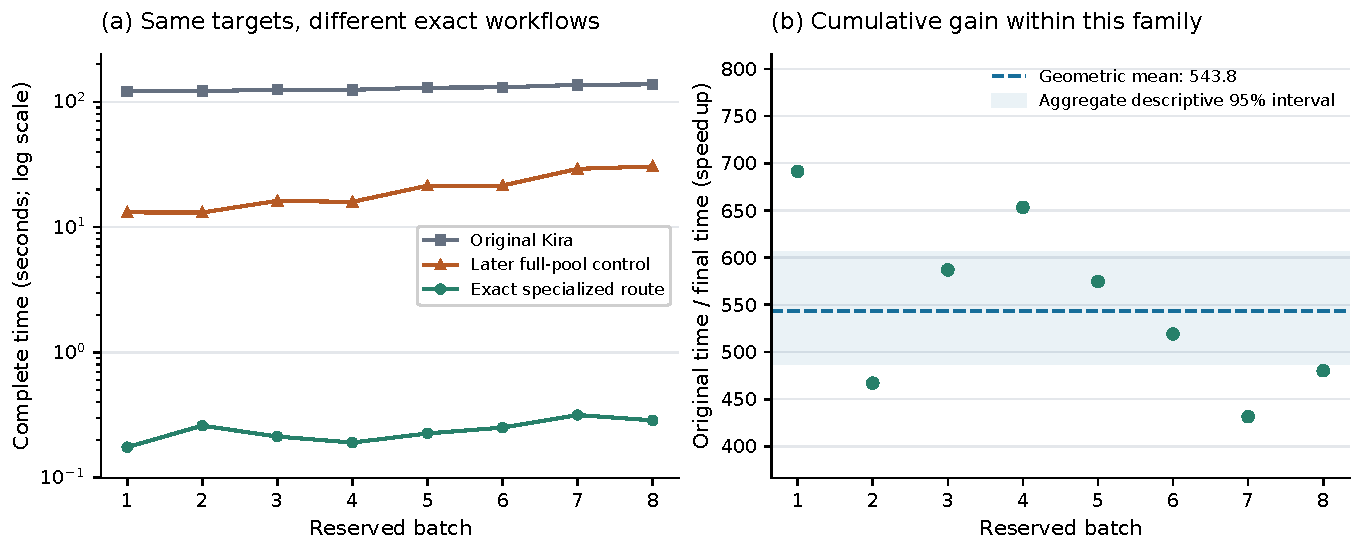
\includegraphics[width=\linewidth]{paper_figures/cumulative_results.pdf}
\caption{Exact recurrence reuse gives the large saving in the restricted vacuum family. Left: complete times on a logarithmic axis. Right: original time divided by final time. Each batch contains three mass profiles at loops 1--12. The result combines mathematical reuse and program improvements.}
\label{history:fig:cumulative}
\end{figure}

This result depends on the structure of the family. The benchmark constructs Euler and mass partial-fraction identities rather than a general high-loop IBP system. Earlier checks at loop orders 13, 16, 24, and 32 use the same family, and the recurrence proof applies to every positive integer loop order under its stated assumptions. The demonstrated high-loop result therefore concerns this restricted vacuum problem; the connected scattering comparisons in Sections~\ref{sec:components} and~\ref{sec:adaptive} have separate definitions and timings.

\subsection{Training data and experimental design}
\label{history:sec:data}
\subsubsection{Constructing targets with known reductions}
To train the original models, we need targets together with master coefficients and a recorded sequence of valid reduction steps. We obtain these data by working backwards from checked master relations. If $E_q=\sum_i A_{qi}I_i=0$ is a source identity, we construct
\begin{equation}
 T=\sum_m r_mM_m+\sum_q\lambda_qE_q,
 \qquad \lambda_q,r_m\in\Q(\boldsymbol x,d).
 \label{history:eq:reverse}
\end{equation}
Expanding the right-hand side produces an expression in indexed integrals while the added zero identities leave its master coefficients unchanged. We record the identities, their seeds and operators, and the operations used in the construction. Appendix~\ref{history:app:construction} proves the relation and explains how to recover a reduction path from this record.

This procedure usually produces a sum of integrals. It produces a single indexed integral only when the expanded expression has that form. It also supplies one sufficient seed set and one valid reduction path; it does not establish that either has minimum cost. The labels therefore teach the original models to reproduce a checked construction, and later timing experiments determine whether their choices help Kira.

\subsubsection{Coverage and separation of training and test data}
Table~\ref{history:tab:data} summarizes the original collection. The 17,100 family instances contain 57,979 master entries, counted separately in each family, and 2,301,272 targets. Many instances are parameter variations of the same graph. We call a specified assignment of masses and momentum invariants a \emph{parameter profile}. In particular, the higher-loop additions use the restricted vacuum family derived in Appendix~\ref{history:app:vacuum}; they do not represent general scattering graphs through twelve loops. The test set contains 148,494 single integrals and 541,888 integral expressions. Appendices~\ref{history:app:families} and \ref{history:app:basis} specify the families and the checks used to establish their master bases.

\begin{table}[!htbp]
\centering\small
\caption{Original constructed data. Family instances include parameter variations of the same graph.}
\label{history:tab:data}
\begin{tabular}{@{}lrr@{}}\toprule
Part & Family instances & Targets\\\midrule
Training & 11,963 & 1,610,890\\
Testing & 5,137 & 690,382\\
Total & 17,100 & 2,301,272\\\bottomrule
\end{tabular}
\end{table}

Related mass assignments remain in the same training or test group at every loop order. The seed and row networks each receive twenty additional passes through the expanded training set, starting from their earlier parameters and optimizer state. Some test profiles had already appeared in earlier evaluations, so these results concern reserved parameter groups rather than entirely new graph structures. The later native-Kira studies use separate training, validation, and test samples: training fits the models, validation selects their settings, and the reserved test measures those fixed choices.

\subsubsection{What the timing comparisons measure}
Within each comparison, every method receives the same targets and prescribed master basis and uses the same allocated resources. We use \emph{complete reduction time} for the measured time that includes input preparation, model prediction, algebra, checks, and all fallback attempts. Offline training and the construction of reference answers are excluded. The original local-model comparisons repeat each calculation five times. The final complete-cost comparisons use three repetitions, with the method order rotated. Each comparison reports batch medians and states its repetition count.

The baseline also needs to be specified. Most native comparisons use the same modified Kira 3.1 executable for learned and native choices, so improvements shared by that executable do not count as a benefit of the model. The cumulative vacuum comparison instead uses the saved original executable as its baseline. Later sections also distinguish the sum of batch median times from a geometric mean that gives each graph equal weight. The latter averages logarithms of time ratios and then exponentiates the result. Appendix~\ref{history:app:timing} defines these measures and their descriptive uncertainty intervals. Keeping these conditions explicit allows each speedup to be interpreted against the calculation it actually measures.

\subsection{Learning the three reduction decisions}
\label{history:sec:local-models}
We first test the three decisions separately. For each model, we describe the information it receives, the reference labels used in training, and its effect on exact reduction time. This separates the ability to reproduce a recorded choice from the ability to accelerate Kira.

\subsubsection{Model 1: selecting seeds}
\label{history:sec:seeds}
The seed network receives the terms of the target, its family, the master indices, and a finite list of candidate seeds. It maps each target term to 32 learned numerical features and combines these with ordered pairs of terms and information about the family and masters. A seed-dependent attention operation then identifies which target terms are most relevant to that candidate. The shared representations and attention follow Refs.~\cite{DeepSets,AttentionIsAllYouNeed}; Appendix~\ref{history:app:models} gives the full architecture.

The network has 28,097 fitted parameters and assigns a separate score to every candidate:
\begin{equation}
 p_b=\frac{1}{1+e^{-g_\theta(T,F,\mathcal M,\boldsymbol\sigma_b)}},
 \qquad
 \widehat\Sset(T)=\{\boldsymbol\sigma_b\in\Cset:p_b\geq\tfrac12\}.
 \label{history:eq:seed}
\end{equation}
Here $F$ denotes the family, $\mathcal M$ the master list, $\Cset$ the candidate list, and $g_\theta$ the output of the network with fitted parameters $\theta$. The score estimates whether a seed belongs to the recorded sufficient set. Because a target can require several seeds, several scores can exceed the selection threshold and their sum need not be one. Training uses binary cross-entropy and AdamW~\cite{AdamW}. The network receives neither the target's final master coefficients nor its later reduction steps.

On the 690,382 reserved targets, the model has precision 95.750\%, recall 96.892\%, and $F_1$ score 96.318\%. Its complete predicted set matches the recorded set for 84.332\% of targets. Kira reduces 652,517 targets with the predicted sets, corresponding to 94.515\% sufficiency, and reduces all targets when the full equation pool is available. These percentages differ because matching the recorded set and supplying enough equations are different tests: another seed set can also be sufficient. Appendix~\ref{history:app:timing} defines the metrics. We report precision and recall because the large number of negative labels can make overall classification accuracy misleading~\cite{SaitoRehmsmeier2015}.

To determine whether this prediction saves time, we use a separate comparison on existing identity pools from twelve reserved one-loop box instances. The weights remain fixed, and the timing test uses threshold $0.01$, chosen before that comparison; the earlier label and sufficiency tests use $1/2$. Both the learned selector and a distance-based rule receive the same basis check and full-pool fallback. For single targets, the learned-to-full-pool time ratio is $0.914$, with descriptive 95\% interval $[0.871,0.958]$, giving 8.6\% less time. Relative to the distance rule, the ratio is $0.913$ with interval $[0.855,0.972]$, giving 8.7\% less time. Every method completes all five repetitions of these twelve cases.

The gain is less clear for larger requests. For sixteen-target batches, the ratio is $0.952$ with interval $[0.772,1.148]$, which includes equal time. Across the full planned seed comparison, 345 trials finish exactly, three remain incomplete, and twelve repetitions are skipped; the timing summary uses only complete paired cases. The identity pools already exist when these timers start. A separate native test that includes IBP generation gives ratio $1.096$ with interval $[0.963,1.275]$. Thus the original network demonstrates a saving for the stated supplied-equation single-target test, while native generation requires a different assessment. Section~\ref{history:sec:adaptation} reports new seed trees trained directly on scattering reductions.

\begin{figure}[tbp]
\centering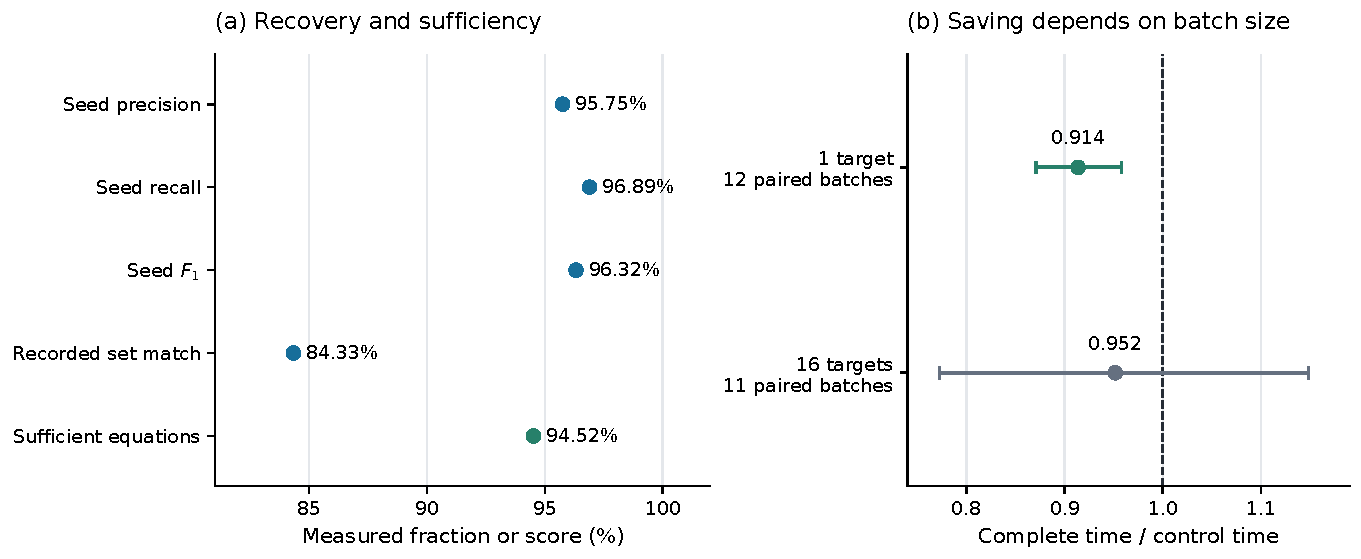
\includegraphics[width=\linewidth]{paper_figures/seed_results.pdf}
\caption{Seed prediction accuracy and reduction speed measure different outcomes. Left: results on the original reserved targets. Right: learned time divided by full-pool time. Values below one are faster. The single-target interval lies below one; the sixteen-target interval crosses it.}
\label{history:fig:seed}
\end{figure}

\FloatBarrier

\subsubsection{Model 2: selecting elimination rows}
\label{history:sec:rows}
After the equations have been generated, several allowed source rows may eliminate the next integral. The row network scores these alternatives using 132 inputs that describe the pivot integral, nonzero entries, family, matrix size, and sampled cancellations. It maps each action to 32 learned features, combines information across the available actions, and passes the result through a hidden layer with 64 components. A softmax converts the final scores into probabilities that sum to one, and the network selects the action with the largest probability. The 10,529 fitted parameters determine the choice; exact arithmetic performs the row operation. Appendices~\ref{history:app:ibp} and \ref{history:app:models} give the operation and architecture.

The original training examples follow one changing target row while the source identities stay fixed. On 2,558,472 reserved states with a choice, the network selects the recorded action in 95.845\% of cases, compared with 99.473\% for a local deterministic rule. Complete predicted paths agree with the saved master row at three finite-field points for 690,302 of 690,382 targets. These sampled checks support agreement at those points but do not prove symbolic equality. Including prediction, the network takes 17.657 times as long as the local rule.

The more relevant application places the fixed network inside Kira's changing symbolic matrix and preserves Kira's allowed integral order. Across 84 exactly checked trials, this implementation takes 1.305 times the time of stock Kira. We therefore also test smaller policies trained on measured algebraic cost, with compiled prediction and shared features. The latest row-only comparison gives ratio $0.982$ with interval $[0.959,1.003]$, while combining it with the seed policy gives $1.100$ with interval $[0.966,1.279]$ against native choices.

Figure~\ref{history:fig:row} shows that the later intervals still include equal time. We therefore retain Kira's row choices in the final method. This result explains why the remaining studies focus on decisions that can avoid equation generation or repeated work: reproducing a plausible elimination path did not, by itself, provide a reliable reduction in complete time.

\begin{figure}[tbp]
\centering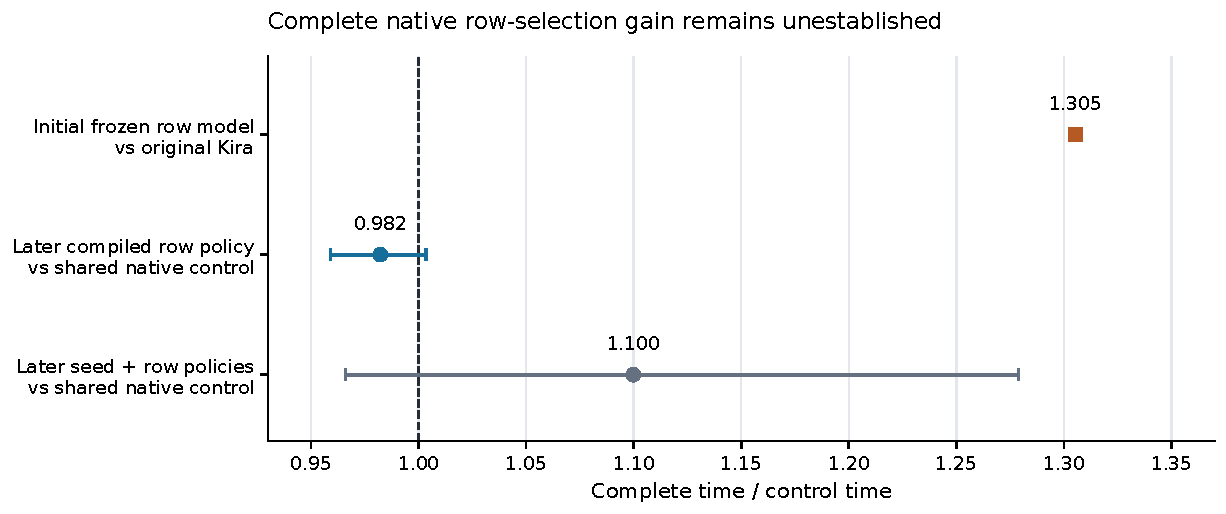
\includegraphics[width=0.96\linewidth]{paper_figures/row_results.pdf}
\caption{The row model gives no reliable complete-time saving. The first model is slower, and the later row-only interval includes equal time. The original summary provides no interval for the first result. These comparisons use different model versions.}
\label{history:fig:row}
\end{figure}

\FloatBarrier

\subsubsection{Model 3: selecting individual equations}
\label{history:sec:equations}
Equation selection offers an earlier opportunity to avoid work. The model scores each seed--operator pair before Kira constructs its symbolic coefficients. Its seventeen inputs describe the family, target list, seed indices, and operator; they include the number of loops and targets, extra propagator powers, numerator rank, and distance between seed and target indices. A classification tree~\cite{CART1984} applies feature-threshold decisions and returns a score from its final leaf. The score estimates whether the equation belongs to the useful part of a recorded native reduction. No equation coefficients are needed for prediction, and Kira retains its native treatment of symmetries and masters.

The original fit uses 153,124 candidate equations, including 12,270 positive labels, from fourteen batches in eight parameter profiles. The four graph structures are the two-loop sunrise, planar double box, three-loop vacuum, and three-loop ladder. Validation compares trees of depth eight and twelve, containing 295 and 1,335 nodes, at threshold $0.01$. It selects the deeper tree for the double box and the shallower tree for the vacuum and ladder; the 21-target sunrise case retains the preceding equation policy. A filter is enabled only when validation shows lower complete and preparation times without fallback. Adding learned seed or row choices fails this condition, so native seed and row choices remain active in this comparison.

Testing uses eight new parameter profiles and fourteen target batches. The masses and momentum invariants take rational values, while $d$ remains symbolic, so the coefficient field is $\Q(d)$. Five repetitions of four methods give 280 complete calculations. Native choices, the early equation model, and the distance-based control share the same executable improvements; a fourth method uses the preceding release. This design distinguishes the effect of equation selection from improvements in the surrounding implementation.

Relative to native choices in that executable, the model reduces complete time by 5.7\% and equation-preparation time by 36.2\%. The corresponding ratios are $0.943$ with interval $[0.915,0.970]$ and $0.638$ with interval $[0.546,0.734]$. Preparation includes modular generation, selection, modular solving, and symbolic equation regeneration. The smaller change in complete time reflects the work that remains after preparation. All 280 calculations succeed on their first attempt, and independent exact checks cover 94,970 coefficient comparisons and eight applications supplied only with the prescribed basis.

\begin{figure}[tbp]
\centering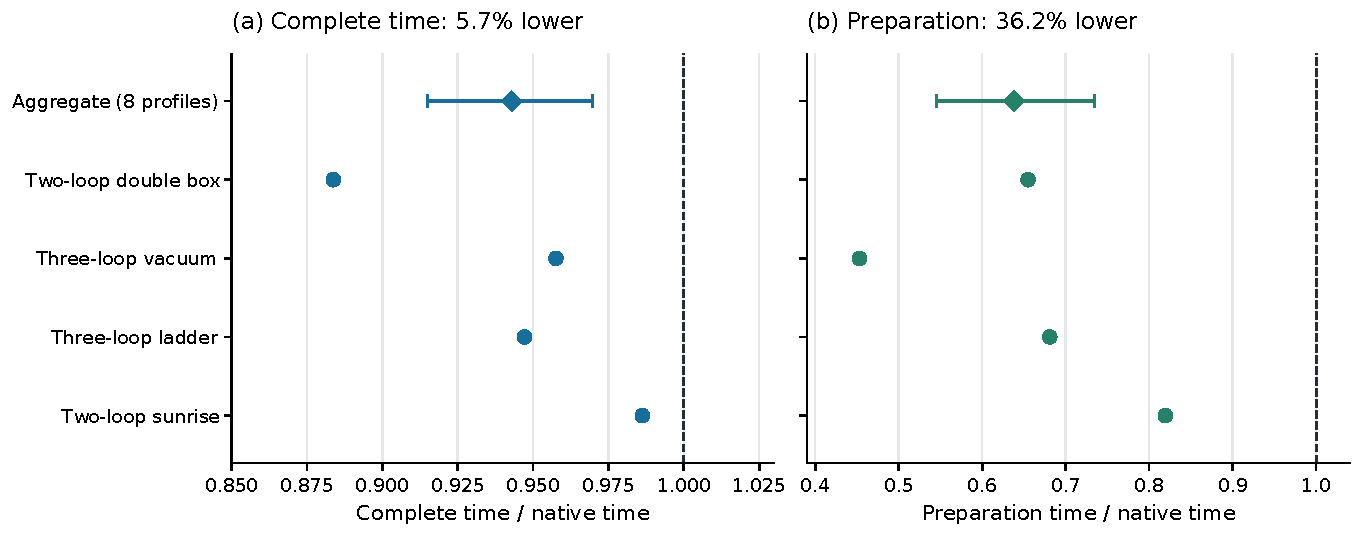
\includegraphics[width=\linewidth]{paper_figures/equation_results.pdf}
\caption{Equation selection saves more preparation time than complete reduction time. Each ratio compares the model with native choices in the same executable. The panels use different labelled ranges. The aggregate intervals describe variation across the eight profiles.}
\label{history:fig:equations}
\end{figure}

To test how far the original tree transfers, we also apply the fixed depth-twelve model to three structures absent from its training data: a massless nonplanar two-loop box, a massless pentagon, and a box with one external virtuality. Appendix~\ref{history:app:families} defines their propagators and invariants, using the massless limit of the nonplanar family in Ref.~\cite{KiraOriginal}. Four batches use rational kinematics and symbolic $d$. Three more keep the independent invariants symbolic, with coefficient fields $\Q(d,s,t)$, $\Q(d,s_{12},s_{23},s_{34},s_{45},s_{51})$, and $\Q(d,s,t,v)$. Here $s,t$ are four-point invariants, $s_{i,i+1}$ are adjacent five-point invariants, and $v$ is an external squared momentum.

The seven batches contain 88 targets and produce seventy comparison calculations. All final results pass exact checks, but every one of the 35 filtered calculations needs native fallback. The average time ratio is $1.252$, or 25.2\% more time. Checks cover 5,600 coefficient pairs, agreement with enlarged seed regions in all seven cases, and agreement after new rational substitutions in the three symbolic cases. The fallback therefore restores a correct answer at an additional cost. Figure~\ref{history:fig:transfer} records this transfer test before the new training described next.

\begin{figure}[tbp]
\centering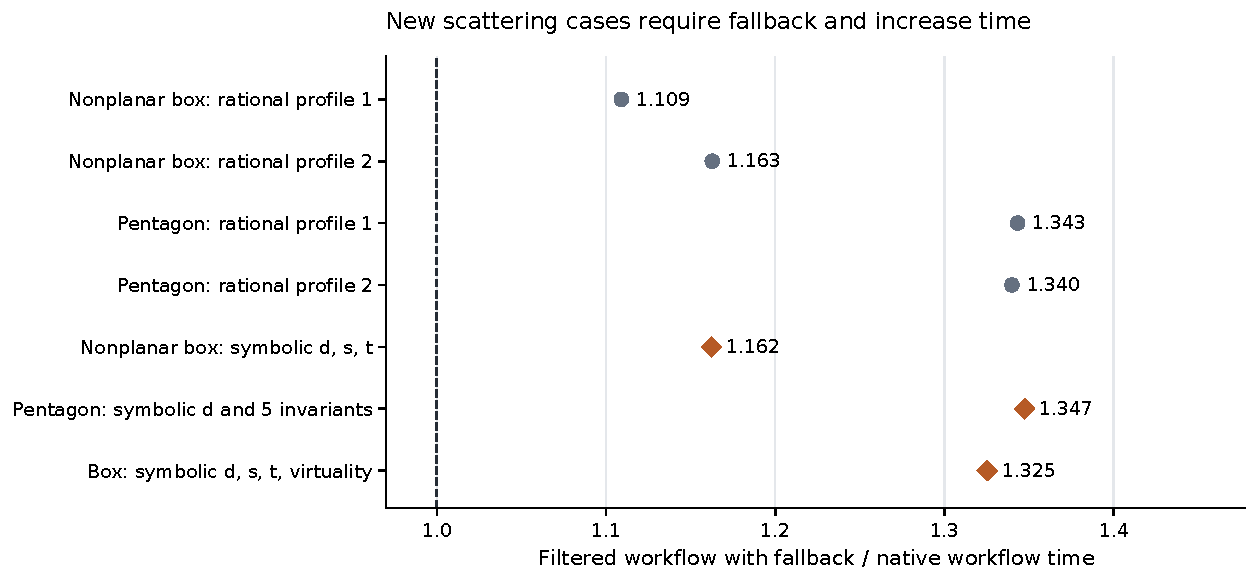
\includegraphics[width=\linewidth]{paper_figures/transfer_results.pdf}
\caption{The original equation model is slower on the new scattering structures. Each point compares five-run median times, including fallback. All 35 filtered calculations require a retry. This historical test uses the original weights, before additional training.}
\label{history:fig:transfer}
\end{figure}

\FloatBarrier
\providecommand{\StudySection}{\section}
\providecommand{\StudySubsection}{\subsection}

\StudySection{Training on the additional scattering structures}
\label{history:sec:adaptation}
The transfer failures raise a specific question: can examples from the missing structures teach a filter to retain enough equations? To test this, we train a new seed tree and equation tree for each of the nonplanar box, pentagon, and box with external virtuality. The original models remain fixed for comparison. Appendix~\ref{history:app:models} defines the new reference labels and tree fits.

Table~\ref{history:tab:scattering-split} separates the training, validation, and test batches. Rational batches use different invariant values in each split, while symbolic batches keep the independent invariants symbolic and use disjoint target lists. The graph structures occur in all three splits. Thus the test measures learning within these structures and separates that question from transfer to an unseen graph.

\begin{table}[!htbp]
\centering\small
\caption{The additional scattering study. Each of the three structures contributes equally to the batch counts.}
\label{history:tab:scattering-split}
\begin{tabular}{@{}lrrr@{}}\toprule
Part & Rational batches & Symbolic batches & Targets\\\midrule
Training & 6 & 3 & 108\\
Validation & 3 & 3 & 60\\
Testing & 6 & 3 & 108\\\bottomrule
\end{tabular}
\end{table}

Each tree has maximum depth twelve. The seed tree uses sixteen features and gives all operators of a seed the same score; the equation tree also receives the operator index, giving seventeen features and allowing different decisions for different operators. In both cases Kira enumerates its usual seed region, the tree filters candidates before coefficient construction, and native elimination remains active. These fits produce new trees trained on native reductions, while the original neural networks remain unchanged.

The fits use 59,706 equation records and 4,674 grouped seed records, including candidate patterns repeated in different training batches. Table~\ref{history:tab:scattering-fit} gives the tree sizes. Validation compares three score thresholds and fixes a setting before the reserved test. The four test methods are native choices, the original equation tree, the new seed tree, and the new equation tree. Five repetitions on identical targets give 180 calculations, with prediction, exact algebra, coefficient checks, cleanup, and fallback included in the timer. Reference discovery, training, and later recording of results are excluded.

\begin{table}[!htbp]
\centering\small
\caption{Additional training records and tree sizes. Each graph uses three training batches.}
\label{history:tab:scattering-fit}
\begin{tabular}{@{}lrrrr@{}}\toprule
Structure & Seed records & Seed nodes & Equation records & Equation nodes\\\midrule
Nonplanar box & 4,326 & 67 & 56,238 & 819 \\
Pentagon & 258 & 15 & 2,838 & 179 \\
Box with virtuality & 90 & 11 & 630 & 81 \\
\bottomrule
\end{tabular}
\end{table}

All 180 calculations pass exact checks of 9,880 returned coefficient entries. Eighteen additional applications receive the target and prescribed basis without reference coefficients, and their answers also pass an independent comparison after reduction. Each new selector completes all 45 timed attempts without fallback, whereas the original equation model needs fallback in all 45 trials. The new training therefore improves sufficiency on these inputs.

The timing result is more limited. Relative to native choices, the new seed model has ratio $1.027$ with descriptive 95\% interval $[0.995,1.086]$, and the new equation model has ratio $1.017$ with interval $[0.988,1.054]$. Their measured average times are 2.7\% and 1.7\% higher, respectively. The original filter has ratio $1.368$, or 36.8\% more time, on this new test. Its earlier 25.2\% overhead refers to different parameter points and symbolic targets. The additional training removes much of the fallback cost but does not establish an overall saving against native Kira.

\begin{table}[!htbp]
\centering\small
\caption{New reserved test results. Each value uses five repetitions. Ratios divide model time by native time; values below one are faster.}
\label{history:tab:scattering-time}
\begin{tabular}{@{}lrrrr@{}}\toprule
Case & Native (s) & Original tree & New seeds & New equations\\\midrule
Nonplanar box (13) & 4.163 & 1.293 & 1.023 & 0.980 \\
Nonplanar box (14) & 4.140 & 1.221 & 1.002 & 0.974 \\
Nonplanar box (symbolic) & 4.458 & 1.233 & 0.983 & 1.010 \\
Pentagon (13) & 1.005 & 1.439 & 0.963 & 1.016 \\
Pentagon (14) & 0.965 & 1.436 & 1.069 & 1.038 \\
Pentagon (symbolic) & 1.120 & 1.356 & 0.958 & 0.979 \\
Box with virtuality (13) & 0.826 & 1.339 & 0.953 & 0.991 \\
Box with virtuality (14) & 0.763 & 1.529 & 1.152 & 1.124 \\
Box with virtuality (symbolic) & 0.729 & 1.499 & 1.166 & 1.052 \\
\midrule
Geometric mean ratio & --- & 1.368 & 1.027 & 1.017\\\bottomrule
\end{tabular}
\end{table}

The individual results in Table~\ref{history:tab:scattering-time} and Figures~\ref{history:fig:adapted-time}--\ref{history:fig:adapted-sufficiency} explain this distinction. Some new filters reduce time, while others add overhead to cases that native Kira already solves quickly. We therefore retain native choices as the default for this scattering study. The result supports training on the missing structures to improve sufficiency, although it cannot isolate missing data as the sole cause of the original failure: the study also changes the seed-model architecture and fits separate trees for each graph. The intervals resample the three graph groups and describe this limited comparison.

\begin{figure}[tbp]
\centering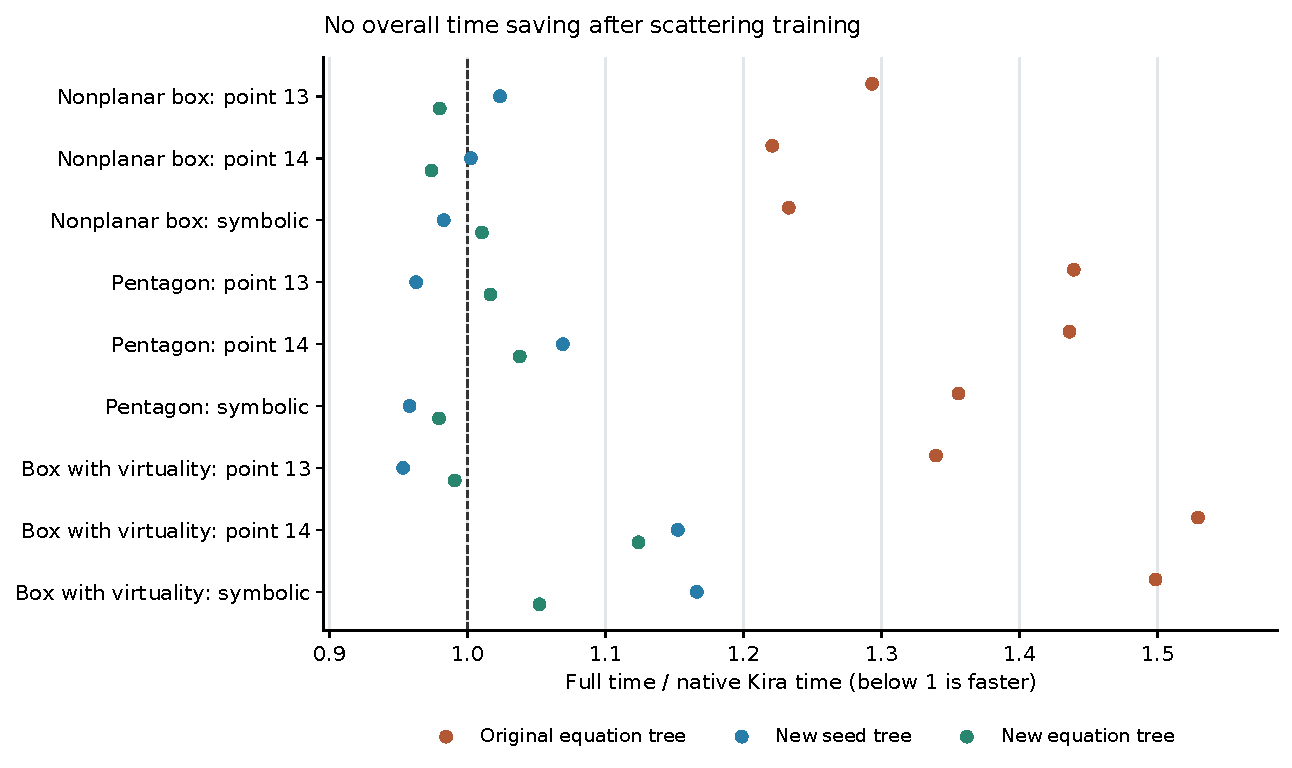
\includegraphics[width=\linewidth]{paper_figures/scattering_training.pdf}
\caption{Training on the three structures removes much of the original filter's overhead, but gives no overall saving against native Kira. Points compare five-run median complete times, including prediction, checks and fallback. The dashed line marks equal time. No per-case uncertainty interval is inferred from five repetitions.}
\label{history:fig:adapted-time}
\end{figure}

\begin{figure}[tbp]
\centering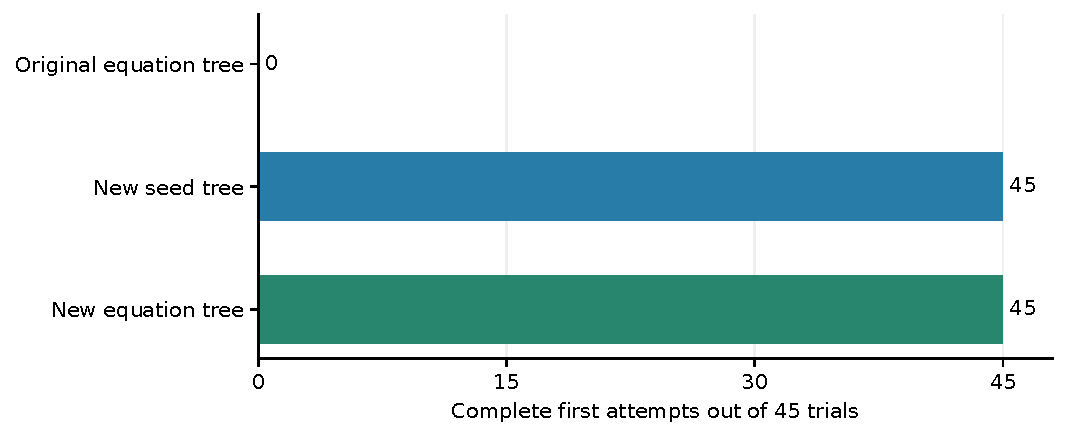
\includegraphics[width=.85\linewidth]{paper_figures/scattering_sufficiency.pdf}
\caption{The new selectors provide sufficient equations on every first attempt. Each method has 45 trials across nine batches. Native fallback lets the original filter eventually complete, and its added time remains in the comparison above.}
\label{history:fig:adapted-sufficiency}
\end{figure}

\FloatBarrier


\subsection{IBP relations and exact elimination}
\label{history:app:ibp}
This appendix derives the identities and row operations used throughout the study. For a seed $\boldsymbol\sigma$, write its denominator product as $P_{\boldsymbol\sigma}=\prod_iD_i^{-\sigma_i}$ and define $\partial_k^\mu=\partial/\partial\ell_{k\mu}$. The product rule separates the derivative in Eq.~\eqref{history:eq:ibp} into a derivative of the momentum vector and a derivative of the propagator factors:
\begin{align}
 \partial_k^\mu(v_\mu P_{\boldsymbol\sigma})
 &= (\partial_k\cdot v)P_{\boldsymbol\sigma}
       +v\cdot\partial_k P_{\boldsymbol\sigma},\\
 v\cdot\partial_k P_{\boldsymbol\sigma}
 &=-\sum_i\sigma_i(v\cdot\partial_kD_i)
       D_i^{-\sigma_i-1}\prod_{j\ne i}D_j^{-\sigma_j}.
 \label{history:eq:ibp-expanded}
\end{align}
When $v=\ell_h$, the first derivative is $\partial_k\cdot v=d\delta_{kh}$, where $\delta_{kh}$ equals one for $k=h$ and zero otherwise; for an external momentum it vanishes. The integrated total derivative is zero in a region of convergence, and analytic continuation extends the relation to dimensional regularization~\cite{ChetyrkinTkachov,Weinzierl2022}. The same regularization prescription sets scaleless integrals to zero.

With a complete scalar-product basis, the scalar numerator $v\cdot\partial_kD_i$ can be written as $u_i+\sum_j v_{ij}D_j$. The coefficients $u_i$ and $v_{ij}$ depend on masses, invariants and the chosen momentum routing. Substituting in Eq.~\eqref{history:eq:ibp-expanded} gives
\begin{equation}
 0=\delta_v I_{\boldsymbol\sigma}
 -\sum_i\sigma_i u_i I_{\boldsymbol\sigma+\boldsymbol e_i}
 -\sum_{i,j}\sigma_i v_{ij}
       I_{\boldsymbol\sigma+\boldsymbol e_i-\boldsymbol e_j},
 \label{history:eq:ibp-shifts}
\end{equation}
Here $\delta_v=\partial_k\cdot v$, and the unit vector $\boldsymbol e_i$ increases index $i$ by one. The derivative therefore relates the seed integral to integrals with shifted integer indices. Auxiliary denominators complete an otherwise incomplete scalar-product representation. When the denominator representation is dependent, additional algebraic relations are needed; the restricted vacuum family in Appendix~\ref{history:app:vacuum} uses explicit mass partial fractions.

Suppose row $q$ of such a system satisfies $\sum_jA_{qj}I_j=0$ and $A_{qk}\ne0$. Solving this row for the pivot integral gives
\begin{equation}
 I_k=-\sum_{j\ne k}\frac{A_{qj}}{A_{qk}}I_j.
 \label{history:eq:pivot}
\end{equation}
For a second identity row, or a target coefficient row $r$, subtract $(A_{rk}/A_{qk})$ times the zero identity. The resulting coefficients are
\begin{equation}
 A'_{rj}=A_{rj}-\frac{A_{rk}}{A_{qk}}A_{qj},
 \qquad A'_{rk}=0.
 \label{history:eq:row}
\end{equation}
Because the subtracted identity is zero, this operation preserves the target while removing its pivot entry. Choosing a different allowed source row can change the intermediate expressions and their cost without changing that equality. Repeated elimination removes the nonmaster columns and yields Eq.~\eqref{history:eq:master}, provided each pivot coefficient is nonzero. Kinematic points at which a required denominator vanishes require a separate calculation.

\subsection{Reverse construction and the meaning of reference labels}
\label{history:app:construction}
The reverse construction provides targets with known answers because each checked source identity $E_q$ is a linear combination of integrals that equals zero. Substituting these identities into Eq.~\eqref{history:eq:reverse} gives
\begin{equation}
 T-\sum_mr_mM_m=\sum_q\lambda_qE_q=0.
 \label{history:eq:reverse-check}
\end{equation}
The equality fixes the master coefficients of the constructed expression. Expanding the source identities and collecting terms with equal index vectors then gives the target supplied to the model. Recording the operations, source rows, and seed--operator labels provides a path back to the masters. The coefficients $\lambda_q$ and $r_m$ may be rational functions, including constants as a special case. Algebraic mass partial-fraction identities are recorded separately because they have no IBP seed label.

Different zero identities can give different construction histories for the same target. A saved seed set is therefore sufficient, but need not be unique or smallest. Likewise, the saved row sequence need not use the fewest operations. A seed label records membership in one checked set, and a row label records the next step in one checked path. The final master coefficients and later steps do not enter the model inputs.

\subsection{Model specification and training objectives}
\label{history:app:models}
This appendix specifies what each model learns and how its training objective is obtained. We begin with the seed network, whose symbolic target coefficients must first be represented by numerical inputs. We split each expression into tokens and count individual tokens and consecutive pairs and triples. A fixed signed map places these counts in 64 components. Different token groups can share a component, so equal representations do not prove equal expressions. Integral indices, complexity counts and term positions give further inputs. A shared hyperbolic-tangent map converts each term into a vector $\boldsymbol h_u\in\mathbb R^{32}$. Family symbols, master indices and candidate indices give separate 32-component vectors.

\subsubsection{Seed representation and loss}
The target representation includes the following summary of ordered term pairs:
\begin{equation}
 \boldsymbol h_{\rm pair}=
 \frac{1}{n_T(n_T-1)}\sum_{u\ne v}
 \psi_\theta([\boldsymbol h_u,\boldsymbol h_v,
       \boldsymbol h_u-\boldsymbol h_v,
       \boldsymbol h_u\odot\boldsymbol h_v]),
 \label{history:eq:pair}
\end{equation}
where $n_T$ is the number of terms, square brackets concatenate vectors, $\odot$ multiplies components and $\psi_\theta$ returns 32 components. For $n_T=1$, the summary is zero. This definition covers ordered pairs, not all larger term subsets. The candidate vector $\boldsymbol u_b$ weights target terms through scaled dot-product attention~\cite{AttentionIsAllYouNeed}:
\begin{equation}
 w_{bu}=\frac{\exp(\boldsymbol u_b\cdot\boldsymbol h_u/\sqrt{32})}
 {\sum_v\exp(\boldsymbol u_b\cdot\boldsymbol h_v/\sqrt{32})},
 \qquad \boldsymbol v_b=\sum_u w_{bu}\boldsymbol h_u.
\end{equation}
The final input combines the mean and componentwise maximum of the term vectors with the pair, family, basis, seed, and attention-weighted term vectors. A hidden layer with 64 components produces $g_\theta$ in Eq.~\eqref{history:eq:seed}. Shared maps and aggregation follow Ref.~\cite{DeepSets}, while stored positions retain the target term order. Reordering the candidate seeds changes only the order of the output scores.

If $y_b\in\{0,1\}$ is recorded seed membership, a Bernoulli model assigns label likelihood $p_b^{y_b}(1-p_b)^{1-y_b}$. Taking its negative logarithm gives $-y_b\log p_b-(1-y_b)\log(1-p_b)$. Averaging within each candidate list and then across targets gives the implemented loss
\begin{equation}
 \mathcal L_s=-\frac{1}{|\mathcal D_s|}\sum_{T\in\mathcal D_s}
 \frac{1}{|\Cset(T)|}\sum_{b\in\Cset(T)}
 [y_b\log p_b+(1-y_b)\log(1-p_b)].
 \label{history:eq:seed-loss}
\end{equation}
Here $\mathcal D_s$ is the training-target set. This objective treats each target equally and does not claim that true seed dependencies are statistically independent. Training uses AdamW~\cite{AdamW} with learning rate $10^{-3}$, weight decay $10^{-4}$, gradient norm limit one and up to 32 targets per update. The threshold $1/2$ stays fixed during the expanded label test.

\subsubsection{Row representation and loss}
The row network compares the actions available at the current matrix state. Let $\mathcal A$ be that action list, and let $\boldsymbol f_a\in\mathbb R^{132}$ be the feature vector for action $a$. The encoder is $\boldsymbol h_a=\tanh(W\boldsymbol f_a+\boldsymbol b)$ with 32 components. Concatenating $\boldsymbol h_a$ with the mean and componentwise maximum over $\mathcal A$ gives the input to a 64-component hidden layer. Its scalar output $g_a$ defines
\begin{equation}
 p(a\mid A,\mathcal A)=\frac{e^{g_a}}{\sum_{b\in\mathcal A}e^{g_b}},
 \qquad
 \mathcal L_r=-\frac{1}{|\mathcal D_r|}
       \sum_{(A,\mathcal A,a^*)\in\mathcal D_r}\log p(a^*\mid A,\mathcal A).
 \label{history:eq:row-loss}
\end{equation}
Here $A$ is the matrix, $a^*$ is the recorded action, and $\mathcal D_r$ contains the training states with a choice. The softmax denominator normalizes the probabilities to one, and taking the negative logarithm of the recorded action's probability gives the loss. A state with one action has zero loss. Training uses the seed model's AdamW settings and 256 states per update. Trial updates modulo a prime provide cancellation features. The numerical size of a modular value does not measure the size of a real coefficient.

Later row models learn the cost of an action. One fit predicts the logarithm of the measured insertion time. Another counts the remaining forward insertions after that action, with Kira choosing later steps. If insertion $j$ uses $n_j$ source entries, its estimated cost is $1+2n_j$: one division, followed by a multiplication and subtraction for each entry. Thus the cost label is $C(S,q)=\sum_j(1+2n_j)$ for state $S$ and choice $q$. The later tree fits
\begin{equation}
 y_q=\frac{C(S,q)-C(S,0)}{\max\{1,\max_b C(S,b)-\min_b C(S,b)\}},
 \qquad \widehat y_q=h(\boldsymbol x_q-\boldsymbol x_0),
\end{equation}
where $0$ denotes Kira's native source and $\boldsymbol x_q$ contains eighteen current-row and overlap features. Weighted squared error gives each training family equal weight. Validation selects the tree and the required predicted improvement, and exact coefficients must agree before a measured continuation enters training. This count describes coefficient operations, while complete timings include the algebraic work inside each coefficient operation. Neither training objective proves a globally minimum path.

\subsubsection{Equation features and tree fitting}
The equation model uses a reference label derived from the support of an equation, meaning the set of integrals with nonzero coefficients. An equation label records whether this support appears in Kira's selected system. Table~\ref{history:tab:features} groups the equation tree's seventeen inputs. They describe the seed and target before symbolic coefficient construction. For seed indices $\boldsymbol\sigma$ and target indices $\boldsymbol a$, the distance is $\sum_i|\sigma_i-a_i|$. The additional-power count is $\sum_i\max(\sigma_i-1,0)$, and the numerator rank is $\sum_i\max(-\sigma_i,0)$. Neither quantity requires equation coefficients.

\begin{table}[!htbp]
\centering\small
\caption{Inputs to the original equation tree. The scattering seed trees omit the operator input and use sixteen features.}
\label{history:tab:features}
\begin{tabularx}{\linewidth}{@{}lYr@{}}\toprule
Group & Quantities & Number\\\midrule
Family and request & Loops, external momenta, index count, logarithm of target count & 4\\
Seed & Positive indices, additional powers, numerator rank & 3\\
Target limits & Excess seed powers and rank above target maxima & 2\\
Sector & Whether requested; excess powers and rank above its target maxima & 3\\
Target distance & Minimum index distance; whether the seed is a target & 2\\
Operator & IBP operator index & 1\\
Overall limits & Maximum target powers and numerator rank & 2\\\bottomrule
\end{tabularx}
\end{table}

Training gives each physical profile equal total weight by assigning each row weight $1/(n_b B_g)$, where $n_b$ is its batch size and $B_g$ is the number of training batches in its profile. At a node, let $w_+,w_-$ be the positive and negative total weights. Half the weighted binary Gini impurity is
\begin{equation}
 H=\frac{w_+w_-}{w_++w_-}.
\end{equation}
Indeed, with $p=w_+/(w_++w_-)$, the weighted Gini expression is $(w_++w_-)[1-p^2-(1-p)^2]=2H$. Each proposed split reduces $H$ by the sum of its two children's values. The fit tests 25 feature quantiles between 0.02 and 0.98, rejects children below the stated population limit, and selects the largest positive reduction. This is the classification-tree construction of Ref.~\cite{CART1984} with our bounded set of candidate splits.

A leaf with $n_+$ positive rows among $n$ rows returns
\begin{equation}
 p_{\rm leaf}=\frac{n_++1/2}{n+1}.
\end{equation}
Adding one half-count to each class gives a finite score even when a leaf contains only one class. The original tree keeps an equation when $p_{\rm leaf}\geq0.01$. These scores estimate reference-set membership; they are not calibrated probabilities that the whole reduction succeeds. The depth-eight and depth-twelve fits require at least 24 and eight rows in each child. The split procedure follows Ref.~\cite{CART1984}. A basis check and fallback still test whether the selected system is sufficient.

\subsubsection{Additional scattering seed and equation trees}
The added scattering study fits a separate pair of trees for each of the three graph structures. The equation labels use the same selected-support rule as the original equation model. Let $y_{\sigma,o}$ be one when the native selected system contains the recorded equation support for seed $\sigma$ and operator $o$. A seed receives label one when any of its operators has label one:
\begin{equation}
 y_\sigma=\max_o y_{\sigma,o}.
 \label{history:eq:adapted-seed-label}
\end{equation}
For binary labels, this maximum is one exactly when at least one selected-support equation comes from the seed. This proves the stated membership rule. The label gives a useful reference set, not a proof that every labelled seed is necessary.

Each seed appears once per training batch. Its tree uses the sixteen features that do not depend on the operator. Thus every operator of that seed receives the same score. The early filter either permits or skips construction of all its equations. Kira still enumerates the seed region and applies its native symmetries. The equation tree uses all seventeen features and can keep different operators of the same seed.

Both fits have maximum depth twelve and at least eight records in each child. Each training batch has equal total weight. The split rule and leaf score are those derived above. Validation compares thresholds $0.001$, $0.01$ and $0.05$ using full reduction time. Three repetitions contribute to each validation median. The chosen threshold minimizes the geometric mean ratio over the rational and symbolic validation batches of its graph. Model parameters and thresholds are fixed before testing. For the nonplanar box, both thresholds are $0.05$. For the pentagon, the seed and equation thresholds are $0.05$ and $0.001$. For the box with virtuality, they are $0.001$ and $0.01$. These fits create new small tree models; they do not change the original neural checkpoints. The reserved timing test gives no overall saving, so the application keeps native choices as its default.

\subsection{Exact reuse for the restricted vacuum family}
\label{history:app:vacuum}\label{app:vacuum}
The large cumulative saving in Section~\ref{history:sec:overall} follows from exact recurrences in a particular Euclidean vacuum family. We derive them here to state both the source of the saving and the restrictions on its use. The family has positive, distinct squared masses $\mu_j=\rho_j\mu$:
\begin{equation}
 V^{(L)}_{\boldsymbol b}=
 \int\prod_{h=1}^L\frac{d^d\ell_h}{\pi^{d/2}}
 \frac{1}{\ell_1^2\cdots\ell_L^2}
 \prod_{j=1}^{R}(Q^2+\mu_j)^{-b_j},
 \qquad Q=\sum_{h=1}^L\ell_h.
 \label{history:eq:vacuum}
\end{equation}
Here $b_j$ is a nonnegative integer, $B=\sum_jb_j\geq1$, $R$ is the number of massive denominators, $\mu$ is a common squared-mass scale and $\rho_j$ is a positive mass ratio. Each massless denominator has power one. All massive denominators share $Q$, so this family has special algebraic dependencies. Its prescribed masters are $M_j^{(L)}=V^{(L)}_{\boldsymbol e_j}$. The comparison uses $R=2,3,4$ and $\mu=1$ in the selected units.

\subsubsection{Euler and mass partial-fraction identities}
We first derive two relations that lower the massive propagator powers. Let $f$ be the integrand without the measure. The simultaneous Euler derivative gives $\sum_h\ell_h\cdot\partial_{\ell_h}(\ell_i^2)^{-1}=-2(\ell_i^2)^{-1}$ for each massless factor. Also, $\sum_h\ell_h\cdot\partial_{\ell_h}Q^2=2Q^2$. Therefore
\begin{equation}
 \sum_h\partial_{\ell_h}\cdot(\ell_h f)
 =\left[Ld-2L-2\sum_jb_j\frac{Q^2}{Q^2+\mu_j}\right]f.
\end{equation}
Use $Q^2=(Q^2+\mu_j)-\mu_j$ and integrate the derivative as in Appendix~\ref{history:app:ibp}. This gives
\begin{equation}
 0=[L(d-2)-2B]V^{(L)}_{\boldsymbol b}
       +2\sum_j b_j\mu_jV^{(L)}_{\boldsymbol b+\boldsymbol e_j}.
 \label{history:eq:euler-vac}
\end{equation}
For two present massive denominators, the integrand identity
$(Q^2+\mu_i)-(Q^2+\mu_j)=\mu_i-\mu_j$ separately gives
\begin{equation}
 (\mu_i-\mu_j)V_{\boldsymbol b}^{(L)}
   =V_{\boldsymbol b-\boldsymbol e_i}^{(L)}
    -V_{\boldsymbol b-\boldsymbol e_j}^{(L)}.
 \label{history:eq:mass-vac}
\end{equation}
This second relation is an algebraic partial fraction, so it introduces no additional IBP seed.

\subsubsection{A recurrence shared across loop orders}
To make the common loop dependence explicit, define $z=L(d-2)$ and $W_{\boldsymbol b}^{(L)}=\mu^{B-1}V_{\boldsymbol b}^{(L)}$. Multiplication by this power of $\mu$ gives $W$ the same mass dimension as the masters. Substituting in Eqs.~\eqref{history:eq:euler-vac} and \eqref{history:eq:mass-vac} removes the common scale. If $\boldsymbol C_{\boldsymbol b}(z)$ is the vector of master coefficients of $W_{\boldsymbol b}^{(L)}$, then
\begin{align}
 \boldsymbol C_{\boldsymbol b}(z)
 &=\frac{\boldsymbol C_{\boldsymbol b-\boldsymbol e_i}(z)
          -\boldsymbol C_{\boldsymbol b-\boldsymbol e_j}(z)}{\rho_i-\rho_j},
       &&b_i,b_j>0,\label{history:eq:mass-rec}\\
 \boldsymbol C_{k\boldsymbol e_j}(z)
 &=\frac{2(k-1)-z}{2(k-1)\rho_j}
         \boldsymbol C_{(k-1)\boldsymbol e_j}(z),
       &&k\geq2.\label{history:eq:euler-rec}
\end{align}
The initial vector is $\boldsymbol C_{\boldsymbol e_j}=\boldsymbol e_j$. Every recurrence lowers $B$, so it terminates at the prescribed masters. Its coefficients depend on $L$ only through $z$. Induction on $B$ shows that they are polynomials in $z$ with rational coefficients at fixed rational $\rho_j$. One calculation can therefore supply all requested loop orders by substituting $z=L(d-2)$.

\subsubsection{An independent coefficient check}
The recurrence result is checked by obtaining the mixed-denominator coefficients through a Taylor partial-fraction expansion. For a dimensionless auxiliary variable $x$, write
\begin{equation}
 \prod_i(x+\rho_i)^{-b_i}
   =\sum_{j:b_j>0}\sum_{k=1}^{b_j}\frac{a_{jk}}{(x+\rho_j)^k}.
\end{equation}
At the pole $x=-\rho_j$, set $t=x+\rho_j$. Multiplying by $t^{b_j}$ and expanding the regular factors shows that the principal-part coefficient is
\begin{equation}
 a_{jk}=[t^{b_j-k}]\prod_{i\ne j}(\rho_i-\rho_j+t)^{-b_i}.
 \label{history:eq:taylor}
\end{equation}
Here $[t^n]$ extracts Taylor coefficient $n$ and factors with $b_i=0$ are one. Applying Eq.~\eqref{history:eq:euler-rec} repeatedly to each pole term gives
\begin{equation}
 C_{\boldsymbol b j}(z)=\sum_{k=1}^{b_j}a_{jk}
       \prod_{h=1}^{k-1}\frac{2h-z}{2h\rho_j},
 \qquad
 V^{(L)}_{\boldsymbol b}
 =\mu^{1-B}\sum_j C_{\boldsymbol b j}(L(d-2))M_j^{(L)}.
 \label{history:eq:checked-vacuum}
\end{equation}
An empty product is defined as one. This Taylor calculation checks every returned polynomial coefficient before the substitution for $z$ and does not follow the chosen sequence of pair recurrences. The derivation requires distinct $\rho_j$, unit powers for the massless propagators, and the shared momentum $Q$. These assumptions delimit the family to which the result applies.

\subsection{Measurement definitions and comparison conditions}
\label{history:app:timing}
The comparisons use separate measures for label prediction, algebraic completion, and elapsed time. For the label measures, let TP be the number of selected reference seeds, FP the number of selected seeds absent from the reference set, and FN the number of omitted reference seeds. Precision is $P=\mathrm{TP}/(\mathrm{TP}+\mathrm{FP})$ and recall is $R=\mathrm{TP}/(\mathrm{TP}+\mathrm{FN})$. Defining $F_1$ as their harmonic mean gives
\begin{equation}
 F_1=\frac{2}{P^{-1}+R^{-1}}=\frac{2PR}{P+R}
     =\frac{2\mathrm{TP}}{2\mathrm{TP}+\mathrm{FP}+\mathrm{FN}}.
\end{equation}
Complete-set agreement counts targets for which the entire predicted seed set equals the recorded set. Algebraic sufficiency instead counts targets that reach the prescribed master basis using the selected equations. Since a target can have several sufficient seed sets, these measures need not agree with each other or with the individual-label scores in Figure~\ref{history:fig:seed}.

For timing, let $T_{abr}$ be the measured time for method $a$, batch $b$ and repetition $r$. We use $\widetilde T_{ab}=\operatorname{median}_{r=1,\ldots,5}T_{abr}$. For the later native comparisons, if physical group $g$ contains batches $B_g$, define the equal-group mean logarithmic ratio
\begin{equation}
 \overline\ell=\frac1G\sum_{g=1}^G\frac1{|B_g|}
 \sum_{b\in B_g}\log\frac{\widetilde T_{ab}}{\widetilde T_{cb}},
 \qquad R_{a/c}=e^{\overline\ell}.
 \label{history:eq:ratio}
\end{equation}
Here $c$ identifies the control and $G$ is the number of physical groups. Exponentiating the mean log ratio gives the geometric mean; ratios below one indicate lower time. Reversing numerator and denominator changes $\overline\ell$ to $-\overline\ell$, so speedup is $S=1/R_{a/c}$ and the time reduction is $100(1-R_{a/c})\%$. The cumulative study uses one batch per group. The supplied-equation seed comparison instead gives each complete paired batch equal weight; its interval resamples six related kinematic groups. Following bootstrap resampling~\cite{Efron1979}, reported descriptive 95\% intervals resample complete groups 10,000 times while retaining paired methods and repetitions. They describe case-to-case variation in these experiments. We do not infer new uncertainty intervals for figures whose source summaries provide only point estimates.

The supplied-equation seed test includes target preparation, inference, early basis checking, reduction, result checking and fallback. It excludes original IBP-pool generation. It rotates methods within each family and target batch on the same node, and includes only complete paired batches in its ratio summary while preserving incomplete and skipped trials in the accounting.

The native equation and transfer tests include input preparation, model loading and evaluation, Kira startup, native IBP generation, elimination, basis and coefficient checks, cleanup and every fallback. Independent reference discovery and the later independent check lie outside the timer. In the equation test, the native and learned arms receive the same executable-level improvements. The eight reserved profiles test new masses and invariants within known structures; the seven transfer cases additionally test new structures and symbolic invariants.

The cumulative test includes fresh-worker startup, input loading, supplied Euler and mass-identity construction, algebra, verification, output saving and complete output reading. Eight groups use maximum massive powers 8, 10, 12 or 14, with two groups at each bound. They request 16, 32, 48 or 64 targets per profile, capped by availability. Each group contains three mass profiles and all loop orders 1--12. Paired methods use the same resources, and their order changes between repetition blocks. Each method recomputes the reduction. Waiting for resources, offline training and the later independent check remain outside all reported production times.

The initial live-matrix comparison uses three repetitions of four methods on seven physical cases, giving 84 workflows. Its complete ratio is the geometric mean of the seven paired median ratios and carries no reported uncertainty interval. The later native implementation comparison uses five repetitions and sixteen batches; it repeats earlier physical profiles to measure the implementation change.

The reported numbers are measurements from this study. We keep the original label tests, seed tests, row tests, equation tests, scattering tests and vacuum benchmark separate. This prevents differences in targets or timed work from being mistaken for a combined model gain. The archived notes preserve earlier experiments, including negative results.

\subsection{Integral families and kinematic conventions}
\label{history:app:families}
The physical scope of each test is determined by its denominator momenta, masses, and external scalar products. This appendix gives those definitions for the training and test families. Together with an index vector, or a rational linear combination of index vectors in one family, they specify the targets without requiring an individual listing of the full collection. Unless stated otherwise, $D_i=q_i^2-m_i^2+i0$ and the measure is that of Eq.~\eqref{history:eq:family}. The Euclidean vacuum family keeps the sign convention in Eq.~\eqref{history:eq:vacuum}.

\subsubsection{Initial one-loop and two-loop families}
For the one-loop tadpole, $q_1=\ell$ and $m_1^2=\mu>0$. For the bubbles,
\begin{equation}
 \boldsymbol q=(\ell,\ell-p),\qquad p^2=s,
 \qquad (m_1^2,m_2^2)\in\{(0,0),(\mu,0),(\mu,\mu),(\mu_1,\mu_2)\}.
\end{equation}
The symbols $\mu,\mu_1,\mu_2$ denote squared masses, with $\mu_1\ne\mu_2$ in the unequal-mass case. The triangle routing is
\begin{equation}
 \boldsymbol q=(\ell,\ell-p_1,\ell-p_1-p_2),\qquad
 (p_1^2,p_2^2,(p_1+p_2)^2)=(u_1,u_2,u_3).
\end{equation}
Expanding $(p_1+p_2)^2$ gives $2p_1\cdot p_2=u_3-u_1-u_2$. Three massless triangle classes use virtualities $(0,0,s)$, $(0,u_2,u_3)$ and $(u_1,u_2,u_3)$. Two equal-mass classes, with all internal squared masses $\mu$, use $(0,0,s)$ and $(u_1,u_2,u_3)$. Each displayed nonzero virtuality is independent at generic kinematics.

The initial massless boxes use four incoming external momenta, $p_4=-p_1-p_2-p_3$, and
\begin{equation}
 \boldsymbol q=(\ell,\ell-p_1,\ell-p_1-p_2,\ell-p_1-p_2-p_3),
 \quad s=(p_1+p_2)^2,\quad t=(p_2+p_3)^2.
\end{equation}
Writing $u_i=p_i^2$, the three classes have $(u_1,u_2,u_3,u_4)=(0,0,0,0)$, $(0,0,0,u_4)$ and $(u_1,u_2,u_3,u_4)$. Expanding the definitions of $s,t$ and $p_4^2$ gives
\begin{equation}
 2p_1\cdot p_2=s-u_1-u_2,\quad
 2p_2\cdot p_3=t-u_2-u_3,\quad
 2p_1\cdot p_3=u_4+u_2-s-t.
\end{equation}
These definitions give thirteen one-loop classes. The initial two-loop massless two-point family uses
\begin{equation}
 \boldsymbol q=(\ell_1,\ell_2,\ell_1-\ell_2,\ell_1-p,\ell_2-p),
 \qquad p^2=s,\qquad m_i^2=0.
\end{equation}
The equal-mass sunrise uses $\boldsymbol q=(\ell_1,\ell_2,p-\ell_1-\ell_2,p-\ell_1,p-\ell_2)$, with masses $(\mu,\mu,\mu,0,0)$ and $p^2=s$. Its last two entries are auxiliary: $a_4,a_5\leq0$. The equal-mass vacuum sunset has $\boldsymbol q=(\ell_1,\ell_2,\ell_1-\ell_2)$ and all three squared masses $\mu$. These three classes complete the initial sixteen. Their subsectors include the integrals obtained by removing physical denominators.

\subsubsection{Additional one-loop mass and invariant assignments}
The 984 added box families use a more general assignment than the three initial massless boxes:
\begin{equation}
 D_i=(\ell-Q_i)^2-\mu_{\alpha_i}+i0,
 \quad Q_1=0,\quad \mu_0=0,\quad \alpha_i\in\{0,1,2,3\}.
\end{equation}
The nonzero squared masses $\mu_1,\mu_2,\mu_3$ are independent. Repeated labels impose equal masses. The three external shifts $Q_2,Q_3,Q_4$ have squared differences
\begin{equation}
 \Delta_{ij}=(Q_i-Q_j)^2=y_{\beta_{ij}},
 \quad y_0=0,\quad \beta_{ij}\in\{0,1,2,3\}.
\end{equation}
The nonzero $y_1,y_2,y_3$ are independent invariants. Expanding a squared difference gives the Gram matrix
\begin{equation}
 Q_i\cdot Q_j=\frac{\Delta_{1i}+\Delta_{1j}-\Delta_{ij}}2,
 \qquad i,j\in\{2,3,4\}.
\end{equation}
The construction rejects singular sampled Gram matrices and identifies assignments related by propagator permutations or by relabelling nonzero masses and invariants. A fixed order selects 984 of 1,673 admissible inequivalent profiles after excluding the original massless boxes. This extends the initial collection to 1,000 families with 9,678 family-local masters and 240,472 targets before the higher-loop additions. Each profile gives a symbolic family through its zeros and equality conditions. The single-target seed timing comparison uses twelve reserved instances of these boxes. Its targets follow the reverse construction in Appendix~\ref{history:app:construction}, rather than the native target enumeration below.

\subsubsection{Native multiloop comparisons}
The sunrise comparisons allow independent masses on the same three physical propagators. The other native comparison families use
\begin{align}
 \boldsymbol q_{\rm DB}={}&(\ell_1,\ell_1-p_1,\ell_1-p_1-p_2,
 \ell_2,\ell_2-p_1-p_2,\ell_2-p_1-p_2-p_3,\nonumber\\
 &\ell_1-\ell_2,\ell_1-p_3,\ell_2-p_1),\\
 \boldsymbol q_{\rm V}={}&(\ell_1,\ell_2,\ell_3,\ell_1-\ell_2,
 \ell_2-\ell_3,\ell_1-\ell_3),\\
 \boldsymbol q_{\rm L}={}&(\ell_1,\ell_1-p,\ell_2,\ell_2-p,\ell_3,
 \ell_3-p,\ell_1-\ell_2,\ell_2-\ell_3,\ell_1-\ell_3).
\end{align}
The double box has two loops and seven physical denominators; its last two entries are auxiliary. The vacuum has three loops and six physical denominators. The ladder has three loops and eight physical denominators; its last entry is auxiliary. Auxiliary indices remain nonpositive. The massless double box has $p_i^2=0$ and uses $2p_1\cdot p_2=s$, $2p_1\cdot p_3=t$, $2p_2\cdot p_3=-s-t$. This local definition of $t$ differs from the initial box convention because the routing differs.

For the final early-equation test, the sunrise squared-mass vectors are $(2,7,11)$ and $(3,7,13)$, with $p^2=-101,-103$. The double-box profiles are $(s,t)=(-101,-103),(-107,-109)$. The vacuum squared-mass vectors are $(1,1,1,1,1,11)$ and $(1,1,1,13,13,13)$. The ladder has squared masses $(1,0,0,0,0,0,0,0)$ and $p^2=-101,-103$. All values use a common squared-momentum unit. These choices keep $d$ symbolic and give coefficients in $\Q(d)$.

The target order starts with the full-sector corner, then adds each single extra propagator power and each available single auxiliary numerator. The construction repeats after removing one, two and three physical denominators, retains at least two, and removes duplicates. The comparison takes 21 sunrise targets and batches of 32 and 128 targets for each other profile. This gives the fourteen batches in Section~\ref{history:sec:equations}.

\subsubsection{New scattering structures and symbolic invariants}
The massless nonplanar box uses the routing of Ref.~\cite{KiraOriginal}:
\begin{align}
 \boldsymbol q_{\rm NP}={}&(\ell_1,\ell_2,p_1-\ell_1,p_2-\ell_2,
 p_1+p_2-p_3-\ell_1,\nonumber\\
 &p_1-\ell_1+\ell_2,p_1-p_3-\ell_1+\ell_2,
 \ell_1-p_3,\ell_2-p_1-p_2).
\end{align}
The first seven entries are physical propagators, and the final two are auxiliary entries. Here $p_1^2=p_2^2=p_3^2=(p_1+p_2-p_3)^2=0$, $s=(p_1+p_2)^2$ and $t=(p_1-p_3)^2$. Expanding these squares gives $2p_1\cdot p_2=s$, $2p_1\cdot p_3=-t$ and $2p_2\cdot p_3=s+t$.

The massless pentagon uses $\sum_{i=1}^5p_i=0$, $p_i^2=0$ and
\begin{equation}
 \boldsymbol q_{\rm P}=(\ell,\ell-p_1,\ell-p_1-p_2,
 \ell-p_1-p_2-p_3,\ell-p_1-p_2-p_3-p_4).
\end{equation}
All five denominators are physical. The independent invariants are $(s_{12},s_{23},s_{34},s_{45},s_{51})$, where $s_{ij}=(p_i+p_j)^2$. Squaring $p_1+p_2+p_3=-(p_4+p_5)$ gives $2p_1\cdot p_3=s_{45}-s_{12}-s_{23}$; the other nonadjacent products follow by cyclic relabelling. The box with an external virtuality uses $\boldsymbol q=(\ell,\ell-p_1,\ell-p_1-p_2,\ell-p_3)$, $p_1^2=p_2^2=p_3^2=0$, and $v=(p_1+p_2-p_3)^2$. With the nonplanar convention for $s,t$, expanding $v$ gives $2p_2\cdot p_3=s+t-v$.

The rational nonplanar profiles are $(s,t)=(-149,-147),(-167,-157)$. The pentagon profiles are $(-51,-53,-57,-59,-63)$ and $(-71,-73,-77,-79,-83)$ in the displayed invariant order. Each rational profile supplies sixteen targets. The symbolic nonplanar, pentagon and virtuality-box tests supply ten, six and eight targets. They start with the corner and single additional powers, followed by auxiliary numerators and single removed denominators where available. These definitions give the 88 targets of the transfer test.

\subsubsection{Parameter points and targets for the additional training}
The new scattering study uses the same three denominator lists and scalar-product conventions defined above. For integer profile number $n$, we choose
\begin{align}
 (s,t)_{\rm NP}&=(-113-18n,-127-10n),\\
 (s_{12},s_{23},s_{34},s_{45},s_{51})_{\rm P}
 &=(-11-20n,-13-20n,-17-20n,-19-20n,-23-20n),\\
 (s,t,v)_{\rm box}&=(-113-18n,-127-10n,-149-12n).
\end{align}
These are specified input values in a common squared-momentum unit. Training uses $n=10,11$, validation uses $n=12$, and testing uses $n=13,14$. The dimension $d$ remains symbolic in every case. Each symbolic batch instead keeps all of its displayed invariants independent.

The target list starts with the full-sector corner. It then raises each physical denominator power once and adds each single auxiliary numerator. The same sequence follows for each possible single removed physical denominator. Rational batches take the first sixteen entries. Symbolic training takes entries 0--3, validation takes 4--7, and testing takes 8--11, with indices starting at zero. We verify that the three symbolic lists are disjoint for each structure. Rational batches reuse index templates at different parameter points, so this split does not claim entirely unseen target patterns in every representation.

\subsection{Master bases and dimensionally consistent target construction}
\label{history:app:basis}
This appendix explains the checks used to identify the stored master bases and to combine target terms with consistent mass dimensions. We first count the scalar products that an independent denominator representation must cover:
\begin{equation}
 N_{\rm sp}=\frac{L(L+1)}2+LE.
\end{equation}
There are $L$ loop squares and $L(L-1)/2$ distinct loop cross-products, followed by $LE$ products with the $E$ independent external momenta. This count supplies a direct rank check for the independent denominator lists. The restricted vacuum parent in Eq.~\eqref{history:eq:vacuum} instead uses the explicitly dependent massive denominators and their partial fractions.

For index vector $\boldsymbol a$, define the positive-index sum $r=\sum_i\max(a_i,0)$, numerator rank $s_-=\sum_i\max(-a_i,0)$ and additional-power count $b=\sum_i\max(a_i-1,0)$. If the top sector has $t_{\rm top}$ physical denominators, the initial Kira basis calculation uses seed limits $(r,s_-,b)\leq(t_{\rm top}+2,2,2)$ and probe limits $(t_{\rm top}+1,1,1)$, component by component. Both include all subsectors. The basis check then increases every limit by one and repeats at a second finite-field point. The original sixteen definitions give the same master labels in all three calculations, for 48 completed basis checks. Such agreement supports stability in the tested domains; it does not prove completeness for all integer indices~\cite{KiraOriginal,Kira3}.

The initial sixteen classes contain 49 master entries when each family is counted separately. The tadpole contributes one. The four bubble classes give one, two, two and three, in their stated order. The five triangle classes give one, two, four, three and five. The three box classes give three, four and eleven. The massless two-loop two-point, sunrise and vacuum sunset classes give two, three and two. For example, the equal-mass sunrise basis is
\begin{equation}
 M_1=I_{(1,1,0,0,0)},\qquad M_2=I_{(1,1,1,0,0)},\qquad
 M_3=I_{(1,1,1,-2,0)}.
\end{equation}
The first integral separates into two tadpoles, and the last contains the numerator $[(p-\ell_1)^2]^2$. These integral labels define the basis even when its numerical values have not been evaluated. Reduction training uses the relations to that basis, so it does not require those values. Each later family instance likewise retains its explicit master indices and parameter assignment.

The mass dimension of Eq.~\eqref{history:eq:family} is $Ld-2\sum_i a_i$: each loop measure contributes $d$ powers of mass and each inverse propagator contributes two. In the restricted vacuum data, $[V_{\boldsymbol b}^{(L)}]=Ld-2L-2B$. Thus targets of different total powers can be combined consistently as
\begin{equation}
 T=\sum_\nu \kappa_\nu d^{\eta_\nu}\mu^{B_\nu-B_*}
 V_{\boldsymbol b_\nu}^{(L)},\qquad B_*=\max_\nu B_\nu.
 \label{history:eq:weighted-target}
\end{equation}
Every term has dimension $Ld-2L-2B_*$. The construction uses $\eta_\nu\in\{0,1\}$ and $\kappa_\nu=n_\nu/q_\nu$, with $n_\nu\in\{-3,-2,-1,1,2,3\}$ and $q_\nu\in\{1,2,3\}$. Each expression contains one, two or three distinct roots. Individual roots have $2\leq B\leq5$; Euler seeds have $1\leq B\leq5$, and mass identities extend through $B=6$. Each added family contains 128 distinct targets, including individual roots. The identity pools contain 35, 160 or 545 rows for two, three or four massive denominators.

For integer profile number $n$, the generated mass ratios are $R=2+((n-1)\bmod3)$, $\rho_1=1$ and $\rho_{j+2}=2+3n+j(n+2)$ for $0\leq j\leq R-2$. Profiles $n=1,\ldots,100$ enter at loop orders 2--12; profiles 101--1350 enter at orders 1--12. Distinct masses make the partial-fraction denominators nonzero. A profile remains in the same training or testing group at every loop order. These rules state the extent of the high-loop collection and its restricted algebraic structure.

\subsubsection{Analytic check of the restricted masters}
The recurrences in Appendix~\ref{history:app:vacuum} reduce the specified family to $M_j^{(L)}$. We can also derive their values to check this choice. Write $\delta=d/2$, $\alpha=L(\delta-1)$ and $c=L-(L-1)\delta$. The symbol $\Gamma$ denotes the Euler gamma function, and $a,b$ below are denominator powers. The standard Euclidean two-denominator convolution follows from Feynman parameters~\cite{Weinzierl2022}:
\begin{align}
 J(a,b;Q)&=\int\frac{d^dk}{\pi^\delta}
 \frac1{(k^2)^a((Q-k)^2)^b}\nonumber\\
 &=(Q^2)^{\delta-a-b}
 \frac{\Gamma(a+b-\delta)\Gamma(\delta-a)\Gamma(\delta-b)}
 {\Gamma(a)\Gamma(b)\Gamma(2\delta-a-b)}.
 \label{history:eq:convolution-check}
\end{align}
To obtain this expression, combine the denominators with
\begin{equation}
 \frac1{A^aB^b}=\frac{\Gamma(a+b)}{\Gamma(a)\Gamma(b)}
 \int_0^1\frac{x^{a-1}(1-x)^{b-1}\,dx}{[xA+(1-x)B]^{a+b}}.
\end{equation}
Shifting $k$ completes the square and gives the radial denominator $k^2+x(1-x)Q^2$. The radial integral equals
$\Gamma(a+b-\delta)[x(1-x)Q^2]^{\delta-a-b}/\Gamma(a+b)$.
The remaining beta integral is $\Gamma(\delta-b)\Gamma(\delta-a)/\Gamma(2\delta-a-b)$, which yields Eq.~\eqref{history:eq:convolution-check}.

At fixed $Q$, successive convolution of the $L$ unit-power massless factors gives
\begin{equation}
 C_L(Q^2)^{-c},\qquad
 C_L=\frac{\Gamma(c)\Gamma(\delta-1)^L}{\Gamma(\alpha)}.
\end{equation}
For $L=1$ the coefficient is one. Applying Eq.~\eqref{history:eq:convolution-check} with $a=c$, $b=1$ advances $c$ to $c+1-\delta$ and proves the formula by induction. The final integral over $Q$ then gives
\begin{align}
 M_j^{(L)}
 &=\frac{C_L}{\Gamma(\delta)}\int_0^\infty
       \frac{x^{\alpha-1}\,dx}{x+\mu_j}\nonumber\\
 &=\mu_j^{\alpha-1}
 \frac{\Gamma(c)\Gamma(\delta-1)^L\Gamma(1-\alpha)}{\Gamma(\delta)}.
 \label{history:eq:master-value-check}
\end{align}
The change $x=\mu_j y$ reduces the integral to
$\Gamma(\alpha)\Gamma(1-\alpha)$ for $0<\operatorname{Re}\alpha<1$. Analytic continuation gives the dimensionally regulated result~\cite{Weinzierl2022}. Distinct positive fixed mass ratios give distinct exponentials $\rho_j^{L(d/2-1)-1}$ as functions of $d$. After common factors cancel, a rational-function relation would have a unique largest exponential as real $d$ increases. Rational coefficients grow at most as powers and cannot cancel that term. Removing its zero coefficient and repeating establishes independence over $\Q(d)$ at these fixed mass ratios. Special dimensions and coincident masses require their own analysis.

\subsection{Finite minimum-operation checks}
\label{history:app:optimal}
The saved construction supplies a valid reduction path, but a minimum-cost claim requires a defined set of alternatives. We therefore specify the allowed equations, row operations, and cost before checking all paths for two small systems. These bounded examples make precise the distinction between a known path and a certified minimum. Define the massless bubble $B_{a,b}=I_{(a,b)}$ with denominators $\ell^2+i0$ and $(\ell-p)^2+i0$, where $p^2=s\ne0$. Contracting the derivative with $\ell$ uses $2\ell\cdot(\ell-p)=\ell^2+(\ell-p)^2-s$. Equation~\eqref{history:eq:ibp-expanded} then gives
\begin{equation}
 0=(d-2a-b)B_{a,b}-bB_{a-1,b+1}+bsB_{a,b+1}.
\end{equation}
Changing variables $\ell\mapsto p-\ell$ exchanges $a,b$ and gives the second operator identity. Integrals with only a massless denominator vanish in dimensional regularization~\cite{Weinzierl2022}. The two operators at $(1,1)$, the first at $(2,1)$ and the second at $(1,2)$ therefore give
\begin{equation}
 \begin{pmatrix}0&s&0&d-3\\s&0&0&d-3\\d-5&-1&s&0\\-1&d-5&s&0\end{pmatrix}
 \begin{pmatrix}B_{2,1}\\B_{1,2}\\B_{2,2}\\B_{1,1}\end{pmatrix}=0.
\end{equation}
The first two rows yield $B_{2,1}=B_{1,2}=(3-d)B_{1,1}/s$. Substituting in the third yields $B_{2,2}=(d-6)(d-3)B_{1,1}/s^2$.

For the massive tadpole $T_a=\int d^d\ell\,(\ell^2-m^2+i0)^{-a}/(i\pi^{d/2})$, the same derivative gives
\begin{equation}
 0=dT_a-2a\int\frac{d^d\ell}{i\pi^{d/2}}
 \frac{\ell^2}{(\ell^2-m^2+i0)^{a+1}}
 =(d-2a)T_a-2am^2T_{a+1}.
\end{equation}
Seeds $a=1,2,3$ reduce $T_2,T_3,T_4$ to $T_1$. We keep the master column protected in both systems. An allowed step selects a nonzero pivot in an unprocessed nonmaster column, normalizes its row and eliminates that column from the other rows. The cost counts one division per nonzero nonpivot source entry when normalization is needed, plus one multiplication and one subtraction for each nonpivot source-entry update. It excludes assignments and the internal polynomial operations of a rational-function operation.

Let $S$ be the exact matrix state, $\mathcal A(S)$ its allowed actions, $c(S,a)$ the stated step cost and $S_a$ the resulting state. Splitting every complete path into its first action and its remaining path gives the finite recurrence~\cite{Bellman1952}
\begin{equation}
 V(S)=\min_{a\in\mathcal A(S)}\{c(S,a)+V(S_a)\},
 \qquad V(S_{\rm done})=0.
\end{equation}
Each action removes an unprocessed column. Induction on the number of remaining columns proves the minimum after all actions have been evaluated. Repeating this calculation for every source-row subset of nonmaster rank three also minimizes over initial equation selection.

Our bubble check covers 113 states, 234 transitions and 152 complete paths across five sufficient subsets. Its minimum is seven coefficient operations with subset selection and thirteen with the full pool. The tadpole check covers 24 states, 32 transitions and fifteen paths; its minimum is seven operations with its single sufficient subset. Each pool requires at least three equations. The smallest number of distinct seed labels is two for the bubble and three for the tadpole. Exact replay and six native Kira master-coefficient comparisons agree. These are minima for the displayed identities, protected basis, allowed operations and cost. They do not establish minimum elapsed time or an optimum over all IBP identities.

\subsection{Reserved results and loop coverage}
\label{sec:general-results}
The corrected shared model completes 43 matched nontrivial requests from the 110-request grid. The coverage record contains 21 failed reference calculations, 10 failed enlarged-region checks, 0 incomplete method comparisons, and 36 inputs above the native coordinate limit. Identity-only batches number 0. The matched outputs pass 5,976 coefficient comparisons. Table~\ref{tab:general-coverage} retains every loop order and outcome.

Complete supplied-basis time, summed over request medians, is 63.450 seconds for native choices, 60.094 seconds for the common fixed setting, 57.125 seconds for the shared model, and 59.198 seconds for the preceding application. The learned-to-native ratio is 0.900, with repeat interval [0.867,0.919]. The learned-to-fixed ratio is 0.951, with interval [0.916,0.971]. Relative to the preceding application, the ratio is 0.965, with interval [0.900,0.979]. All ratios include inference, checking, and recovery.

The 15 matched requests from excluded families or higher orders give a learned-to-native ratio of 0.939, with repeat interval [0.897,0.978], and a learned-to-fixed ratio of 0.885, with interval [0.840,0.927]. Their physical groups were excluded from both fitting and model selection.

\begin{table}[!htbp]\centering\small
\caption{The shared model across physical classes. Ratios use sums of median times on each matched set. Values below one mean less complete time. A class can contain both training-domain and held-out loop orders.}
\label{tab:general-classes}
\begin{tabularx}{\linewidth}{@{}Yrrr@{}}\toprule
Physical class & Matched & Model/native & Model/fixed\\\midrule
Box with bubbles & 4 & 0.597 & 0.981\\
Four-point ladder & 4 & 1.109 & 1.042\\
Nonplanar box & 1 & 1.040 & 1.010\\
Box with a virtual leg & 2 & 1.092 & 0.965\\
Pentagon & 2 & 0.977 & 0.915\\
Massive two-point & 7 & 0.957 & 0.898\\
Massless two-point & 7 & 0.793 & 0.988\\
Distinct-mass vacuum & 7 & 0.861 & 0.812\\
One-mass vacuum & 9 & 1.140 & 0.983\\
\bottomrule\end{tabularx}\end{table}

The model changes the initial action from native bounds on 43 matched requests and from the fixed control on 17. Thus the comparison records actual action changes as well as complete time. Reference discovery across the requested grid takes 1056.4 seconds and the independent checks take 772.2 seconds, including unsuccessful attempts. These costs precede the matched supplied-basis timings. The new fit takes 9.5 seconds and reuses the existing cost labels; this fitting time does not include the earlier cost of generating those labels.

\begin{table}[!htbp]\centering\small
\caption{Every requested loop order in the corrected-model test. ``Reference'' includes failed initial or enlarged-region reductions. ``Method'' means an incomplete matched comparison. A dash means that no complete ratio is available. The last column compares the shared model with native choices on matched nontrivial requests.}
\label{tab:general-coverage}
\begin{tabular}{@{}rrrrrrr@{}}\toprule
Loops & Requests & Matched & Reference & Method & Unsupported & Ratio\\\midrule
1 & 12 & 12 & 0 & 0 & 0 & 1.027\\
2 & 14 & 13 & 1 & 0 & 0 & 0.990\\
3 & 12 & 10 & 2 & 0 & 0 & 0.712\\
4 & 12 & 6 & 6 & 0 & 0 & 0.827\\
5 & 12 & 2 & 10 & 0 & 0 & 1.172\\
6 & 10 & 0 & 8 & 0 & 2 & ---\\
7 & 8 & 0 & 4 & 0 & 4 & ---\\
8 & 6 & 0 & 0 & 0 & 6 & ---\\
9 & 6 & 0 & 0 & 0 & 6 & ---\\
10 & 6 & 0 & 0 & 0 & 6 & ---\\
11 & 6 & 0 & 0 & 0 & 6 & ---\\
12 & 6 & 0 & 0 & 0 & 6 & ---\\
\bottomrule\end{tabular}\end{table}
\begin{figure}[!htbp]\centering
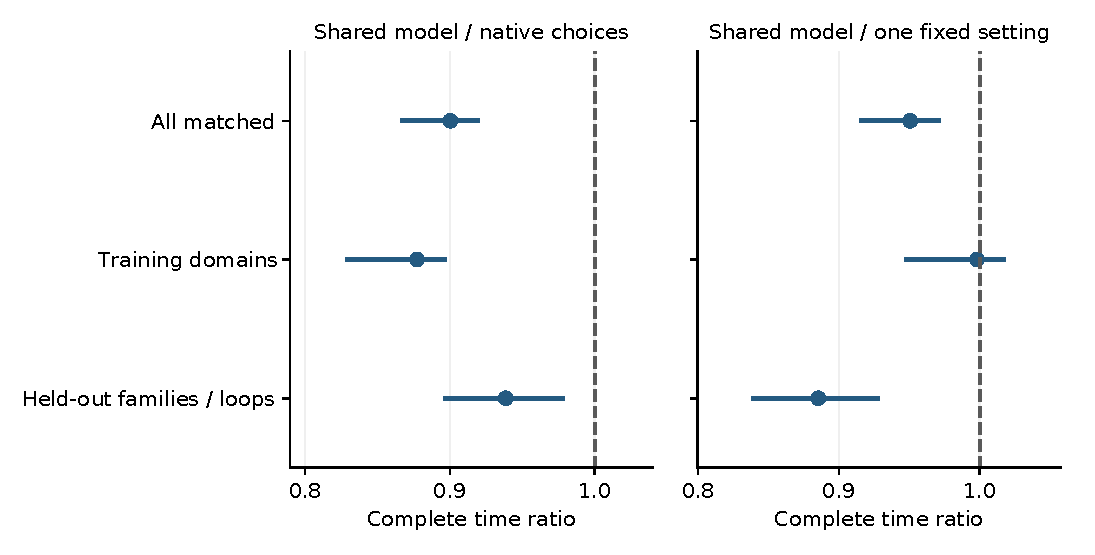
\includegraphics[width=\linewidth]{paper_figures/general_policy_times.pdf}
\caption{Complete time of the corrected shared model, separated into training domains and physical holdouts. Both controls use the same exact implementation. The fixed control has one setting for all requests. The line at one marks equal time, and the intervals describe paired repeat variation.}
\label{fig:general-times}
\end{figure}
\begin{figure}[!htbp]\centering
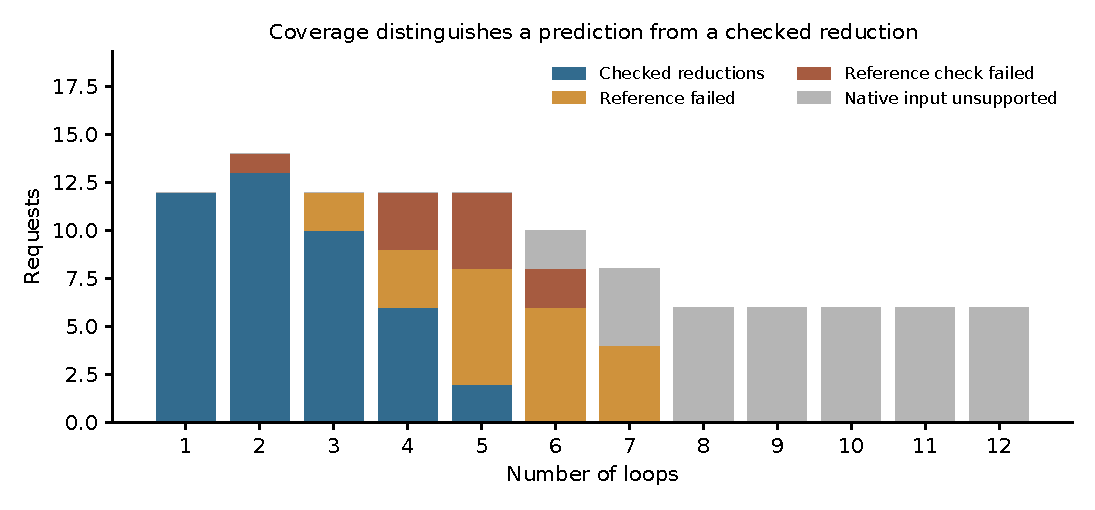
\includegraphics[width=\linewidth]{paper_figures/general_policy_coverage.pdf}
\caption{The loop range extends through twelve, while native completion has a smaller measured range. Predictions for unsupported inputs do not count as reductions. Failed reference checks also prevent a timing claim.}
\label{fig:general-coverage}
\end{figure}
\FloatBarrier
The family holdouts test transfer within this finite set of denominator structures, target powers, and rational parameter values. They do not establish performance for arbitrary graph routings, large target ranks, general symbolic kinematics, cuts, or unbounded loop order. The same physical definitions have also been used in earlier project development, although the excluded groups supply no labels or model-selection costs to this new fit. The high-loop failures and native input limits therefore remain part of the result.

\section{Initial shared-model trial and corrected fitting}
The first shared-model trial uses profile 1201 and records 42 matched requests. Its learned-to-native ratio is 0.829. During an audit of the installed training implementation, we found that the multi-output objective averaged across outputs while its gradient summed them. We changed the objective to the output sum, checked all 17 components of a small-network gradient by finite differences, and refitted using the same original training and validation data. The maximum absolute discrepancy in that check is 1.9e-11. No reserved label enters refitting or model selection. The corrected model is tested on fresh profile 1213, and both trials remain in the evidence record.

\section{Shared structural model, actions, and fitting}
\label{app:shared}
Let $n$ be the number of physical propagators and $E$ the number of independent external momenta. Let $B_{ih}$ be one when loop momentum $\ell_h$ appears in propagator momentum $q_i$, and zero otherwise. Table~\ref{tab:structural-inputs} groups the 27 base inputs. Means run over the target batch unless another set is specified. A weighted incidence multiplies the relevant numerator power or extra denominator power by the corresponding row sum of $B$ before summing over propagators.
\begin{table}[!htbp]\centering\small
\caption{The base structural inputs. Each quantity is computed from the family definition and target indices before Kira generates equations.}
\label{tab:structural-inputs}
\begin{tabularx}{\linewidth}{@{}lYr@{}}\toprule
Group & Quantities & Number\\\midrule
Family dimensions & $L,E,N,n$; number of symbolic invariants & 5\\
Propagator structure & Massive-entry count; coupled-physical-entry count; maximum physical row and column sums of $B$; mean external-momentum incidence over all entries & 5\\
Target batch & Log of one plus target count; number of target sectors & 2\\
Power ranges & Minimum, mean, and maximum extra positive powers and numerator rank & 6\\
Positive indices & Minimum, mean, and maximum number of positive indices & 3\\
Further index limits & Largest absolute index; maximum positive-power sum; maximum number of absent physical denominators & 3\\
Weighted powers & Mean dots on massive entries; mean numerator-weighted and dot-weighted loop incidence & 3\\\bottomrule
\end{tabularx}
\end{table}

We add eight ratios: $N/n$, $n/L$, massive-entry fraction, coupled-physical-entry fraction, maximum dots divided by $n$, maximum rank divided by $N-n$, maximum physical loop incidence divided by $L$, and maximum physical loop degree divided by $n$. Each denominator is replaced by at least one. Six further features are the mean fractions of indices equal to $-2,-1,0,1,2,3$. The final three are $\log[1+L(L+E)]$, $\log(1+n)(1+D_T)$, and $\log[1+\max(1,N-n)](1+R_T)$. These definitions give 44 features. Permuting loop names or entries within the physical and auxiliary groups preserves the pooled counts when the indices are permuted consistently. A change of momentum routing need not preserve them, and identical features need not identify identical reduction problems.

Let $(r_0,s_0,d_0)$ be the target maxima of positive-power sum, numerator rank, and extra positive power. Table~\ref{tab:shared-actions} defines ten candidate actions. Bounds are nonnegative and $r$ is at least the number $t_{\rm top}$ of positive entries in the largest top sector. Kira's subsector restriction uses~\cite{Kira3}
\begin{equation}
 s\leq\max\{1,t-l+1,s_{\max,\mathrm{sector}}\},
 \label{eq:truncation-new}
\end{equation}
where $t$ is that sector's positive-index count, $l$ is the chosen parameter, and the last term is an explicitly assigned sector limit.
\begin{table}[!htbp]\centering\small
\caption{The shared model's candidate seed configurations. Changes are relative to the target maxima. A dash disables the additional subsector restriction.}
\label{tab:shared-actions}
\begin{tabular}{@{}lrrrr@{}}\toprule
Action & $\Delta r$ & $\Delta s$ & $\Delta d_0$ & $l$\\\midrule
Native &0&0&0&---\\
Numerator expansion &0&1&0&---\\
Tight & $-1$&$-1$&$-1$&---\\
Reduced dots &$-1$&0&$-1$&---\\
Reduced numerator rank &0&$-1$&0&---\\
Expanded &1&1&1&---\\
Truncated native &0&0&0&$t_{\rm top}-s_0$\\
Truncated expansion &0&1&0&$t_{\rm top}-s_0$\\
Truncated reduced dots &$-1$&0&$-1$&$t_{\rm top}-s_0$\\
Relaxed truncation &0&0&0&$t_{\rm top}-s_0-1$\\\bottomrule
\end{tabular}
\end{table}

For request $c$ and action $a$, define the cost label $y_{ca}=\log(T_{ca}/T_{c0})$, with native action $0$. Because the denominator is positive and independent of $a$, and the logarithm is increasing, minimizing the unmodified label selects the action with the least recorded time. Training clips this label to $[-4,5]$ after assigning failures at least 180 seconds or three times the measured attempt cost, whichever is larger. Clipping limits extreme labels and can merge their order; the validation comparison therefore uses the recorded costs directly.

The neural regression model uses composed affine maps and componentwise activations~\cite{Pedregosa2011Bounds}. The selected network standardizes each feature by its training mean and standard deviation, with a minimum scale of $10^{-6}$. With standardized vector $z$, its outputs are defined by
\begin{equation}
 h_1=\operatorname{ReLU}(W_1^{\mathsf T}z+b_1),\quad
 h_2=\operatorname{ReLU}(W_2^{\mathsf T}h_1+b_2),\quad
 \widehat y=W_3^{\mathsf T}h_2+b_3,
 \label{eq:network-new}
\end{equation}
where $\operatorname{ReLU}(u)=\max(0,u)$ acts on each component. Both hidden vectors have 48 components and the output has ten components, one per action. We fit squared prediction error with a squared-weight penalty of strength 0.1 using the regression implementation of Ref.~\cite{Pedregosa2011Bounds}. For $n_{\rm tr}$ training requests, the corresponding objective is
\begin{equation}
 \mathcal L=\frac{1}{2n_{\rm tr}}\sum_{c,a}
 (\widehat y_{ca}-y_{ca})^2+
 \frac{0.1}{2n_{\rm tr}}\sum_j\|W_j\|_F^2.
 \label{eq:loss-new}
\end{equation}
To motivate the first term, assign a formal residual $e_{ca}=\widehat y_{ca}-y_{ca}$ the density $p(e)=(2\pi)^{-1/2}\exp(-e^2/2)$. Then
\begin{equation*}
 -\frac{1}{n_{\rm tr}}\log\prod_{c,a}p(e_{ca})
 =\frac{1}{2n_{\rm tr}}\sum_{c,a}e_{ca}^2+\frac{10}{2}\log(2\pi).
\end{equation*}
Removing the constant and adding the stated quadratic penalty gives Eq.~\eqref{eq:loss-new}. This construction motivates a regression objective; the study does not infer a Gaussian distribution of timing errors.

The candidate set also contains trees, random forests, and extremely randomized forests at depths 2, 4, and 7, with at least three samples per leaf; forests contain 48 trees~\cite{CART1984,Breiman2001Forest,Geurts2006ExtraTrees}. Two ridge fits use regularization strengths 1 and 10, and the neural candidates have two hidden layers of either 24 or 48 components. Neural fitting uses L-BFGS with at most 500 iterations~\cite{Pedregosa2011Bounds}. The initial implementation exposed an inconsistent scaling between the installed multi-output loss and its gradient. We corrected the loss to match the summed-output gradient, checked it by finite differences, and refitted using the same training and validation inputs. The initial comparison remains in the notes; the corrected model uses a new reserved profile. Candidate convergence warnings remain recorded, and no fit certifies a global optimum.

For every candidate, five-fold cross-validation withholds whole ordered graph structures, with feature scaling fitted within each training fold. The separate validation set selects a single fixed action. We compare that action and native bounds as global anchors, with margins $0,0.05,0.12,0.25$. If $b$ is the anchor and $a_* =\arg\min_a\widehat y_a$, the policy changes to $a_*$ only when $\widehat y_{a_*}<\widehat y_b-\eta$. Exponentiation gives the predicted ratio condition $\exp(\widehat y_{a_*}-\widehat y_b)<\exp(-\eta)$. We select the candidate minimizing the worse of its grouped-fold and separate-validation ratios to native cost. This rule is fixed before the reserved test. A score below 0.97 permits default deployment; it is evidence from validation, not a guarantee for future inputs.

The selected candidate is the 48-component network, with action 7 from Table~\ref{tab:shared-actions} (numbered from zero) as anchor and margin 0.05. Training uses only historical training records after the physical holdouts. Their historical timers differ in whether initial imports are included; all new reserved controls use the same complete fresh-process timer. The training record contains every source and model candidate. A failed new seed attempt retries native and expanded bounds with duplicate configurations removed. The shared model never uses target coefficients or measured test time as an input.

\section{Physical inputs and the loop-order test}
\label{app:families-new}
The following equations define the physical inputs for our benchmark families. All denominators follow Eq.~\eqref{history:eq:family}. Let $Q=\sum_{i=1}^{L}\ell_i$. For $L\geq2$, the vacuum families contain
\begin{equation}
 q_i=\ell_i\quad(1\leq i\leq L),\qquad q_{L+1}=Q.
 \label{eq:vacuum-new}
\end{equation}
The one-mass case gives only the final entry a nonzero mass; the massive case assigns distinct nonzero masses to all physical entries. The one-loop vacuum is a single massive tadpole. The two-point families replace the final momentum by $p-Q$, with either all zero masses or distinct nonzero masses. Their single independent external invariant is $p^2$.

For the four-point families, choose massless external momenta with $p_1+p_2+p_3+p_4=0$, and write $P=p_1+p_2$, $U=p_1+p_2+p_3$, $s=P^2$, $t=(p_2+p_3)^2$. Expanding these squares gives $2p_1\cdot p_2=s$, $2p_2\cdot p_3=t$, and $2p_1\cdot p_3=-s-t$. The physical momenta of the $L$-loop ladder are
\begin{equation}
 \{\ell_i,\ell_i-P:1\leq i\leq L\} \cup\
 \{\ell_i-\ell_{i+1}:1\leq i<L\}\ \cup\
 \{\ell_1-p_1,\ell_L-U\}.
 \label{eq:ladder-new}
\end{equation}
We order the loop momenta first, the $P$-shifted momenta next, then adjacent differences, and finally the two end entries. The box with bubble subgraphs has
\begin{equation}
 (q_1,q_2,q_3,q_4)=(\ell_1,\ell_1-p_1,\ell_1-P,\ell_1-U),\qquad
 (q_{2j+1},q_{2j+2})=(\ell_j,\ell_j-\ell_1),\quad 2\leq j\leq L.
 \label{eq:bubbles-new}
\end{equation}
All these four-point propagators are massless. This box family has bubble subgraphs and is a restricted connected scattering class.

The additional massless nonplanar box uses the routing of Ref.~\cite{KiraOriginal}:
\begin{align}
 (q_1,\ldots,q_9)=(&\ell_1,\ell_2,p_1-\ell_1,p_2-\ell_2,
 p_1+p_2-p_3-\ell_1,\nonumber\\
 &p_1-\ell_1+\ell_2,p_1-p_3-\ell_1+\ell_2,
 \ell_1-p_3,\ell_2-p_1-p_2).
 \label{eq:nonplanar-new}
\end{align}
Its first seven entries are physical. Here the outgoing-momentum convention gives $p_i^2=(p_1+p_2-p_3)^2=0$, $s=(p_1+p_2)^2$, and $t=(p_1-p_3)^2$. Expansion gives $2p_1\cdot p_3=-t$ and $2p_2\cdot p_3=s+t$. The pentagon uses five massless external momenta with zero sum and physical momenta $\ell$, $\ell-p_1$, $\ell-p_1-p_2$, $\ell-p_1-p_2-p_3$, and $\ell-p_1-p_2-p_3-p_4$. Adjacent invariants are $s_{ij}=(p_i+p_j)^2$. Squaring complementary momentum sums gives, for example, $2p_1\cdot p_3=s_{45}-s_{12}-s_{23}$. The box with one virtual external leg uses $(\ell,\ell-p_1,\ell-p_1-p_2,\ell-p_3)$, with $p_i^2=0$ for $i=1,2,3$ and $v=(p_1+p_2-p_3)^2$; its remaining product is $2p_2\cdot p_3=s+t-v$.

There are $L$ loop squares, $L(L-1)/2$ products of distinct loop momenta, and $LE$ loop--external products. Adding these counts gives the complete coordinate number
\begin{equation}
 N=\frac{L(L+1)}2+LE.
 \label{eq:count-new}
\end{equation}
This is the representation used by Kira~\cite{Kira3}. We append squared momentum differences when their scalar-product coefficient vectors increase the exact rank, until all $N$ coordinates are independent. The candidate order follows loop momenta and then external momenta. Auxiliary indices are nonpositive. The tested interface admits at most 31 coordinates; this is an implementation limit, not an upper bound on the mathematics of IBP. It permits the defined vacuum inputs through seven loops, two-point inputs through six, and four-point inputs through five. Completion remains a separate test.

For the final fresh profile $h=1213$, choose $m_{\rm one}^2=2h+17$, $m_i^2=2h+19+6(i-1)$, $p^2=-2h-29$, $s=-1009-12h$, and $t=-1021-14h$, using only the variables required by each of the six recursive families. All values use a common squared-momentum unit. Additional scattering profiles follow the explicit assignments in Table~\ref{tab:extra-kinematics}. The independent reference increases the target's positive-power, numerator, and dot limits by one; the check increases the numerator allowance once more and changes integral ordering. Every checked reference and every failure is retained.
\begin{table}[!htbp]\centering\small
\caption{Additional scattering kinematics at profile $h=1201$ for the initial shared-model trial and $h=1213$ for the corrected-model test. These expressions define the chosen inputs in a common squared-momentum unit.}
\label{tab:extra-kinematics}
\begin{tabularx}{\linewidth}{@{}lY@{}}\toprule
Family & Invariants\\\midrule
Nonplanar box & $s=-113-18h$, $t=-127-10h$\\
Box with virtual leg & Same $s,t$; $v=-149-12h$\\
Pentagon & $(s_{12},s_{23},s_{34},s_{45},s_{51})=(-11,-13,-17,-19,-23)-20h(1,1,1,1,1)$\\\bottomrule
\end{tabularx}
\end{table}


Let $a_i^{(0)}=1$ on the $n$ physical entries and zero otherwise. For $j=0,\ldots,\min(n,3)-1$, set $i_j=1+[(h+j)\bmod n]$ and, when $N>n$, $k_j=n+1+[(h+j)\bmod(N-n)]$. The dotted batch uses $\boldsymbol a^{(0)}+2\boldsymbol e_{i_j}$; the mixed batch uses $\boldsymbol a^{(0)}+\boldsymbol e_{i_j}-\boldsymbol e_{k_j}$. Without an auxiliary entry, the latter has only the extra physical power. The three additional structures use the earlier generator, which puts a second physical dot on the next entry when no auxiliary entry exists. The notes give its full historical target definitions. These are indexed Feynman integrals whose reductions come from exact Kira calculations.

For the retained two-loop sparse-seed test, the planar box has physical momenta $(\ell_1,\ell_1-p_1,\ell_1-p_1-p_2,\ell_2,\ell_2-p_1-p_2,\ell_2-p_1-p_2-p_3,\ell_1-\ell_2)$ and auxiliary momenta $(\ell_1-p_3,\ell_2-p_1)$. Its convention is $2p_1\cdot p_2=s$, $2p_1\cdot p_3=t$, and $2p_2\cdot p_3=-s-t$. The nonplanar family is Eq.~\eqref{eq:nonplanar-new}. Both use unit physical powers and numerator ranks two through four on one or two auxiliary entries. The equation-transfer comparison also includes the three-loop vacuum with momenta $(\ell_1,\ell_2,\ell_3,\ell_1-\ell_2,\ell_2-\ell_3,\ell_1-\ell_3)$ and the massive two-point ladder $(\ell_1,\ell_1-p,\ell_2,\ell_2-p,\ell_3,\ell_3-p,\ell_1-\ell_2,\ell_2-\ell_3,\ell_1-\ell_3)$, whose final entry is auxiliary. For the three-loop vacuum the squared masses are $(1,1,1,13,13,53+2h)$; for the two-point ladder they are $(1,0,0,0,0,0,0,0)$ on the physical entries, with $p^2=-1009-12h$. The earlier sparse-seed fit uses profiles $h=831,832$ for training, $841,842$ for validation, and $851,852$ for the 20-request test. Its planar invariants are $(-1009-12h,-1021-14h)$ and its nonplanar invariants are $(-113-18h,-127-10h)$. A single-direction numerator carries rank two, three, or four; a distributed numerator splits rank three or four into its ceiling and floor halves on the two auxiliary entries. The equation-filter training uses profiles $511,512$, validation uses $513$, and its new-index comparison uses $605,606$. The notes preserve the complete finite target enumeration and source records for those earlier experiments.

\section{Timing ratios and uncertainty}
\label{app:statistics}
Let $T_{cmj}$ be the elapsed time for request $c$, method $m$, and repetition $j$. For the matched set $\mathcal C$, define
\begin{equation}
 S_m=\sum_{c\in\mathcal C}\operatorname{median}_j T_{cmj},\qquad
 R_{m/b}=\frac{S_m}{S_b},\qquad
 \text{time saving}=100(1-R_{m/b})\%.
 \label{eq:timing-new}
\end{equation}
The sum describes that fixed workload. Subtracting $S_m$ from the baseline total $S_b$ and dividing by $S_b$ gives the saving formula; its speedup factor is $S_b/S_m=1/R_{m/b}$. A matched request must complete the compared methods and repetitions with exact agreement. We also report all excluded requests, so these ratios are conditional on completion.

For the new test, we resample the three paired repetition indices within each request 2,000 times, recompute its medians and the ratio of totals, and take the 2.5 and 97.5 percentiles. This applies the bootstrap principle~\cite{Efron1979} to the measured repetition pairs. The interval describes variation on this fixed workload, with limited resolution from three repeats. It does not give a confidence guarantee for unseen integral families or arbitrary loop order. Training, reference discovery, and unsuccessful comparisons are reported separately from matched supplied-basis times.

\section{Reducing preparation failures}
\label{sec:preparation}
The shared-model result separates two costs that require different changes. Its supplied-basis calls complete, while some initial reference calculations or enlarged-region checks fail. We therefore change the preparation workflow and train a second model on individual successful and failed attempts. This comparison includes basis lookup or discovery, both exact reductions, prediction, recovery, and process exit.

The compact workflow first looks for previously checked master indices with the same ordered propagator structure and zero-mass pattern. It reuses these indices while recomputing all coefficients at the new kinematic values. Without a stored basis, it begins with a compact seed region and treats the resulting basis as provisional. A second reduction uses that basis and a different integral ordering, and its coefficients must agree exactly. Kira's supplied-basis check rejects additional masters~\cite{Kira3}. Agreement checks the requested reductions; it does not prove that the provisional basis has the globally smallest possible number of masters. Incomplete attempts expand the seed region, and duplicate attempts are removed.

The new model takes the same 44 structural quantities as the neural model, together with the three seed bounds, the truncation flag and level, the presence and size of a supplied basis, and the integral-ordering setting. Its 52 inputs predict log attempt time and a failure score. We fit random forests and extremely randomized forests~\cite{Breiman2001Forest,Geurts2006ExtraTrees} and select the action with the smallest sum of predicted time and a validation-selected failure penalty. Appendix~\ref{app:risk} defines the outputs and objective. The failure score ranks actions; it is not a calibrated probability.

Training uses 1,405 earlier attempts, including 389 failures, and 58 separate validation requests select the model. The selected random forest has 32 trees of maximum depth 6 and uses a 120-second failure penalty. Fitting and model selection take 3.67 seconds, excluding the earlier cost of collecting labels. Training includes the initial shared-model trial, but excludes the distinct-mass vacuum family, nonplanar boxes, pentagons, and loop orders six and above. The new physical profile supplies no fitting or selection labels.

The reserved comparison contains 33 requests at one through seven loops, using the physical definitions in Appendix~\ref{app:families-new} with profile $h=1237$. It compares expanded discovery and its enlarged-region check with three versions of the compact workflow: native bounds, the frozen neural model, and the cost-and-risk model. Each method receives the same 110-second request deadline and a 60-second cap per native call. Every first attempt is retained, and each initially successful method receives two further repetitions. All four methods use the same 128-bit integral-ordering labels, which Kira supports~\cite{Kira3}; this setting changes the internal ordering representation rather than the exact coefficient arithmetic. The 31-coordinate interface limit remains.

\begin{table}[!htbp]\centering\small
\caption{Preparation outcomes over the full reserved set. The first-pass timer includes successful and unsuccessful requests. Failed-attempt time counts the unsuccessful native calls within that pass. These totals describe work performed; a shorter failed request is not a successful speedup.}
\label{tab:preparation-coverage}
\begin{tabularx}{\linewidth}{@{}Yrrrr@{}}\toprule
Method & First complete & All 3 complete & First pass (s) & Failed calls (s)\\\midrule
Expanded discovery & 17/33 & 16/33 & 1041.6 & 684.2\\
Compact, no ML & 23/33 & 23/33 & 757.8 & 573.1\\
Compact, neural model & 23/33 & 23/33 & 869.0 & 663.4\\
Compact, cost and risk & 23/33 & 23/33 & 895.1 & 677.6\\
\bottomrule\end{tabularx}\end{table}

\begin{table}[!htbp]\centering\small
\caption{Preparation completions by loop order. Each entry requires all three repetitions. The compact columns use the same reuse and checking procedure with the stated decision rule. These results are separate from the earlier supplied-basis coverage in Table~\ref{tab:general-coverage}.}
\label{tab:preparation-loops}
\begin{tabular}{@{}rrrrrr@{}}\toprule
Loops & Requests & Expanded & Compact native & Neural & Cost and risk\\\midrule
1 & 4 & 4 & 4 & 4 & 4\\
2 & 7 & 6 & 7 & 7 & 7\\
3 & 4 & 3 & 3 & 3 & 3\\
4 & 6 & 2 & 3 & 3 & 3\\
5 & 6 & 1 & 4 & 4 & 4\\
6 & 4 & 0 & 2 & 2 & 2\\
7 & 2 & 0 & 0 & 0 & 0\\
\bottomrule\end{tabular}\end{table}

\begin{table}[!htbp]\centering\small
\caption{Complete preparation time on matched requests. Every included method completes all three repeats in the same master-index basis with exact coefficient agreement. The compact/native comparison includes reuse and the changed check; the two ML comparisons isolate prediction within that workflow.}
\label{tab:preparation-times}
\begin{tabularx}{\linewidth}{@{}Yrrr@{}}\toprule
Comparison & Matched & Time ratio & Repeat interval\\\midrule
Compact without ML / expanded & 13 & 0.305 & [0.290,0.329]\\
Neural model / compact without ML & 22 & 0.982 & [0.959,1.021]\\
Cost and risk / compact without ML & 22 & 1.635 & [1.604,1.700]\\
Cost and risk / neural model & 23 & 1.536 & [1.471,1.595]\\
\bottomrule\end{tabularx}\end{table}

The analysis performs 6,375 coefficient comparisons across the repeated and competing outputs. The reused index cache contains 24 earlier checked structures. Their retained discovery and check records cost 341.3 seconds before this experiment; failed attempts during the earlier search add further cost. The compact timings therefore describe use of an existing cache, not cost-free master discovery. In the earlier supplied-basis experiment, 129 neural-model native attempts contain 0 failures. This audit locates the larger failure cost in preparation.

\begin{figure}[!htbp]\centering
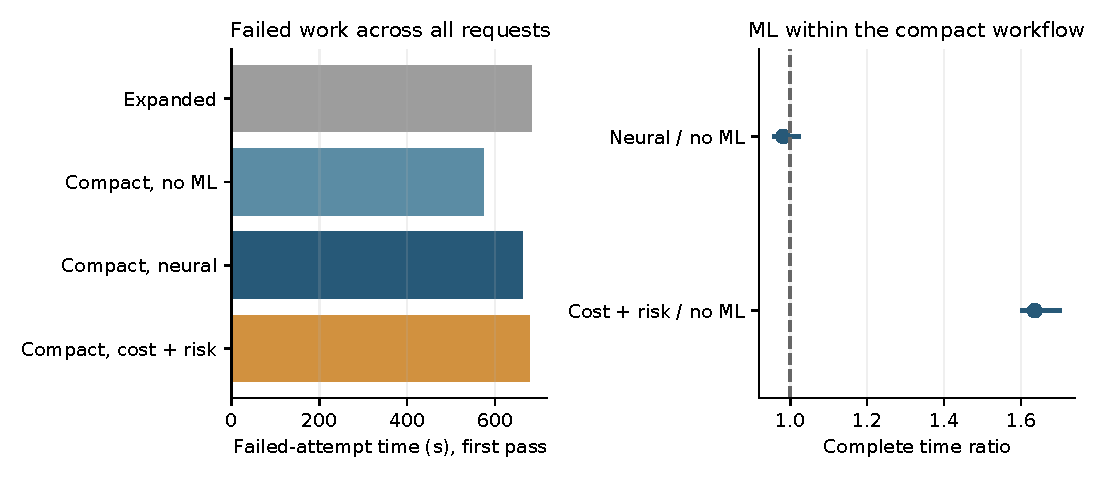
\includegraphics[width=\linewidth]{paper_figures/preparation_results.pdf}
\caption{The preparation comparison keeps failed work and the added ML effect separate. The left panel includes failed calls from every first request. The right panel uses only exact matched completions and compares both models with the same compact workflow without ML. The dashed line marks equal time.}
\label{fig:preparation}
\end{figure}
\FloatBarrier

Compact preparation without ML compared with expanded discovery gives ratio 0.305 on 13 matched requests, with repeat interval [0.290,0.329]. The neural model within compact preparation gives ratio 0.982 on 22 matched requests, with repeat interval [0.959,1.021]. The cost-and-risk model within compact preparation gives ratio 1.635 on 22 matched requests, with repeat interval [1.604,1.700]. The cost-and-risk model increases time in this broad comparison. The neural preparation result also remains consistent with equal time. We keep the failure model and its records for analysis, while the shared neural model remains the validated supplied-basis default.

The full application first checks whether the restricted scalar massless formula applies. This is a physical condition, independent of measured time. Among the remaining requests, the neural preparation model gives ratio 0.985 on 21 matched completions, with repeat interval [0.963,1.025], relative to compact preparation without ML. These measurements do not meet both conditions for retaining learned preparation: a time interval below one and completion of every request completed by its native control. The default therefore uses native choices for preparation and retains the shared neural model for supplied-basis reduction, where the separate test establishes a gain. This deployment choice follows the candidate comparisons. The reported ratios belong to the frozen methods; they do not provide a new independent timing test of the resulting selector.

\subsection{Recovery from an incomplete stored basis}
The first compact trial exposed a target-dependent basis mismatch: a basis checked for earlier targets can omit masters needed by a new batch. The revised application discards a rejected cached basis after expanded seeding also fails, rediscovers without that constraint, and checks the result. It also permits an expanded target check when smaller checks fail. All steps remain inside the same 110-second request budget. A focused follow-up uses six fresh requests at two through five loops and keeps the models and index cache fixed. All three repetitions complete on 6/6 requests with ML disabled, 6/6 with the neural model, and 6/6 with the cost-and-risk model. The neural model gives a ratio of 0.783 on 6 matched requests, with repeat interval [0.743,0.797], relative to the revised workflow without ML. The cost-and-risk model gives a ratio of 0.801 on 6 matched requests, with repeat interval [0.772,0.857], relative to the revised workflow without ML. The comparison passes 2,352 coefficient checks. It tests the recovery change on fresh parameters of selected structures and does not replace the broad trial.

\section{Learning attempt cost and failure risk}
\label{app:risk}
For recorded attempt $i$, let $t_i$ be its elapsed time in seconds and $f_i$ be one if it fails and zero otherwise. We define the two regression targets as $u_i=\log\max(0.001,t_i)$ and $v_i=3f_i$. A tree leaf predicts the mean of each target; averaging the trees gives predictions $\widehat u$ and $\widehat v$~\cite{Breiman2001Forest}. The factor three gives the failure output more weight in the two-output squared-error split objective. For $n$ attempts, that objective is proportional to
\begin{equation}
 \sum_{i=1}^n\bigl[(\widehat u_i-u_i)^2+(\widehat v_i-3f_i)^2\bigr].
 \label{eq:risk-fit}
\end{equation}
To obtain the leaf means, differentiate each sum of squared residuals with respect to its constant leaf prediction. The derivatives are $2\sum_i(\widehat u-u_i)$ and $2\sum_i(\widehat v-3f_i)$; setting them to zero gives the two sample means. Equation~\eqref{eq:risk-fit} is the chosen fitting objective, without an assumption that every failure has the same physical cause.

The runtime score for candidate action $a$ is defined as
\begin{equation}
 C_a=\exp[\operatorname{clip}(\widehat u_a,-5,8)]
       +\lambda\operatorname{clip}(\widehat v_a/3,0,1).
 \label{eq:risk-score}
\end{equation}
Here $\operatorname{clip}(z,l,h)=\min(h,\max(l,z))$ and $\lambda$ has units of seconds. The exponential reverses the log-time target, and division by three reverses the failure-label scaling. Their sum defines a time-based ranking with a failure penalty; it is not a calibrated expected-time estimate. Without a supplied basis, candidate actions exclude the three settings that reduce dot or numerator bounds below the native target limits. All ten settings are available when a basis is supplied.

We compare 32-tree random and extremely randomized forests at depths four and six, with at least five training attempts per leaf~\cite{Breiman2001Forest,Geurts2006ExtraTrees}. Each candidate is evaluated with $\lambda\in\{0,20,60,120\}$ seconds. For each validation request, it chooses one recorded action. Model selection minimizes
\begin{equation}
 V=\frac{\sum_c T_{c,a(c)}+60\sum_c f_{c,a(c)}}{\sum_c T_{c,0}},
 \label{eq:risk-selection}
\end{equation}
where $T$ is the earlier complete action cost including its recovery, $f$ records failure of that action's first attempt, and action zero uses native bounds. Unsuccessful complete validation records receive a 180-second penalty. The denominator is independent of the candidate, so minimizing $V$ minimizes the penalized numerator. The extra 60 seconds deliberately emphasizes avoiding a failed first action even when recovery already contributes to $T$. The model, penalty, and basis cache are fixed before the reserved comparison.

The new grid contains one target shape per selected family and loop order: dotted targets at odd orders and mixed targets at even orders, as defined in Appendix~\ref{app:families-new}. The one-mass vacuum uses orders 1, 2, 4, 5, 6, 7; the distinct-mass vacuum uses 2, 4, 5, 6, 7; each two-point class uses 2 through 6; the ladder uses 1 through 5; and the box with bubbles uses 2 through 5. The nonplanar box, pentagon, and box with one virtual leg add three requests. The cache uses only the master indices from the earlier profile 1201. Stored coefficients never enter prediction or the new reduction. Its structure key distinguishes the ordered momenta and zero versus nonzero mass and invariant assignments. A matching key is only a proposed basis: the new exact calculations must establish target reduction at the new parameters.

Every initially successful method receives three measurements. A paired time ratio includes only requests that complete all three repeats for both methods, use the same master-index set, and agree coefficient by coefficient. Repetition and cross-method checks use exact rational simplification. Different provisional bases, incomplete repetitions, and failed requests remain in the outcome records without a matched ratio. This makes the time comparison conditional on equal completed work.

The focused recovery comparison uses profile $h=1249$ for the distinct-mass vacuums at four and five loops, the massless and massive three-loop two-point families, the three-loop box with bubbles, and the two-loop ladder. It uses dotted targets at odd orders and mixed targets at even orders. Three repetitions compare the same compact workflow with native bounds, the neural model, and the cost-and-risk model. Model weights and cache entries are unchanged. The revised recovery rule follows the basis rejection observed in the preceding experiment; this follow-up therefore tests that specific correction.

% END CURRENT WORKFLOW UPDATE
% BEGIN CURRENT WORKFLOW UPDATE
% THIRTEEN LOOP EXTENSION
\section{Exact loop blocks and learned costs through thirteen loops}
\label{sec:blocks13}
The next extension changes the calculation around the learned choice. When the active propagators and numerators divide the loop momenta into independent blocks, we reduce each distinct block once and keep the product of its master expansions in factored form. Shared external momenta do not prevent this separation. An active numerator that joins two loop sets prevents their separate reduction. Appendix~\ref{app:blocks13} derives the factorization and gives exact tadpole, one-mass vacuum, and massless two-point formulas used before native Kira. These routes use mathematical identities and make no learned choice.

The remaining blocks use the same 44 structural inputs and ten seed actions as the shared model. We fit eleven new candidates on all 111 available historical training requests, with 76 separate validation requests. They comprise six forests, two regularized linear regressions, and three neural networks. The forests follow the random-forest and extremely randomized-tree methods~\cite{Breiman2001Forest,Geurts2006ExtraTrees}. Each forest averages its tree predictions. The cost labels sum the native attempts and their recovery cost, since a checked stored basis permits a single production reduction. An unsuccessful full action receives a penalty. The first selection retains the preceding network with two 48-component hidden layers. After adding the two exact convolution formulas, we compare the fitted candidates again on the historical validation requests that still need native Kira, and retune the fixed control on the same requests. This final selection precedes the corrected reserved test. The notes give the candidate settings and selection rules.

A stored basis contains integral indices, and Kira recomputes coefficients at the current parameters. During development, combining several alternative preferred master lists allowed different seed actions to return different bases. Their coefficients could not be compared entry by entry. We therefore reduce all stored preferred indices at separate development parameters and retain one checked master set per structure. A production result must use this set; otherwise the application retries with less restrictive seeds. Unknown structures require master discovery and a second exact calculation. These preparation costs remain outside the supplied-cache timing and are recorded separately in the notes.

The first reserved grid contains 79 coupled-family requests and 52 independent-block requests through thirteen loops. It records every failure and native input limit. After the basis correction, we use new parameter profiles for the coupled and product tests. Each product uses one- or two-loop blocks; a total of thirteen loops therefore tests the exact composition and its local learned decisions. It does not test a general irreducible thirteen-loop matrix. Further sets check the derived one-mass vacuum and massless two-point formulas with scalar targets and one quadratic numerator. The notes give the initial grid and all outcomes, while Table~\ref{tab:blocks13} gives the corrected application's paired results.

All three corrected methods share the block construction, exact formulas, checked basis, and recovery limits. The native method uses native seed bounds. The fixed method uses the preselected common action. The learned method predicts an action from the block structure. Each timing starts a fresh process and includes prediction, native equation generation, reduction, recovery, output, and exact comparison with an independent reference. Three repetitions rotate method order. Reference preparation is separate. A time ratio uses only requests for which both methods complete all three exact checks; incomplete requests remain in the coverage counts. Analytic-only requests contribute no evidence for ML.

The final validation comparison contains 58 requests that need native Kira and 18 requests handled by the exact formulas. It selects a 48-tree extremely randomized forest with maximum depth 10, with decision margin 0.0. The model weights and decision rule remain fixed throughout the corrected reserved tests.

The corrected grid contains 92 requests. The learned route completes all three exact checks on 91 of them, with 0 first-run completions that lack matching reference coefficients. Across all methods, the experiment records 892 timed attempts and 38012 coefficient comparisons.

\begin{table}[!htbp]\centering\small
\caption{Corrected application: paired time ratios on completed requests. The numerator is the learned application time; the controls share all exact changes. Times are sums of request medians in seconds. Each row has its own matched set. Analytic rows execute the same formula code and contain no ML inference. These are measurements of this study.}
\label{tab:blocks13}
\begin{tabularx}{\linewidth}{@{}Yrrrr@{}}\toprule
Comparison & Requests & Control & Learned & Ratio\\\midrule
Coupled families / native & 18 & 27.400 & 22.715 & 0.829\\
Coupled families / fixed & 18 & 22.471 & 22.715 & 1.011\\
Independent blocks / native & 52 & 187.116 & 189.802 & 1.014\\
Independent blocks / fixed & 52 & 191.693 & 189.802 & 0.990\\
Vacuum formula / native & 11 & 12.441 & 11.300 & 0.908\\
Vacuum formula / fixed & 11 & 11.735 & 11.300 & 0.963\\
Massless formula / native & 10 & 10.895 & 10.796 & 0.991\\
Massless formula / fixed & 10 & 10.866 & 10.796 & 0.994\\
\bottomrule\end{tabularx}\end{table}
\begin{figure}[!htbp]\centering
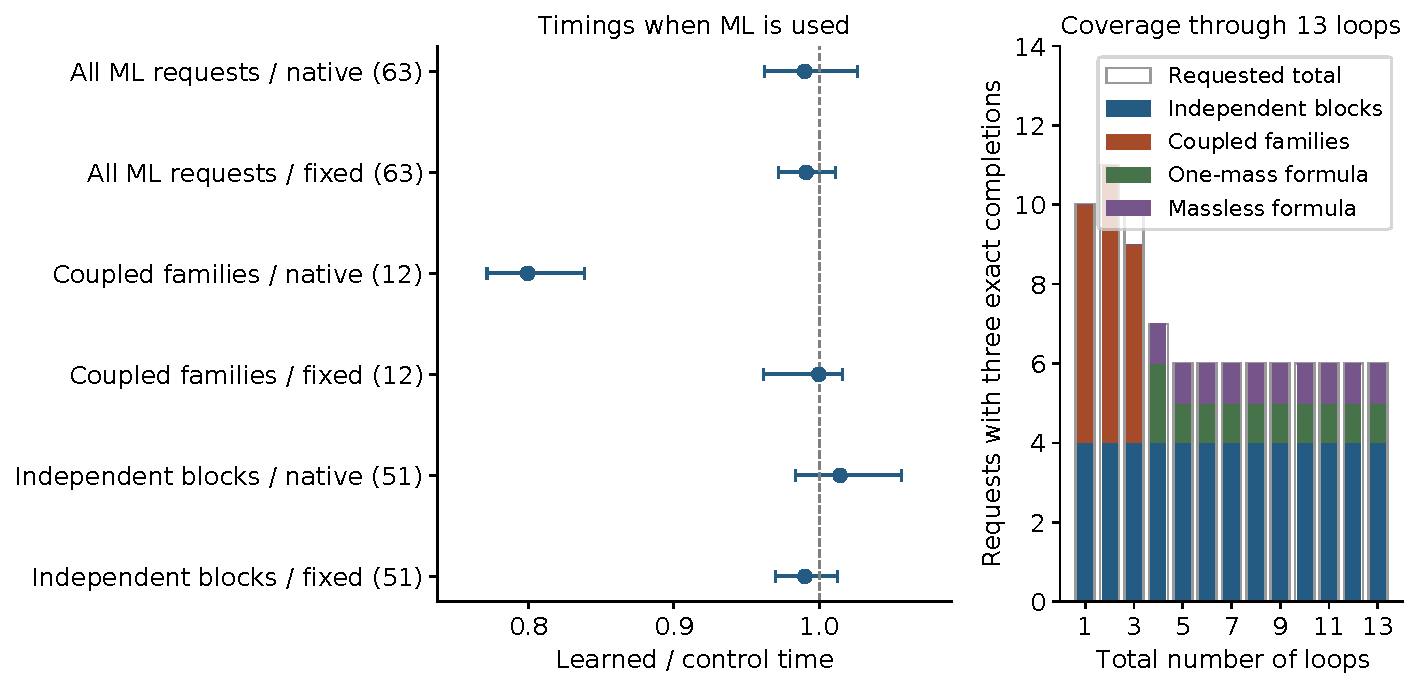
\includegraphics[width=\linewidth]{paper_figures/factorized_results.pdf}
\caption{Left: only requests that invoke ML are included, and the controls share all exact changes. The comparisons with fixed choices include equal time within repetition variation. Intervals describe the three repetitions. Counts in parentheses identify matched requests. Right: completion depends on the integral structure. High-loop products contain small independent blocks, while each analytic formula applies to its specified denominator structure. The bar outline gives the requested total. These sets do not establish general coupled high-loop coverage.}
\label{fig:blocks13}\end{figure}

On requests that actually invoke ML, the time ratio is 0.990, with repetition interval $[0.963,1.026]$, on 63 matched requests. Against the fixed action on its matched ML requests, the time ratio is 0.991, with repetition interval $[0.972,1.011]$, on 63 matched requests. The comparison with native choices does not resolve a saving beyond repetition variation. The comparison with fixed choices does not resolve a saving beyond repetition variation. These controls isolate the learned seed decision after the exact changes.

The learned method records 45 unsuccessful native attempts among 288 native calls in the timed tests. A completed request includes its failed attempts and recovery in the measured cost. Unverified learned attempts consume 101.255 seconds in addition to the paired completed-request totals. Their outcomes remain in the coverage counts.

Across all timed attempts, the learned application uses 811.364 seconds, native choices use 790.074 seconds, and the fixed choice uses 818.950 seconds. This total includes the unfinished request and all repetitions. The learned application therefore does not reduce total time against native choices on this bounded workload.

In the 63 matched ML requests against the fixed control, the model changes the first native action in 34 requests. The remaining requests retain the fixed action and still pay the prediction cost.

Compared with the initial block application on the matched fresh coupled set, the time ratio is 1.046, with repetition interval $[0.989,1.085]$, on 16 matched requests. On the separate one-mass vacuum targets with a completed initial block reduction, the time ratio is 0.187, with repetition interval $[0.168,0.214]$, on 4 matched requests. For the corresponding massless numerator comparison, the time ratio is 0.781, with repetition interval $[0.724,0.891]$, on 1 matched requests. These changes include exact formulas and revised basis handling, so they do not measure ML alone.

The separate gamma-formula checks cover 14 vacuum requests through thirteen loops and 50 target coefficients. Native Kira confirms 5 of the attempted low-loop requests, with 14 coefficient comparisons; 0 attempted native references do not complete. Higher-loop agreement between the finite-product and gamma expressions checks the derivation and implementation, without establishing a native high-loop timing gain.
\FloatBarrier

The massless numerator checks add 12 requests and 60 gamma comparisons through thirteen loops. Native Kira verifies 3 low-loop requests and 15 coefficients; 0 native references do not complete. These formulas precede ML and provide no evidence for a learned gain.

\section{Initial thirteen-loop grid and the basis correction}
\label{sec:blocks13-initial}
The initial application combined earlier checked preferred master lists into one list per structure. This list could contain alternative basis elements. Different seed regions could then produce different master representations. A failed entrywise coefficient comparison therefore remains unverified; it is not treated as proof that the integral identity is wrong. The corrected application forms one basis by reducing the complete earlier index list on development parameters, checks it independently, and tests new physical profiles. No initial reserved coefficient enters model fitting or basis calibration.

The initial grid uses six coupled-family definitions at each loop order, with the stated one-loop omissions, and three additional scattering structures. It adds four product structures per loop order. Product blocks have at most two loops, share external kinematics, and use distinct loop momenta. An odd loop count adds a one-loop remainder. Unused cross-block scalar-product coordinates have zero target powers. An explicit structural check confirms that an active cross-block numerator joins its blocks.

The 52 product requests use rational profile $h=1307+4L$. The corrected products use $h=1607+4L$. The coupled profiles are 1301 and 1601, and the basis-calibration profile is 1501. The one-mass formula checks use $h=1409+6L$, and the massless numerator checks use $h=1801+6L$. The family equations and parameter rules follow Appendix~\ref{app:families-new}. The scalar vacuum checks raise one massless or the massive denominator by two powers; the numerator checks add one power to one denominator and insert one auxiliary quadratic numerator. Additional three- and four-loop checks use $(2k_1-3k_2+k_3)^2$ as the numerator. The massless checks raise one physical power and include both internal-momentum and external-momentum numerator coordinates. All stated dimension dependence remains symbolic.

\begin{table}[!htbp]\centering\small
\caption{Initial grid: three exactly checked completions and requested totals. These counts retain the basis mismatch and native resource limits.}
\begin{tabular}{rrrrr}\toprule
Loops & Requests & Native & Fixed & Learned\\\midrule
1 & 10 & 10 & 10 & 10\\
2 & 11 & 11 & 10 & 10\\
3 & 10 & 9 & 6 & 6\\
4 & 10 & 8 & 7 & 7\\
5 & 10 & 6 & 5 & 5\\
6 & 10 & 5 & 4 & 4\\
7 & 10 & 5 & 4 & 4\\
8 & 10 & 4 & 3 & 3\\
9 & 10 & 5 & 4 & 4\\
10 & 10 & 4 & 3 & 3\\
11 & 10 & 5 & 4 & 4\\
12 & 10 & 4 & 3 & 3\\
13 & 10 & 5 & 4 & 4\\
\bottomrule\end{tabular}\end{table}
\begin{figure}[!htbp]\centering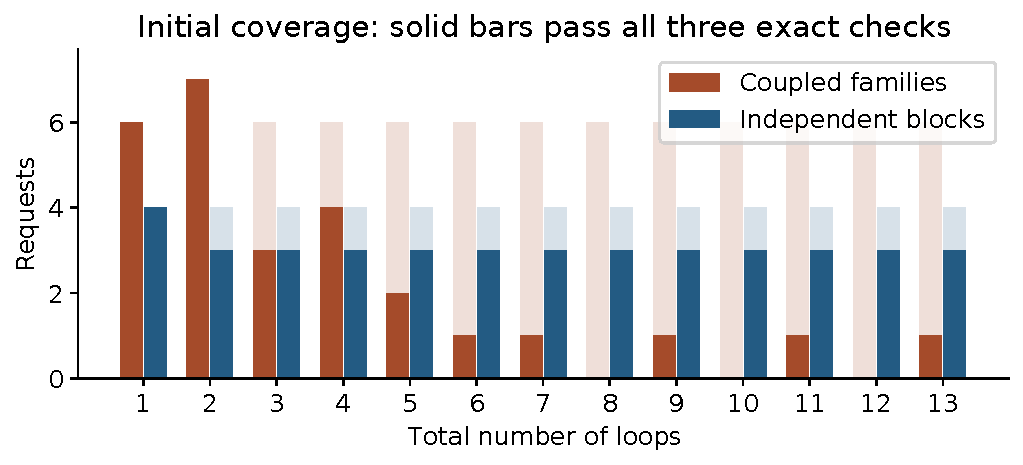
\includegraphics[width=.9\linewidth]{paper_figures/factorized_coverage.pdf}
\caption{Initial grid coverage. Pale bars show requested cases and solid bars show three checked learned completions. Independent products and coupled families have different native requirements.}\end{figure}

The initial grid records 954 timed attempts and 32149 coefficient comparisons. The corrected basis calibration checks 21 structures, with 255.840 seconds summed over the preparation attempts, including failures. Its preparation runs and unsuccessful attempts remain in the stored calibration records. The refitting takes 15.006 seconds and checks 1221 exported predictions against the training library. All eleven new fits remain available. The initial selection retains the prior network; the final selection uses only the remaining native validation workload.

The refit compares 48-tree random forests and extremely randomized forests at depths 3, 6, and 10, with at least three examples per leaf. Ridge penalties are 1 and 10. Neural candidates have two hidden layers of width 24, 48, or 80, regularization 0.3, and a 500-iteration L-BFGS limit. Five folds keep each ordered graph structure in one fold. The candidate score is the larger of the grouped-fold and separate-validation time ratios. Candidate action margins are 0, 0.05, 0.15, and 0.3 relative to either native bounds or the validation-selected fixed action. The best candidate replaces the preceding model only if its validation cost is at least one percent lower and its candidate score is below one.

Each successful training action uses the sum of its native-attempt times, including recovery. Each failed full action uses the larger of 180 seconds and three times that sum. We take the median when a historical action has repeated measurements, divide by the corresponding native cost, take its logarithm, and clip the training label to $[-4,5]$. These are chosen training definitions, not measured test times. The model equations follow Appendix~\ref{app:shared}. The initial retained neural model uses its previously selected margin 0.05. For the corrected application, we remove the validation requests handled by the exact formulas, retune the common fixed action, and compare all saved fitted predictors with anchors at native bounds and that fixed action. We minimize their summed validation cost over the same four margins. A candidate must improve this cost by at least one percent over the preceding policy before it replaces that policy. No reserved coefficient or timing enters this selection.

The initial block interface also has a separate comparison with the previously published application: the time ratio is 0.449, with repetition interval $[0.408,0.454]$, on 26 matched requests. Its requests differ from the corrected experiment, so these ratios cannot be multiplied.

For the corrected interface against the initial block interface on the matched fresh coupled set, the time ratio is 1.046, with repetition interval $[0.989,1.085]$, on 16 matched requests. This comparison includes exact changes and cannot isolate ML.

\begin{table}[!htbp]\centering\small
\caption{Corrected tests by total loop count. Only matched nontrivial requests that invoke ML enter each ratio. Controls share the exact preprocessing. At four loops and above, these ML comparisons use independent products of small blocks. Formula-only requests remain outside this table. A ratio below one means less time with the learned choice.}
\begin{tabular}{rrrrr}\toprule
Loops & Native pairs & Learned/native & Fixed pairs & Learned/fixed\\\midrule
1 & 7 & 1.006 & 7 & 0.974\\
2 & 9 & 1.006 & 9 & 1.012\\
3 & 7 & 0.837 & 7 & 1.003\\
4 & 4 & 1.004 & 4 & 0.980\\
5 & 4 & 1.064 & 4 & 1.059\\
6 & 4 & 1.018 & 4 & 0.958\\
7 & 4 & 1.020 & 4 & 1.030\\
8 & 4 & 1.020 & 4 & 0.996\\
9 & 4 & 1.024 & 4 & 0.964\\
10 & 4 & 0.960 & 4 & 1.001\\
11 & 4 & 0.964 & 4 & 0.936\\
12 & 4 & 1.052 & 4 & 0.983\\
13 & 4 & 1.021 & 4 & 1.007\\
\bottomrule\end{tabular}\end{table}

\section{Independent loop blocks and exact convolution formulas}
\label{app:blocks13}
\subsection{When a product reduction is exact}
Suppose the loop momenta partition into $q$ disjoint sets $B_1,\ldots,B_q$ and every factor with a nonzero exponent depends on loop momenta from one set. External momenta may be shared. Equation~\eqref{history:eq:family} then has the form
\begin{equation}
 I_{\boldsymbol a}=\int\prod_{b=1}^{q}d\mu_b\,f_b
 =\prod_{b=1}^{q}\int d\mu_b\,f_b
 =\prod_{b=1}^{q}I^{(b)}_{\boldsymbol a_b}.
 \label{eq:block-factorization}
\end{equation}
Here $d\mu_b$ contains the normalized loop measures in block $b$, and $\boldsymbol a_b$ selects its active indices. The equality follows first in a convergence domain by iterated integration and then by dimensional analytic continuation, with the convention of Ref.~\cite{Weinzierl2022}. A numerator that contains momenta from two proposed blocks prevents this factorization and joins those blocks in our construction. An unused auxiliary coordinate does not join them.

If block $b$ reduces as $I^{(b)}_{\boldsymbol a_b}=\sum_jr^{(b)}_jM^{(b)}_j$, where $r^{(b)}_j$ are its coefficients and $M^{(b)}_j$ are its masters, substitution into Eq.~\eqref{eq:block-factorization} gives
\begin{equation}
 I_{\boldsymbol a}=\prod_b\left(\sum_jr^{(b)}_jM^{(b)}_j\right).
 \label{eq:factored-expansion}
\end{equation}
This expression retains the complete reduction without distributing the product. Distribution would contain up to $\prod_b n_b$ terms if block $b$ has $n_b$ terms, since each expanded term chooses one entry from each factor. The factored expression stores $\sum_b n_b$ entries. These counts follow from the product construction; they do not claim that an arbitrary coupled integral can be factorized. Identical blocks with identical indices and kinematics require one reduction per request.

\subsection{A massive tadpole}
Let $T_a=\int d^dk/(i\pi^{d/2})(k^2-m^2+i0)^{-a}$. The total derivative of $k^\mu(k^2-m^2)^{-a}$ gives
\begin{equation}
 0=dT_a-2a(T_a+m^2T_{a+1}),\qquad
 T_{a+1}=\frac{d-2a}{2am^2}T_a.
 \label{eq:tadpole13}
\end{equation}
We used $k^2=(k^2-m^2)+m^2$ in the first equality. Repeated substitution reduces each positive integer power to $T_1$. For $m^2=0$, the integral has no scale and vanishes in dimensional regularization~\cite{Weinzierl2022}. This route makes no learned decision.

\subsection{One massive line and massless vacuum lines}
For $L\geq2$, define $Q=\sum_{i=1}^Lk_i$ and
\begin{equation}
 V_{\boldsymbol a,b}=\int\prod_{i=1}^L\frac{d^dk_i}{i\pi^{d/2}}
 \frac{1}{\prod_i(k_i^2+i0)^{a_i}(Q^2-m^2+i0)^b}.
 \label{eq:vacuum13-definition}
\end{equation}
The scalar formula below assumes positive integer $a_i,b$, nonzero $m^2$, and no external momenta. It applies to this denominator structure at any $L$; our checks stop at thirteen loops.

To obtain its index dependence, work first in Euclidean signature. We use analytic continuation in $d$ and the indices before evaluating the integer cases. Define $\Gamma(z)=\int_0^\infty u^{z-1}e^{-u}du$ for $\Re z>0$, with analytic continuation elsewhere. The Schwinger identity and a Gaussian integral give
\begin{align}
 (k_E^2)^{-a}&=\frac{1}{\Gamma(a)}\int_0^\infty dt\,t^{a-1}e^{-tk_E^2},\nonumber\\
 \int\frac{d^dk_E}{\pi^{d/2}}\frac{e^{2ik_E\cdot x}}{(k_E^2)^a}
 &=\frac{1}{\Gamma(a)}\int_0^\infty dt\,t^{a-1-d/2}e^{-x^2/t}
 =\frac{\Gamma(d/2-a)}{\Gamma(a)}(x^2)^{a-d/2}.
 \label{eq:vacuum13-fourier}
\end{align}
The final equality uses $u=x^2/t$ and the defining gamma integral. These parameter and continuation conventions agree with Ref.~\cite{Weinzierl2022}. Put $A_0=\sum_i a_i$ and $\alpha=A_0-(L-1)d/2$. Multiplying the $L$ transforms and inverting them gives the massless convolution proportional to
\begin{equation}
 (Q_E^2)^{-\alpha}\frac{\Gamma(\alpha)}{\Gamma(d/2-\alpha)}
 \prod_i\frac{\Gamma(d/2-a_i)}{\Gamma(a_i)}.
 \label{eq:vacuum13-convolution}
\end{equation}
The transform normalization is independent of the indices and cancels in the ratios used below. The remaining radial integral is
\begin{align}
 \int\frac{d^dQ_E}{\pi^{d/2}}\frac{(Q_E^2)^{-\alpha}}{(Q_E^2+m^2)^b}
 &=\frac{(m^2)^{d/2-\alpha-b}}{\Gamma(d/2)}
 \int_0^\infty\frac{u^{d/2-\alpha-1}}{(1+u)^b}\,du\nonumber\\
 &= (m^2)^{d/2-\alpha-b}
 \frac{\Gamma(d/2-\alpha)\Gamma(\alpha+b-d/2)}{\Gamma(d/2)\Gamma(b)}.
 \label{eq:vacuum13-radial}
\end{align}
The beta integral follows by $v=u/(1+u)$. Combining Eqs.~\eqref{eq:vacuum13-convolution} and \eqref{eq:vacuum13-radial} cancels $\Gamma(d/2-\alpha)$. Wick rotation supplies the relative sign $(-1)^{A_0+b-(L+1)}$ in our Minkowski denominator convention. Let $P=L+1$, $\Delta=A_0+b-P$, and $(z)_n=\Gamma(z+n)/\Gamma(z)$. Dividing by the all-one integral gives
\begin{equation}
 \frac{V_{\boldsymbol a,b}}{V_{\boldsymbol 1,1}}=
 \frac{(-1)^\Delta(m^2)^{-\Delta}
 (P-Ld/2)_\Delta\,[L-(L-1)d/2]_{A_0-L}}
 {(b-1)!\prod_i\left[(a_i-1)!\,(d/2-a_i)_{a_i-1}\right]}.
 \label{eq:vacuum13-scalar}
\end{equation}
Thus the production formula uses finite products, while the independent algebraic check uses the gamma ratios before expansion. If a shifted massless power is zero, its momentum can be integrated after shifting to $Q$, leaving a scaleless factor. If $b=0$, the remaining massless integrals are also scaleless. These terms vanish under the stated assumptions.

\subsection{One quadratic numerator}
The tested extension allows one numerator $v^2$, where $v=\sum_i c_i k_i$ with fixed coefficients $c_i$. We write $V[v^2]$ for Eq.~\eqref{eq:vacuum13-definition} with $v^2$ inserted in the numerator. Define $\beta_i=a_i-d/2$, $\lambda=\sum_i\beta_i$, and
\begin{equation}
 C_v=\left(\sum_i c_i\beta_i\right)^2-\sum_i c_i^2\beta_i^2
 =2\sum_{i<j}c_ic_j\beta_i\beta_j.
 \label{eq:vacuum13-cross}
\end{equation}
This equality is the expansion of the square. In the Fourier representation, a momentum insertion differentiates its corresponding factor in Eq.~\eqref{eq:vacuum13-fourier}. The cross terms give $-C_v(x^2)^{\lambda-1}$, while multiplication of the full convolution by $Q_E^2$ gives
\begin{equation}
 -\frac14\partial_x^2(x^2)^\lambda
 =-\lambda(\lambda+d/2-1)(x^2)^{\lambda-1}.
 \label{eq:vacuum13-laplacian}
\end{equation}
The derivative follows by applying the product rule twice. Dividing these two expressions, then returning to Minkowski signature, yields
\begin{equation}
 V[v^2]=\sum_i c_i^2V_{\boldsymbol a-\boldsymbol e_i,b}
 +\frac{C_v}{\lambda(\lambda+d/2-1)}
 \left(V_{\boldsymbol a,b-1}+m^2V_{\boldsymbol a,b}\right).
 \label{eq:vacuum13-numerator}
\end{equation}
The diagonal term uses $k_i^2$ to cancel one denominator power; the last term uses $Q^2=(Q^2-m^2)+m^2$. Equations~\eqref{eq:vacuum13-scalar} and \eqref{eq:vacuum13-numerator} give rational coefficients in $d$ and $m^2$. Apparent singularities require analytic limits. Higher numerator powers and other vacuum graphs remain outside this formula.

\subsection{Massless two-point integrals with a quadratic numerator}
Let $P=L+1$, $q_i=k_i$ for $i\leq L$, and $q_P=p-\sum_{i=1}^Lk_i$. The massless two-point family is
\begin{equation}
 W_{\boldsymbol a}(p)=\int\prod_{i=1}^L\frac{d^dk_i}{i\pi^{d/2}}
 \prod_{j=1}^{P}(q_j^2+i0)^{-a_j},\qquad p^2\ne0.
 \label{eq:massless13-definition}
\end{equation}
Here all $a_j$ are positive integers. Applying Eq.~\eqref{eq:vacuum13-fourier} to the $P$ massless factors and inverting their product gives the convolution coefficient
\begin{equation}
 \mathcal C(\boldsymbol a)=
 \frac{\Gamma(A-Ld/2)}{\Gamma(Pd/2-A)}
 \prod_{j=1}^P\frac{\Gamma(d/2-a_j)}{\Gamma(a_j)},\qquad A=\sum_j a_j.
 \label{eq:massless13-gamma}
\end{equation}
The momentum power is $Ld/2-A$, as follows either from the inverse transform or from mass dimension. Dividing by the all-one result and cancelling the relative Wick-rotation signs for integer $A-P$ gives
\begin{equation}
 \frac{W_{\boldsymbol a}}{W_{\boldsymbol 1}}=
 (p^2)^{P-A}\frac{\mathcal C(\boldsymbol a)}{\mathcal C(\boldsymbol 1)}.
 \label{eq:massless13-ratio}
\end{equation}
The gamma shift identity turns this ratio into the finite rising products used by the scalar implementation. The derivation uses the same dimensional continuation as the preceding vacuum calculation.

Write $W[v^2]$ for Eq.~\eqref{eq:massless13-definition} with numerator $v^2$. For $v=\sum_{i=1}^Lc_i k_i+c_p p$, use $p=\sum_{j=1}^Pq_j$ to write $v=\sum_{j=1}^Pw_jq_j$, where $w_i=c_i+c_p$ for $i\leq L$ and $w_P=c_p$. Define $\beta_j=a_j-d/2$, $\lambda=\sum_j\beta_j$, and $C_w=(\sum_jw_j\beta_j)^2-\sum_jw_j^2\beta_j^2$. The derivative calculation in Eqs.~\eqref{eq:vacuum13-cross} and \eqref{eq:vacuum13-laplacian} now applies to all $P$ factors. Since their total momentum is $p$, it gives
\begin{equation}
 W[v^2]=\sum_{j=1}^Pw_j^2W_{\boldsymbol a-\boldsymbol e_j}
 +\frac{C_w p^2}{\lambda(\lambda+d/2-1)}W_{\boldsymbol a}.
 \label{eq:massless13-numerator}
\end{equation}
A term with a removed massless line has a scaleless integration and vanishes. Equations~\eqref{eq:massless13-ratio} and \eqref{eq:massless13-numerator} reduce the supported scalar and single-numerator targets to $W_{\boldsymbol 1}$. The formula allows an external momentum in the numerator and excludes multiple numerator factors, nonzero internal masses, and more general two-point graphs.

% END CURRENT WORKFLOW UPDATE
% BEGIN CURRENT WORKFLOW UPDATE
% TOTAL TIME SELECTION
\section{Selecting the method by complete reduction time}
\label{sec:total-time}
The preceding comparison exposed a mismatch between the historical training labels and the deployed master-basis checks. Restricted choices could appear inexpensive in training and then require recovery in the application. We therefore collect new timings with the current exact checks and train a selector to minimize the measured total cost. Exact formulas and independent-loop factorization remain the first steps. For each remaining loop block, the selector can retain native Kira settings or choose a different seed region. Kira performs the algebra and verifies the required master basis in every case.

\subsection{Training and integration}
We measure seven settings: the original native bounds, basis-compatible native bounds, an increased numerator-rank bound, an enlarged region, and three subsector-truncation choices. The six adjusted candidates contain the supplied master indices. The original bounds remain available when enlarging the region would add unnecessary work. The learned and fixed controls share all seven candidates. Appendix~\ref{app:total-time} derives the adjustment and the learning objective. The exact formulas retain their assumptions from Appendix~\ref{app:blocks13}; the new selector does not extend their mathematical domain.

The model receives the 44 structural inputs used above and seven summaries of the supplied master basis. These additional inputs describe its size, positive-power bounds, numerator ranks, dots, truncation limit, and differences from the target bounds. No family name or parameter-profile identifier enters the features. Each candidate action is timed through process completion and an independent exact coefficient check, including failed attempts and recovery. We use one repetition for each training action and two for each validation action. Unverified outcomes receive a declared training penalty and remain in the evidence.

The collection contains 31 training requests and 20 validation requests, with separate rational parameter profiles and symbolic dimension. It covers vacuum, two-point, and scattering structures through three loops. Pentagon requests are absent from both sets. We fit trees with maximum depths one through five and minimum leaf sizes two, four, or seven, using either one tree or sixteen trees. The split objective minimizes elapsed reduction cost. Validation selects a cost-sensitive forest of 16 trees with maximum depth 2 and minimum leaf size 4. It also selects the anchor action and decision margin. It compares the selected method with the fastest fixed candidate before enabling prediction. The selected fixed action is basis-compatible native bounds. The validation totals are 36.575 seconds for the selected application, 41.549 for native choices, and 37.399 for the fixed candidate. The model changes the best fixed action on 5 of the 20 validation requests. These are model-selection measurements.

The application loads model weights and computes predictions only for a block that needs native algebra. An exact formula therefore incurs no model prediction. Identical independent blocks share one reduction within the request, and the resulting product remains factored. A structural-range check sends inputs outside the training ranges to native settings. The selector also retains native settings when no checked master basis is available. These rules avoid unsupported learned choices; they do not establish that an unseen integral will reduce quickly.

\subsection{Reserved comparison}
We freeze the weights and decision rules before using the new test profiles. Every request compares the learned application, native choices, a validation-selected fixed choice, and the previously published application. The first three methods use identical exact formulas, basis checks, and recovery code. The native control uses the original seed bounds; the learned and fixed methods choose from the same seven candidates. The comparison with the best fixed choice therefore measures the added request-dependent decision. The previous application also differs in basis-aware seeding and model implementation, so that comparison measures the complete update.

The test contains 127 requests. It includes new target shapes and parameter values, the held-out pentagon structure, independent products through thirteen loops, the specified analytic families at every order, and the previously difficult three-loop ladder. Each method runs three times in rotated order on the same worker. A method that fails its first exact check receives no further repetitions for that request. The learned application completes all three checks on 126 requests; Table~\ref{tab:total-time} retains the other outcomes.

On 126 matched requests, the application uses 316.252 seconds against 336.610 seconds for previous choices, or 6.0\% less time. The time ratio is 0.940, with repetition interval $[0.831,0.931]$. On 82 matched requests, the application uses 265.629 seconds against 265.670 seconds for native choices, or 0.0\% less time. The time ratio is 1.000, with repetition interval $[0.971,1.008]$. On 82 matched requests, the application uses 265.629 seconds against 266.563 seconds for fixed choices, or 0.4\% less time. The time ratio is 0.996, with repetition interval $[0.979,1.014]$. The matched comparison with native choices does not resolve a difference beyond repetition variation. The matched comparison with fixed choices does not resolve a difference beyond repetition variation.

\begin{table}[!htbp]\centering\small
\caption{Complete-time comparison on the same requested workload. The first-pass column includes one timed attempt for every request, including unverified outcomes. Each ratio divides the summed request medians for the learned method by those for the listed method, using only their matched exact completions.}
\label{tab:total-time}
\begin{tabular}{@{}lrrrr@{}}\toprule
Method & Verified requests & First pass (s) & Learned/method & Failed calls\\\midrule
Previous application & 126/127 & 496.744 & 0.940 & 48\\
Native choices & 126/127 & 405.812 & 1.002 & 8\\
Fixed choice & 126/127 & 398.799 & 1.004 & 8\\
Learned selector & 126/127 & 390.427 & 1.000 & 5\\
\bottomrule\end{tabular}
\end{table}
\begin{figure}[!htbp]\centering
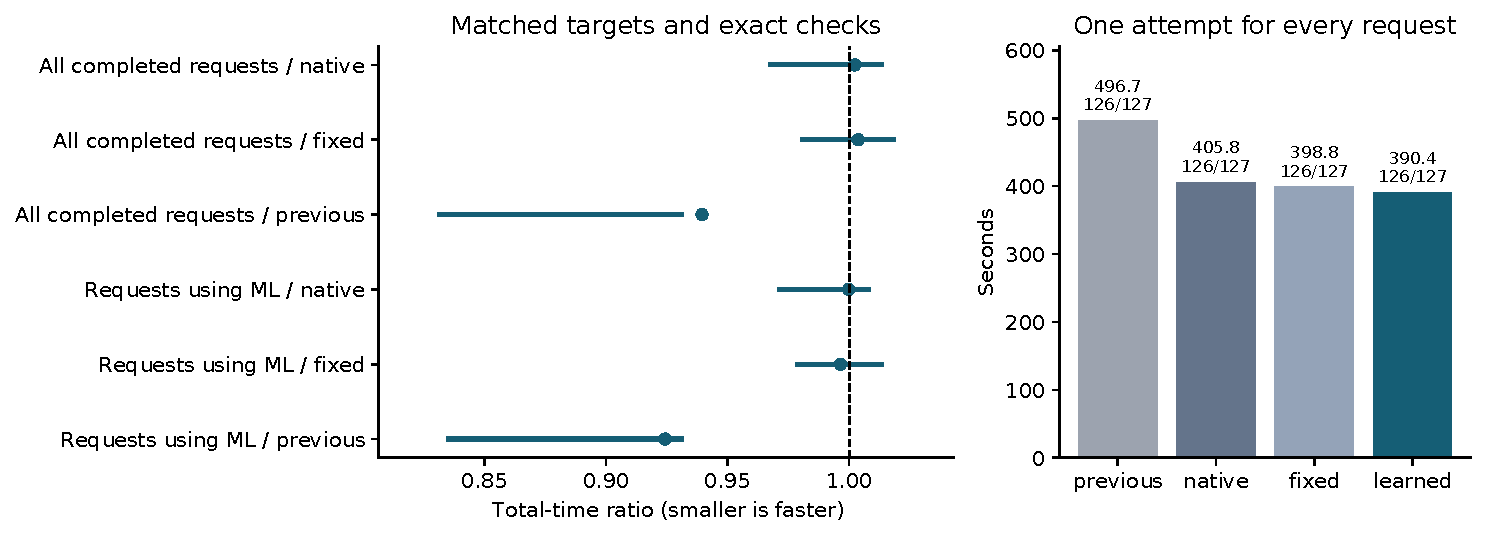
\includegraphics[width=\linewidth]{paper_figures/total_time_selection.pdf}
\caption{The left panel separates the complete application change from the added learned choice. Each point uses completed matched requests; bars show variation from resampling the three repetitions, and the dashed line marks equal time. The right panel includes one attempt for every requested calculation. Its labels give elapsed seconds and verified coverage, so an unfinished request cannot appear as a successful speedup.}
\label{fig:total-time}
\end{figure}
\begin{table}[!htbp]\centering\small
\caption{Use of the selector in each physical domain. The pentagon row is a subset of coupled requests. The ratio uses only matched requests that invoke the model, with the best fixed candidate as control. A dash means that no such comparison exists.}
\label{tab:total-domains}
\begin{tabularx}{\linewidth}{@{}Yrrrr@{}}\toprule
Domain & Requested & Verified & Use ML & ML/fixed\\\midrule
Coupled families & 49 & 48 & 31 & 0.988\\
Independent products & 52 & 52 & 51 & 0.999\\
Analytic formulas & 26 & 26 & 0 & --\\
Pentagon subset & 4 & 4 & 0 & --\\
\bottomrule\end{tabularx}\end{table}

Across every timed attempt, the learned application uses 1031.206 seconds, native choices use 1042.751, the fixed choice uses 1037.630, and the previous application uses 1207.572. These totals include all recorded repetitions and failures. Independent reference preparation takes 515.774 seconds outside the application timers. The existing checked master-basis preparation and training-label collection also precede deployment. The 497 training and validation action measurements use 1057.612 seconds in total, before independent reference preparation and 5.667 seconds of model fitting. The supplied-basis comparison therefore measures subsequent reductions, rather than a complete first-use calculation with unknown masters.

The high-loop results remain specific to the defined analytic families and products of small independent blocks. The coupled native tests reach three loops. No result establishes a globally minimum reduction time or complete coverage of arbitrary thirteen-loop scattering. The earlier seed and equation models retain their separate measured domains; the present selector keeps native equation and row choices, and we do not multiply savings from separate experiments.

\section{Derivation of the complete-time training rule}
\label{app:total-time}
For a target batch $i$ and an initial Kira setting $a$, let $T_{ia}$ be the measured time from application launch to exact comparison and process completion. This includes loading, selection, equation generation, algebra, and every recovery attempt. We define the training cost
\begin{equation}
 \begin{aligned}
 \widetilde T_{ia}^{(q)}&=\begin{cases}T_{ia}^{(q)},&\text{verified},\\
 \max(220\,\mathrm{s},T_{ia}^{(q)}),&\text{unverified},
 \end{cases}\\
 C_{ia}&=\operatorname{median}_{q}\widetilde T_{ia}^{(q)}.
 \end{aligned}
 \label{eq:total-cost}
\end{equation}
Here $q$ labels repetitions. The 220-second penalty is a training choice that makes an unfinished calculation costly; it does not estimate its unknown completion time. The results use measured seconds and completion counts, with no penalty substituted into reported speedups.

We construct a tree from structural features of the target integrals and their required master basis. In a leaf containing training requests $S$, choosing one action $a$ incurs total cost $\sum_{i\in S}C_{ia}$. Minimizing this expression gives the leaf action and cost,
\begin{equation}
 a_S=\arg\min_a\sum_{i\in S}C_{ia},\qquad
 J(S)=\min_a\sum_{i\in S}C_{ia}.
 \label{eq:total-leaf}
\end{equation}
A candidate feature threshold divides $S$ into disjoint sets $S_-$ and $S_+$. The two leaves can choose their actions separately, so their minimum combined cost is $J(S_-)+J(S_+)$. We therefore choose the threshold that gives the largest positive decrease
\begin{equation}
 \Delta J=J(S)-J(S_-)-J(S_+).
 \label{eq:total-split}
\end{equation}
This derivation trains the partition directly from elapsed reduction cost. Cost-sensitive algorithm selection also uses unequal penalties for expensive choices~\cite{Xu2011HydraMIP}. Our particular split rule follows from Eqs.~\eqref{eq:total-leaf}--\eqref{eq:total-split}; it does not certify a globally optimal tree or reduction path.

Each leaf stores the mean cost for every candidate action. A single tree predicts these means, while a forest averages the means from its reached leaves. If $\widehat C_a$ is the predicted cost, $a_0$ is the validation-selected anchor, $\delta$ is a decision margin, and $\tau=0.002\,\mathrm{s}$ is the decision allowance, the candidate $a_*=\arg\min_a\widehat C_a$ replaces the anchor only when
\begin{equation}
 \widehat C_{a_*}+\tau<(1-\delta)\widehat C_{a_0}.
 \label{eq:total-gate}
\end{equation}
The condition requires the predicted saving to exceed the allowance and margin. Validation must also show at least 1.5\% less cost than the best fixed candidate, with no increase in unverified requests, before the application enables learned decisions. Inputs outside the recorded structural ranges use native settings. These tests control deployment; they do not guarantee a saving on a new input.

The master-basis check also informs the seed region. For an integral with indices $\boldsymbol a$, define $r(\boldsymbol a)=\sum_j\max(a_j,0)$, $s(\boldsymbol a)=\sum_j\max(-a_j,0)$, $u(\boldsymbol a)=\sum_j\max(a_j-1,0)$, and $t(\boldsymbol a)=\sum_j\mathbf1_{a_j>0}$. These are the positive-power sum, numerator rank, number of dots, and number of positive indices. For the six basis-compatible candidates, we enlarge the corresponding bounds to contain the supplied basis. The unadjusted native candidate retains its original bounds. Kira's additional subsector restriction is $s\leq\max(1,t-\ell+1,s_{\mathrm{set}})$, where $s_{\mathrm{set}}$ is the explicitly assigned sector limit~\cite{Kira3}. Our first selector uses the stronger sufficient condition
\begin{equation}
 \ell\leq\min_{M}\{t(M)-s(M)\}.
 \label{eq:total-basis}
\end{equation}
We lower a proposed cutoff when needed to satisfy Eq.~\eqref{eq:total-basis}. It gives $t(M)-\ell+1\geq s(M)+1$, so each master passes the extra cutoff once the outer bounds contain it. This conservative choice can admit more seeds than necessary. It does not prove that the resulting identities suffice, so the application retains the exact master-basis check and less restrictive recovery settings.

\subsection{Target batches and basis features}
\label{app:total-targets}
The denominator definitions and rational kinematic profiles follow Appendix~\ref{app:families-new}. We specify the new target powers here so that the training and test batches have an explicit mathematical definition. Let $n$ be the number of physical denominators, let $N$ include the auxiliary coordinates, and define $b_j=1$ for $j\leq n$ and $b_j=0$ otherwise. For profile integer $h$ and target number $q=0,\ldots,\min(n,3)-1$, set
\begin{equation}
 i_q=1+((h+q)\bmod n),\qquad
 k_q=n+1+((h+q)\bmod(N-n)),\qquad
 v_q=1+(i_q\bmod n).
\end{equation}
The index $k_q$ is used only when $N>n$. With $\boldsymbol e_j$ denoting unit vector $j$, the four target shapes are
\begin{align}
 \boldsymbol a_q^{\rm dots}&=\boldsymbol b+(1+\mathbf1_{q=1})\boldsymbol e_{i_q},\\
 \boldsymbol a_q^{\rm mixed}&=\boldsymbol b+\boldsymbol e_{i_q}-\boldsymbol e_{k_q},\\
 \boldsymbol a_q^{\rm rank2}&=\boldsymbol b-2\boldsymbol e_{k_q},\\
 \boldsymbol a_q^{\rm pinched}&=\boldsymbol b-\boldsymbol e_{i_q}+\boldsymbol e_{v_q}.
\end{align}
Here $\mathbf1_{q=1}$ equals one for $q=1$ and zero otherwise. If there is no auxiliary coordinate, the mixed shape omits its numerator term and the rank-two shape becomes $\boldsymbol b+2\boldsymbol e_{i_q}$. The pinched shape removes one physical denominator and increases the next power by one. Training uses the first three shapes, validation uses the first two, and testing uses all four. We remove requests already handled by the exact formulas when defining the native training and validation collection. The pentagon structure is also excluded from both sets.

Independent products use the dotted shape for each vacuum, massive two-point, or ladder block. Their nonplanar box blocks and one-loop box remainders instead use $\boldsymbol b+2\boldsymbol e_{i_q}$ for each target. Blocks share external invariants and have disjoint loop momenta; cross-block auxiliary indices remain zero. At even loop order, the separate analytic test uses $\boldsymbol b+\boldsymbol e_{i_q}-\boldsymbol e_{k_q}$ when an auxiliary coordinate exists, and omits the numerator otherwise. At odd loop order it uses $\boldsymbol b+2\boldsymbol e_{i_q}$. The notes give the disjoint profile integers and preserve every resulting index vector in the measurement records.

For a nonempty master basis $\mathcal B$, define $r_B=\max_{M\in\mathcal B}r(M)$, $s_B=\max_{M\in\mathcal B}s(M)$, $u_B=\max_{M\in\mathcal B}u(M)$, and $\ell_B=\min_{M\in\mathcal B}[t(M)-s(M)]$. Let $s_T$ and $u_T$ be the corresponding target maxima, and write $x_+=\max(x,0)$. The seven added features are
\begin{equation}
 \boldsymbol z_B=(|\mathcal B|,r_B,s_B,u_B,\ell_B,
 (s_B-s_T)_+,(u_B-u_T)_+).
\end{equation}
These quantities describe the required basis before reduction. They contain no coefficient values. The implementation uses zeros for the basis summaries when the list is empty and applies no basis-dependent enlargement in that case.

\subsection{The seven candidate settings}
Let $r_T,s_T,u_T$ be target maxima and let $t_{\rm top}$ be the largest positive-index count among the declared top sectors. The unadjusted native candidate uses $(\max(t_{\rm top},r_T),s_T,u_T)$ and no subsector truncation. For an adjusted candidate with offsets $(\Delta r,\Delta s,\Delta u)$, the bounds are
\begin{equation}
 (r,s,u)=\bigl(\max(t_{\rm top},r_T+\Delta r,r_B),
 \max(s_T+\Delta s,s_B),\max(u_T+\Delta u,u_B)\bigr).
\end{equation}
Table~\ref{tab:total-actions} completes the action definition. A dash disables the extra subsector cutoff. The native region, raised rank, and expanded region provide recovery choices when a restricted region fails its exact basis check.
\begin{table}[!htbp]\centering\small
\caption{The six basis-compatible candidates, in addition to the unadjusted native candidate.}
\label{tab:total-actions}
\begin{tabularx}{\linewidth}{@{}Ycl@{}}\toprule
Candidate & $(\Delta r,\Delta s,\Delta u)$ & Subsector cutoff $\ell$\\\midrule
Compatible native & $(0,0,0)$ & --\\
Increased rank & $(0,1,0)$ & --\\
Enlarged region & $(1,1,1)$ & --\\
Truncated & $(0,0,0)$ & $\min(t_{\rm top}-s_T,\ell_B)$\\
Truncated with increased rank & $(0,1,0)$ & $\min(t_{\rm top}-s_T,\ell_B)$\\
Relaxed truncation & $(0,0,0)$ & $\min(t_{\rm top}-s_T-1,\ell_B)$\\\bottomrule
\end{tabularx}
\end{table}

\section{Details of complete-time selection}
\label{app:total-time-details}
The training parameter profile is 1901 and the validation profile is 1907. Training targets use dots, a dot with one numerator power, and numerator rank two; exact formulas remove some requests before native collection. Validation uses the first two shapes. Reserved native requests use profile 2011 and additionally include pinched targets; products use $2027+4L$, analytic requests use 2039, and the three-loop ladder uses 2053. No reserved measurement changes the trained selector. We collected the unadjusted native-bound candidate after the six adjusted candidates, before model fitting. The reserved comparison then times all four methods in rotated order on the same worker for each request.

The candidates use seven seed settings, thirty tree or forest structures, two possible anchor settings where distinct, and margins $0$, $0.03$, $0.08$, or $0.15$. A forest draws sixteen bootstrap samples, each the size of the training collection, and samples fourteen features at each node. Leaves store mean complete costs. A single tree examines all features. Threshold searches use at most seventeen feature values. The split must save more than $0.002$ seconds per request in its training node. The feature-range guard checks loop and external-momentum counts, index counts, symbolic-invariant counts, maximum dots and rank, positive-index counts, massive and coupled denominators, loop incidence and degree, maximum positive-power sum, target-sector deficit, and the basis dot gap.

Validation chooses d2\_n4\_t16\_a0\_m0.0. Model fitting takes 5.667 seconds; the timed collection of native training labels is a separate cost. The deployment flag is enabled. The table below preserves coverage at every loop order.
\begin{center}\small
\begin{tabular}{@{}rrrrr@{}}\toprule
Loops & Requested & Learned verified & Native verified & Fixed verified\\\midrule
1 & 23 & 23 & 23 & 23\\
2 & 29 & 29 & 29 & 29\\
3 & 15 & 14 & 14 & 14\\
4 & 6 & 6 & 6 & 6\\
5 & 6 & 6 & 6 & 6\\
6 & 6 & 6 & 6 & 6\\
7 & 6 & 6 & 6 & 6\\
8 & 6 & 6 & 6 & 6\\
9 & 6 & 6 & 6 & 6\\
10 & 6 & 6 & 6 & 6\\
11 & 6 & 6 & 6 & 6\\
12 & 6 & 6 & 6 & 6\\
13 & 6 & 6 & 6 & 6\\
\bottomrule\end{tabular}\end{center}

% END CURRENT WORKFLOW UPDATE
% BEGIN CURRENT WORKFLOW UPDATE
% REFINED TIME SELECTION
\section{Selecting the method by complete reduction time}
\label{sec:refined-time}
The target integrals and required master basis determine which seed regions can support a reduction. A region that excludes a required master can cause an unsuccessful attempt and a repeat calculation. We therefore include basis information in both the model inputs and the candidate settings, and train the model to minimize the complete time after recovery. Kira's subsector cutoff admits numerator ranks zero and one, and can also admit a master through an explicitly assigned sector limit~\cite{Kira3}. Two candidates use this condition to retain the required masters with the least enlargement of that cutoff. The selector compares their measured cost with seven other settings. Exact formulas and independent-loop factorization precede prediction, and Kira computes the coefficients for each remaining native block.

\subsection{Training and integration}
The nine settings include the original native bounds, six conservative basis-compatible candidates, and two candidates with the tighter cutoff condition. The new pair uses the ordinary or increased numerator-rank bound. Appendix~\ref{app:refined-time} derives the new condition from Kira's cutoff, while Appendix~\ref{app:total-time} gives the shared timing objective and structural inputs. Every candidate retains the exact basis check and recovery code. The exact formulas retain their assumptions from Appendix~\ref{app:blocks13}.

The model receives the 44 structural inputs used above and seven summaries of the supplied master basis. These additional inputs describe its size, positive-power bounds, numerator ranks, dots, truncation limit, and differences from the target bounds. No family name or parameter-profile identifier enters the features. Each candidate action is timed through process completion and an independent exact coefficient check, including failed attempts and recovery. We use one repetition for each training action and two for each validation action. Unverified outcomes receive a declared training penalty and remain in the evidence.

The collection contains 31 training requests and 20 validation requests, with separate rational parameter profiles and symbolic dimension. It covers vacuum, two-point, and scattering structures through three loops. Pentagon requests are absent from both sets. We fit trees with maximum depths one through five and minimum leaf sizes two, four, or seven, using either one tree or sixteen trees. The split objective minimizes elapsed reduction cost. Validation retains the fixed setting because the fitted candidates do not meet the declared improvement threshold. The deployed application therefore performs no tree prediction. It compares the selected method with the fastest fixed candidate before enabling prediction. The selected fixed action is a truncation with the tighter basis condition and increased rank. The validation totals are 42.586 seconds for the selected application, 45.714 for native choices, and 42.586 for the fixed candidate. The model changes the best fixed action on 0 of the 20 validation requests. These are model-selection measurements.

The application loads model weights and computes predictions only for a block that needs native algebra. An exact formula therefore incurs no model prediction. Identical independent blocks share one reduction within the request, and the resulting product remains factored. When prediction is enabled, a structural-range check sends inputs outside the training ranges to native settings. The selector also retains native settings when no checked master basis is available. These rules avoid unsupported learned choices; they do not establish that an unseen integral will reduce quickly.

\subsection{Reserved comparison}
We freeze the weights and decision rules before using the new test profiles. Every request compares the learned application, native choices, a validation-selected fixed choice, and the previously published application. The first three methods use identical exact formulas, basis checks, and recovery code. The native control uses the original seed bounds; the learned and fixed methods choose from the same nine candidates. The comparison with the best fixed choice therefore measures the added request-dependent decision. The previous application also differs in basis-aware seeding, model implementation, and output handling, so that comparison measures the complete update.

The test contains 65 requests. It includes new target shapes and parameter values, the held-out pentagon structure, independent products through thirteen loops, the two specified analytic families at thirteen loops, and the previously difficult three-loop ladder. Each method runs three times in rotated order on the same worker. A method that fails its first exact check receives no further repetitions for that request. The learned application completes all three checks on 64 requests; Table~\ref{tab:refined-time} retains the other outcomes.

On 64 matched requests, the application uses 209.217 seconds against 228.710 seconds for the previous application, or 8.5\% less time. The time ratio is 0.915, with repetition interval $[0.864,0.918]$. On 64 matched requests, the application uses 209.217 seconds against 213.807 seconds for native bounds, or 2.1\% less time. The time ratio is 0.979, with repetition interval $[0.962,0.990]$. On 64 matched requests, the application uses 209.217 seconds against 210.378 seconds for the best fixed setting, or 0.6\% less time. The time ratio is 0.994, with repetition interval $[0.984,1.008]$. Validation leaves prediction off. These measurements describe the fixed workflow and do not establish an added gain from the fitted forest.

\begin{table}[!htbp]\centering\small
\caption{Complete-time comparison on the same requested workload. The first-pass column includes one timed attempt for every request, including unverified outcomes. Each ratio divides the summed request medians for the learned method by those for the listed method, using only their matched exact completions.}
\label{tab:refined-time}
\begin{tabular}{@{}lrrrr@{}}\toprule
Method & Verified requests & First pass (s) & Learned/method & Failed calls\\\midrule
Previous application & 64/65 & 343.848 & 0.915 & 36\\
Native choices & 64/65 & 286.701 & 0.979 & 5\\
Fixed choice & 64/65 & 283.179 & 0.994 & 2\\
Learned selector & 64/65 & 280.860 & 1.000 & 2\\
\bottomrule\end{tabular}
\end{table}
\begin{figure}[!htbp]\centering
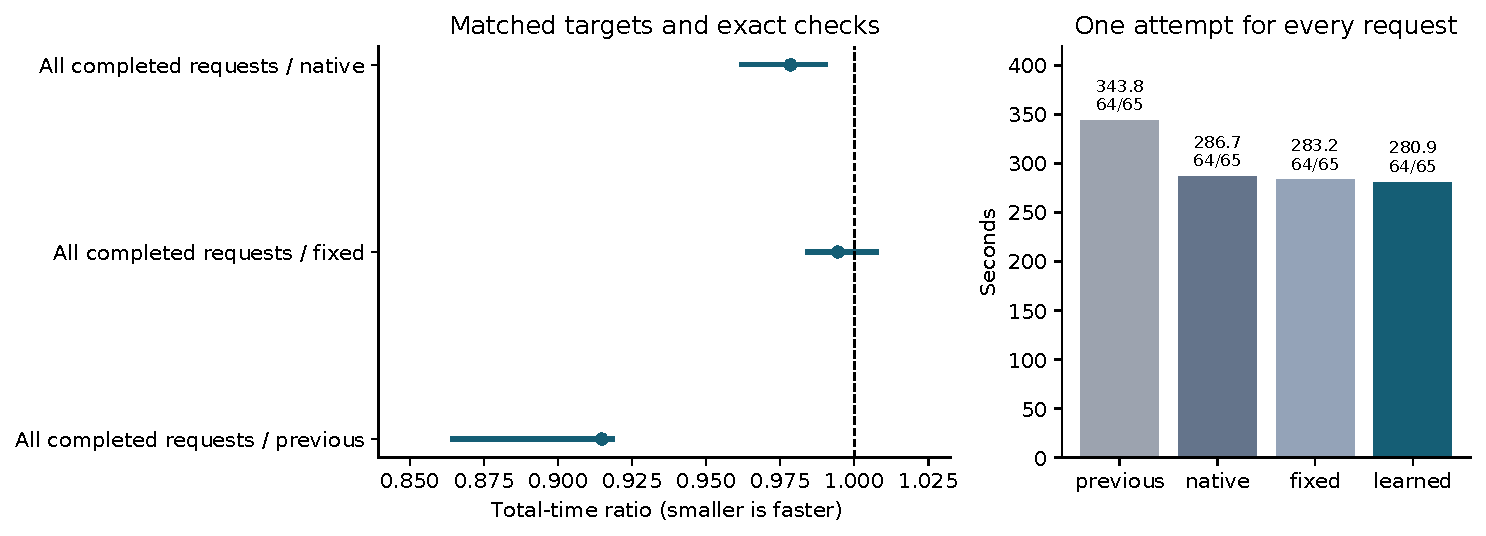
\includegraphics[width=\linewidth]{paper_figures/refined_time_selection.pdf}
\caption{The left panel separates the complete application change from the added learned choice. Each point uses completed matched requests; bars show variation from resampling the three repetitions, and the dashed line marks equal time. The right panel includes one attempt for every requested calculation. Its labels give elapsed seconds and verified coverage, so an unfinished request cannot appear as a successful speedup.}
\label{fig:refined-time}
\end{figure}
\begin{table}[!htbp]\centering\small
\caption{Use of the selector in each physical domain. The pentagon row is a subset of coupled requests. The ratio uses only matched requests that invoke the model, with the best fixed candidate as control. A dash means that no such comparison exists.}
\label{tab:refined-domains}
\begin{tabularx}{\linewidth}{@{}Yrrrr@{}}\toprule
Domain & Requested & Verified & Use ML & ML/fixed\\\midrule
Coupled families & 29 & 28 & 0 & --\\
Independent products & 34 & 34 & 0 & --\\
Analytic formulas & 2 & 2 & 0 & --\\
Pentagon subset & 2 & 2 & 0 & --\\
\bottomrule\end{tabularx}\end{table}

Across every timed attempt, the learned application uses 701.490 seconds, native choices use 715.190, the fixed choice uses 703.361, and the previous application uses 814.261. These totals include all recorded repetitions and failures. Independent reference preparation takes 440.803 seconds outside the application timers. The existing checked master-basis preparation and training-label collection also precede deployment. The 639 training and validation action measurements use 1509.683 seconds in total, before independent reference preparation and 8.568 seconds of model fitting. The supplied-basis comparison therefore measures subsequent reductions, rather than a complete first-use calculation with unknown masters.

The high-loop results remain specific to the defined analytic families and products of small independent blocks. The coupled native tests reach three loops. No result establishes a globally minimum reduction time or complete coverage of arbitrary thirteen-loop scattering. The earlier seed and equation models retain their separate measured domains; the present selector keeps native equation and row choices, and we do not multiply savings from separate experiments.

\section{A tighter condition for the master-basis cutoff}
\label{app:refined-time}
The cost objective, target definitions, and 51 inputs remain those in Appendix~\ref{app:total-time}. The new model learns from fresh profiles, and all nine candidate costs for one request are measured together on the same worker. The notes give the training and test profiles and the selected model parameters.

Kira restricts the numerator rank in a sector through~\cite{Kira3}
\begin{equation}
 s\leq\max\{1,t-\ell+1,s_{\mathrm{set}}\}.
 \label{eq:refined-cutoff}
\end{equation}
Here $t$ is the sector's positive-index count, $\ell$ is the truncation parameter, and $s_{\mathrm{set}}$ is the rank limit explicitly assigned to that sector. A master with rank $s_M\leq\max(1,s_{\mathrm{set},M})$ already satisfies this additional cutoff for any $\ell$. For every other master, Eq.~\eqref{eq:refined-cutoff} reduces to $s_M\leq t_M-\ell+1$. Rearranging gives $\ell\leq t_M+1-s_M$.

Let $\mathcal H$ contain precisely the masters with $s_M>\max(1,s_{\mathrm{set},M})$. If $\ell_0=t_{\mathrm{top}}-s_T$ is the proposed truncation value, the largest value no greater than $\ell_0$ that admits all required masters is therefore
\begin{equation}
 \ell_* = \min\left(\ell_0,\min_{M\in\mathcal H}\{t_M+1-s_M\}\right).
 \label{eq:refined-basis}
\end{equation}
An empty inner set imposes no bound, so $\ell_*=\ell_0$ in that case. Taking the minimum enforces each master's inequality, while any larger value would violate at least one of the active bounds or exceed the proposed value. Thus Eq.~\eqref{eq:refined-basis} is the least enlargement needed for this particular cutoff-admission condition. It does not determine a sufficient IBP system or a minimum reduction time.

The two added candidates use $\ell_*$ with the ordinary or increased numerator-rank bound. Their outer positive-power, numerator-rank, and dot bounds still contain the supplied master basis. The explicitly seeded top sectors use the candidate's assigned rank bound; other sectors have $s_{\mathrm{set}}=0$ unless explicitly declared. The previous seven candidates remain available, so the trained policy can select a conservative setting when its complete cost is lower. Every candidate keeps the exact coefficient and master-basis checks, and failed attempts retain their recovery cost in training and testing.

\section{Details of complete-time selection}
\label{app:refined-time-details}
The training parameter profile is 2101 and the validation profile is 2107. Training targets use dots, a dot with one numerator power, and numerator rank two; exact formulas remove some requests before native collection. Validation uses the first two shapes. Reserved native requests use profile 2203, with rank-two and pinched targets added for three structures; products use $2213+4L$, the thirteen-loop analytic requests use 2221, and the three-loop ladder uses 2227. The product grid includes all four structures at odd loop orders and one rotating structure at each even order. No reserved measurement changes the trained selector. We time all nine training candidates together in rotated order on the same worker for each request. The reserved comparison also uses rotated method order.

The candidates use nine seed settings, thirty tree or forest structures, two possible anchor settings where distinct, and margins $0$, $0.03$, $0.08$, or $0.15$. A forest draws sixteen bootstrap samples, each the size of the training collection, and samples fourteen features at each node. Leaves store mean complete costs. A single tree examines all features. Threshold searches use at most seventeen feature values. The split must save more than $0.002$ seconds per request in its training node. The feature-range guard checks loop and external-momentum counts, index counts, symbolic-invariant counts, maximum dots and rank, positive-index counts, massive and coupled denominators, loop incidence and degree, maximum positive-power sum, target-sector deficit, and the basis dot gap.

Validation chooses d3\_n2\_t16\_a0\_m0.0. Model fitting takes 8.568 seconds; the timed collection of native training labels is a separate cost. The deployment flag is disabled. The table below preserves coverage at every loop order.
\begin{center}\small
\begin{tabular}{@{}rrrrr@{}}\toprule
Loops & Requested & Learned verified & Native verified & Fixed verified\\\midrule
1 & 12 & 12 & 12 & 12\\
2 & 17 & 17 & 17 & 17\\
3 & 9 & 8 & 8 & 8\\
4 & 1 & 1 & 1 & 1\\
5 & 4 & 4 & 4 & 4\\
6 & 1 & 1 & 1 & 1\\
7 & 4 & 4 & 4 & 4\\
8 & 1 & 1 & 1 & 1\\
9 & 4 & 4 & 4 & 4\\
10 & 1 & 1 & 1 & 1\\
11 & 4 & 4 & 4 & 4\\
12 & 1 & 1 & 1 & 1\\
13 & 6 & 6 & 6 & 6\\
\bottomrule\end{tabular}\end{center}

% END CURRENT WORKFLOW UPDATE
% BEGIN CURRENT WORKFLOW UPDATE
% HYBRID EXPERT COMPARISON
\section{Combining learned and exact reduction methods}
\label{sec:hybrid-experts}
The complete-time comparison above retains a fixed setting for the broad request collection. The earlier sparse-seed model has a separate tested use for nonplanar two-loop integrals with higher numerator powers. We therefore combine these methods and measure their complete costs on fresh inputs. Exact formulas handle their supported families first, and independent loop blocks are reduced separately. For the remaining work, the application can use the preceding setting, a fixed sparse boundary, the trained sparse-seed expert, or the original native bounds. Every route retains exact Kira algebra, the supplied master-basis check, and recovery after an unsuccessful attempt.

\subsection{The sparse expert and the complete-time selector}
The sparse expert acts before Kira generates equations. It uses the target numerator powers to select the boundary of a seed region, as defined in Appendix~\ref{app:seed-geometry}. Its validated input domain contains one target in the specified nonplanar massless two-loop box, with seven unit physical powers and numerator rank two, three, or four. We check the ordered denominator and momentum structure before using this expert. Other blocks use the preceding fixed setting within its training ranges and return to original native bounds outside those ranges. The range check also covers numerator ranks above the broad training collection. This domain restriction permits a useful local model without assigning it an unsupported task.

The expert retains its previously trained 32-tree model with maximum depth 2. Its 12 original training requests and 10 model-selection requests precede this experiment. The model predicts log-time ratios for candidate sparse boundaries from 68 inputs: 27 family and target summaries, 40 positive- and negative-power coordinates, and the largest number of negative entries. Tree evaluation uses the saved thresholds and mean leaf values, following the earlier extremely randomized forest construction~\cite{Geurts2006ExtraTrees}. Appendix~\ref{app:hybrid-experts} gives the candidate boundaries and the fresh target batches. The current comparison includes feature calculation, prediction, seed enumeration, input preparation, and every recovery attempt.

We then fit an outer cost model from new complete reduction times. It receives the 51 structural and master-basis inputs of Appendix~\ref{app:total-time}, together with the two auxiliary numerator powers for this ordered family. Its four actions are the four routes listed above. The training cost includes the inner expert's prediction when that route uses it. We use the direct cost split of Eq.~\eqref{eq:total-split}, so the outer model learns which complete route takes less time.

The new collection has 16 training requests and 8 validation requests with separate rational kinematics. Each training action is measured once and each validation action twice. We compare one tree or sixteen trees, maximum depths one through five, and minimum leaf sizes two, four, or seven. Validation first compares the outer prediction with the best constant route. It then compares the resulting application with the best ML-free candidate. Each deployment comparison requires at least 1.5\% less validation cost and no increase in unverified requests. The fixed sparse candidate retains the boundary selected in the earlier expert study. Current validation compares that candidate with the preceding setting and original native bounds to select the ML-free control. The selected control is a fixed sparse-seed boundary. Validation enables the outer 1-tree model, with maximum depth 2 and minimum leaf size 4. The selected validation cost is 52.826 seconds, compared with 55.917 seconds for the ML-free control. These model-selection results precede the reserved test.

\subsection{Fresh complete-workflow comparison}
The reserved comparison contains twenty-four nonplanar target requests and ten compatibility requests. The nonplanar requests cover every distribution of numerator ranks two through four across the two auxiliary coordinates at two new kinematic profiles. Eight of these requests use index vectors absent from the new outer-model training and validation collection. The earlier inner expert has a separate training history, which includes some of these added shapes. The ten compatibility requests include native coupled families through three loops, independent products through thirteen loops, and a thirteen-loop analytic case. We freeze the expert weights, outer model, domain checks, and decisions before testing. Each request uses three repetitions with rotated method order on one worker. The preceding application runs through its actual entry point. The fixed control disables both learned predictions, while all routes retain exact coefficient checks and the same native resource limits.

The integrated application verifies 34 of 34 requests in all three repetitions, and invokes learned prediction on 24. For 34 matched requests, the integrated method takes 156.290 seconds and the preceding complete-time application takes 161.592 seconds. This gives 3.3\% less time, with ratio 0.967 and repetition interval $[0.950,1.003]$. For 24 matched requests, the integrated method takes 136.956 seconds and native seed bounds takes 225.338 seconds. This gives 39.2\% less time, with ratio 0.608 and repetition interval $[0.584,0.640]$. For 24 matched requests, the integrated method takes 136.956 seconds and the validation-selected ML-free control takes 143.079 seconds. This gives 4.3\% less time, with ratio 0.957 and repetition interval $[0.925,0.998]$. The comparison with the selected ML-free control resolves an added saving from learned decisions beyond the measured repetition variation. For 8 matched requests, the integrated method takes 52.876 seconds and the validation-selected ML-free control takes 51.685 seconds. This gives 2.3\% more time, with ratio 1.023 and repetition interval $[0.974,1.109]$. For 8 matched requests, the integrated method takes 52.876 seconds and the preceding complete-time application takes 48.131 seconds. This gives 9.9\% more time, with ratio 1.099 and repetition interval $[1.066,1.194]$. These added index patterns expose a remaining transfer limit for the outer selector.

\begin{table}[!htbp]\centering\small
\caption{Complete hybrid comparison. The first-pass time includes one attempt at every requested calculation. Ratios use sums of request medians on matched exact completions. The fixed setting is selected from the three declared ML-free candidates on validation data.}
\label{tab:hybrid-experts}
\begin{tabular}{@{}lrrrr@{}}\toprule
Method & Verified & First pass (s) & Integrated/method & Failed calls\\\midrule
Preceding application & 34/34 & 162.721 & 0.967 & 0\\
Native bounds & 34/34 & 243.584 & 0.636 & 0\\
Selected ML-free control & 34/34 & 165.651 & 0.961 & 48\\
Integrated method & 34/34 & 159.543 & 1.000 & 0\\
\bottomrule\end{tabular}\end{table}
\begin{figure}[!htbp]\centering
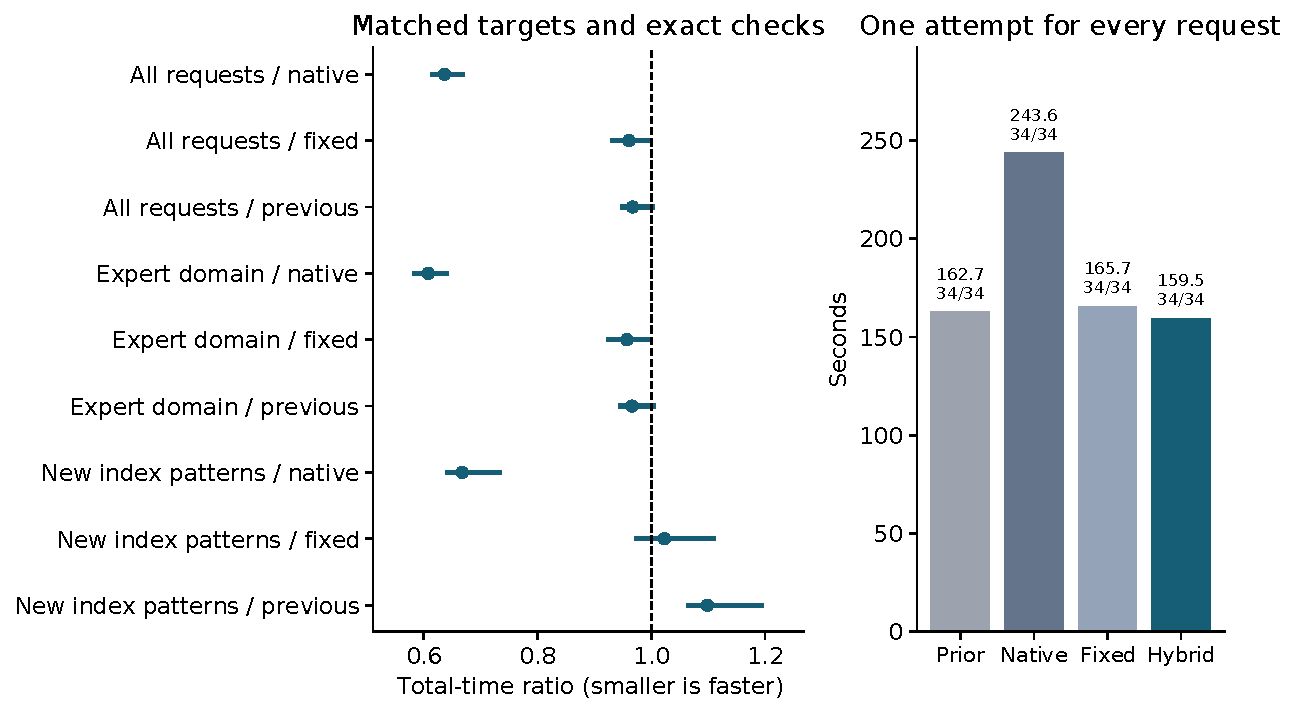
\includegraphics[width=\linewidth]{paper_figures/hybrid_expert_selection.pdf}
\caption{The left panel gives complete-time ratios for all matched requests, the sparse-expert domain, and the additional index patterns absent from outer-model training. The fixed control isolates the added learned decision. The line at one marks equal time, and horizontal bars show paired repetition variation. The right panel includes one attempt for every request and labels verified coverage. Prior and Hybrid denote the preceding and integrated applications.}
\label{fig:hybrid-experts}
\end{figure}
Across all recorded attempts and repetitions, the integrated method takes 476.353 seconds, compared with 493.287 seconds for the ML-free setting and 487.815 seconds for the preceding application. The 128 new training and validation measurements take 1033.449 timed seconds; outer-model fitting takes 12.241 seconds. Independent reference preparation for the reserved requests takes 908.971 seconds outside the application timers. The earlier expert training and checked master-basis preparation are additional prior costs.

The comparison measures use with an existing checked basis and includes model loading, prediction, equation generation, algebra, exact checks, and recovery. The direct learned result applies to the specified nonplanar family and numerator range. The compatibility checks verify the retained routes on their stated families; the broader baseline comparison above remains a separate experiment. The application keeps native row and equation choices. These finite tests establish no globally fastest reduction or coverage of arbitrary high-loop scattering.

\section{Definition of the hybrid expert comparison}
\label{app:hybrid-experts}
The sparse expert uses the nonplanar denominators in Eq.~\eqref{eq:nonplanar-new}. Its targets have seven unit physical powers. For numerator rank $R=2,3,4$, we include
\begin{equation}
 \boldsymbol a^{(1)}_R=(1,1,1,1,1,1,1,-R,0),\qquad
 \boldsymbol a^{(2)}_R=(1,1,1,1,1,1,1,0,-R).
\end{equation}
For $R=3,4$, we also include
\begin{equation}
 \boldsymbol a^{(12)}_R=(1,1,1,1,1,1,1,-\lceil R/2\rceil,-\lfloor R/2\rfloor).
\end{equation}
These definitions give eight training and validation targets per kinematic profile. The reserved collection additionally includes every vector $(1,1,1,1,1,1,1,-j,-(R-j))$ for $j=0,\ldots,R$ and $R=2,3,4$, giving twelve targets per profile. We use $s=-113-18h$ and $t=-127-10h$, with $h=2301,2303$ for training, $2309$ for validation, and $2311,2317$ for reserved tests. The additional two outer-model inputs are $\max(0,-a_8)$ and $\max(0,-a_9)$, appended to the 51 inputs in Appendix~\ref{app:total-time}. Their coordinate meanings remain fixed within this ordered family.

The outer actions are the preceding basis-compatible setting, the expert's fixed sparse boundary, its learned boundary, and original native bounds. The best ML-free control minimizes validation cost over all but the learned boundary. The cost-sensitive tree objective follows Eqs.~\eqref{eq:total-cost}--\eqref{eq:total-gate}, with complete costs for these four actions. The outer prediction is retained only if it improves on the best constant action by at least 1.5\%. The resulting application must also improve on the best ML-free candidate by at least 1.5\%, with no increase in unverified requests. A constant choice of the learned expert still performs that expert's target-dependent boundary prediction.

For the inner expert, the boundary coefficients $\theta_0,\ldots,\theta_6$ have the definitions in Appendix~\ref{app:seed-geometry}. The saved forest predicts log-time ratios for these candidates. It changes the fixed candidate only when the predicted decrease exceeds its frozen margin. Table~\ref{tab:hybrid-boundaries} records the candidate coefficients; the native row applies no sparse boundary. Target and master seeds that satisfy the outer native bounds remain explicitly included. The native master-basis and coefficient checks determine acceptance, and a failed sparse attempt returns to less restrictive native work.

\begin{table}[!htbp]\centering\small
\caption{Frozen sparse-boundary candidates used by the inner expert. Coefficients define the seed region of Eq.~\eqref{eq:geometry-boundaries}.}
\label{tab:hybrid-boundaries}
\begin{tabular}{@{}lrrrrrrr@{}}\toprule
Candidate & $\theta_0$ & $\theta_1$ & $\theta_2$ & $\theta_3$ & $\theta_4$ & $\theta_5$ & $\theta_6$\\\midrule
0: native & -- & -- & -- & -- & -- & -- & --\\
1 & 1 & 0 & 0 & 1 & 0 & 1 & 0\\
2 & 2 & 0 & 0 & 1 & 0 & 1 & 0\\
3 & 1 & 0 & 0 & 0 & 0 & 1 & 0\\
4 & 1 & 0 & 0 & 0 & 1 & 1 & 0\\
5 & 1 & 0 & 0 & -1 & 0 & 1 & 0\\
6 & 1 & 0 & 0 & 1 & 1.5 & 1 & 0\\
7 & 1.5 & -0.25 & 0 & 1.25 & 0 & 1 & -0.25\\
8 & 2 & 0 & -0.25 & 1 & 0 & 1 & 0\\
9 & 2.5 & 0 & 0 & 1.25 & 0 & 1 & -0.25\\
\bottomrule\end{tabular}\end{table}

The fixed boundary index is 4 and the inner decision margin is 0. The ten compatibility requests use profile 2321 for the three original coupled native families, a pentagon, a rank-three massive two-point target, and the one-mass analytic family, and profiles $2327+4L$ for four independent products. Their denominators and target rules remain those in Appendices~\ref{app:families-new} and~\ref{app:total-targets}. They provide checks at loop orders one, two, three, four, eight, twelve, and thirteen.

For the selected tree, let $u=\max(0,-a_8)$ be the first auxiliary numerator power and let $R=\max(0,-a_8)+\max(0,-a_9)$ be the total numerator rank. The first split tests $u\leq2.5$, and its lower branch tests $R\leq3.5$. Since both quantities are integers, the deployed choice within the expert domain is
\begin{equation}
 \pi(u,R)=\begin{cases}
  \text{learned sparse boundary},&u\leq2,\ R\leq3,\\
  \text{fixed sparse boundary},&u\leq2,\ R=4,\\
  \text{preceding basis-compatible setting},&u\geq3.
 \end{cases}
 \label{eq:hybrid-tree}
\end{equation}
Here $\pi(u,R)$ is the selected reduction route. Each leaf selects the route with its lowest predicted complete cost, subject to the decision allowance of Eq.~\eqref{eq:total-gate}. For the first two leaves, the predicted saving relative to the anchor exceeds the 0.002-second allowance. The third leaf already selects the anchor, so the allowance leaves its choice unchanged. These comparisons give Eq.~\eqref{eq:hybrid-tree}. Thus the outer tree can select a fixed or native setting even within the sparse expert's supported family. The exact checks and recovery rules still apply to each selected route.

% END CURRENT WORKFLOW UPDATE
% BEGIN CURRENT WORKFLOW UPDATE
\section{Combined decomposition with the analytic recurrence}
\label{sec:notes-analytic-results}
The initial analytic-enabled comparison measures the added recurrence while preserving the existing learned models. It contains 16 rational-kinematics polygon requests, two fully symbolic two-point requests, 12 independent bubble products covering loop orders two through thirteen, eight nonplanar two-loop requests, and three further compatibility requests. Appendix~\ref{app:notes-analytic-inputs} specifies the denominators, targets, and parameter choices. Each method starts in a fresh process, and three repetitions rotate the method order on the same worker.

All four methods use the same independent-block factorization and share identical blocks within a request. The native control receives the same prepared master indices and uses the existing exact block formulas, but it generates native IBP equations for the newly supported one-loop blocks. The exact fixed control uses the new recurrence and disables learned choices. The preceding application runs unchanged with its earlier master-index cache. Its timer includes discovery and a second check when that cache lacks a structure. The matched native control receives the new prepared indices, which separates the recurrence benefit from this cache extension. Thus the native comparison measures the combined analytic and learned change, while the exact fixed comparison isolates the current learned contribution.

\begin{table}[!htbp]\centering\small
\caption{Complete decomposition times, summed over per-request medians. Speedup is native-control time divided by combined time. The last column is combined time divided by exact fixed-control time. Ratios below one in that column favor learned selection. Only requests verified in all three repetitions enter a paired sum.}
\label{tab:notes-analytic-results}
\begin{tabular}{@{}lrrrrr@{}}\toprule
Collection & $N$ & Combined (s) & Native (s) & Speedup & ML/fixed\\\midrule
Scalar one-loop polygons & 18 & 14.815 & 20.862 & 1.41 & 0.991 \\
Independent products & 12 & 4.524 & 9.522 & 2.10 & 1.063 \\
Coupled ML cases & 8 & 43.037 & 71.455 & 1.66 & 0.936 \\
Other compatibility cases & 3 & 2.890 & 2.918 & 1.01 & 0.978 \\
All requests & 41 & 65.266 & 104.757 & 1.61 & 0.958 \\
\bottomrule\end{tabular}
\end{table}

The combined application completes 41 of 41 requests in all three repetitions. The native, exact fixed, and preceding applications complete 41, 41, and 41 requests, respectively. Including every requested first attempt, the combined application takes 68.401 seconds. Independent reference and master-index preparation takes 357.770 seconds and remains outside the supplied-basis timer.

Against the actual preceding application, the combined method takes 65.266 seconds, compared with 103.134 seconds on 41 matched requests, giving a speedup of 1.58. This comparison includes each application's own preparation and recovery inside its timer.

Across all repetitions, the combined application makes 30 native calls, compared with 120 for the matched native control. The exact fixed control makes 48 calls, including 18 unsuccessful attempts before recovery. The combined method has 0 failed native calls. Thus the recurrence removes native work in its domain, and the retained learned selector avoids the failed sparse attempts observed with the fixed choice.

For the requests that use the new recurrence, the combined application uses 36.4\% less time than the matched native control. The time ratio is 0.636, with repetition interval $[0.608,0.748]$.

For the requests that use the new recurrence, the combined application uses 0.7\% more time than the exact fixed control. The time ratio is 1.007, with repetition interval $[0.787,1.208]$. This interval includes equal times, so this comparison does not resolve a saving beyond the observed repetition variation.

For the coupled nonplanar requests, the combined application uses 39.8\% less time than the matched native control. The time ratio is 0.602, with repetition interval $[0.568,0.635]$.

For the coupled nonplanar requests, the combined application uses 6.4\% less time than the exact fixed control. The time ratio is 0.936, with repetition interval $[0.873,0.988]$.

For all matched requests, the combined application uses 37.7\% less time than the matched native control. The time ratio is 0.623, with repetition interval $[0.599,0.662]$.

For all matched requests, the combined application uses 4.2\% less time than the exact fixed control. The time ratio is 0.958, with repetition interval $[0.869,1.017]$. This interval includes equal times, so this comparison does not resolve a saving beyond the observed repetition variation.

\begin{figure}[!htbp]\centering
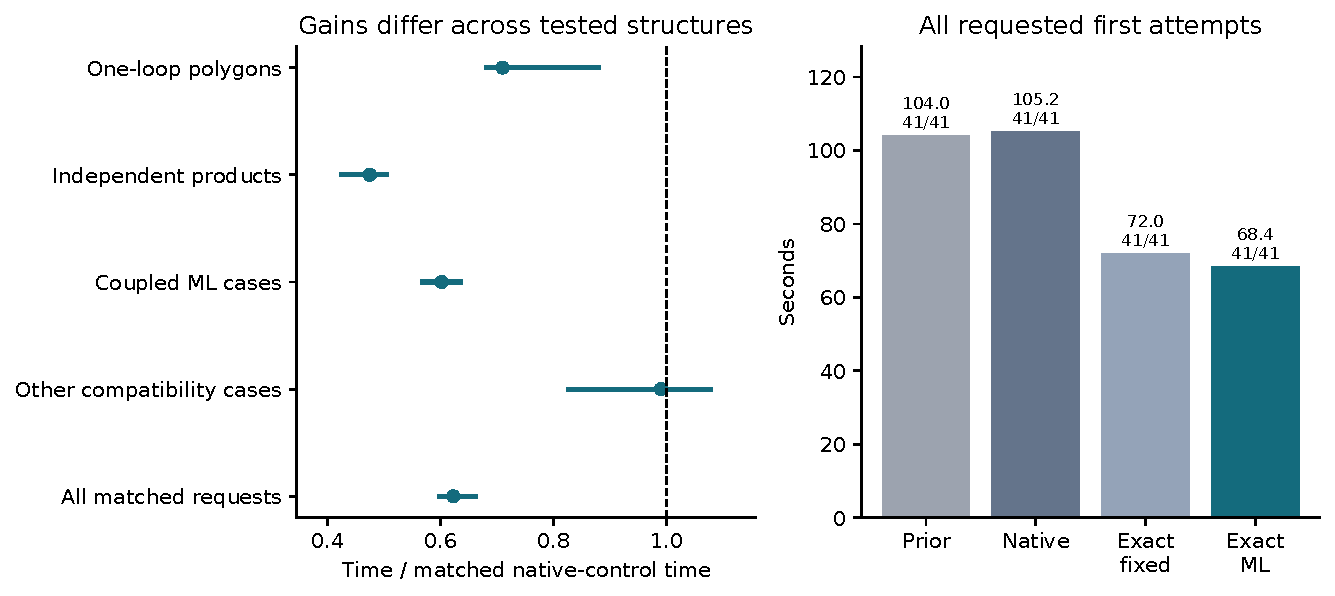
\includegraphics[width=\linewidth]{paper_figures/analytic_decomposition.pdf}
\caption{The left panel compares complete verified reductions with the matched native control. The right panel includes every first attempt and gives completed-request counts above the bars. Intervals describe resampling of three timing repetitions on these fixed requests; they do not establish transfer to every integral family.}
\label{fig:notes-analytic-decomposition}
\end{figure}

The analytic improvement comes from the derived recurrence and shared exact subproblems. The models retain their earlier weights and supported domain, so this experiment does not represent new model training. Independent products provide exact tests through thirteen loops, but their connected components remain one-loop integrals. The separate compatibility cases preserve connected native tests through three loops and the existing thirteen-loop vacuum formula. These measurements do not establish a general analytic solution or a universal speedup for connected high-loop scattering.

The two fully symbolic requests expose a cost hidden by the collection average: their analytic-enabled medians are 1.59 and 3.52 times the matched native medians. Each fresh process loads and uses symbolic algebra before it returns the recurrence result. These measurements compare full paths and do not isolate import time. Section~\ref{sec:notes-parser-guard} tests a separate deployment rule that avoids this setup. The original 41-request measurements remain unchanged.

\section{An exact recurrence for scalar one-loop integrals}
\label{app:notes-analytic-decomposition}
This appendix derives the recurrence used by the analytic stage. It follows from the same IBP identity as the general IBP identity; analytic one-loop reduction and its matrix formulation also appear in Ref.~\cite{Hu2025}. Our purpose is to apply the identity before constructing a larger equation system.

Write the denominators of a one-loop family as
\begin{equation}
 D_i=(\ell+Q_i)^2-m_i^2+i0,\qquad
 Y_{ij}=m_i^2+m_j^2-(Q_i-Q_j)^2.
 \label{eq:notes-analytic-y}
\end{equation}
The vectors $Q_i$ contain external momenta only. The symmetric matrix $Y$ depends on the masses and external invariants, and it equals the negative of the modified Cayley matrix convention used in Ref.~\cite{Hu2025}. A sector $S$ contains the indices whose powers are positive. We apply the following derivation to scalar targets, so the remaining powers vanish.

For a positive seed vector $\boldsymbol b$ on $S$, choose $v=\ell+Q_i$ in the IBP identity. The elementary relation
\begin{equation}
 2(\ell+Q_i)\cdot(\ell+Q_j)=D_i+D_j+Y_{ij}
 \label{eq:notes-analytic-dot}
\end{equation}
expresses every numerator produced by the derivative through the denominators. The infinitesimal pole prescription does not change these algebraic identities. Differentiation gives
\begin{align}
0&=d I_{\boldsymbol b}
 -\sum_{j\in S}b_j\int\frac{d^d\ell}{i\pi^{d/2}}
 \frac{D_i+D_j+Y_{ij}}{D_j}\prod_{k\in S}D_k^{-b_k},\\
\sum_{j\in S}Y_{ij}b_j I_{\boldsymbol b+\boldsymbol e_j}
 &= (d-B)I_{\boldsymbol b}
 -\sum_{k\in S}b_k I_{\boldsymbol b+\boldsymbol e_k-\boldsymbol e_i},
 \qquad B=\sum_{k\in S}b_k.
 \label{eq:notes-analytic-system}
\end{align}
Here $\boldsymbol e_j$ has entry one at position $j$ and zeros elsewhere. The matrix of this system has one row and one column for each active denominator. If its sector submatrix $Y_S$ is invertible, the raised integral is therefore
\begin{equation}
 I_{\boldsymbol b+\boldsymbol e_j}
 =\frac{1}{b_j}\sum_{i\in S}(Y_S^{-1})_{ji}
 \left[(d-B)I_{\boldsymbol b}
 -\sum_{k\in S}b_k I_{\boldsymbol b+\boldsymbol e_k-\boldsymbol e_i}\right].
 \label{eq:notes-analytic-recurrence}
\end{equation}
To reduce a target $\boldsymbol a$ with $a_j>1$, set $\boldsymbol b=\boldsymbol a-\boldsymbol e_j$. Every integral on the right has total positive power $\sum_i a_i-1$, and none has a negative power. Repetition therefore terminates at unit-power sectors or scaleless integrals, which vanish in dimensional regularization~\cite{Weinzierl2022}. The implementation shares repeated intermediate integrals within the request and inverts each required sector matrix once.

This derivation also determines the coefficient arithmetic. For rational masses and invariants, $Y_S^{-1}$ has rational entries, while the factor $d-B$ is linear in $d$. Induction on the total positive power shows that each coefficient in the unit-power decomposition is a polynomial in $d$ with rational coefficients. For symbolic kinematics $\boldsymbol x$, the same argument gives polynomials in $d$ over $\Q(\boldsymbol x)$. Thus exact polynomial arithmetic suffices for this recurrence; no numerical approximation of a coefficient is required.

Unit-power sectors can obey further identities at special kinematics. The application accepts the analytic result only when every remaining integral belongs to its independently prepared Kira basis, allowing the exact equality of translated tadpoles with the same mass. For such a tadpole, the substitution $\ell'=\ell+Q_i$ has unit Jacobian and removes the external shift from its single denominator. A missing basis element, a required singular matrix, an unsupported numerator, or an exceeded analytic work limit sends the request to the existing Kira application. The existing application interface rejects cut propagators and symbolic indices before this stage. This check preserves a common output basis for the timing comparisons. It also states the scope of the analytic method: Eq.~\eqref{eq:notes-analytic-recurrence} reduces supported scalar one-loop sectors and independent products containing them, while connected multiloop blocks continue through the other exact or learned methods.

\section{Inputs and comparison protocol for the analytic stage}
\label{app:notes-analytic-inputs}
For a polygon with $n$ denominators, use one loop momentum and $n-1$ independent external vectors, with $Q_1=0$ and $Q_j=-\sum_{i=1}^{j-1}p_i$. At integer profile $h$, assign
\begin{align}
 m_j^2&=2+3(j-1)+(h\bmod17),\\
 p_i^2&=-[11+(h\bmod23)+7(i-1)],\\
 p_i\cdot p_j&=-[1+((h+i+j-2)\bmod3)],\quad i<j.
\end{align}
These equations define the test inputs rather than physical identities. Use $h=2411,2417$, $n=2,3,4,5$, and extra power $\delta=1,3$. Each request raises one of the first $\min(3,n)$ denominators by $\delta$ and also includes a target with one extra power on each endpoint denominator. Duplicate targets are removed. The two symbolic requests use $n=2$ and keep $\mu_1=m_1^2$, $\mu_2=m_2^2$, and $s=p_1^2$ as independent variables, with extra powers one and two.

For each loop count $L=2,\ldots,13$, form a product of $L$ independent copies of the two-point family at profile $2441+L$, with extra power $1+(L\bmod3)$. The copies share external kinematics, and the application keeps their master expansion factored. The eight coupled nonplanar targets use the definitions in Appendix~\ref{app:hybrid-experts}, profile $2473$, and the original eight numerator patterns. The remaining profile-$2477$ requests are the massive two-loop propagator, all-mass three-loop vacuum, and one-mass thirteen-loop vacuum families defined in Appendix~\ref{app:families-new}.

Before timing, native Kira reduces each new target collection together with all nonempty unit-power sectors. A second native calculation changes integral ordering and seed bounds, and exact coefficient agreement defines the reference. Only the resulting master indices enter the application. All measured methods use the same reference for the final coefficient check. The analytic stage accepts at most six extra powers and five denominators for rational kinematics, or three extra powers and three denominators for symbolic kinematics. Its bounded attempt returns unsupported cases to the existing application, with all elapsed work retained in the timer.

\section{Using native reduction when symbolic algebra costs more}
\label{sec:notes-parser-guard}
The symbolic regressions motivate a narrower use of the new recurrence. Before entering it, the final application checks whether all masses and scalar products are direct rational values. If an input requires symbolic parsing, the application keeps the older exact formulas where they apply and otherwise uses Kira. This rule leaves the learned models and the existing native settings unchanged. It controls the cost of the new analytic stage; it does not estimate a reduction coefficient.

Two development requests use the massive symbolic two-point family with powers $(4,1)$ and $(1,4)$. We enable the rule only when it reduces their summed median time by at least five percent. The reserved comparison then uses powers $(3,2)$ and $(2,3)$, two independent products containing those blocks at loop orders two and thirteen, and five compatibility requests. Appendix~\ref{app:notes-parser-guard} specifies these inputs. Each method runs three times in a fresh process, and all four methods pass every exact coefficient comparison.

\begin{table}[!htbp]\centering\small
\caption{Separate validation of the final input rule. Times are sums of per-request medians in seconds. The initial analytic variant has the new recurrence but lacks the input rule. Native and fixed controls retain the same prepared master indices and factorization.}
\label{tab:notes-parser-guard}
\begin{tabular}{@{}lrrrrr@{}}\toprule
Collection & $N$ & Final & Initial analytic & Native & Fixed\\\midrule
Symbolic inputs & 4 & 3.333 & 23.145 & 3.442 & 3.461 \\
Compatibility & 5 & 7.919 & 7.835 & 10.930 & 8.294 \\
All requests & 9 & 11.252 & 30.980 & 14.371 & 11.755 \\
\bottomrule\end{tabular}\end{table}

For the four symbolic requests, the final method uses 85.6\% less time than the initial analytic variant. Its time ratio is 0.144, with repetition interval $[0.098,0.159]$.

For the five compatibility requests, the final method uses 1.1\% more time than the initial analytic variant. Its time ratio is 1.011, with repetition interval $[0.965,1.105]$. The interval includes equal times.

For all nine requests, the final method uses 63.7\% less time than the initial analytic variant. Its time ratio is 0.363, with repetition interval $[0.269,0.392]$.

Across all nine requests, the final method uses 21.7\% less time than the matched native control, with time ratio 0.783 and repetition interval $[0.734,0.853]$. Against the fixed control, the ratio is 0.957, with interval $[0.913,1.040]$. This interval includes equal times, so this follow-up does not establish an additional learned saving. The symbolic subset uses the same native branch in both final and native methods; its small timing difference also has an interval that includes one.

All 9 requests complete in every repetition, giving 108 timed reductions and 3,084 exact coefficient comparisons. Independent reference preparation takes 47.230 seconds and remains separate. The first-attempt total for the final method is 12.048 seconds; this total includes every requested input.

\begin{figure}[!htbp]\centering
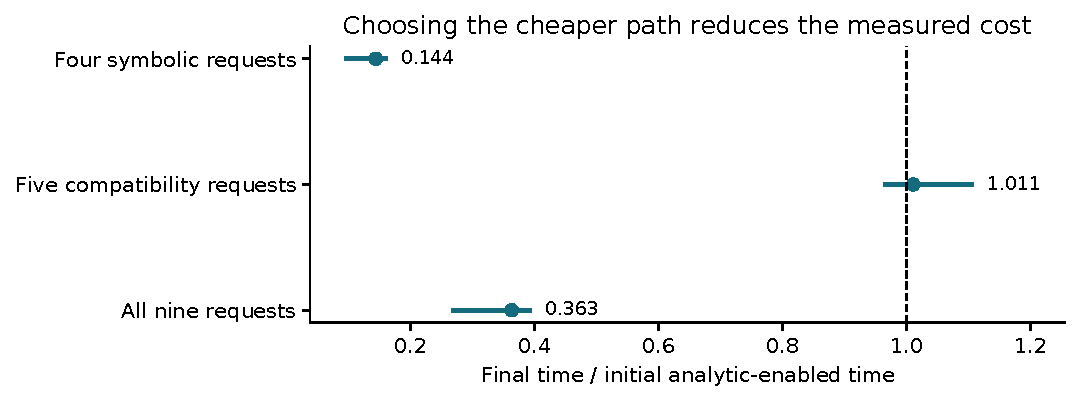
\includegraphics[width=.9\linewidth]{paper_figures/parser_guard.pdf}
\caption{The input rule bypasses symbolic recurrence work where native reduction is cheaper. Values below one favor the final rule. Intervals resample three repetitions on these fixed inputs. Compatibility requests check that other application branches remain available.}
\label{fig:notes-parser-guard}
\end{figure}

The final rule uses native Kira for the four symbolic requests, so their saving relative to the initial analytic variant is an integration improvement. This test compares complete paths and does not separately measure parsing, import, and symbolic arithmetic costs. It is not an additional ML contribution. The earlier 41-request experiment and this nine-request test use different targets and remain separate comparisons. We do not combine their times into a new overall speedup or claim that every symbolic family benefits from this rule.

\section{Inputs and admission rule for the final application}
\label{app:notes-parser-guard}
Use the symbolic two-point denominators $D_1=\ell^2-\mu_1+i0$ and $D_2=(\ell-p)^2-\mu_2+i0$, with independent variables $\mu_1$, $\mu_2$, and $s=p^2$. Development uses one target per request, with powers $(4,1)$ or $(1,4)$. Testing uses $(3,2)$ and $(2,3)$, one product of two identical $(3,2)$ blocks, and one product of thirteen identical $(2,3)$ blocks. As in the main comparison, identical blocks share work within each request and the product expansion stays factored.

The compatibility inputs comprise two-, four-, and five-denominator rational polygons at profile $2521$ and extra power three, using Appendix~\ref{app:notes-analytic-inputs}. They also include a nonplanar box at profile $2527$ with target $(1,1,1,1,1,1,1,-3,0)$ and the one-mass thirteen-loop vacuum at profile $2531$, with two extra powers on its first physical denominator. Their family definitions follow Appendices~\ref{app:hybrid-experts} and~\ref{app:families-new}. Every input uses the previously prepared master indices; the test does not add entries to that registry.

The input rule accepts direct integer or rational mass and scalar-product values for the new recurrence. Expressions that require a symbolic parser use the existing exact or native path, even if an expression could simplify to a rational number. This conservative implementation avoids a symbolic startup cost merely to decide which method to use. Three rotated repetitions compare the final learned application, its fixed counterpart, matched native settings, and the initial analytic-enabled application. Exact comparison with an independent reference follows every run and remains inside its timer.

% END CURRENT WORKFLOW UPDATE
% BEGIN CURRENT WORKFLOW UPDATE
\section{Reducing the cost of the exact stage}
\label{sec:notes-fast-method}
The preceding comparison shows that an exact formula can save algebraic work while still spending time on general symbolic setup. We therefore evaluate the finite products in the derived tadpole, one-mass vacuum, and massless propagator formulas directly. Their coefficients remain rational functions of the dimension and the permitted scales. The formulas include the supported quadratic numerators described in Appendix~\ref{app:blocks13}. Other numerator structures and coupled families pass to the existing reduction methods.

For scalar one-loop blocks, we also combine repeated terms before applying the recurrence in Eq.~\eqref{eq:notes-analytic-recurrence}. The coefficients are polynomials in $d$ with exact rational coefficients, so their arithmetic can use integer numerators and denominators throughout. Appendix~\ref{app:notes-fast-method} derives the combined recurrence. Independent blocks share this method, and repeated identical blocks share intermediate results within one request. No reduction coefficient from an earlier request enters a new answer.

Several raised indices can supply the next recurrence step. Each choice gives a valid decomposition, but the number of intermediate integrals can differ. We train a cost-sensitive tree to select among four strategies: choose the largest positive power, the smallest power greater than one, the first raised index, or the last raised index. A strategy applies at each intermediate integral. The model selects one strategy for the target collection before the exact recurrence begins; it does not predict a coefficient. The eleven inputs describe the number of denominators and targets, the extra positive powers, and the powers at the first five positions. Appendix~\ref{app:notes-fast-method} gives the features and training objective.

We measure all four strategies on 112 training requests and 56 separate validation requests. Each request contains one or two scalar targets with two through five denominators and at most six extra positive powers. Three repetitions provide a median recurrence time, and all strategies must agree exactly. Validation selects the tree and a minimum predicted saving, with the best fixed strategy as its control. These labels measure recurrence time plus prediction overhead. The reserved application comparison then tests whether the selected policy reduces total time after loading, basis checks, and output verification.

The resulting application first splits independent loop blocks, then attempts a direct formula or the scalar recurrence. It loads the existing learned Kira application when a block needs the remaining exact or native methods. This order reduces setup work on inputs with an immediate analytic decomposition. The retained sparse-seed model keeps its earlier weights. Learned row selection remains omitted, and the equation filter retains its separately tested application. The new recurrence policy adds a different decision to this combination.

Complete application validation also governs deployment of the recurrence model. Section~\ref{sec:notes-fast-deployment} measures that decision on the original validation split, freezes its outcome, and tests twelve fresh requests.

\section{Complete times and coverage through thirteen loops}
\label{sec:notes-fast-results}
The initial fast-implementation comparison tests the direct finite products, faster exact recurrence, and newly trained recurrence strategy together with the retained sparse-seed model. The preceding deployed application is the main practical control. A matched native control retains the earlier exact formulas and block splitting but uses native Kira decisions for the remaining work. The fast fixed control uses the new exact implementation and fixed choices. Thus the native control already contains acceleration, and its timing is not the time of stock Kira on every target.

The reserved set contains 65 requests, including analytic vacuum and propagator families at every loop count through thirteen, distinct triangle products, rational scalar polygons, symbolic bubbles, and coupled native cases. Appendix~\ref{app:notes-fast-inputs} defines the targets and parameter profiles. Each method starts a fresh process three times per completed request. The timer includes loading, prediction, exact reduction, output, and the independent coefficient check. Prepared master indices and reference calculations remain separate. Table~\ref{tab:notes-fast-results} compares only requests that complete every repetition for both methods.

\begin{table}[!htbp]\centering\small
\caption{Complete application times in the new reserved test. Times are sums of per-request medians in seconds. Each row uses the same matched requests for its three controls when all methods complete; any unequal counts are reported below.}
\label{tab:notes-fast-results}
\begin{tabularx}{\linewidth}{@{}Yrrrrr@{}}\toprule
Collection & $N$ & New learned & Previous & Native & Fast fixed\\\midrule
Vacuum and propagator formulas & 26 & 5.067 & 21.963 & 21.568 & 4.912 \\
Symbolic one-mass vacua & 4 & 0.750 & 2.728 & 2.705 & 0.791 \\
Distinct triangle products & 13 & 3.604 & 4.279 & 52.016 & 3.414 \\
Scalar recurrence & 9 & 2.733 & 8.716 & 15.223 & 2.727 \\
Nonplanar seed model & 8 & 39.518 & 38.883 & 66.601 & 42.392 \\
Symbolic native inputs & 2 & 1.608 & 1.269 & 1.448 & 1.574 \\
Coupled compatibility & 3 & 3.664 & 3.737 & 3.806 & 3.696 \\
All matched requests & 65 & 56.945 & 81.574 & 163.366 & 59.505 \\
\bottomrule\end{tabularx}\end{table}

The combined method uses 30.2\% less time than the preceding deployed application, with time ratio 0.698 and repetition interval $[0.676,0.717]$. The combined method uses 65.1\% less time than the already accelerated native control, with time ratio 0.349 and repetition interval $[0.338,0.360]$.

The combined method uses 4.3\% less time than the fast fixed control, with time ratio 0.957 and repetition interval $[0.925,0.986]$. This last comparison isolates request-dependent learned choices after the exact implementation changes. It does not assign the finite-product or arithmetic savings to ML.

The combined method completes 65 of 65 requests in all three repetitions. The preceding, native, and fast fixed methods complete 65, 65, and 65 requests, respectively. Independent reference preparation takes 432.328 seconds. Across the timed runs, the exact checker performs 12,180 coefficient comparisons. The new method's first-attempt total is 59.453 seconds, including 0.000 seconds spent on unverified or incomplete first attempts. Failed requests remain in these counts and receive no completed-time speedup.

\subsection{What the new learned decision adds}
The recurrence model selects a strategy before the exact substitutions begin. Validation chooses a depth-5 tree, minimum leaf population 3, and prediction margin 0.10. Its fixed alternative selects the last raised index. The measured validation recurrence total changes from 2.6229 to 2.5000 seconds, including prediction overhead. The reserved application test admits the new model on 22 requests and changes the fixed pivot strategy on 3 requests. These groups describe observed use, while the complete scalar-recurrence group was specified before testing.

For the nine reserved scalar-recurrence requests, the combined method uses 0.2\% more time than the same fast recurrence with fixed strategy, with time ratio 1.002 and repetition interval $[0.959,1.076]$. The interval includes equal times. For the eight nonplanar requests, the combined method uses 6.8\% less time than the fixed sparse-seed choice, with time ratio 0.932 and repetition interval $[0.888,0.961]$. The latter model retains its earlier training. These comparisons separate the new recurrence decision from the retained seed decision.

\begin{figure}[!htbp]\centering
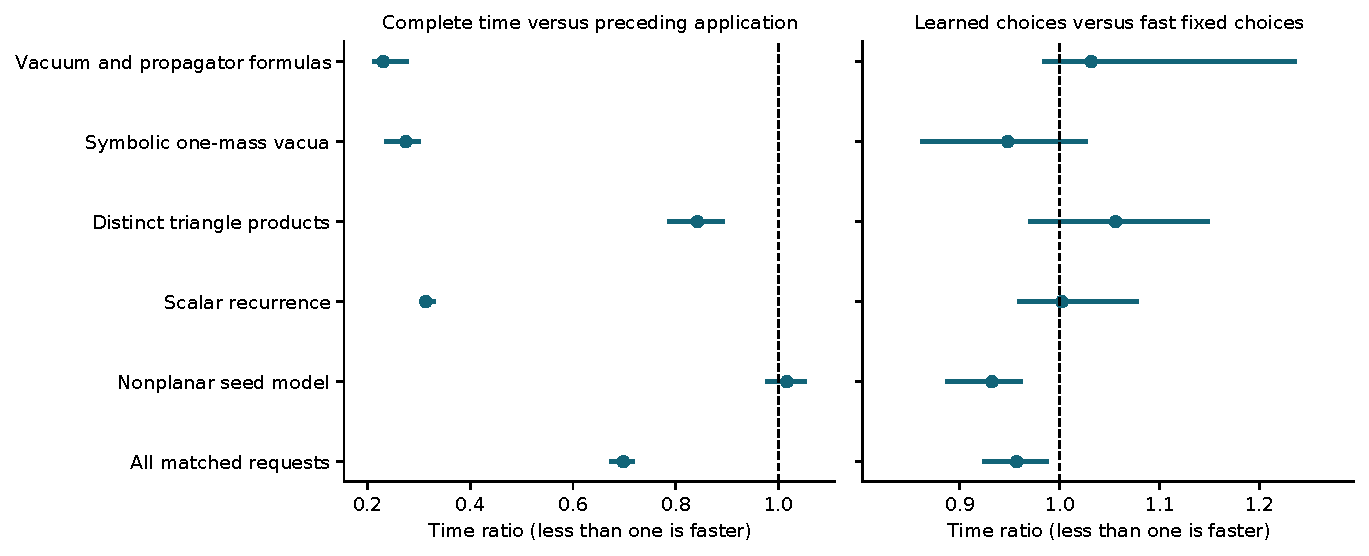
\includegraphics[width=\linewidth]{paper_figures/fast_decomposition.pdf}
\caption{Direct formulas and exact arithmetic reduce complete time, while the fixed control isolates the additional learned choices. Values below one favor the new learned application. Intervals resample the three paired repetitions on the same fixed requests. They do not measure uncertainty over all possible integral families. Formula-only groups use the same exact path in both methods, so their differences measure timing variation.}
\label{fig:notes-fast-time}
\end{figure}

\subsection{Which high-loop requests complete}
The timing set deliberately contains analytically supported families. To expose its limits, a separate 110-request audit includes one-mass and all-mass vacua, massless and massive propagators, scattering ladders, and boxes with bubble chains at each loop count through thirteen. It adds scaleless cases, other scattering structures, and symbolic scales. Each application receives twenty seconds per request. Figure~\ref{fig:notes-fast-coverage} shows the regular loop sequences, and Table~\ref{tab:notes-fast-coverage} includes every audit request.

\begin{table}[!htbp]\centering\small
\caption{Bounded audit at each loop count. ``New'' and ``Previous'' count reported completions within twenty seconds. ``Agree'' counts paired completions with exact coefficient agreement. The audit has different limits and targets from the timing comparison.}
\label{tab:notes-fast-coverage}
\begin{tabular}{@{}rrrrr@{}}\toprule
Loops & Requests & New & Previous & Agree\\\midrule
1 & 12 & 12 & 12 & 12 \\
2 & 12 & 12 & 12 & 12 \\
3 & 10 & 8 & 8 & 8 \\
4 & 7 & 4 & 4 & 4 \\
5 & 7 & 4 & 4 & 4 \\
6 & 10 & 5 & 5 & 5 \\
7 & 7 & 3 & 3 & 3 \\
8 & 7 & 3 & 2 & 2 \\
9 & 7 & 3 & 2 & 2 \\
10 & 7 & 3 & 2 & 2 \\
11 & 7 & 3 & 2 & 2 \\
12 & 7 & 3 & 2 & 2 \\
13 & 10 & 5 & 4 & 4 \\
Total & 110 & 68 & 62 & 62 \\
\bottomrule\end{tabular}\end{table}
\begin{figure}[!htbp]\centering
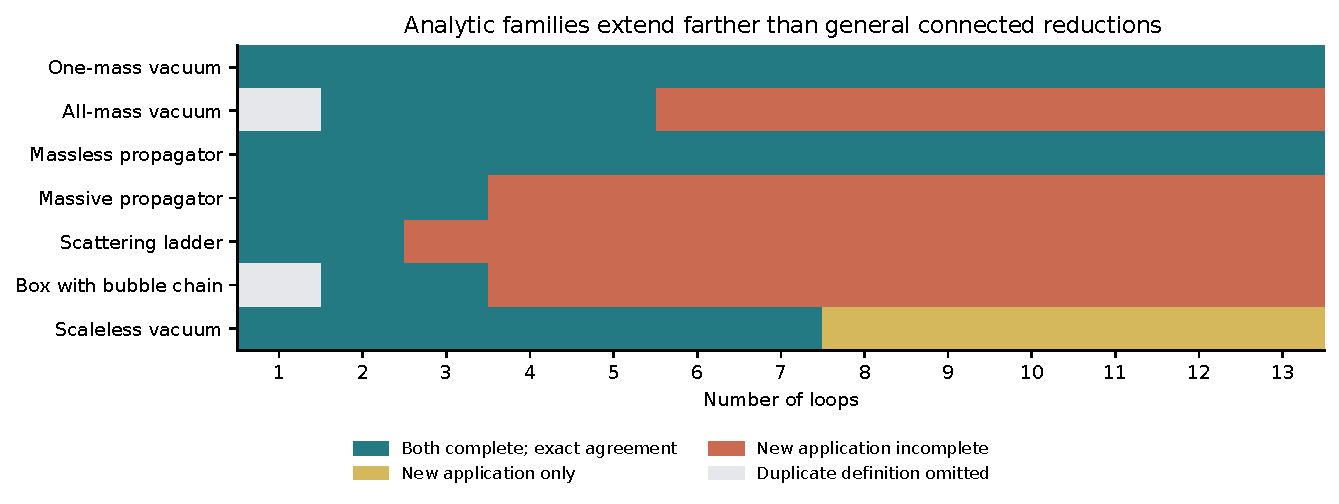
\includegraphics[width=\linewidth]{paper_figures/fast_coverage.pdf}
\caption{Completion depends on integral structure as well as loop count. The grid shows the new and preceding applications under the same twenty-second audit limit. A failed entry includes timeouts and unsupported inputs. Additional symbolic and scattering requests appear in the complete counts of Table~\ref{tab:notes-fast-coverage}.}
\label{fig:notes-fast-coverage}
\end{figure}
\FloatBarrier

The 42 incomplete requests comprise 12 time limits and 30 inputs above the native index bound.

The six additional completions are scaleless vacuum requests at eight through thirteen loops. Their exact result is zero by the homogeneous IBP identity derived in Eq.~\eqref{eq:notes-fast-scaleless}. The preceding application rejects their native index count before using this general zero rule. These additional completions come from an exact identity and carry no ML speedup claim.

The analytic families and independent products establish high-loop coverage within their derived domains. General coupled scattering, arbitrary numerator powers, singular kinematics, cut integrals, and symbolic indices require further methods or tests. The native 31-index limit also excludes some complete coupled coordinate systems~\cite{Kira3}. Neither prediction nor a shorter failed attempt supplies the missing reduction. The audit therefore records these limits explicitly and does not label its finite collection as all integral types.

\section{Combined recurrence and learned strategy}
\label{app:notes-fast-method}
For the target $\boldsymbol a=\boldsymbol b+\boldsymbol e_j$, define
\begin{equation}
 w_i=\frac{(Y_S^{-1})_{ji}}{b_j},\qquad
 W=\sum_{i\in S}w_i.
\end{equation}
Here $S$, $Y_S$, and $\boldsymbol b$ have the definitions in Appendix~\ref{app:notes-analytic-decomposition}. In the double sum of Eq.~\eqref{eq:notes-analytic-recurrence}, the term with $k=i$ has index vector $\boldsymbol b+\boldsymbol e_i-\boldsymbol e_i=\boldsymbol b$. Separating these terms gives
\begin{align}
 I_{\boldsymbol a}
 &= (d-B)W I_{\boldsymbol b}
    -\sum_{i\in S}w_i b_i I_{\boldsymbol b}
    -\sum_{\substack{i,k\in S\\k\ne i}}w_i b_k
       I_{\boldsymbol b+\boldsymbol e_k-\boldsymbol e_i}\\
 &=\left[(d-B)W-\sum_{i\in S}w_i b_i\right]I_{\boldsymbol b}
    -\sum_{\substack{i,k\in S\\k\ne i}}w_i b_k
       I_{\boldsymbol b+\boldsymbol e_k-\boldsymbol e_i}.
 \label{eq:notes-fast-recurrence}
\end{align}
This groups the coefficient of the same integral before further substitution. Its algebra, termination, and allowed master check are unchanged from the earlier recurrence. For rational kinematics, each $w_i$ is rational, so exact integer numerator and denominator arithmetic suffices. The dimension remains symbolic in the polynomial coefficient.

The direct scalar formulas use rising factorials. For $\Re z>0$, integration by parts in the defining gamma integral gives
\begin{equation}
 \Gamma(z+1)=[-t^ze^{-t}]_0^\infty
 +z\int_0^\infty t^{z-1}e^{-t}\,dt=z\Gamma(z).
\end{equation}
Here $t$ is the positive integration variable and $z$ is the complex argument. Applying this identity repeatedly gives
\begin{equation}
 (z)_n=\frac{\Gamma(z+n)}{\Gamma(z)}
      =\prod_{r=0}^{n-1}(z+r),\qquad (z)_0=1,
 \label{eq:notes-fast-product}
\end{equation}
for a nonnegative integer $n$. The equality extends by analytic continuation away from unresolved poles. Thus the ratios derived in Appendix~\ref{app:blocks13} can be evaluated through finite products without constructing gamma functions. The references use the earlier symbolic implementation, including gamma-function ratios for the multiloop vacuum and numerator requests. Scalar massless requests use its rising-factorial expression. The polygon recurrence uses independent native Kira reductions. This change concerns evaluation cost; it does not extend the mathematical domain of those formulas.

The scaleless-vacuum shortcut follows directly from IBP in dimensional regularization~\cite{ChetyrkinTkachov,Weinzierl2022}. With no masses or external momenta, every inverse propagator is homogeneous of degree two in the loop momenta. If $A=\sum_j a_j$, the product of propagator powers has degree $-2A$. Summing the IBP operators with $v=\ell_h$ therefore gives
\begin{equation}
 0=\int\prod_h\frac{d^d\ell_h}{i\pi^{d/2}}
 \sum_{h=1}^{L}\frac{\partial}{\partial\ell_h^\mu}
 \left(\ell_h^\mu\prod_j D_j^{-a_j}\right)
 =(Ld-2A)I_{\boldsymbol a}.
 \label{eq:notes-fast-scaleless}
\end{equation}
The factor $Ld-2A$ is nonzero at generic symbolic $d$, so the dimensionally regularized integral vanishes. Analytic continuation supplies the same scaleless result. This argument also permits negative integer powers because they preserve homogeneity. The six additional audit completions at eight through thirteen loops use this zero identity; they do not require a native system above its index limit.

For a target collection $\mathcal T$ with $q$ targets and $n$ denominator positions, define the extra positive power of target $\boldsymbol a$ by $\delta(\boldsymbol a)=\sum_{j=1}^{n}\max(a_j-1,0)$. The model inputs are
\begin{equation}
 \boldsymbol f=\left(n,q,\max_{\mathcal T}\delta,
 q^{-1}\sum_{\mathcal T}\delta,
 \max_{\boldsymbol a\in\mathcal T,j}a_j,
 \min_{\boldsymbol a\in\mathcal T}\sum_j\mathbf1_{a_j>0},
 \max_{\mathcal T}a_1,\ldots,\max_{\mathcal T}a_5\right).
 \label{eq:notes-fast-features}
\end{equation}
Absent positions have value zero. These are definitions of the representation, and $\mathbf1$ is the indicator function. Coordinate positions enter this small one-loop model; we do not claim invariance under arbitrary relabeling.

Let $t_{rc}$ be the median measured recurrence time for training request $r$ and strategy $c$. A leaf containing requests $R$ stores the four mean costs $|R|^{-1}\sum_{r\in R}t_{rc}$. We grow an axis-aligned regression tree using the tree framework of Ref.~\cite{CART1984}, with a cost-sensitive split criterion. For a proposed partition into $R_1$ and $R_2$, the minimized empirical action cost is
\begin{equation}
 J(R_1,R_2)=\sum_{u=1}^{2}\min_c\sum_{r\in R_u}t_{rc}.
 \label{eq:notes-fast-tree-loss}
\end{equation}
The equation follows by assigning one strategy to each leaf and summing its recorded costs. We accept a split only when it lowers this sum by more than $10^{-4}|R|$ seconds and satisfies the depth and population limits, where $|R|$ is the number of requests in the unsplit node. Candidate depths are one through five, and minimum leaf populations are three, six, or ten. Validation compares prediction margins $0$, $0.03$, and $0.10$ against the best single strategy. The selected model requires a two-percent aggregate validation saving and at least one changed decision before deployment.

For predicted costs $\widehat t_c$ and fixed strategy $c_0$, choose $c_*\in\arg\min_c\widehat t_c$. The application uses that change only when
\begin{equation}
 \widehat t_{c_*}+\tau < (1-\eta)\widehat t_{c_0},
 \qquad \tau=10^{-4}\ \mathrm{s},
 \label{eq:notes-fast-margin}
\end{equation}
where $\eta$ is the selected margin and $\tau$ allows for prediction work. Inputs outside the observed feature ranges use the fixed strategy. This rule is a design choice rather than a proof of a runtime improvement. Complete reserved timings measure its actual effect.

\section{Inputs for the extended comparison}
\label{app:notes-fast-inputs}
Training uses polygon kinematics at profiles $2611$ and $2617$, and validation uses profile $2621$. For each number of denominators $n=2,3,4,5$, each profile supplies fourteen target collections. Starting from unit powers, the generator distributes one through six extra powers among the denominator positions. Every third collection contains two targets, and the others contain one. The reserved profiles and target collections below are separate.

The timing set contains 65 requests. At each loop count $L=1,\ldots,13$, it includes a one-mass vacuum banana and a massless propagator banana from Appendix~\ref{app:families-new}, with profile $2701+2L$. It also includes a product of $L$ independent massive triangles. Each triangle uses the polygon kinematics of Appendix~\ref{app:notes-analytic-inputs} at profile $2741$, adds $7b+L$ to each squared mass for block $b=0,\ldots,L-1$, and has target powers $(2,1,1)$. These distinct masses require separate block reductions within a request.

Four further one-mass vacuum requests keep their scale symbolic at $L=1,2,6,13$. Nine scalar recurrence requests use polygons with $n=3,4,5$ at profile $2777$ and powers $(3,2,1,\ldots,1)$, $(1,\ldots,1,2,3)$, or $(2,\ldots,2)$. Two fully symbolic bubbles use profile $2783$ with the two power collections defined in Appendix~\ref{app:notes-analytic-inputs}. Eight nonplanar-box requests at profile $2791$ use unit physical powers and the auxiliary pairs $(-2,0)$, $(0,-2)$, $(-3,0)$, $(0,-3)$, $(-2,-1)$, $(-4,0)$, $(0,-4)$, and $(-2,-2)$. Three compatibility requests use a massive two-loop propagator, an all-mass three-loop vacuum, and a two-loop ladder at profile $2797$, with the first physical power raised by one.

A separate 110-request audit tests the six vacuum, propagator, and scattering sequences of Appendix~\ref{app:families-new} at each loop count through thirteen, excluding two duplicate one-loop definitions. It adds thirteen scaleless vacuum requests, six scattering requests with mixed or pinched powers, and fifteen symbolic-scale requests. Both the preceding and new application receive a twenty-second limit for each audit request. The audit records exact agreement when both complete, as well as time limits, missing basis support, and native input limits. These bounded outcomes do not prove that a failed integral has no reduction.

The native solver used here has a documented maximum of 31 integral indices~\cite{Kira3}. A complete independent scalar-product coordinate system has $L(L+1)/2+LE$ entries for $E$ external momenta, from the $L(L+1)/2$ symmetric loop--loop products and $LE$ loop--external products. Analytic formulas and independent blocks can handle some requests above this native bound. A coupled request outside both the exact domain and the native limit remains unsupported. The finite audit also leaves arbitrary numerators, singular kinematics, cut propagators, and symbolic propagator powers outside a universal coverage claim.

% END CURRENT WORKFLOW UPDATE
% BEGIN CURRENT WORKFLOW UPDATE
\section{Selecting the final application by complete time}
\label{sec:notes-fast-deployment}
We selected the new tree using recurrence times. A lower kernel cost alone does not establish a lower application cost, so deployment requires a further check on the original validation split. We run the same 56 validation requests in fresh processes, with prediction, exact reduction, and coefficient comparison inside each timer. The two choices use the same fast implementation and retain the same native seed model; they differ only in the recurrence strategy. Three paired repetitions provide each request's median time. We enable the new recurrence model only when its summed median time is at least two percent lower and its paired repetition interval stays below one. The 65 reserved requests do not enter this decision.

The complete validation total is 13.282 seconds with the recurrence model and 13.408 seconds with the fixed strategy. The ratio is 0.991, with repetition interval $[0.953,1.015]$. The final application therefore uses the fixed recurrence strategy. The kernel saving does not meet the complete-time deployment rule, so the trained tree remains a recorded candidate. The retained sparse-seed model remains active in its validated coupled domain. This decision leaves all exact formulas and coefficient checks unchanged.

A separate twelve-request test follows the frozen decision. It includes six rational polygons, two distinct-triangle products at two and thirteen loops, a nonplanar box, a symbolic bubble, and two thirteen-loop analytic families. Appendix~\ref{app:notes-fast-deployment} specifies their fresh inputs. Table~\ref{tab:notes-fast-deployment} keeps this test separate from the preceding 65-request experiment.
\begin{table}[!htbp]\centering\small
\caption{Separate reserved test of the final complete-cost rule. Times are sums of medians in seconds. ``Candidate'' always enables the recurrence model. ``Fixed recurrence'' retains the native seed model but uses the fixed recurrence strategy.}
\label{tab:notes-fast-deployment}
\begin{tabularx}{\linewidth}{@{}Yrrrrr@{}}\toprule
Collection & $N$ & Final & Candidate & Fixed recurrence & Previous\\\midrule
Scalar recurrence & 6 & 1.708 & 1.670 & 1.756 & 4.125 \\
Distinct products & 2 & 0.614 & 0.600 & 0.598 & 0.791 \\
Nonplanar box & 1 & 3.856 & 3.719 & 3.818 & 3.955 \\
Symbolic bubble & 1 & 0.699 & 0.737 & 0.724 & 0.704 \\
Thirteen-loop formulas & 2 & 0.377 & 0.323 & 0.351 & 1.763 \\
All requests & 12 & 7.254 & 7.048 & 7.248 & 11.338 \\
\bottomrule\end{tabularx}\end{table}

Against the preceding deployed application, the final method uses 36.0\% less time, with ratio 0.640 and repetition interval $[0.612,0.712]$. Against the always-enabled recurrence candidate, the final method uses 2.9\% more time, with ratio 1.029 and repetition interval $[0.981,1.131]$. This interval includes equal times. Against the fixed recurrence strategy, the final method uses 0.1\% more time, with ratio 1.001 and repetition interval $[0.951,1.118]$. This interval includes equal times.

The final method completes 12 of twelve requests in every repetition. All verified outputs agree with the independent references, with 2,856 coefficient comparisons in this test and 6,072 in the full-cost validation. Reference preparation for the twelve requests takes 73.895 seconds and remains separate. The broad audit in the preceding section belongs to the initial candidate. The final test checks the deployment rule on fresh inputs, while the earlier audit retains its original outcomes and native limits.

\section{Inputs for the complete-cost deployment test}
\label{app:notes-fast-deployment}
Use the polygon definitions of Appendix~\ref{app:notes-analytic-inputs} with profile $2917$, $n=3,4,5$, and powers $(3,2,1,\ldots,1)$ or $(1,\ldots,1,2,3)$. The distinct-triangle products contain two or thirteen blocks at profile $2927$, with the mass offsets and target $(2,1,1)$ defined in Appendix~\ref{app:notes-fast-inputs}. The nonplanar box has profile $2939$ and auxiliary powers $(-3,0)$. The symbolic bubble has profile $2941$ and the first extra-power collection of Appendix~\ref{app:notes-analytic-inputs}. The one-mass vacuum and massless propagator families have thirteen loops and profile $2953$.

The full-cost admission uses only the original profile-$2621$ validation inputs. Its cost includes a fresh process, the learned or fixed choice, exact recurrence, output, and comparison with the earlier exact scalar recurrence. The additional reserved references use the same independent native and analytic checks as the main test. We fix all source choices and the admission result before these twelve requests run. The final rule changes no fitted weights. It selects whether the recurrence model earns its cost in the complete application.

% END CURRENT WORKFLOW UPDATE
% BEGIN CURRENT WORKFLOW UPDATE
\section{Exact triangle reduction and learned target grouping}
\label{sec:notes-analytic-batch-method}
Some integral structures admit a direct reduction formula. We use such a formula before asking a learned model to choose the remaining native work. The new exact case is a massless one-loop triangle with two lightlike external momenta and one nonzero invariant. Its denominator powers can include a polynomial numerator. Its singular invariant matrix prevents use of the preceding inverse-matrix recurrence in the full triangle sector. Appendix~\ref{app:notes-analytic-batch} derives the coefficient of a single off-shell bubble master from Feynman parameters and expresses it through finite products. This avoids equation generation and elimination for that block. Factorization then applies the formula independently to products of these blocks. The tests through thirteen loops concern these independent products; they do not establish a formula for a general connected thirteen-loop scattering graph.

For the coupled two-loop boxes, several requested integrals often need overlapping equations. We therefore train a model to select how Kira shares the reduction work. The five choices are the preceding application, a common reduction with either of two sparse seed regions, separate reductions for groups of equal numerator rank, and separate reductions for each target. Numerator rank is the sum of the absolute values of negative indices. Each choice uses the same target integrals and checked master basis. Exact algebra determines the coefficients, and an incomplete restricted reduction invokes the existing recovery procedure.

The model uses seventeen numerical features of the denominators and target indices. These include target count, numerator ranks, distances between numerator indices, and how propagators depend on the loop momenta. It predicts the complete cost of each choice. A cost-sensitive tree selects splits that reduce the sum of measured action costs, and bootstrap ensembles provide an additional candidate model~\cite{CART1984,Breiman1996Bagging}. Appendix~\ref{app:notes-analytic-batch} derives the training objective and states all candidate settings. Reference coefficients enter only the independent result checks.

We collect 32 training requests and sixteen separate validation requests from planar and nonplanar massless boxes. Their indices have unit positive propagator powers and numerator ranks one through four. We select the model using validation costs, then test its full application cost against the best fixed action at a fresh validation profile. This second check includes loading, prediction, exact reduction, and verification. The model enters deployment only if it saves at least two percent, completes every validation check, and has a request-resampling interval below equal time. The reserved requests remain unused during both decisions.

During development, repeated basis discovery caused avoidable failures on some planar batches. We add a separately checked registry containing only master indices. Two native reductions with different integral orderings must reproduce each other and the development coefficients. The same-basis control receives this registry too, so it separates basis preparation from the new triangle formula and learned grouping. The unmodified preceding application supplies a further practical control. We report basis preparation and benchmark-reference preparation separately from the supplied-basis application timer.

\section{Complete-time results for exact triangles and target batches}
\label{sec:notes-analytic-batch-results}
The reserved comparison contains forty native two-loop box requests, thirteen independent triangle products, one triangle with a symbolic scale, and four compatibility requests. Thirty-two box requests use fresh kinematics with the original index patterns, while eight use new index batches. The compatibility requests retain the earlier vacuum, propagator, and ladder definitions. Appendix~\ref{app:notes-analytic-batch} specifies every collection and the separation between training, validation, and testing.

Each measurement starts a fresh application process and includes loading, model use, exact reduction, retries, output, and the independent coefficient comparison. Three repetitions rotate method order on each request's worker. A first unverified result remains recorded and stops further repetitions for that method and request. Completed-time ratios include only requests verified by both compared methods; the separate completion table retains all requests.

The reserved measurements use two single-core workers on the same Intel(R) Xeon(R) Gold 6240 CPU @ 2.60GHz compute node. We fix that hardware assignment before the reserved tests. The full application validation uses a fresh profile on the same hardware. We preserve an interrupted heterogeneous-worker comparison in the notes; those trials do not determine admission. Each request compares every method on the same worker. The cluster allocation shares the node with other work, and the reported repetition intervals describe variation under those conditions.

Training selects 1 tree with maximum depth 4 and minimum leaf population 2. The full application validation takes 45.942 seconds with the selected policy and 49.598 seconds with the fixed action. Its time ratio is 0.926, with request-resampling interval $[0.853,0.995]$. The deployment rule therefore enables the new batch model. The separate reserved comparisons below measure the added learned choice after this decision.

The selected fixed action is the wider shared sparse region. The tree changes that action only when its predicted saving exceeds 8\% of the fixed cost plus 0.002 seconds. It changes the fixed action on 3 model-selection requests and makes a prediction on 38 reserved requests within its input ranges. Exact formulas and the preceding application handle the remaining structures or inputs outside those ranges.

Within those reserved predictions, the model selects the tighter shared sparse region on 7 requests and the wider shared sparse region on 31 requests. These observed choices show which alternatives contribute to the deployed result.

\begin{table}[!htbp]\centering\small
\caption{Complete-time comparison with the preceding application supplied with the same checked master indices. Times are sums of request medians in seconds. Each row uses only pairs that pass all three repetitions. A ratio below one means less time.}
\label{tab:notes-analytic-batch-times}
\begin{tabularx}{\linewidth}{@{}Yrrrr@{}}\toprule
Collection & Pairs & New & Same-basis control & Ratio\\\midrule
Planar box batches & 16 & 27.549 & 46.252 & 0.596 \\
Nonplanar box batches & 16 & 65.740 & 96.545 & 0.681 \\
New index batches & 8 & 35.722 & 44.213 & 0.808 \\
Triangle products, one to thirteen loops & 13 & 2.540 & 29.240 & 0.087 \\
Triangle with symbolic scale & 1 & 0.255 & 0.642 & 0.397 \\
Compatibility requests & 4 & 2.313 & 2.384 & 0.970 \\
All matched requests & 58 & 134.119 & 219.277 & 0.612 \\
\bottomrule\end{tabularx}\end{table}

Against the preceding method with the same basis, the final method uses 38.8\% less time on 58 matched requests. The ratio is 0.612, with repetition interval $[0.604,0.623]$. The new method is slower on 8 of those individual requests; the largest individual time ratio is 1.157. These per-request outcomes remain visible in the full result record.

Against the unmodified preceding application, the final method uses 67.6\% less time on 52 matched requests. The ratio is 0.324, with repetition interval $[0.321,0.331]$. The matched populations can differ because failed requests remain outside a completed-time ratio. Their totals therefore cannot be subtracted to assign a basis-preparation saving.

\begin{table}[!htbp]\centering\small
\caption{Added effect of the new batch decision on native requests. The fixed control has the same exact methods and basis, with the new model disabled. Both methods retain the preceding sparse expert where its action calls for it. These are original measurements of this study.}
\label{tab:notes-analytic-batch-ml}
\begin{tabularx}{\linewidth}{@{}Yrrrr@{}}\toprule
Collection & Pairs & Final time & Fixed time & Ratio\\\midrule
Planar box batches & 16 & 27.549 & 28.864 & 0.954 \\
Nonplanar box batches & 16 & 65.740 & 71.957 & 0.914 \\
New index batches & 8 & 35.722 & 31.725 & 1.126 \\
All native box batches & 40 & 129.010 & 132.546 & 0.973 \\
\bottomrule\end{tabularx}\end{table}

Against the fixed batch action over the forty native box requests, the final method uses 2.7\% less time on 40 matched requests. The ratio is 0.973, with repetition interval $[0.962,0.989]$. This subtotal isolates the added model on the native workload. The full-workflow comparisons below also retain exact and compatibility requests.

The learned choice takes more time on 19 individual native requests, with a largest request ratio of 2.386. Its aggregate saving therefore does not imply a saving for each input. The recorded native elimination counters total 3,155,328 operations for the learned choice and 3,449,687 for the fixed action. These counters cover the instrumented native algebra; they exclude loading, symbolic checks, and direct-formula arithmetic. The complete timer includes those costs.

Against the same workflow with a fixed batch action, the final method uses 2.5\% less time on 58 matched requests. The ratio is 0.975, with repetition interval $[0.961,0.994]$. Against the same workflow with both learned choices disabled, the final method uses 1.9\% less time on 58 matched requests. The ratio is 0.981, with repetition interval $[0.972,0.999]$. The second control changes the earlier seed choice as well, so its difference measures the combined learned decisions.

\begin{figure}[!htbp]\centering
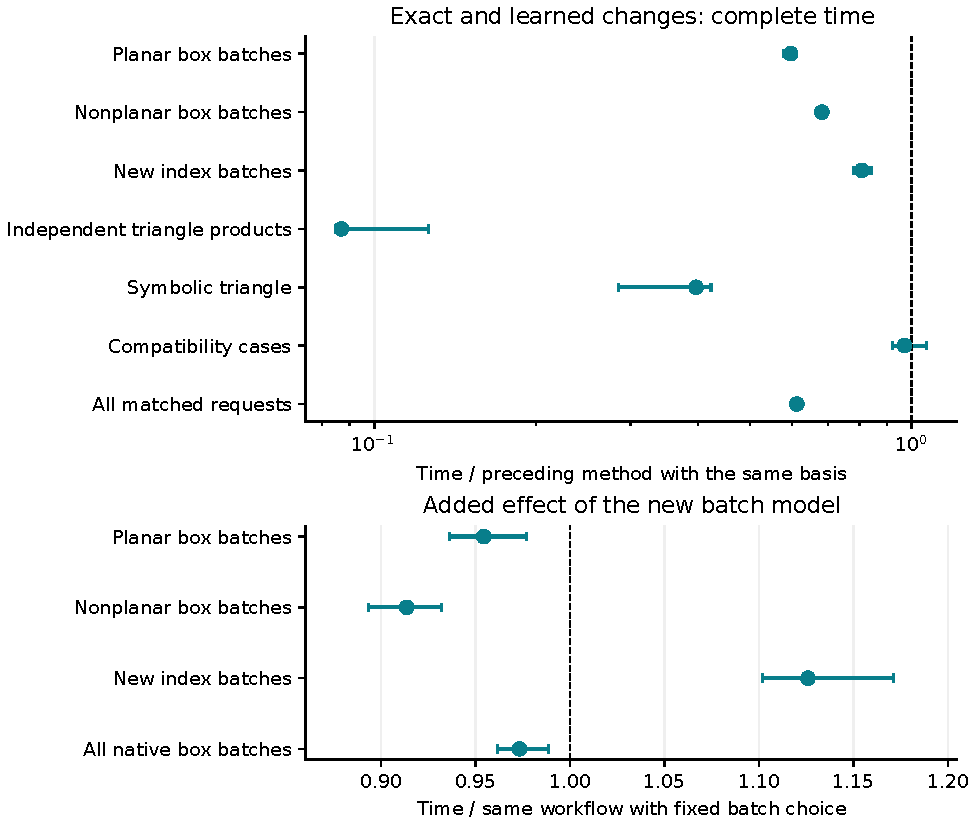
\includegraphics[width=\linewidth]{paper_figures/analytic_batch.pdf}
\caption{The upper panel measures the combined analytic and learned changes with matched basis preparation. Its logarithmic axis accommodates the exact-triangle saving and the smaller native changes. The lower panel isolates the new batch choice within the native test groups. Horizontal intervals describe paired repetition variation. The line at one indicates equal time; completion counts appear separately in Table~\ref{tab:notes-analytic-batch-completion}.}
\label{fig:notes-analytic-batch}
\end{figure}
\begin{table}[!htbp]\centering\small
\caption{Completion and first-pass cost over all 58 reserved requests. A verified request must pass all three repetitions. First-pass time sums the first measured application and check cost for every request, including failed work. The paired completed-time ratios appear in Table~\ref{tab:notes-analytic-batch-times}.}
\label{tab:notes-analytic-batch-completion}
\begin{tabularx}{\linewidth}{@{}Yrrr@{}}\toprule
Method & Verified & First unverified & First-pass seconds\\\midrule
Final method & 58 & 0 & 135.430 \\
Fixed batch action & 58 & 0 & 139.245 \\
Both learned choices disabled & 58 & 0 & 137.895 \\
Preceding method, same basis & 58 & 0 & 220.267 \\
Unmodified preceding application & 52 & 6 & 597.327 \\
\bottomrule\end{tabularx}\end{table}

The reserved test contains 858 measured outcomes and 14,226 successful coefficient comparisons. The added basis preparation takes 15.747 seconds and supplies 126 coefficient checks across five development requests. Independent reference preparation for the reserved set takes 237.539 seconds. These one-time and benchmark costs remain separate from the supplied-basis totals. The stored master indices contain no solved target coefficients.

Training-data collection, model selection data, and full-cost admission use 1663.451 seconds of summed measured application time. Their independent references add 261.918 seconds. These are separate one-time learning costs. The reserved reduction times measure use of the prepared method and do not imply that training has already paid for itself in a single calculation. Summed process times also differ from elapsed collection time when two workers run concurrently.

The triangle identity has an explicit analytic domain and independent native checks. The learned model has a narrower measured domain: two massless two-loop box structures with rational kinematics and symbolic dimension. The new index batches test transfer within those structures. General connected higher-loop scattering and all integral types remain outside this evidence. A finite candidate search also cannot prove that the selected workflow has the smallest possible runtime.
\FloatBarrier
\subsection{Preserved validation before the hardware assignment}
The initial full application validation used profile $3037$ on two different cluster nodes. It recorded 79 completed measurements with exact agreement before the slower worker was stopped. Their summed measured time is 606.267 seconds. The runtime and measurement sources, completed records, and interrupted inputs remain preserved. These measurements do not enter the admission decision. We retain the selected tree and its weights, then use the fresh profile $3041$ on the fixed reserved-test node for the completed validation. This change precedes all reserved testing and changes no target reduction formula.

\section{Exact one-scale triangles and shared target reductions}
\label{app:notes-analytic-batch}

The new exact rule applies to a massless triangle whose two adjacent external momenta satisfy
\(p_1^2=p_2^2=0\), while \(s=(p_1+p_2)^2\ne0\). We use the same Minkowski denominator convention as the preceding integral definitions and write
\begin{equation}
 T(a,b,c)=\int\frac{\mathrm d^d\ell}{i\pi^{d/2}}\,
 \frac{1}{[\ell^2+i0]^a[(\ell-p_1)^2+i0]^b
 [(\ell-p_1-p_2)^2+i0]^c},
 \qquad \mathcal B(s,d)=T(1,0,1).
 \label{eq:notes-batch-triangle-definition}
\end{equation}
Here \(a,b,c\) are integer propagator powers and \(\mathcal B(s,d)\) is the off-shell bubble master integral. The rule keeps \(d\) symbolic. It does not evaluate the master integral numerically.

Substituting the three external shifts and zero internal masses into Eq.~\eqref{eq:notes-analytic-y} gives
\begin{equation}
 Y=\begin{pmatrix}0&0&-s\\0&0&0\\-s&0&0\end{pmatrix},
 \qquad \det Y=0.
 \label{eq:notes-batch-triangle-matrix}
\end{equation}
The zero middle row makes the full triangle matrix singular. The preceding recurrence requires its inverse, so this sector needs another identity. The parameter integral below provides that identity directly.

Let \(A=a+b+c\). Feynman parametrization and the loop-momentum integral give the standard simplex representation \cite{Weinzierl2022}. For this triangle the quadratic form is \(-s x_1x_3-i0\), so the representation becomes
\begin{align}
 T(a,b,c)
 &=
 \frac{(-1)^A\Gamma(A-d/2)}{\Gamma(a)\Gamma(b)\Gamma(c)}
 (-s-i0)^{d/2-A}
 \int_{x_j\ge0}\!\mathrm dx_1\,\mathrm dx_2\,\mathrm dx_3\,
 \delta(1-x_1-x_2-x_3)
 \nonumber\\[-2pt]
 &\hspace{30mm}\times
 x_1^{d/2-b-c-1}x_2^{b-1}x_3^{d/2-a-b-1}.
 \label{eq:notes-batch-triangle-simplex}
\end{align}
We first take powers and dimension in a convergence domain and then continue the result meromorphically. Here \(\Gamma\) is Euler's gamma function. Its integral definition gives a useful relation for the parameter integrals:
\begin{align}
 \Gamma(\alpha)\Gamma(\beta)
 &=\int_0^\infty\!\mathrm dt\int_0^\infty\!\mathrm dr\,
 t^{\alpha-1}r^{\beta-1}e^{-t-r}
 \nonumber\\
 &=\Gamma(\alpha+\beta)
 \int_0^1\!\mathrm dz\,z^{\alpha-1}(1-z)^{\beta-1}.
 \label{eq:notes-batch-beta}
\end{align}
The second line follows from \(\rho=t+r\), \(z=t/(t+r)\), and the Jacobian \(\rho\). The \(\rho\) integral equals \(\Gamma(\alpha+\beta)\), which derives the beta integral in terms of gamma functions. To evaluate the simplex integral, set \(x_1=u\), \(x_2=(1-u)v\), and \(x_3=(1-u)(1-v)\). The Jacobian is \(1-u\), and two applications of Eq.~\eqref{eq:notes-batch-beta} give
\begin{equation}
 \int\!\mathrm d^3x\,\delta(1-\textstyle\sum_jx_j)
 \prod_{j=1}^3x_j^{\alpha_j-1}
 =
 \frac{\Gamma(\alpha_1)\Gamma(\alpha_2)\Gamma(\alpha_3)}
 {\Gamma(\alpha_1+\alpha_2+\alpha_3)}.
 \label{eq:notes-batch-dirichlet}
\end{equation}
The three exponents in Eq.~\eqref{eq:notes-batch-triangle-simplex} correspond to
\(\alpha_1=d/2-b-c\), \(\alpha_2=b\), and \(\alpha_3=d/2-a-b\). Substitution cancels \(\Gamma(b)\) and yields
\begin{equation}
 T(a,b,c)=
 (-1)^A(-s-i0)^{d/2-A}
 \frac{\Gamma(A-d/2)\Gamma(d/2-a-b)\Gamma(d/2-b-c)}
 {\Gamma(a)\Gamma(c)\Gamma(d-A)}.
 \label{eq:notes-batch-triangle-gamma}
\end{equation}
The same continued expression supplies \(b=0\) and negative integer \(b\), where the middle inverse propagator appears in the numerator. The native checks include these cases. When \(a\le0\) or \(c\le0\), the remaining loop denominators carry only a lightlike external momentum. Tensor expansion of the polynomial numerator then leaves scaleless integrals, which vanish in dimensional regularization \cite{Weinzierl2022}.

For \(a,c\ge1\), set \(\Delta=A-2\) and divide Eq.~\eqref{eq:notes-batch-triangle-gamma} by its value at \((1,0,1)\):
\begin{align}
 \frac{T(a,b,c)}{\mathcal B(s,d)}
 ={}&
 \frac{s^{-\Delta}}{(a-1)!(c-1)!}
 \frac{\Gamma(2-d/2+\Delta)}{\Gamma(2-d/2)}
 \frac{\Gamma(d/2-a-b)}{\Gamma(d/2-1)}
 \nonumber\\
 &\times
 \frac{\Gamma(d/2-b-c)}{\Gamma(d/2-1)}
 \frac{\Gamma(d-2)}{\Gamma(d-2-\Delta)}.
 \label{eq:notes-batch-triangle-ratio}
\end{align}
The integer power \(\Delta\) makes the signs from \((-1)^\Delta\) and \((-s)^{-\Delta}\) cancel. Every gamma-function argument differs from its denominator argument by an integer. Repeated application of \(\Gamma(z+1)=z\Gamma(z)\), used in Appendix~\ref{app:notes-fast-method}, therefore gives
\begin{equation}
 G(z,n)=\frac{\Gamma(z+n)}{\Gamma(z)}
 =
 \begin{cases}
 \displaystyle\prod_{j=0}^{n-1}(z+j),&n\ge0,\\[4pt]
 \displaystyle\left[\prod_{j=1}^{-n}(z-j)\right]^{-1},&n<0 .
 \end{cases}
 \label{eq:notes-batch-gamma-shift}
\end{equation}
The empty product equals one. These finite products express every tested triangle coefficient as a rational function of \(d\) and \(s\). The method needs no seed prediction or elimination sequence within this domain. Independent loop blocks use the factorization derived earlier in the paper.

The learned decision concerns the native reductions that remain. For a target set \(\mathcal T\), we compare the preceding application, two shared sparse seed regions, groups with equal numerator rank, and separate target reductions. All choices use exact IBP relations. A shared reduction solves the common equations once and reads the rows for every target. If
\begin{equation}
 I_{\mathbf a}=\sum_m r_{\mathbf a m}M_m
 \quad(\mathbf a\in\mathcal T),
 \qquad
 \mathbf I_{\mathcal T}=R_{\mathcal T}\mathbf M,
 \label{eq:notes-batch-shared}
\end{equation}
then selecting several rows of \(R_{\mathcal T}\) requires the same master basis \(\mathbf M\). Sharing the equations changes the work needed to construct these rows; it preserves each reduction identity.

The sparse regions extend the earlier seed rule to a union over the requested targets. In a sector \(S\), let \(a_j\le0\) denote a seed numerator power at an absent denominator. Its distance from a target's numerator box is
\begin{equation}
 D_S(\mathbf a,\mathbf t)
 =\sum_{j\notin S}\max\!\left(0,-a_j-\max(0,-t_j)\right).
 \label{eq:notes-batch-seed-distance}
\end{equation}
The shared region retains a seed when the smallest distance over \(\mathbf t\in\mathcal T\) lies within the selected radius. It also keeps admissible target and master seeds and applies the native rank and propagator bounds. The two tested radii and bound parameters are fixed before collection. If the selected seed set does not complete the requested reduction, the existing recovery procedure expands the native calculation.

We train the policy from complete measured time. Let \(C_{ia}\) be the measured cost of choice \(a\) on training request \(i\), including the fresh process, reduction, recovery, and exact coefficient comparison. An unsuccessful result receives a cost of at least \(250\) seconds. A leaf with request set \(S\) predicts
\begin{equation}
 \widehat C_a(S)=\frac{1}{|S|}\sum_{i\in S}C_{ia}.
 \label{eq:notes-batch-leaf-cost}
\end{equation}
If a split creates \(S_L\) and \(S_R\), the least recorded cost available to its two leaves is
\begin{equation}
 \mathcal L(S_L,S_R)=
 \min_a\sum_{i\in S_L}C_{ia}
 +\min_a\sum_{i\in S_R}C_{ia}.
 \label{eq:notes-batch-tree-loss}
\end{equation}
This follows by choosing one action independently in each leaf. We use this cost-sensitive form of recursive tree construction and also test bootstrap ensembles \cite{CART1984,Breiman1996Bagging}. Prediction averages the action costs across the selected trees. Validation selects the model, its margin over a fixed choice, and whether the complete application should enable it.

The model receives seventeen structural quantities: loop count, external-momentum count, total denominator count, physical denominator count, target count, minimum, maximum, and mean numerator rank, number of distinct ranks, maximum number of extra positive propagator powers, minimum active-line count, largest numerator power, maximum and mean pairwise numerator-index distance, largest number of active numerator positions, number of propagators that contain both loop momenta, and largest loop-momentum incidence count. The pairwise distance is the sum of absolute differences over auxiliary indices. These quantities describe the requested algebra and do not contain reference coefficients or family names. The measured learning domain consists of two-loop, seven-line, nine-index requests with numerator rank one through four. The independent-product tests through thirteen loops assess the exact method separately.


\subsection{Training inputs, controls, and basis preparation}
The native learning data use the planar and nonplanar massless boxes defined in Appendix~\ref{app:families-new}. Their first seven indices equal one. We write the last two indices as $(-u,-v)$ and use these eight target collections for each graph and parameter profile:
\begin{align*}
 &\{(2,0)\},\quad \{(0,3)\},\quad \{(2,1)\},\quad
 \{(2,0),(0,2)\},\\
 &\{(3,0),(0,3),(2,1)\},\quad \{(2,0),(0,3)\},\\
 &\{(1,0),(2,0),(3,0),(4,0)\},\quad
 \{(1,1),(2,1),(1,2),(2,2)\}.
\end{align*}
Profiles $3011$ and $3019$ supply 32 training requests, while profile $3037$ supplies sixteen validation requests. For profile $h$, the planar invariants are $s=-1009-12h$ and $t=-1021-14h$. The nonplanar convention uses $s=-113-18h$ and $t=-127-10h$, with the scalar products defined in Appendix~\ref{app:families-new}. Each training action runs once and each validation action runs twice. Candidate trees have depths one through four and minimum leaf populations of two, four, or eight. Ensembles contain sixteen bootstrap trees, and a single tree provides the other candidate. We test margins of zero, three, and eight percent against the validation-selected fixed action. A further three-repeat, fresh-process validation at the new profile $3041$ compares the selected model with the fixed action. We assign this validation and the reserved tests to the same compute node before they run. An interrupted validation on heterogeneous workers remains in the notes and does not determine admission. The model enters deployment only if it passes all exact checks, saves at least two percent in this full application comparison, and has an upper paired request-resampling ratio below one. All these decisions precede the reserved test.

The two sparse choices use the boundary vectors
$(2.5,0,0,1.25,0,1,-0.25)$ and $(1,0,0,0,1,1,0)$ in the earlier sparse-radius definition. Both use the native subsector rank truncation with one additional numerator rank. Rank grouping uses the second vector within each group. Single-target reduction and the preceding-application action preserve the earlier validated choices. The first four physical and structural feature counts are constant within this learning set, so their presence does not establish extrapolation in those quantities.

During development, repeated master discovery caused some planar batches to exceed the application limit. We therefore prepare an additional master-index registry. For three planar target collections and the rational and symbolic triangles, two native reductions with different integral orderings must agree exactly with each other and with the development reference. The planar collections must give the same canonical master-index set. The registry stores those indices and supplies no reduction coefficients. It can therefore remove repeated basis discovery while still requiring a new reduction at each kinematic point. Its preparation time is reported separately. Agreement on these checks establishes consistency for the tested inputs; it does not prove that a finite seed region finds the minimal basis for every kinematic specialization.

The reserved native test uses profiles $3053$ and $3061$, giving 32 requests from the original target collections. Eight further requests use profile $3067$ and the new collections
\[
 \{(1,2)\},\qquad\{(3,1)\},\qquad
 \{(2,0),(1,1),(0,2)\},\qquad
 \{(0,1),(1,1),(1,2),(1,3)\}.
\]
Both graphs receive each new collection. These are new index batches within two known graphs. They do not test a previously unseen connected topology.

The exact tests contain one independent triangle product at every loop order $L=1,\ldots,13$. Block $j=0,\ldots,L-1$ has powers
\[
 (a_j,b_j,c_j)=
 \bigl(1+(j\bmod3),\; b_j,\;1+(j\bmod2)\bigr),
 \qquad b_j=\begin{cases}-1,&j\bmod3=0,\\1,&\text{otherwise}.\end{cases}
\]
The blocks use independent loop and external momenta, with a common rational scale $s=-101-6h$ at profile $h=3071$. Some blocks have identical powers and kinematics, so the implementation can share their intermediate coefficients within the same request. A further one-loop triangle keeps $s$ symbolic at profile $3079$. Four compatibility requests use profile $3083$: a thirteen-loop one-mass vacuum, a thirteen-loop massless propagator, a two-loop massive propagator, and a two-loop ladder. These use the previous family definitions. The entire reserved set therefore contains 58 requests.

Each request compares the final method, the same method with a fixed batch action, the same method with both learned choices disabled, the preceding method supplied with the new checked basis, and the unmodified preceding method. The same-basis control isolates the new analytic and learned choices from basis preparation. The unmodified control measures the practical change from the preceding application. Three repetitions rotate the method order. If the first repetition does not pass its independent check, later repetitions of that request and method are omitted. That outcome remains a failure and contributes no completed-time speedup. All comparisons retain the same target and reference coefficients. Native references use the independent ordering; triangle references require agreement between two native orderings.

For a method $m$ and request $i$, let $t_{imr}$ be complete time in repetition $r$. We first compute $\widetilde t_{im}=\operatorname{median}_r t_{imr}$ and then sum over requests verified by both compared methods. If these totals are $T_{\rm new}$ and $T_{\rm control}$, their time ratio, speed factor, and percentage saving follow directly from
\[
 R=\frac{T_{\rm new}}{T_{\rm control}},\qquad
 S=\frac{1}{R},\qquad
 P=100(1-R).
\]
The result figures use repeated resampling of the three paired repetitions within each fixed request. These intervals describe repetition variation on this test set. They do not quantify uncertainty over all integral families. The deployment gate instead resamples whole validation requests, as stated above.

% END CURRENT WORKFLOW UPDATE
% BEGIN CURRENT WORKFLOW UPDATE
\section{Reducing connected higher-loop subintegrals exactly}
\label{sec:notes-loop-tree-method}
The previous triangle formula reduces independent products through thirteen loops. Connected integrals require identities that account for their shared loop momenta. We therefore integrate a massless two-line subgraph whenever it belongs to a supported connected tree attached to a one-scale triangle. Analytic integration of massless insertions is an established part of parametric reduction~\cite{Ruijl2017Forcer}. Appendix~\ref{app:notes-loop-tree} derives the identity for the connected vertex family used here, including its signs, scale dependence, and allowed powers.

Each bubble integration removes one loop and transfers a generally noninteger power to its parent line. Repeating this step from the leaves towards the root leaves a triangle whose first power depends on $d$. A Feynman-parameter integral evaluates this triangle. Dividing by the same connected integral with unit physical powers cancels the common Gamma functions, and finite Gamma shifts give a rational coefficient in $d$ and the nonzero external scale. The implementation keeps this coefficient in factored form, which avoids expanding polynomials that would later cancel.

The new family contains stars, chains, and branched trees with one through thirteen loops. All internal lines are massless, two external momenta are lightlike, and their sum has nonzero squared momentum. Positive powers can vary on every physical line. The middle root-triangle power can also be zero or negative, while the auxiliary scalar-product powers remain zero. These conditions define a connected family with an explicit reduction proof. A generic massive insertion or multi-scale root graph needs further identities.

We apply the identity before loading the remaining Kira reduction workflow. If the denominators, kinematics, or powers fall outside its domain, the application uses the preceding exact methods and trained native choices. We retain the existing batch and sparse-seed models without fitting them to the new test results. The added speedup therefore comes from exact integration and its early application. A separate fresh two-loop comparison measures whether the retained learned choices still reduce the remaining native time.

\section{Connected reductions and coverage through thirteen loops}
\label{sec:notes-loop-tree-results}
The new comparison has three parts. First, 39 requests test connected bubble trees: 34 rational-scale requests cover the distinct star, chain, and branched structures through thirteen loops, and five requests keep the scale symbolic at one, two, three, six, and thirteen loops. Each request contains seven targets: the unit-power integral, three separate positive-power changes, middle-triangle powers zero and minus one, and a simultaneous change of several positive powers. Second, a fresh 110-request grid retains the vacuum, propagator, and scattering definitions of Appendix~\ref{app:families-new} and extends the loop range through thirteen. It includes massive and massless cases, dots, auxiliary numerators, scaleless sectors, and additional symbolic requests. Third, sixteen planar and nonplanar two-loop box batches test the unchanged learned choices at a new kinematic profile.

Every timing starts a fresh process. It includes initialization, domain recognition, model loading and prediction when used, exact reduction, internal checks, recovery, output, and process exit. Independent checks against Gamma expressions or the competing reduction are performed after this application timer. Their cost is benchmark validation overhead and is excluded from both methods. This timer therefore differs from the preceding supplied-basis comparison, which also includes its external reference comparison. We do not combine the two timing totals. Two single-core workers run on shared cluster nodes. Each request compares methods on the same worker, rotates their order, and uses three repetitions for the connected-tree and learned-control tests. The broad coverage grid uses one bounded trial per method. Its completion counts include basis integrals and do not measure how many targets require a nontrivial reduction. The common application limit is twenty seconds; a failed first attempt remains recorded and receives no completed-time ratio.

The development checks compare 42 coefficients exactly with complete symbolic Gamma expressions. Native Kira verifies 5 of the six requests, supplying 35 exact coefficient checks through three loops, including one symbolic-scale request. The remaining three-loop chain reaches the native time limit. The analytic expression passes its symbolic check, and that native timeout remains recorded. Seven tests reject masses, off-shell kinematics, unsupported auxiliary numerators, cuts, symbolic indices, a removed end line, and a cyclic attachment.

For the reserved connected trees, independent complete Gamma evaluations check 819 coefficient values at three dimensions with 80-digit arithmetic. The relative tolerance is $10^{-60}$. These evaluations test the implementation; the identity in Appendix~\ref{app:notes-loop-tree} supplies the analytic justification. They are not independent native IBP reductions at high loop order. All 39 requests, containing 273 target entries, pass these checks and all repeated outputs agree exactly.

\begin{table}[!htbp]\centering\small
\caption{Completion on the fresh requests. The preceding application is the exact-triangle and learned-batch method of Section~\ref{sec:notes-analytic-batch-results}. The broad grid uses one bounded trial. The other collections require three successful repetitions. Failures remain in the denominator.}
\label{tab:notes-loop-tree-completion}
\begin{tabularx}{\linewidth}{@{}Yrrr@{}}\toprule
Collection & Requests & New method & Preceding method\\\midrule
Connected bubble trees & 39 & 39 & 4 \\
Broader physical grid & 110 & 68 & 68 \\
Fresh native box batches & 16 & 16 & 16 \\
\bottomrule\end{tabularx}\end{table}

\begin{table}[!htbp]\centering\small
\caption{Application times on completed, checked pairs. Times are sums of request medians in seconds. The ML-off control keeps the same exact methods and fixed sparse action. The learned-control row measures both retained native learned choices together.}
\label{tab:notes-loop-tree-times}
\begin{tabularx}{\linewidth}{@{}Yrrrr@{}}\toprule
Comparison & Pairs & New & Control & Ratio\\\midrule
Connected trees / preceding & 4 & 0.654 & 4.144 & 0.158 \\
Box batches / preceding & 16 & 51.875 & 52.052 & 0.997 \\
Box batches / ML off & 16 & 51.875 & 55.306 & 0.938 \\
\bottomrule\end{tabularx}\end{table}

The connected-tree application takes between 129.2 and 308.9 milliseconds per seven-target request across the tested orders. On 4 pairs completed by both methods, its summed median is 0.654 seconds against 4.144 seconds, a speed factor of 6.34. The application also returns coefficients for connected requests that the preceding method cannot complete within the declared bounds. Those additional completions have no finite speed factor against a completed control. The matched timings include the exact identity, its one-element basis, and earlier dispatch, so they do not assign every saved second to algebra alone.

On the sixteen fresh native box batches, the retained ML choices use 6.2\% less time than the fixed control. The ratio is 0.938, with request-resampling interval $[0.856,1.021]$. The interval includes equal time, so this small fresh sample does not resolve a reliable added ML gain. The learned method is slower on 9 individual batches. These results remain separate from the preceding forty-request result, where the added batch choice saved 2.7\% against its fixed-action control.

\begin{figure}[!htbp]\centering
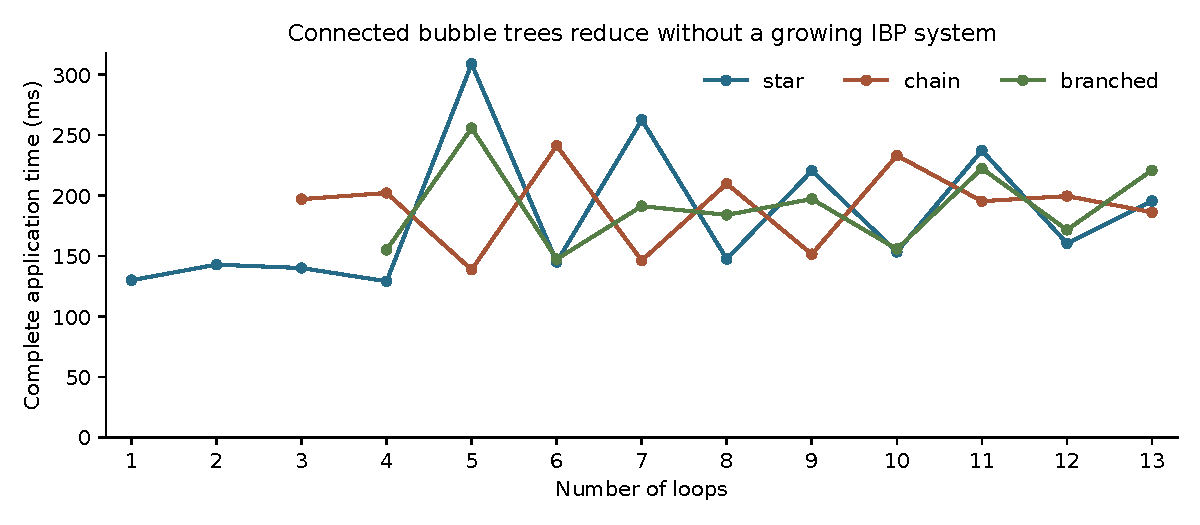
\includegraphics[width=\linewidth]{paper_figures/loop_coverage13_time.pdf}
\caption{The connected bubble-tree formula avoids a growing IBP system. Each point is the median complete application time for seven targets at the indicated loop count. The curves show rational-scale requests; the five symbolic requests enter the completion and check totals. Three repetitions measure process-level variation.}
\label{fig:notes-loop-tree-time}
\end{figure}
\begin{figure}[!htbp]\centering
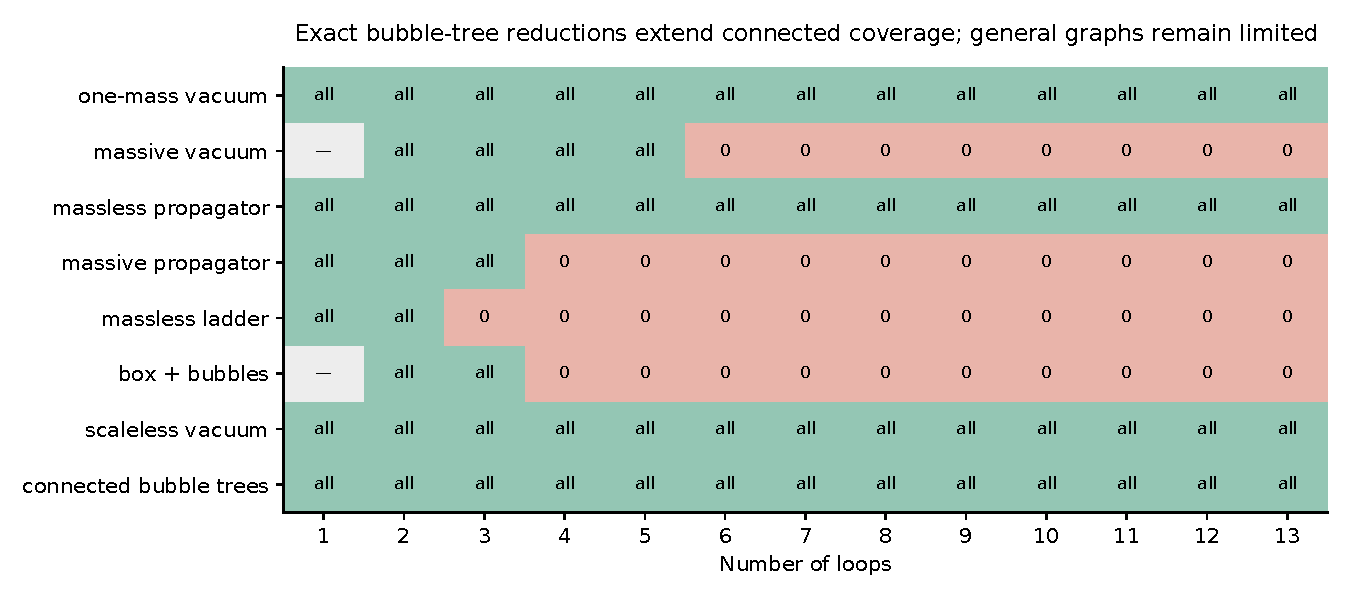
\includegraphics[width=\linewidth]{paper_figures/loop_coverage13.pdf}
\caption{Finite coverage at each loop order. ``All'' means that the method completed every request in that cell, and zero means none completed. A dash marks an omitted duplicate one-loop definition. The connected-tree row includes rational and symbolic requests; the other rows show the main rational grid. Additional scattering and symbolic cases remain included in Table~\ref{tab:notes-loop-tree-completion}. The figure describes these defined targets, not all integrals at that order.}
\label{fig:notes-loop-tree-coverage}
\end{figure}
\begin{table}[!htbp]\centering\small
\caption{Completion by loop order on the full broader grid and the added connected trees. Each entry gives completed requests divided by requested cases for the new method. The preceding-method column applies to the broader grid.}
\label{tab:notes-loop-tree-orders}
\begin{tabular}{@{}rrrr@{}}\toprule
Loops & Broader grid & Preceding grid & Connected trees\\\midrule
1 & 12/12 & 12/12 & 2/2 \\
2 & 12/12 & 12/12 & 2/2 \\
3 & 8/10 & 8/10 & 3/3 \\
4 & 4/7 & 4/7 & 3/3 \\
5 & 4/7 & 4/7 & 3/3 \\
6 & 5/10 & 5/10 & 4/4 \\
7 & 3/7 & 3/7 & 3/3 \\
8 & 3/7 & 3/7 & 3/3 \\
9 & 3/7 & 3/7 & 3/3 \\
10 & 3/7 & 3/7 & 3/3 \\
11 & 3/7 & 3/7 & 3/3 \\
12 & 3/7 & 3/7 & 3/3 \\
13 & 5/10 & 5/10 & 4/4 \\
\bottomrule\end{tabular}\end{table}

The broader grid completes 68 of 110 requests with the new method and 68 with the preceding application. The unresolved cases include general massive multi-loop integrals and multi-scale scattering structures that do not have the proved bubble-tree form. The input limits of the configured native path and application deadlines remain explicit outcomes. A complete scalar-product basis can exceed the index limit of that path even when an analytic subintegral formula remains valid. Thus loop count alone does not determine whether the reduction succeeds. The new result extends a connected analytic domain through thirteen loops; it does not establish acceleration for every integral type.
\FloatBarrier

\section{Connected bubble trees and their exact reduction}
\label{app:notes-loop-tree}
\subsection{Integral family and allowed powers}
We attach massless two-line subintegrals to a triangle with lightlike external momenta $p_1$ and $p_2$, where $p_1^2=p_2^2=0$ and $s=(p_1+p_2)^2\ne0$. Let $\mathcal T$ be a rooted tree with vertices $0,\ldots,L-1$, one loop momentum $\ell_j$ at each vertex, and parent $\pi(j)$ for every vertex $j\ne0$. A rooted tree has a unique path from each vertex to its root. The family is
\begin{equation}
 I_{\mathcal T}(\boldsymbol a,\boldsymbol v,b,c)=
 \int\prod_{j=0}^{L-1}\frac{d^d\ell_j}{i\pi^{d/2}}
 \frac{1}{(\ell_0^2)^{a_0}[(\ell_0-p_1)^2]^b
 [ (\ell_0-p_1-p_2)^2]^c}
 \prod_{j=1}^{L-1}
 \frac{1}{(\ell_j^2)^{a_j}[(\ell_j-\ell_{\pi(j)})^2]^{v_j}}.
 \label{eq:notes-loop-tree-family}
\end{equation}
Each denominator carries the Feynman prescription of the integral definition in these notes. We suppress it in this appendix to keep the equations readable. The vector $\boldsymbol a$ contains the powers $a_j$. The vector $\boldsymbol v$ contains the powers $v_j$ of the lines joining each nonroot vertex $j$ to its parent. The supported powers $a_j$, $v_j$, and $c$ are positive integers; $b$ is an integer and can describe a polynomial numerator. Auxiliary scalar-product coordinates have zero powers. The implementation checks these conditions and currently accepts at most thirteen loops and absolute powers at most sixteen. These implementation bounds are narrower than the derived meromorphic identity.

A star attaches every bubble directly to the root. A chain attaches vertex $j$ to $j-1$. The branched test attaches vertex $j$ to $\lfloor(j-1)/2\rfloor$. These denominators share loop momenta, so the integrals are connected rather than products of independent loop integrals. We choose $M_{\mathcal T}$ to be the integral with every physical power equal to one. The reduction below establishes a one-element basis for the stated powers in this family. It does not classify all subsectors or all possible numerator insertions.

\subsection{Integrating the two-line subintegral}
The method of integrating a massless two-line subgraph before further reduction is established in parametric propagator calculations~\cite{Ruijl2017Forcer}. We give the derivation needed for our vertex family. Use inverse propagators $-q^2-i0$ temporarily, and write $Q^2=-q^2-i0$. For loop momentum $k$, external momentum $q$, and propagator powers $u$ and $v$, define
\begin{equation}
 B(u,v;q)=\int\frac{d^d k}{i\pi^{d/2}}
 \frac{1}{[-k^2-i0]^u[-(k-q)^2-i0]^v}.
 \label{eq:notes-loop-tree-Bdef}
\end{equation}
Combining two inverse propagators $X$ and $Y$ with a Feynman parameter $x$ gives~\cite{Weinzierl2022}
\begin{equation}
 \frac{1}{X^uY^v}=\frac{\Gamma(u+v)}{\Gamma(u)\Gamma(v)}
 \int_0^1 dx\,\frac{x^{u-1}(1-x)^{v-1}}
 {[xX+(1-x)Y]^{u+v}}.
 \label{eq:notes-loop-tree-param}
\end{equation}
After shifting the loop momentum and carrying out its integral, the remaining parameter integral is a beta integral:
\begin{align}
 B(u,v;q)&=(Q^2)^{d/2-u-v}
 \frac{\Gamma(u+v-d/2)}{\Gamma(u)\Gamma(v)}
 \int_0^1 dx\,x^{d/2-v-1}(1-x)^{d/2-u-1}\notag\\
 &=(Q^2)^{d/2-u-v}G(u,v),\label{eq:notes-loop-tree-bubble}\\
 G(u,v)&=\frac{\Gamma(u+v-d/2)\Gamma(d/2-u)\Gamma(d/2-v)}
 {\Gamma(u)\Gamma(v)\Gamma(d-u-v)}.\label{eq:notes-loop-tree-G}
\end{align}
The parameter representation first holds in a convergence domain and then defines the dimensionally regularized expression by meromorphic continuation~\cite{Weinzierl2022}. Removing a leaf therefore transfers the power $u+v-d/2$ to its parent's squared momentum.

Let $\mathcal C(j)$ be the children of vertex $j$. Starting from the leaves, define the effective squared-momentum power $u_j$ and transferred power $\sigma_j$ by
\begin{equation}
 u_j=a_j+\sum_{h\in\mathcal C(j)}\sigma_h,
 \qquad \sigma_j=u_j+v_j-\frac d2\quad(j\ne0),
 \qquad \alpha=a_0+\sum_{h\in\mathcal C(0)}\sigma_h.
 \label{eq:notes-loop-tree-transfer}
\end{equation}
Each integration contributes $G(u_j,v_j)$. The remaining triangle has powers $(\alpha,b,c)$. Its first power is generally noninteger, which is why simply treating the contracted line as an ordinary integer-index Kira input would be insufficient.

\subsection{Integrating the remaining triangle}
For $A=\alpha+b+c$ and $S=-s-i0$, the triangle parameter representation in the same inverse-propagator convention is
\begin{align}
 \widetilde T(\alpha,b,c)
 &=\frac{\Gamma(A-d/2)S^{d/2-A}}
 {\Gamma(\alpha)\Gamma(b)\Gamma(c)}
 \int_{x_i\ge0}dx_1dx_2dx_3\,
 \delta(1-x_1-x_2-x_3)\notag\\[-2pt]
 &\hspace{20mm}\times x_1^{d/2-b-c-1}x_2^{b-1}
 x_3^{d/2-\alpha-b-1}\notag\\
 &=S^{d/2-A}H(\alpha,b,c),\label{eq:notes-loop-tree-triangle}\\
 H(\alpha,b,c)
 &=\frac{\Gamma(A-d/2)\Gamma(d/2-\alpha-b)\Gamma(d/2-b-c)}
 {\Gamma(\alpha)\Gamma(c)\Gamma(d-A)}.
 \label{eq:notes-loop-tree-H}
\end{align}
The Dirichlet integral in the first expression produces a factor $\Gamma(b)$ that cancels its prefactor. This cancellation gives the continuation to zero and negative integer $b$. The formula extends the one-loop parameter derivation in Appendix~\ref{app:notes-analytic-batch} to the shifted power $\alpha$ generated by connected bubbles.

Let $A_{\rm tot}=a_0+b+c+\sum_{j\ne0}(a_j+v_j)$ be the sum of all physical powers and define
\begin{equation}
 \mathcal C_{\mathcal T}(\boldsymbol a,\boldsymbol v,b,c)
 =H(\alpha,b,c)\prod_{j\ne0}G(u_j,v_j).
 \label{eq:notes-loop-tree-C}
\end{equation}
Equations~\eqref{eq:notes-loop-tree-transfer}--\eqref{eq:notes-loop-tree-H} give the scale power $S^{Ld/2-A_{\rm tot}}$, as required directly by dimensional counting. If $\Delta=A_{\rm tot}-(2L+1)$, division by the unit-power integral cancels the common scale dependence. Returning to the original $q^2+i0$ convention contributes $(-1)^\Delta$, and $(-1)^\Delta(-s)^{-\Delta}=s^{-\Delta}$ for integer $\Delta$. Thus
\begin{equation}
 I_{\mathcal T}(\boldsymbol a,\boldsymbol v,b,c)=
 s^{-\Delta}\frac{\mathcal C_{\mathcal T}(\boldsymbol a,\boldsymbol v,b,c)}
 {\mathcal C_{\mathcal T}(\boldsymbol 1,\boldsymbol 1,1,1)}M_{\mathcal T}.
 \label{eq:notes-loop-tree-reduction}
\end{equation}
The equality holds as a meromorphic identity for generic dimension and nonzero scale, with the continuation fixed by the original Feynman prescription.

\subsection{Obtaining rational coefficients}
Every Gamma argument has the form $z=A+Bd/2$ with integer $A$ and $B$. Changing integer propagator powers changes $A$ while leaving $B$ fixed for the same tree. Repeated use of $\Gamma(z+1)=z\Gamma(z)$ therefore yields
\begin{equation}
 \frac{\Gamma(z+n)}{\Gamma(z)}=
 \begin{cases}
 \prod_{r=0}^{n-1}(z+r),&n\ge0,\\
 \displaystyle\left[\prod_{r=1}^{-n}(z-r)\right]^{-1},&n<0.
 \end{cases}
 \label{eq:notes-loop-tree-shift}
\end{equation}
The empty product is one. Applying this identity to Eq.~\eqref{eq:notes-loop-tree-reduction} proves that its coefficient lies in $\Q(d,s)$. We cancel common linear factors before expanding any polynomial. This preserves exactness while avoiding large intermediate expressions. Neither a learned coefficient nor a numerical Gamma evaluation enters the deployed reduction.

A longest path from the root terminates at a vertex without children. Equation~\eqref{eq:notes-loop-tree-bubble} removes this leaf and leaves a tree with one fewer loop and a shifted parent power. The Gamma formula permits that noninteger power. Repeating this step reaches the one-loop triangle, which Eq.~\eqref{eq:notes-loop-tree-triangle} evaluates. This induction proves the reduction for every finite rooted tree that satisfies the stated physical assumptions. The numerical tests below cover a finite set of such trees through thirteen loops. They do not extend this proof to massive insertions, general auxiliary numerators, or multi-scale root graphs.

\subsection{The reserved connected targets}
All powers start at one and all auxiliary powers are zero. Each connected request contains the following seven assignments: the unchanged unit powers; $a_0=2$; $b=0$; $b=-1$; $c=3$; $v_{L-1}=2$ for $L>1$ (or $c=2$ for $L=1$); and the combined assignment $a_0=b=2$, $c=1$, $a_j=1$, $v_j=2$ for every $j\ne0$. An assignment changes only the stated powers. The rational-scale requests use $s=-6296$ in a common squared-momentum unit, and the symbolic requests retain $s$ as a nonzero variable. The tree definitions above specify every physical denominator. Complete independent scalar-product coordinates fill the remaining zero-power positions.

\subsection{Matched application times and request variation}
For each completed request $i$, let $t_{i,\mathrm{new}}$ and $t_{i,\mathrm{control}}$ be the medians of its three application times. The time ratio divides their sums over the same matched requests, so subtracting this ratio from one gives the fractional saving. To describe variation among requests, we draw $n$ matched request indices $i_1,\ldots,i_n$ with replacement from a collection of size $n$ and calculate
\begin{equation}
 R^*=\frac{\sum_{r=1}^{n}t_{i_r,\mathrm{new}}}
 {\sum_{r=1}^{n}t_{i_r,\mathrm{control}}}.
 \label{eq:notes-loop-tree-resampling}
\end{equation}
This applies the bootstrap construction~\cite{Efron1979} to complete paired requests. We retain the central 95\% of 2,000 resampled ratios. The interval describes the finite request collection; it is not a guarantee for new physical graph classes. This request resampling differs from the paired repetition resampling used in the earlier native comparisons.

% END CURRENT WORKFLOW UPDATE
% BEGIN CURRENT WORKFLOW UPDATE
\section{Cancelling common factors before expansion}
\label{sec:notes-gamma-cancel}
The connected identity removes the need to generate an IBP system for the supported trees, but a large target batch still requires many rational coefficients. The preceding implementation expands integer shifts of individual Gamma ratios and then cancels their common linear factors. We instead collect and cancel complete Gamma factors across the full integral before producing any finite products. We also calculate the dimension-dependent part of each subintegral power and the reference-master arguments once per batch. Appendix~\ref{app:notes-gamma-cancel} derives these steps from the same bubble and triangle identities.

For each common dimension coefficient $B$, the method combines the signed multiplicities of $\Gamma(A+Bd/2)$. Their sum vanishes in the target-to-master ratio. The finite-product identity in Appendix~\ref{app:notes-gamma-cancel} then produces only intervals with nonzero net multiplicity. This avoids forming factors that would cancel later. Integer arithmetic keeps the result exact. The method uses the same master and physical domain as the preceding connected reduction, while other integrals retain the existing exact and learned Kira workflow.

We compare 34 distinct tree structures through thirteen loops, with a small and a large symbolic-scale batch for each structure. The small batch contains seven targets. The large batch contains 128 targets with physical powers up to four, except at one loop, where its full allowed set has 96 targets. Four further requests check the unchanged analytic and native paths. Each method runs five times in a fresh process, with rotated order and the same output procedure. The timer includes loading, recognition, coefficient calculation, output, and exit. Independent comparisons occur after timing. The control uses the preceding coefficient routine in the same application, which isolates the combined effect of early mathematical cancellation and shared batch calculations.

All 72 requests complete in every repetition. The 4,558 connected target entries agree exactly with the preceding canonical rational coefficients, and 612 independent Gamma evaluations pass at 80-digit precision with relative tolerance $10^{-60}$. The Gamma checks use three selected targets from each connected request at the three dimensions defined in Appendix~\ref{app:notes-loop-tree}. They test the implementation of the proved identity and do not constitute new native high-loop reductions.

\begin{table}[!htbp]\centering\small
\caption{Complete application times for the cancellation comparison. Each total sums request medians from five repetitions. The interval resamples complete requests. A ratio below one denotes less time.}
\label{tab:notes-gamma-cancel}
\begin{tabularx}{\linewidth}{@{}Yrrrr@{}}\toprule
Collection & Requests & Previous (s) & New (s) & Ratio\\\midrule
Large batches & 34 & 14.305 & 6.731 & 0.471 \\
Seven-target batches & 34 & 4.838 & 4.964 & 1.026 \\
Unchanged-path checks & 4 & 4.412 & 4.404 & 0.998 \\
All requests & 72 & 23.556 & 16.100 & 0.683 \\
\bottomrule\end{tabularx}\end{table}

For the large connected batches, the new method uses 52.9\% less total time, with ratio 0.471 and request-resampling interval $[0.414,0.540]$. All 34 large requests have a shorter median time. The seven-target ratio is 1.026, with request-resampling interval $[0.986,1.071]$ and 17 slower requests. These short calls include loading and output, so a faster coefficient calculation need not produce a proportional saving in complete time. Across all 68 connected requests, time falls from 19.143 to 11.695 seconds. Including the four unchanged-path checks, total time falls from 23.556 to 16.100 seconds, or 31.7\% less time on this 72-request collection. The small-batch interval includes equal time, so the comparison does not resolve an improvement for short calls. These savings arise from exact simplification and shared calculation within a batch. The trained native choices remain unchanged, so this comparison does not assign the added gain to ML. It also preserves the preceding coverage limits for massive and multi-scale graphs.

\begin{figure}[!htbp]\centering
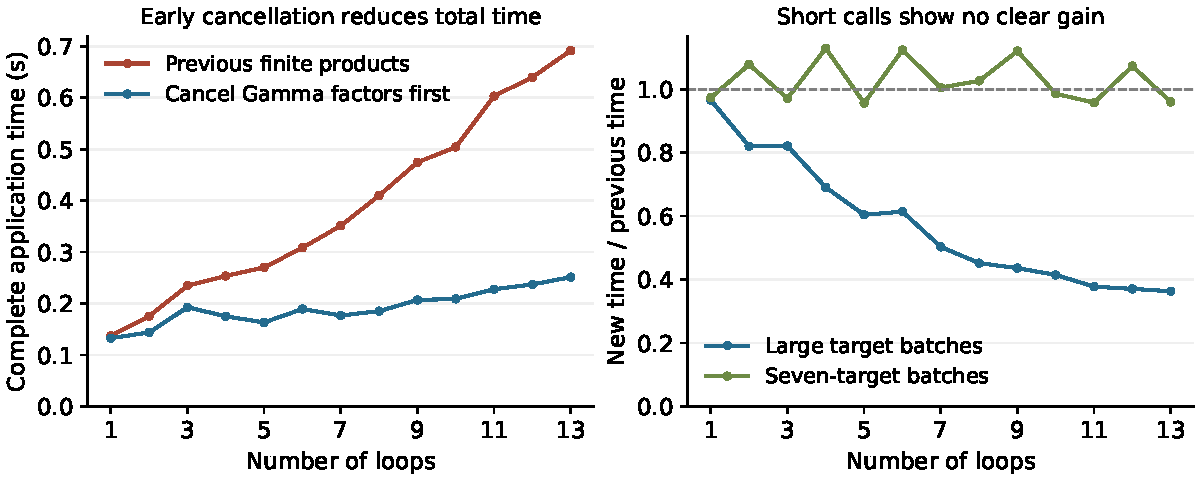
\includegraphics[width=\linewidth]{paper_figures/gamma_cancellation.pdf}
\caption{Early cancellation reduces complete time as the coefficient algebra grows. The left panel averages large-batch request medians at each loop order. The right panel divides summed new medians by summed control medians separately for each batch size. The one-loop large batch has 96 targets; the other large batches have 128. Each point compares matching structures and targets.}
\label{fig:notes-gamma-cancel}
\end{figure}
\FloatBarrier

\section{Cancellation of Gamma factors before finite expansion}
\label{app:notes-gamma-cancel}
The connected reduction in Appendix~\ref{app:notes-loop-tree} expresses the coefficient as a ratio of products of Gamma functions. Every argument has the form $A+Bd/2$, where $A$ and $B$ are integers. The tree fixes $B$, while the target powers determine $A$. We first explain how to reuse this fixed part and then derive the cancellation rule.

Let $n_j$ be the number of vertices in the subtree rooted at a nonroot vertex $j$, including $j$ itself. Write the integer part of its incoming effective power as $U_j$. The definitions in Eq.~\eqref{eq:notes-loop-tree-transfer} give
\begin{equation}
 u_j=U_j-(n_j-1)\frac d2,
 \qquad U_j=a_j+\sum_{h\in\mathcal C(j)}(U_h+v_h),
 \qquad \sigma_j=U_j+v_j-n_j\frac d2.
 \label{eq:notes-gamma-cancel-subtree}
\end{equation}
For a leaf, $n_j=1$ and $U_j=a_j$, so this expression agrees with the one-bubble formula. If it holds for the children, summing their transferred powers gives the expression at their parent because $n_j=1+\sum_h n_h$. Induction therefore proves the formula throughout the tree. The subtree sizes can be calculated once for a batch of targets. At the root, define $U_0=a_0+\sum_{h\in\mathcal C(0)}(U_h+v_h)$, so the corresponding power is $\alpha=U_0-(L-1)d/2$.

Substitution in the bubble factor gives numerator arguments
\begin{equation}
 U_j+v_j-n_jd/2,\qquad -U_j+n_jd/2,\qquad -v_j+d/2,
\end{equation}
and denominator arguments
\begin{equation}
 U_j+(1-n_j)d/2,\qquad v_j,\qquad -U_j-v_j+(n_j+1)d/2.
\end{equation}
The root-triangle arguments follow by substituting $\alpha$ into Eq.~\eqref{eq:notes-loop-tree-H}. These expressions evaluate the same Gamma arguments as the preceding recursive method and avoid calculating their dimension-dependent parts separately for each target.

After dividing by the unit-power master, collect the factors with a fixed value of $B$. Cancel identical arguments and order the remaining integer parts as $A_1<\cdots<A_m$. Let $w_i$ be the signed multiplicity of $\Gamma(A_i+Bd/2)$, with numerator factors positive. The target and master have matching argument slopes, so $\sum_i w_i=0$. Define $C_i=\sum_{j=1}^i w_j$. Then
\begin{equation}
 \prod_{i=1}^{m}\Gamma(A_i+Bd/2)^{w_i}
 =\prod_{i=1}^{m-1}\prod_{k=A_i}^{A_{i+1}-1}
       (k+Bd/2)^{-C_i}.
 \label{eq:notes-gamma-cancel-product}
\end{equation}
To prove this identity, use Eq.~\eqref{eq:notes-loop-tree-shift} to write every Gamma function relative to $\Gamma(A_1+Bd/2)$. Its total exponent is zero. A factor in the interval from $A_i$ to $A_{i+1}-1$ appears in precisely the terms with index greater than $i$, so its exponent is $\sum_{j>i}w_j=-C_i$. This gives Eq.~\eqref{eq:notes-gamma-cancel-product}. Intervals with $C_i=0$ contribute one and require no factors. The identity holds meromorphically under the same physical assumptions as the connected reduction.

Finally, we normalize each linear factor by the integer greatest common divisor of its two coefficients and combine equal normalized factors. Integer numerator and denominator products accumulate separately, and one rational simplification reduces their ratio. We compute the reference-master arguments once per target batch. These changes preserve the exact coefficient and master basis.

The reserved comparison uses the distinct star, chain, and branched structures defined in Appendix~\ref{app:notes-loop-tree}, giving 34 structures through thirteen loops. For each structure, the small batch uses the seven stated target assignments. The large batch includes those assignments and additional distinct powers: every positive physical power lies between one and four, and the middle triangle power lies between minus one and four. Auxiliary powers remain zero. The scale $s$ stays symbolic. Each large batch has 128 targets except at one loop, where the allowed set contains 96 targets. The selected finite sets are recorded with the results; the analytic formula applies throughout the stated domain.

Five fresh processes measure each method on each request. The comparison rotates method order and uses the same input, output procedure, machine, and master basis. The ratio divides sums of request medians, with request-resampling intervals defined in Eq.~\eqref{eq:notes-loop-tree-resampling}. Loading, recognition, coefficient calculation, output, and process exit enter the timer. Exact comparison with the preceding coefficient routine and independent Gamma evaluations occur after timing and are excluded for both methods. The four regression requests exercise two earlier analytic families at thirteen loops and planar and nonplanar two-loop native batches. They test the unchanged fallback path and do not provide a new estimate of the separate ML contribution.

% END CURRENT WORKFLOW UPDATE
% BEGIN CURRENT WORKFLOW UPDATE
\section{Connected two-point reductions and the native index limit}
\label{sec:notes-prop-tree}
The preceding triangle identity suggests a further reduction: a connected tree of massless bubbles also closes analytically when its root is a two-point integral. We implement this extension before the existing analytic and learned choices. It recognizes the momenta, masses, and powers, integrates each nonroot bubble, and evaluates the remaining root bubble. The dimension-dependent powers transferred between subintegrals are retained exactly. Appendix~\ref{app:notes-prop-tree} defines the family and derives the rational target-to-master coefficient. This use of massless subintegrals follows established parametric propagator methods~\cite{Ruijl2017Forcer}.

This extension also clarifies the apparent loop limit. Kira requires a complete set of $N=L(L+1)/2+LE$ scalar-product coordinates for $L$ loops and $E$ independent external momenta~\cite{Kira3}. The installed native build rejects more than 31 indices, including auxiliary scalar-product coordinates. Consequently, its complete-coordinate limit is seven loops for vacuum families, six for two-point families, and five for families with two or three independent external momenta. Appendix~\ref{app:notes-prop-tree} derives the coordinate count. Exact integration bypasses this native input within the stated analytic domain; it does not remove the restriction for an arbitrary remaining graph.

We freeze 34 distinct two-point tree structures with seven targets each, covering every loop order from one through thirteen. Their scale remains symbolic. Three fresh processes compare the extended application with the preceding application under a twelve-second limit per call. Sixteen triangle requests check the unchanged exact path, while sixteen native two-loop box requests also compare the retained trained choices with fixed choices. The complete timer includes startup, recognition, coefficient calculation or native reduction, model evaluation when used, output, and exit. Independent checks follow timing on both sides.

All 34 two-point requests complete with the new rule. The preceding application completes 3 in every repetition. Among its 31 unsuccessful requests, 21 exceed the native index limit, nine reach the application deadline, and one fails the master-basis verification. We retain these failures in the completion counts and calculate speed ratios only from matched completed requests. The reserved two-point targets pass 714 independent Gamma checks at 80-digit precision and scaled error tolerance $10^{-60}$. Development also supplies 9 exact coefficient comparisons with native Kira. These checks test the derived identity; the high-loop results do not represent native high-loop IBP solves.

\begin{table}[!htbp]\centering\small
\caption{Complete times from sums of three-run request medians. The completion columns count requests completed in all repetitions. Times use only requests completed by both methods. The ML row uses fixed native choices as its control.}
\label{tab:notes-prop-tree}
\begin{tabularx}{\linewidth}{@{}Yrrrr@{}}\toprule
Comparison & Control/new complete & Paired & Control (s) & New (s)\\\midrule
Two-point trees & 3/34 & 3 & 11.185 & 0.433 \\
Triangle checks & 16/16 & 16 & 2.557 & 2.593 \\
Native path checks & 16/16 & 16 & 48.719 & 48.941 \\
Retained ML versus fixed & 16/16 & 16 & 52.226 & 48.941 \\
\bottomrule\end{tabularx}\end{table}

For the 3 matched two-point requests, total time falls from 11.185 to 0.433 seconds, a reduction of 96.1\%. The time ratio is 0.039, with a request-resampling interval of $[0.015,0.859]$. Across all 35 matched requests in this comparison, time changes from 62.461 to 51.967 seconds. The analytic extension accounts for the new two-point gain. No new ML model is fitted for this identity.

The matched collection-wide ratio is 0.832, with request interval $[0.569,1.010]$. This interval includes equal time, so the collection-wide point estimate does not establish a gain across integral families. The unchanged triangle and native paths also have intervals that include equal time.

On the sixteen native requests, the retained learned choices take 48.941 seconds against 52.226 seconds for fixed choices, giving ratio 0.937 and request-resampling interval $[0.853,1.010]$. The trained batch policy runs on all sixteen requests, choosing the wider sparse seed setting thirteen times and the tighter setting three times. This fresh comparison does not resolve a reliable ML gain because the interval includes equal time. The earlier controlled seed and equation-selection gains remain separate evidence. The new two-point reduction retains the preceding ML policy for its eligible native inputs. It supports the specified connected massless trees and preserves the documented failures for general massive, multiscale, and irreducible scattering families.

\begin{figure}[!htbp]\centering
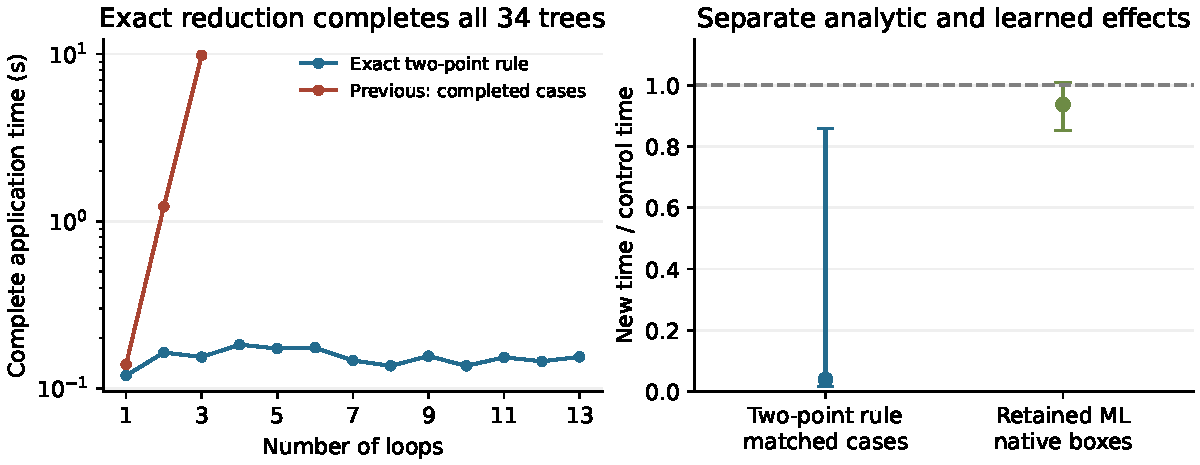
\includegraphics[width=\linewidth]{paper_figures/propagator_trees.pdf}
\caption{The exact rule completes the defined two-point trees through thirteen loops. The left panel uses a logarithmic time axis and averages request medians at each loop order. Control points include completed requests only; missing points have no completed control and imply no finite speed factor. The right panel separates the exact extension from the retained native ML contribution, using matched completed requests and request-resampling intervals.}
\label{fig:notes-prop-tree}
\end{figure}
\FloatBarrier

\section{Exact reduction of connected two-point trees}
\label{app:notes-prop-tree}
\subsection{Family and analytic reduction}
The bubble integral in Eq.~\eqref{eq:notes-loop-tree-G} also closes a two-point graph when every nonroot vertex is a massless bubble. Such subintegral integration is used in parametric propagator calculations~\cite{Ruijl2017Forcer}. We derive the precise family needed here. Let $\mathcal T$ be a rooted tree with $L$ vertices, root $0$, and parent $\pi(j)$ for each $j\ne0$. Each vertex has loop momentum $\ell_j$. The external momentum $p$ obeys $p^2=s\ne0$. Define
\begin{equation}
 J_{\mathcal T}(\boldsymbol a,\boldsymbol v,c)=
 \int\prod_{j=0}^{L-1}\frac{d^d\ell_j}{i\pi^{d/2}}
 \frac{1}{(\ell_0^2)^{a_0}[(\ell_0-p)^2]^c}
 \prod_{j=1}^{L-1}
 \frac{1}{(\ell_j^2)^{a_j}[(\ell_j-\ell_{\pi(j)})^2]^{v_j}}.
 \label{eq:notes-prop-tree-family}
\end{equation}
The Feynman prescription is implicit, as in Appendix~\ref{app:notes-loop-tree}. All internal masses vanish. The vectors $\boldsymbol a$ and $\boldsymbol v$ contain the integer powers on the squared loop momenta and connecting lines. The power $c$ belongs to the external root line. The connecting powers $v_j$, the external root power $c$, and each leaf power $a_j$ must be positive integers. At a vertex with children, $a_j$ may also be zero or negative: the already integrated children supply a dimension-dependent effective power. The implementation accepts zero auxiliary powers, at most thirteen loops, and absolute powers at most sixteen. Define $M_{\mathcal T}$ by setting every physical power to one. The following argument establishes a one-element basis within this domain and does not classify all subsectors or irreducible numerators.

For each nonroot vertex, define its effective power and the power transferred to its parent by
\begin{equation}
 u_j=a_j+\sum_{h\in\mathcal C(j)}\sigma_h,
 \qquad \sigma_j=u_j+v_j-\frac d2,
 \qquad \alpha=a_0+\sum_{h\in\mathcal C(0)}\sigma_h,
 \label{eq:notes-prop-tree-transfer}
\end{equation}
where $\mathcal C(j)$ is the set of children of vertex $j$. A leaf has $u_j=a_j$. Its integration gives $G(u_j,v_j)$ and a factor $(\ell_{\pi(j)}^2)^{-\sigma_j}$ in the temporary negative-propagator convention used in Appendix~\ref{app:notes-loop-tree}. Repeating this operation removes every nonroot vertex. The remaining root integral is the same bubble formula with powers $(\alpha,c)$. Thus its dimensionless coefficient is
\begin{equation}
 C_{\mathcal T}(\boldsymbol a,\boldsymbol v,c;d)
 =G(\alpha,c)\prod_{j=1}^{L-1}G(u_j,v_j).
 \label{eq:notes-prop-tree-Gproduct}
\end{equation}
The one-loop derivation of $G$ appears in Eqs.~\eqref{eq:notes-loop-tree-param}--\eqref{eq:notes-loop-tree-G}, so induction on the number of vertices proves Eq.~\eqref{eq:notes-prop-tree-Gproduct}. It first holds in a convergence domain and then extends meromorphically in $d$ and the powers~\cite{Weinzierl2022}.

Let $A=\sum_{j=0}^{L-1}a_j+\sum_{j=1}^{L-1}v_j+c$ be the sum of physical powers. Summing the transferred powers in Eq.~\eqref{eq:notes-prop-tree-transfer} gives $\alpha+c=A-(L-1)d/2$. The last bubble therefore contributes the scale power $(-s-i0)^{Ld/2-A}$. The unit-power master has $A_0=2L$, because the root and each nonroot vertex supply two physical lines. Dividing the target expression by the master expression cancels the common noninteger scale power. Restoring the positive-propagator convention gives
\begin{equation}
 J_{\mathcal T}(\boldsymbol a,\boldsymbol v,c)
 =s^{-\Delta}\,
 \frac{C_{\mathcal T}(\boldsymbol a,\boldsymbol v,c;d)}
 {C_{\mathcal T}(\boldsymbol 1,\boldsymbol 1,1;d)}
 M_{\mathcal T},
 \qquad \Delta=A-2L.
 \label{eq:notes-prop-tree-reduction}
\end{equation}
Indeed, the target-to-master change of propagator convention contributes $(-1)^\Delta$, which cancels the sign in $(-s)^{-\Delta}$ for integer $\Delta$. The relation therefore uses the same convention as the native reductions.

Every effective power has an integer part and a fixed integer coefficient of $d/2$. For a subtree with $n_j$ vertices, $u_j=U_j-(n_j-1)d/2$, with $U_j=a_j+\sum_{h\in\mathcal C(j)}(U_h+v_h)$, as proved in Appendix~\ref{app:notes-gamma-cancel}. At the root, $\alpha=U_0-(L-1)d/2$. The target and master therefore have matching Gamma-argument slopes and integer argument differences. Equation~\eqref{eq:notes-gamma-cancel-product} converts their ratio to finite products of linear factors in $d$. This proves that the coefficient in Eq.~\eqref{eq:notes-prop-tree-reduction} lies in $\mathbb Q(d,s)$. The calculation cancels equal Gamma factors before expanding those products and shares the subtree sizes and master arguments across the target batch.

\subsection{Loop count and the native input restriction}
For $L$ independent loop momenta, the loop--loop scalar products consist of $L$ squares and $L(L-1)/2$ distinct mixed products. Each of the $E$ independent external momenta adds $L$ loop--external products. Their sum is
\begin{equation}
 N=L+\frac{L(L-1)}2+LE=\frac{L(L+1)}2+LE,
 \label{eq:notes-prop-tree-index-count}
\end{equation}
which is the complete-coordinate count used by Kira~\cite{Kira3}. The native build used in this study rejects $N>31$. This measured implementation restriction gives different loop limits for different values of $E$. It permits complete coordinates through seven loops for $E=0$, six for $E=1$, and five for $E=2$ or $E=3$. It does not define a general seven-loop boundary for IBP identities. Equation~\eqref{eq:notes-prop-tree-reduction} avoids that native input for its stated domain, while unrecognized families retain the native restriction.

\subsection{Checks and time comparison}
We use stars, chains, and trees with parent $\pi(j)=\lfloor(j-1)/2\rfloor$. We retain one representative at one and two loops, two at three loops, and three at each higher order, giving 34 two-point structures through thirteen loops. Each request has seven distinct target assignments, including the unit master, single raised powers, and further positive powers between one and three. All auxiliary powers vanish and $s$ remains symbolic. Development targets and the reserved timing targets use separate fixed assignments.

Section~\ref{sec:notes-prop-tree} defines the complete application timer, three repetitions, unchanged-path checks, and native ML control. Failed controls remain in the completion counts. Speed ratios use matched completed requests, with request-resampling intervals defined in Eq.~\eqref{eq:notes-loop-tree-resampling}.

For each two-point target, independent full Gamma products test the coefficient at 80-digit precision and $d=137/101$, $151/103$, and $163/107$, with scaled error below $10^{-60}$. We use $e=|c_{\mathrm{num}}-c_\Gamma|/\max(1,|c_\Gamma|)$, where $c_{\mathrm{num}}$ evaluates the returned coefficient and $c_\Gamma$ evaluates the full Gamma product. These checks test the derived identity within its stated domain.

% END CURRENT WORKFLOW UPDATE
% BEGIN CURRENT WORKFLOW UPDATE
\section{Exact massive vacuum reduction and retrained seed choices}
\label{sec:notes-vac-ml}
The two-point reduction can also close when the tree ends at a massive vacuum line. We add this identity to cover connected vacuum integrals with one massive root denominator and massless bubble branches. Each branch changes the power of the root momentum, and a beta integral then evaluates the root. Appendix~\ref{app:notes-vac-ml} defines the family and derives its rational coefficient relative to the unit-power master. This calculation uses the same subintegral principle as parametric massless reduction~\cite{Ruijl2017Forcer}, with the massive root derived explicitly here. The application checks the momenta, masses, and index powers before applying the identity, applies the rule within independent loop blocks when present, and retains the existing exact rules and Kira choices for other inputs.

For integrals that still require Kira, we train a new model to choose the sparse seed boundary before equation generation. Kira already supplies optimized seeding and equation selection~\cite{Kira3}; the learned decision chooses among three boundaries in the existing exact reduction interface. The wider and tighter boundaries come from the preceding implementation, and a third boundary gives an intermediate seed region. Appendix~\ref{app:notes-vac-ml} derives the training objective. The seed-boundary parameters use the definition in Appendix~\ref{app:seed-geometry}:
\begin{equation}
 \begin{split}
 \boldsymbol\theta_{\mathrm{wide}}&=(2.5,0,0,1.25,0,1,-0.25),\\
 \boldsymbol\theta_{\mathrm{tight}}&=(1,0,0,0,1,1,0),\\
 \boldsymbol\theta_{\mathrm{middle}}&=(1.5,0,0,0.5,0,1,0).
 \end{split}
 \label{eq:notes-vac-ml-choices}
\end{equation}
These are specified candidate settings rather than physical identities. All candidates use the same protected master basis, native truncation setting, exact checks, and recovery mechanism.

The model uses 25 input features. They describe loop and external-momentum counts, propagator incidence, target count, numerator ranks, positive powers, and distances between target index vectors. The added features describe the minimum, maximum, and mean power of each of the two auxiliary denominators and the fraction of targets with zero power in each. No family name or known reduction coefficient enters the prediction. We collect complete timings for 32 training requests and 16 validation requests from planar and nonplanar massless two-loop boxes, whose propagators are defined in Appendix~\ref{app:families}. Their numerator ranks range from one to four, and all seven physical denominators have unit power. Each batch contains one to four targets. The sets of numerator-power pairs that define the batches are disjoint across training, validation, and the 32 reserved native requests; individual pairs can occur in different batches. Each split also uses different rational kinematics. These are new target batches within two known topology classes, so they do not establish transfer to unseen graph classes. The eligibility gate checks counts, masses, powers, and feature ranges; it does not certify that an arbitrary graph belongs to the training classes. Native basis checks and recovery retain responsibility for algebraic completion.

Candidate models contain one cost tree or an ensemble of 24 trees, using tree and bootstrap-ensemble methods~\cite{CART1984,Breiman2001Forest} with the time objective derived here. Each ensemble tree draws 32 training requests with replacement and considers a random set of 12 of the 25 features at each split. Leaves store the mean measured cost of each action, and the ensemble averages these costs. Validation compares depths one through four, minimum leaf sizes two, four, or eight, and predicted-saving margins of zero, three, eight, or fifteen percent. We enable the selected policy only if it changes at least one validation choice, adds no unverified result, and improves the fixed validation cost by at least one percent after the prediction allowance.

Validation selects 24 tree(s), maximum depth 3, minimum leaf size 2, and predicted-saving margin 0\%. The fixed comparison uses the tighter boundary, which has the lowest total validation time. The learned policy is enabled by the validation criterion. Its selected validation cost, including a two-millisecond prediction allowance per request, is 71.673 seconds, compared with 76.165 seconds for the fixed choice. These validation values select the policy and do not serve as its independent result.

We freeze the policy and implementation before testing. The exact test contains 34 distinct rooted vacuum structures, with seven targets each and a symbolic mass scale, covering every loop order from one through thirteen. Eight additional requests check the retained two-point and triangle rules. Each reserved request runs three times in fresh processes, with method order rotated and an eighteen-second application limit. The timer includes process loading, input, recognition, model loading and inference when used, native algebra and recovery, output, and exit. Direct analytic requests defer native and model imports until they are needed. Independent comparisons of returned coefficients run outside both timers. Native comparisons use the same previously verified master-index information; reference preparation is excluded equally. The previous-method comparison launches the preceding published application directly. We draw 2,000 resamples of matched requests with replacement, retain each request's paired medians, and take the 2.5 and 97.5 percentiles of the time ratios. These intervals describe variation within the finite request collection.

The new rule completes 34 of 34 vacuum requests in every repetition, while the preceding application completes 4. The reserved vacuum coefficients pass 714 independent Gamma evaluations at 80-digit precision, with scaled error below $10^{-60}$. The scaled error is the absolute difference divided by the larger of one and the reference magnitude. Separate development checks supply 9 exact coefficient comparisons with native Kira.

Before the reserved comparison, six transformation checks preserve the coefficients under loop renaming, common momentum-sign reversal, and physical-denominator reordering. Three product checks verify the integrated rule on independent vacuum blocks with four, eight, and thirteen total loops. These product checks establish composition of the supported identity and supply no separate timing claim.

\begin{table}[!htbp]\centering\small
\caption{Sums of three-run median complete times. Times use requests completed and verified by both methods. Completion counts retain all requests and require all repetitions to pass.}
\label{tab:notes-vac-ml}
\begin{tabularx}{\linewidth}{@{}Yrrrr@{}}\toprule
Comparison & Control/new complete & Paired & Control (s) & New (s)\\\midrule
Vacuum trees versus previous & 4/34 & 4 & 5.046 & 0.730 \\
Native application versus previous & 31/32 & 31 & 186.074 & 139.678 \\
Native model versus fixed & 32/32 & 32 & 156.383 & 150.663 \\
Two-point regression checks & 4/4 & 4 & 0.626 & 0.686 \\
Triangle regression checks & 4/4 & 4 & 0.648 & 0.792 \\
\bottomrule\end{tabularx}\end{table}

The matched vacuum comparison gives time ratio 0.145, with a central 95\% request-resampling interval of $[0.096,0.379]$. The new method takes longer on 0 of the 4 matched requests.

The revised native application against the preceding application gives time ratio 0.751, with a central 95\% request-resampling interval of $[0.675,0.841]$. The new method takes longer on 10 of the 31 matched requests.

The new native model against fixed choices gives time ratio 0.963, with a central 95\% request-resampling interval of $[0.937,0.984]$. The new method takes longer on 10 of the 32 matched requests.

The final-repetition audit of the 32 matched native requests records 2 unsuccessful internal attempts with the learned choices and 14 with the fixed choice. The corresponding sums of logged equation-generation counts are 286,531 and 326,825; these count regenerated rows as further equation instances. Thus the audit distinguishes failed internal attempts that later recover from requests that never complete. The complete-time comparison includes both kinds of cost.

For the planar boxes alone, the learned-to-fixed ratio is 0.929, with request interval $[0.870,0.977]$ on 16 matched requests. For the nonplanar boxes alone, the learned-to-fixed ratio is 0.978, with request interval $[0.952,0.997]$ on 16 matched requests.

The new model runs on 26 of the 32 reserved native requests. The application retains the selected fixed choice outside the training feature ranges. The ML comparison holds the exact identities and native machinery fixed, while the vacuum comparison measures the new analytic identity. We do not assign finite speed factors to failed controls or combine gains from different experiments by multiplication. These results extend the exact domain to the specified single-mass vacuum trees and test native learned choices on the stated two-loop boxes. General massive scattering, unrestricted numerators, and arbitrary high-loop graphs remain outside this demonstrated coverage.

\subsection{Final application test with the trained policy fixed}
The preceding comparison showed that application overhead can matter when the exact coefficient takes little time to compute. We therefore reduce repeated output bookkeeping and keep the formulas, trained weights, seed choices, and recovery unchanged. We then freeze this revision before a separate test on 22 fresh requests. Fourteen requests use the exact rules: twelve chain requests cover vacuum, two-point, and triangle roots at one, three, seven, and thirteen loops, while two branched thirteen-loop requests each contain 128 targets. Eight native requests use new numerator-batch sets in the same two box classes. These sets occur in neither fitting nor the preceding reserved comparison. The rational native kinematics also change. Each request runs three times in a fresh process with the same complete-time convention and exact checks.

\begin{table}[!htbp]\centering\small
\caption{Separate test of the final application. Each row sums request medians over matched completed requests. The fixed control disables the new model in the final application. These results use a new collection and do not replace the preceding comparison.}
\label{tab:notes-vac-ml-final}
\begin{tabularx}{\linewidth}{@{}Yrrr@{}}\toprule
Comparison & Paired & Control (s) & Final (s)\\\midrule
Exact rules versus first revision & 14 & 2.994 & 2.756 \\
Native application versus first revision & 8 & 62.057 & 59.963 \\
Retained exact rules versus preceding method & 9 & 1.769 & 1.863 \\
Native model versus fixed choice & 7 & 45.471 & 43.792 \\
\bottomrule\end{tabularx}\end{table}

The final application completes 22 of the 22 requests in every repetition. On the eight native requests, the learned application completes all eight in every repetition, while the fixed control completes 7 in every repetition. Its time ratio therefore uses 7 paired requests; the incomplete control receives no finite speed factor. The exact-output comparisons verify 4821 coefficients across the timed methods and repetitions. All final requests relative to the first revision give time ratio 0.964, with request interval $[0.925,0.997]$. The retained exact requests relative to the preceding method give time ratio 1.053, with request interval $[0.977,1.138]$. This interval includes equal time. The unchanged native model relative to the final fixed choice give time ratio 0.963, with request interval $[0.899,0.999]$. The two native test collections remain separate: the final test checks the deployed application with unchanged weights, and supplies no further model selection. Short analytic requests can still take longer than the preceding specialized application because recognition and dispatch have a cost.

\begin{figure}[!htbp]\centering
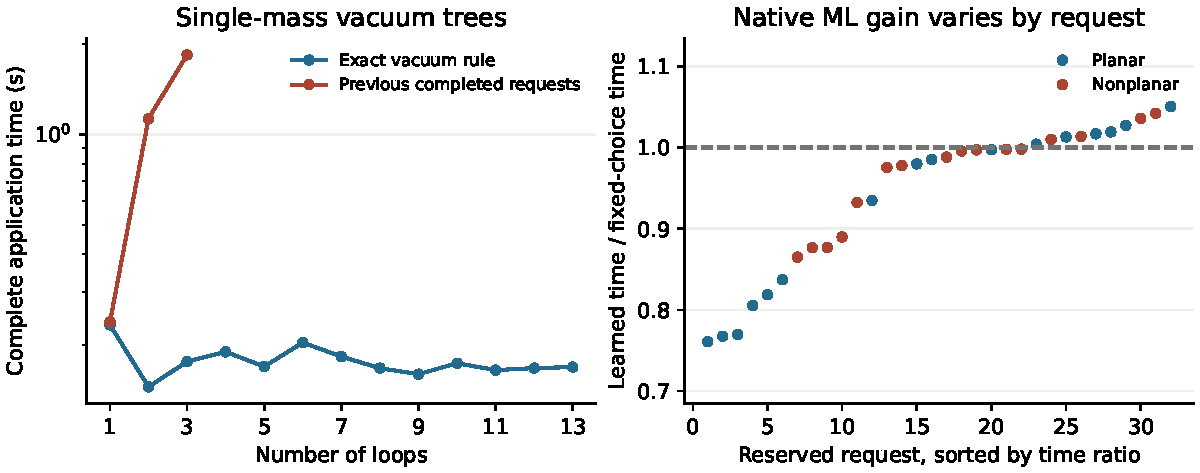
\includegraphics[width=\linewidth]{paper_figures/vacuum_learning.pdf}
\caption{The left panel shows mean request medians at each loop order for the vacuum trees; absent control points indicate that no control completed at that order. The right panel shows each matched native request relative to the fixed validation-selected seed setting. Ratios below one indicate less complete time. The equal-time line makes regressions visible.}
\label{fig:notes-vac-ml}
\end{figure}
\FloatBarrier

\section{A massive vacuum root and learned seed costs}
\label{app:notes-vac-ml}
We consider a rooted tree $T$ with $L$ loop momenta $\ell_0,\ldots,\ell_{L-1}$ and parent $\pi(j)$ for each nonroot vertex $j$. The root has one massive denominator, and every other vertex has a massless self denominator and an edge denominator:
\begin{equation}
 V_T(\mathbf a,\mathbf v,c)=
 \int\prod_{j=0}^{L-1}\frac{d^d\ell_j}{i\pi^{d/2}}
 \frac{1}{(\ell_0^2-m^2)^c}
 \prod_{j=1}^{L-1}\frac{1}{(\ell_j^2)^{a_j}
 ((\ell_j-\ell_{\pi(j)})^2)^{v_j}} .
 \label{eq:notes-vac-ml-family}
\end{equation}
Here $d$ is the dimension, $m^2>0$ is the sole mass scale, and the usual causal prescription is understood. The integer powers $c$ and $v_j$ are positive. The self powers $a_j$ are positive at leaves and can be nonpositive at internal vertices. Auxiliary numerator powers vanish. The implementation accepts one through thirteen loops and absolute powers at most sixteen. These are implementation bounds; the derivation applies to any finite tree for which the meromorphic integrals are defined.

To evaluate the integral, temporarily use denominators $-\ell^2$ for massless lines and $m^2-\ell_0^2$ for the root. Define $u_j=a_j+\sum_{h:\pi(h)=j}\sigma_h$ and $\sigma_j=u_j+v_j-d/2$. A nonroot integration then contributes the bubble factor $G(u_j,v_j)$ derived in Appendix~\ref{app:notes-prop-tree}, and transfers $\sigma_j$ to its parent. At the root, $\sigma_0=\sum_{h:\pi(h)=0}\sigma_h$. A Wick rotation gives the normalized radial integral
\begin{align}
 \frac{1}{\Gamma(d/2)}\int_0^\infty
 \frac{x^{d/2-\sigma_0-1}}{(x+m^2)^c}\,dx
 &=\frac{(m^2)^{d/2-\sigma_0-c}}{\Gamma(d/2)}
 \int_0^\infty\frac{t^{d/2-\sigma_0-1}}{(1+t)^c}\,dt \nonumber\\
 &=(m^2)^{d/2-\sigma_0-c}
 \frac{\Gamma(d/2-\sigma_0)\Gamma(\sigma_0+c-d/2)}
 {\Gamma(d/2)\Gamma(c)} .
 \label{eq:notes-vac-ml-radial}
\end{align}
The substitution is $x=m^2t$. The second equality follows from the beta integral, initially in its convergent domain and then by analytic continuation~\cite{Weinzierl2022}. Thus the dimensionless coefficient is
\begin{equation}
 C_T(\mathbf a,\mathbf v,c;d)=
 \frac{\Gamma(d/2-\sigma_0)\Gamma(\sigma_0+c-d/2)}{\Gamma(d/2)\Gamma(c)}
 \prod_{j=1}^{L-1}G(u_j,v_j).
 \label{eq:notes-vac-ml-gamma}
\end{equation}
Let $A=c+\sum_{j=1}^{L-1}(a_j+v_j)$, let $P=2L-1$ be the number of physical denominators, and let $M_T=V_T(\mathbf1,\mathbf1,1)$. The sum of all transferred powers gives the mass factor $(m^2)^{Ld/2-A}$. Restoring the original denominator signs gives $(-1)^A$; division by the unit-power master therefore gives
\begin{equation}
 V_T(\mathbf a,\mathbf v,c)=
 (-m^2)^{-(A-P)}
 \frac{C_T(\mathbf a,\mathbf v,c;d)}{C_T(\mathbf1,\mathbf1,1;d)}M_T.
 \label{eq:notes-vac-ml-ratio}
\end{equation}
The Gamma arguments have the same dimension-dependent parts for every target in a fixed tree. Their remaining differences are integers, so the recurrence $\Gamma(z+1)=z\Gamma(z)$ gives a rational function of $d$ and $m^2$. We cancel equal Gamma factors before expanding the finite products, as derived in Appendix~\ref{app:notes-gamma-cancel}. This calculation reduces the family to its unit-power master without an IBP solve. It does not evaluate a general multiscale vacuum integral.

For the native part of the method, let $x_i$ be the physical and target-power features of request $i$, and let $t_{ia}$ be its measured complete time under admissible seed choice $a$. A terminal leaf containing requests $S$ selects the action that minimizes $\sum_{i\in S}t_{ia}$. A candidate split into $S_1$ and $S_2$ reduces this training objective by
\begin{equation}
 \min_a\sum_{i\in S}t_{ia}
 -\min_a\sum_{i\in S_1}t_{ia}
 -\min_a\sum_{i\in S_2}t_{ia}.
 \label{eq:notes-vac-ml-loss}
\end{equation}
This expression follows by subtracting the two child costs from the parent cost. Unverified actions receive a cost of at least sixty seconds. Separate validation requests select tree depth, leaf size, ensemble size, and the required predicted saving. A fixed action minimizes total validation time and supplies the comparison with ML disabled. Inputs outside the training feature ranges use this fixed action. No predicted reduction coefficient enters the algebra.

The native tests use the planar and nonplanar momenta defined in Appendix~\ref{app:families}. For the planar graph, $s=2p_1\cdot p_2$ and $t=2p_1\cdot p_3$; for the nonplanar graph, $s=(p_1+p_2)^2$ and $t=(p_1-p_3)^2$. We use $s=-1009-12h$ and $t=-1021-14h$ for the planar graph, and $s=-113-18h$ and $t=-127-10h$ for the nonplanar graph. The profile is $h=6011$ for training, $6029$ for validation, $6043$ for the first reserved test, and $6079$ for the separate final application test. All values use a common squared-momentum unit. Each target has index vector $(1,1,1,1,1,1,1,-a,-b)$ with nonnegative integers $a,b$ satisfying $1\leq a+b\leq4$. The batch, rather than the individual pair $(a,b)$, defines a split member.

% END CURRENT WORKFLOW UPDATE
% BEGIN CURRENT WORKFLOW UPDATE
\section{Exact numerator reduction with learned identity choices}
\label{sec:notes-tensor-results}
The preceding scalar recurrence accepts raised denominator powers. A polynomial numerator can prevent that path from applying, even when only one loop needs reduction. We extend the exact stage to such numerators by resolving the loop momentum into directions parallel and perpendicular to the external vectors seen by the denominators. Angular averages remove the perpendicular numerator factors, after which the scalar recurrence lowers the remaining powers. Tensor reduction and general one-loop generating functions provide the established context~\cite{DennerDittmaier2006,Hu2025}; Appendix~\ref{app:notes-tensor-reduction} derives the specific angular and signed-index IBP identities used here.

There are two useful orders for these identities. We can remove the numerator before lowering raised propagator powers, or use the signed-index IBP relation to lower those powers first. In either order, the calculation ends at unit-power scalar sectors. The model selects this order and whether to lower the largest or smallest raised positive power. The implementation shares intermediate reductions within each request and reuses identical independent components within that request. Its four actions therefore change the path through exact identities. Exact arithmetic supplies every reduction coefficient. We keep the preceding native seed model for inputs that still require Kira.

We also use the derived denominator structure to simplify the exact arithmetic. Every dimension-dependent denominator is a product of factors $d+j$ with integer $j$. Keeping these factors explicit permits exact cancellation by polynomial division, as derived in Eqs.~\eqref{eq:notes-tensor-factored-field}--\eqref{eq:notes-tensor-factored-add}. The final model learns from complete timings with this arithmetic in place. A fixed-action control uses the same arithmetic, so that the measured effect of the model remains separate from the exact improvement.

\subsection{Families, checks, and comparison design}
The new one-loop families contain two, three, or four physical denominators and one or two auxiliary coordinates, with at most five coordinates in total. Numerator rank means $\sum_j\max(-a_j,0)$, and excess positive power means $\sum_j\max(a_j-1,0)$. The training requests span numerator ranks one through four and excess powers zero through three. They use distinct rational masses and off-shell scalar products, with symbolic $d$. Appendix~\ref{app:notes-tensor-reduction} specifies the construction and the wider implementation bounds. These are reductions at rational kinematic points; they do not reconstruct a general symbolic multiscale answer.

We measure all four actions on 24 training requests and 12 separate validation requests. Their mass and scalar-product profiles differ across splits, although some index patterns recur. The final test changes both the profiles and target batches. Sixteen requests use the massive training structures, four further requests use massless or mixed-mass sectors, and twelve requests use independent products of tensor bubbles at each loop order from two through thirteen. Eight new native requests test the retained seed model in planar and nonplanar massless two-loop boxes, while four vacuum-tree requests check that the preceding exact path still works. The products establish a factorized high-loop extension. Each method returns the product of component reductions, so the timed output retains the factors instead of expanding every product of master integrals. These requests do not test a coupled thirteen-loop scattering reduction.

The development checks compare 44 exact coefficients with native Kira in six requests, test 37 coefficients in independently assembled signed IBP residuals, and test changes of loop names, loop signs, and propagator order. The final arithmetic passes 240 rational-function comparisons and repeats the native pilot agreement. Every new training and validation output is compared with the first symbolic-field implementation. The reserved tensor results are checked through the alternate recurrence, while native box results use separately prepared Kira references. If a native result uses a different basis, the external check reduces that basis before comparing coefficients. These checks follow the algebra of the reduction and do not replace the derivation.

Each reserved application starts in a fresh process and runs three times, with method order rotated on the same worker. The eighteen-second limit applies to every timed method. Total time includes input reading, recognition, model loading and prediction, exact algebra or native recovery, output, and exit. The separate reference calculation and external coefficient comparison lie outside all application timers. The preceding native method uses its existing master-index registry. A failed request remains in the completion counts and receives no finite speed factor. We sum per-request median times only for requests that both methods complete and verify in all three repetitions. The resampling interval uses the request-level procedure of the request-resampling calculation defined at the end of the final-results subsection below.

\subsection{Final exact and learned results}
Validation selects 1 cost tree, depth at most 1, minimum leaf population 2, and a predicted-saving margin of 8\%. The fixed control removes the numerator first and then lowers the smallest raised positive power. The validation rule disables the new learned choice. Its validation cost, including a one-millisecond allowance per request, is 3.207 seconds, against 3.195 seconds for the fixed choice. These values determine deployment; the final test supplies the independent timing result.

The deployment rule leaves the tensor model disabled. Its final application and fixed control therefore use the same action; their timing difference measures run variation. The retained native seed model remains active on its eligible requests.

\begin{table}[!htbp]\centering\small
\caption{Final complete-time comparisons. Counts give control/final completions, and times sum medians on matched completed requests. The first tensor implementation uses a general rational-function field. The fixed control uses the final exact arithmetic with the relevant learned choice disabled. All entries are measurements of this study.}
\label{tab:notes-tensor-results}
\begin{tabularx}{\linewidth}{@{}Yrrrr@{}}\toprule
Comparison & Done & Paired & Control (s) & Final (s)\\\midrule
Tensor / preceding application & 20/20 & 20 & 53.518 & 6.343 \\
Tensor / first implementation & 20/20 & 20 & 26.703 & 6.343 \\
Independent products / preceding & 12/12 & 12 & 121.891 & 3.006 \\
Native boxes / fixed seed choice & 8/8 & 8 & 53.468 & 51.894 \\
Native boxes / preceding & 8/8 & 8 & 50.717 & 51.894 \\
All 44 requests / preceding & 44/44 & 44 & 227.011 & 62.225 \\
Vacuum regression / preceding & 4/4 & 4 & 0.885 & 0.982 \\
\bottomrule\end{tabularx}\end{table}

\begin{table}[!htbp]\centering\small
\caption{Physical scope of the final one-loop tensor comparison. Times sum matched request medians against the preceding application. Mass classes with a single request have evidence from that case alone.}
\label{tab:notes-tensor-types}
\begin{tabularx}{\linewidth}{@{}Yrrr@{}}\toprule
Integral class & Paired & Preceding (s) & Final (s)\\\midrule
Massive bubbles & 8 & 13.833 & 1.911 \\
Massive triangles & 4 & 9.020 & 1.291 \\
Massive boxes & 4 & 20.998 & 2.185 \\
Massless bubble & 1 & 1.409 & 0.212 \\
Mixed-mass bubble & 1 & 1.694 & 0.183 \\
Mixed-mass triangle & 1 & 1.981 & 0.270 \\
Mixed-mass box & 1 & 4.583 & 0.290 \\
\bottomrule\end{tabularx}\end{table}\FloatBarrier

The tensor comparison with the preceding application gives time ratio 0.119, with a central 95\% request-resampling interval of $[0.106,0.133]$. The final method is slower on 0 of 20 matched requests.

The tensor comparison with the first implementation gives time ratio 0.238, with a central 95\% request-resampling interval of $[0.214,0.262]$. The final method is slower on 0 of 20 matched requests.

The retained native seed model against fixed choices gives time ratio 0.971, with a central 95\% request-resampling interval of $[0.936,1.011]$. The final method is slower on 2 of 8 matched requests. The interval includes equal time, so this sample does not resolve a consistent gain across its requests.

The final application completes 44 of 44 requests in every repetition, with 13,272 coefficient comparisons across the timed methods. The new tensor selector makes no predictions because validation retains the fixed action. The retained seed model is evaluated on 8 of the eight native requests. The complete-time gains against the preceding application include the new exact identities and arithmetic; the native fixed control measures the extra learned choice.

Across all 44 requests, total time changes from 227.011 to 62.225 seconds, or 72.6\% less time on this collection. The final application is slower on 10 requests. The native requests take 1.023 times the preceding application's time, and the four retained vacuum requests take 1.110 times its time. These regressions remain in the overall result; the new exact tensor path supplies the large saving.

\begin{figure}[!htbp]\centering
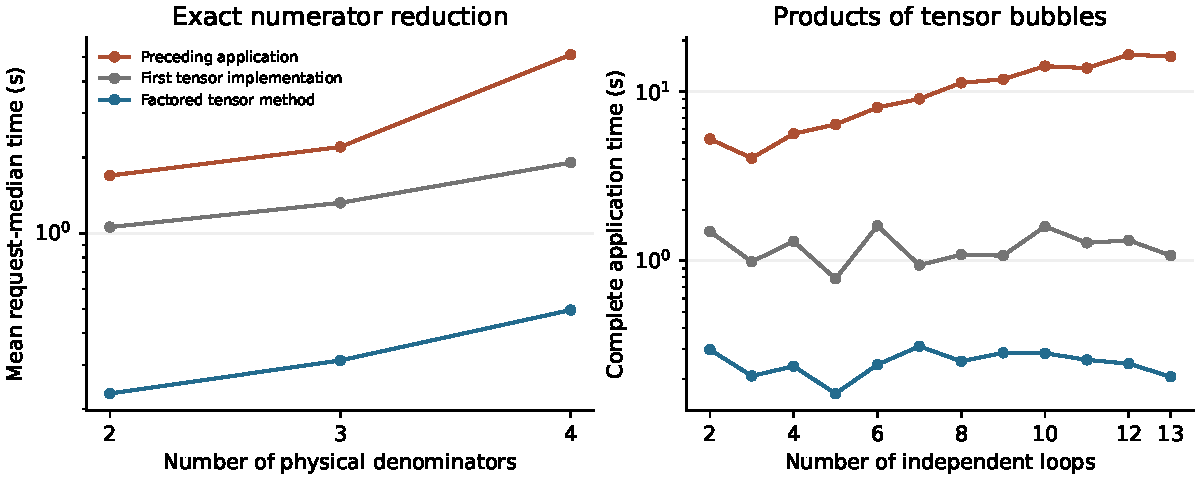
\includegraphics[width=\linewidth]{paper_figures/tensor_reduction.pdf}
\caption{Exact numerator reduction and factored dimension denominators reduce complete time on the plotted requests. The left panel averages the request medians, on common completed requests, for each physical-denominator count. The right panel shows independent tensor-bubble products through thirteen loops. Only requests completed in all repetitions appear; missing points represent incomplete controls. The logarithmic time axes show the full measured range. The fixed-control comparisons in Table~\ref{tab:notes-tensor-results} separately measure the learned contribution.}
\label{fig:notes-tensor-results}
\end{figure}
\FloatBarrier

The added exact domain covers rational one-loop numerator reductions and their independent products under the stated matrix and power conditions. The retained vacuum and massless tree identities supply further connected high-loop domains. General symbolic multiscale kinematics, singular tensor projections requiring other identities, and arbitrary coupled high-loop scattering remain outside this extension. The results establish the measured savings and their limits; they do not establish a globally shortest reduction path.

For each comparison, we resample its matched requests with replacement 2,000 times, sum the request medians in each resample, and divide the final sum by the control sum. The reported central interval uses the 2.5 and 97.5 percent quantiles of these ratios. This describes variation across the finite request collection.
\subsection{First tensor implementation and preliminary comparison}
For native, the first implementation completes 8 of 8 requests in all repetitions. Its preceding control completes 8. On 8 matched requests, the control and first tensor times are 43.859 and 43.616 seconds.
For other masses, the first implementation completes 4 of 4 requests in all repetitions. Its preceding control completes 4. On 4 matched requests, the control and first tensor times are 8.917 and 4.174 seconds.
For previous exact, the first implementation completes 4 of 4 requests in all repetitions. Its preceding control completes 4. On 4 matched requests, the control and first tensor times are 0.881 and 1.015 seconds.
For products, the first implementation completes 12 of 12 requests in all repetitions. Its preceding control completes 11. On 11 matched requests, the control and first tensor times are 111.212 and 12.690 seconds.
For tensor, the first implementation completes 16 of 16 requests in all repetitions. Its preceding control completes 16. On 16 matched requests, the control and first tensor times are 61.705 and 21.466 seconds.
The first identity-order model gives ratio 1.065 against its fixed action, with request interval $[1.039,1.097]$. Its weights remain stored, while the final arithmetic uses a separately trained policy.
The preliminary fixed-control measurement for the three-loop product contains a startup import failure during a source transfer. The outcome remains in the saved record and is excluded from completed-time comparisons. Subsequent transfers retain unchanged files and replace changed sources atomically. The final comparison uses a new collection and preserves all failures separately.

\section{Exact reduction of polynomial numerators}
\label{app:notes-tensor-reduction}
\subsection{Resolving the loop momentum}
One-loop tensor reduction expresses loop-momentum numerators through scalar integrals. Established methods include tensor decompositions and generating functions for arbitrary numerator and denominator powers~\cite{DennerDittmaier2006,Hu2025}. We derive the particular identities used in our extension here. The algebra uses rational kinematic values and keeps $d$ symbolic. It applies to a one-loop sector and to independent products of such sectors. Applying it inside a coupled graph would require coefficients that depend on the other loop momenta, which this implementation does not support.

Write $D_i=(\ell-q_i)^2-m_i^2$ and let $S=\{i:a_i>0\}$ contain the denominator positions. The $q_i$ in this appendix are fixed external shifts; the infinitesimal prescription is understood. Choose $r\in S$, set $k=\ell-q_r$, and define $R_i=q_i-q_r$. The vectors $R_i$ with $i\in S\setminus\{r\}$ span the external directions seen by the denominators. Their Gram matrix and their contractions with $k$ are
\begin{equation}
 G_{ij}=R_i\cdot R_j,\qquad
 u_i=k\cdot R_i=\frac{D_r-D_i+m_r^2-m_i^2+R_i^2}{2}.
 \label{eq:notes-tensor-u}
\end{equation}
The second equality follows by expanding $D_i=(k-R_i)^2-m_i^2$ and subtracting it from $D_r=k^2-m_r^2$. Assume that $G$ is invertible, and split $k$ into its projection onto this span and its perpendicular part:
\begin{equation}
 k_\parallel^\mu=\sum_{i,j\in S\setminus\{r\}}R_i^\mu(G^{-1})_{ij}u_j,
 \qquad k_\perp=k-k_\parallel.
 \label{eq:notes-tensor-projection}
\end{equation}
Contracting with each $R_i$ gives $k_\perp\cdot R_i=0$. Contracting the parallel part with itself gives $k_\parallel^2=u^TG^{-1}u$, so
\begin{equation}
 T(D):=k_\perp^2=D_r+m_r^2-u^TG^{-1}u.
 \label{eq:notes-tensor-radius}
\end{equation}
Empty matrices and sums give zero when $S$ has one element.

An inverse propagator $D_j$ with $a_j<0$ appears in the numerator and can be resolved into the same components. Define $v_{ji}=R_j\cdot R_i$, $R_{j,\perp}=R_j-\sum_{i,h}R_i(G^{-1})_{ih}v_{jh}$, and $z_j=k_\perp\cdot R_{j,\perp}$. Direct substitution gives
\begin{align}
 D_j&=B_j(D)-2z_j,\\
 B_j(D)&=D_r+m_r^2+R_j^2-m_j^2-2v_j^TG^{-1}u,\\
 H_{jh}&:=R_{j,\perp}\cdot R_{h,\perp}
       =R_j\cdot R_h-v_j^TG^{-1}v_h.
 \label{eq:notes-tensor-numerator}
\end{align}
Thus the remaining task is to average products of the $z_j$ over perpendicular directions. All positive-power denominators depend on $k_\perp$ only through $T(D)$, so this angular average leaves the denominator unchanged.

\subsection{Angular moments and the finite numerator expansion}
Let $\nu=d-|S|+1$ be the dimension perpendicular to the denominator span. Rotational symmetry makes odd angular moments vanish. For $2h$ perpendicular components, the invariant symmetric tensor is the sum of all pairings of metric tensors, multiplied by a coefficient $C_h T^h$. Tracing two indices gives
\begin{equation}
 C_h(\nu+2h-2)=C_{h-1},\qquad C_0=1,
 \qquad C_h=\frac{1}{\prod_{b=0}^{h-1}(\nu+2b)}.
 \label{eq:notes-tensor-trace}
\end{equation}
The trace factor contains $\nu$ from the pairing of the traced indices and $2h-2$ from their pairings with the other indices. Contracting the tensor with the external perpendicular vectors therefore gives
\begin{equation}
 \left\langle\prod_{t=1}^{2h}z_{j_t}\right\rangle
 =\frac{T(D)^h}{\prod_{b=0}^{h-1}(\nu+2b)}
 \sum_{\mathcal P}\prod_{(s,t)\in\mathcal P}H_{j_sj_t}.
 \label{eq:notes-tensor-moment}
\end{equation}
Here $\mathcal P$ runs over the distinct pairings of the $2h$ positions, including their multiplicities when an index repeats. In particular,
\begin{equation}
 \langle z_i z_j\rangle=\frac{T H_{ij}}{\nu},\qquad
 \langle z_i z_j z_k z_l\rangle
 =\frac{T^2(H_{ij}H_{kl}+H_{ik}H_{jl}+H_{il}H_{jk})}{\nu(\nu+2)}.
 \label{eq:notes-tensor-low-moments}
\end{equation}
One can first derive these relations after a Wick rotation in an integer dimension, where the angular average is well defined, and then continue the rational tensor coefficients in $d$. This uses the dimensional-regularization convention of Eq.~\eqref{eq:general-integral}~\cite{Weinzierl2022}. Poles in $d$ remain exact rational poles.

For $b_j=-a_j>0$, expand $\prod_{j:a_j<0}(B_j-2z_j)^{b_j}$ and insert Eq.~\eqref{eq:notes-tensor-moment}. The result is a finite polynomial in the positive-sector denominators:
\begin{equation}
 \left\langle\prod_{j:a_j<0}D_j^{b_j}\right\rangle
 =\sum_{\boldsymbol t}c_{\boldsymbol t}(d)\prod_{i\in S}D_i^{t_i},
 \qquad
 I_{\boldsymbol a}=\sum_{\boldsymbol t}c_{\boldsymbol t}(d)
 I_{\boldsymbol a_S-\boldsymbol t}.
 \label{eq:notes-tensor-expansion}
\end{equation}
The vector $\boldsymbol a_S$ equals $\boldsymbol a$ on $S$ and vanishes elsewhere; the $t_i$ are nonnegative and vanish outside $S$. The coefficients also depend rationally on the fixed kinematics. Each power $D_i^{t_i}$ cancels the corresponding denominator power. If a cancellation creates a new negative index, that line leaves the positive sector. Repeating the angular step therefore decreases the positive-sector size whenever a numerator remains. A sector with no denominators is scaleless and vanishes in dimensional regularization~\cite{Weinzierl2022}. The process terminates in scalar sectors with nonnegative indices.

\subsection{Lowering powers before removing the numerator}
A second exact route starts with IBP. Define $A=\sum_j a_j$ and $Y_{ij}=m_i^2+m_j^2-(q_i-q_j)^2$. Expanding the total derivative with vector $\ell-q_i$ gives
\begin{align}
 0&=d I_{\boldsymbol a}
 -\sum_j a_j\int\frac{d^d\ell}{i\pi^{d/2}}
 \frac{2(\ell-q_i)\cdot(\ell-q_j)}{D_j}\prod_hD_h^{-a_h},\\
 2(\ell-q_i)\cdot(\ell-q_j)&=D_i+D_j+Y_{ij},\\
 0&=(d-A)I_{\boldsymbol a}
 -\sum_j a_j I_{\boldsymbol a+\boldsymbol e_j-\boldsymbol e_i}
 -\sum_j a_jY_{ij}I_{\boldsymbol a+\boldsymbol e_j}.
 \label{eq:notes-tensor-ibp}
\end{align}
Here $\boldsymbol e_j$ is the unit index vector. This derivation holds for signed integer indices, so it includes numerator terms. Let $N_- =\{j:a_j<0\}$. Moving the negative-index terms to the right gives, for $i\in S$,
\begin{align}
 \sum_{j\in S}a_jY_{ij}I_{\boldsymbol a+\boldsymbol e_j}&=F_i(\boldsymbol a),\\
 F_i(\boldsymbol a)&=(d-A)I_{\boldsymbol a}
 -\sum_{j:a_j\ne0}a_j I_{\boldsymbol a+\boldsymbol e_j-\boldsymbol e_i}
 -\sum_{j\in N_-}a_jY_{ij}I_{\boldsymbol a+\boldsymbol e_j}.
 \label{eq:notes-tensor-signed-system}
\end{align}
For target $\boldsymbol b$ with $b_k>1$, choose $\boldsymbol a=\boldsymbol b-\boldsymbol e_k$. If $Y_S$ is invertible, multiply this system by its inverse to obtain
\begin{equation}
 I_{\boldsymbol b}=\frac{1}{a_k}
 \sum_{i\in S}(Y_S^{-1})_{ki}F_i(\boldsymbol a).
 \label{eq:notes-tensor-signed-recurrence}
\end{equation}
Every integral on the right has a smaller sum of positive indices than $\boldsymbol b$, and the numerator rank does not increase. When the positive powers reach one, the angular step removes the remaining numerator. With no negative indices, Eq.~\eqref{eq:notes-tensor-signed-recurrence} reduces to the scalar Cayley recurrence derived earlier. These identities give a finite reduction to unit-power scalar sectors. They produce a spanning set; special kinematics can introduce further relations between its elements.

\subsection{Scope and learned choice of identity}
The implementation admits two through five complete one-loop coordinates, rational masses and scalar products, numerator rank $\sum_j\max(-a_j,0)\leq6$, and excess positive power $\sum_j\max(a_j-1,0)\leq6$. It rejects cuts, symbolic indices, and any singular Gram or Cayley matrix required by the chosen route. Bounded recurrence work supplies a further rejection condition. Such inputs return to the preceding exact and native Kira procedure. The derivation explains the exact result on admitted inputs; it does not assert that this bounded implementation covers every one-loop family.

The four candidate actions combine numerator-first or power-first reduction with lowering the largest or smallest available raised positive power. For a request, let $x$ contain the coordinate count, target count, minimum, maximum, and mean numerator rank and excess positive power, minimum and maximum positive-sector size, largest positive index, number of distinct numerator patterns, and five coordinatewise maxima of each sign. This gives 22 features. We train regression trees whose leaves store the mean measured cost of each action, using the cost-sensitive split objective of Appendix~\ref{app:notes-fast-method} and the tree and forest constructions of Refs.~\cite{CART1984,Breiman2001Forest}. The labels include process startup, exact reduction, model use where present, output, and exit. Failed choices receive a cost of at least 60 seconds.

We compare one tree with 24 bootstrap trees, depths one through four, minimum leaf populations two, four, or eight, and fractional-saving margins zero, 0.03, 0.08, or 0.15. Each ensemble tree draws 24 requests with replacement and considers 11 of the 22 features at each split. A split must improve the empirical action cost by more than 0.002 seconds per request in its parent node. Separate validation chooses the model settings and the fixed action with the lowest total validation cost. A learned action is enabled only when its predicted cost plus one millisecond is below the fixed cost by this margin. Inputs outside the training feature ranges use the fixed action. Validation must also show at least one percent less total cost and no increase in unverified results before deployment. This rule follows by comparing predicted total costs; it changes only the order of exact identities. Section~\ref{sec:notes-tensor-results} reports whether that model improves on the fixed control in the reserved test.

\subsection{Keeping the dimension poles in factored form}
The preceding identities restrict the form of every dimension-dependent denominator. The inverse Gram and Cayley matrices have rational entries at the chosen kinematic point, and Eq.~\eqref{eq:notes-tensor-signed-recurrence} introduces only polynomial dependence on $d$. Equation~\eqref{eq:notes-tensor-moment} introduces products of linear factors $d+j$, where $j$ is an integer. By induction through the recurrence, each coefficient therefore has the form
\begin{equation}
 r(d)=\frac{P(d)}{\prod_j(d+j)^{n_j}},\qquad
 P(d)\in\Q[d],\quad n_j\in\mathbb Z_{\geq0}.
 \label{eq:notes-tensor-factored-field}
\end{equation}
The finite products contain only factors introduced by the angular moments. For addition, take $Q$ to be the least common multiple of two such denominators $Q_1$ and $Q_2$. Multiplying each summand by its missing factors gives
\begin{equation}
 \frac{P_1}{Q_1}+\frac{P_2}{Q_2}
 =\frac{P_1(Q/Q_1)+P_2(Q/Q_2)}{Q}.
 \label{eq:notes-tensor-factored-add}
\end{equation}
The exponent of $d+j$ in $Q$ is the larger of its two exponents. Multiplication adds these exponents. A factor $d+j$ cancels exactly when $P(-j)=0$, because division with remainder gives $P(d)=(d+j)\widetilde P(d)+P(-j)$. We repeat this cancellation for each retained factor. These operations preserve the exact rational function and require only rational polynomial coefficients and integer factor multiplicities. They avoid general rational-function simplification in the new path. We check the resulting coefficients against both the first symbolic-field implementation and the native pilot reductions, retrain the action model on the revised costs, and freeze a separate final test.

\subsection{Defined kinematics and target collections}
To specify the measured domain, let $P$ be the number of physical denominators and let $e$ be the number of auxiliary coordinates. We use $(P,e)=(2,1),(2,2),(3,1),(4,1)$, set $N=P+e$, and introduce $N-1$ independent external vectors $p_i$. The shifts are $q_1=0$ and $q_{i+1}=p_i$. With all squared quantities in a common fixed unit, the massive profile $h$ is defined by
\begin{align}
 m_i^2&=h+11i^2\quad(1\leq i\leq P),\\
 m_i^2&=0\quad(P<i\leq N),\\
 p_i^2&=-(10h+17i),\\
 p_i\cdot p_j&=-(h+i+2j-2)\quad(1\leq i<j<N).
 \label{eq:notes-tensor-kinematics}
\end{align}
Equation~\eqref{eq:notes-tensor-kinematics} defines the test kinematics. Their negative-definite external Gram matrices define off-shell analytic points. The mixed-mass tests retain only the odd-position physical masses, and the massless test sets them all to zero. Each target starts with unit powers on its $P$ physical denominators. We distribute $\delta$ further positive powers over these positions and $R$ negative powers over the $e$ auxiliary positions, retaining distinct targets. The requested batch size $B$ can exceed the number of distinct vectors for a small setting, in which case the batch contains the whole available set.

The training settings $(R,\delta,B)$ are $(1,0,1)$, $(1,2,2)$, $(2,1,2)$, $(2,3,3)$, $(3,1,2)$, and $(4,2,2)$. Validation uses $(1,3,2)$, $(3,2,2)$, and $(4,1,2)$. For structure position $k=0,\ldots,3$ and setting position $j$ starting at zero, training uses $h=7103+8k+j$ and validation uses $h=7301+8k+j$. The first reserved comparison uses $h=7507+8k+j$ with settings $(2,2,2)$, $(3,3,2)$, $(4,0,1)$, and $(4,3,3)$. The final comparison uses $h=7801+8k+j$ with $(1,2,2)$, $(2,3,3)$, $(3,1,2)$, and $(4,2,2)$. The final massless or mixed-mass profiles use $h=7867+P+e$, numerator rank three, and excess power one. Independent products use $L$ massive tensor bubbles with $h=7901+L$, numerator rank two, and excess power two in each component. Cross-loop auxiliary powers vanish, so the factorization follows directly from the product measure and integrand. The model receives the component requests after this exact separation.

The final native tests retain the massless planar and nonplanar box definitions of Appendix~\ref{app:families}, with profile $h=7949$ in the invariant formulas of Appendix~\ref{app:notes-vac-ml}. They use four previously unused numerator-batch sets per topology and the unchanged preceding seed policy. These tests check that the enlarged exact dispatcher preserves native ML use; they do not train that native model again.

% END CURRENT WORKFLOW UPDATE
% BEGIN CURRENT WORKFLOW UPDATE
% LIGHTLIKE EXACT AND ML UPDATE
\section{Focused exact and learned decomposition update}
The main paper now follows the physics method and its current measurements. Earlier experiments remain in these notes.

\section{Measured results}
\label{notes-light-sec:results}
The following numbers are measurements of this study. The new test holds the exact identities and the selected model fixed. Table~\ref{notes-light-tab:light-results} separates the physical groups and retains incomplete controls. A completed request must agree with its reference in every repetition.
\begin{table}[!htbp]\centering\small
\caption{Complete application times against the preceding application. Done gives preceding/new completions; times sum request medians on the matched completed subset only. A dash means no matched pair.}
\label{notes-light-tab:light-results}
\begin{tabularx}{\linewidth}{@{}Yrrrr@{}}\toprule
Requests & Done & Paired & Preceding (s) & New (s)\\\midrule
Zero-invariant tensor bubbles & 20/20 & 20 & 27.055 & 5.856 \\
Symbolic scalar masses & 3/3 & 3 & 4.564 & 3.958 \\
Independent products, 2--13 loops & 12/12 & 12 & 18.818 & 2.775 \\
Larger sectors with a zero-invariant sub-sector & 3/3 & 3 & 4.856 & 0.608 \\
Ordinary one-loop tensors & 3/3 & 3 & 0.682 & 0.708 \\
Connected vacuum checks & 3/3 & 3 & 0.586 & 1.593 \\
Native two-loop box batches & 24/24 & 24 & 196.362 & 198.313 \\
All 68 requests & 68/68 & 68 & 252.923 & 213.813 \\\bottomrule\end{tabularx}\end{table}

The new application completes 68 of 68 requests, compared with 68 for the preceding application. The comparison contains 12,978 exact coefficient checks across the timed outputs. There are 0 requests without a successful external reference. On the 68 matched requests, summed median time changes from 252.923 to 213.813 seconds, a time ratio of 0.845, or 15.5\% less time. This decrease is incremental relative to the preceding implementation on the same new requests. It is not a comparison with unmodified Kira, and percentages from earlier workloads cannot be added to it. The new application is slower on 26 matched requests. These totals describe this finite collection and include native requests where the exact extension does not apply.

\subsection{Exact identities and their integration}
The new exact domains comprise 38 requests: zero-invariant tensor bubbles, symbolic scalar masses, independent products, and embedded sub-sectors. The new method completes 38 and the preceding method completes 38. Their 38 matched requests take 55.293 and 13.197 seconds, respectively. The exact rules supply the change in this comparison; no learned action is required for these recognized inputs.

Development verifies the seven direct-formula cases against Kira, checks signed IBP residuals, and compares 60 symbolic-mass coefficients after rational substitutions. The larger-sector development check compares 36 coefficients with Kira. In the reserved test, 3 of the three embedded-sector requests complete. This checks that a formula used inside a recurrence produces the same physical reduction as native elimination.

\begin{figure}[!htbp]\centering
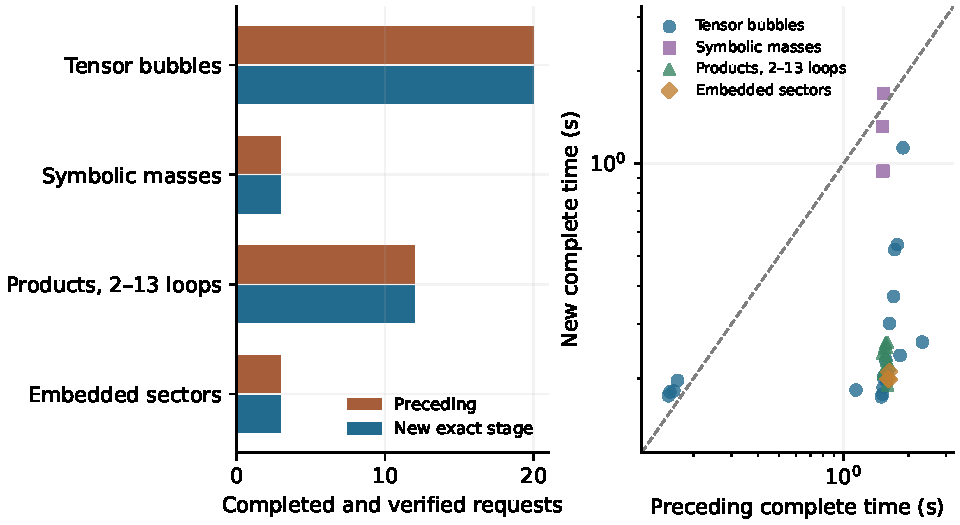
\includegraphics[width=\linewidth]{paper_figures/lightlike_exact.pdf}
\caption{Exact-extension results. The left panel compares completion counts, including failures. The right panel shows paired request times on logarithmic axes; points below the equal-time line favor the new method. Only completed, verified pairs appear in the time panel.}
\label{notes-light-fig:light-exact}
\end{figure}
\subsection{The added native ML choice}
Validation selects 1 cost tree with maximum depth 2, minimum leaf population 2, a saving margin of 0\%, and a failure score threshold of 0.15. It enables the new model. The selected validation cost, including the prediction allowance and any failure penalties, is 105.848 seconds; the fixed choice gives 107.356 seconds. The selected fixed region is tight. These values determine deployment before the reserved test.

In the 24 reserved native batches, the integrated method uses the new model on 24 requests in the final repetition. Against the fixed-choice application, it completes 24 requests while the control completes 24. The 24 matched batches take 200.983 seconds with the fixed choice and 198.313 seconds with the integrated choice. The ratio is 0.987, with a central 95\% request-resampling interval of $[0.970,1.002]$. It is slower on 11 matched batches. The interval includes equal time, so this sample does not resolve a consistent additional saving. The exact formulas and native reduction interface are shared by these two controls. The learned failure check redirects predicted risky actions and inputs outside the new feature range to the verified fixed choice.

Across the 72 native applications per method, the integrated method has 0 unverified applications, the fixed control has 0, and the preceding application has 0. In the final repetition, the recorded rejection counts are 1 for predicted failure risk and 10 for inputs outside the training feature range. These checks occur before the selected native reduction. The measured failure counts, rather than a zero predicted risk, determine whether failures were avoided in this test.

The learned policy changes the fixed action on 1 of the 24 native requests in the final repetition. Its median measured loading and decision time is 3.877 milliseconds. The saved final-repetition outputs give failed inner-attempt counts of 1 for the integrated method, 2 for the fixed control, and 0 for the preceding method. Interrupted outputs can lack inner-attempt records and remain in the separate application-failure counts. Inner attempts from the first two repetitions are not retained, so these inner-attempt counts refer only to the last repetition.

Against the preceding native application, the 24 matched batches change from 196.362 to 198.313 seconds. This comparison measures the change in the deployed policy, while the fixed control measures learned selection against one preselected region. Neither comparison measures a new elimination-row policy.

\begin{figure}[!htbp]\centering
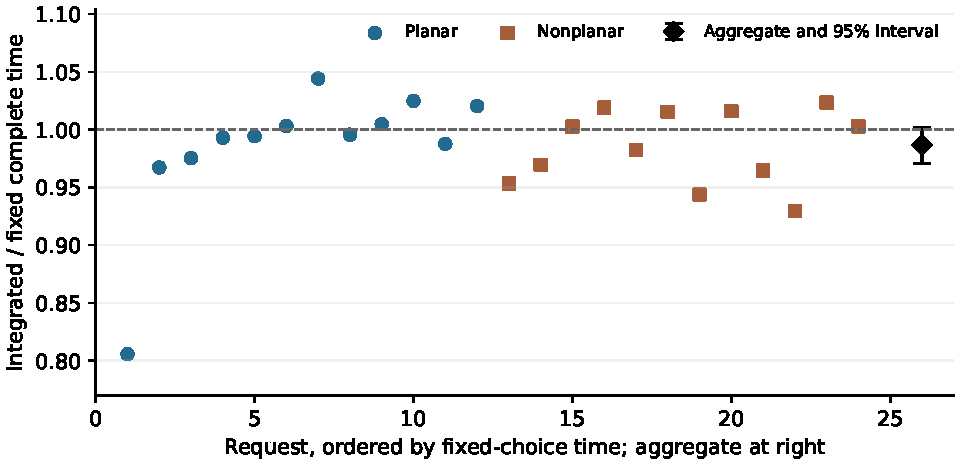
\includegraphics[width=.96\linewidth]{paper_figures/lightlike_native.pdf}
\caption{The native learned-choice comparison holds exact formulas and the native reduction interface fixed. Each point divides a request's integrated median time by its fixed-choice median. The horizontal line marks equal time. The aggregate ratio and its request-resampling interval appear separately; individual points show the observed variation across batches.}
\label{notes-light-fig:light-native}
\end{figure}
\subsection{The other learned interventions}
Table~\ref{notes-light-tab:retained-results} retains the main earlier controls needed to interpret the method. They use different workloads and cannot be multiplied into a cumulative speed factor. The equation-filter result supports that intervention on its tested domain, while the row results motivate its omission. The current combined experiment keeps equation filtering off and does not claim a joint seed-plus-equation gain.
\begin{table}[!htbp]\centering\small
\caption{Earlier measurements from this study, retained as separate evidence. A ratio below one means less time. Their full input definitions and measurements remain in the notes.}
\label{notes-light-tab:retained-results}
\begin{tabularx}{\linewidth}{@{}YYr@{}}\toprule
Intervention & Control and workload & Time ratio\\\midrule
Earlier native seed model & Fixed region, 32 box batches: 156.383 to 150.663 s & 0.963\\
Equation selection & Native filter, 24 new-index batches: 72.295 to 67.478 s & 0.933\\
Original learned row model & Native row choices, 84 trials & 1.305\\
Compiled row-cost policy & Native row choices; geometric mean & 0.982\\\bottomrule
\end{tabularx}
\end{table}
The earlier seed comparison has interval $[0.937,0.984]$, and the equation comparison has interval $[0.928,0.940]$. The compiled row policy has interval $[0.959,1.003]$, which includes equal time. These intervals use the resampling procedure recorded for each original study. The native row algorithm remains in the retained workflow.

\subsection{Scope of the result}
The new exact identities cover their stated masses, powers, and kinematics, and the reserved comparison tests concrete instances of those identities. The independent products reach thirteen loops by factorization, while the connected vacuum checks use a one-scale tree. General coupled multiscale scattering at every loop order remains outside this evidence. The native build also has a finite integral-coordinate limit, documented in the notes; a loop count alone does not determine whether an arbitrary family can be reduced.

The learned test uses two graph types already represented during training, with new whole target batches and kinematic points. It does not establish transfer to every topology. The application keeps exact algebra and bounded recovery for supported native inputs, but neither a finite training search nor the present timings prove globally minimal reduction time. The practical result is a tested extension of the exact domain together with a separately measured policy for the remaining native work.
\FloatBarrier

\section{Measured-cost learning}
\label{notes-light-app:shared}
Let $C_{ia}$ be the measured complete time of training request $i$ under action $a$. Unverified actions receive $C_{ia}\geq60$ seconds. This is a training penalty, and test failures are reported as failures. A leaf containing requests $S$ assigns action cost
\begin{equation}
 \widehat C_a(S)=\frac{1}{|S|}\sum_{i\in S}C_{ia},\qquad
 a_S=\arg\min_a\sum_{i\in S}C_{ia}.
 \label{notes-light-eq:cost-leaf}
\end{equation}
The second formula follows because the first denominator does not depend on the action. A proposed split $S=S_1\cup S_2$ improves the empirical chosen cost by
\begin{equation}
 \Delta(S_1,S_2)=\min_a\sum_{i\in S}C_{ia}
 -\min_a\sum_{i\in S_1}C_{ia}
 -\min_a\sum_{i\in S_2}C_{ia}.
 \label{notes-light-eq:cost-split}
\end{equation}
This is the parent cost minus the sum of child costs. We require $\Delta>0.002|S|$ seconds before splitting. This cost-sensitive objective uses the recursive tree and bootstrap-ensemble constructions of Refs.~\cite{CART1984,Breiman2001Forest}.

For each target, let $u$ and $v$ be its two nonnegative auxiliary numerator powers and let $R=u+v$. The 21 inputs are batch size; minimum, maximum, and mean $R$; number of distinct $R$ values; minimum, maximum, and mean of each of $u,v$; counts with $u=0$ and $v=0$; sums of $uv$ and $(u-v)^2$; number of physical propagators containing both loops; largest number of physical propagators incident on a loop; and counts with $R=1,2,3,4$. All are available before reduction.

We compare 1, 12, or 32 trees, maximum depths 1 through 5, minimum leaf populations 2, 4, or 8, and required fractional savings $\eta=0,0.03,0.08,0.15$. An ensemble averages leaf cost vectors. A single tree uses the complete training set; each ensemble tree samples training requests with replacement. The fixed action $b$ minimizes total validation cost among actions that completed every training and validation request. If $a_*$ has the least predicted cost, we choose it only when
\begin{equation}
 \widehat C_{a_*}+0.002 < (1-\eta)\widehat C_b.
 \label{notes-light-eq:cost-margin}
\end{equation}
The allowance is two milliseconds per prediction during selection. Equation~\eqref{notes-light-eq:cost-margin} is the defined minimum predicted saving, obtained by adding prediction overhead to the selected cost. Validation compares candidates by unverified count, complete cost, tree count, and depth, in that order. Deployment additionally requires at least one percent less validation cost and a change from the fixed action. We also fit a failure classifier for each action from its verified/unverified training labels. Each classifier has twelve trees of depth at most three and at least two requests per child. One tree uses all requests, and eleven use bootstrap samples. A leaf returns its failed fraction $p_f$. Binary Gini impurity for $n$ requests with $k$ failures is
\begin{equation}
 n\left[1-(k/n)^2-(1-k/n)^2\right]=\frac{2k(n-k)}{n}.
 \label{notes-light-eq:failure-gini}
\end{equation}
The equality follows by expansion. Splits maximize the decrease in this quantity, following the classification-tree construction of Ref.~\cite{CART1984}. Averaging the leaf fractions gives an empirical risk score for each action, without a claim of calibrated failure probability. Validation selects a threshold from $0,0.05,0.15,0.30$ jointly with the cost policy. If the proposed score exceeds that threshold, or any feature lies outside its training range, the policy selects the fully verified fixed region. Validation requires no unverified selected actions before enabling the model. This guard uses observed evidence; a zero score is not a proof that an unseen reduction will complete. The application timer includes both predictions and any subsequent recovery.

\section{Physical test inputs}
\label{notes-light-app:families-new}
All profiles below define squared quantities in a common fixed unit. The zero-invariant families use shifts $(0,p,q,r)$ and masses $(x,y,0,0)$, with
\begin{align}
 &p^2=0,\quad p\cdot q=-h-1,\quad p\cdot r=-h-2,\nonumber\\
 &q^2=-2h-7,\quad q\cdot r=-h-3,\quad r^2=-3h-13.
 \label{notes-light-eq:light-input}
\end{align}
The unequal case has $(x,y)=(h+3,h+11)$, the equal case $(h+3,h+3)$, the mixed case $(h+3,0)$, and the massless case $(0,0)$. Targets have the form $(1+\delta_1,1+\delta_2,-b_1,-b_2)$ with $\delta_1+\delta_2=\delta$ and $b_1+b_2=R$. For class position $j=0,1,2,3$, we use $R=0,\ldots,4$, $\delta=\min(R,3)$, and $h=211+17j+R$. Each batch contains at most three distinct assignments. These definitions give the 20 tensor requests.

The three symbolic requests retain the same zero-invariant geometry with $h=301,302,303$ and squared masses $(x,y)$, $(x,x)$, and $(x,0)$ as symbols. Their positive-power pairs are $(1,1),(2,1),(1,2),(2,2)$, with zero numerator powers. Independent products contain $L$ identical components at $h=351+L$, $R=2$, and $\delta=1$, with unequal masses for odd $L$ and equal masses for even $L$. Each target is a product of the same component assignment, and $L=2,\ldots,13$. No factor connects different loop momenta.

The embedded-sector requests promote the $q$ line to a physical denominator with squared mass $421+j$ and use $h=391+j$ in the three nonzero-mass classes, $j=0,1,2$. Their targets are $(2,1,1,-1)$, $(1,2,1,-1)$, and $(2,1,0,-1)$. The first two require a three-line reduction, and the last explicitly tests its zero-invariant sub-sector.

The ordinary tensor checks have $P=2,3,4$ physical lines, one auxiliary coordinate, shifts $q_1=0$, $q_{i+1}=p_i$, and profile $h=433+P$. Their masses and scalar products are
\begin{equation}
 m_i^2=h+11i^2\ (i\leq P),\quad m_{P+1}^2=0,\quad
 p_i^2=-(10h+17i),\quad p_i\cdot p_j=-(h+i+2j-2)\ (i<j).
 \label{notes-light-eq:ordinary-input}
\end{equation}
Targets have numerator rank two and one excess positive power. The unchanged connected-vacuum checks use chains at $L=1,7,13$, the family of Appendix~\ref{app:notes-vac-ml}, and four target assignments per request. The input records retain the exact integer assignments for every batch in this finite comparison.

For the native planar box, let $p_1,p_2,p_3$ be massless, $2p_1\cdot p_2=s$, $2p_1\cdot p_3=t$, and $2p_2\cdot p_3=-s-t$. The seven physical line momenta are
\begin{equation}
 (\ell_1,\ell_1-p_1,\ell_1-p_1-p_2,\ell_2,
 \ell_2-p_1-p_2,\ell_2-p_1-p_2-p_3,\ell_1-\ell_2),
 \label{notes-light-eq:planar-input}
\end{equation}
and the auxiliary momenta are $(\ell_1-p_3,\ell_2-p_1)$. The nonplanar routing follows Ref.~\cite{KiraOriginal}:
\begin{align}
 (Q_1,\ldots,Q_9)=(&\ell_1,\ell_2,p_1-\ell_1,p_2-\ell_2,
 p_1+p_2-p_3-\ell_1,\nonumber\\
 &p_1-\ell_1+\ell_2,p_1-p_3-\ell_1+\ell_2,
 \ell_1-p_3,\ell_2-p_1-p_2).
 \label{notes-light-eq:nonplanar-input}
\end{align}
The first seven entries are physical and all masses vanish. Its convention gives $p_i^2=(p_1+p_2-p_3)^2=0$, $s=(p_1+p_2)^2$, and $t=(p_1-p_3)^2$. Expanding the squares gives $2p_1\cdot p_3=-t$ and $2p_2\cdot p_3=s+t$. The planar profiles use $(s,t)=(-1009-12h,-1021-14h)$ and the nonplanar profiles use $(-113-18h,-127-10h)$.

Every native target is $(1,1,1,1,1,1,1,-u,-v)$ with $u,v\geq0$ and $1\leq u+v\leq4$. Distinct batches contain one to six targets. Training uses 16 batches per graph at $h=19079$ and one additional batch per graph at $h=19083$ with numerator powers $(u,v)=(0,2),(0,3),(0,4)$, validation uses eight per graph at $h=19121$, and testing uses 12 per graph at $h=19139$. We exclude whole batches used by the preceding native and tensor studies. The same graph types occur in all three new splits, so the test measures new batches and kinematic points within these structures rather than transfer to an unseen topology.

\section{Time ratios and uncertainty}
\label{notes-light-app:statistics}
Let $T_{imr}$ be complete elapsed time for request $i$, method $m$, and repetition $r$. For the set $\mathcal C$ completed by both methods in all repetitions, define
\begin{equation}
 S_m=\sum_{i\in\mathcal C}\operatorname{median}_{r=1,2,3}T_{imr},\qquad
 R=\frac{S_{\rm new}}{S_{\rm control}},\qquad
 \text{fractional saving}=1-R.
 \label{notes-light-eq:time-ratio}
\end{equation}
These definitions compare identical completed requests. Dividing both times by the control time gives $R$, and subtracting gives the fractional saving. Completion counts remain separate because an unfinished reduction has no verified finite speedup. To estimate variation across requests, we draw $|\mathcal C|$ paired request indices with replacement and recompute $R$. We report the central 95\% of 2,000 such ratios, using the bootstrap construction of Ref.~\cite{Efron1979}. This interval describes the sampled request collection and does not establish performance for every integral family.

\section{Exact reduction at a zero two-point invariant}
\label{notes-light-app:lightlike}
A singular Gram matrix prevents the projection used by the generic tensor recurrence. For a two-point sector with $p^2=0$, Feynman parameters give a direct reduction to tadpoles. Degenerate one-loop kinematics require such separate identities~\cite{DennerDittmaier2006}. We derive the identity used in this study below. It applies to a polynomial numerator and two positive denominator powers; it does not assume that the two masses differ.

\subsection{Scalar integrals and mass derivatives}
Let $x$ and $y$ denote squared masses, and define
\begin{equation}
 T(x)=\int\frac{d^d\ell}{i\pi^{d/2}}\frac{1}{\ell^2-x+i0},\qquad
 B_{ab}(x,y)=\left.\int\frac{d^d\ell}{i\pi^{d/2}}
 \frac{1}{(\ell^2-x+i0)^a[(\ell-p)^2-y+i0]^b}\right|_{p^2=0}.
 \label{notes-light-eq:light-def}
\end{equation}
Here $a,b$ are positive integers. Dimensional regularization sets $T(0)=0$. With the normalization in Eq.~\eqref{eq:general-integral}, Wick rotation and the radial beta integral give~\cite{Weinzierl2022}
\begin{equation}
 T(x)=-\Gamma(1-d/2)(x-i0)^{d/2-1}.
 \label{notes-light-eq:light-tad}
\end{equation}
For $a=b=1$, combine the denominators with a parameter $z$ and shift $\ell=k+(1-z)p$. The combined squared mass is $M^2(z)=zx+(1-z)y$, because $p^2=0$. Integrating over $k$ and then $z$ gives
\begin{align}
 B_{11}(x,y)
 &=\Gamma(2-d/2)\int_0^1 [zx+(1-z)y-i0]^{d/2-2}\,dz\nonumber\\
 &=\frac{T(x)-T(y)}{x-y},\qquad x\ne y.
 \label{notes-light-eq:light-difference}
\end{align}
The second equality follows from the elementary antiderivative of a power and $\Gamma(2-d/2)=(1-d/2)\Gamma(1-d/2)$. Differentiating a propagator with respect to its squared mass raises its power. Therefore
\begin{equation}
 B_{ab}(x,y)=\frac{\partial_x^{a-1}\partial_y^{b-1}B_{11}(x,y)}{(a-1)!(b-1)!}.
 \label{notes-light-eq:light-derivative}
\end{equation}
This operation preserves a rational combination of $T(x)$ and $T(y)$ because $\partial_xT(x)=(d/2-1)T(x)/x$. We take the derivatives before imposing relations between the masses. If $x=y\ne0$, the combined mass is independent of $z$, and the beta integral instead gives
\begin{equation}
 B_{ab}(x,x)=T_{a+b}(x),\qquad
 T_n(x)=\frac{\prod_{j=1}^{n-1}(d/2-j)}{(n-1)!\,x^{n-1}}T(x).
 \label{notes-light-eq:light-equal}
\end{equation}
The formula for $T_n$ also follows by differentiating Eq.~\eqref{notes-light-eq:light-tad}. These identities support independent symbolic squared masses as well as rational values. A relation involving distinct symbolic masses is a generic rational identity; equal masses use Eq.~\eqref{notes-light-eq:light-equal} directly.

\subsection{Polynomial numerators}
Let $P(\ell)$ be a polynomial numerator. Combining the two denominators gives
\begin{equation}
 B_{ab}[P]=\frac{\Gamma(A)}{\Gamma(a)\Gamma(b)}\int_0^1 dz\,
 z^{a-1}(1-z)^{b-1}\int\frac{d^dk}{i\pi^{d/2}}
 \frac{P(k+(1-z)p)}{[k^2-M^2(z)+i0]^A},\quad A=a+b.
 \label{notes-light-eq:light-parameter}
\end{equation}
For an auxiliary inverse propagator $(\ell-q_j)^2-m_j^2$, put $w_j=(1-z)p-q_j$. Its numerator factor becomes $k^2+2k\cdot w_j+w_j^2-m_j^2$. Both $w_i\cdot w_j$ and $w_j^2-m_j^2$ are polynomials of degree at most one in $z$ when $p^2=0$.

Rotational covariance gives zero for odd moments of $k$. Tracing two indices of an even moment determines its normalization recursively: if its pairing coefficient is $C_h$, then $C_h(d+2h-2)=C_{h-1}$ and $C_0=1$. Consequently,
\begin{equation}
 \left\langle\prod_{j=1}^{2h}(k\cdot w_j)\right\rangle
 =\frac{(k^2)^h}{\prod_{r=0}^{h-1}(d+2r)}
 \sum_{\mathcal P}\prod_{(i,j)\in\mathcal P}w_i\cdot w_j,
 \label{notes-light-eq:light-angular}
\end{equation}
where $\mathcal P$ runs over pairings of the $2h$ positions. The trace recurrence follows because one pairing contributes $d$ and the remaining contractions contribute $2h-2$. This also derives the full-dimensional form of the angular identity used in Appendix~\ref{app:notes-tensor-reduction}.

After the finite numerator expansion and angular average, define $c_{ht}(d)$ by
\begin{equation}
 \langle P(k+(1-z)p)\rangle=\sum_{h,t}c_{ht}(d)(k^2)^h z^t.
 \label{notes-light-eq:light-polynomial}
\end{equation}
These coefficients also depend on the fixed external scalar products and numerator masses. They contain no loop momentum. To integrate each term, Wick rotate the radial integral, set $u=k_E^2/M^2$, and use
$\int_0^\infty u^{\alpha-1}(1+u)^{-A}du=\Gamma(\alpha)\Gamma(A-\alpha)/\Gamma(A)$ with $\alpha=d/2+h$. This gives
\begin{equation}
 J_{Ah}(M^2)=\int\frac{d^dk}{i\pi^{d/2}}\frac{(k^2)^h}{(k^2-M^2+i0)^A}
 =(-1)^{A-h}\frac{\Gamma(d/2+h)\Gamma(A-h-d/2)}{\Gamma(d/2)\Gamma(A)}
 (M^2-i0)^{d/2+h-A}.
 \label{notes-light-eq:light-radial}
\end{equation}
The initial convergence region defines the integrals; analytic continuation gives the dimensional-regularization identity outside that region~\cite{Weinzierl2022}.

For $x\ne y$, set $\Delta=x-y$, $\rho=h-A+1$, and $\lambda=d/2-1$. Expand $(1-z)^{b-1}$ and then substitute $u=y+\Delta z$. For an integer $k\ge0$,
\begin{equation}
 \int_0^1 z^k(y+\Delta z)^{\lambda+\rho}\,dz
 =\frac{1}{\Delta^{k+1}}\sum_{j=0}^k\binom{k}{j}(-y)^{k-j}
 \frac{x^{\lambda+\rho+j+1}-y^{\lambda+\rho+j+1}}{\lambda+\rho+j+1}.
 \label{notes-light-eq:light-endpoints}
\end{equation}
This follows by expanding $(u-y)^k$ and integrating each power of $u$. Dividing by the tadpole normalization in Eq.~\eqref{notes-light-eq:light-tad}, define
\begin{equation}
 R_h=\frac{(-1)^{A-h+1}(d/2)_h(1-d/2)_{A-h-1}}{(a-1)!(b-1)!},
 \qquad (z)_n=\frac{\Gamma(z+n)}{\Gamma(z)}.
 \label{notes-light-eq:light-factor}
\end{equation}
For a negative integer $n$, the last ratio means the inverse finite product $1/\prod_{r=1}^{-n}(z-r)$. Equations~\eqref{notes-light-eq:light-parameter}--\eqref{notes-light-eq:light-endpoints} now give the explicit rational reduction
\begin{align}
 B_{ab}[P]&=\sum_{h,t}c_{ht}(d)R_h\sum_{v=0}^{b-1}(-1)^v\binom{b-1}{v}
 \nonumber\\ &\quad\times\sum_{j=0}^{k}\binom{k}{j}\frac{(-y)^{k-j}}{\Delta^{k+1}}
 \frac{x^{\rho+j+1}T(x)-y^{\rho+j+1}T(y)}{\lambda+\rho+j+1},\nonumber\\[-2pt]
 &\quad k=a-1+t+v.
 \label{notes-light-eq:light-final}
\end{align}
If one mass is zero, its endpoint vanishes in a convergence region and hence by analytic continuation; the implementation omits that scaleless endpoint before evaluating powers. If both masses vanish, the sector is scaleless. For equal nonzero masses, use the beta integral directly:
\begin{equation}
 B_{ab}[P]=\sum_{h,t}c_{ht}(d)R_h\,
 \frac{\Gamma(a+t)\Gamma(b)}{\Gamma(A+t)}x^{h-A+1}T(x).
 \label{notes-light-eq:light-equal-tensor}
\end{equation}
Thus the equal-mass rule has no division by $x-y$. A sector with one positive denominator uses Eq.~\eqref{notes-light-eq:light-radial} and the same angular expansion without a Feynman parameter.

At rational kinematics, the coefficients have polynomial numerators in $d$ and products of integer-shift linear factors $d+j$ in their denominators. The finite products in Eqs.~\eqref{notes-light-eq:light-angular} and \eqref{notes-light-eq:light-factor}, and the linear denominator in Eq.~\eqref{notes-light-eq:light-endpoints}, prove this statement. We therefore use the exact factored arithmetic of Appendix~\ref{app:notes-tensor-reduction}. The implemented tensor domain has at most five coordinates, numerator rank at most four, and at most four extra positive powers. Symbolic masses currently use the scalar derivative identity. Inputs outside these conditions continue through the existing exact rules and Kira.

% LIGHTLIKE EXACT AND ML UPDATE END
% END CURRENT WORKFLOW UPDATE
% BEGIN CURRENT WORKFLOW UPDATE
% DIRECT ANALYTIC UPDATE
\section{Direct analytic evaluation and complete native regions}
The following update retains the new method, comparisons, and derivations.
\section{Measured results}
\label{notes-direct-sec:results}
The following values are measurements from the frozen comparison in this study. Table~\ref{notes-direct-tab:direct-times} separates the physical domains and includes completion counts. Summed median times refer only to the matched completed requests.
\begin{table}[!htbp]\centering\small
\caption{Complete times against the preceding application. Done gives preceding/integrated completions. Each domain uses the same requests for both methods.}
\label{notes-direct-tab:direct-times}
\begin{tabularx}{\linewidth}{@{}Yrrrr@{}}\toprule
Domain & Done & Paired & Preceding (s) & Integrated (s)\\\midrule
Two-mass products, 1--13 loops & 13/13 & 13 & 2.271 & 1.935 \\
Connected vacuum trees, 1--13 loops & 34/34 & 34 & 7.900 & 5.719 \\
Zero-invariant tensor bubbles & 3/3 & 3 & 0.577 & 0.569 \\
Ordinary one-loop tensors & 3/3 & 3 & 0.688 & 0.698 \\
Native two-loop boxes & 16/16 & 16 & 100.514 & 100.353 \\
All 69 requests & 69/69 & 69 & 111.950 & 109.273 \\\bottomrule\end{tabularx}\end{table}

On the 69 matched requests, the integrated-to-preceding time ratio is 0.976, with a central 95\% request-resampling interval of $[0.952,0.990]$. The point estimate corresponds to 2.4\% less time. The integrated application is slower on 15 matched requests. This is an incremental comparison with the preceding application on these inputs, rather than a new comparison with unmodified Kira. Earlier percentages use other workloads and cannot be added to this change.

\subsection{Direct formulas and their high-loop scope}
The two-mass product grid changes from 2.271 to 1.935 seconds on 13 matched requests. Direct partial fractions avoid generic one-loop reduction and its preparation for these inputs. The connected vacuum grid changes from 7.900 to 5.719 seconds on 34 matched requests. The connected identity is preserved, while its early dispatch avoids generic symbolic preparation when the simpler tree formula already applies. Both grids contain every loop order from one through thirteen.

The separate analytic coverage grid completes 26 of 26 requests and takes 5.983 seconds in summed median time. Its thirteen repeated-mass requests use an independent symbolic partial-fraction reference, while thirteen coupled massless vacuum requests use the scaleless-integral identity. We report this as exact-domain coverage without assigning a speedup over an unsupported native input. The implementation returns Gamma-function values for the resulting tadpoles and the connected one-mass tree masters, so these domains have an analytic value as well as a decomposition.

The tests contain 14,922 coefficient comparisons across timed outputs. Development additionally checks 48 rational-function identities, 138 product coefficients, 4 native tadpole coefficients, 6 native scaleless target relations, and two convergent radial integrals. These checks test algebra and normalization separately.

\begin{figure}[!htbp]\centering
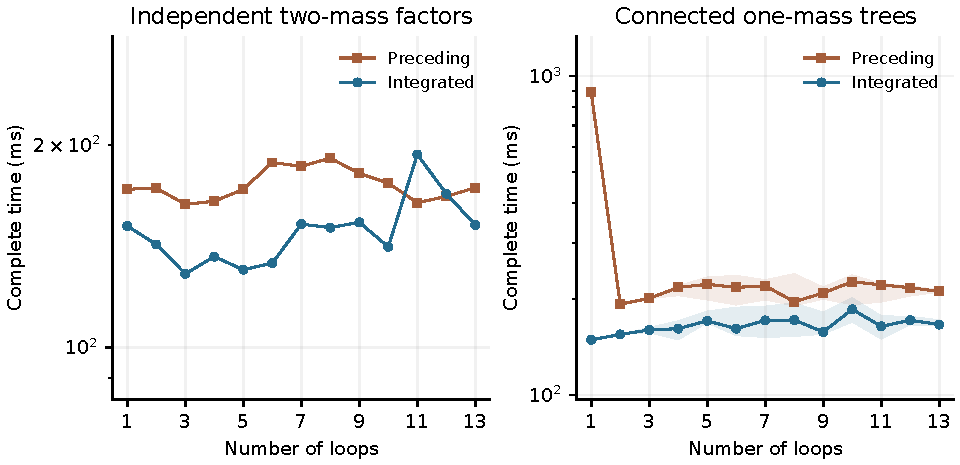
\includegraphics[width=\linewidth]{paper_figures/direct_vacuum.pdf}
\caption{Direct formulas reduce aggregate time in both measured vacuum grids. The panels show complete elapsed time at every tested loop order, with independent factors on the left. In the connected-tree panel, each line gives the median across the tested shapes at that loop order and the shaded band gives their full range. Logarithmic time axes retain the short exact calculations and the slower preparation costs. These domains require the structures stated in the derivations.}
\label{notes-direct-fig:direct-vacuum}
\end{figure}
\subsection{Native seed choices and the ML contribution}
The preliminary ordering experiment verifies all 32 development reductions. Ordering 1 has the lowest sum of development times, so the final native actions retain it. The subsequent model chooses the seed procedure. Validation selects 1 cost tree with maximum depth 1 and a minimum leaf population of 2. Its fixed control is the tight sparse region. The selected validation cost is 86.114 seconds, including the prediction allowance and failure penalties; the fixed control gives 86.090 seconds. Validation rejects the replacement because the deployment condition is not met. The final application retains the preceding validated native seed model.

On the 16 matched reserved native batches, the fixed application takes 100.166 seconds and the integrated application takes 100.353 seconds. Their ratio is 1.002, with interval $[0.994,1.012]$. This interval includes equal time and does not resolve a consistent additional learned saving. The integrated method is slower on 7 matched batches. The retained native policy changes the fixed action on 0 of the sixteen requests in the final repetition. Thus the retained model selects the fixed action throughout this final sample; the measured difference includes prediction overhead and run-to-run variation, and supplies no additional learned speedup. Median measured model loading and decision time is 2.661 milliseconds. Exact formulas, the native interface, and recovery checks are shared by the learned and fixed controls.

Across 48 native applications per method, unverified output counts are 0 for the integrated application, 0 for the fixed control, and 0 for the preceding application. Recorded failed inner attempts total 0, 0, and 0, respectively. A terminated application can lack an inner-attempt record and remains in the separate application-failure count. Complete-region selection can avoid a sparse failure, but these measurements do not guarantee success for unseen inputs.

\begin{figure}[!htbp]\centering
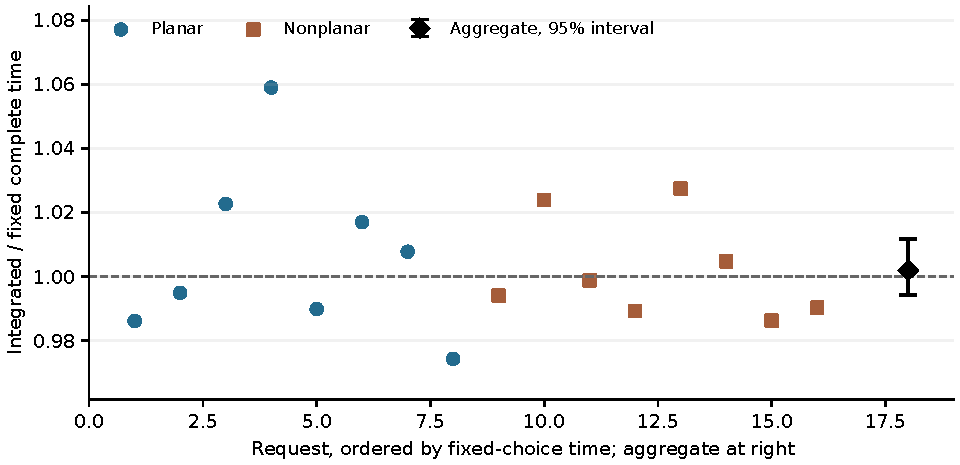
\includegraphics[width=.96\linewidth]{paper_figures/direct_native.pdf}
\caption{The retained model chooses the fixed action on every final batch, so this sample demonstrates no additional ML saving. Both controls use the same exact methods and native implementation. Points below one indicate a lower measured integrated time. Individual batches show variation, while the aggregate point reports the ratio of summed median times and its request-resampling interval.}
\label{notes-direct-fig:direct-native}
\end{figure}
\subsection{The other learned interventions}
Table~\ref{notes-direct-tab:retained-results} retains the main earlier controls needed to interpret the method. They use different workloads and cannot be multiplied into a cumulative speed factor. The equation-filter result supports that intervention on its tested domain, while the row results motivate its omission. The current combined experiment keeps equation filtering off and does not claim a joint seed-plus-equation gain.
\begin{table}[!htbp]\centering\small
\caption{Earlier measurements from this study, retained as separate evidence. A ratio below one means less time. Their full input definitions and measurements remain in the notes.}
\label{notes-direct-tab:retained-results}
\begin{tabularx}{\linewidth}{@{}YYr@{}}\toprule
Intervention & Control and workload & Time ratio\\\midrule
Earlier native seed model & Fixed region, 32 box batches: 156.383 to 150.663 s & 0.963\\
Equation selection & Native filter, 24 new-index batches: 72.295 to 67.478 s & 0.933\\
Original learned row model & Native row choices, 84 trials & 1.305\\
Compiled row-cost policy & Native row choices; geometric mean & 0.982\\\bottomrule
\end{tabularx}
\end{table}
The earlier seed comparison has interval $[0.937,0.984]$, and the equation comparison has interval $[0.928,0.940]$. The compiled row policy has interval $[0.959,1.003]$, which includes equal time. These intervals use the resampling procedure recorded for each original study. The native row algorithm remains in the retained workflow.

\subsection{Scope of the result}
The direct formulas prove reductions and analytic values within their stated domains. The test covers every loop order through thirteen for independent vacuum products and connected one-mass trees. The native test covers new target batches and kinematic points within two known two-loop scattering graphs. General coupled multiscale scattering at every loop order remains outside this evidence. Loop count alone does not classify the difficulty or determine whether a particular exact rule applies.

The controls separate changes in the integrated application from the additional effect of learned selection. A finite search over models and native settings cannot establish globally minimum time for every integral. The retained measurements include slower requests, unsuccessful attempts, and incomplete applications so that these limits remain part of the result.
\FloatBarrier

\section{IBP identities, row operations, and exactness}
\label{notes-direct-app:derivation}
The starting total-derivative identity follows from integration by parts in a region where the integral converges, followed by dimensional analytic continuation~\cite{ChetyrkinTkachov,Weinzierl2022}. Write $P_{\boldsymbol\sigma}=\prod_iD_i^{-\sigma_i}$ and $\partial_k=\partial/\partial\ell_k$. The product rule gives
\begin{align}
 \partial_k\!\cdot(vP_{\boldsymbol\sigma})
 &=(\partial_k\!\cdot v)P_{\boldsymbol\sigma}
 -\sum_i\sigma_i(v\!\cdot\partial_kD_i)
 D_i^{-\sigma_i-1}\prod_{j\ne i}D_j^{-\sigma_j}.
 \label{notes-direct-eq:product-rule}
\end{align}
For $v=\ell_h$, the first factor is $d\delta_{kh}$; for an external momentum it is zero. Completeness of the inverse-propagator coordinates permits us to write $v\!\cdot\partial_kD_i=u_i+\sum_jv_{ij}D_j$, where $u_i$ and $v_{ij}$ are coefficients fixed by the propagators and kinematics, with the invariant and mass terms included in $u_i$. Integrating Eq.~\eqref{notes-direct-eq:product-rule} therefore gives
\begin{equation}
 0=(\partial_k\!\cdot v)I_{\boldsymbol\sigma}
 -\sum_i\sigma_i u_i I_{\boldsymbol\sigma+\boldsymbol e_i}
 -\sum_{i,j}\sigma_i v_{ij}
 I_{\boldsymbol\sigma+\boldsymbol e_i-\boldsymbol e_j}.
 \label{notes-direct-eq:index-shifts-new}
\end{equation}
The unit vector $\boldsymbol e_i$ raises index $i$ by one. This derivation explains how a seed and an operator generate a row of the reduction system.

Let $q$ be a source row and $k$ a pivot column with $A_{qk}\ne0$. Solving the identity $\sum_jA_{qj}I_j=0$ for $I_k$ gives $I_k=-\sum_{j\ne k}(A_{qj}/A_{qk})I_j$. Subtracting $A_{rk}/A_{qk}$ times that zero identity from row $r$ yields
\begin{equation}
 A'_{rj}=A_{rj}-\frac{A_{rk}}{A_{qk}}A_{qj},\qquad A'_{rk}=0.
 \label{notes-direct-eq:row-new}
\end{equation}
Every step preserves the represented relation. Repetition until only prescribed master columns remain gives Eq.~\eqref{eq:generated-integral-reduction}. Removing seeds or equations preserves the validity of the retained identities, but can prevent this elimination from finishing. We therefore require reduction to the prescribed basis and exact agreement with the reference coefficients. Generic kinematics avoid singular pivot denominators; special kinematic limits require their own treatment.


For independent components, write the loop momenta as disjoint groups and the integrand as $\prod_b f_b$. In a convergence domain, repeated integration gives $I=\prod_b\int f_b$. Dimensional analytic continuation preserves that identity~\cite{Weinzierl2022}. Substituting each exact component reduction therefore gives
\begin{equation}
 I=\prod_b\left(\sum_m r_{bm}M_{bm}\right).
 \label{notes-direct-eq:product-reduction}
\end{equation}
Our product output retains this factored form. It avoids expanding the Cartesian product of master terms and uses the same representation in all timed methods.

\section{The seed regions and equation score}
\label{notes-direct-app:sparse}
For seed $\boldsymbol\sigma$, define excess positive power $D=\sum_i\max(\sigma_i-1,0)$, numerator rank $R=\sum_i\max(-\sigma_i,0)$, and positive sector $P=\{i:\sigma_i>0\}$. Let $h$ be the number of absent physical lines relative to the largest top sector, and let $D_T,R_T$ be the largest target values. The distance from the target numerator rectangles is defined by
\begin{equation}
 q(\boldsymbol\sigma,\mathcal T)=\min_{\boldsymbol a\in\mathcal T}
 \sum_{i\notin P}\max\{0,-\sigma_i-\max(0,-a_i)\}.
 \label{notes-direct-eq:seed-distance}
\end{equation}
Projection onto the interval from zero to each target numerator power leaves precisely this positive excess. Summing the distances and minimizing over targets gives Eq.~\eqref{notes-direct-eq:seed-distance}. We define the region by
\begin{align}
 q&\leq\max\{0,\lfloor\theta_0+\theta_1h+\theta_2D+\theta_6R\rfloor\},\nonumber\\
 R&\leq\max\{0,\lfloor R_T+\theta_3-\theta_4h\rfloor\},\qquad
 D\leq\max\{0,\lfloor D_T+\theta_5\rfloor\}.
 \label{notes-direct-eq:seed-regions}
\end{align}
These inequalities specify a search family rather than a sufficiency theorem. Native outer bounds, retained sector corners, and admissible target and master seeds also apply. The previously studied sparse choices use
\begin{align}
 \boldsymbol\theta_{\rm wide}&=(2.5,0,0,1.25,0,1,-0.25),\nonumber\\
 \boldsymbol\theta_{\rm tight}&=(1,0,0,0,1,1,0),\nonumber\\
 \boldsymbol\theta_{\rm medium}&=(1.5,0,0,0.5,0,1,0).
 \label{notes-direct-eq:seed-values}
\end{align}
The retained native model uses these three sparse choices. The rejected replacement uses the wide and tight choices and a third action that retains all seeds within the tight procedure's native outer bounds. The native procedure retains its subsector truncation and recovery rules. The model selects one complete procedure before generating equations.

The separately tested equation classifier has seventeen features: four family and request dimensions; three seed counts; two differences from target power maxima; three sector descriptors; exact target membership and minimum index distance; the operator index; and the two target maxima. Positive labels mark equations retained by a complete reference reduction. Sampling at most 2,000 records of each class $y$ in batch $c$ gives each sampled record weight $N_{cy}/(n_{cy}N_c)$, where $N_{cy}$ and $n_{cy}$ are the native and sampled class counts and $N_c$ is the full batch count. Multiplying this weight by $n_{cy}$ preserves the class fraction $N_{cy}/N_c$. A leaf with weighted totals $W_0,W_1$ returns $p=W_1/(W_0+W_1)$, and a fixed threshold retains equations. The decision-tree construction follows Ref.~\cite{CART1984}. This empirical score does not certify sufficiency or probability calibration; the native completion check remains necessary.

\section{Measured-cost learning}
\label{notes-direct-app:shared}
Let $C_{ia}$ be the measured complete time of training request $i$ under action $a$. Unverified actions receive $C_{ia}\geq60$ seconds. This is a training penalty, and test failures are reported as failures. A leaf containing requests $S$ assigns action cost
\begin{equation}
 \widehat C_a(S)=\frac{1}{|S|}\sum_{i\in S}C_{ia},\qquad
 a_S=\arg\min_a\sum_{i\in S}C_{ia}.
 \label{notes-direct-eq:cost-leaf}
\end{equation}
The second formula follows because the first denominator does not depend on the action. A proposed split $S=S_1\cup S_2$ improves the empirical chosen cost by
\begin{equation}
 \Delta(S_1,S_2)=\min_a\sum_{i\in S}C_{ia}
 -\min_a\sum_{i\in S_1}C_{ia}
 -\min_a\sum_{i\in S_2}C_{ia}.
 \label{notes-direct-eq:cost-split}
\end{equation}
This is the parent cost minus the sum of child costs. We require $\Delta>0.002|S|$ seconds before splitting. This cost-sensitive objective uses the recursive tree and bootstrap-ensemble constructions of Refs.~\cite{CART1984,Breiman2001Forest}.

For each target, let $u$ and $v$ be its two nonnegative auxiliary numerator powers and let $R=u+v$. The 21 inputs are batch size; minimum, maximum, and mean $R$; number of distinct $R$ values; minimum, maximum, and mean of each of $u,v$; counts with $u=0$ and $v=0$; sums of $uv$ and $(u-v)^2$; number of physical propagators containing both loops; largest number of physical propagators incident on a loop; and counts with $R=1,2,3,4$. All are available before reduction.

We compare 1, 12, or 32 trees, maximum depths 1 through 5, minimum leaf populations 2, 4, or 8, and required fractional savings $\eta=0,0.03,0.08,0.15$. An ensemble averages leaf cost vectors. A single tree uses the complete training set; each ensemble tree samples training requests with replacement. The fixed action $b$ minimizes total validation cost among actions that completed every training and validation request. If $a_*$ has the least predicted cost, we choose it only when
\begin{equation}
 \widehat C_{a_*}+0.002 < (1-\eta)\widehat C_b.
 \label{notes-direct-eq:cost-margin}
\end{equation}
The allowance is two milliseconds per prediction during selection. Equation~\eqref{notes-direct-eq:cost-margin} is the defined minimum predicted saving, obtained by adding prediction overhead to the selected cost. Validation compares candidates by unverified count, complete cost, tree count, and depth, in that order. Deployment additionally requires at least one percent less validation cost and a change from the fixed action. We also fit a failure classifier for each action from its verified/unverified training labels. Each classifier has twelve trees of depth at most three and at least two requests per child. One tree uses all requests, and eleven use bootstrap samples. A leaf returns its failed fraction $p_f$. Binary Gini impurity for $n$ requests with $k$ failures is
\begin{equation}
 n\left[1-(k/n)^2-(1-k/n)^2\right]=\frac{2k(n-k)}{n}.
 \label{notes-direct-eq:failure-gini}
\end{equation}
The equality follows by expansion. Splits maximize the decrease in this quantity, following the classification-tree construction of Ref.~\cite{CART1984}. Averaging the leaf fractions gives an empirical risk score for each action, without a claim of calibrated failure probability. Validation selects a threshold from $0,0.05,0.15,0.30$ jointly with the cost policy. If the proposed score exceeds that threshold, or any feature lies outside its training range, the policy selects the fully verified fixed region. Validation requires no unverified selected actions before enabling the model. This guard uses observed evidence; a zero score is not a proof that an unseen reduction will complete. The application timer includes both predictions and any subsequent recovery.

\section{Physical test inputs}
\label{notes-direct-app:families-new}
All profiles below define squared quantities in a common fixed unit. The zero-invariant families use shifts $(0,p,q,r)$ and masses $(x,y,0,0)$, with
\begin{align}
 &p^2=0,\quad p\cdot q=-h-1,\quad p\cdot r=-h-2,\nonumber\\
 &q^2=-2h-7,\quad q\cdot r=-h-3,\quad r^2=-3h-13.
 \label{notes-direct-eq:light-input}
\end{align}
The unequal case has $(x,y)=(h+3,h+11)$, the equal case $(h+3,h+3)$, the mixed case $(h+3,0)$, and the massless case $(0,0)$. Targets have the form $(1+\delta_1,1+\delta_2,-b_1,-b_2)$, where $\delta_1+\delta_2$ is the excess positive power and $b_1+b_2$ is numerator rank.

Ordinary tensor families have $P$ physical lines, one auxiliary coordinate, shifts $q_1=0$, $q_{i+1}=p_i$, and
\begin{equation}
 m_i^2=h+11i^2\ (i\leq P),\quad m_{P+1}^2=0,\quad
 p_i^2=-(10h+17i),\quad p_i\cdot p_j=-(h+i+2j-2)\ (i<j).
 \label{notes-direct-eq:ordinary-input}
\end{equation}
Appendix~\ref{notes-direct-app:direct-inputs} specifies the current profiles, targets, and separate vacuum grids.

For the native planar box, let $p_1,p_2,p_3$ be massless, $2p_1\cdot p_2=s$, $2p_1\cdot p_3=t$, and $2p_2\cdot p_3=-s-t$. The seven physical line momenta are
\begin{equation}
 (\ell_1,\ell_1-p_1,\ell_1-p_1-p_2,\ell_2,
 \ell_2-p_1-p_2,\ell_2-p_1-p_2-p_3,\ell_1-\ell_2),
 \label{notes-direct-eq:planar-input}
\end{equation}
and the auxiliary momenta are $(\ell_1-p_3,\ell_2-p_1)$. The nonplanar routing follows Ref.~\cite{KiraOriginal}:
\begin{align}
 (Q_1,\ldots,Q_9)=(&\ell_1,\ell_2,p_1-\ell_1,p_2-\ell_2,
 p_1+p_2-p_3-\ell_1,\nonumber\\
 &p_1-\ell_1+\ell_2,p_1-p_3-\ell_1+\ell_2,
 \ell_1-p_3,\ell_2-p_1-p_2).
 \label{notes-direct-eq:nonplanar-input}
\end{align}
The first seven entries are physical and all masses vanish. Its convention gives $p_i^2=(p_1+p_2-p_3)^2=0$, $s=(p_1+p_2)^2$, and $t=(p_1-p_3)^2$. Expanding the squares gives $2p_1\cdot p_3=-t$ and $2p_2\cdot p_3=s+t$. The planar profiles use $(s,t)=(-1009-12h,-1021-14h)$ and the nonplanar profiles use $(-113-18h,-127-10h)$.

Every native target is $(1,1,1,1,1,1,1,-u,-v)$ with $u,v\geq0$ and $1\leq u+v\leq4$. The current split uses the profiles and batch counts in Appendix~\ref{notes-direct-app:direct-inputs}. Both graph types occur in all splits, so the test measures new batches and kinematic points within these structures.

\section{Time ratios and uncertainty}
\label{notes-direct-app:statistics}
Let $T_{imr}$ be complete elapsed time for request $i$, method $m$, and repetition $r$. For the set $\mathcal C$ completed by both methods in all repetitions, define
\begin{equation}
 S_m=\sum_{i\in\mathcal C}\operatorname{median}_{r=1,2,3}T_{imr},\qquad
 R=\frac{S_{\rm new}}{S_{\rm control}},\qquad
 \text{fractional saving}=1-R.
 \label{notes-direct-eq:time-ratio}
\end{equation}
These definitions compare identical completed requests. Dividing both times by the control time gives $R$, and subtracting gives the fractional saving. Completion counts remain separate because an unfinished reduction has no verified finite speedup. To estimate variation across requests, we draw $|\mathcal C|$ paired request indices with replacement and recompute $R$. We report the central 95\% of 4,000 such ratios, using the bootstrap construction of Ref.~\cite{Efron1979}. This interval describes the sampled request collection and does not establish performance for every integral family.

\section{Connected one-scale tree reductions}
\label{notes-direct-app:trees}
We derive the previously retained tree rules to state precisely which high-loop structures they cover. Let $\mathcal T$ be a rooted tree with loop momenta $\ell_0,\ldots,\ell_{L-1}$ and parent $\pi(j)$ for every nonroot vertex. A massless two-point family is
\begin{equation}
 J_{\mathcal T}=\int\prod_{j=0}^{L-1}\frac{d^d\ell_j}{i\pi^{d/2}}
 \frac{1}{(\ell_0^2)^{a_0}[(\ell_0-p)^2]^c}
 \prod_{j=1}^{L-1}\frac{1}{(\ell_j^2)^{a_j}
 [ (\ell_j-\ell_{\pi(j)})^2]^{v_j}},\qquad p^2=s\ne0.
 \label{notes-direct-eq:tree-family}
\end{equation}
The massive vacuum version replaces the two root factors by $(\ell_0^2-m^2)^{-c}$ and has no external momentum. Each edge power $v_j$, root power $c$, and leaf self power $a_j$ is positive. Internal self powers can be nonpositive. Auxiliary powers vanish. The implementation admits $L\leq13$ and absolute physical powers at most sixteen. The derivation itself applies to finite trees with meromorphically defined integrals.

Temporarily use negative massless denominators. Feynman parametrization of a massless bubble, translation of its loop momentum, and a radial beta integral give
\begin{align}
 G(u,v)&=\frac{\Gamma(u+v-d/2)}{\Gamma(u)\Gamma(v)}
 \int_0^1z^{d/2-v-1}(1-z)^{d/2-u-1}\,dz\nonumber\\
 &=\frac{\Gamma(u+v-d/2)\Gamma(d/2-u)\Gamma(d/2-v)}
 {\Gamma(u)\Gamma(v)\Gamma(d-u-v)}.
 \label{notes-direct-eq:tree-bubble}
\end{align}
The remaining scale factor is $(-P^2-i0)^{d/2-u-v}$ for bubble momentum $P$. The beta identity used here follows by the same radial and parameter integrations as Appendix~\ref{notes-light-app:lightlike}; analytic continuation supplies the dimensionally regularized relation~\cite{Weinzierl2022}. Recursive subintegral integration has established applications to massless propagator integrals~\cite{Ruijl2017Forcer}.

For each nonroot vertex, define
\begin{equation}
 u_j=a_j+\sum_{h:\pi(h)=j}\sigma_h,\qquad
 \sigma_j=u_j+v_j-d/2.
 \label{notes-direct-eq:tree-transfer}
\end{equation}
Integrating a leaf gives $G(u_j,v_j)$ and transfers power $\sigma_j$ to its parent. Repeating from the leaves to the root proves the product rule by induction. In the two-point case, set $\alpha=a_0+\sum_{h:\pi(h)=0}\sigma_h$; its dimensionless coefficient is
\begin{equation}
 C_{\mathcal T}=G(\alpha,c)\prod_{j=1}^{L-1}G(u_j,v_j).
 \label{notes-direct-eq:tree-coefficient}
\end{equation}
The total physical power $A=\sum_j a_j+\sum_{j>0}v_j+c$ gives scale power $(-s-i0)^{Ld/2-A}$. Let $M_{\mathcal T}$ set all physical powers to one and let $C_0$ be its Gamma product. Restoring the original propagator signs and dividing by this master gives
\begin{equation}
 J_{\mathcal T}=s^{-(A-2L)}\frac{C_{\mathcal T}}{C_0}M_{\mathcal T}.
 \label{notes-direct-eq:tree-ratio}
\end{equation}
The sign $(-1)^{A-2L}$ from the propagator convention cancels that from $(-s)^{-(A-2L)}$.

For a massive vacuum root, put $\sigma_0=\sum_{h:\pi(h)=0}\sigma_h$. Wick rotation and the substitution $x=m^2t$ give
\begin{equation}
 \frac{1}{\Gamma(d/2)}\int_0^\infty
 \frac{x^{d/2-\sigma_0-1}}{(x+m^2)^c}\,dx
 =(m^2)^{d/2-\sigma_0-c}
 \frac{\Gamma(d/2-\sigma_0)\Gamma(\sigma_0+c-d/2)}
 {\Gamma(d/2)\Gamma(c)}.
 \label{notes-direct-eq:tree-vacuum}
\end{equation}
Multiply the dimensionless Gamma ratio by the nonroot bubble factors to define $C_{\mathcal T}^{V}$. There are $P=2L-1$ physical lines and $A=c+\sum_{j>0}(a_j+v_j)$. Dividing by the unit-power vacuum master $M_{\mathcal T}^{V}$ yields
\begin{equation}
 V_{\mathcal T}=(-m^2)^{-(A-P)}
 \frac{C_{\mathcal T}^{V}}{C_0^{V}}M_{\mathcal T}^{V}.
 \label{notes-direct-eq:tree-vacuum-ratio}
\end{equation}
In either family, a subtree with $n_j$ vertices has $u_j=U_j-(n_j-1)d/2$ with integer $U_j$. This follows from Eq.~\eqref{notes-direct-eq:tree-transfer} by induction. Target and master Gamma arguments therefore have equal slopes in $d$ and integer differences in their constant terms. Repeated use of $\Gamma(z+1)=z\Gamma(z)$ gives
\begin{equation}
 \frac{\Gamma(z+n)}{\Gamma(z)}=
 \begin{cases}\prod_{k=0}^{n-1}(z+k),&n>0,\\
 1,&n=0,\\
 [\prod_{k=1}^{-n}(z-k)]^{-1},&n<0.
 \end{cases}
 \label{notes-direct-eq:tree-gamma-ratio}
\end{equation}
Thus the target-to-master coefficients are rational in $d$ and the one scale. Cancelling equal Gamma factors before expanding these finite products preserves the identity and avoids repeated symbolic work. This proves the reductions for the stated trees; additional coupled propagators or auxiliary numerators require another reduction.

\section{Direct evaluation of vacuum factors}
\label{notes-direct-app:direct-vacuum}
We first identify a case that requires no master integral. If all masses vanish, there is no external momentum, and every active inverse propagator is the square of a homogeneous linear combination of loop momenta, the integrand has no dimensional scale. After Wick rotation, let $R$ be the common radial coordinate for all loop momenta. The measure and denominators give radial power $R^{\omega-1}$ with $\omega=Ld-2\sum_j a_j$. Split the radial integral at an arbitrary $\mu>0$ and continue its two pieces separately:
\begin{equation}
 \int_0^\mu R^{\omega-1}\,dR+
 \int_\mu^\infty R^{\omega-1}\,dR
 =\frac{\mu^\omega}{\omega}-\frac{\mu^\omega}{\omega}=0.
 \label{notes-direct-eq:direct-scaleless}
\end{equation}
The two pieces initially converge on opposite half-planes and their meromorphic continuations cancel. Angular singularities can be treated by analytic regularization before the same scaling argument. This is the standard scaleless-integral prescription in dimensional regularization~\cite{Weinzierl2022}. It gives the combined integral as zero; separating ultraviolet and infrared poles requires retaining the two regulated contributions separately. The implementation checks the masses and momentum homogeneity, rejects a zero denominator with positive power, and accepts up to thirteen loops and 128 coordinates. It excludes cut denominators and symbolic-index inputs. Couplings between loop momenta are permitted for this zero-integral rule.

Consider a loop momentum $k$ that occurs only in denominators $k^2-x_j+i0$, where $x_j$ is a squared mass. There is no external momentum in this component. Denominator powers can be positive, zero, or negative. Equal masses first combine by addition of their powers. With $z=k^2$, let $A_x$ be the resulting integer power at each distinct squared mass $x$. The integrand is the rational function
\begin{equation}
 F(z)=\prod_x(z-x)^{-A_x}.
 \label{notes-direct-eq:direct-rational}
\end{equation}
For a mass with $A_x>0$, multiply by $(z-x)^{A_x}$ and expand the remaining analytic factor at $z=x$. Its first $A_x$ Taylor coefficients give the principal part at that pole. Subtracting every principal part leaves a rational function without a finite pole, which is a polynomial $P(z)$. Thus
\begin{align}
 F(z)&=P(z)+\sum_{x:A_x>0}\sum_{r=1}^{A_x}\frac{c_{xr}}{(z-x)^r},\label{notes-direct-eq:direct-apart}\\
 c_{xr}&=\left.\frac{1}{(A_x-r)!}\frac{d^{A_x-r}}{dz^{A_x-r}}
 \prod_{y\ne x}(z-y)^{-A_y}\right|_{z=x}.\label{notes-direct-eq:direct-residue}
\end{align}
This derivation also covers negative powers, since they supply polynomial factors in the product. For distinct rational masses, the coefficients are rational numbers. The implementation obtains them by multiplying truncated Taylor series, so it avoids general symbolic differentiation. A factor with exponent $-A_y$ has coefficient
\begin{equation}
 [t^n](x-y+t)^{-A_y}=\binom{-A_y}{n}(x-y)^{-A_y-n}.
 \label{notes-direct-eq:direct-binomial}
\end{equation}
The binomial series proves Eq.~\eqref{notes-direct-eq:direct-binomial}; only $0\leq n<A_x$ is needed in Eq.~\eqref{notes-direct-eq:direct-residue}. Equal masses must be combined before this expansion, which avoids division by a vanishing mass difference.

Polynomial terms in $k$ and massless vacuum integrals have no scale and vanish in dimensional regularization~\cite{Weinzierl2022}. For a nonzero squared mass $x$, define the normalized tadpole
\begin{equation}
 T_r(x)=\int\frac{d^dk}{i\pi^{d/2}}(k^2-x+i0)^{-r}.
 \label{notes-direct-eq:direct-tadpole}
\end{equation}
To evaluate it, first take $x>0$ and a convergent Euclidean domain. The Schwinger representation follows from the defining Gamma integral after the change of variable $u=\alpha(q^2+x)$:
\begin{equation}
 (q^2+x)^{-r}=\frac{1}{\Gamma(r)}\int_0^\infty
 \alpha^{r-1}e^{-\alpha(q^2+x)}\,d\alpha.
 \label{notes-direct-eq:direct-schwinger}
\end{equation}
The Gaussian momentum integral is $\int d^dq\,e^{-\alpha q^2}=\pi^{d/2}\alpha^{-d/2}$. Inserting this in Eq.~\eqref{notes-direct-eq:direct-schwinger} and setting $u=\alpha x$ gives $x^{d/2-r}\Gamma(r-d/2)/\Gamma(r)$. Wick rotation supplies $(-1)^r$ for the denominator convention in Eq.~\eqref{notes-direct-eq:direct-tadpole}. Analytic continuation therefore gives
\begin{equation}
 T_r(x)=(-1)^r\frac{\Gamma(r-d/2)}{\Gamma(r)}(x-i0)^{d/2-r},\qquad
 \frac{T_r(x)}{T_1(x)}=
 \frac{\prod_{j=1}^{r-1}(d/2-j)}{(r-1)!x^{r-1}}.
 \label{notes-direct-eq:direct-gamma}
\end{equation}
The second equality follows by applying $\Gamma(z+1)=z\Gamma(z)$ repeatedly to the first. The empty product at $r=1$ is one. Applying Eq.~\eqref{notes-direct-eq:direct-gamma} term by term in Eq.~\eqref{notes-direct-eq:direct-apart} proves both the reduction to unit tadpoles and their full analytic evaluation. The result is a meromorphic expression in $d$; ultraviolet or infrared poles are retained. The same tadpole value also evaluates any unit tadpole returned by the retained zero-invariant tensor formulas. A remaining master with several denominators still requires its own evaluation.

Independent components multiply, as proved in Appendix~\ref{notes-direct-app:derivation}. The direct implementation accepts one through thirteen such loop momenta, at most eight denominators per component, individual absolute powers at most eight, and total positive power after equal-mass combination at most 48 per component. Masses are nonnegative rational numbers. Denominators with nonzero target power must carry one of those individual momenta with coefficient $+1$ or $-1$. These tests exclude couplings between components and specify the actual scope of the rule.

The connected one-mass vacuum trees have a separate analytic evaluation. Appendix~\ref{notes-direct-app:trees} derives their dimensionless Gamma product $C^V_{\mathcal T}$. With total physical power $A$, Wick rotation of all integer-power denominators gives
\begin{equation}
 V_{\mathcal T}=(-1)^A(m^2-i0)^{Ld/2-A}C^V_{\mathcal T}.
 \label{notes-direct-eq:direct-tree-value}
\end{equation}
The exponent follows either from the final radial integral or from the mass dimension of the $L$ measures and $A$ denominators. For a unit-power master, $A=P=2L-1$. The application now returns its explicit Gamma arguments and scale exponent together with the rational reduction. This exposes the analytic master value already implied by the tree derivation and avoids a separate master evaluation for these families.

\section{Inputs and checks for the direct-evaluation comparison}
\label{notes-direct-app:direct-inputs}
The two-mass vacuum grid contains one request at each $L=1,\ldots,13$. At loop order $L$, each independent component has squared masses $(h+2,h+7)$ with $h=23011+L$. Its four final target power pairs are $(2,1),(3,1),(2,3),(3,-1)$, and each full target repeats the same pair across all $L$ components. These are products of one-loop factors. The connected vacuum grid has 34 requests: chains at $L=1,\ldots,13$, stars at $L=3,\ldots,13$, and binary trees at $L=4,\ldots,13$. Their parent maps are $\pi(j)=j-1$, $\pi(j)=0$, and $\pi(j)=\lfloor(j-1)/2\rfloor$, respectively. These starting orders omit coincident small-loop routings. The root squared mass remains symbolic. Each final request has root power two, root power three, root and final edge powers two, and root power four, with every other physical power one. The one-loop request instead uses powers two through five. The unit-power integral remains the master. The profiles are $23111+L$, $23211+L$, and $23311+L$ for the three shapes and fix any auxiliary construction choices. These requests test preservation of the connected identity and the earlier symbolic single-loop dispatch.

The repeated-mass coverage grid uses four denominators per component with squared masses $(h+2,h+7,h+2,0)$, where $h=23511+L$. The four power assignments are $(1,1,2,0)$, $(2,1,1,1)$, $(1,2,0,-2)$, and $(0,0,0,2)$. This tests repeated masses, a massless pole, a polynomial numerator, and a scaleless target. It is checked through all thirteen loop orders, with no speed claim against an unfinished or unsupported native calculation.

The scaleless coverage grid has one family for each $L=1,\ldots,13$, with inverse propagators $\ell_i^2$ and $(\ell_i-\ell_j)^2$ for all $i<j$. It therefore contains $L(L+1)/2$ coordinates and coupled loop momenta for $L>1$. The three targets set all powers to one, raise the first power to two, or change the first power to minus one. Equation~\eqref{notes-direct-eq:direct-scaleless} supplies the reference zero. Native one- and two-loop checks test the same rule separately.

The three retained zero-invariant checks use the unequal, equal, and mixed mass choices of Eq.~\eqref{notes-direct-eq:light-input}, with profiles $23211,23212,23213$, numerator rank two, and two excess positive powers. The second excess power is placed on the first physical denominator. The three ordinary tensor checks use Eq.~\eqref{notes-direct-eq:ordinary-input} with $h=23311+P$ for $P=2,3,4$. Their numerator rank and excess positive power are both two, with one of the excess powers placed on the first physical denominator.

The native inputs use Eqs.~\eqref{notes-direct-eq:planar-input} and \eqref{notes-direct-eq:nonplanar-input}. Development contains two batches per graph at profile 22307; training contains twelve per graph at 22343; validation contains six per graph at 22349; and the preceding candidate test contains eight per graph at 22367. The final deployment test uses eight fresh whole batches per graph at profile 24443, excluding all batches in those earlier sets. Each batch has two to six distinct targets of the form stated in Appendix~\ref{notes-direct-app:families-new}. Whole batches are disjoint across these sets and exclude the preceding native collections. The final native model is retained without refitting; the fresh batches therefore enter only the final test. Individual target vectors can recur, and both graph types occur in training and testing.

An independent symbolic partial-fraction calculation checks the vacuum grid. Random rational-function checks verify that subtracting the proposed poles leaves only a polynomial. Convergent Euclidean radial quadrature checks the tadpole normalization, and a native IBP comparison checks its raised-power recurrence. Native box and ordinary tensor coefficients are checked against independently prepared Kira reductions. The connected tree comparison checks preservation against the preceding exact rule; its mathematical justification is the separate derivation in Appendix~\ref{notes-direct-app:trees}.

\section{Preceding candidate experiment}
Before the final deployment, the candidate fixed-region application completed 69 of 69 requests. Its 69 matched requests took 163.333 seconds, compared with 162.110 seconds for the preceding application. The candidate-to-fixed ratio was 1.031. The new selector was disabled by validation. This experiment motivated retaining the preceding native policy when a replacement fails validation; the final native test uses fresh whole batches at a new kinematic point. The candidate exact requests used the same family definitions with the first index one lower than in the final comparison. Its native test used eight batches per graph at profile 22367. The separate 26 exact-domain coverage requests are shared with the final study because their exact routines are unchanged.

\subsection{Interrupted execution and repeat comparison}
The first execution of the final application stopped native calculations before algebra because two modules shared an import name. We preserved those records and corrected the binding without changing the formulas, weights, target batches, or decision rules. A separate check verified all three native controls against the same exact reference. We then repeated the full final comparison from fresh processes. The reported times use that completed repeat, and the interrupted execution is excluded from the scientific timing comparison.

% DIRECT ANALYTIC UPDATE END
% END CURRENT WORKFLOW UPDATE
% BEGIN CURRENT WORKFLOW UPDATE
% RECONSTRUCTION UPDATE BEGIN
\section{Learning the remaining Kira cost}
\label{notes-reconstruction-sec:learning}
Exact formulas remove some reductions from the native calculation. For the remaining integrals, the cost still depends on the seed region and on how the coefficients are represented during elimination. We keep the previously validated seed policy and train a new model to choose the algebra procedure. This separates a change in the equations from a change in the arithmetic used to solve them.

\subsection{Seed, equation, and row decisions}
The retained seed model chooses among the wide, tight, and medium regions of Appendix~\ref{notes-direct-app:sparse}. Its cost tree has maximum depth two, and its failure guard uses twelve depth-three trees per action. The original training used 34 batches and sixteen validation batches. We preserve those weights during the present algebra comparison. The companion notes describe that training and a later unsuccessful replacement using complete seed regions.

The separately tested equation model ranks seed--operator pairs before their full coefficients are constructed. It reduces time on its recorded workload, but the present combined application keeps this filter off. The original next-row model scores allowed elimination steps in the changing matrix. Its additional cost exceeded the algebraic savings in the retained comparison, and a later compiled policy did not establish a consistent saving. We omit learned row selection and retain the native elimination rules. Section~\ref{notes-reconstruction-sec:results} gives the separate controls for these three interventions.

\subsection{Choosing the algebra procedure}
Direct symbolic elimination carries rational functions through each operation. Kira can instead solve the equations at finite-field points and use FireFly to reconstruct the rational functions~\cite{Kira2,FireFly2019,FireFly2020}. The preceding native executable uses symbolic reduction without FireFly support. The new executable retains the same project changes to Kira and adds its standard FireFly capability. We use that reconstruction algorithm without changing its mathematics. Our added decision selects direct symbolic reduction or full reconstruction with a probe batch size of 1, 2, 4, 8, or 16. The probe batch size is the number of numerical evaluations grouped by the native calculation. It differs from the number of target integrals in a request.

We prepare 48 training requests, 22 validation requests, and 22 reserved native requests. They contain planar and nonplanar two-loop boxes, massive two-loop sunrise integrals, and a massive three-loop vacuum family. Box batches contain up to six targets with numerator rank at most four. Additional requests test the sector corner and raised propagator powers. The full physical inputs are disjoint between splits; graph structures and some individual target vectors recur. Appendix~\ref{notes-reconstruction-app:reconstruction-inputs} specifies the propagators, targets, kinematics, and split.

Each input has 29 features derived before reduction. They describe loop and external-momentum counts, propagator incidence, masses, sectors, target powers, and the size of the rational kinematic numbers. Family names do not enter the learned features. Appendix~\ref{notes-reconstruction-app:shared} defines the features and training objective. Training measures one complete application per action, and validation measures three. Failed trials retain their elapsed cost and an estimated recovery cost from the measured symbolic control.

We fit ensembles of 32 extremely randomized regression trees~\cite{Geurts2006ExtraTrees}. Each ensemble predicts relative complete cost and an observed failure fraction for all six actions. Separate validation selects the depth, minimum leaf population, and required predicted saving. A fixed control also selects its best action separately for each propagator structure. Thus the learned model must improve on a structure-dependent setting. Deployment requires at least three percent less validation cost and no failed selected validation attempt. Inputs outside the measured feature ranges use the preceding application, and an unsuccessful reconstruction falls back to its symbolic procedure.

The model selects a method before Kira generates and solves the equations. It supplies no reduction coefficients. Exact formulas retain their mathematical admission checks, and the native comparison checks every returned rational coefficient against a separate symbolic reduction in the same master basis. Reconstruction and basis admission alone do not constitute a formal proof for every new input. The independent coefficient checks support the tested results.


\section{Comparison design}
\label{notes-reconstruction-sec:design}
We fix the trained weights, selected settings, procedures, and reserved inputs before the final comparison. The native test contains 22 new physical requests. A separate analytic test contains 53 previously verified requests: thirteen two-mass vacuum products, 34 connected one-mass vacuum trees, three zero-invariant tensor bubbles, and three ordinary one-loop tensor requests. The two vacuum grids cover every loop order from one through thirteen. These analytic requests test preservation of the exact methods and are excluded from the new model's training. The companion notes also retain the preceding 26-request repeated-mass and scaleless coverage test.

Four applications process the same requests. The earlier application precedes the direct vacuum additions. The preceding application includes those formulas and the retained native seed model. The fixed application adds a validated algebra setting for each propagator structure. The integrated application enables the new cost model only if validation admits it. The fixed and integrated applications share all exact formulas, native settings, and preceding seed decisions. Their comparison isolates the additional algebra-selection model. Comparing the integrated and earlier applications measures the cumulative change across these two extensions on one matched workload.

A subsequent paired comparison uses the same 22 reserved native requests to isolate the inherited learned choices. It holds the validated reconstruction settings fixed and compares the retained learned procedure with its existing all-fixed procedure. Both use the same protected bases, exact references, and resource bounds. This comparison performs no additional fitting or selection from reserved outcomes. Its timings are measured together and are reported separately from the first four-method experiment.

Each timed application starts a fresh process. Its elapsed time includes imports, input preparation, model loading and prediction, exact formulas, native equation generation and solution, any recovery, output, and exit. Reference preparation and the external coefficient comparison lie outside this timer. We run one computational thread per application, use three repetitions, and rotate method order on the same worker. An application has a 90-second outer limit; the bounded native runner can impose an earlier limit on an individual attempt. All methods use the same protected master basis where the native reduction requires one.

Vacuum-product references use independent symbolic partial fractions. The connected-tree comparison checks the preceding exact rule, supported by the derivation in Appendix~\ref{notes-direct-app:trees}. Native and tensor references use separate symbolic Kira calculations. Reference preparation records unsuccessful attempts separately from failures inside a timed application. A request counts as complete only if all repetitions agree with the corresponding exact reference. We report failure and completion counts beside time ratios.

The primary time estimator is the ratio of summed per-request median times on the matched completed subset. Appendix~\ref{notes-direct-app:statistics} defines it and the paired request-resampling interval. This measures the sampled collection, so results for distinct workloads are not multiplied into a general speed factor. The four-method comparison provides the cumulative result directly.

\section{Measured results}
\label{notes-reconstruction-sec:results}
The following results come from the frozen comparison defined in Section~\ref{notes-reconstruction-sec:design}. Table~\ref{notes-reconstruction-tab:reconstruction-times} gives completion and elapsed time by physical structure. Each time is a sum of per-request medians on the same completed inputs for both methods.
\begin{table}[!htbp]\centering\small
\caption{Current application versus the preceding application with direct vacuum formulas. Done gives preceding/integrated completions; paired gives the number completed by both.}
\label{notes-reconstruction-tab:reconstruction-times}
\begin{tabularx}{\linewidth}{@{}Yrrrr@{}}\toprule
Domain & Done & Paired & Preceding (s) & Integrated (s)\\\midrule
Connected trees, 1--13 loops & 34/34 & 34 & 5.839 & 5.788 \\
Zero-invariant tensors & 3/3 & 3 & 0.596 & 0.602 \\
Ordinary one-loop tensors & 3/3 & 3 & 0.731 & 0.728 \\
Vacuum products, 1--13 loops & 13/13 & 13 & 2.147 & 2.132 \\
Two-loop planar boxes & 9/9 & 9 & 18.206 & 11.360 \\
Two-loop nonplanar boxes & 9/9 & 9 & 45.732 & 23.320 \\
Two-loop massive sunrise & 2/2 & 2 & 2.658 & 2.439 \\
Three-loop massive vacuum & 2/2 & 2 & 3.713 & 3.482 \\
All 75 requests & 75/75 & 75 & 79.624 & 49.852 \\
\bottomrule\end{tabularx}\end{table}

The integrated-to-preceding ratio is 0.626, with central 95\% request-resampling interval $[0.485,0.816]$. Its point estimate corresponds to 37.4\% less time. The integrated application is slower on 29 matched requests. These are complete application times, so the reduction includes the cost of loading and choosing the method.

\subsection{Native algebra and learned selection}
The 22 matched native requests change from 70.310 to 40.602 seconds, a ratio of 0.577 with interval $[0.420,0.774]$. The selected finite-field reconstruction is an established Kira capability. Its effect must be separated from the model that selects its settings.

Training uses 48 verified requests and validation uses 22. Validation selects maximum tree depth 4, minimum leaf population 2, and saving margin 0.05. The selected model gives 47.615 seconds of validation cost, compared with 48.173 seconds for the structure-dependent fixed control. This does not satisfy the deployment condition, so the integrated application uses the validated fixed settings. The fitted model and its measurements are preserved, and its weights are not loaded for production decisions.

On the reserved native sample, the fixed application takes 40.274 seconds and the integrated application takes 40.602 seconds. Their ratio is 1.008, with interval $[0.999,1.018]$. Both applications use the same selected settings, so their difference measures run-to-run variation and the shared entry procedure. It is not an added ML speedup. The final repetition changes 0 of 22 actions relative to the fixed control. The feature-range guard sends 3 requests to the preceding symbolic procedure. Median configuration-loading and decision time is 105.779 milliseconds, including the first loading of the feature dependencies. This quantity is not pure forest evaluation time. The preceding seed model remains shared by both applications.

\begin{figure}[!htbp]\centering
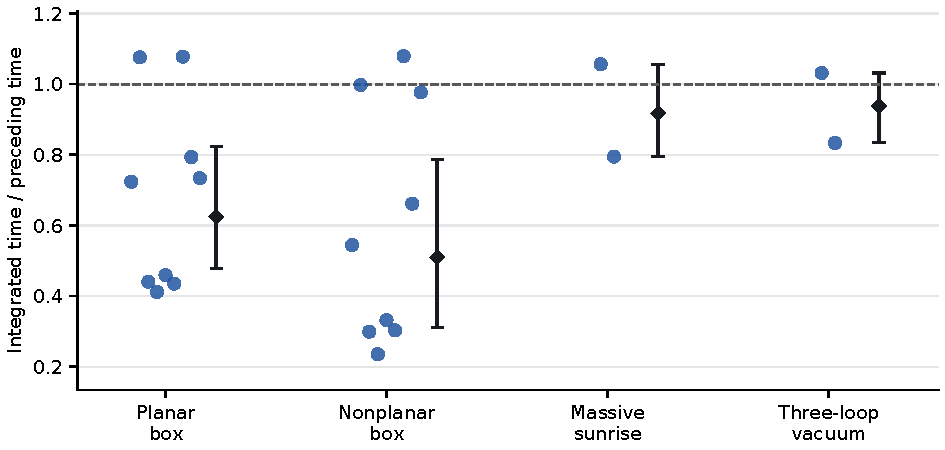
\includegraphics[width=.97\linewidth]{paper_figures/reconstruction_native.pdf}
\caption{Native speed changes depend on the physical request. Each circle shows the integrated-to-preceding ratio for one completed request. Diamonds show ratios of summed median times within each structure, with paired request-resampling intervals. Values below one mean less elapsed time.}
\label{notes-reconstruction-fig:reconstruction-native}
\end{figure}
\begin{figure}[!htbp]\centering
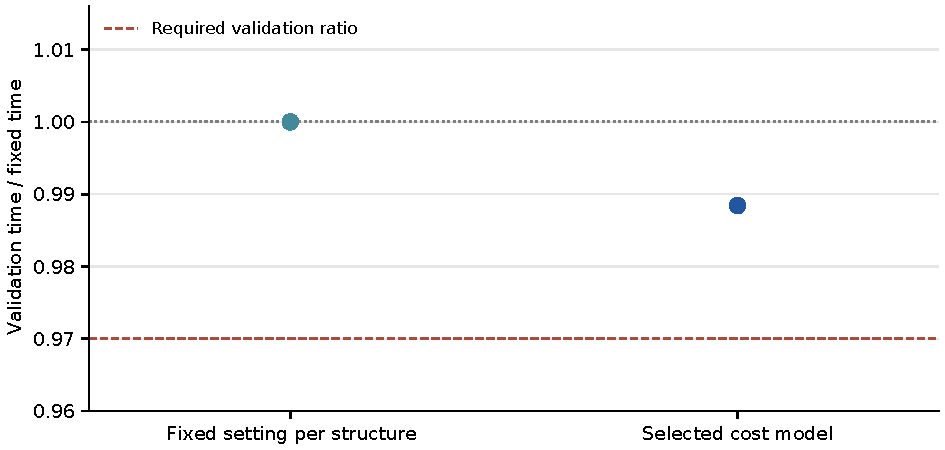
\includegraphics[width=.97\linewidth]{paper_figures/reconstruction_ml.pdf}
\caption{Separate validation determines whether the new model is used. The dashed threshold requires at least three percent less cost than the fixed setting selected for each structure. The current deployment retains the fixed settings because the model does not meet this condition.}
\label{notes-reconstruction-fig:reconstruction-ml}
\end{figure}

\subsection{Cumulative change and exact reductions}
The matched comparison across the last two extensions changes from 81.827 to 49.852 seconds on 75 completed requests. Its ratio is 0.609, with interval $[0.470,0.787]$, or 39.1\% less time at the point estimate. This result uses one input set and one timing procedure. It is a cumulative comparison with the earlier application, not with unmodified Kira, and it does not multiply percentages from older experiments.

The direct vacuum formulas and connected-tree recurrences remain active through thirteen loops. They provide rational master decompositions and explicit Gamma-function values in the domains derived in the appendices. The present analytic grid verifies their preservation while the new algebra method changes the native calculations. General coupled multiscale scattering through thirteen loops is outside this grid.
\begin{figure}[!htbp]\centering
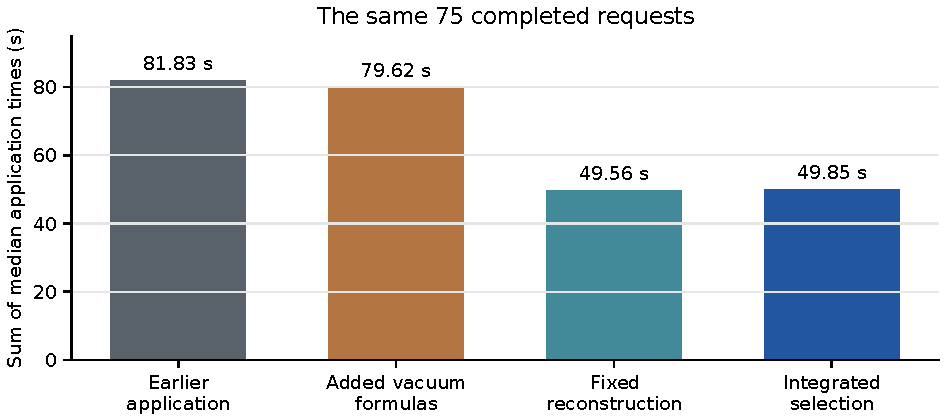
\includegraphics[width=.97\linewidth]{paper_figures/reconstruction_components.pdf}
\caption{Cumulative elapsed time is measured on the same requests for all four applications. The second application adds direct vacuum formulas; the third adds validated fixed reconstruction settings; the fourth applies the admitted selection procedure. The bars do not combine unrelated historical speed factors.}
\label{notes-reconstruction-fig:reconstruction-components}
\end{figure}
\begin{figure}[!htbp]\centering
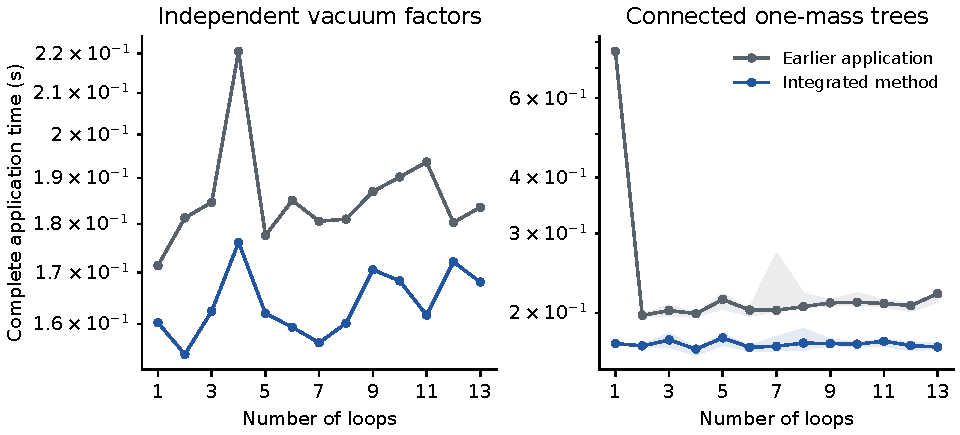
\includegraphics[width=\linewidth]{paper_figures/reconstruction_exact.pdf}
\caption{The analytic stage covers each loop order from one through thirteen in its stated domains. The left panel shows independent vacuum factors. The right panel shows connected one-mass trees, with the median over available shapes and their full range. Logarithmic time axes show the small complete application times without hiding their variation.}
\label{notes-reconstruction-fig:reconstruction-exact}
\end{figure}
\subsection{Completion and scope}
The timed outputs receive 18,132 exact coefficient comparisons. The integrated application has 0 unverified timed applications and 0 recorded unsuccessful inner native attempts. It uses reconstruction recovery 0 times. Reference preparation fails for 0 final requests. Application failure counts include a terminated run even when it cannot return an inner-attempt record.

The current native test measures new kinematic points and complete target batches within four known structures at two and three loops. Higher-loop evidence comes from the derived product and tree identities. It does not establish performance for every high-loop graph, every symbolic kinematic system, or unrestricted numerator powers. The measured configuration also depends on the tested processor and resource bounds. A finite model and setting search does not prove globally minimum time.
\subsection{Retained ML in the reconstruction workflow}
The additional paired comparison holds the new algebra settings fixed and switches the inherited learned choices to their existing fixed procedure. On 22 matched native requests, the fixed procedure takes 42.175 seconds and the learned procedure takes 41.448 seconds. Their ratio is 0.983, with interval $[0.951,1.003]$. This interval includes equal time, so the sample does not resolve a consistent additional learned saving. The recorded seed-attempt sequences differ on 14 requests. The learned and fixed procedures have 0 and 0 unverified applications, respectively. Across all three repetitions, their total times are 128.032 and 127.546 seconds. The distinction between total repeated time and summed medians illustrates the timing variation. This ablation has its own paired timings; its ratio is not multiplied into the cumulative result.

\begin{table}[!htbp]\centering\small
\caption{Inherited learned choices versus their existing fixed procedure, with the new reconstruction settings shared. The columns use matched completed requests within each structure.}
\label{notes-reconstruction-tab:reconstruction-retained}
\begin{tabularx}{\linewidth}{@{}Yrrrr@{}}\toprule
Structure & Paired & Fixed (s) & Learned (s) & Ratio\\\midrule
Planar box & 9 & 11.656 & 11.482 & 0.985 \\
Nonplanar box & 9 & 24.355 & 23.842 & 0.979 \\
Massive sunrise & 2 & 2.565 & 2.542 & 0.991 \\
Three-loop vacuum & 2 & 3.600 & 3.582 & 0.995 \\
All native requests & 22 & 42.175 & 41.448 & 0.983 \\
\bottomrule\end{tabularx}\end{table}


\subsection{The other learned interventions}
Table~\ref{notes-reconstruction-tab:retained-results} retains the main earlier controls needed to interpret the method. They use different workloads and cannot be multiplied into a cumulative speed factor. The equation-filter result supports that intervention on its tested domain, while the row results motivate its omission. The current combined experiment keeps equation filtering off and does not claim a joint seed-plus-equation gain.
\begin{table}[!htbp]\centering\small
\caption{Earlier measurements from this study, retained as separate evidence. A ratio below one means less time. Their full input definitions and measurements remain in the notes.}
\label{notes-reconstruction-tab:retained-results}
\begin{tabularx}{\linewidth}{@{}YYr@{}}\toprule
Intervention & Control and workload & Time ratio\\\midrule
Earlier native seed model & Fixed region, 32 box batches: 156.383 to 150.663 s & 0.963\\
Equation selection & Native filter, 24 new-index batches: 72.295 to 67.478 s & 0.933\\
Original learned row model & Native row choices, 84 trials & 1.305\\
Compiled row-cost policy & Native row choices; geometric mean & 0.982\\\bottomrule
\end{tabularx}
\end{table}
The earlier seed comparison has interval $[0.937,0.984]$, and the equation comparison has interval $[0.928,0.940]$. The compiled row policy has interval $[0.959,1.003]$, which includes equal time. These intervals use the resampling procedure recorded for each original study. The native row algorithm remains in the retained workflow.

\FloatBarrier


\section{Measured-cost learning}
\label{notes-reconstruction-app:shared}
For training request $i$ and action $a$, let $t_{ia}$ be measured elapsed time, $f_{ia}$ the fraction of unsuccessful repetitions, and $b_i$ the measured preceding-application time. We define the training cost and relative cost by
\begin{equation}
 C_{ia}=t_{ia}+f_{ia}b_i,\qquad y_{ia}=C_{ia}/b_i.
 \label{notes-reconstruction-eq:reconstruction-cost}
\end{equation}
The first expression adds the measured failed attempt and the estimated cost of recovery. The second expresses this cost relative to the same request's control. These are training definitions. The reserved comparison measures actual complete applications, including actual recovery.

The ensemble predicts the vector $\boldsymbol z_i=(y_{i1},\ldots,y_{i6},f_{i1},\ldots,f_{i6})$. It minimizes weighted squared error at its regression leaves, following the extremely randomized tree construction of Ref.~\cite{Geurts2006ExtraTrees}. For one component $z$ and a leaf containing requests $S$, its loss is $\sum_{i\in S}b_i(z_i-\mu)^2$. Differentiation with respect to $\mu$ gives
\begin{equation}
 0=2\sum_{i\in S}b_i(\mu-z_i),\qquad
 \widehat z(S)=\frac{\sum_{i\in S}b_i z_i}{\sum_{i\in S}b_i}.
 \label{notes-reconstruction-eq:reconstruction-leaf}
\end{equation}
For a cost component, inserting $z_i=C_{ia}/b_i$ gives
\begin{equation}
 \widehat y_a(S)=\frac{\sum_{i\in S}C_{ia}}{\sum_{i\in S}b_i},
 \qquad
 \arg\min_a\widehat y_a(S)=\arg\min_a\sum_{i\in S}C_{ia}.
 \label{notes-reconstruction-eq:reconstruction-leaf-choice}
\end{equation}
The denominator is independent of the action, which proves the second equality. Thus a leaf ranks actions by their aggregate measured cost on its requests. The ensemble averages the 32 leaf predictions. Weighting by $b_i$ gives slower baseline requests more influence, while relative costs permit one model to represent different physical structures. This local cost interpretation does not prove global minimum time on unseen requests.

Validation compares maximum depths 2, 4, and 6, minimum leaf populations 2 and 4, and predicted saving margins $\eta=0,0.05,0.10,0.20$. For the fixed action $b$ selected for a propagator structure, we choose the least predicted relative cost among actions with predicted failure fraction at most 0.02. We use that action $a_*$ only if
\begin{equation}
 \widehat y_{a_*}<(1-\eta)\widehat y_b.
 \label{notes-reconstruction-eq:reconstruction-margin}
\end{equation}
This inequality is the defined fractional saving condition. If no alternative satisfies it, the action remains $b$. A feature outside the training minimum or maximum uses the preceding procedure. Validation must then show a complete-cost ratio below 0.97 with no failed selected attempt before deployment enables the model. Failure scores describe observed training outcomes; a zero score does not certify an unseen reduction.

To specify the features, define target excess power $D=\sum_j\max(a_j-1,0)$, numerator rank $R=\sum_j\max(-a_j,0)$, and line count $P_T=\sum_j{\bf1}_{a_j>0}$. A line is incident on a loop momentum when that momentum occurs in its inverse propagator. The 29 features are listed in Table~\ref{notes-reconstruction-tab:reconstruction-features}. Every feature follows from the supplied indices and propagator definitions.
\begin{table}[!htbp]\centering\small
\caption{Inputs to the algebra-cost model. Means and extrema over targets use the complete requested batch.}
\label{notes-reconstruction-tab:reconstruction-features}
\begin{tabularx}{\linewidth}{@{}lY@{}}\toprule
Positions & Quantities\\\midrule
1--6 & Number of loops, external momenta, integral coordinates, physical propagators, symbolic external invariants, and $\log(1+n_T)$ for $n_T$ targets\\
7--13 & Maximum and mean $D$, maximum and mean $R$, minimum and maximum $P_T$, and number of distinct sectors\\
14--18 & Number of massive coordinates; number of physical lines containing several loops; maximum loop incidence per physical line; maximum physical-line incidence per loop; mean external-momentum incidence per coordinate\\
19--22 & Minimum $D$, minimum $R$, mean $P_T$, and maximum absolute index\\
23--25 & Mean excess power on massive coordinates; mean numerator rank weighted by loop incidence; mean excess power weighted by loop incidence\\
26--29 & Maximum sum of positive powers; maximum number of absent physical lines; maximum numerator and denominator bit lengths among rational masses and scalar products\\\bottomrule
\end{tabularx}\end{table}
The ordering within positions 7--10 is maximum $D$, maximum $R$, mean $D$, mean $R$. The remaining entries follow the listed order. The bit lengths describe the supplied rational numbers and do not encode a family identifier.

\section{Native reconstruction inputs}
\label{notes-reconstruction-app:reconstruction-inputs}
The planar and nonplanar boxes use Eqs.~\eqref{notes-direct-eq:planar-input} and \eqref{notes-direct-eq:nonplanar-input}, respectively. The high-rank targets are $(1,1,1,1,1,1,1,-u,-v)$ with $u,v\geq0$ and $1\leq u+v\leq4$. Each graph contributes fourteen training, six validation, and six reserved high-rank batches. The complete target sets differ between splits and exclude the preceding comparison batches. Individual target vectors can occur in more than one batch.

For batch index $i=0,\ldots,25$, define $j=i\bmod6$ and $q=\lfloor i/6\rfloor$. Let
\begin{align}
 (A_0,\ldots,A_5)&=(3,13,103,1009,10007,100003),\nonumber\\
 (B_0,\ldots,B_5)&=(7,19,107,1013,10009,100019).
 \label{notes-reconstruction-eq:reconstruction-scales}
\end{align}
We set $s=-(A_j+2q)$ and $t=-(B_j+4q)$ in both graphs, using each graph's scalar-product convention. Indices $0$--$13$ train the model, $14$--$19$ select it, and $20$--$25$ test it. These equations define the chosen input points. In the planar graph the fourth momentum is $-p_1-p_2-p_3$, and in the nonplanar graph it is $p_1+p_2-p_3$. Expanding their squares with the listed scalar products gives zero in both cases. The test batches are specified in Table~\ref{notes-reconstruction-tab:reconstruction-batches}.
\begin{table}[!htbp]\centering\small
\caption{Reserved high-rank target batches. The same $(u,v)$ sets and invariants enter both box routings. Every row defines a complete request for each graph.}
\label{notes-reconstruction-tab:reconstruction-batches}
\begin{tabularx}{\linewidth}{@{}rrrY@{}}\toprule
$i$ & $s$ & $t$ & Numerator powers $(u,v)$\\\midrule
20 & -109 & -119 & $(2,0), (0,2), (0,1)$ \\
21 & -1015 & -1025 & $(2,2), (0,4)$ \\
22 & -10013 & -10021 & $(3,1), (3,0), (2,1), (1,3), (0,1)$ \\
23 & -100009 & -100031 & $(3,1), (2,2), (2,1), (2,0), (1,2), (0,4)$ \\
24 & -11 & -23 & $(2,2), (2,1), (1,2), (1,1), (0,2), (0,1)$ \\
25 & -21 & -35 & $(2,1), (1,3), (1,2), (1,0), (0,2), (0,1)$ \\
\bottomrule\end{tabularx}\end{table}

For the lower-rank box requests, the sector corner is $(1,1,1,1,1,1,1,0,0)$. A numerator request uses the supplied first-rank auxiliary targets, and a raised-power request increases one physical index. Table~\ref{notes-reconstruction-tab:reconstruction-low-targets} lists their precise target vectors. Their profiles are $h=27701,27713$ for training, $27733$ for validation, and $27739$ for testing, with the low-rank kinematics of Appendix~\ref{notes-direct-app:families-new}.

The sunrise family has loop momenta $(\ell_1,\ell_2)$ and one external momentum $p$. Its inverse-propagator momenta and squared masses are
\begin{equation}
 (Q_1,\ldots,Q_5)=(\ell_1,\ell_2,p-\ell_1-\ell_2,p-\ell_1,p-\ell_2),
 \qquad (m_1^2,\ldots,m_5^2)=(3,7,13,0,0).
 \label{notes-reconstruction-eq:reconstruction-sunrise}
\end{equation}
The first three coordinates are physical denominators and the last two are auxiliary. The three-loop vacuum uses
\begin{align}
 (Q_1,\ldots,Q_6)&=(\ell_1,\ell_2,\ell_3,\ell_1-\ell_2,\ell_2-\ell_3,\ell_1-\ell_3),\nonumber\\
 (m_1^2,\ldots,m_6^2)&=(1,1,1,13,13,2h+53).
 \label{notes-reconstruction-eq:reconstruction-vacuum}
\end{align}
All six coordinates are physical. Both structures use the same profile split as the low-rank boxes. For the sunrise, $p^2=-1009-12h$. These assignments specify test families, rather than universal relations between masses and invariants. In every native request the kinematic quantities are fixed rational numbers and $d$ remains symbolic, so the coefficients belong to $\Q(d)$. This test does not reconstruct general symbolic scattering invariants.

\begin{table}[!htbp]\centering\small
\caption{Lower-rank reserved targets. Training and validation use the same index patterns at different physical points. A corner request contains the all-unit physical sector.}
\label{notes-reconstruction-tab:reconstruction-low-targets}
\begin{tabularx}{\linewidth}{@{}lY@{}}\toprule
Structure and request & Target indices\\\midrule
Planar box, corner & $(1,1,1,1,1,1,1,0,0)$ \\
Planar box, numerator & $(1,1,1,1,1,1,1,0,-1), (1,1,1,1,1,1,1,-1,0)$ \\
Planar box, raised power & $(1,1,1,1,1,2,1,0,0), (1,1,1,1,1,1,2,0,0), (2,1,1,1,1,1,1,0,0)$ \\
Nonplanar box, corner & $(1,1,1,1,1,1,1,0,0)$ \\
Nonplanar box, numerator & $(1,1,1,1,1,1,1,0,-1), (1,1,1,1,1,1,1,-1,0)$ \\
Nonplanar box, raised power & $(1,1,1,1,1,2,1,0,0), (1,1,1,1,1,1,2,0,0), (2,1,1,1,1,1,1,0,0)$ \\
Sunrise, corner & $(1,1,1,0,0)$ \\
Sunrise, raised power & $(1,2,1,0,0), (1,1,2,0,0), (2,1,1,0,0)$ \\
Vacuum, corner & $(1,1,1,1,1,1)$ \\
Vacuum, raised power & $(1,2,1,1,1,1), (1,1,2,1,1,1), (1,1,1,2,1,1)$ \\
\bottomrule\end{tabularx}\end{table}

The protected native bases consist of the integral indices below. Each listed vector $\boldsymbol b$ denotes $M_{\boldsymbol b}=I_{\boldsymbol b}$ in its corresponding family. The independently prepared symbolic and reconstructed calculations use the same basis for each request. The lists specify the comparison basis; they do not assert a proof of global master independence from a finite seed system.

Planar box:\[\begin{aligned}\{&(0,0,1,1,0,0,1,0,0),(0,1,0,0,0,1,1,0,0),\\&(0,1,0,1,1,0,1,0,0),(0,1,1,1,0,1,1,0,0),\\&(1,0,1,1,1,0,0,0,0),(1,1,1,0,0,1,1,0,0),\\&(1,1,1,1,1,1,1,-1,0),(1,1,1,1,1,1,1,0,0)\}.\end{aligned}\]

Nonplanar box:\[\begin{aligned}\{&(0,0,1,1,1,1,0,0,0),(0,1,0,0,1,1,0,0,0),\\&(0,1,1,1,1,1,1,0,0),(1,0,0,1,0,1,0,0,0),\\&(1,0,1,1,1,1,0,0,0),(1,1,0,0,0,0,1,0,0),\\&(1,1,0,1,0,1,1,0,0),(1,1,0,1,1,1,0,0,0),\\&(1,1,1,0,1,0,1,0,0),(1,1,1,1,0,0,1,0,0),\\&(1,1,1,1,1,1,1,-1,0),(1,1,1,1,1,1,1,0,0)\}.\end{aligned}\]

Sunrise, basis 1:\[\begin{aligned}\{&(0,1,1,0,0),(1,0,1,0,0),\\&(1,1,0,0,0),(1,1,1,-1,0),\\&(1,1,1,0,-1),(1,1,1,0,0),\\&(1,1,2,0,0)\}.\end{aligned}\]

Sunrise, basis 2:\[\begin{aligned}\{&(1,1,1,0,0)\}.\end{aligned}\]

Three-loop vacuum, basis 1:\[\begin{aligned}\{&(0,1,1,1,0,1),(0,1,1,1,0,2),\\&(0,1,1,2,0,1),(1,0,0,1,1,1),\\&(1,0,1,1,0,1),(1,0,1,1,1,0),\\&(1,0,1,1,1,1),(1,0,1,1,2,0),\\&(1,1,0,1,0,1),(1,1,0,1,1,0),\\&(1,1,0,1,1,1),(1,1,1,0,0,1),\\&(1,1,1,1,0,0),(1,1,1,1,0,1),\\&(1,1,1,1,1,0),(1,1,1,1,1,1)\}.\end{aligned}\]

Three-loop vacuum, basis 2:\[\begin{aligned}\{&(1,1,1,1,1,1)\}.\end{aligned}\]


\section{Coefficient reconstruction}
\label{notes-reconstruction-app:reconstruction-algebra}
Kira and FireFly provide the finite-field algorithms used here~\cite{Kira2,FireFly2019,FireFly2020}. To explain the relation to an exact rational coefficient, suppose
\begin{equation}
 r(d)=P(d)/Q(d),\qquad
 P(d)=\sum_{j=0}^{n}p_jd^j,\quad Q(d)=\sum_{j=0}^{m}q_jd^j.
 \label{notes-reconstruction-eq:reconstruction-rational}
\end{equation}
One nonzero denominator coefficient fixes the overall normalization. At a nonsingular point $d=z$ modulo a prime, a numerical reduction returns $r(z)$. Multiplying by the denominator gives the linear constraint
\begin{equation}
 \sum_{j=0}^{n}p_jz^j-r(z)\sum_{j=0}^{m}q_jz^j=0\pmod p.
 \label{notes-reconstruction-eq:reconstruction-sample}
\end{equation}
This follows directly from Eq.~\eqref{notes-reconstruction-eq:reconstruction-rational}. With correct degree bounds and sufficiently many independent nonsingular samples, the constraints determine the normalized coefficients over the field. Combining suitable primes and reconstructing rational numbers then supplies rational coefficients~\cite{FireFly2019,FireFly2020}. FireFly determines the necessary information adaptively; our model chooses the native procedure and probe batch size.

The field operations are exact, while reconstruction termination relies on its degree discovery and checks. Our evaluation therefore also subtracts every reconstructed coefficient from a separately computed symbolic reference and requires the rational difference to vanish. This checks the actual tested answer. Neither a model score nor a successful reduction to the supplied basis alone proves every coefficient for an arbitrary unseen request.


\section{Development checks and excluded trials}
The development study compared direct symbolic algebra, full finite-field reconstruction, and reconstruction restricted to back-substitution. Full reconstruction was faster than reconstructed back-substitution on all four initial box requests, so the six training actions retain symbolic algebra and five full-reconstruction probe batch sizes. Additional development requests covered sector corners, numerators, raised powers, massive sunrise integrals, and a three-loop vacuum. Some separate probe-size pilots used different nodes; their individual timings were used to retain candidates, rather than to claim a precise cross-node speed ratio.

Two initial coefficient comparisons used different master bases. A separate symbolic reduction in the protected application basis resolved both comparisons, and all affected coefficients agreed. The original output and the corrected comparison remain preserved.

The first expanded reference regions generated substantially more equations and reached the reference time limit. Further complete-region reference checks also reached their bound on high-rank nonplanar requests. The preceding application completed these requests symbolically and supplied the independent coefficients used to check reconstruction. These failures belong to reference preparation, outside the complete application timer.

An early nonplanar input generator used the planar sign convention for the third external momentum. Its fourth leg therefore did not satisfy the intended massless condition. Those inputs and unsuccessful preparation trials were excluded before estimator fitting. The corrected generator checks all 76 box inputs across the three splits: the three listed legs and the convention-dependent fourth leg are massless, and invariant metadata agree with the scalar products. The reserved outcomes did not select the correction or the trained model.
% RECONSTRUCTION UPDATE END
% END CURRENT WORKFLOW UPDATE
% BEGIN CURRENT WORKFLOW UPDATE
% BATCH APPLICATION UPDATE BEGIN
\section{Processing a collection together}
\label{notes-shared-application:method}
The preceding comparison loads the application separately for each request. A further test processes the same 75 requests in one call, so numerical routines, mathematical objects, and learned policies can remain in memory. The shared call also uses one bounded output stream for the collection. Every request still receives its own reduction, and the exact formulas, model weights, algebra settings, and protected bases remain unchanged. The input supplies no reference coefficients.

We compare separate and shared calls for both the earlier and current methods. The earlier method precedes the direct vacuum formulas and reconstruction extension. Each comparison uses three complete repetitions. Two workers run on the same Intel Gold compute node, with one computation thread per application. We alternate method order and reverse the request order in the middle repetition. Time includes loading, all reductions, output, exit, reading the returned data, and cleanup; the separate-call total sums those complete call times. Independent reference comparisons remain outside both timers. These implementation checks reuse the previously verified physical inputs.

\begin{table}[htbp]
\centering\small
\caption{Complete time for the same collection of 75 requests. Each value is the median of three full-collection times. The range contains all three repetitions and is not a confidence interval. Every method completes every request in every repetition.}
\label{notes-shared-application:times}
\begin{tabular}{lrr}
\toprule
Method & Median (s) & Observed range (s)\\
\midrule
Earlier method, separate calls & 96.355 & 94.794--103.077 \\
Current method, separate calls & 58.980 & 57.669--59.163 \\
Earlier method, shared call & 70.051 & 69.210--71.538 \\
Current method, shared call & 37.247 & 36.713--38.256 \\
\bottomrule
\end{tabular}
\end{table}

For the current method, shared processing changes complete time from 58.980 to 37.247 seconds, a ratio of 0.632. The matched cumulative comparison changes from 96.355 seconds for the earlier separate calls to 37.247 seconds for the current shared call. When both methods share their setup, the earlier method takes 70.051 seconds and the current method takes 37.247 seconds. This control preserves a comparison of the algebraic changes after both methods receive the same setup benefit. These collection-level medians differ from the sum of per-request medians in Table~\ref{notes-reconstruction-tab:reconstruction-times} and come from a separate timing job. We compare each method with the controls measured in the same experiment.

All 900 request executions pass 18,132 coefficient comparisons, with zero failed applications. Shared processing preserves every recorded reconstruction choice. This change comes from reuse within a call. The models and verified physical domain remain those of the preceding comparison.


\subsection{Preparation checks}
Two earlier batch-test submissions stopped because the reference checker loaded its dependencies in an order that assumed a native request came first. The first stopped before timing; the second reached the reversed-order reference check and retained a completed forward control. We preserved the interrupted records and repeated the complete comparison after explicitly initializing the checker and checking its analytic path before timing. The reduction application, mathematical methods, model weights, and physical requests remained unchanged. The final timing table uses the complete comparison after this correction.

A subsequent timing audit found that the separate-call timer included reading the returned output and cleanup, while the initial shared-call timer stopped at process exit. We preserved that preliminary comparison, aligned both timing boundaries, and repeated all four methods. The final table uses the aligned timers. The application and mathematical outputs were unchanged.

% BATCH APPLICATION UPDATE END
% END CURRENT WORKFLOW UPDATE
% BEGIN CURRENT WORKFLOW UPDATE
\section{Exact reduction of a one-scale massless triangle}
\label{notes-triangle:app:triangle}
The on-shell triangle has a Gamma-function representation~\cite{DavydychevOsland1998}. We derive its coefficient in our normalization to specify the signs and the master basis used by the implementation. Let
\begin{equation}
 T_{abc}(Q,d)=\int\frac{d^d k}{i\pi^{d/2}}
 \frac{1}{[k^2+i0]^a[(k-p_1)^2+i0]^b[(k-p_1-p_2)^2+i0]^c},
 \label{notes-triangle:eq:triangle-definition}
\end{equation}
where $p_1^2=p_2^2=0$, $Q=-(p_1+p_2)^2>0$, and $a,b,c$ are propagator powers. Write $A=a+b+c$ and $h=d/2$. For initially positive powers in a convergence region, Feynman parametrization and the shifted loop integral give
\begin{align}
 T_{abc}&=\frac{(-1)^A\Gamma(A-h)}{\Gamma(a)\Gamma(b)\Gamma(c)}
 \int_{x_j\geq0} d^3x\,\delta(1-x_1-x_2-x_3)
 x_1^{a-1}x_2^{b-1}x_3^{c-1}(Qx_1x_3)^{h-A}.
 \label{notes-triangle:eq:triangle-parameters}
\end{align}
The only nonzero squared momentum difference is between the first and third propagators, which gives the factor $Qx_1x_3$. The Dirichlet integral follows by writing three Gamma integrals and changing their variables to a common scale and three fractions. Explicitly, the substitution $t_j=u x_j$ in $\prod_j\int_0^\infty dt_j\,t_j^{z_j-1}e^{-t_j}$ gives
\begin{equation}
 \int d^3x\,\delta(1-\textstyle\sum_j x_j)\prod_jx_j^{z_j-1}
 =\frac{\prod_j\Gamma(z_j)}{\Gamma(\sum_jz_j)}.
 \label{notes-triangle:eq:triangle-dirichlet}
\end{equation}
Applying this identity with $z_1=h-b-c$, $z_2=b$, and $z_3=h-a-b$ yields
\begin{equation}
 T_{abc}=(-1)^A Q^{h-A}
 \frac{\Gamma(A-h)\Gamma(h-b-c)\Gamma(h-a-b)}
 {\Gamma(a)\Gamma(c)\Gamma(d-A)}.
 \label{notes-triangle:eq:triangle-gamma}
\end{equation}
Dimensional continuation defines the expression outside the initial convergence region. The limit $b\to0$ gives the two-point integral obtained by removing the middle propagator. Its unit-power value is
\begin{equation}
 B(Q,d)=T_{101}=Q^{h-2}
 \frac{\Gamma(2-h)\Gamma(h-1)^2}{\Gamma(d-2)}.
 \label{notes-triangle:eq:triangle-bubble}
\end{equation}
For positive integers $a,c$ and a nonnegative integer $b$, division of Eq.~\eqref{notes-triangle:eq:triangle-gamma} by Eq.~\eqref{notes-triangle:eq:triangle-bubble} gives a rational coefficient. To evaluate it with finite products, define
\begin{equation}
 (z)_n=\frac{\Gamma(z+n)}{\Gamma(z)}=
 \begin{cases}
 \prod_{j=0}^{n-1}(z+j),&n\geq0,\\
 \displaystyle\frac{1}{\prod_{j=1}^{-n}(z-j)},&n<0.
 \end{cases}
 \label{notes-triangle:eq:triangle-pochhammer}
\end{equation}
The empty product equals one. The identity follows by repeated application of $\Gamma(z+1)=z\Gamma(z)$ and gives
\begin{align}
 T_{abc}&=R_{abc}(Q,d)B(Q,d),\\
 R_{abc}&=\frac{(-1)^A Q^{2-A}}{(a-1)!(c-1)!}
 (2-h)_{A-2}(h-1)_{1-a-b}(h-1)_{1-b-c}(d-A)_{A-2}.
 \label{notes-triangle:eq:triangle-rational}
\end{align}
For example, $R_{111}=2(d-3)/[Q(d-4)]$. Increasing $a$ by one gives the recurrence
\begin{equation}
 R_{a+1,b,c}=-\frac{(A-h)(d-A-1)}{Qa(h-a-b-1)}R_{abc},
 \label{notes-triangle:eq:triangle-recurrence}
\end{equation}
which supplies a separate exact check on the finite-product calculation. If $a=0$ or $c=0$, the remaining massless denominators have no nonzero external invariant. Those sectors vanish in dimensional regularization~\cite{Weinzierl2022}.

The implementation checks all masses and pairwise momentum differences before using this formula. It accepts rational $Q>0$, powers from zero through four, and $A\leq8$. It rejects cut propagators, additional occupied lines, and negative indices. For independent loop components with no occupied cross-loop denominator, the product measure then gives
\begin{equation}
 \prod_{j=1}^{L}T_{a_jb_jc_j}(Q_j,d)
 =\left[\prod_{j=1}^{L}R_{a_jb_jc_j}(Q_j,d)\right]
 \prod_{j=1}^{L}B(Q_j,d).
 \label{notes-triangle:eq:triangle-product}
\end{equation}
The proof follows by factoring the integrand and measure in a common convergence region and then continuing the result analytically. If the requested integer powers have no common convergence region in $d$, we first allow the propagator powers to vary independently. Equation~\eqref{notes-triangle:eq:triangle-gamma} gives their meromorphic continuation, which defines the product at the requested powers and dimension. This extension covers products through thirteen loops in the implementation. The implementation retains this product of component coefficients instead of expanding it into a larger polynomial. It supplies no formula for a general connected thirteen-loop scattering graph.
\subsection{Inputs for the additional comparison}
The four native propagator structures are those in Appendix~\ref{notes-reconstruction-app:reconstruction-inputs}. For the new planar and nonplanar box requests, the invariants are $s=-(137+6i)$ and $t=-(167+4i)$, with the incoming/outgoing momentum conventions stated there. Training uses $i=2,\ldots,13$, validation uses $i=14,\ldots,18$, and reserved tests use $i=19,\ldots,23$. Each box target has powers $(1,1,1,1,1,1,1,-a,-b)$. The reserved pairs are listed below; both box structures use the same pairs at each $i$.
\begin{center}\small\begin{tabular}{cl}\toprule
$i$ & Pairs $(a,b)$ in the target request\\\midrule
19 & $(3,0), (2,2), (0,2)$ \\
20 & $(4,0), (3,1)$ \\
21 & $(4,0), (1,2), (0,2), (0,1)$ \\
22 & $(3,1), (2,1), (0,2)$ \\
23 & $(2,1), (2,0), (1,0), (0,4), (0,2), (0,1)$ \\
\bottomrule\end{tabular}\end{center}
The sunrise masses remain $(3,7,13)$ and its external invariant is $p^2=-386221-12i$. The three-loop vacuum masses remain $(1,1,1,13,13,64255+2i)$. These families use the same index splits. Even $i$ requests the sector corner, and odd $i$ requests the raised-power targets defined for that structure. Full physical inputs differ between splits. Graph structures and individual index vectors recur; box target batches are distinct across the new splits.

For a triangle product with $L$ loops, every factor has $Q=101+2L$. We choose factor powers from $(1,1,1)$, $(2,1,1)$, $(1,2,1)$, $(1,1,2)$, $(2,2,1)$, $(1,0,1)$, and $(2,0,2)$. We form six products per loop order and remove duplicate full targets. Cross-loop auxiliary powers are zero. Seven additional single-loop requests use $Q=211+2j$, $j=1,\ldots,7$, and the targets $(1,1,1)$, $(1+(j\bmod3),1+(j\bmod2),1)$, $(1,0,1)$, $(2,0,1)$, and $(0,1,1)$, again with duplicate targets removed.

The preceding triangle basis uses unit-power triangle masters. For verification, each such master is replaced by $2(d-3)B/[Q(d-4)]$, and independent components multiply. Kira provides a separate bubble-basis reference for each new single-loop request. The higher-loop comparison combines this exact basis conversion with the product derivation and independent Gamma-function checks.
\subsection{A direct one-scale triangle formula}
A massless triangle with two lightlike external momenta admits an explicit Gamma-function value~\cite{DavydychevOsland1998}. We use this identity to return both its reduction coefficient and its analytic value. Let $T_{abc}$ have denominators $k^2$, $(k-p_1)^2$, and $(k-p_1-p_2)^2$, with $p_1^2=p_2^2=0$ and $Q=-(p_1+p_2)^2>0$. The integers $a,b,c$ are their powers. With $B(Q,d)=T_{101}$, the unit-power example is
\begin{equation}
 T_{111}=\frac{2(d-3)}{Q(d-4)}B(Q,d).
 \label{notes-triangle:eq:triangle-main}
\end{equation}
Appendix~\ref{notes-triangle:app:triangle} derives the general coefficient as a finite product of linear factors in $d$ and gives the Gamma-function value of $B$. The code accepts nonnegative powers through four with $a+b+c\leq8$, rational $Q>0$, and no extra occupied denominator. It also treats independent products of accepted triangles through thirteen loops.

The preceding application already returned analytic ratios to a triangle master on these inputs. The new implementation evaluates the coefficient directly in a bubble basis and supplies its explicit analytic value. We compare the two outputs after an exact basis conversion, and we also compare the single-loop results with Kira. The timing comparison therefore measures the change from the preceding analytic application, including its setup, rather than attributing all of the gain to avoided IBP elimination.
\subsection{A further native cost-model comparison}
The new native study tests whether the preferred probe batch size changes with the requested integrals. We measure 48 training requests and 20 validation requests across the same planar box, nonplanar box, sunrise, and three-loop vacuum structures. For the two-loop families, the five actions are the preceding application and full reconstruction with probe batch sizes 1, 4, 8, and 16. One three-loop training comparison failed and could not be reproduced by the subsequent symbolic and reconstruction checks. We therefore retain the preceding application for the vacuum structure and exclude its candidate reconstruction costs from model fitting. The fitted training set contains 36 two-loop requests; the complete comparison retains all four structures. Each action retains the preceding learned seed procedure, exact algebra, and bounded recovery. Complete action times include the initial choice and any recovery.

We fit 32 extremely randomized trees~\cite{Geurts2006ExtraTrees} to predict each action's complete time relative to the preceding application. Baseline seconds weight the squared regression error. Validation selects tree depth from 2, 4, and 6, minimum leaf population from 2 and 4, and the required predicted saving from zero, five, and ten percent. The fixed control selects its action separately for each propagator structure. We enable the learned selector only if it saves at least three percent on validation and selects no failed algebra procedure. This condition tests the value of the added model beyond structure-dependent settings. We use the same 29 physical features and weighted cost objective as Appendix~\ref{notes-reconstruction-app:shared}. Here the training cost is the measured complete time, including actual recovery. The model predicts five relative costs; the stated structure guard and observed validation outcomes determine admission.

Summed action costs on validation give 46.438 seconds for the fixed control and 46.495 seconds for the best fitted selector. The additional native cost selector does not pass the validation condition. The application therefore uses the validated fixed settings and retains the fitted model for inspection.

We also test the preceding nonplanar equation classifier with the new reconstruction setting at its frozen threshold of 0.05. Five validation requests with two repetitions give 9.824 seconds without this additional filter and 16.807 seconds with it, including recovery. The classifier skips 17,808 of 53,430 candidate equation constructions, but all ten filtered attempts fail the prescribed-master-basis check and require recovery. We therefore leave this additional filter disabled; the earlier seed policy remains active.
\subsection{Direct triangles and refined native choices}
\label{notes-triangle:sec:triangle-results}
We freeze the added formula and cost policy before testing 40 new requests. Twenty contain native two- or three-loop reductions, and twenty contain single triangles or independent triangle products. The product tests cover every loop order from one through thirteen. We measure three fresh-process repetitions for each request and method. These first measurements retain the original runtime monitor. The preceding application, the new fixed control, and the new integrated method receive the same physical inputs. Times include application loading, model use where enabled, algebra, output reading, and cleanup. Independent coefficient comparisons remain outside all timers.

\begin{table}[htbp]\centering\small
\caption{New reserved requests. Times sum per-request medians of three complete calls. The ratio divides new time by preceding time.}
\label{notes-triangle:tab:triangle-times}
\begin{tabular}{lrrrr}\toprule
Requests & Number & Preceding (s) & New (s) & Ratio\\\midrule
One-scale triangles and products & 20 & 5.231 & 4.269 & 0.816 \\
Planar boxes & 5 & 10.829 & 8.792 & 0.812 \\
Nonplanar boxes & 5 & 17.214 & 13.123 & 0.762 \\
Massive sunrise & 5 & 10.215 & 10.265 & 1.005 \\
Three-loop vacuum & 5 & 14.277 & 14.399 & 1.009 \\
\bottomrule\end{tabular}\end{table}

The native requests give a total-time ratio of 0.887, with a paired request-bootstrap interval of $[0.743,1.010]$. The integrated-to-fixed ratio is 1.010, with interval $[0.990,1.029]$. Both new methods use the same fixed choices because the added selector is disabled. Their timing difference does not measure a new ML gain.
 The seven-loop product request has a time ratio of 1.077 in this fresh-process comparison. The measurements therefore include a slower triangle case, and they do not establish a monotonic trend with loop order.

\begin{figure}[htbp]\centering
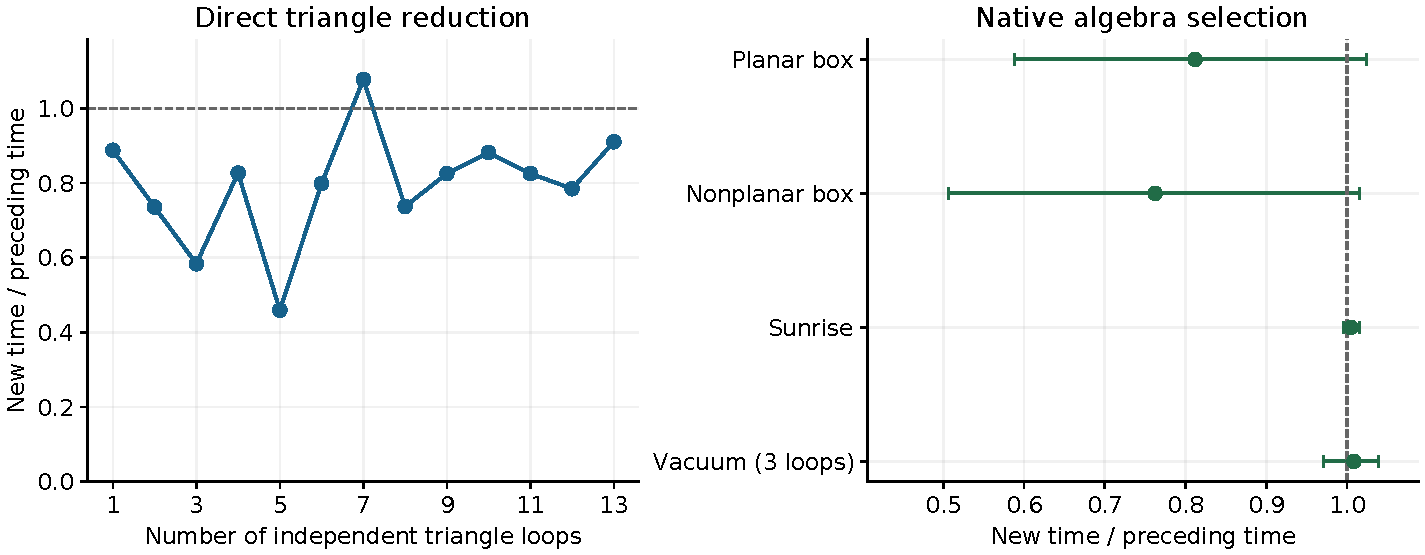
\includegraphics[width=\linewidth]{paper_figures/triangle_extension.pdf}
\caption{Complete-time ratios on the new requests. The dashed line marks equal time. The left panel shows the direct triangle implementation at each tested product loop order. The right panel shows native requests by propagator structure, with paired request-bootstrap intervals. Product tests do not establish connected higher-loop scattering performance.}
\label{notes-triangle:fig:triangle-extension}
\end{figure}

We also compare shared calls containing these 40 requests and the 53 preceding analytic regression requests. This preserves the setup benefit of the previously deployed method. Three complete repetitions use alternating method order and reverse the request order in the middle repetition. Two workers share an Intel Gold compute node, with one computation thread per application. The collection timer includes loading, all reductions, output reading, and cleanup.
\begin{table}[htbp]\centering\small
\caption{Shared-call time for the matched collection of 93 requests. The interval is the observed range of three complete repetitions, not a confidence interval.}
\label{notes-triangle:tab:triangle-batch}
\begin{tabular}{lrr}\toprule
Method & Median (s) & Observed range (s)\\\midrule
Preceding application & 46.642 & 46.337--48.713 \\
New fixed control & 40.561 & 39.524--46.243 \\
New integrated method & 40.696 & 40.194--41.472 \\
\bottomrule\end{tabular}\end{table}

The new-to-preceding collection ratio is 0.873. All 1,250 tested application results pass 19,946 exact coefficient comparisons after the stated basis conversion. The timed native procedures record 7 unsuccessful internal attempts across the fresh-call and shared-call comparisons; their recovery costs remain inside the timers. The separate formula checks add 120 high-precision Gamma-function comparisons, 4 exact index-shift checks, and 77 product checks. Native one-loop comparisons and the derivation support the triangle identity; the product tests check its separated-loop implementation.

\subsection{Final complete-call comparison}
A native reduction removes temporary files while it runs. The earlier resource monitor could stop a reduction if a directory disappeared during its inspection. We change the monitor to tolerate removal while preserving its storage bound. A controlled check reproduces the old exception and verifies the new behavior. This change affects runtime supervision and leaves the algebra and learned decisions unchanged.

We compare the preceding published application, the new mathematical method with the original monitor, and the final application with the corrected monitor on the same 93 requests. Each method runs three times on the same compute node with one worker, rotating method order, and reversed request order in the middle repetition. A preceding two-worker comparison showed timing differences larger than the measured monitor cost. It also stopped when recovery in the preceding application returned a 20-integral basis instead of the 16-integral reference basis for one vacuum request. We retain that failed comparison separately. The complete serial check uses every planned request and method. The complete timer includes unsuccessful internal attempts and recovery. Independent comparisons check the saved exact coefficients outside the timer.
\begin{table}[htbp]\centering\small
\caption{Final matched shared-call comparison. Times are complete collection times. The range shows the three observations. Internal failures count attempts across all three repetitions.}
\label{notes-triangle:tab:triangle-final}
\begin{tabular}{lrrrr}\toprule
Method & Median (s) & Mean (s) & Range (s) & Failures\\\midrule
Preceding application & 45.091 & 45.230 & 44.783--45.817 & 0 \\
New method, original monitor & 42.932 & 42.624 & 40.351--44.589 & 0 \\
Final application & 41.137 & 41.029 & 40.723--41.227 & 0 \\
\bottomrule\end{tabular}\end{table}
The final-to-preceding median ratio is 0.912, which reduces time by 8.8 percent on this collection. The final-to-original-monitor ratio is 0.958. All 837 application results pass 13,401 exact coefficient comparisons. This finite timing comparison does not prove a universal speedup or a globally shortest reduction.

The preceding parallel monitor comparison used two workers and stopped at the third published-application collection after the vacuum basis mismatch. Its recorded outputs pass 650 of 651 request comparisons. Its two complete matched repetitions give a final-to-published ratio of 0.847, and a corrected-to-original-monitor ratio of 1.131. The controlled serial repetition retains every physical input and algorithm. It changes the worker schedule to examine the unexplained timing difference. These two comparisons are reported separately.

\subsection{Verification imports}
Two verification helpers initially imported historical modules with the same names. We corrected these imports without changing the application, fitted model, or physical test inputs. We retained the completed timings and rechecked the saved results. The runtime-monitor comparison uses the corrected checks.

\subsection{Preparation checks and conservative admission}
The first native collection stopped at the three-loop vacuum request with squared masses $(1,1,1,13,13,64269)$. A probe batch size of eight disagreed with the preceding reference in the coefficient comparator. The collector stopped before it saved that candidate output, so its original difference cannot be reconstructed from the surviving record. The reference and failure log remain available. We corrected the collector to save a failed output before stopping.

Independent reruns compared symbolic algebra and several reconstruction settings. The original reference agreed with the symbolic result. Additional repetitions checked the disputed setting at four nearby mass profiles. These diagnostics did not justify treating the original failed check as a measured speedup. The new cost selector therefore retains the preceding application for this three-loop structure. The reserved comparison tests that conservative configuration. Independent symbolic reductions also check every action record used for fitting and validation.

% END CURRENT WORKFLOW UPDATE
\bibliographystyle{unsrt}
% BEGIN CURRENT WORKFLOW UPDATE
\let\OriginalNotesBibliography\bibliography
\renewcommand{\bibliography}[1]{\OriginalNotesBibliography{#1,notes_additional_references}}
% END CURRENT WORKFLOW UPDATE
\bibliography{references,type_specialist_references}

\end{document}
